\documentclass[
	a4paper, % Format du livre
	fontsize=11pt, % Taille de la police (texte de base)
	twoside=true, % Utiliser des mises en page différentes pour les pages paires et impaires (en particulier, si twoside=true, la colonne de marge sera toujours à l'extérieur).
	% open=any, % Si twoside=true, décomplétez ceci pour forcer les nouveaux chapitres à commencer sur n'importe quelle page, et pas seulement sur la page de droite (impaire).
	chapterentrydots=true, % Décommenter pour afficher les points du nom du chapitre au numéro de page dans la table des matières
	numbers=noenddot, % Commenter pour afficher des points après les numéros de chapitre ; les arguments les plus courantes pour cette option sont : enddot, noenddot et auto (voir la documentation KOMAScript pour une explication approfondie).
]{kaobook}

\usepackage[T1]{fontenc} % Encodage de la police pour les caractères internationaux

\usepackage{anyfontsize} % Pour le titre de la page de couverture



% Pour faire des pages blanches
\usepackage{afterpage}
\newcommand\pageblanche{
    \null
    \thispagestyle{empty}
    \addtocounter{page}{-1}
    \newpage
}

% Load the bibliography package
% \usepackage[natbib,refsection=chapter]{biblatex}
\usepackage{kaobiblio}
\addbibresource{main.bib} % Bibliography file

% Load mathematical packages for theorems and related environments
\usepackage[framed=true]{kaotheorems}

%%%% Ajoute par Alain pour pouvoir compiler le kaorefs %%%%
\usepackage[french]{babel}

\usepackage[dvipsnames]{xcolor}
\usepackage{ragged2e}

\usepackage{pdfpages}

% Pour la fonction Gamma
\usepackage{pgfplots}
\pgfplotsset{compat=newest}

% Pour la figure homothétie
\usepackage{tkz-euclide}

\usepackage{hyperref}
\hypersetup{
    colorlinks=true,
    linkcolor=blue,
    filecolor=magenta,      
    urlcolor=cyan
}
\usepackage{multicol}
\usepgfplotslibrary{fillbetween}

\usepackage{tikz}
\usetikzlibrary{automata, 
                decorations.pathreplacing, % pour les curly braces de la fig du déterminant
                calligraphy, % pour les curly braces de la fig du déterminant
                arrows, % customizing arrows
                positioning, % positioning nodes
                calc,
                bending, % figure racines troisième de l'unité
                matrix % critère de nilpotence par la trace
                }
% Pour le schéma de la preuve de la densité des matrices diagonalisables
\usetikzlibrary{decorations.markings,arrows}
\tikzset{
    arrowMe/.style={
        postaction=decorate,
        decoration={
            markings,
            mark=at position .45 with {\arrow[thick]{#1}}
        }
    }
}
                
% Pour la figure de projection orthogonale
%\usepackage[active,tightpage]{preview}

% Pour pouvoir enlever l'indentation dans un itemize
% https://tex.stackexchange.com/questions/131637/no-indentation-for-non-item-within-itemize
\newcommand\NoIndent[1]{%
  \par\vbox{\parbox[t]{\linewidth}{#1}}%
}

\usepackage[outline]{contour} % glow around text
\contourlength{1.0pt}

% Pour les longues équations (théorème d'intégration par parties généralisées) https://tex.stackexchange.com/questions/3782/how-can-i-split-an-equation-over-two-or-more-lines
%\usepackage{breqn}

% Pour l'arbre de Calkin-Wilf
\usepackage{forest}

\tikzset{node distance=3.5cm, % Minimum distance between two nodes. Change if necessary.
    every state/.style={ % Sets the properties for each state
    semithick,
    fill=red!20},
    initial text={},     % No label on start arrow
    double distance=1pt, % Adjust appearance of accept states
    every edge/.style={  % Sets the properties for each transition
    draw,
    ->,>=stealth',     % Makes edges directed with bold arrowheads
    auto,
    semithick}}
          
\tikzset{
    block/.style={
    draw, 
    rectangle, 
    minimum height=1.5cm, 
    minimum width=3cm, align=center
    }, 
    line/.style={->,>=latex'}
}
           
\usepackage{tikz-3dplot}

% Pour le diagramme quiver
\usepackage{tikz-cd}
\usepackage{quiver}

% Scale pour le diagramme sur le red des endos
% https://tex.stackexchange.com/questions/325297/how-to-scale-a-tikzcd-diagram
\tikzcdset{scale cd/.style={every label/.append style={scale=#1},
    cells={nodes={scale=#1}}}}

%%%% Commente par Alain car conflit, deja charge par koa ? %%%%
% \usepackage{fancyhdr}
\usepackage{amsfonts} 
\usepackage{amsmath}
\usepackage{amsthm}
\usepackage{amssymb}

% \usepackage{mathtools}
\usepackage{bm}
\usepackage{stmaryrd}
%\usepackage{mathrsfs}
\usepackage{euscript}
\usepackage{enumitem}
\usepackage{xurl}
\usepackage{dsfont}  % Pour la fonction indicatrice \mathds{1}


\usepackage{cfr-lm} % https://tex.stackexchange.com/questions/301699/oldstyle-numbers-in-body-text-computer-modern

% Pour les matrices par blocs
\newcommand{\rvline}{\hspace*{-\arraycolsep}\vline\hspace*{-\arraycolsep}}

% Figures
\usepackage{physics}
\usepackage{mathdots}
\usepackage{cancel}
\usepackage{color}
\usepackage{siunitx}
\usepackage{array}
\usepackage{multirow}
\usepackage{gensymb}
\usepackage{tabularx}
\usepackage{extarrows}

%\newenvironment{preuve}[1][\proofname]{%
%  \begin{proof}[#1]$ $\par\nobreak\ignorespaces
%}{%
%  \end{proof}
%}

\newenvironment{preuve}
  {\begin{proof}[$\blacksquare$\ \textbf{\textsc{\emph{Démonstration}}}]}
  {\end{proof}}
  
\newenvironment{elem_preuve}
  {\begin{proof}[$\blacksquare$\ \textbf{\textsc{\emph{Éléments de démonstration}}}]}
  {\end{proof}}

\newenvironment{solution}
  {\renewcommand\qedsymbol{$\lhd$}\begin{proof}[$\blacktriangleright$ \textbf{\textsc{\emph{Solution}}}]}
  {\end{proof}}

\newenvironment{elem_sol}
  {\renewcommand\qedsymbol{$\lhd$}\begin{proof}[$\blacktriangleright$ \textbf{\textsc{\emph{Éléments de solution}}}]}
  {\end{proof}}

%%% Commentes car deja charges precedemment %%%
% \usepackage[top=15mm, bottom=20mm, left=15mm, right=25mm]{geometry}
% \usepackage[french]{babel}
% \usepackage[T1]{fontenc} % Encodage de la police pour les caractères internationaux
% \usepackage{amsmath} % pour \overset notamment
% \usepackage{amsthm} % pour les environnements démonstration, solution, ...
% \usepackage{amsfonts} % mathbb
% \usepackage{amssymb} % exemple : \blacksquare
% \usepackage{mathrsfs} % mathscr
% \usepackage{stmaryrd} % ll/rrbracket
% \usepackage{hyperref} % pour des liens cliquables

\usepackage{mathtools} % pour \ens notamment

% \usepackage{cfr-lm} % https://tex.stackexchange.com/questions/301699/oldstyle-numbers-in-body-text-computer-modern
\usepackage{hfoldsty}

\usepackage{etoolbox} % pour créer des listes de macros (https://tex.stackexchange.com/questions/48/how-can-i-specify-a-long-list-of-math-operators)

\usepackage{array} % pour la commande fonction[f]

\usepackage{xfrac} % pour \sfrac{}{}

\usepackage{physics} % pour les \dv{}{} ...

% \usepackage[scr=rsfs,cal=cm,frak=euler,bb=ams]{mathalfa} % https://tex.stackexchange.com/questions/418352/my-pdf-reader-does-not-show-calligraphic-letter-produced-by-latex-correctly
% https://mirror.ibcp.fr/pub/CTAN/macros/latex/contrib/mathalpha/doc/mathalpha-doc.pdf

\usepackage[dvipsnames]{xcolor}

% J'ai commenté car empechait d'afficher la toc d'un chapitre dans la marge
% \usepackage{sectsty} % style sections, sous-sections, ...

\usepackage{enumitem} % pour les labels des listes

\usepackage{cancel} % pour les expressions barrées

\usepackage{relsize} % pour les chiffres capitaux

\usepackage{xurl} % voir conflit avec hyperref


%%%% Commente par Alain car deja charge par math_packages %%%%
% \usepackage{fancyhdr} % pour le formatage des entêtes et bas de pages


% guillements
\usepackage[
    left = \flqq{},% 
    right = \frqq{},% 
    leftsub = \flq{},% 
    rightsub = \frq{} %
]{dirtytalk}
\DeclareMathOperator{\ch}{ch}

\newcommand{\e}{\mathrm{e}}
\renewcommand{\i}{\mathrm{i}}
\renewcommand{\j}{\mathrm{j}} % racine troisième de l'unité

\newcommand{\R}{\mathbb{R}}
\newcommand{\Rp}{\R_+}
\newcommand{\Rm}{\R_-}
\renewcommand{\Re}{\R^\star}
\newcommand{\Rpe}{\Re_+}
\newcommand{\C}{\mathbb{C}}
\newcommand{\Ce}{\C^\star}
\newcommand{\K}{\mathbb{K}}
\newcommand{\Ke}{\K^\star}
\newcommand{\N}{\mathbb{N}}
\newcommand{\Ne}{\N^\star}
\newcommand{\Z}{\mathbb{Z}}
\newcommand{\Q}{\mathbb{Q}}
\newcommand{\A}{\mathbb{A}} % Nombres algébriques
\newcommand{\Premier}{\mathbb{P}} % Nombres premiers

\renewcommand{\d}{\, \mathrm{d}}

% \newcommand{\norme}[1]{\Vert #1 \Vert}

% Complexes
\DeclareMathOperator{\Reel}{\mathfrak{Re}}
\DeclareMathOperator{\Imaginaire}{\mathfrak{Im}}

\newcommand{\ptnclegras}[1]{\textbf{#1}}
\newcommand{\ptnclecadre}[1]{\boxed{#1}}

% Algèbre
% \newcommand{\Gl}{\mathscr{G}\kern-0.16em\ell}
\newcommand{\Gl}{\mathrm{GL}}
\newcommand{\I}{\mathrm{I}}
\newcommand{\Id}{\mathrm{Id}}
\newcommand{\M}{\mathscr{M}}
\newcommand{\Endo}{\mathscr{L}}
\newcommand{\Ortho}{\mathrm{O}}
\newcommand{\Sym}{\mathscr{S}}

% https://tex.stackexchange.com/questions/48/how-can-i-specify-a-long-list-of-math-operators
\newcommand{\DeclareMyOperator}[1]{%
  \expandafter\DeclareMathOperator\csname #1\endcsname{#1}
}
\newcommand{\DeclareMathOperators}{\forcsvlist{\DeclareMyOperator}}

\DeclareMathOperators{Rg,Ker,Vect,Sp,Tr,com,Diag,Mat,det} % conflit entre physics et Tr

% Probas
\newcommand{\E}{\mathbf{E}}
\newcommand{\V}{\mathbf{V}}
\renewcommand{\P}{\mathbf{P}}
\newcommand{\indicatrice}{\mathbf{1}}


%%%%%%%%%%%%%%%%%%%%%%%%%%%%%%%%%%%%%%%%%%%%%%%%%%%%%%%%%%%%%%%%%%%%%%%%%%%%%%%%%%%%%%%%%%%%%%%%%%%
%https://tex.stackexchange.com/questions/4216/how-to-typeset-correctly
% :=
%\newcommand*{\defeq}{\mathrel{\vcenter{\baselineskip0.5ex \lineskiplimit0pt
%                     \hbox{\scriptsize.}\hbox{\scriptsize.}}}                 =}
% =:
%\newcommand*{\defeqright}{=\mathrel{\vcenter{\baselineskip0.5ex \lineskiplimit0pt
%                     \hbox{\scriptsize.}\hbox{\scriptsize.}}}%
%                      }
\newcommand{\defeq}{\overset{\mathrm{\tiny def}}{=}}
\newcommand{\defeqright}{\defeq}
%%%%%%%%%%%%%%%%%%%%%%%%%%%%%%%%%%%%%%%%%%%%%%%%%%%%%%%%%%%%%%%%%%%%%%%%%%%%%%%%%%%%%%%%%%%%%%%%%%%

% https://tex.stackexchange.com/questions/349747/equivalence-of-sequence-sim-with-some-text-under      
\newcommand{\isEquivTo}[1]{%
  \mathpalette\isEquivToInner{#1}%
}
\newcommand{\isEquivToInner}[2]{%
  \ifx#1\displaystyle
    \underset{#2}{\sim}
  \else
    \sim_{#2}
  \fi
}


%%%%%%%%%%%%%%%%%%%%%%%%%%%%%%%%%%%%%%%%%%%%%%%%%%%%%%%%%%%%%%%%%%%%%%%%
\newcommand{\interoo}[2]{\left]#1\,;#2\right[}
\newcommand{\interff}[2]{\left[#1\,;#2\right]}
\newcommand{\interof}[2]{\left]#1\,;#2\right]}
\newcommand{\interfo}[2]{\left[#1\,;#2\right[}
\newcommand{\interent}[2]{\llbracket #1\,; #2 \rrbracket}

%\newcommand{\intervalle}[4]{%
%\mathopen{#1}#2\,;#3\mathclose{#4}}
%\newcommand{\intervalleff}[2]{%
%\intervalle{[}{#1}{#2}{]}}
%\newcommand{\intervallefo}[2]{%
%\intervalle{[}{#1}{#2}{[}}
%\newcommand{\intervalleof}[2]{%
%\intervalle{]}{#1}{#2}{]}}
%\newcommand{\intervalleoo}[2]{%
%\intervalle{]}{#1}{#2}{[}}
%%%%%%%%%%%%%%%%%%%%%%%%%%%%%%%%%%%%%%%%%%%%%%%%%%%%%%%%%%%%%%%%%%%%%%%%


\newcommand{\Trsp}[1]{#1^\top}

\newcommand{\Inv}[1]{#1^{-1}}

\newcommand{\fact}[1]{#1\,!}

\newcommand{\chevron}[1]{\say{\,#1\,}}

\newcommand{\note}{\hbox{\scriptsize $\blacklozenge$\ }}

% A REVOIR %%%%%%%%%%%%%%%%%%%%%%%%%%%%%%%%%%%%%%%%%
\newcommand{\suite}[3]{(#1_#2)_{#3}}

% \newcommand{\somme}[2][x]{%#1_1+\cdots+#1_#2}

\newcommand{\convolution}[2]{#1 \ast #2}

\newcommand{\conjugue}[1]{\overline{#1}}

\newcommand{\module}[1]{\left| #1 \right|}

\DeclarePairedDelimiterX\ens[1]\lbrace\rbrace{\def\tq{\;\delimsize\vert\;}#1} % https://tex.stackexchange.com/questions/253077/how-do-you-create-a-set-in-latex

\newcommand{\fonctionligne}[3][f]{#1 \colon #2 \mapsto #3}
\newcommand{\fonctionens}[3][f]{#1 \colon #2 \rightarrow #3}

\newcommand{\fonction}[5][f]{
    #1 \colon \begin{array}{>{\displaystyle}r @{} >{{}}c<{{}} @{} >{\displaystyle}l} 
          #2 &\longrightarrow& #3 \\[\medskipamount]
          #4 &\longmapsto& #5 
         \end{array}
} 

%%%%%%%%%%%%%%%%%%%%%%%%%%%%%%%
%%%%%%%%%%%%%%%%%%%%%%%%%%%
%%%%%%%%%%%%%%%%%%%%%%%%
% \langle \rangle

\newcommand*{\limite}[4][]{\displaystyle\lim_{\substack{#2\to#3\\#1}}#4}

\newcommand{\faibletoile}[1]{
    \xrightharpoonup[#1]{}^\star
}

% Suites remarquables
\newcommand{\Leg}{\mathrm{L}}
\newcommand{\Lag}{\mathrm{L}}
\newcommand{\Hilb}{\mathrm{H}}
\newcommand{\Hermite}{\mathrm{H}}
\newcommand{\Bern}{\mathrm{B}}
\newcommand{\Tcheby}{\mathrm{T}}
\newcommand{\Wallis}{\mathrm{W}}
\newcommand{\Cauchy}{\mathrm{C}}
\newcommand{\Gram}{\mathrm{G}}
\newcommand{\Bernstein}{\mathrm{B}}
\newcommand{\Vandermonde}{\mathrm{V}}
\newcommand{\Harmonique}{\mathrm{H}}


\newcommand{\scnums}[1]{\ifmmode\mathsmaller{\newstylenums{#1}}\else\textsmaller{\newstylenums{#1}}\fi} % https://comp.text.tex.narkive.com/idxlcygk/numerals-in-small-caps-font

\newcommand{\definir}[1]{\emph{#1}}


\sectionfont{\color{BlueViolet}\sffamily}
\subsectionfont{\color{BrickRed}\sffamily}
\subsubsectionfont{\sffamily}

\renewcommand{\bfdefault}{bx} % https://tex.stackexchange.com/questions/27843/level-of-boldness-changeable

\renewcommand{\sfdefault}{xcmss} % https://ctan.tetaneutral.net/fonts/sansmathfonts/sansmathfonts.pdf

%%%%%%%%%%%%%%%%%%%%%%%%%%%%%%%%%%%%%%%%%%%%%%%%%%%%%%%%%%%%%%
% https://tex.stackexchange.com/questions/88281/how-to-change-font-for-the-integral-symbol
\makeatletter
\def\upintkern@{\mkern-7mu\mathchoice{\mkern-3.5mu}{}{}{}}
\def\upintdots@{\mathchoice{\mkern-4mu\@cdots\mkern-4mu}%
 {{\cdotp}\mkern1.5mu{\cdotp}\mkern1.5mu{\cdotp}}%
 {{\cdotp}\mkern1mu{\cdotp}\mkern1mu{\cdotp}}%
 {{\cdotp}\mkern1mu{\cdotp}\mkern1mu{\cdotp}}}
\newcommand{\upiint}{\DOTSI\protect\UpMultiIntegral{2}}
\newcommand{\upiiint}{\DOTSI\protect\UpMultiIntegral{3}}
\newcommand{\upiiiint}{\DOTSI\protect\UpMultiIntegral{4}}
\newcommand{\upidotsint}{\DOTSI\protect\UpMultiIntegral{0}}
\newcommand{\UpMultiIntegral}[1]{%
  \edef\ints@c{\noexpand\upintop
    \ifnum#1=\z@\noexpand\upintdots@\else\noexpand\upintkern@\fi
    \ifnum#1>\tw@\noexpand\upintop\noexpand\upintkern@\fi
    \ifnum#1>\thr@@\noexpand\upintop\noexpand\upintkern@\fi
    \noexpand\upintop
    \noexpand\ilimits@
  }%
  \futurelet\@let@token\ints@a
}
\makeatother

\DeclareFontFamily{OMX}{mdbch}{}
\DeclareFontShape{OMX}{mdbch}{m}{n}{ <->s * [0.8]  mdbchr7v }{}
\DeclareFontShape{OMX}{mdbch}{b}{n}{ <->s * [0.8]  mdbchb7v }{}
\DeclareFontShape{OMX}{mdbch}{bx}{n}{<->ssub * mdbch/b/n}{}

\DeclareSymbolFont{uplargesymbols}{OMX}{mdbch}{m}{n}
\SetSymbolFont{uplargesymbols}{bold}{OMX}{mdbch}{b}{n}
\DeclareMathSymbol{\upintop}{\mathop}{uplargesymbols}{82}

\makeatletter
\newcommand{\upint}{\DOTSI\upintop\ilimits@}
\makeatother

\let\int\upint
\let\idotsint\upidotsint
%%%%%%%%%%%%%%%%%%%%%%%%%%%%%%%%%%%%%%%%%%%%%%%%%%%%%%%%%%%%%

% https://tex.stackexchange.com/questions/124049/applying-options-to-already-loaded-package

\usepackage[most]{tcolorbox}

\def\rad{4}
\def\epaisseur{0.5}

% RedOrange
\newtcolorbox[auto counter,number within=section]{defi}[2][]{%
  breakable,
  enhanced jigsaw, % better frame drawing
  % borderline west={1pt}{5pt}{black}, % straight vertical line at the left edge
  % sharp corners, % No rounded corners
  colframe=Mahogany,
  arc=\rad pt,
  boxrule=0pt, % no real frame,
  leftrule=\epaisseur mm,
  rightrule=\epaisseur mm,
  fonttitle={\bfseries},
  colback=Mahogany!5!white,
  coltitle={Mahogany},  % Black colour for title
  title={\textsc{Définition} \thetcbcounter\ --\ #2.\ },  % Fixed title
  attach title to upper, % Move the title into the box
  #1
}

\newtcolorbox[auto counter,number within=section]{theo}[2][]{%
  breakable,
  enhanced jigsaw, % better frame drawing
  % borderline west={1pt}{5pt}{RoyalBlue}, % straight vertical line at the left edge
  % sharp corners, % No rounded corners
  colframe=Periwinkle,
  arc=\rad pt,
  boxrule=0pt, % no real frame,
  leftrule=\epaisseur mm,
  rightrule=\epaisseur mm,
  fonttitle=\bfseries,
  % fontupper=\slshape,
  colback=Periwinkle!5!white,
  coltitle={Periwinkle},  % Black colour for title
  title={\textsc{Théorème} \thetcbcounter\ --\ #2.\ },  % Fixed title
  attach title to upper, % Move the title into the box
  #1
}

\newtcolorbox[auto counter,number within=section]{methode}[1][]{%  
  breakable,
  enhanced jigsaw, % better frame drawing
  % borderline west={1pt}{5pt}{darkgray}, % straight vertical line at the left edge
  % sharp corners, % No rounded corners
  colframe=darkgray,
  arc=\rad pt,
  boxrule=0pt, % no real frame,
  leftrule=\epaisseur mm,
  rightrule=\epaisseur mm,
  fonttitle={\bfseries},
  colback=darkgray!5!white,
  coltitle={darkgray},  % Black colour for title
  title={\textsc{Méthode} \thetcbcounter\ },  % Fixed title
  attach title to upper, % Move the title into the box
  #1
}

\newtcolorbox[auto counter,number within=section]{lemme}[1][]{%
  breakable,
  enhanced jigsaw, % better frame drawing
  % borderline west={1pt}{5pt}{RoyalBlue}, % straight vertical line at the left edge
  % sharp corners, % No rounded corners
  colframe=Periwinkle,
  arc=\rad pt,
  boxrule=0pt, % no real frame,
  leftrule=\epaisseur mm,
  rightrule=\epaisseur mm,
  fonttitle={\bfseries},
  colback=Periwinkle!5!white,
  coltitle={Periwinkle},  % Black colour for title
  title={\textsc{Lemme} \thetcbcounter\ },  % Fixed title
  attach title to upper, % Move the title into the box
  #1
}


\newtcolorbox[auto counter,number within=section]{corol}[1][]{%
  breakable,
  enhanced jigsaw, % better frame drawing
  % borderline west={1pt}{5pt}{RoyalBlue}, % straight vertical line at the left edge
  % sharp corners, % No rounded corners
  colframe=Periwinkle,
  arc=\rad pt,
  boxrule=0pt, % no real frame,
  leftrule=\epaisseur mm,
  rightrule=\epaisseur mm,
  fonttitle={\bfseries},
  colback=Periwinkle!5!white,
  coltitle={Periwinkle},  % Black colour for title
  title={\textsc{Corollaire} \thetcbcounter\ },  % Fixed title
  attach title to upper, % Move the title into the box
  #1
}

\newtcolorbox[auto counter,number within=section]{prop}[2][]{%  
  breakable,
  enhanced jigsaw, % better frame drawing
  % borderline west={1pt}{5pt}{RoyalBlue}, % straight vertical line at the left edge
  % sharp corners, % No rounded corners
  colframe=Periwinkle,
  arc=\rad pt,
  boxrule=0pt, % no real frame,
  leftrule=\epaisseur mm,
  rightrule=\epaisseur mm,
  fonttitle={\bfseries},
  colback=Periwinkle!5!white,
  coltitle={Periwinkle},  % Black colour for title
  title={\textsc{Proposition} \thetcbcounter\ --\ #2.\ },  % Fixed title
  attach title to upper, % Move the title into the box
  #1
}

\newtcolorbox[auto counter,number within=section]{remarque}[1][]{%
  breakable,
  enhanced jigsaw, % better frame drawing
  % borderline west={1pt}{5pt}{ForestGreen}, % straight vertical line at the left edge
  % sharp corners, % No rounded corners
  colframe=JungleGreen,
  arc=\rad pt,
  boxrule=0pt, % no real frame,
  leftrule=\epaisseur mm,
  rightrule=\epaisseur mm,
  fonttitle={\bfseries},
  colback=JungleGreen!5!white,
  coltitle={JungleGreen},  % Black colour for title
  title={\textsc{Remarque} \thetcbcounter\ },  % Fixed title
  attach title to upper, % Move the title into the box
  #1
}

\newtcolorbox[auto counter,number within=section]{exercice}[1][]{%
  breakable,
  enhanced jigsaw, % better frame drawing
  % borderline west={1pt}{5pt}{ForestGreen}, % straight vertical line at the left edge
  % sharp corners, % No rounded corners
  colframe=Mulberry,
  arc=\rad pt,
  boxrule=0pt, % no real frame,
  leftrule=\epaisseur mm,
  rightrule=\epaisseur mm,
  fonttitle={\bfseries},
  colback=Mulberry!5!white,
  coltitle={Mulberry},  % Black colour for title
  title={\textsc{Exercice} \thetcbcounter\ },  % Fixed title
  attach title to upper, % Move the title into the box
  #1
}


% \usepackage[bitstream-charter]{mathdesign}
% \graphicspath{{examples/documentation/images/}{images/}} % Paths in which to look for images

% Load the package for hyperreferences
\usepackage{kaorefs}

\makeindex[columns=3, title=Alphabetical Index, intoc] % Make LaTeX produce the files required to compile the index

\makeglossaries % Make LaTeX produce the files required to compile the glossary
\newglossaryentry{computer}{
	name=computer,
	description={is a programmable machine that receives input, stores and manipulates data, and provides output in a useful format}
}

% Glossary entries (used in text with e.g. \acrfull{fpsLabel} or \acrshort{fpsLabel})
\newacronym[longplural={Frames per Second}]{fpsLabel}{FPS}{Frame per Second}
\newacronym[longplural={Tables of Contents}]{tocLabel}{TOC}{Table of Contents}

 % Include the glossary definitions

\makenomenclature % Make LaTeX produce the files required to compile the nomenclature

% Reset sidenote counter at chapters
%\counterwithin*{sidenote}{chapter}

%%% Ajoute par Alain
\usepackage{color}
\usepackage{todonotes}
\newcommand{\todoinline}[1]{\todo[color=green!40, bordercolor=red, inline]{#1}}
\newcommand{\entiers}[2]{\llbracket#1,#2\rrbracket}

\newcommand{\todoarmand}[1]{\todo[color=blue!20, bordercolor=red, inline]{#1}}

%----------------------------------------------------------------------------------------
\begin{document}

%----------------------------------------------------------------------------------------
%	BOOK INFORMATION
%----------------------------------------------------------------------------------------

% \titlehead{The \texttt{kaobook} class}
% \subject{Use this document as a template}

\title[Recueil des Exercices et Résultats Classiques de Mathématiques]{
\fontsize{26pt}{28pt}\selectfont
\textcolor{BlueViolet}{\textrm{\textsc{
Recueil d'Exercices et Résultats Classiques de Mathématiques
}}}
\\ \vspace{0.6cm}
\fontsize{16pt}{18pt}\selectfont
\textrm{\textsl{
de niveau classes préparatoires (\textsc{psi}-\textsc{pc}), agrémenté d’illustrations, de remarques, de méthodes et de notes historiques
}}
\\}
% \subtitle{}

\author[Armand Wayoff]{Armand \textsc{Wayoff} \\ \url{https://armandwayoff.github.io/}}

\date{}

% \publishers{}

%----------------------------------------------------------------------------------------

\frontmatter % Denotes the start of the pre-document content, uses roman numerals

%----------------------------------------------------------------------------------------
%	OPENING PAGE
%----------------------------------------------------------------------------------------

%\makeatletter
%\extratitle{
%	% In the title page, the title is vspaced by 9.5\baselineskip
%	\vspace*{9\baselineskip}
%	\vspace*{\parskip}
%	\begin{center}
%		% In the title page, \huge is set after the komafont for title
%		\usekomafont{title}\huge\@title
%	\end{center}
%}
%\makeatother

\maketitle

%----------------------------------------------------------------------------------------
%	DEDICATION
%----------------------------------------------------------------------------------------

\pageblanche

\vspace*{\fill} % plaque le texte en bas de page
\begin{Large}
\textsl{\say{ Celui qui aura goûté, qui aura vu, ne fût-ce que de loin, la splendide harmonie des lois naturelles, sera mieux disposé à faire peu de cas de ses petits intérêts égoïstes ; il aura un idéal qu’il aimera mieux que lui-même, et c’est là le seul terrain sur lequel on puisse bâtir une morale. Pour cet idéal, il travaillera sans marchander sa peine et sans attendre aucune de ces grossières récompenses qui sont tout pour certains hommes ; et quand il aura pris ainsi l’habitude du désintéressement, cette habitude le suivra partout ; sa vie entière en restera comme parfumée. }}
\begin{flushright}
--- Henri \textsc{Poincaré}, \emph{Dernières pensées}.
\end{flushright}
\end{Large}

\pageblanche

\chapter*{Préface}
\addcontentsline{toc}{chapter}{Préface}  

%Ce recueil est né d'une simple liste des exercices dits "classiques" (dans le sens où leur résolution invoque un raisonnement / une méthode à maîtriser où s'ils sont la démonstration de résultats hors du programme des CPGE) de mathématiques. \\
%Cette a rapidement été complétée par des remarques et les démarches de résolution des exerices. \\
%Ce recueil est maintement un fourre-tout; certains exerices ayant une correction complète et d'autres pratiquement aucune. \\
%Notes historiques, références à mes lectures personelles, schémas ... \\
% Ce recueil fait parfois des disgressions hors programme mais c pour el plésire.

A faire:


\begin{flushright}
	Armand \textsc{Wayoff}
\end{flushright}

\index{preface}

%----------------------------------------------------------------------------------------
%	TABLE DES MATIERES
%----------------------------------------------------------------------------------------

\begingroup % Local scope for the following commands

% Define the style for the TOC, LOF, and LOT
%\setstretch{1} % Uncomment to modify line spacing in the ToC
%\hypersetup{linkcolor=blue} % Uncomment to set the colour of links in the ToC
\setlength{\textheight}{200\hscale} % Manually adjust the height of the ToC pages
\setlength{\textwidth}{220\vscale}

% Turn on compatibility mode for the etoc package
\etocstandarddisplaystyle % "toc display" as if etoc was not loaded
\etocstandardlines % "toc lines" as if etoc was not loaded

\tableofcontents % Output the table of contents

% \listoffigures % Output the list of figures

% Comment both of the following lines to have the LOF and the LOT on different pages
\let\cleardoublepage\bigskip
\let\clearpage\bigskip

% \listoftables % Output the list of tables

\endgroup

%----------------------------------------------------------------------------------------
%	
%----------------------------------------------------------------------------------------

\mainmatter % Indique le début du contenu principal du document, réinitialise la numérotation des pages et utilise les chiffres arabes.
\setchapterstyle{kao} % Choose the default chapter heading style


\section{Remarques générales}

% \todoinline{
% * Prévoir un truc (un lien hypertexte pour le pdf, une façon de numéroter qui relie les exercices) qui permet de relier des exercices entre eux, par ex. Hölder dans un chapitre convexité et les $L^p$ ?\\

% * Prévoir de mettre des références (livres, articles ?) par chapitre ? Par section ?\\

% * Prévoir une annexe avec les théorèmes utilisés ?\\

% * Niveau présentation, je pense qu'il faut choisir entre des propriétés énoncées puis démontrées ou des exercices. Je pencherais pour des petites propriétés démontrées pas à pas, comme le serait un problème et, éventuellement, à la fin, un exercice d'application (non corrigé ?)\\
% }

\todoinline{Pour mémoire, les environnements utilisés :
"demo", "elemdemo" et "elemsolution"\\
Titre optionnel entre crochets à tous les environnements: théorème, proposition, ..., exercice, remarque, démonstration, ...\\
environnements "questions" et "reponses" à la place des simples "enumerate".}

\todoarmand{J'ai trouvé ce livre de ECS \url{https://excerpts.numilog.com/books/9782340005853.pdf} qui propose 17 thèmes classiques qui recouvrent l'ensemble de leur programme}

\todoinline{
* Reprendre les $\ell^p$ pour éviter les redites avec les $L^p$.\\

* Pour les $\ell^p(\K^n)$, lorsque $n = 2$, on peut illustrer la forme des différentes boules. J'ai une animation sur ce sujet qui traîne. \\
}

\todoarmand{
Ajouter les numéros de page aux liens hypertextes
}

\pagelayout{wide} % Pas de marges
\addpart{Algèbre}
\pagelayout{margin} % Restaurer les marges

\chapter{Polynômes}
\labch{polynomes}
\marginnote{Texte issu de \cite{oraux_x_ens_1}}

\begin{marginfigure}[10cm]
    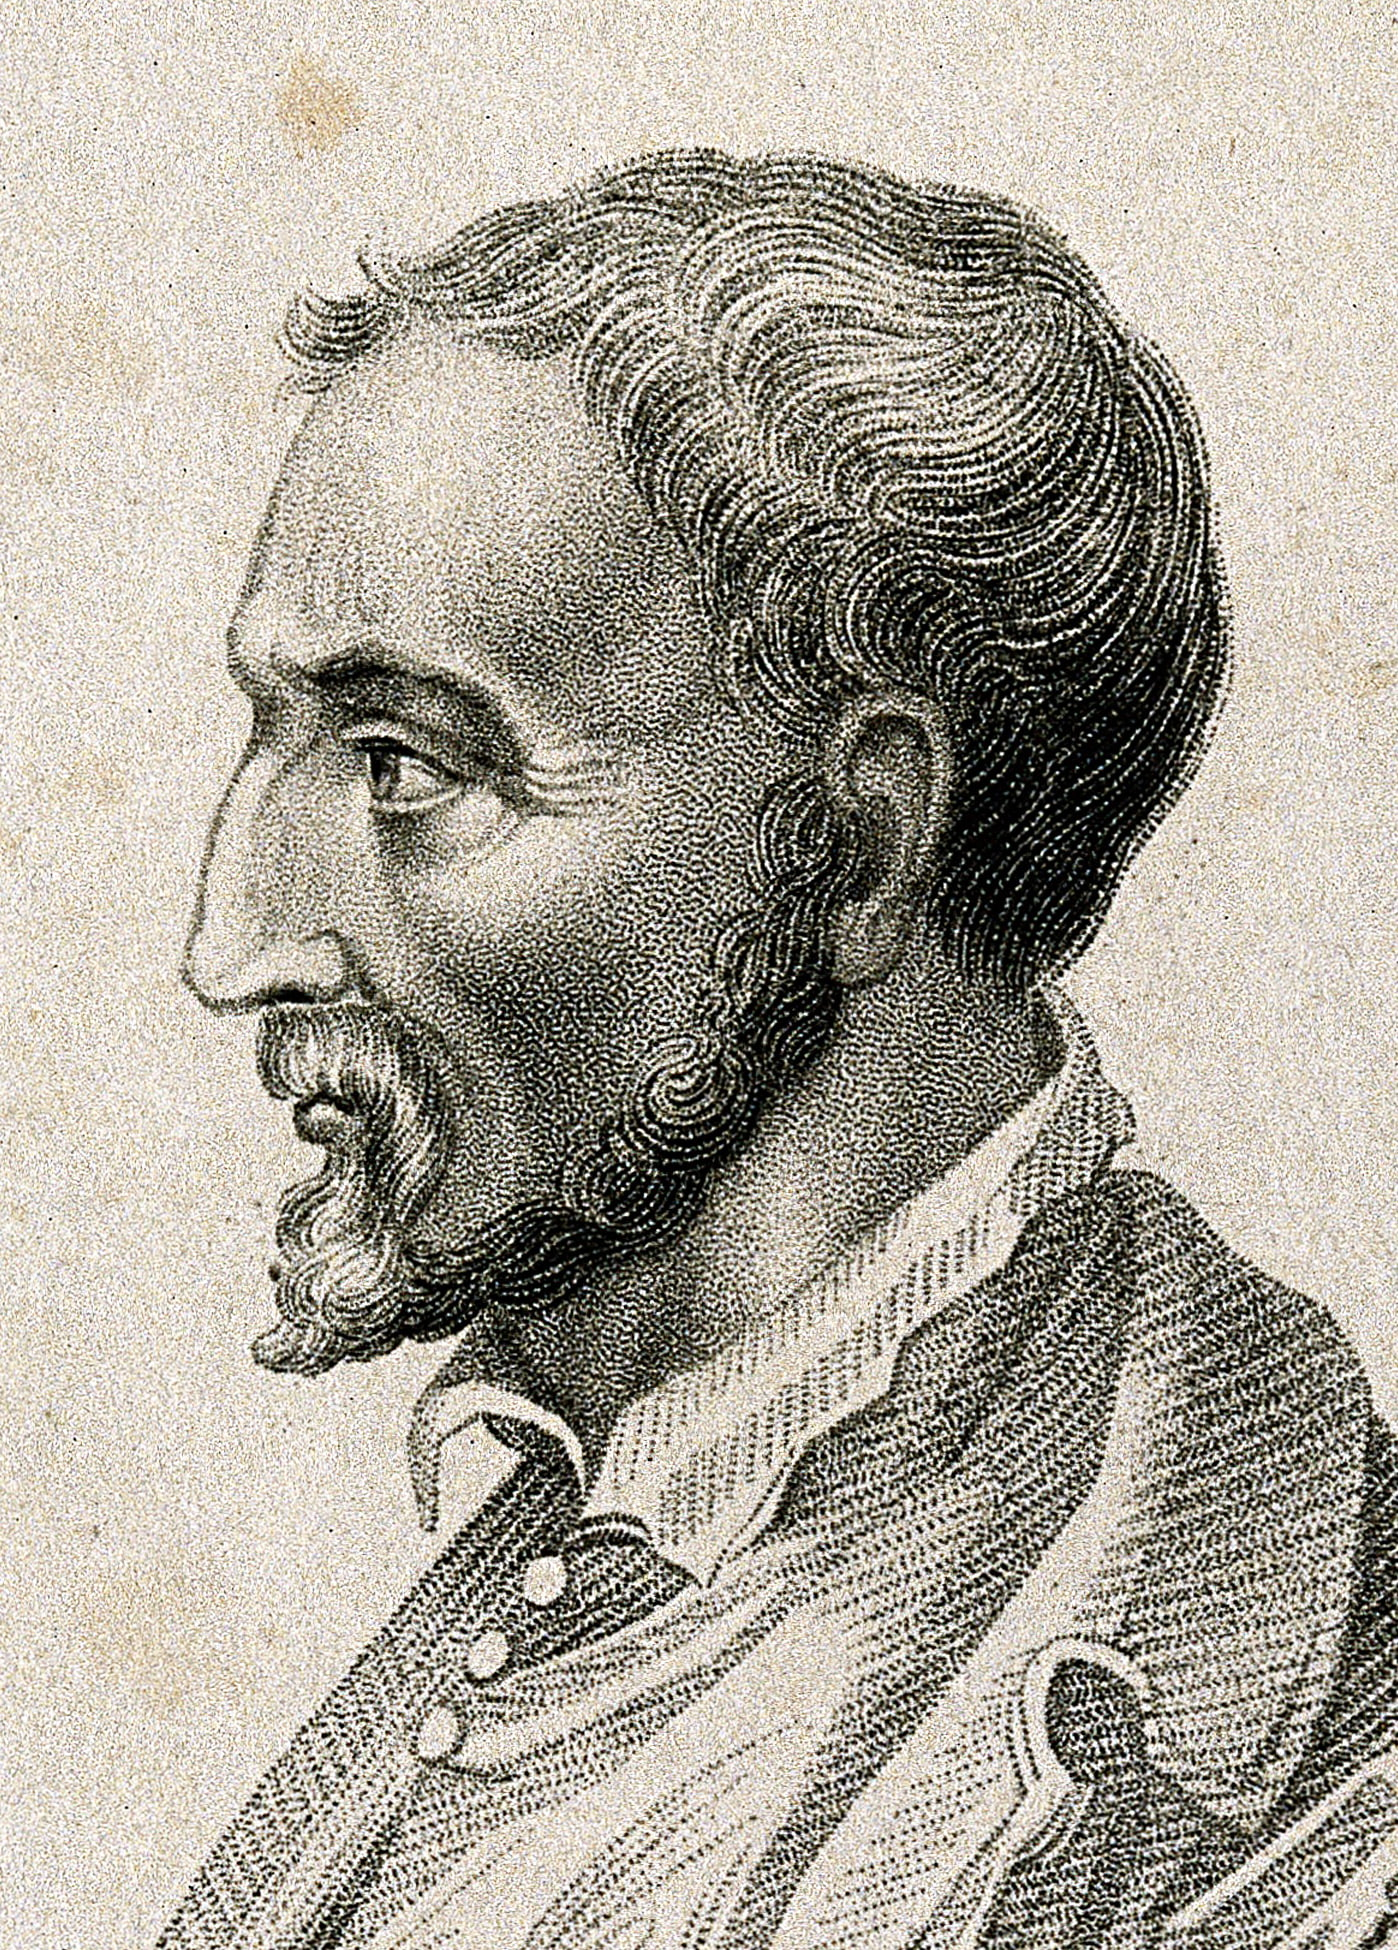
\includegraphics{images/jerome_cardan.jpg}
\end{marginfigure}

\textsl{
La théorie des équations polynomiales, qui précède de loin la définition formelle des polynômes, a été le propos essentiel de l'algèbre jusqu'au \textsc{xix}$^\me$ siècle. Elle est à l'origine de nombreuses notions: corps, nombres algébriques \dots Son développement est lié aux extensions successives de la notion de nombre: introduction des nombres négatifs, des nombres irrationnels, puis des nombres complexes. \\ 
Dès la plus haute Antiquité, on rencontre des exemples de résolutions d'équations. Les Babyloniens savent résoudre l'équation du second degré et les Grecs en font la base même de leur géométrie. \\
Après l'Antiquité, il faudra attendre le \textsc{xvi}$^\me$ siècle pour que des progrès substantiels apparaissent, dus à l'école italienne. \textsc{Scipone del Ferro}, \textsc{Tartaglia} et \textsc{Cardan} apportent la solution de l'équation du troisième dégré. L'équation générale est ramenée à la forme réduite $x^3 + px + q = 0$, dont une solution s'écrit
$$x = \sqrt[3]{-\frac{q}{2} + \sqrt{\frac{q^2}{4} + \frac{p^3}{27}}} + \sqrt[3]{-\frac{q}{2} - \sqrt{\frac{q^2}{4} + \frac{p^3}{27}}}.$$
Cette solution soulève des difficultés: si $\frac{q^2}{4} + \frac{p^3}{27}$ est négatif, cas où l'équation a des racines -- on le sait depuis \textsc{Archimède} -- on ne peut pas calculer $x$. Pour lever la difficulté, \textsc{Cardan} introduit timidement de nouveaux nombres, \say{ impossibles } ou \say{ imaginaires }. \textsc{Ferrari} et \textsc{Bombelli} résolvent l'équation du quatrième degré. \\
Grâce à l'école italienne, le théorie générale des équations algébriques se précise. L'équation étant mise sous le forme $P(x) = 0$, on prend conscience de l'importance du dégré de $P$ pour le nombre de solutions. On découvre que si $a$ est une racine de $P$, on peut factoriser par $x-a$. Les relations entre les coefficients et les fonctions symétriques des racines d'un polynôme apparaissent chez \textsc{Viète} (1540-1603), mais c'est \textsc{Girard} qui en 1629 leur donne toute leur extension. Suivi par \textsc{Newton}, il exprime les sommes des puissances des racines en fonction des coefficients. L'étude des fonctions symétriques des racines va se développer au \textsc{xvii}$^\me$ siècle avec \textsc{Waring} et au \textsc{xix}$^\me$ siècle avec \textsc{Cauchy}. \\
Au \textsc{xvii}$^\me$ siècle, la majorité des mathématiciens est convaincue qu'une équation de degré $n$ possède $n$ racines, celles-ci pouvant ne pas être réelles, mais il faut attendre \textsc{d'Alembert} pour trouver en 1724 une définition précise des nombres complexes (sous la forme $a + \sqrt{-1} b$). En 1799, \textsc{Gauss} fournit plusieurs preuves rigoureuses du \say{ théorème fondamental de l'algèbre } ou \say{ théorème de \textsc{d'Alembert}-\textsc{Gauss} }. \\
Des progrès sont réalisés également dans l'étude du nombre de racines réelles, et de leur signe. En 1637, \textsc{Descartes} énonce la règle qui porte son nom sur le nombre de racines positives d'un polynôme. On trouve dans \text{l'Algèbre} de \textsc{Rolle} (1690), la propriété suivante: entre deux solutions de l'équation $P(x)=0$, il existe au moins une solution de l'équation $P'(x)=0$. C'est \textsc{Sturm} qui formule, en 1829, les résultats les plus précis sur le nombre de racines réelles d'un polynôme. \\
Après les succès le l'école italienne au \textsc{xvi}$^\me$ siècle, les mathématiciens se sont attachés à trouver des formules analogues pour les dégrés suivants. Les réflexions sur cette question prennent un tour nouveau avec les travaux de \textsc{Lagrange} (1771), qui étudie les permutations des racines d'une équation laissant invariantes certaines fonctions de ces racines. Ces idées sont approfondies par \textsc{Cauchy} et \textsc{Ruffini}. \textsc{Abel} donne une démonstration rigoureuse de l'impossibilité de résoudre par radicaux l'équation générale de dégré $5$ en 1829. Enfin, en introduisant la notion de groupe, \textsc{Galois} énonce la condition générale à laquelle satisfait toute équation résoluble par radicaux (1831). \\
La distinction entre les nombres algébriques, racines d'un polynôme à coefficients entiers, et les autres qu'on nomme transcendants, date du \textsc{xvii}$^\me$ siècle, mais il faut attendre 1844 pour que \textsc{Liouville} démontre l'existence de nombres transcendants et plus longtemps encore pour que soit démontrée le trascendance de $\me$ (par \textsc{Hermite} en 1872) et celle de $\pi$ (par \textsc{Lindemann} en 1882). \\
Quant à la définition formelle des polynômes et à l'étude de leut structure, elles chemineront tout au long du \textsc{xix}$^\me$ siècle au rythme lent du processus d'axiomatisation de l'algèbre: par exemple, \textsc{Dedekind} introduit la notion de corps et définit les idéaux vers 1870.
}

\newpage

\section{Polynômes de \textsc{Legendre}}
\begin{tcolorbox}
    Pour tout $n \in \Ne$, on définit le polynôme $\Leg_n$ par:
    $$\Leg_n(X) = \frac{1}{2^n} \sum_{k=0}^{n} \binom{n}{k}^2 (X-1)^{n-k}(X+1)^{k},$$
    $$\Leg_n(X) = \frac{1}{2^n n!} \left( (X^2-1)^n \right)^{(n)}.$$
\end{tcolorbox}

Les polynômes de \textsc{Legendre} constituent l'exemple le plus simple d'une suite de polynômes orthogonaux. \\
La suite vient de \url{https://bibmath.net/dico/index.php?action=affiche&quoi=./l/legendrepoly.html}.
Les polynômes de \textsc{Legendre} sont orthogonaux pour le produit scalaire
$$\langle P, Q \rangle = \int_{-1}^1 P(t) Q(t) \d t$$
mais ne sont toutefois par orthonormaux car
$$\langle \Leg_n, \Leg_n \rangle = \frac{2}{2n+1}.$$

\begin{elem_sol}
    Pour montrer que $\Leg_n(X)$ est scindé à racines simples dans $]-1, 1[$, raisonner par récurrence et penser à \textsc{Rolle}. 
\end{elem_sol}

\begin{marginfigure}[-6cm]
	\begin{tikzpicture}
    \begin{axis}[width=6.5cm,
        axis lines=middle,
        inner axis line style={-latex},
        grid=major,
        xmin=-1.5, xmax=1.5,
        ymin=-1.5, ymax=1.5,
        % xlabel=$x$, xlabel style={right},
        % ylabel=$y$, ylabel style={above},
        tick style={thick},
        ticklabel style={font=\normalsize},
        xtick={-1, 0, 1}, 
        ytick={-1, 0, 1},
        % legend entries={0.5x},
            legend style={
            at={(1.05,0.4)},
            anchor=north,
            legend columns=1},
            legend cell align={left}
    ]
    
    \def\a{-1.1}
    \def\b{1.1}
    
    \addplot[blue,thick,samples=100,domain=\a:\b] {1};
    \addplot[red,thick,samples=100,domain=\a:\b] {x};
    \addplot[green,thick,samples=100,domain=\a:\b] {1/2*(3*x^2-1)};
    \addplot[violet,thick,samples=100,domain=\a:\b] {1/2*(5*x^3-3*x)};
    \addplot[black,thick,samples=100,domain=\a:\b] {1/8*(35*x^4-30*x^2+3)};
    \addplot[orange,thick,samples=100,domain=\a:\b] {1/8*(63*x^5-70*x^3+15*x)};
    
   % \legend{$\Leg_0$, 
   %         $\Leg_1$,
%            $\Leg_2$,
%            $\Leg_3$,
 %           $\Leg_4$,
  %          $\Leg_5$
   %         }
    \end{axis}
\end{tikzpicture}
	\caption{Les premiers polynômes de \textsc{Legendre}}
	{\scriptsize
	\color{blue} $\Leg_0 = 1$ \\ 
	\color{red} $\Leg_1 = x$ \\
	\color{green} $\Leg_2 = \frac{1}{2}(3x^2-1)$ \\
	\color{purple} $\Leg_3 = \frac{1}{2}(5x^3-3x)$ \\
	\color{black} $\Leg_4 = \frac{1}{8}(35x^4-30x^2+3)$ \\
	\color{orange} $\Leg_5 = \frac{1}{8}(63x^5-70x^3+15x)$
	}
\end{marginfigure}



\section{Polynômes de \textsc{Hilbert}}
\begin{defi}{Polynômes de \textsc{Hilbert}}
    On appelle famille des \emph{polynômes de \textsc{Hilbert}} la suite de polynômes $(\Hilb_n)_{n \in \N}$ définie par
    $$\Hilb_0 \defeq 1,\ \forall n \in \Ne,\ \Hilb_n \defeq \frac{X(X-1)\cdots(X-n+1)}{n!}.$$
\end{defi}

Voir aussi \nameref{polynome_hilbert} dans la partie algèbre linéaire. 

\begin{exercice}
    \marginnote[0cm]{Sources : \cite{exos_oraux} p.27, \cite{fmaalouf}}
    \begin{enumerate}
        \item Montrer que pour tout $n \in \N$, $\Hilb_n(\Z) \subset \Z$. En déduire que le produit de $n$ entiers consécutifs dans $\Z$ est divisible par $n!$.
        \item Soient $n \in \Ne$ et $Q \in \R_n[X]$. Montrer que les deux assertions suivantes sont équivalentes:
        \begin{enumerate}[label=(\roman*)]
            \item $Q(\Z) \subset \Z$,
            \item $\forall m \in \llbracket 0, n \rrbracket, Q(m) \in \Z$.
            \item $\exists (\lambda_0, \dots, \lambda_n) \in \Z^{n+1} \text{ tel que } Q = \sum\limits_{k=0}^n \lambda_k \Hilb_k$.
        \end{enumerate}
    \end{enumerate}
\end{exercice}

\begin{solution}
\end{solution}

\section{Polynômes de \textsc{Bernoulli}}
\marginnote[0cm]{Lire \cite{calcul_infinitesimal} p. 297}
% Note d'un thème (cf. bureau) \\

Il arrive fréquemment que le calcul exact d’une intégrale soit difficile, voire
impossible pour certaines fonctions et il est courant, dans ce cas, de chercher à
approcher la valeur de l’intégrale en utilisant des polynômes comme les polynômes de \nom{Bernoulli} par exemple.

\begin{defi}[Polynômes de \nom{Bernoulli}]
    Les \emph{polynômes de \nom{Bernoulli}} forment l'unique suite de polynômes $(\Bern_n)_{n \in \N}$ telle que:
    \begin{align*}
        &\Bern_0 = 1, \\
        \forall n \in \N,\ &\Bern'_{n+1} = (n+1)\Bern_n, \\
        \forall n \in \Ne,\ &\int_{0}^{1} \Bern_n(x) \d x = 0.
    \end{align*}
\end{defi}

\begin{defi}[Nombres de \nom{Bernoulli}]
    Pour tout $n \geqslant 0$, on pose $\mathrm{b}_n \defeq \Bern_n(0)$. La suite de réels $(\mathrm{b}_n)_{n \in \N}$ est appelée suite des \emph{nombres de \nom{Bernoulli}}.
\end{defi}  

\begin{table}[H]
    \centering
    \begingroup
        \renewcommand{\arraystretch}{1.2}
        \begin{tabularx}{\textwidth}{ |c| *{10}{>{\centering\arraybackslash}X|}}
         \hline
         $n$ & $0$ & $1$ & $2$ & $3$ & $4$ & $5$ & $6$ & $7$ & $8$ \\ \hline
         $\mathrm{b}_n$ & $1$ & $-\frac{1}{2}$ & $\frac{1}{6}$ & $0$ & $-\frac{1}{30}$ & $0$ & $\frac{1}{42}$ & $0$ & $-\frac{1}{30}$ \\
         \hline
    \end{tabularx}
    \endgroup
    \caption{Valeurs des premiers nombres de \textsc{Bernoulli}}
\end{table}

\begin{exercice}
    \begin{questions}
        \item Déterminer le degré de $\Bern_n(X)$ pour $n \geqslant 0$. 
        \item Montrer que, pour tout $n \geqslant 2$, $\Bern_n(0) = \Bern_n(1)$.
        \item Soient $n \in \N$ et $x \in \R$. Montrer que 
        $$\Bern_n(x) = \sum_{k=0}^n \binom{n}{k} \mathrm{b}_{n-k} x^k.$$
        \item En déduire, pour $n \geqslant 1$, une expression de $\mathrm{b}_n$ en fonction de $\mathrm{b}_0, \dots, \mathrm{b}_{n-1}$.
        \item Montrer que la suite $(\mathrm{b}_n)_{n \in \N}$ est une suite de rationnels et que, pour $n \geqslant 0$, les polynômes $\Bern_n(X)$ sont à coefficients rationnels.
        \item Montrer que pour tout $n \geqslant 0$, $(-1)^n \Bern_n(1-X) = \Bern_n(X)$.
        \item En déduire que 
        $$
        \begin{cases}
            \forall n \geqslant 1, \mathrm{b}_{2n+1} = 0, \\
            \forall n \geqslant 0, \Bern_{2n+1}(\frac{1}{2}) = 0.
        \end{cases}
        $$
    \end{questions}    
\end{exercice}

\section{Polynômes de \textsc{Tchebychev}}
\begin{defi}{Polynômes de \textsc{Tchebychev}}
    Les polynômes de \textsc{Tchebychev} de première espèce sont les uniques polynômes $(\Tcheby_n)_{n \geqslant 0}$ définis sur $]-1, 1[$ par
    $$\forall \theta \in \R,\ \Tcheby_n (\cos \theta) = \cos(n \theta).$$
\end{defi}

Vérifions tout d'abord qu'une telle suite existe bien et qu'elle est unique.

\begin{marginfigure}[-4.5cm]
    \centering
	\begin{tikzpicture}
    \begin{axis}[width=6.5cm,
        axis lines=middle,
        inner axis line style={-latex},
        grid=major,
        xmin=-1.5, xmax=1.5,
        ymin=-1.5, ymax=1.5,
        % xlabel=$x$, xlabel style={right},
        % ylabel=$y$, ylabel style={above},
        tick style={thick},
        ticklabel style={font=\normalsize},
        xtick={-1, 0, 1}, 
        ytick={-1, 0, 1},
        % legend entries={0.5x},
            legend style={
            at={(1.05,0.4)},
            anchor=north,
            legend columns=1},
            legend cell align={left}
    ]
    
    \def\a{-1.1}
    \def\b{1.1}
    
    \addplot[blue,thick,samples=100,domain=\a:\b] {1};
    \addplot[red,thick,samples=100,domain=\a:\b] {x};
    \addplot[green,thick,samples=100,domain=\a:\b] {2*x^2-1};
    \addplot[violet,thick,samples=100,domain=\a:\b] {4*x^3-3*x};
    \addplot[black,thick,samples=100,domain=\a:\b] {8*x^4-8*x^2+1};
    \addplot[orange,thick,samples=100,domain=\a:\b] {16*x^5-20*x^3+5*x};
    
   % \legend{$\Leg_0$, 
   %         $\Leg_1$,
%            $\Leg_2$,
%            $\Leg_3$,
 %           $\Leg_4$,
  %          $\Leg_5$
   %         }
    \end{axis}
\end{tikzpicture}
	\caption*{\centering Polynômes de \textsc{Tchebychev} de première espèce}
	\begin{align*}
	   	\color{blue} \Tcheby_0 = 1 \\
    	\color{red} \Tcheby_1 = x \\
    	\color{green} \Tcheby_2 = 2x^2-1 \\
    	\color{purple} \Tcheby_3 = 4x^3-3x \\
    	\color{black} \Tcheby_4 = 8x^4-8x^2+1 \\
    	\color{orange} \Tcheby_5 = 16x^5-20x^3+5x
	\end{align*}
\end{marginfigure}

\begin{preuve}
    \begin{description}
        \item[Existence] Nous allons montrer que la suite $(\Tcheby_n)_{n \geqslant 0}$ vérifie une relation de récurrence. \\
        Soit $n \in \N$,
        \begin{align*}
            \Tcheby_{n+2}(\cos \theta) &= \cos((n+2) \theta) \\
            &= \cos((n+1) \theta) \cos(\theta) - \sin((n+1) \theta) \sin(\theta) \\
            &= \Tcheby_{n+1}(\cos \theta) \cos(\theta) - \frac{1}{2} \left(\cos(n \theta) - \cos((n+2)\theta)\right) \\
            \Tcheby_{n+2}(\cos \theta) &= \Tcheby_{n+1}(\cos \theta) \cos(\theta) - \frac{1}{2} \Tcheby_n(\cos \theta) + \frac{1}{2} \Tcheby_{n+2}(\cos \theta)
        \end{align*}
        d'où
        $$\Tcheby_{n+2} = 2X \Tcheby_{n+1} - \Tcheby_n.$$
        \item[Unicité] L'unicité de $\Tcheby_n$ pour $n$ fixé est garantie pas l'identification de \ptnclegras{deux polynômes coïncidant} sur $]-1, 1[$. 
    \end{description}
\end{preuve}

\marginnote[-6cm]{
    \begin{kaobox}[frametitle=Formule de trigonométrie]
        $$\sin a \sin b = \frac{1}{2} \big( \cos(a-b) - \cos(a+b) \big)$$
    \end{kaobox}
}

\begin{exercice}
    Soit $n \in \N$, déterminer une expression de $\Tcheby_n$.
\end{exercice}  

\begin{solution}
    \begin{align*}
        \cos(n \theta) &= \Reel \left( \me^{\mi n \theta}) = \Reel((\cos \theta + \mi \sin \theta)^n \right)\\
        &= \Reel\left( \sum_{k=0}^n \binom{n}{k} (\cos\theta)^k (\mi \sin\theta)^{n-k} \right) \\
        &= ...
    \end{align*}
    $$\forall n \in \N,\ \Tcheby_n = \sum_{k=0}^{\lfloor n / 2 \rfloor} (-1)^k \binom{n}{2k} X^{n-2k} (1-X^2)^k.$$
\end{solution}

\begin{prop}{}
    \begin{enumerate}
        \item $$\deg \Tcheby_n = n \text{ et } \mathrm{cd}\, \Tcheby_n = 2^{n-1}$$
        \item $\Tcheby_n$ est pair si $n$ est pair et vice versa. \\
        \item Pour tout $n, m$, $\Tcheby_n \circ \Tcheby_m = \Tcheby_{nm}$. \\
        \item $$(1-x^2) \Tcheby''_n(x) - x \Tcheby'_n(x) + n^2 \Tcheby_n(x) = 0.$$
        \item $\Tcheby_n$ admet $n$ racines simples qui sont
        $$a_{k,n} = \cos \left( \frac{(2k-1) \pi}{2n}\right),\ k \in \llbracket 1, n \rrbracket.$$
        \item Sur $[-1, 1]$, $\Tcheby_n$ admet $n+1$ extrema égaux à $1$ en les points
        $$b_{k,n} = \cos\left( \frac{k \pi}{n} \right),\ k \in \llbracket 0, n \rrbracket.$$
    \end{enumerate}
\end{prop}

\begin{preuve}
    \begin{enumerate}
        \item ff
        \item ff
        \item 
    \end{enumerate}
\end{preuve}



\section{Polynômes scindés}
\begin{exercice}
    \marginnote[0cm]{Source : \cite{exos_oraux} p. 23}
    Soient $Q \in \R[X]$ et $a \in \R$. On suppose que $Q$ est scindé sur $\R[X]$, montrer que $Q'+aQ$ l'est aussi. 
\end{exercice}

\begin{elem_sol}
    Si $a=0$, appliquer le \ptnclegras{théorème de \textsc{Rolle}} sur chacun des intervalles $[x_i, x_{i+1}]$ où $x_i$ et $x_{i+1}$ sont deux racines réelles consécutives de $Q$.
    \begin{enumerate} 
        \item Poser $\varphi:t \mapsto \exp(at)Q(t)$.
        \item Démarche à revoir.
    \end{enumerate}
\end{elem_sol}

\chapter{Algèbre linéaire, Matrices}
\labch{algebre_lineaire_matrices}

\textsl{Au \textsc{xviii}$^\me$ siècle se développent la résolution des systèmes linéaires et la théorie des déterminants. Les raisonnements suggèrent rapidement le concept d'espace à $n$ dimensions. Mais il fallait oser un langage géométrique, alors qu'une interprétation sensible dans le plan ou l'espace faisait défaut pour $n > 3$. \\
De manière indépendante, \textsc{Cayley} en Angleterre et \textsc{Grassman} en Allemagne franchissent le pas vers 1843-1845 et parlent d'espace à $n$ dimensions. Le point de vue de \textsc{Cayley} est issu directement de la géométrie analytique: un vecteur d'un espace à $n$ dimensions est un système de $n$ réels ou $n$ complexes. L'addition de deux vecteurs et la multiplication par un scalaire sont naturellement introduites par la généralisation de la dimension $3$. Pour parvenir vraiment à la notion d'espace vectoriel, il faut dégager le concept de sous-espace et de dimension d'un sous-espace. C'est ce que fera \textsc{Grassman} (professeur de lycée autodidacte en marge des milieux de la recherche) en cherchant à développer une analyse géométrique portant sur des calculs intrinsèques indépendants du choix des coordonnées. \textsc{Grassman} introduit le produit extérieur de deux vecteurs, la définition de l'indépendance linéaire, de la dimension d'un espace et démontre la relation fondementale
$$\dim V + \dim W = \dim (V + W) + \dim V \cap W.$$
Ces travaux eurent peu d'impact au début, mais ils furent repris par Henri \textsc{Poincaré} et Élie \textsc{Cartan} (notamment son \say{algèbre extérieure} en géométrie différentielle). \\
C'est en 1888 que \textsc{Peano} donnera la définition axiomatique d'un espace vectoriel réel. Jusqu'en 1930, le point de vue des matrices et des coordonnées prédomine par rapport au point de vue intrinsèque des espaces vectoriels.
}

\begin{marginfigure}[-13cm]
    \centering
    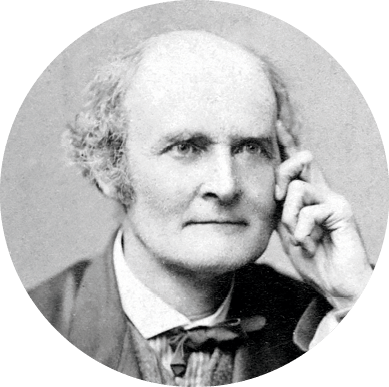
\includegraphics{images/arthur_cayley.png}
    \caption*{\centering Arthur \textsc{Cayley} (1821-1895)}
\end{marginfigure}

\begin{marginfigure}[-6cm]
    \centering
    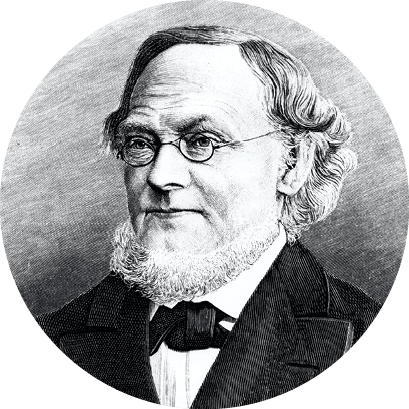
\includegraphics{images/hermann_grassmann.png}
    \caption*{\centering Hermann \textsc{Grassmann} (1809-1877)}
\end{marginfigure}

\newpage

% \section{Cours: changement de base}
% \begin{marginfigure}
%     \tikzset{>=latex} % for LaTeX arrow head
\colorlet{xcol}{blue!70!black}
\tikzstyle{rvec}=[->,thick,xcol,line cap=round]

% VECTOR breakdown on axis
\begin{tikzpicture}
  \small
  \def\L{0.8}
  \def\R{2.3}
  \def\ang{26}
  \def\thet{-52}
  \coordinate (O) at (0,0);
  \coordinate (O1) at (3.6,0.4);
  \coordinate (O2) at (0.9,1.8);
  \coordinate (O3) at (1.8,-0.5);
  \coordinate (R) at (\ang:\R);
  \node[fill=black,circle,inner sep=0.9] (R') at (R) {};
  
  % O1
  \draw[<->,thick] (\L,0) node[below] {$x$} --
                   (O) node[below left=-3] {O} --
                   (0,\L) node[left=-1] {$y$};
  \draw[rvec] (O) -- (R');
  
  % O1
  \begin{scope}[shift={(O1)}]
    \draw[<->,thick] (\L,0) node[below=-2] {$x'$} --
                     (0,0) node[below left=-2] {O$'$} --
                     (0,\L) node[left=-2] {$y'$};
    \draw[rvec] (0,0) -- (R');
  \end{scope}
  
  % O2
  \begin{scope}[shift={(O2)}]
    \draw[<->,thick] (\L,0) node[above] {$x''$} --
                     (0,0) node[above left=-4] {O$''$} --
                     (0,-\L) node[left] {$y''$};
    \draw[rvec] (0,0) -- (R');
  \end{scope}
  
  % O3
  \begin{scope}[shift={(O3)}]
    \draw[<->,thick] (\thet:\L) node[below left=-2] {$x'''$} --
                     (0,0) node[left=-2] {O$'''$} --
                     (\thet+90:\L) node[above=-2] {$y'''$};
    \draw[rvec] (0,0) -- (R');
  \end{scope}
  
\end{tikzpicture}
% \end{marginfigure}

\section{Polynômes de \textsc{Hilbert}} \label{polynome_hilbert}
\begin{tcolorbox}
    On appelle famille des polynômes de \textsc{Hilbert} la suite de polynômes $(\Hilb_n)$ définie par
    $$\Hilb_0(X) = 1,\ \forall n \in \Ne,\ \Hilb_n = \frac{X(X-1)\dots(X-n+1)}{n!}.$$
    La famille $(\Hilb_0, \dots, \Hilb_n)$ forme une base de $\C_n[X]$.
\end{tcolorbox}

\section{Matrice de \textsc{Vandermonde}} %%%%%%%%%%%%%%%%%%%%%%%%%%%%
\begin{defi}[Matrice de \nom{Vandermonde}]
    Soit $(\alpha_1, \dots, \alpha_n)$ une famille de complexes. On définit la \emph{matrice de \nom{Vandermonde}} de la famille $(\alpha_1, \dots, \alpha_n)$ par
    $$\Vandermonde(\alpha_1, \dots, \alpha_n) \defeq \begin{pmatrix}
    1 & \alpha_1 & \alpha_1^2 & \cdots & \alpha_1^{n-1} \\
    \vdots & \vdots & \vdots & \ddots & \vdots \\
    1 & \alpha_n & \alpha_n^2 & \cdots & \alpha_n^{n-1}
    \end{pmatrix}.$$
    On considère ici une matrice de \nom{Vandermonde} carrée.
\end{defi}

\newcommand{\vandk}{
\left(\begin{gathered}
    [every node/.style={anchor=south west}]
        \node[mitikzpicturenimum width=2cm,minimum height=1.5cm] at (-0.16,0.625) {$\Vandermonde(\alpha_1, \dots, \alpha_{k-1})$};
        \node[minimum width=0.5cm,minimum height=0.5cm] at (0,0.05) {$1$};
        \node[minimum width=0.5cm,minimum height=0.5cm] at (0.4, 0) {$\alpha_{k}$};
        \node[minimum width=0.5cm,minimum height=0.5cm] at (0.95,0) {$\cdots$};
        \node[minimum width=0.5cm,minimum height=0.5cm] at (1.5,0) {$\alpha_{k}^{k-2}$};
        \node[minimum width=1cm,minimum height=0.5cm] at (2.5,0) {$\alpha_{k}^{k-1}$};
        \node[minimum width=1cm,minimum height=1cm] at (2.5,0.4) {$\alpha_{k-1}^{k-1}$};
        \node[minimum width=1cm,minimum height=1cm] at (2.5,1) {$\vdots$};
        \node[minimum width=1cm,minimum height=1cm] at (2.5,1.4) {$\alpha_1^{k-1}$};
        \draw (0,0.6) -- (2.5,0.6);
        \draw (2.5,0.6) -- (2.5,2.225);
        \draw[dashed] (2.5,0.6) -- (3.5,0.6);
        \draw[dashed] (2.5,0.6) -- (2.5,0);
    \endtikzpicture
    \end{gathered}\right)
}

\begin{remarque}
    Soit $(\alpha_1, \dots, \alpha_n)$ une famille de complexes. Les matrices de \nom{Vandermonde} des familles $(\alpha_1, \dots, \alpha_k)$ pour $2 \leqslant k \leqslant n$ sont imbriquées les unes dans les autres de la manière suivante
    $$\Vandermonde(\alpha_1, \dots, \alpha_k) = ....$$
\end{remarque}

\begin{prop}[Déterminant de \nom{Vandermonde}]\labprop{determinant_vandermonde}
    $$\det \big( \Vandermonde(\alpha_1, \dots, \alpha_n) \big) = \smashoperator{\prod_{1\leqslant i < j \leqslant n}}(\alpha_j - \alpha_i).$$
\end{prop}

\newcommand{\detvandnplusun}{
\left|\begin{gathered}
    \tikzpicture[every node/.style={anchor=south west}]
        \node[minimum width=2cm,minimum height=1.5cm] at (0.05,0.625) {$\Vandermonde(\alpha_1, \dots, \alpha_{n})$};
        \node[minimum width=0.5cm,minimum height=0.5cm] at (0,0.05) {$1$};
        \node[minimum width=0.5cm,minimum height=0.5cm] at (0.3, 0) {$\alpha_{n+1}$};
        \node[minimum width=0.5cm,minimum height=0.5cm] at (1.05,0) {$\cdots$};
        \node[minimum width=0.5cm,minimum height=0.5cm] at (1.5,0) {$\alpha_{n+1}^{n-1}$};
        \node[minimum width=1cm,minimum height=0.5cm] at (2.5,0) {$\alpha_{n+1}^{n}$};
        \node[minimum width=1cm,minimum height=1cm] at (2.5,0.4) {$\alpha_{n}^{n}$};
        \node[minimum width=1cm,minimum height=1cm] at (2.5,1) {$\vdots$};
        \node[minimum width=1cm,minimum height=1cm] at (2.5,1.4) {$\alpha_1^{n}$};
        \draw (0,0.6) -- (2.5,0.6);
        \draw (2.5,0.6) -- (2.5,2.225);
        \draw[dashed] (2.5,0.6) -- (3.5,0.6);
        \draw[dashed] (2.5,0.6) -- (2.5,0);
    \endtikzpicture
    \end{gathered}\right|
}


\begin{demo}
    Nous allons raisonner par récurrence sur la taille de la matrice. Pour tout $n \in \Ne$ on pose
    $$\mathscr{P}_n: \text{\say{ Soit $(\alpha_1, \dots, \alpha_n) \in \C^n$, $\det \big(\Vandermonde(\alpha_1, \dots, \alpha_n)\big) = \smashoperator{\prod\limits_{1\leqslant i < j \leqslant n}}(\alpha_j - \alpha_i)$}}.$$
    \begin{itemize}
        \item[$\rhd$] L'initialisation pour $n = 1$ est triviale.
        \item[$\rhd$] Soit $n \in \Ne$. On suppose $\mathscr{P}_n$ vraie, montrons $\mathscr{P}_{n+1}$. \\ 
        Soit $(\alpha_1, \dots, \alpha_n, \alpha_{n+1})$ une famille de complexes. \\
        On pose $P(X) \defeq \prod\limits_{j=1}^n (X-\alpha_j) \defeq X^n + \sum\limits_{k=0}^{n-1} p_k X^k$. \\
        D'après les propriétés du déterminant, en ajoutant les $n$ premières colonnes respectivement multipliée par $p_k$ à la dernière, on obtient
        \begin{align*}
            \detvandnplusun &= \\
            &= \\
            &= \det \big( \Vandermonde(\alpha_1, \dots, \alpha_n) \big) P(\alpha_{n+1}) \\
            \text{par hypothèse de récurrence } &= \smashoperator{\prod\limits_{1\leqslant i < j \leqslant n}}(\alpha_j - \alpha_i) \times \prod\limits_{j=1}^n (\alpha_{n+1}-\alpha_j) \\
            \det \big( \Vandermonde(\alpha_1, \dots, \alpha_{n+1}) \big) &= \smashoperator{\prod_{1\leqslant i < j \leqslant n + 1}}(\alpha_j - \alpha_i).
        \end{align*}
        La proprité est donc vraie au rang $n+1$ et on en déduit par récurrence qu'elle est vraie pour tout $n \in \Ne$.
    \end{itemize}
\end{demo}

\begin{corol}
    La famille $(\alpha_1, \dots, \alpha_n)$ est libre si et seulement si le déterminant de sa matrice de \textsc{Vandermonde} est non nul.
\end{corol}

\begin{demo} 
    D'après la \refprop{determinant_vandermonde}, la matrice de \nom{Vandermonde} de la famille $(\alpha_1, \dots, \alpha_n)$ est inversible si et seulement si les $\alpha_i$ sont distincts deux à deux. 
\end{demo}

\begin{exercice}
    \source{\cite{maths-france} Planche no 35. Déterminants}
    Pour $a \in \C$, on pose pour tout $x \in \R$, $f_a(x) \defeq \e^{ax}$. Soit $(a_1, \dots, a_n)$, $n$ complexes deux à deux distincts. Montrer que la famille de fonctions $(f_{a_k})_{1 \leqslant k \leqslant n}$ est libre.
\end{exercice}

\begin{solution}
    \item Soit $(\lambda_k)_{1 \leqslant k \leqslant n} \in \C^n$ tel que $\sum\limits_{k=1}^n \lambda_k f_{a_k} = 0$. Alors, 
    \begin{align*}
        & \forall p \in \llbracket 0, n-1 \rrbracket, \sum_{k=1}^n \lambda_k f^{(p)}_{a_k} = 0, \\
        \text{soit } & \forall p \in \llbracket 0, n-1 \rrbracket, \forall x \in \R, \sum_{k=1}^n \lambda_k a_k^p \e^{a_k x} = 0, \\
        \text{pour $x=0$ } & \forall p \in \llbracket 0, n-1 \rrbracket, \sum_{k=1}^n \lambda_k a_k^p = 0.
    \end{align*}
    Les $n$ dernières égalités écrites constituent un système $(\mathscr{S})$ de $n$ équations linéaires à $n$ inconnues $\lambda_1, \dots, \lambda_n$. Le déterminant de ce système est $\Vandermonde(a_1, \dots, a_n)$ et ce déterminant est non nul car les $a_k$ sont deux à deux distincts. Par suite, $(\mathscr{S})$ est un système de \nom{Cramer} homogène. Le système $(\mathscr{S})$ admet donc l'unique solution $(\lambda_1, \dots, \lambda_n) = (0, \dots, 0)$ et on a ainsi montré la liberté de la famille $(f_{a_k})_{1 \leqslant k \leqslant n}$.
\end{solution}

\subsection{Inverse de la matrice de {\nom{Vandermonde}}}

\begin{exercice}
    \source{\cite{exos_oraux} p.81}
    Soient $n \in \Ne$ et $(x_1, \dots, x_n)$ des complexes deux à deux distincts.
    \begin{enumerate}
        \item Montrer que l'application
        $$
        \fonction[\varphi]{\C_{n-1}[X]}{\C^n}{P}{\big( P(x_1), \dots, P(x_n) \big)}
        $$
        est un isomorphisme. Montrer que sa matrice dans les bases canoniques de départ et d'arrivée est 
        $$
        M_n(x_1, \dots, x_n) \defeq
        \begin{pmatrix}
            1 & x_1 & x_1^2 & \cdots & x_1^{n-1} \\
            1 & x_2 & x_2^2 & \cdots & x_2^{n-1} \\
            \vdots & \vdots & \vdots & & \vdots \\
            1 & x_n & x_n^2 & \cdots & x_n^{n-1}
        \end{pmatrix}.
        $$
        \item On note $\Lag_1(X), \dots, \Lag_n(X)$ les polynômes interpolateurs de \textsc{Lagrange} associés à $x_1, \dots, x_n$. Donner une relation entre les coefficients de $\Inv{M_n(x_1, \dots, x_n)}$ et ceux des polynômes $\Lag_i(X)$.
    \end{enumerate}
\end{exercice}


\section{Polynômes de \textsc{Lagrange}} 
\marginnote[0cm]{\url{https://perso.math.univ-toulouse.fr/fdelebec/files/2018/03/chap01-L2.pdf}}
\subsection{Motivations de l'interpolation polynomiale}
En analyse numérique, une fonction $f$ inconnue explicitement est souvent connue seulement en certains points $x_0, \dots, x_d$, ou évaluable uniquement au moyen de l'appel à un code coûteux. \\
Mais dans de nombreux cas, on a besoin d'effectuer des opérations (dérivation, intégration, \dots) sur la fonction $f$. \\
On cherche donc à reconstruire cette fonction $f$ par une autre fonction $f_r$ simple et facile à évaluer à partir des données discrètes de $f$. On espère que le modèle $f_r$ ne sera pas trop éloigné de la fonction $f$ aux autres points.
\begin{center}
    Pourquoi utiliser des polynômes pour reconstruire la fonction $f$ ?    
\end{center}
\marginnote[0cm]{\note cf. p. [...]}
\begin{itemize}
    \item \textbf{Le théorème d'approximation de \textsc{Weierstrass}:} \note \\
    pour toute fonction $f$ définie et continue sur un intervalle $[a, b]$ et pour tout $\varepsilon > 0$, il existe un polynôme $P$ tel que 
    $$\forall x \in [a, b],\ |f(x) - P(x)| < \varepsilon.$$
    Plus $\varepsilon$ est petit, plus le degré du polynôme est grand.
    \item \textbf{La simplicité de l'évaluation d'un polynôme par le schéma de \textsc{Hörner}:}
    $$\sum_{j=0}^n c_j x^j = \Big( \cdots \big( (c_n x + c_{n-1})x + c_{n-2} \big)x + \cdots c_1 \Big)x + c_0.$$
\end{itemize}

\begin{marginfigure}[-1cm]
    \centering
    \begin{tikzpicture}
    \begin{axis}[width=6.5cm,
        axis lines=middle,
        grid=major,
        xmin=-1.2, xmax=1.2,
        ymin=-1.1, ymax=1.1,
        % xlabel=$x$, xlabel style={right},
        % ylabel=$y$, ylabel style={above},
        %tick style={thick},
        %ticklabel style={font=\normalsize},
        xtick=\empty, 
        ytick=\empty,
        axis line style={-latex}
    ]
    
    \def\a{-1.1}
    \def\b{1.1}
    \def\colour{BrickRed}
    
    \addplot[red,thick,samples=100,domain=\a:\b] {
    (x+5/8)*(x-1/8)*(x-1/2)*(x-4/5)/((-7/8+5/8)*(-7/8-1/8)*(-7/8-1/2)*(-7/8-4/5))*(-1/2)
    + (x+7/8)*(x-1/8)*(x-1/2)*(x-4/5)/((-5/8+7/8)*(-5/8-1/8)*(-5/8-1/2)*(-5/8-4/5))*(-1/9)
    + (x+7/8)*(x+5/8)*(x-1/2)*(x-4/5)/((1/8+7/8)*(1/8+5/8)*(1/8-1/2)*(1/8-4/5))*(-1/8)
    + (x+7/8)*(x+5/8)*(x-1/8)*(x-4/5)/((1/2+7/8)*(1/2+5/8)*(1/2-1/8)*(1/2-4/5))*(1/2)
    + (x+7/8)*(x+5/8)*(x-1/8)*(x-1/2)/((4/5+7/8)*(4/5+5/8)*(4/5-1/8)*(4/5-1/2))*(2/9)
    };
    
    \addplot[\colour,mark=*] coordinates {(-7/8,-1/2)} node[left] {$M_0$};
    \addplot[\colour,mark=*] coordinates {(-5/8,-1/9)} node[below] {$M_1$};
    \addplot[\colour,mark=*] coordinates {(1/8,-1/8)} node[below] {\contour{white}{$M_2$}};
    \addplot[\colour,mark=*] coordinates {(1/2,1/2)} node[above] {\contour{white}{$M_3$}};
    \addplot[\colour,mark=*] coordinates {(4/5,2/9)} node[right] {$M_4$};
    
    \draw[blue, thick, dotted] (-7/8,-1/2) -- (-7/8, 0);
    \draw[blue, thick, dotted] (-7/8,-1/2) -- (0, -1/2);

    \draw[blue, thick, dotted] (-5/8,-1/9) -- (-5/8, 0);
    \draw[blue, thick, dotted] (-5/8,-1/9) -- (0, -1/9);

    \draw[blue, thick, dotted] (1/8,-1/8) -- (1/8, 0);
    \draw[blue, thick, dotted] (1/8,-1/8) -- (0,-1/8);

    \draw[blue, thick, dotted] (1/2,1/2) -- (1/2, 0) node[below] {$a_3$};
    \draw[blue, thick, dotted] (1/2,1/2) -- (0, 1/2) node[left] {$f_3$};
    
    \draw[blue, thick, dotted] (4/5,2/9) -- (4/5, 0);
    \draw[blue, thick, dotted] (4/5,2/9) -- (0, 2/9);
    
    \draw[black, thick] (-0.8,0.5) node[above] 
    {\footnotesize \contour{white}{{\parbox{2cm}{\centering Polynôme \\ interpolateur}}}} to [out=640,in=800] ($(-0.3,-1/4)$);
    \end{axis}
    
\end{tikzpicture}
\end{marginfigure}

Plus précisément, étant donnés $d+1$ points d'abscisses distinctes $M_i \defeq (a_i, f_i)$ pour $i \in \llbracket 0, d \rrbracket$ dans le plan, le problème de l'interpolation polynomiale consiste à trouver un polynôme de degré inférieur ou égal à $m$ dont le graphe passe par les $d+1$ points $M_i$.\\

\subsection{Interpolation lagrangienne}

Les polynômes de \textsc{Lagrange} permettent d'interpoler une série de $n+1$ points par un polynôme de degré $n$ qui passe exactement par ces points.

\begin{theo}{Propriété fondamentale des polynômes de \textsc{Lagrange}}
    Soient $n \in \N$ et $(x_0, \dots, x_n)$ des complexes deux à deux distincts. \\
    Pour tout $i \in \llbracket 0, n \rrbracket$, il existe un unique polynôme $\Lag_i \in \C_n[X]$ tel que 
    \begin{equation} \label{prop_fondamentale}
        \forall j \in \llbracket 0, n \rrbracket,\ \Lag_i(x_j) = \delta_{i,j}.\ \note
    \end{equation}
\end{theo}

\marginnote[-4cm]{
    \begin{defi}{\note Symbole de \textsc{Kronecker}}
    $$
    \delta_{i,j} \defeq \begin{cases}
    1 \quad \text{ si } i=j, \\
    0 \quad \text{ si } i \not= j.
    \end{cases}
    $$
    \end{defi}
}

\begin{preuve}
    \marginnote[0cm]{\url{https://www.youtube.com/watch?v=blB2SAYpobA}}
    On considère $n + 1$ complexes deux à deux distincts, notés $x_0, \dots, x_n$.
    \begin{alignat*}{2}
        \text{Soit } \varphi\ :\ \R_n[X]\ &\longrightarrow\ \R^{n+1}\\
        P\ &\longmapsto\ \big(P(x_0), \dots, P(x_n) \big).
    \end{alignat*}
    \begin{itemize}
        \item[$\rhd$] Soit $P \in \Ker \varphi$. Alors le polynôme $P$ a $n+1$ racines discintes. Or il est de degré inférieur à $n$ donc est le polynôme nul. On en déduit que $\varphi$ est injective ce qui assure l'\ptnclegras{unicité} des polynômes interpolateurs de \textsc{Lagrange}.
        \item[$\rhd$] Comme $\dim \R_n[X] = \dim \R^{n+1}$ et que l'application $\varphi$ est injective, c'est un isomorphisme \note.
        \item[$\rhd$] En particulier, l'application $\varphi$ est surjective ce qui assure l'\ptnclegras{existence} de ces polynômes. 
    \end{itemize}
    \marginnote[-4cm]{
        \begin{prop}{}
            \note Si $f$ est une application linéaire d'un espace de dimension finie $E$ dans un espace de dimension finie $F$ avec $\dim E = \dim F$, il suffit que $f$ soit injective ou surjective pour que $f$ soit un isomorphisme.
        \end{prop}
    }
\end{preuve}

\begin{defi}{Polynômes de \textsc{Lagrange}}
    Soient $n \in \N$ et $(x_0, \dots, x_n)$ des complexes deux à deux distincts. On appelle famille des \emph{polynômes de \textsc{Lagrange}} la suite de polynômes $(\Lag_n)_{n \in \N}$ vérifiant la relation (\ref{prop_fondamentale}).
\end{defi}

\begin{remarque}
    Une famille de polynômes de \textsc{Lagrange} est définie à partir d'une famille de complexes deux à deux distincts. 
\end{remarque}

\begin{prop}{Expression des polynômes de \textsc{Lagrange}}
    Soient $n \in \N$ et $(x_0, \dots, x_n)$ des complexes deux à deux distincts. Les polynômes de \textsc{Lagrange} associés à cette famille ont pour expression
    $$\forall i \in \llbracket 0, n \rrbracket,\ \Lag_i(X) = \prod_{j \neq i} \frac{X-x_j}{x_i - x_j}.$$
\end{prop}

\begin{preuve}
    \marginnote[0cm]{\cite{maths-france}}
    \begin{itemize}
        \item[$\rhd$] On considère $n + 1$ complexes deux à deux distincts, notés $x_0, \dots, x_n$. \\
        Soit $i \in \llbracket 1, n \rrbracket$. Le polynôme $\Lag_i$ est de degré au plus $n$ et admet $n$ complexes deux à deux distincts $x_j$ pour racines, avec $j \not= i$. Alors, nécessairement, il existe une constante $C$ telle que 
        $$\Lag_i = C \prod_{i \not= j} (X-x_j).$$
        L'égalité $\Lag_i(x_i) = 1$ fournit $C = \left[ \prod\limits_{j \not=i}(x_i - x_j) \right]^{-1}$ et donc 
        $$\Lag_i = \prod_{j \neq i} \frac{X-x_j}{x_i - x_j}.$$
        \item[$\rhd$] Réciproquement, si pour tout $i \in \llbracket 0, n\rrbracket$ on pose $\Lag_i \defeq \prod\limits_{j \neq i} \frac{X-x_j}{x_i - x_j}$, alors le polynôme $\Lag_i$ est bien défini car les $x_j$ sont deux à deux distincts, est bien de degré $n$ et enfin les polynômes $\Lag_i$ vérifient clairement les égalités de dualité.
    \end{itemize}
\end{preuve}

\subsection{Coordonées d'un polynôme dans la base de \textsc{Lagrange}}

\begin{prop}{$(\Lag_i)_{0 \leqslant i \leqslant n}$ forme une base de $\C_n[X]$}
    La famille $(\Lag_0, \dots, \Lag_n)$ des $n+1$ premiers polynômes de \textsc{Lagrange} forme une base de $\C_n[X]$.
\end{prop}

\begin{preuve} 
    Par construction, la famille $\mathscr{L} \defeq (\Lag_0, \dots, \Lag_n)$ est échelonnée en dégré ce qui assure sa liberté d'après le \reflemme{famille_deg_echelonnes_est_libre}. De plus, $|\mathscr{L}| = \dim \C_n[X]$ donc la famille $\mathscr{L}$ forme bien une base de $\C_n[X]$.
\end{preuve}

\begin{theo}{Interpolation lagrangienne}
Soient $n \in \N$ et $(x_0, \dots, x_n)$ des complexes deux à deux distincts et $(y_0, \dots, y_n)$ des complexes deux à deux distincts. \\
Il existe un et un seul polynôme $P \in \R_n[X]$ tel que 
$$\forall i \in \llbracket 0, n \rrbracket, P(x_i) = y_i.$$ 
Ce polynôme à pour expression dans la base des polynômes de \textsc{Lagrange} associ
$$P = \sum_{i=0}^n y_i \Lag_i = \sum_{i=0}^n P(x_i) \Lag_i.$$
\end{theo}

\subsection{Lien avec les déterminants de \textsc{Vandermonde}}

\marginnote[0cm]{\cite{maths-france}}
En appliquant la formule des coordonnées d'un polynôme de degré au plus $n$ dans la base $(\Lag_i)_{i \in \llbracket 0, n \rrbracket}$ au cas particulier où le polynôme $P$ est l'un des éléments de la base canonique $(X^j)_{j \in \llbracket 0, n \rrbracket}$ de $\C_n[X]$, on obtient $\sum\limits_{i=0}^{n} \Lag_i = 1$ et plus généralement, 
$$\forall j \in \llbracket 0, n \rrbracket,\ X^j = \sum_{i=0}^{n} x_i ^j \Lag_i.$$
Ainsi, 
\marginnote[0cm]{
    $$\Mat_{(\Lag_i)_0^n, (X^j)_0^n} \begin{pmatrix}
    1 & x_1 & x_1^2 & \cdots & x_1^{n-1} \\
    \vdots & \vdots & \vdots & \ddots & \vdots \\
    1 & x_n & x_n^2 & \cdots & x_n^{n-1}
    \end{pmatrix}.$$
}
\begin{prop}{}
    La matrice de passage de la base  $(\Lag_i)_{i \in \llbracket 0, n \rrbracket}$ à la base  $(X^j)_{j \in \llbracket 0, n \rrbracket}$ est la matrice de \textsc{Vandermonde} associée à la famille $(x_i)_{i \in \llbracket 0, n \rrbracket}$.
\end{prop}


\section{Centre de \texorpdfstring{$\M_n(\K)$}{l'espace des matrices carrées}}
\begin{defi}{Centre (algèbre)}
    Le \emph{centre} d'une structure algébrique est l'ensemble des éléments de cette structure qui commutent avec tous les autres éléments. 
\end{defi}

\begin{prop}{}
Le centre de $\M_n(\K)$, c'est-à-dire les matrices $A \in \M_n(\K)$ telles que pour toute matrice $B \in \M_n(\K), AB = BA$, est égal à l'ensemble des matrices scalaires.
\end{prop}

Nous voulons démontrer l'égalité de deux ensembles à savoir le centre de $\M_n(\K)$ et $\{ \lambda \I_n, \lambda \in \K \}$. Nous allons donc raisonner par double inclusion. 
\begin{preuve}
    \begin{itemize}
        \item[$(\subset)$] Posons $A \defeq (a_{i,j})_{1 \leqslant 1, j \leqslant n}$. Si la matrice $A$ appartient au centre de $\M_n(\K)$ alors, en particulier, elle commute avec les matrices élémentaires \note i.e. 
        \marginnote[0cm]{
            \begin{kaobox}[frametitle=\note Matrices élémentaires de $\M_{n,p}(\K)$]
                Pour tout $(i, j) \in \llbracket 1, n \rrbracket \times \llbracket 1, p \rrbracket$, on note $\mathrm{E}_{i,j}$ la matrice de taille $(n,p)$ dont tous les coefficients son nuls sauf le coefficient en ligne $i$, colonne $j$, qui est égal à $1$. Autrement dit,
                $$\mathrm{E}_{i,j} = (\delta_{k,i} \times \delta_{\ell, j})_{(k,\ell) \in \llbracket 1, n \rrbracket \times \llbracket 1, p \rrbracket}.$$
                On en déduit que 
                $$\mathrm{E}_{i,j} \times \mathrm{E}_{k, \ell} = \delta_{j,k} \mathrm{E}_{i, \ell}.$$
            \end{kaobox}
        }
        $$\forall (i, j) \in \llbracket 1, n \rrbracket^2, A \mathrm{E}_{i,j} = \mathrm{E}_{i,j} A.$$
        En décompasant la matrice $A$ dans la base des matrices élémentaires on obtient
        $$A \mathrm{E}_{i,j} = \sum_{1 \leqslant k, \ell \leqslant n} a_{k, \ell} \mathrm{E}_{k,\ell} \mathrm{E}_{i,j} = \sum_{k=1}^{n} a_{k,i} \mathrm{E}_{k,j},$$
        et
        $$\mathrm{E}_{i,j} A = \sum_{1 \leqslant k, \ell \leqslant n} a_{k, \ell} \mathrm{E}_{i,j} \mathrm{E}_{k,\ell} = \sum_{\ell=1}^{n} a_{j,\ell} \mathrm{E}_{i,\ell}.$$
        Puisque la famille $(\mathrm{E}_{i, j})_{1 \leqslant i, j \leqslant n}$ est libre, on peut identifier les coefficients des deux expressions et on déduit que pour tout $(i, k) \in \llbracket 1, n \rrbracket^2$ tel que $i \not= k, a_{i,k}=0$ et pour tout $(i,j) \in \llbracket 1, n \rrbracket^2, a_{i,i}=a_{j,j}$. \\
        Ainsi, si la matrice $A$ commute avec toutes les matrices, elle est nécessairement de la forme $A = \lambda \I_n$ où $\lambda \in \K$.
        \item[$(\supset)$] Réciproquement, pour tout $\lambda \in \K$ et toute matrice $$B \in \M_n(\K), B \times (\lambda \I_n) = (\lambda \I_n) \times B.$$
    \end{itemize}
\end{preuve}

\begin{methode}
    Lorsqu'il s'agit de montrer qu'une propriété est vraie \say{ pour toute matrice }, il est parfois utile de prendre des cas particuliers comme les \ptnclegras{matrices élémentaires} pour en déduire des informations sur les coefficients.
\end{methode}


\section{Semblables sur \texorpdfstring{$\C$, sur $\R$}{C, sur R}}
\begin{prop}
    Deux matrices réelles semblables dans $\M_n(\C)$ sont semblables dans $\M_n(\R)$.
\end{prop}

\begin{preuve}
    Soient $A$ et $B$ deux matrices réelles semblables dans $\M_n(\C)$. Alors il existe une matrice $P \defeq P_{\mathrm{r}} + \mi P_{\mathrm{i}} \in \Gl_n(\C)$ telle que $AP = PB$ soit $A P_{\mathrm{r}} + \mi A P_{\mathrm{i}} = P_{\mathrm{r}} B + \mi P_{\mathrm{i}} B$ et donc en identifiant parties réelle et imaginaire, $A P_{\mathrm{r}} = P_{\mathrm{r}} B$ et $A P_{\mathrm{i}} = P_{\mathrm{i}} B$. On en déduit que pour tout $x \in \R,\ A(P_{\mathrm{r}} + x P_{\mathrm{i}}) = (P_{\mathrm{r}} + x P_{\mathrm{i}})B$. On pose la fonction $\delta : z \in \C \mapsto \det(P_{\mathrm{r}} + z P_{\mathrm{i}})$. La fonction $\delta$ est polynomiale et est non identiquement nulle car $\delta(\mi) = \det(P) \not=0$. On en déduit qu'il existe un réel $x_0$ tel que $\delta(x_0) = \det(P_{\mathrm{r}} + x_0 P_{\mathrm{i}}) \not=0$. \\
    Ainsi, $\widetilde{P} = P_{\mathrm{r}} + x_0 P_{\mathrm{i}} \in \Gl_n(\R)$ et $A = \widetilde{P}B\Inv{\widetilde{P}}$.
\end{preuve}

\section{Noyaux itérés}
\begin{prop}{}
    Soit $E$ un espace vectoriel de dimension finie $n \in \Ne$. On considère $f \in \Endo(E)$.
    \begin{itemize}
        \item La suite $\left( \Ker(f^k) \right)_{k \in \N}$ est une suite croissante pour l'inclusion et stationnaire à partir d'un certain rang $r \in \llbracket 0, n \rrbracket$.
        \item La suite $\left( \Im(f^k) \right)_{k \in \N}$ est une suite décroissante pour l'inclusion et stationnaire à partir du même rang $r$. \\
        (la suite vient de \href{https://bibmath.net/dico/index.php?action=affiche&quoi=./n/noyauxiteres.html}{Noyaux itérés -- \textsf{Bibm@th.net}}) \\
        De plus
        $$\Ker(f^r) \oplus \Im(f^r) = E.$$
        Si on note $d_k \defeq \dim \big(\Ker(f^k) \big)$, alors pour tout $k \in \N$, 
        $$d_{k+1} - d_k \geqslant d_{k+2} - d_{k+1},$$
        autrement dit la suite de la différence des dimensions entre deux noyaux itérés consécutifs est décroissante. 
    \end{itemize}
\end{prop} 

Voir aussi énoncé de \cite{exos_oraux} p. 44.

\begin{demo}
    \begin{itemize}
        \item La monotonie des deux suites est triviale. 
        \item Bien précisier l'existe de $r$ en dimension finie. \\
        Soit $r$ le rang de stationnarité de la suite des noyaux itérés. Montrons que pour tout $k \in \N, \Ker(f^r) = \Ker(f^{r+k})$. \\
        D'après le premier item, l'une des deux inclusions est vérifiée par croissance de la suite des noyaux itérés. Montrons la deuxième. Soient $k \in \N$ et $x \in \Ker(f^{r+k+1})$. Alors $f^{r+k+1}(x) = f^{r+1} \big(f^k(x) \big) = 0$ soit $f^k(x) \in \Ker(f^{r+1}) = \Ker(f^r)$. Ainsi, $f^{r+k}(x) = 0$ et $x \in \Ker(f^{r+k})$.
        \item Montrons que $\Ker(f^r) \oplus \Im(f^r) = E$. \\
        D'après le théorème du rang, $\Rg(f^r) + \dim \Ker(f^r) = n$. Il reste à montrer que $\Ker(f^r) \cap \Im(f^r) = \{ 0 \}$. \\
        Soit $y \in \Ker(f^r) \cap \Im(f^r)$. Alors il existe $x \in E$ tel que $y = f^r(x)$. De plus, $f^r(y) = 0$ donc, en remplaçant $y$ par son expression, $f^{2r}(x) = 0$ i.e. $x \in \Ker(f^{2r})$, qui est égal à $\Ker(f^r)$ par définition de $r$. On en déduit que $y = f^r(x) = 0$. Ainsi $\Ker(f^r) \cap \Im(f^r) = \{ 0 \}$ et on a bien
        $$\Ker(f^r) \oplus \Im(f^r) = E.$$
    \end{itemize}
\end{demo}

\begin{remarque}
    La propriété de somme directe, n'est plus valable dans le cas d'un espace vectoriel de dimension infinie. En effet, dans $\R[X]$, l'application \emph{dérivée} met en défaut cette égalité. 
\end{remarque}

\begin{exercice}
    \marginnote[0cm]{Source : \cite{maths-france} Planche no 2. Révisions algèbre linéaire. Espaces vectoriels}
    Soient $E$ un espace vectoriel et $f$ un endomorphisme de $E$. Pour $k \in \N$, on pose $N_k \defeq \Ker(f^k)$ et $I_k \defeq \Im(f^k)$ puis $N \defeq \bigcup\limits_{k \in \N} N_k$ et $I \defeq \bigcap\limits_{k \in \N} I_k$. ($N$ est le nilespace de $f$ et $I$ le coeur de $f$).
    \begin{enumerate}
        \item 
        \begin{enumerate}
            \item Montrer que les suites $(N_k)_{k \in \N}$ et $(I_k)_{k \in \N}$ sont respectivement croissante et décroissante pour l'inclusion.
            \item Montrer que $N$ et $I$ sont stables par $f$. 
            \item Montrer que pour tout $k \in \N$, 
            $$(N_k = N_{k+1}) \implies (N_{k+1} = N_{k+2}).$$
        \end{enumerate}
        \item On suppose de plus que $\dim E = n$, $n \in \Ne$.
        \begin{enumerate}
            \item Soit 
            \begin{align*}
                A &\defeq \ens[\big]{ k \in \N \tq N_k = N_{k+1} } \\
                \text{et } B &\defeq \ens[\big]{k \in \N \tq I_k = I_{k+1}}.
            \end{align*}
            Montrer qu'il existe un entier $p$ inférieur à $n$ tel que $A = B =  \{ k \in \N \mid k \geqslant p \}$.
            \item Montrer que $E = N_p \oplus I_p$.
            \item Montrer que $f_{\vert N}$ est nilpotent et que $f_{\vert I} \in \Gl(I)$.
        \end{enumerate}
        \item Trouver des exemples où $A$ est vide et $B$ est non vide et où $A$ est non vide et $B$ est vide.
        \item Pour $k \in \N$, on pose $d_k \defeq \dim I_k$. Montrer que la suite $(d_k - d_{k+1})_{k \in \N}$ est décroissante. En déduire le sens de variation de la suite $\big( \dim N_{k+1} - \dim N_k \big)_{k \in \Ne}$.
    \end{enumerate}
\end{exercice}


\section{Applications de \texorpdfstring{$\M_n(\K) \to \K$}{l'espace des matrices carrées dans le corps K} conservant le produit}
\begin{defi}[Forme multiplicative]
    Soit $f$ une application de $\M_n(\K)$ dans $\K$. L'application $f$ est dite \emph{multiplicative} si pour tout matrices $A$ et $B$ de $\M_n(\K)$, $f(AB) = f(A)f(B)$.
\end{defi}
\begin{exercice}
    \source{\cite{exos_oraux} p. 53}
    Soit $n \in \Ne$ et $f$ une forme multiplicative de $\M_n(\K)$ dans $\K$ autre que les constantes $0$ et $1$. Montrer que $M \in \Gl_n(\K)$ si et seulement si $f(M) \not= 0$. 
\end{exercice}

\section{Matrices compagnon}
\begin{defi}{Matrice compagnon}
    Soit $P$ le polynôme définit par 
    $$P(X) \defeq X^p + \sum\limits_{k=0}^{p-1} c_kX^k \in \K[X].$$
    On appelle \emph{matrice compagnon} de $P$ la matrice
$$ C_P \defeq
\begin{pmatrix}
0 & 0 & \cdots & 0 & -c_0\\
1 & 0 & \cdots & 0 & -c_1\\
0 & 1 & \cdots & 0 & -c_2\\
\vdots & \vdots & \ddots & \vdots & \vdots\\
0 & 0 & \cdots & 1 & -c_{p-1}
\end{pmatrix}.
$$
\end{defi}

\begin{theo}{} \labthm{poly_carac_mat_comp}
    Soit $P \in \K[X]$. Le polynôme $P$ est égal au polynôme caractéristique de sa matrice compagnon:
    $$\chi_{C_P}(X) = P(X).$$
\end{theo}   

\marginnote[2cm]{
    \begin{defi}{Cofacteurs}
        \cite{acamanes} ch4 \\
        Soient $A \in \M_n(\K)$ et $i, j \in \llbracket 1, n \rrbracket$. On note $\Delta_{i,j}$ le déterminant de la matrice de $\M_{n-1}(\K)$ obtenue à partir de la matrice $A$ en supprimant la ligne $i$ et la colonne $j$.
        \begin{itemize}
            \item Le \emph{mineur} d'indice $i,j$ de la matrice $A$ est $\Delta_{i,j}$.
            \item Le \emph{cofacteur} d'indice $i,j$ de la matrice $A$ est $(-1)^{i+j}\Delta_{i,j}$.
        \end{itemize}
    \end{defi}
    \begin{prop}{Développement selon une ligne / colonne}
        Soit $A \defeq (a_{i,j})_{1 \leqslant i, j \leqslant n} \in \M_n(\K)$.
        $$\forall j \in \llbracket 1, n \rrbracket, \det(A) = \sum\limits_{i=1}^n a_{i,j}(-1)^{i+j} \Delta_{i,j}.$$
        $$\forall i \in \llbracket 1, n \rrbracket, \det(A) = \sum\limits_{j=1}^n a_{i,j}(-1)^{i+j} \Delta_{i,j}.$$
    \end{prop}
}

\begin{preuve}
    Par définition,
    $$
    \chi_{C_P}(X) = \det(X \I_p - C_P) = 
    \begin{vmatrix}
        X & 0 & \cdots & 0 & c_0 \\
        -1 & X & & 0 & c_1 \\
        0 & -1 & \ddots & \vdots & \vdots \\
        \vdots & \ddots & \ddots & X & c_{d-2} \\
        0 & \cdots & 0 & -1 & X + c_{d-1}
    \end{vmatrix}.
    $$
    Notons $D_p(X, c_0, \dots, c_{p-1})$ ce déterminant. \\
    Le $(1,1)$-cofacteur de $(X \I_p - C_P)$ est $D_{p-1}(X, c_1, \dots, c_{p-1})$ et son $(1,p)$-cofacteur est $(-1)^{p+1} \delta$ où $\delta$ est le déterminant d'une matrice triangulaire supérieure de taille $d-1$ et dont tous les éléments valent $-1$; ainsi $\delta = (-1)^{p-1}$ et ce $(1,p)$-cofacteur vaut $1$. \\
    Le développement du déterminant $D_p(X, c_0, \dots, c_{p-1})$ par rapport à sa première ligne fournit donc la relation:
    $$D_p(X, c_0, \dots, c_{p-1}) = X D_{p-1}(X, c_1, \dots, c_{p-1}) + c_0.$$
    Comme $D_1(X, c_{p-1}) = X + c_{p-1}$,
    $$\det(X \I_p - C_P) = X \bigg(X \Big(\cdots \big(X(X+c_{p-1}) + c_{p-2} \big) \cdots \Big) + c_1 \bigg) + c_0.$$
    On reconnaît la construction de $P$ par le schéma de \textsc{Hörner}. Ainsi le polynôme caractéristique de $C_P$ n'est autre que $P$. 
\end{preuve} 

\subsection{Endomorphisme cyclique}

\begin{defi}{Endomorphisme cyclique}
    \marginnote[0cm]{Source : \href{https://bibmath.net/dico/index.php?action=affiche&quoi=./c/cyclique.html}{Endomorphisme cyclique -- \textsf{Bibm@th.net}}}
    Soit $E$ un $\K$-espace vectoriel de dimension finie $n$ et soit $u$ un endomorphisme de $E$. On dit que $u$ est \emph{cyclique} s'il existe $x \in E$ tel que $\big(x, u(x), \dots, u^{n-1}(x) \big)$ est une base de $E$. 
\end{defi}

Les endomorphismes cycliques admettent des matrices particulières dans la base précédente :

\begin{prop}{} 
    Soit $u$ un endomorphisme de $E$. Alors $u$ est cyclique si et seulement s'il existe une base de $E$ dans laquelle la matrice de $u$ est la matrice compagnon de son polynôme caractéristique.
\end{prop}

\begin{prop}{}
    Soit $f$ un endomorphisme cyclique. Tout endomorphisme qui commute avec $f$ est un polynôme en $f$.
\end{prop}

\begin{preuve}
    \marginnote[0cm]{Source : \cite{exos_oraux} p. 58}
    Tous les polynômes en $f$ commutent avec $f$. \\
    Réciproquement, on va montrer que seuls les polynômes en $f$ commutent avec $f$. On note $\mathscr{B} \defeq (e_0, \dots, e_{n-1})$ la base dans laquelle $f$ admet pour matrice la matrice compagnon de son polynôme caractéristique (qui existe d'après \textcolor{red}{lien}). Par définition, on a donc:
    $$\forall p \in \llbracket 0, n-2 \rrbracket, f(e_p) = e_{p+1}. \quad (\star)$$
    Soit $g \in \Endo(E)$ tel que $f \circ g = g \circ f$. Le vecteur $g(e_0)$ se décompose sur la base $\mathscr{B}$:
    $$\exists (\lambda_0, \dots, \lambda_{n-1}) \in \K^n, g(e_0) = \sum_{k=0}^{n-1} \lambda_k e_k.$$
    Nous allons montrer que $g = \sum\limits_{k=0}^{n-1} \lambda_k f^k$. Pour cela, nous allons prouver que:
    $$\forall p \in \llbracket 0, n-1 \rrbracket, g(e_p) = \left( \sum_{k=0}^{n-1} \lambda_k f^k \right)(e_p)$$
    par récurrence sur $p$: l'égalité proviendra du fait que les deux applications linéaires $\sum\limits_{k=0}^{n-1} \lambda_k f^k$ et $g$ coïncident sur une base. 
    \begin{itemize}
        \item[$\rhd$] On a $f^k (e_0) = e_k$ par récurrence immédiate sur $k \in \llbracket 0, n-1 \rrbracket$. On a donc
        $$g(e_0) = \sum_{k=0}^{n-1} \lambda_k f^k(e_0).$$
        \item[$\rhd$] Supposons que $0 \leqslant p \leqslant n-2$ et que $g(e_p) = \sum\limits_{k=0}^{n-1} \lambda_k f^k (e_p)$. On compose par $f$, qui est linéaire: $(f \circ g)(e_p) = \sum\limits_{k=0}^{n-1} \lambda_k f \circ f^k (e_p)$. On utilise l'hypothèse de commutativité:
        $$(g \circ f)(e_p) = \sum_{k=0}^{n-1} \lambda_k f^k \big( f(e_p) \big).$$
        Cela s'écrit, grâce à $(\star)$: $g(e_{p+1}) = \sum\limits_{k=0}^{n-1} \lambda_k f^k(e_{p+1})$. La récurrence est établie et $g = \sum\limits_{k=0}^{n-1} \lambda_k f^k$. \\
        Tout endomorphisme qui commute avec $f$ est donc un polynôme en $f$. Ainsi l'ensemble des endomorphismes commutant avec $f$ est:
        $$\Vect \big( \Id_E, f, f^2, \dots, f^{n-1}\big),$$
        on retrouve ainsi que c'est un sous-espace vectoriel de $\Endo(E)$.
    \end{itemize}
\end{preuve}

\subsection{Théorème de \textsc{Cayley}-\textsc{Hamilton}}

\begin{theo}{\textsc{Cayley}-\textsc{Hamilton}}
    Le polynôme caractéristique est un polynôme annulateur.
\end{theo}

\marginnote[0cm]{Source : note de \cite{contre-exemples}}
En recherchant l'inverse d'un quaternion, William \textsc{Hamilton} démontre, en 1853, le résultat pour la dimension 4 sans vraiment l'exprimer. Arthur \textsc{Cayley} énonce le résultat pour de matrices carrées d'ordre $n$, le démontre pour $n=2$, prétend l'avoir fait pour $n=3$ et dit qu'il ne lui semble pas nécessaire de le démontrer dans le cas général \dots Georg \textsc{Frobenius} fournit la première démonstration génrérale en 1878. \\

L'exercice suivant, issu du premier sujet de l'agrégation interne de 2022, démontre ce résultat. Cette preuve est basée sur le calcul du polynôme caractéristique d'une matrice compagnon et de l'étude du plus petit sous-espace stabilisé par une matrice et contenant un vecteur donné. \\

\begin{exercice}
    Soit $p$ un entier strictement positif et soit $M$ une matrice de $\M_p(\C)$. \\
    Étant donné un élément $x$ quelconque non nul de $\C^p$ on pose
    $$\mu \defeq \min \ens[\Big]{ r \geqslant 1 \tq \big(x, Mx, \dots, M^r x \big) \text{ est liée dans } \C^p}.$$
    \begin{enumerate}
        \item Montrer qu'il existe un élément $(\alpha_0, \dots, \alpha_{\mu-1})$ de $\C^{\mu}$ et une matrice $N$ de $\M_{p-\mu}(\C)$ tels que la matrice $M$ soit semblable à une matrice $M'$ de la forme suivante
        $$
        \begin{pmatrix}
        0 & \cdots & \cdots & 0 & -\alpha_0 & \star \\
        1 & 0 & & \vdots & -\alpha_1 & \star \\
        0 & 1 & \ddots & \vdots & \vdots & \vdots \\
        \vdots & \ddots & \ddots & 0 & -\alpha_{\mu-2} & \star \\
        0 & \cdots & 0 & 1 & -\alpha_{\mu-1} & \star \\
        O & \cdots & \cdots & O & O & N
        \end{pmatrix}
        $$
        où les $\star$ représentent des lignes d'éléments de $\C$ et les $O$ représentent des colonnes nulles. 
        \item Montrer que $\chi_M(M)x = 0$.
        \item Montrer que $\chi_M$ est un polynôme annulateur de $M$.
    \end{enumerate}
\end{exercice}

\begin{solution}
    \marginnote[0cm]{Source : Correction de la RMS 132 3}
    \begin{enumerate}
        \item 
        \begin{itemize}
            \item La famille $\big(x, Mx, \dots, M^p x\big)$ est un système de $p+1$ vecteurs de $\C^p$ d'un espace vectoriel de dimension $p$. Il est donc lié. Il existe donc $\mu$, minimum de $r$ tel que $(x, Mx, \dots, M^r x)$ est lié et $\mu \leqslant p$. 
            \item Par construction, la famille  $\big(x, Mx, \dots, M^{\mu-1} x\big)$ est libre et $\big(x, Mx, \dots, M^{\mu-1} x, M^\mu x\big)$ est liée. Il en résulte une égalité: 
            $$M^\mu(x) = \alpha_0 x + \alpha_1 M x + \cdots + \alpha_{\mu-1} M^{\mu-1} x$$
            pour un unique $\mu$-uplet $(\alpha_0, \dots, \alpha_{\mu-1})$ de $\C^\mu$. \\
            \item Notons $\fonctionligne{x}{Mx}$ l'endomorphisme de $\C^p$ et 
            $$V \defeq \Vect\big(x, Mx, \dots, M^{\mu-1} x\big);$$
            l'application $f$ envoie chaque $M^i x$, pour $0 \leqslant i \leqslant \mu - 1$, sur un élément de $V$. Ainsi $V$ est stabilisé par $f$.
            Notons $e_1 \defeq x, e_2 \defeq M x, \dots, e_\mu \defeq M^{\mu-1} x$. Le système $(e_1, \dots, e_\mu)$ est une base de $V$. Complétons ce système par $(e_{\mu+1}, \dots, e_p)$ tels que $(e_1, \dots, e_p)$ est une base de $\C^p$. 
            $$f(e_1) = e_2, \dots, f(e_{\mu-1}) = e_\mu, f(e_\mu) = -\alpha_{\mu-1} e_{\mu-1} - \cdots - \alpha_0 e_1.$$
            \item Notons $\Pi$ le polynôme $X^\mu + \alpha_{\mu-1} X^{\mu-1} + \cdots + \alpha_1 X + \alpha_0$. La matrice de $f$ dans la base $(e_1, \dots, e_p)$ est une matrice 
            $M' \defeq
            \begin{pmatrix}
                C_\Pi & L \\
                O & N
            \end{pmatrix}
            $. Elle est bien du type voulu. \\
            La matrice $M'$ est semblable à $M$ car $M$ et $M'$ représentent toutes deux $f$, l'une dans la base canonique et l'autre dans la base des $e_i$. 
        \end{itemize}
        \item On a $\Pi(M)x = M^\mu x - \alpha_{\mu-1}M^{\mu-1}x - \cdots - \alpha_0 x$. Or d'après \vrefthm{poly_carac_mat_comp}, on d'une part $\Pi = \chi_{C_\Pi}$ et d'autre part 
        $$X \I_p - M' = \begin{pmatrix}
            X \I_\mu - C_\Pi & -L \\
            O & X \I_{p-\mu} - N
        \end{pmatrix}.$$
        Donc $\det(X \I_p - M') = \det(X \I_\mu - C_\Pi) \det(X I_{p-\mu} - N)$. Ainsi $\Pi$ divise $\chi_{M'}$ et comme $M'$ est semblable à $M$, $\chi_M = \chi_{M'}$. Il en résulte: $\chi_M(M)x = 0$.
        \item Pour tout $x \in \C^p$, on a $\chi_M(M)x = 0$ c'est-à-dire que $\chi_M(M)$ est la matrice nulle.
    \end{enumerate}
\end{solution}


\section{Caractérisation des homothéties}
\begin{prop}{}
    Soit $E$ un espace vectoriel et $f \in \Endo(E)$. L'application $f$ est une homothétie si et seulement si la famille $\big(x, f(x) \big)$ liée pour tout $x \in E$.
\end{prop}

\begin{marginfigure}
    \centering
    \pgfmathsetmacro{\SCALE}{1}
\resizebox{4.5cm}{4.5cm}{%
\begin{tikzpicture}
\tkzDefPoints{0/0/O, 1/2/A, 4/3/B, 3/1/C}
\tkzDefPointBy[homothety=center O ratio \SCALE](A)   \tkzGetPoint{A'}
\tkzDefPointBy[homothety=center O ratio \SCALE](B)   \tkzGetPoint{B'}
\tkzDefPointBy[homothety=center O ratio \SCALE](C)   \tkzGetPoint{C'}

\tkzDrawPolygon[fill=red!30](A,B,C)
\tkzDrawPolygon(A',B',C')
\tkzDrawPoints(O)
\tkzDrawLines[dashed,blue,add= 0 and .3](O,A' O,B' O,C')
\tkzDrawPoints(A,B,C,A',B',C')
\tkzLabelPoints(A,B,C,A',B',C')
\end{tikzpicture}
}
\end{marginfigure}

\begin{preuve}
    Raisonnons par double implication. 
    \begin{itemize}
        \item[$(\Rightarrow)$] On suppose que l'application $f$ est une homothétie. Alors il existe un scalaire non nul $\lambda$ tel que pour tout $x \in E, f(x) = \lambda x$. Ainsi, la famille $\big(x, f(x) \big)$ est liée pour tout $x \in E$. 
        \item[$(\Leftarrow)$] \marginnote[0cm]{\url{http://marocprepa.com/site/homothetiecarac}} On suppose que la famille $\big(x, f(x) \big)$ est liée pour tout $x \in E$. On pose 
        $$f:x \mapsto \lambda_x x.$$
        Soient $y \in E$ non nul et $x \in E$. Montrons que $\lambda_x = \lambda_{y}$ ce qui assurera que $f$ est une homothétie. \\
        Distinguons deux cas:
        \begin{itemize}
            \item \underline{Cas où $x \in \Vect(y)$.} Alors il existe un scalaire non nul $\lambda$ tel que $x = \lambda y$. En composant cette relation par $f$ on obtient
            $$f(x) = \lambda f(y)$$
            \begin{align*}
                &\text{soit} &\lambda_x x = \lambda \lambda_{y} y, \\
                &\text{en remplaçant $x$} &\lambda_x \lambda y = \lambda \lambda_{y} y, \\
                &\text{en factorisant} &\lambda (\lambda_x - \lambda_{y}) y = 0.
            \end{align*}
            Or $\lambda \not= 0$ et $y \not= 0_E$ donc nécessairement $\lambda_x = \lambda_{y}$.
            \item \underline{Cas où $x \not \in \Vect(y)$.} On pose $z \defeq x + y$. Par définition de l'application $f$, $f(z) = \lambda_z z$ soit $f(z) = \lambda_z(x + y)$. \\
            On peut aussi écrire $f(z) = f(x) + f(y) = \lambda_x x + \lambda_y y$. \\
            En égalant ces deux expressions, on obtient 
            $$(\lambda_x - \lambda_z) x + (\lambda_{y} - \lambda_z) y = 0$$
            et par liberté de la famille $(x, y)$, on aboutit à $\lambda_x = \lambda_{y}$.
        \end{itemize}
    \end{itemize}
\end{preuve}


\section{Inversion par sommation géométrique des endomorphismes nilpotents} \labsec{inversion_par_sommation_geometrique_des_endomorphismes_nilpotents}
\begin{exercice}
    Soit $E$ un $\K$-espace vectoriel de dimension $n \in \Ne$ et $u \in \Endo(E)$. On suppose que $u$ est nilpotent. \\
    Montrer que $\Id_E - u$ est bijective et déterminer son inverse.
\end{exercice}

\marginnote[0cm]{
    \begin{kaobox}[frametitle=Formule de \textsc{Bernoulli}]
    $$a^n - b^n = (a-b) \sum_{k=0}^{n-1} a^k b^{n-k-1}$$
    \end{kaobox}
}

\begin{solution}
    D'après le cours sur la réduction des endomorphismes, $u^n = 0$. Alors, comme $\Id_E$ et $u$ commutent, 
    $$\mathrm{Id}_E = \Id_E - u^n = (\Id_E - u) \circ \left( \sum_{k = 0}^{n-1} u^k \right).$$
    On en déduit que $\Id_E - u$ est inversible et que 
    $$\Inv{(\Id_E - u)} = \sum_{k = 0}^{n-1} u^k.$$
\end{solution}

Un résultat analogue : [cite: Fred JEAN]\\
\begin{prop}{Série de \textsc{Neumann}}
    Si une matrice $A \in \M_n(\R)$ vérifie $\norme{A} < 1$, alors la matrice $\I_n - A$ est inversible. 
\end{prop}

\begin{preuve}
    En effet, pour une telle matrice $A$, la série $\sum\limits_{k=0}^\infty A^k$ est convergente (car normalement convergente). En faisant alors tendre $p$ vers l'infini dans l'identité
    $$\left( \sum_{k=0}^p A^k \right) (\I_n - A) = (\I_n - A) \left( \sum_{k=0}^p A^k \right) = \I_n - A^{p+1},$$
    on obtient que la matrice $\I_n - A$ est inversible, d'inverse $\sum\limits_{k=0}^\infty A^k$, puisque $A^p \to 0$ quand $p \to \infty$.
\end{preuve}

\section{Matrices de taille \texorpdfstring{$3$}{3} d'ordre de nilpotence égal à \texorpdfstring{$2$}{2}} \labsec{matrices_de_taille_trois_odre_de_nilpotence_deux}
\begin{exercice}
    Déterminer toutes les matrices $M \in \M_3(\K)$ telles que $M^2=0$.
\end{exercice}

\begin{solution}
    La correction qui suit est issue de \cite{ellipses}. \\
    Si $M$ est la matrice nulle, $M$ est solution de l'équation. \\
    Supposons que $M \not= 0$. Soit $\varphi$ l'endomorphisme canoniquement associé à $M$. \\
    Comme $M$ est non nulle, existe donc un vecteur $x$ tel que $\varphi(x) \not= 0$. \\
    Comme $M^2 = 0$, $\Im \varphi \subset \Ker \varphi$. Par le théorème du rang, $\Rg \varphi + \dim \Ker \varphi = 3$ et comme $\Rg \varphi \geqslant 1$ (car $M \not=0$), nécessairement, $\Rg \varphi = 1$ et $\dim \Ker \varphi = 2$. \\
    Comme $\varphi(x) \in \Ker \varphi$, il existe $z \in \Ker \varphi$ tel que la famille $\{ \varphi(x), z \}$ soit une base de $\Ker \varphi$. La famille $\mathscr{F} = \{x, \varphi(x), z \}$ est libre (facile à montrer) et la matrice de $\varphi$ par rapport à cette base est 
    $A = 
    \begin{pmatrix}
    0 & 0 & 0 \\
    1 & 0 & 0 \\ 
    0 & 0 & 0
    \end{pmatrix}
    $. 
    Finalement, les matrices solutions sont
    $$\boxed{\mathscr{S} = \left \{ \{0\} \cup \{\Inv{P} A P, P \in \Gl_3(\K) \} \right \}.}$$
\end{solution}


\section{Famille libre engendrée par un endomorphisme nilpotent} \labsec{famille_libre_engendree_par_un_endomorphisme_nilpotent}
\begin{exercice}
    Soit $E$ un $\K$-espace vectoriel de dimension finie $n$ non nulle et $f \in \mathscr{L}(E)$ un endomorphisme nilpotent d'ordre de nilpotence égal à $p > 1$. Montrer qu'il existe un vecteur $x_0 \in E$ tel que la famille $\mathscr{F} \defeq \big(x_0, f(x_0), \dots, f^{p-1}(x_0) \big)$ est une famille libre. En déduire que $p \leqslant n$. 
\end{exercice}    

\begin{solution}
    \begin{itemize}
        \item Justifions tout d'abord l'existence de $x_0 \in E$ tel que $f^{p-1}(x_0) \not= 0$. Par définition, l'ordre de nilpotence $p$ est le plus petit entier tel que $f^p$ est l'endomorphisme nul. Ainsi $f^{p-1}$ n'est pas l'endomorphisme nul et il existe $x_0 \in E$ tel que $f^{p-1}(x_0) \not= 0$.
        \item Soit $(\lambda_0, \dots, \lambda_{p-1}) \in \K^p$ tel que 
        \begin{equation}\tag{$\star$} \label{relation}
            \lambda_0 x_0 + \lambda_1 f(x_0) + \cdots + \lambda_{p-1} f^{p-1}(x_0) = 0.
        \end{equation}
        L'objectif est de montrer que les $\lambda_i$ sont tous nuls. Pour cela nous allons composer cette relation par une succession d'applications qui permettrons d'isoler chacun des coefficients et de conclure sur leur nullité. \\
        En composant la relation (\ref{relation}) par $f^{p-1}$ on obtient
        $$\lambda_0 f^{p-1}(x_0) + \sum_{k=1}^{p-1} \lambda_k f^{k + p-1}(x_0) = 0.$$
        Or l'endomorphisme $f$ est nilpotent d'ordre $p$ donc le deuxième terme est nul et comme $f^{p-1}(x_0) \not= 0$, nécessairement $\lambda_0 = 0$. \\
        En composant la relation (\ref{relation}) successivement par $f^{p - k}$ pour $k \in \llbracket 2, p-1 \rrbracket$ on obtient $\lambda_1 = 0, \dots, \lambda_{p-1} = 0$. \\
        Finalement, la famille $\mathscr{F}$ est libre.
        \item Nous venons de construire une famille libre de $p$ éléments dans un espace de dimension $n$ donc $p \leqslant n$. 
    \end{itemize}
\end{solution}
On tire de cet exercice un résultat intéressant:
\begin{prop}[Majoration de l'ordre de nilpotence]
    Considérons un endomorphisme nilpotent sur un espace $E$ de dimension finie; son ordre de nilpotence est majoré par la dimension de l'espace $E$.
\end{prop}


\section{Matrices de rang \texorpdfstring{$1$}{1}}
\begin{prop}[Caractérisation des matrices de rang $1$] \labprop{caracterisation_matrice_de_rang_1}
    Une matrice $A \in \M_{n,p}(\R)$ est de rang $1$ si et seulement s'il existe deux matrices colonnes non nulles (pas nécessairement uniques) $X \in \M_{n,1}(\R)$ et $Y \in \M_{p,1}(\R)$ telles que $A = X \Trsp{Y}$. 
\end{prop}

\begin{demo}
    \begin{itemize}
        \item[$(\Rightarrow)$] Soit $A \in \M_{n,p}(\R)$, une matrice de rang $1$. On note $C_1, \dots, C_p$ ses colonnes. L'hypothèse $\Rg A = 1$ se traduit par le fait que les colonnes de la matrice $A$ sont proportionnelles. Autrement dit, il existe un vecteur $X \defeq \Trsp{(x_1 \cdots x_n)}$ et $(\lambda_1, \dots, \lambda_p)$ tous non nuls tels que 
        $$\forall k \in \llbracket 1, p \rrbracket,\ C_k = \lambda_k X.$$
        En posant $Y \defeq \Trsp{(\lambda_1 \cdots \lambda_p)}$, on peut écrire $A = X \Trsp{Y}$.
        \item[$(\Leftarrow)$] Soient $X \in \M_{n,1}(\R)$ et $Y \in \M_{p,1}(\R)$, deux matrices colonnes non nulles. \\
        On note $Y \defeq \Trsp{(y_1 \cdots y_p)}$ où aucun des $y_i$ n'est nul. Alors,
        $$
        X \Trsp{Y} = X
        \times
        (y_1 \cdots y_p)
         = \big[y_1 X \ \cdots \ y_p X \big]
        $$
        Les colonnes de la matrice résultante sont proportionnelles donc cette matrice est de rang égal à $1$. 
    \end{itemize}
\end{demo}

\begin{remarque}
    Il n'y a pas unicité du couple $(X, Y)$. En effet si ce couple convient, le couple $\big(2X, \frac{1}{2}Y \big)$ convient aussi.
\end{remarque}

\begin{exercice} \labexercice{carre_matrice_de_rang_1}
    Soit $A$ une matrice carrée de rang $1$. Montrer qu'il existe $\lambda \in \K$ tel que $A^2 = \lambda A$.
\end{exercice}

\begin{solution}
    D'après \vrefprop{caracterisation_matrice_de_rang_1}, il existe $X \in \M_{n,1}(\R)$ et $Y \in \M_{p,1}(\R)$ telles que $A = X \Trsp{Y}$. Ainsi, 
    \begin{align*}
        A^2 &= \big(X \Trsp{Y}\big) \big(X \Trsp{Y}\big) \\
        &= X \underbrace{\big( \Trsp{Y} X \big)}_{ \defeq \lambda \in \K} \Trsp{Y} \\
        A^2 &= \lambda A
    \end{align*}
    De plus $\lambda = \Tr A$.
\end{solution}

Compléter avec le problème 2 Partie I de \textsc{ccinp} \textsc{psi} 2022.

\begin{exercice}
    \source{\href{https://www.elearning-cpge.com/classique/classiques-reduction/}{Classiques réduction -- \textsf{elearning-cpge.com}}} \\
    \begin{enumerate}
        \item Montrer que $A^2 = \Tr (A) A$.
        \item En déduire que la matrice $A$ est diagonalisable si et seulement si $\Tr A \not= 0$.
        \item Montrer que si $\Tr A \not= 0$, alors la matrice $A$ est semblable dans $\M_n(\R)$ à la matrice $\Diag(0, \dots, 0, \Tr A)$.
        \item On suppose que $\Tr A = 0$ et on désigne par $f$ l'endomorphisme de $\M_{n,1}(\K)$ canoniquement associé à $A$. 
        \begin{enumerate}
            \item Montrer que $U \in \Ker f$ et justifier l'existence d'une base de $\Ker f$ de la forme $(E_1, \dots, E_{n-2}, U)$. 
            \item Soit $W \defeq \frac{1}{\Trsp{V}V}V$. Montrer que $(E_1, \dots, E_{n-2}, U, W)$ est une base de $\M_{n,1}(\K)$ et écrire la matrice de $f$ dans cette base. 
            \item En déduire que deux matrices de rang $1$ et de trace nulle sont semblables dans $\M_n(\K)$.
        \end{enumerate}
    \end{enumerate}
\end{exercice}

\begin{solution}
    
\end{solution}

\section{Sous-espace engendré par les matrices nilpotentes} \labsec{sous_espace_engendre_par_les_matrices_nilpotentes}
\begin{exercice}
    Détemriner le sous-espace vectoriel de $\M_n(\K)$ engendré par les matrices nilpotentes.
\end{exercice}

\begin{solution}
    On note $\mathcal{N}$ l'ensemble des matrices nilpotentes et $\mathcal{T}$ l'ensemble des matrices de trace nulle. Nous allons montrer que $\mathcal{V} \defeq \Vect(\mathcal{N}) = \mathcal{T}$. \\
    L'ensemble $\mathcal{T}$ est le noyau de la forme linéaire non nulle qu'est la \emph{trace}, c'est donc un hyperplan de $\M_n(\K)$ et est de dimension $n^2-1$. \\
    Comme le spectre d'une matrice nilpotente est réduit à $0$, toute matrice nilpotente est semblable à une matrice triangulaire à éléments diagonaux nuls. La \emph{trace} étant un invariant de similitude, toute matrice nilpotente est de trace nulle. On en déduit le même résultat sur la trace de toute combinaison linéaire de matrices nilpotentes. \\
    \cite{oraux_x_ens_2} p. 12. \\
    Pour $(i,j) \in \llbracket 1, n \rrbracket^2$ avec $i \not= j$, la matrice $\mathrm{E}_{ij}$ de la base canonique est nilpotente d'ordre $2$. Ces matrices engendrent l'espace des matrices de diagonale nulle. Il nous reste donc à obtenir l'espace des matrices diagonales de trace nulle. Les matrice $\mathrm{E}_{ii} - \mathrm{E}_{jj}$ avec $i \not= j$ ne sont pas nilpotentes (prendre la matrice de taille $2$ avec $1$ et $-1$ sur la diagonale) mais on va pouvoir les obtenir comme combinaisons linéaires de matrices nilpotentes. \\
    Regardons déjà la cas $n = 2$. Une matrice nilpotente de trace nulle avec $1$ et $-1$ sur la diagonale, doit être de rang $1$. On constate effectivement que $\begin{pmatrix} 1 & -1 \\ 1 & -1 \end{pmatrix}$ est bien nilpotente. Construisons une matrice analogue de taille $n$. \\
    Pour $2 \leqslant i \leqslant n$, considérons alors la matrice
    $$F_i \defeq \mathrm{E}_{11} - \mathrm{E}_{1i} + \mathrm{E}_{i1} - \mathrm{E}_{ii}.$$
    Cette étant de rang égal à $1$, d'après \textcolor{red}{l'exo précé} $F_i^2 = \Tr{F_i} F_i = 0$ puisque $\Tr(F_i) = 0$. \\
    Ainsi l'espace $\mathcal{V}$ contient $\mathrm{E}_{11}-\mathrm{E}_{ii} = F_i + \mathrm{E}_{1i} - \mathrm{E}_{i1}$ pour $2 \leqslant i \leqslant n$ (puisque les trois matrices du membre de droite sont nilpotentes) et donc l'espace des matrices diagonales de trace nulle. On a donc montré que $\mathcal{V} = \mathcal{T}$.
\end{solution}

\section{Produit de matrices nilpotentes commutantes} \labsec{titre_a_completer}
\begin{exercice}
    \marginnote[0cm]{\cite{acamanes}}
    Soient $A$ et $B$ deux matrices de $\M_n(\C)$ qui commutent. 
    \begin{enumerate}
        \item On suppose que $B$ est nilpotente. 
        \begin{enumerate}
            \item Montrer que $A + B$ est inversible si et seulement si $A$ est inversible.
            \item Montrer que $\det(A+B) = \det(A)$.
        \end{enumerate}
        \item Soient $A_1, \dots, A_n$ des matrices nilpotentes qui commutent deux à deux. Montrer que $A_1 \times \cdots \times A_n = 0$.
    \end{enumerate}
\end{exercice}

\begin{solution}
    \marginnote[0cm]{\cite{maths-france} Planche no 5. Réduction. Corrigé}
    Si $u$ est inversible,
    $$\det(u+v) = \det(u) \Leftrightarrow \det(u) \times \det(\Id + \Inv{u}v) = \det(u) \Leftrightarrow \det(\Id + \Inv{u}v) = 1.$$
    $u$ et $v$ commutent et donc $\Inv{u}$ et $v$ également. Mais alors, puisque $v$ est nilpotent, l'endomorphisme $w \defeq \Inv{u}v$ l'est également. Il reste donc à calculer $\det(\Id + w)$ où $w$ est un endomorphisme nilpotent. On remarque que $\det(\Id + w) = (-1)^n \chi_w(-1)$. Il est connu que $0$ est l'unique valeur propre d'un endomorphisme nilpotent et donc $\chi_w = X^n$ puis $\det(\Id+w) = 1$. \\
    Le résultat est donc démontré dans le cas où $u$ est inversible. Si $u$ n'est pas inversible, $u + x \Id$ est inversible sauf pour un nombre fini de valeurs de $x$ et commute toujours avec $v$. Donc, pour tout $x$ sauf peut-être pour un nombre fini, $\det(u + x \Id + v) = \det(u + x \Id)$. Ces deux polynômes coïncident en une infinité de valeurs de $x$ et sont donc égaux. Ils prennent en particulier la même valeur en $0$ ce qui refournit $\det(u+v) = \det u$.
\end{solution}

\begin{solution}
    \begin{enumerate}
        \item Comme les matrices $A$ et $B$ commutent, elles sont cotrigonalisables (lien vers l'exercice correspondant). De plus comme la matrice $B$ est nilpotente, dans toute base dans laquelle elle est triangulaire, sa diagonale est nulle (le spectre d'une matrice nilpotente est réduit à $0$). Ainsi dans une base de cotrigonalisation des matrices $A+B$ et $A$, leur diagonale sont égales et donc leur déterminant (qui sont égaux au produit des termes diagonaux).
        \marginnote[0cm]{
            $$A + B \sim 
            \begin{pmatrix}
                \lambda_1 & \cdots & \star \\
                0 & \ddots & \vdots \\
                0 & 0 & \lambda_n
            \end{pmatrix}
             + 
            \begin{pmatrix}
                0 & \star & \star \\
                0 & \ddots & \star \\
                0 & 0 & 0
            \end{pmatrix}
            $$
        }
        \item \marginnote[0cm]{\cite{reduc_des_endo} p. 117}
        Comme les matrices $A_1, \dots, A_n$ sont trigonalisables et commutent, elles sont cotrigonalisables: il existe donc $T_1, \dots, T_n$ triangulaires supérieures strictes et $P$ inversible telles que $A_i = P T_i \Inv{P_i}$ pour tout $i \in \llbracket 1, n \rrbracket$. \\
        Montrons par récurrence sur $k \in \llbracket 1, n \rrbracket$ que les coefficients en position $(i, j)$ avec $i \geqslant j - k + 1$ de la matrice $T_1 \cdots T_k$ sont nuls. 
        \begin{itemize}
            \item Pour $k=1$, il s'agit simplement de la définition d'une matrice triangulaire supérieure stricte. 
            \item Soit $k \in \llbracket 1, n-1 \rrbracket$ telle que les coefficients en position $(i, j)$ avec $i \geqslant j - k + 1$ de la matrice $T_1 \cdots T_k$ sont nuls. \\
            Soit $(i, j)$ tel que $i \geqslant j - k$. Avec des notation évidentes, 
            \begin{align*}
                [T_1 \cdots T_{k+1}]_{i,j} &= \sum_{\ell=1}^n [T_1 \cdots T_k]_{i, \ell} [T_{k+1}]_{\ell, j} \\
                \text{ comme } T_{k+1} \in \mathscr{T}_n^{++} &= \sum_{\ell=1}^{j-1} [T_1 \cdots T_k]_{i, \ell} [T_{k+1}]_{\ell, j} \\
                &= 0, \text{ car } i \geqslant \ell - k +1.
            \end{align*}
            La récurrence est terminée et l'on en déduit en considérant le cas $k = n$ que la matrice $T_1 \cdots T_n$ est nulle. En conclusion,
            $$A_1 \cdots A_n = P T_1 \cdots T_n \Inv{P} = 0.$$
        \end{itemize}
        \underline{Deuxième démonstration:} \\
        \begin{lemme}
            \marginnote[0cm]{\cite{reduc_des_endo} p. 33}
            Soit $u$ et $n$ deux endomorphismes de $E$ tels que $u$ est non nul, $n$ est nilpotent et $u \circ n = n \circ u$. Montrer que $\Rg(u \circ n) < \Rg(u)$.
        \end{lemme}
        \begin{preuve}
            Comme $u$ et $n$ commutent, $n$ laisse stable $\Im u$. Notons $\widetilde{n}$ l'endomorphisme induit par $n$ sur $\Im u$. Comme $n$ est nilpotent, $\widetilde{n}$ est également nilpotent et donc, en particulier, non inversible. \\
            La formule du rang appliquée à $\widetilde{n}$ donne alors:
            $$\Rg u = \dim \Im u = \Rg \widetilde{n} + \dim \Ker \widetilde{n} > \Rg \widetilde{n}.$$
            On conclut en remarquant que $\Im \widetilde{n} = n(\Im u) = \Im (n \circ u)$.
        \end{preuve}
    \end{enumerate}
    Revenons à la démonstration du résultat. \\
    Soit $A_1, \dots, A_n$ des matrices nilpotentes qui commutent deux à deux. On suppose qu'elles sont toutes non nulles car si ça n'est pas le cas, le résultat est immédiat. \\
    D'après le lemme,
    $$0 \leqslant \Rg(A_1 \cdots A_n) < \Rg(A_1 \cdots A_{n-1}) < \cdots < \Rg(A_1) < n.$$
    Donc $\Rg(A_1 \cdots A_n) = 0$ et $A_1 \cdots A_n$ est la matrice nulle.
\end{solution}


\section{Si \texorpdfstring{$AB - BA = A \dots$}{AB-BA=A...}}
\begin{exercice}
    \marginnote[0cm]{fic00118 [005625]}
    Soit $(A, B) \in \M_n(\R)^2$ tel que $AB-BA=A$. Montrer que pour tout $p \in \Ne$, $\Tr(A^p) = 0$.
\end{exercice}

\marginnote[2cm]{
    \begin{kaobox}[frametitle=Propriétés de la trace]
        Soit $(A, B) \in \M_n(\K)^2$.
        $$\Tr(AB) = \Tr(BA),$$
        $$\Tr(A + \lambda B) = \Tr(A) + \lambda \Tr(B).$$
    \end{kaobox}
}

\begin{solution}
    Soit $p \in \Ne$. On écrit
    \begin{align*}
        A^p = A^{p-1}(AB-BA) = A^pB - A^{p-1}BA.
    \end{align*}
    On composant cette relation par la trace on obtient d'après ses propriétés
    \begin{align*}
        \Tr(A^p) &= \Tr(A^pB) - \Tr \big((A^{p-1}B)A \big) \\
        &= \Tr(A^pB) - \Tr \big(A(A^{p-1}B) \big) \\
        \Tr(A^p) &= 0.
    \end{align*}
\end{solution}

\begin{exercice} \labexercice{a_comp}
    \marginnote[0cm]{\cite{exos_oraux} p. 47}
    Soient $n \in \Ne$, $A$ et $B$ deux matrices de $\M_n(\R)$ telles que $AB - BA = A.$
    \begin{enumerate}
        \item Montrer que la matrice $A$ n'est pas inversible.
        \item Montrer que pour tout $k \in \Ne$, $AB^k - B^k A = k A^k$. En déduire que la matrice $B$ est nilpotente. 
    \end{enumerate}
\end{exercice}

\begin{remarque}
    On retrouve le résultat (à vérifier et à justifier) qu'une matrice $A$ est nilpotente si et seulement si pour tout $k \in \Ne, \Tr(A^k) = 0$.
\end{remarque}


\section{Application du théorème de recollement}

\begin{exercice}
    \marginnote[0cm]{\cite{acamanes}}
    Soient $E$ et $F$ deux espaces vectoriels de dimension finie et $f \in \Endo(E, F)$. On note 
    $$\mathscr{H} \defeq \{ g \in \Endo(F, E);\ f \circ g \circ f = 0\}.$$ 
    Déterminer la dimension de $\mathscr{H}$ en fonction de $\dim E$, $\dim F$ et $\Rg f$.
\end{exercice}

\marginnote[0cm]{
    \cite{acamanes} Ch3, Th2
    \begin{kaobox}[frametitle=Sommes directe \& Applications linéaires]
        On suppose que $E = \bigoplus\limits_{i=1}^m E_i$. Pour tout indice $i \in \llbracket 1, m \rrbracket$, on considère une application linéaire $\varphi_i$ de $E_i$ dans $F$. Alors, il existe une unique application linéaire $\varphi$ de $E$ dans $F$ telle que pour tout $i \in \llbracket 1, m \rrbracket$, la restriction de $\varphi$ à $E_i$ soit égale à $\varphi$.
    \end{kaobox}
}

\begin{solution}
    \begin{itemize}
        \item On montre que $\mathscr{H}$ est un sous-espace vectoriel de $\Endo(F, E)$. Soit $W$ un supplémentaire de $\Im f$ dans $F$.
        \item Nous allons construire un isomorphisme entre $\mathscr{H}$ et un ensemble dont on peut calculer la dimension. On pose
        \begin{alignat*}{2}
            \psi\ :\ \mathscr{H}\ &\longrightarrow\ \Endo(\Im f, \Ker f) \times \Endo(W, E)\\
            g\ &\longmapsto\ \left(g_{\vert \Im f}, g_{\vert \Ker f} \right).
        \end{alignat*}
        Montrons que $\psi$ est un isomorphisme. 
        \begin{itemize}
            \item[$\rhd$] Montrons que $\psi$ est bien définie: \\
            soient $x \in E$ et $g \in \mathscr{H}$,
            $$\psi(g)(x) = \left( g_{\vert \Im f}(x), g_{\vert W}(x) \right).$$
            De plus, $\Im g \circ f \subset \Ker f$ donc $g_{\vert \Im f} \in \Endo(\Im f, \Ker f)$.
            $$(f \circ g \circ f)(x) = f \Big( g \big (\underbrace{f(x)}_{\defeq y} \big ) \Big) = f \big( \underbrace{g_{\vert \Im f}(y)}_{\in \Ker f} \big) = 0.$$
            La linéarité est triviale. 
            \item[$\rhd$] Montrons que $\psi$ est surjective. \\
            Soit $(g_1, g_2) \in \Endo(\Im f, \Ker f) \times \Endo(W, E)$. \\
            Par théorème de recollement des applications linéaires, il existe une application $g \in \Endo(F, E)$ telle que 
            $
            \begin{cases}
                    g_{\vert \Im f} = g_1 \\
                    g_{\vert W} = g_2
            \end{cases}
            $. \\
            Soit $x \in E$, $(f \circ g \circ f)(x) = f \Big( g \big(\underbrace{f(x)}_{\in \Im f} \big) \Big) = f \Big( \underbrace{g_1 \big(f(x) \big)}_{\in \Ker f} \Big) = 0$ donc $g \in \mathscr{H}$ et $\psi$ est sujective. 
            \item[$\rhd$] Montrons que $\psi$ est injective. \\
            Soit $g \in \Ker \psi$. Alors $\left (g_{\vert \Im f}, g_{\vert W} \right) = \left(0_{\Endo(F, E)}, 0_{\Endo(F, E)} \right)$. \\
            Donc $g = 0_{\Endo(F, E)}$ et $\Ker \psi = \{ 0_{\Endo(F, E)} \}$ soit $\psi$ est injective. \\
            Finalement, $\psi$ est un isomorphisme. \\
            Il y a donc égalité des dimensions entre les espaces de départ et d'arrivée de $\psi$. Ainsi,
            \begin{align*}
                \dim \mathscr{H} &= \dim \big(\Endo(\Im f, \Ker f) \big) + \dim \big( \Endo(W, E) \big) \\
                &= \Rg f \times \dim \Ker f + \dim W \times \dim E \\
                &= \Rg f \times (\dim E - \Rg f) + (\dim F - \Rg f) \times \dim E \\
                \dim \mathscr{H} &= \dim E \dim F - (\Rg f)^2
            \end{align*}
        \end{itemize}
        \begin{remarque}
            Si $\dim E = \dim F$ et que $f$ est bijective, le résultat est cohérent. De même si $f = 0_{\Endo(E, F)}$.
        \end{remarque}
    \end{itemize}
\end{solution}

\underline{Une solution plus visuelle:}

\begin{solution}
    Soit $W$ un supplémentaire de $\Im f$ dans $F$: $\Im f \oplus W = F$ et soit $V$ un supplémentaire de $\Ker f$ dans $E$: $\Ker f \oplus V = E$. \\
    Soit $\mathscr{B} \defeq (e_1, \dots, e_r, e_{r+1}, \dots, e_p)$ une base adaptée à la décomposition $\Im f \oplus W = F$ et soit $\mathscr{B}' \defeq (\varepsilon_1, \dots, \varepsilon_{n-r}, \varepsilon_{n-r+1}, \dots, \varepsilon_n)$ une base adaptée à la décomposition $\Ker f \oplus V = E$.
    \begin{align*}
        g \in \mathscr{H} &\Leftrightarrow g(\Im f) \subset \Ker f \\
        &\Leftrightarrow \Mat_{\mathscr{B}, \mathscr{B}'}(g) = 
        \begin{pmatrix}
            \star & \star \\
            0 & \star
        \end{pmatrix}
    \end{align*}
    à finir....
\end{solution}

\section{Rang des puissances d'un endomorphisme nilpotent} \labsec{rang_des_puissances_d_un_endomorphisme_nilpotent}
\begin{exercice}
    livre à citer \\
    Soient $E$ un $\K$-espace espace vectoriel de dimension $n$ et $u \in \Endo(E)$ nilpotent de rang $n-1$. Déterminer le rang $u^k$ pour $k \in \Ne$. 
\end{exercice}

\begin{solution}
    On a, par hypothèse, $\dim(\Ker u) = 1$ et la chaîne d'inclusions
    $$\{0\} = \Ker(u^0) \subset \Ker(u) \subset \cdots \subset \Ker(u^{n-1}) \subset \Ker(u^n) = E$$
    puis, pour tout $k \geqslant n, \Ker(u^n) = E$. \\
    Si $k \in \llbracket 0, n \rrbracket$ alors 
    \begin{alignat*}{2}
        u_k\ :\ \Ker(u^{k+1})\ &\longrightarrow\ \Ker(u^k)\\
        x\ &\longmapsto\ u(x)
    \end{alignat*}
    définit une application linéaire dont le noyau est $\Ker(u^{k+1}) \cap \Ker(u)$, soit $\Ker(u)$. \\
    Le théorème de rang fournit $\dim(\Ker u^k) \geqslant \Rg u_k = \dim( \Ker u^{k+1}) - 1$ d'où $\dim(\Ker u^{k+1}) - \dim(\Ker u^k) \in \{ 0, 1 \}$. \\
    On en déduit déjà que pour tout $k \in \llbracket 0, n \rrbracket, \dim(\Ker u^k) \leqslant k$. \\
    S'il existe $k$ dans $\llbracket 0, n-1 \rrbracket$ pour lequel $\dim( \Ker u^{k+1}) = \dim(\Ker u^k)$ alors $\Ker u^k = \Ker u^{k+1}$ et, pour $p \in \N$, 
    ...
\end{solution}

\section{Rang d'un endomorphisme nilpotent} \labsec{rang_d_un_endomorphisme_nilpotent}
\begin{exercice}
    Soient $E$ un $\K$-espace vectoriel de dimension $n$, $u \in \Endo(E)$ tel que $u^n = 0$ et $u^{n-1} \not= 0$. Déterminer le rang de $u$.
\end{exercice}

Il s'agit de la réciproque de l'exercice précédent.

\begin{solution}
    D'après l'exercice \textcolor{red}{référence} il existe $x_0 \in E$ tel que la famille $\left( u^k(x_0)\right)_{0 \leqslant k \leqslant n-1}$ est une base de $E$. La matrice de $u$ dans cette base est 
    $$
    \begin{pmatrix}
        0 & \cdots & \cdots & 0 \\
        1 & \ddots & & \vdots \\
        & \ddots & \ddots & \vdots \\
        0 & & 1 & 0
    \end{pmatrix},
    $$
    une matrice de rang $n-1$.
\end{solution}

\section{\cite{maths-france} Planche no 3. Révision algèbre linéaire. Matrices}

\begin{exercice}
    \marginnote[0cm]{\cite{maths-france} Planche no 2. Révisions algèbre linéaire. Espaces vectoriels}
    Soient $E$ un $\C$-espace vectoriel non nul de dimension finie $n$ et $f$ un endomorphisme de $E$ tel que pour tout $x \in E$, il existe $p \in \Ne$ tel que $f^p(x) = 0$. Montrer que $f$ est nilpotent. 
\end{exercice}

\begin{exercice}
    Soit $E \defeq \K_n[X]$. $u$ est l'endomorphisme de $E$ défini par: $\forall P \in E, u(P) = P(X+1) - P$.
    \begin{enumerate}
        \item Déterminer $\Ker u$ et $\Im u$.
        \item Déterminer explicitement une base dans laquelle la matrice de $u$ est 
        $
        \begin{pmatrix}
            0 & 1 & 0 & \cdots & 0 \\
            \vdots & \ddots & \ddots & \ddots & \vdots \\
            \vdots & & & \ddots & 0 \\
            \vdots & & & \ddots & 1 \\
            0 & \cdots & & \cdots & 0
        \end{pmatrix}
        $.
    \end{enumerate}
\end{exercice}

\begin{exercice}
    Calculer l'inverse de 
    $$
    \begin{pmatrix}
        \binom{0}{0} & \binom{1}{0} & \binom{2}{0} & \cdos & \binom{n-1}{0} & \binom{n}{0} \\
        0 & \binom{1}{1} & \binom{2}{1} & \cdots & \cdots & \binom{n}{1} \\
        \vdots & \ddots & \binom{2}{2} & & & \vdots \\
        & & & & \ddots & & \\
        & & & & & & \\
        0 & \cdots & & \cdots & 0 & \binom{n}{n}
    \end{pmatrix}
    $$.
\end{exercice}

\begin{exercice}
    Soit $A \in \M_n(\K)$. Calculer le déterminant de sa comatrice. 
\end{exercice}

\begin{exercice}
    Soit $A \in \M_n(\K)$. Étudier le rang la comatrice de $A$ en fonction du rang de $A$.
\end{exercice}

\begin{exercice}
    Existe-t-il deux matrices carrées $A$ et $B$ telles que $AB-BA = \I_n$.
\end{exercice}

\begin{solution}
    \marginnote[0cm]{Ma solution}
    Soit $n \in \Ne$. Supposons qu'il existe deux matrices $A$ et $B$ dans $\M_n(\K)$ telles que $AB-BA=\I_n$. Alors, en composant cette relation par la trace on obtient, par linéarité,
    $$\Tr(AB) - \Tr(BA) = n, $$
    or $\Tr(AB) = \Tr(BA)$ donc on aboutit à $n = 0$ ce qui est absurde. \\
    Finalement, il n'existe pas de tel couple. 
\end{solution}

\begin{exercice}
    Soit $f$ une forme linéaire sur $\M_n(\C)$ ($n\geqslant2$) telle que $\forall (A, B) \in \M_n(\C), f(AB) = f(BA)$. Montrer qu'il existe un complexe $\alpha$ tel que $f = \alpha \Tr$.
\end{exercice}

\begin{exercice}
    Pour $A$ matrice nilpotente donnée, on pose $\exp(A) \defeq \sum\limits_{k=0}^{+\infty} \frac{A^k}{k!}$.
    \begin{enumerate}
        \item Montrer que si $A$ et $B$ commutent et sont nilpotentes alors $A+B$ est nilpotente et $\exp(A+B) = \exp(A) \times \exp(B)$.
        \item Montrer que $\exp(A)$ est inversible.
        \item Calculer $\exp(A)$ où $A$ est un bloc de \textsc{Jordan}.
    \end{enumerate}
\end{exercice}

\begin{exercice}
    Soient $A \in \M_{3, 2}(\R)$ et $B \in \M_{2, 3}(\R)$ telles que $AB = 
    \begin{pmatrix}
        8 & 2 & -2 \\
        2 & 5 & 4 \\
        -2 & 4 & 5
    \end{pmatrix}
    $. Justifier l'existence de $A$ et $B$ puis calculer $BA$.
\end{exercice}

\begin{exercice}
    Montrer que tout hyperplan de $\M_n(\R)$ contient des matrices inversibles.
\end{exercice}

\begin{exercice}
    Soient $A_1, \dots, A_p$ des matrices distinctes et inversibles de $\M_n(\R)$ telles que $G \defeq \{ A_1, \dots, A_p \}$ soit stable par la multiplication. \\
    Soit $A \defeq A_1 + \cdots + A_p$. Montrer que $\Tr A$ est un entier divisible par $p$.
\end{exercice}

\section{Un endomorphisme nilpotent}

\begin{exercice}
    \marginnote[0cm]{\cite{fmaalouf}}
    Soit $E$ un $\C$-espace vectoriel de dimension finie, $\alpha \in \Ce$, et $f, g$ des endomorphismes de $E$ tels que:
    $$f \circ g - g \circ f = \alpha f \quad \text{et} \quad g \text{ est diagonalisable}.$$
    \begin{enumerate}
        \item Montrer que pour tout entier naturel non nul $n$, $f^n \circ g - g \circ f^n = n \alpha f^n$.
        \item En déduire que $f$ est nilpotent. 
    \end{enumerate}
\end{exercice}
\chapter{Déterminants}
\labch{determinants}

\textsl{L'utilisation des matrices et des déterminants trouve son origine dans l'étude systématique des systèmes linéaires menée à partir du \textsc{xvii}$^\me$ siècle. Alors que \textsc{Leibniz} et \textsc{Mac Laurin} avaient déjà introduit les notations à indices et résolu les systèmes à deux ou trois inconnues \textsc{Cramer}, en 1754, comprend que les solutions d'un systèmes linéaire s'expriment comme le quotient de deux expressions polynomiales multilinéaires des coefficients du système. Ces expressions représentent des déterminants mais ces derniers, étudiés notamment par \textsc{Vandermonde} et \textsc{Laplace} ne sont définis alors que par récurrence sur la taille (autrement dit par le développement par rapport à une rangée). On doit également à \textsc{Laplace} l'interprétation du déterminant en termes de volume. Par le suite, au début du \textsc{xix}$^\me$ siècle \textsc{Gauss}, dans ses recherches sur les formes quadratiques, représente les changements de base dans $\R^3$ à l'aide de tableaux de nombres (les matrices) et introduit le produit de deux de ces tableaux pour obtenir la composée de deux changements de bases. Cela devait suggérer en 1812 à \textsc{Cauchy} la règle générale du produit de deux déterminants; il lui revient d'imposer la terminologie moderne.}

\begin{marginfigure}[-8.2cm]
    \caption*{\centering Interprétation géométrique du déterminant en dimension $2$}
   \begin{tikzpicture}[
    label/.style={black},
    vector/.style={ultra thick,-latex}
  ]

  \def\xmin{-1} \def\xmax{5}
  \def\ymin{-1} \def\ymax{5}
  \def\deltax{0.4} \def\deltay{0.3}
  \def\gridscale{3}
  
  \def\spacing{0.15} 

  \def\colTrigHB{red} \def\colTrigGD{blue} \def\colRect{green}
  \def\opac{0.3}
  \def\colx{violet} \def\coly{cyan}

  \begin{scope}
    \coordinate (origin) at (0,0);
    
    % repère droit
    % \draw [very thick,->] (\xmin,0) -- (\xmax,0);
    % \draw [very thick,->] (0,\ymin) -- (0,\ymax);
    \clip [draw] (\xmin,\ymin) rectangle (\xmax,\ymax);
    
    % quadrillage droit
    \draw[style=help lines] (\xmin-\xmax,\ymin-\ymax) grid[step=\deltay/\deltax] (-\xmin+\xmax,-\ymin+\ymax);
    
    % triangle haut
    \filldraw [\colTrigHB!50, fill opacity=\opac] (\deltax * \gridscale, \gridscale) -- (\gridscale + \deltax * \gridscale, \gridscale + \deltay * \gridscale) -- (\deltax * \gridscale, \gridscale + \deltay * \gridscale) -- cycle;
    
    % triangle bas
    \filldraw [\colTrigHB!50, fill opacity=\opac] (origin) -- (\gridscale, \deltay * \gridscale) -- (\gridscale, 0) -- cycle;
    
    % triangle gauche
    \filldraw [\colTrigGD!50, fill opacity=\opac] (origin) -- (0, \gridscale) -- (\deltax * \gridscale, \gridscale) -- cycle;
    
    % triangle droit
    \filldraw [\colTrigGD!50, fill opacity=\opac] (\gridscale, \deltay * \gridscale) -- (\gridscale + \deltax * \gridscale, \gridscale + \deltay * \gridscale) -- (\gridscale + \deltax * \gridscale, \deltay * \gridscale) -- cycle;
    
    % rectangle haut gauche
    \filldraw[\colRect!50,fill opacity=\opac] (\deltax * \gridscale, \gridscale) rectangle (0, \gridscale + \deltay * \gridscale);
    
    % rectangle bas droite
    \filldraw[\colRect!50,fill opacity=\opac] (\gridscale, 0) rectangle (\gridscale + \deltax * \gridscale, \deltay * \gridscale);
    
    % curly brackets
    \draw [thick, decorate,
    decoration = {calligraphic brace, mirror, raise=1pt, amplitude=5pt}] (origin) --  (\gridscale, 0) node[pos=0.5pt,below=5pt,black]{$\textcolor{\colx}{a}$};
    
    \draw [thick, decorate,
    decoration = {calligraphic brace, mirror, raise=1pt, amplitude=5pt}] (\gridscale, 0) -- (\gridscale + \deltax * \gridscale, 0) node[pos=0.5pt,below=5pt,black]{$\textcolor{\coly}{c}$};
    
    \draw [thick, decorate,
    decoration = {calligraphic brace, mirror, raise=1pt, amplitude=5pt}] (\gridscale + \deltax * \gridscale, 0) --  (\gridscale + \deltax * \gridscale, \deltay * \gridscale) node[pos=0.5pt,right=5pt,black]{$\textcolor{\colx}{b}$};
    
    \draw [thick, decorate,
    decoration = {calligraphic brace, mirror, raise=1pt, amplitude=5pt}] (\gridscale + \deltax * \gridscale, \deltay * \gridscale) -- (\gridscale + \deltax * \gridscale, \gridscale + \deltay * \gridscale) node[pos=0.5pt,right=5pt,black]{$\textcolor{\coly}{d}$};
    
    % aires
    \node at (\gridscale + \deltax * \gridscale / 2, \deltay * \gridscale / 2) {$\textcolor{black}{bc}$};
    \node at (\gridscale + \deltax * \gridscale / 1.5, \gridscale / 2 + \deltay * \gridscale / 2) {$\displaystyle \frac{dc}{2}$};
    \node at (\gridscale / 1.5, \deltay * \gridscale / 3) {$ab/2$};
    \node at (\gridscale / 2 + \deltax * \gridscale / 2, \gridscale / 2 + \deltay * \gridscale / 2) {\Huge $\mathcal{A}$};


    \pgftransformcm{1}{\deltay}{\deltax}{1}{\pgfpoint{0}{0}}

    % quadrillage oblique
    \draw[style=help lines,dashed] (\xmin-\xmax,\ymin-\ymax) grid[step=\gridscale] (-\xmin+\xmax,-\ymin+\ymax);

    % noeuds
    \foreach \x in {\xmin,...,\xmax}{
        \foreach \y in {\ymin,...,\ymax}{
            \node[draw,circle,inner sep=1pt,fill] at (\gridscale*\x,\gridscale*\y) {};
          }
      }
      
    \filldraw[fill=yellow,fill opacity=\opac] (origin) rectangle (\gridscale,\gridscale);

    \draw [vector, \colx] (origin) -- (\gridscale,0) node [label,right=0] {$\textcolor{\colx}{\vec{x}}$};
    \draw [vector, \coly] (origin) -- (0,\gridscale) node [label,above=0] {$\textcolor{\coly}{\vec{y}}$};
    
    % je rajoute le point de l'origine
    \node[draw,circle,inner sep=1pt,fill] at (origin) {};
    \end{scope}
\end{tikzpicture}
\end{marginfigure}

\marginnote[-1cm]{
    $$
    \textcolor{violet}{\vec{x} = 
    \begin{pmatrix} 
        a \\ 
        b 
    \end{pmatrix}}
    \text{ et }
    \textcolor{cyan}{\vec{y} = 
    \begin{pmatrix} 
        c \\ 
        d 
    \end{pmatrix}}
    $$
    \begin{align*}
        \mathcal{A} &= (a + c)(b + d) - 2 \left( \frac{ab}{2} + bc + \frac{dc}{2} \right) \\
        &= ad - bc \\
        \mathcal{A} &= 
        \begin{vmatrix}
            \textcolor{violet}{a} & \textcolor{cyan}{c} \\
            \textcolor{violet}{b} & \textcolor{cyan}{d}
        \end{vmatrix}
    \end{align*}
}

\newpage

\section{Déterminant tridiagonal}
\begin{defi}
    Soit $n \in \Ne$. Une matrice $M_n \defeq (m_{i,j}) \in \M_n(\K)$ est dite \emph{tridiagonale} si
    $$\forall (i,j) \in \llbracket 1, n \rrbracket^2,\ m_{i,j} = 0 \text{ si } |i-j| > 1.$$
\end{defi}

Pour mettre en avant la structure de la matrice $M_n$, on l'écrit sous la forme
$$
M_n = \begin{pmatrix}
a_1 & b_1 \\
c_1 & a_2 & b_2 \\
& c_2 & \ddots & \ddots \\
& & \ddots & \ddots & b_{n-1} \\
& & & c_{n-1} & a_n
\end{pmatrix}.
$$

% Code insipé de https://tex.stackexchange.com/questions/250788/block-matrices-with-latex
\newcommand{\mattrign}{
\left(\begin{gathered}
    \tikzpicture[every node/.style={anchor=south west}]
        \node[minimum width=1.5cm,minimum height=1cm] at (0.125,0.5) {\LARGE $M_{n-1}$};
        \node[minimum width=1.5cm,minimum height=0.5cm] at (0.75,0) {$c_{n-1}$};
        \node[minimum width=1cm,minimum height=0.5cm] at (2,0) {$a_n$};
        \node[minimum width=1cm,minimum height=1cm] at (2,0.25) {$b_{n-1}$};
        \draw (0,0.5) -- (2,0.5);
        \draw (2,0.5) -- (2,1.5);
        \draw[dashed] (2,0.5) -- (3,0.5);
        \draw[dashed] (2,0.5) -- (2,0);
    \endtikzpicture
    \end{gathered}\right)
}

\begin{remarque}
    Les matrices de la suite $(M_n)_{n \in \Ne}$ sont imbriquées les unes dans les autres de telle manière que pour $n > 1$,
    $$M_n = \mattrign.$$
\end{remarque}


\begin{prop}
    On note $D_n \defeq \det(M_n)$. La suite $(D_n)_{n \in \Ne}$ vérifie la relation de récurrence linéaire d'ordre deux 
    $$D_n = a_n D_{n-1} - b_{n-1}c_{n-1}D_{n-2}.$$
\end{prop}

\newcommand{\dettrign}{
\left|\begin{gathered}
    \tikzpicture[every node/.style={anchor=south west}]
        \node[minimum width=1.5cm,minimum height=1cm] at (0.125,0.5) {\LARGE $M_{n-1}$};
        \node[minimum width=1.5cm,minimum height=0.5cm] at (0.75,0) {$c_{n-1}$};
        \node[minimum width=1cm,minimum height=0.5cm] at (2,0) {$a_n$};
        \node[minimum width=1cm,minimum height=1cm] at (2,0.25) {$b_{n-1}$};
        \draw (0,0.5) -- (2,0.5);
        \draw (2,0.5) -- (2,1.5);
        \draw[dashed] (2,0.5) -- (3,0.5);
        \draw[dashed] (2,0.5) -- (2,0);
    \endtikzpicture
    \end{gathered}\right|
}

\newcommand{\dettrignmoinsun}{
\left|\begin{gathered}
    \tikzpicture[every node/.style={anchor=south west}]
        \node[minimum width=1.5cm,minimum height=1cm] at (0.125,0.5) {\LARGE $M_{n-2}$};
        \node[minimum width=0.5cm,minimum height=0.5cm] at (0,0) {$0$};
        \node[minimum width=0.5cm,minimum height=0.5cm] at (0.7,0) {$\cdots$};
        \node[minimum width=0.5cm,minimum height=0.5cm] at (1.5,0) {$0$};
        \node[minimum width=1cm,minimum height=0.5cm] at (2,0) {$c_{n-1}$};
        \node[minimum width=1cm,minimum height=1cm] at (2,0.25) {$b_{n-2}$};
        \draw (0,0.5) -- (2,0.5);
        \draw (2,0.5) -- (2,1.5);
        \draw[dashed] (2,0.5) -- (3,0.5);
        \draw[dashed] (2,0.5) -- (2,0);
    \endtikzpicture
    \end{gathered}\right|
}

\begin{preuve}
    \begin{align*}
        D_n &= \dettrign \\
            &= a_n \det(M_{n-1}) + (-1)^{n-1} b_{n-1} \dettrignmoinsun \\
            &= a_n D_{n-1} + (-1)^{n-1} b_{n-1} (-1)^{n-2} c_{n-1} \det(M_{n-2}) \\
        D_n &= a_n D_{n-1} - b_{n-1} c_{n-1} D_{n-2}
    \end{align*}
\end{preuve}

\begin{corol} \label{relation_det_toep_trig}
    Si les trois diagonales sont constantes, respectivement égales à $c, a$ et $b$ alors
    $$D_n = aD_{n-1} - bc D_{n-2}.$$
\end{corol}

\marginnote{
$$
\mathrm{Toep}_n (a,b,c) \defeq 
\begin{pmatrix}
a & b \\
c & a & b \\
& c & \ddots & \ddots \\
& & \ddots & \ddots & b \\
& & & c & a
\end{pmatrix}.
$$
}

Ces matrices sont des matrices de \textsc{Toeplitz} tridiagonales. Nous les noterons $\mathrm{Toep}_n (a,b,c)$ (notation non standart). 

\begin{prop}
    $$\Sp(\mathrm{Toep}_n(a,b,c)) = \left \{ a + 2 \sqrt{bc} \cos \left( \frac{k \pi}{n+1} \right) ,\ k \in \llbracket 1, n \rrbracket \right \}.$$
\end{prop}

\begin{preuve}
    \marginnote[0cm]{Deuxième réponse de \url{https://math.stackexchange.com/questions/955168/how-to-find-the-eigenvalues-of-tridiagonal-toeplitz-matrix}}
    Dans toute la suite on note $\Delta_n \defeq \det(\mathrm{Toep}_n(a,b,c))$. \\
    D'après le \nameref{relation_det_toep_trig}, (corollaire 3.1.)
    $$\Delta_n = a \Delta_{n-1} - bc \Delta_{n-2}$$
    avec $\Delta_0 = 1$ et $\Delta_1 = a$.
    On trouve 
    $$\Delta_n = \frac{1}{\sqrt{a^2 - 4bc}} \left[ \left( \frac{a + \sqrt{a^2 - 4bc}}{2} \right)^{n+1} - \left( \frac{a - \sqrt{a^2 - 4bc}}{2} \right)^{n+1} \right].$$
    Cette expression s'annule lorsque 
    $$\frac{a - \sqrt{a^2 - 4bc}}{a + \sqrt{a^2 - 4bc}} = \frac{1 - \sqrt{1 - \frac{4bc}{a^2}}}{1 + \sqrt{1 - \frac{4bc}{a^2}}}$$
    est une racine $(n+1)$-ème de l'unité que l'on note $\omega_k$. \\
    Alors
    $$\frac{4bc}{a^2} = 1 - \left( \frac{\omega_k - 1}{\omega_k + 1} \right)^2 = \frac{2 \omega_k}{(\omega_k + 1)^2}$$
    et 
    $$a = \pm \frac{\omega_k + 1}{2 \sqrt{\omega_k}}2 \sqrt{bc}.$$
    \say{ The coefficient in $\omega_k$ is real and can be written }
    $$\cos \left(\frac{k \pi}{n+1}\right).$$
    Enfin, en remplaçant $a$ par $a - \lambda$, on a montré que
    $$\lambda =a \pm 2 \sqrt{bc} \cos \left( \frac{k \pi}{n+1} \right).$$
\end{preuve}

\begin{methode}
    Le calcul du déterminant d'une matrice tridiagonale consiste à déterminer la relation de récurrence vérifiée par le déterminant puis à trouver l'expression du terme général à l'aide des formules sur les suites récurrentes linéaires d'ordre deux. 
\end{methode}

Mettons en pratique.

\begin{exercice}
Pour tout $x$ réel, déterminer le déterminant de taille $n$
    $$
        A_n(x) \defeq \begin{vmatrix}
            2x & 1 & & \\
            1 & 2x & \ddots\\
            & \ddots & \ddots & 1\\
            & & 1 & 2x
        \end{vmatrix}.
    $$   
\end{exercice}

\begin{solution}
    Soit $x \in \R$. D'après la remarque précédente, on obtient la relation de récurrence linéaire d'ordre 2
    $$A_n(x) = 2x A_{n-1}(x) - A_{n-2}(x)$$
    d'équation caractéristique 
    $$r^2 - 2xr + 1 = 0.$$
    Son déterminant a pour expression $4(x^2-1)$. \\
    À finir...
\end{solution}
 
\marginnote[-10cm]{
    \begin{kaobox}[frametitle=Relation de récurrence linéaire d'ordre 2]
    Cours Ch1 \cite{acamanes}. \\
    Soit $(a, b) \in \K^2$ tel que $b \not=0$. On considère les suites définies par le relation de récurrence
    $$u_{n+2} = a u_{n+1} + b u_n,\ \forall n \in \N.$$
    L'équation caractéristique $(\mathscr{E})$ associée est 
    $$r^2-ar-b=0.$$
    \begin{itemize}
        \item Si $(\mathscr{E})$ possède deux racines distinctes $r_1, r_2 \in \K^2$ alors il existe $(\lambda, \mu) \in \K^2$ tel que pour tout $n \in \N$,
        $$u_n = \lambda r_1^n + \mu r_2^n.$$
        \item Si $(\mathscr{E})$ possède une racine double $r_0 \K$ alors il existe $(\lambda, \mu) \in \K^2$ tel que pour tout $n \in \N$,
        $$u_n = (\lambda + n \mu) r_0^n.$$
        \item Si $(u_n)$ est une suite à valeurs réelles $(\mathscr{E})$ possède deux racines conjuguées distinctes $r_{1,2} = \rho \me^{\pm \mi \theta}$ alors il existe $(\lambda, \mu) \in \R^2$ tel que pour tout $n \in \N$,
        $$u_n = \rho^n \left( \lambda \cos(\theta n) + \mu \sin(\theta n) \right).$$
    \end{itemize}
    \end{kaobox}
}

\section{Matrice circulante}
\begin{tcolorbox}
Une \href{https://fr.wikipedia.org/wiki/Matrice_circulante}{\emph{matrice circulante}} est une matrice carrée dans laquelle on passe d'une ligne à la suivante par permutation circulaire des coefficients:
$$
\mathrm{C}(c_0, \dots, c_{n-1})=
\begin{pmatrix}
c_0 & c_1 & c_2 & \cdots & c_{n-1} \\
c_{n-1} & c_0 & c_1 & \cdots & c_{n-2} \\
c_{n-2} & c_{n-1} & c_0 & \cdots & c_{n-3} \\
\vdots & \vdots & \vdots & \ddots & \vdots \\
c_1 & c_2 & c_3 & \cdots & c_0
\end{pmatrix}.
$$
\end{tcolorbox}

\begin{remarque}
    Une matrice circulante est un cas particulier de \href{https://fr.wikipedia.org/wiki/Matrice_de_Toeplitz}{matrice de \textsc{Toeplitz}}.
\end{remarque}

\begin{prop}
On pose $\omega = \me^{\mi \frac{2 \pi}{n}}$.
    $$\Sp(\mathrm{C}(c_0, \dots, c_{n-1})) = \left \{ \sum_{j=0}^{n-1} c_j \omega^j,\ k \in \llbracket 1, n-1 \rrbracket \right \}.$$
\end{prop}

\begin{preuve}
    Pour alléger les notations, on pose $\mathrm{C} := \mathrm{C}(c_0, \dots, c_{n-1})$. \\
    On pose 
    $$
    \mathrm{J} = 
    \begin{pmatrix}
    0 & 1 & 0 & \cdots & 0 \\
    \vdots  &   & \ddots & \\
    0 & & & & 1 \\
    1 & 0 & \cdots & \cdots & 0
    \end{pmatrix}
    $$
    
    (faire une remarque sur la structure de la matrice J et que J$^n = \I_n$) 
    
    $$\mathrm{C} = \sum_{k=0}^{n-1} c_k \mathrm{J}^k = \mathrm{P}_{\mathrm{C}}(\mathrm{J}).$$
    
    En développant par rapport à la première colonne, 
    \begin{align*}
        \chi_{\mathrm{J}}(X) &= 
        \begin{vmatrix}
            X & -1 & 0 & \cdots & 0 \\
            \vdots  &   & \ddots & \\
            0 & & & & -1 \\
            -1 & 0 & \cdots & \cdots & X
        \end{vmatrix} \\
        &= X \times X^{n-1} + (-1) \times (-1)^{n+1} \times (-1)^{n-1} \\
        \chi_{\mathrm{J}}(X) &= X^n-1. 
    \end{align*}
    Le polynôme caractéristique de $\mathrm{J}$ est scindé à racines simples sur $\C$ donc $\mathrm{J}$ est diagonalisable et en posant $\omega = \me^{\mi \frac{2 \pi}{n}}$, 
    $$\Sp(\mathrm{J}) = \mathbb{U}_n = \left \{ \omega^k,\ k \in \llbracket 0, n-1 \rrbracket \right \}.$$
    Ainsi, $\mathrm{J}$ est semblable à la matrice 
    $$
    \begin{pmatrix}
    1 & & & & \\
    & \omega & & & \\
    & & \omega^2 & & \\
    & & & \ddots & \\
    & & & & \omega^{n-1} \\
    \end{pmatrix}
    $$
    et donc comme $\mathrm{C} = \mathrm{P}_{\mathrm{C}}(\mathrm{J})$, la matrice $\mathrm{C}$ est semblable à  la matrice
    $$
    \begin{pmatrix}
    \mathrm{P}(1) & & & & \\
    & \mathrm{P}(\omega) & & & \\
    & & \mathrm{P}(\omega^2) & & \\
    & & & \ddots & \\
    & & & & \mathrm{P}(\omega^{n-1}) \\
    \end{pmatrix}.
    $$
    Ainsi, $\Sp(\mathrm{C}) = \left \{ \mathrm{P}(\omega^k),\ k \in \llbracket 0, n-1 \rrbracket \right \}$.
\end{preuve}

\begin{corol}
    $$\det(\mathrm{C}(c_0, \dots, c_{n-1})) = \prod_{j=0}^{n-1} \left( \sum_{k=0}^{n-1} c_k \exp \left( \mi \frac{2kj \pi}{n} \right) \right).$$
\end{corol}

\begin{preuve}
    Le déterminant d'une matrice est égal au produit de ses valeurs propres.
\end{preuve}


\section{Déterminant des \texorpdfstring{$|a_i - a_j|$}{|a_i - a_j|}}
\begin{exercice}
    \marginnote[0cm]{Source : \cite{exos_oraux} p. 71}
    Soient $n \geqslant 2$ et $(a_0, \dots, a_n) \in \R^{n+1}$. Calculer le déterminant de la matrice dont l'élément ligne $i$, colonne $j$ est $|a_{i-1} - a_{j-1}|$.
\end{exercice}

\section{Déterminant de \textsc{Vandermonde}, applications}
\begin{defi}
    Soit $(\alpha_1, \dots, \alpha_n)$ une famille de complexes. On définit la \emph{matrice de \textsc{Vandermonde}} de la famille $(\alpha_1, \dots, \alpha_n)$ par
    $$\Vandermonde(\alpha_1, \dots, \alpha_n) \defeq \begin{pmatrix}
    1 & \alpha_1 & \alpha_1^2 & \cdots & \alpha_1^{n-1} \\
    \vdots & \vdots & \vdots & \ddots & \vdots \\
    1 & \alpha_n & \alpha_n^2 & \cdots & \alpha_n^{n-1}
    \end{pmatrix}.$$
\end{defi}

\newcommand{\vandk}{
\left(\begin{gathered}
    \tikzpicture[every node/.style={anchor=south west}]
        \node[minimum width=2cm,minimum height=1.5cm] at (-0.16,0.625) {$\Vandermonde(\alpha_1, \dots, \alpha_{k-1})$};
        \node[minimum width=0.5cm,minimum height=0.5cm] at (0,0.05) {$1$};
        \node[minimum width=0.5cm,minimum height=0.5cm] at (0.4, 0) {$\alpha_{k}$};
        \node[minimum width=0.5cm,minimum height=0.5cm] at (0.95,0) {$\cdots$};
        \node[minimum width=0.5cm,minimum height=0.5cm] at (1.5,0) {$\alpha_{k}^{k-2}$};
        \node[minimum width=1cm,minimum height=0.5cm] at (2.5,0) {$\alpha_{k}^{k-1}$};
        \node[minimum width=1cm,minimum height=1cm] at (2.5,0.4) {$\alpha_{k-1}^{k-1}$};
        \node[minimum width=1cm,minimum height=1cm] at (2.5,1) {$\vdots$};
        \node[minimum width=1cm,minimum height=1cm] at (2.5,1.4) {$\alpha_1^{k-1}$};
        \draw (0,0.6) -- (2.5,0.6);
        \draw (2.5,0.6) -- (2.5,2.225);
        \draw[dashed] (2.5,0.6) -- (3.5,0.6);
        \draw[dashed] (2.5,0.6) -- (2.5,0);
    \endtikzpicture
    \end{gathered}\right)
}

\begin{remarque}
    Soit $(\alpha_1, \dots, \alpha_n)$ une famille de complexes. Les matrices de \textsc{Vandermonde} des familles $(\alpha_1, \dots, \alpha_k)$ pour $2 \leqslant k \leqslant n$ sont imbriquées les unes dans les autres de la manière suivante
    $$\Vandermonde(\alpha_1, \dots, \alpha_k) = \vandk.$$
\end{remarque}

\begin{prop}
    $$\det (\Vandermonde(\alpha_1, \dots, \alpha_n)) = \prod_{1\leqslant i < j \leqslant n}(\alpha_j - \alpha_i).$$
\end{prop}

\newcommand{\detvandnplusun}{
\left|\begin{gathered}
    \tikzpicture[every node/.style={anchor=south west}]
        \node[minimum width=2cm,minimum height=1.5cm] at (-0.16,0.625) {$\Vandermonde(\alpha_1, \dots, \alpha_n)$};
        \node[minimum width=0.5cm,minimum height=0.5cm] at (0,0.05) {$1$};
        \node[minimum width=0.5cm,minimum height=0.5cm] at (0.4, 0) {$\alpha_{n+1}$};
        \node[minimum width=0.5cm,minimum height=0.5cm] at (0.95,0) {$\cdots$};
        \node[minimum width=0.5cm,minimum height=0.5cm] at (1.5,0) {$\alpha_{n+1}^{n-1}$};
        \node[minimum width=1cm,minimum height=0.5cm] at (2.5,0) {$\alpha_{n+1}^n$};
        \node[minimum width=1cm,minimum height=1cm] at (2.5,0.4) {$\alpha_n^n$};
        \node[minimum width=1cm,minimum height=1cm] at (2.5,1) {$\vdots$};
        \node[minimum width=1cm,minimum height=1cm] at (2.5,1.4) {$\alpha_1^n$};
        \draw (0,0.6) -- (2.5,0.6);
        \draw (2.5,0.6) -- (2.5,2.225);
        \draw[dashed] (2.5,0.6) -- (3.5,0.6);
        \draw[dashed] (2.5,0.6) -- (2.5,0);
    \endtikzpicture
    \end{gathered}\right|
}

\newcommand{\detvandpoly}{
\left|\begin{gathered}
    \tikzpicture[every node/.style={anchor=south west}]
        \node[minimum width=2cm,minimum height=1.5cm] at (-0.16,0.625) {$\Vandermonde(\alpha_1, \dots, \alpha_n)$};
        \node[minimum width=0.5cm,minimum height=0.5cm] at (0,0.05) {$1$};
        \node[minimum width=0.5cm,minimum height=0.5cm] at (0.4, 0) {$\alpha_{n+1}$};
        \node[minimum width=0.5cm,minimum height=0.5cm] at (0.95,0) {$\cdots$};
        \node[minimum width=0.5cm,minimum height=0.5cm] at (1.5,0) {$\alpha_{n+1}^{n-1}$};
        \node[minimum width=1cm,minimum height=0.5cm] at (2.5,0) {$P(\alpha_{n+1})$};
        \node[minimum width=1cm,minimum height=1cm] at (2.5,0.4) {$P(\alpha_n)$};
        \node[minimum width=1cm,minimum height=1cm] at (2.5,1) {$\vdots$};
        \node[minimum width=1cm,minimum height=1cm] at (2.5,1.4) {$P(\alpha_1)$};
        \draw (0,0.6) -- (2.5,0.6);
        \draw (2.5,0.6) -- (2.5,2.225);
        \draw[dashed] (2.5,0.6) -- (3.5,0.6);
        \draw[dashed] (2.5,0.6) -- (2.5,0);
    \endtikzpicture
    \end{gathered}\right|
}

\newcommand{\detvandzero}{
\left|\begin{gathered}
    \tikzpicture[every node/.style={anchor=south west}]
        \node[minimum width=2cm,minimum height=1.5cm] at (-0.16,0.625) {$\Vandermonde(\alpha_1, \dots, \alpha_n)$};
        \node[minimum width=0.5cm,minimum height=0.5cm] at (0,0.05) {$1$};
        \node[minimum width=0.5cm,minimum height=0.5cm] at (0.4, 0) {$\alpha_{n+1}$};
        \node[minimum width=0.5cm,minimum height=0.5cm] at (0.95,0) {$\cdots$};
        \node[minimum width=0.5cm,minimum height=0.5cm] at (1.5,0) {$\alpha_{n+1}^{n-1}$};
        \node[minimum width=1cm,minimum height=0.5cm] at (2.5,0) {$P(\alpha_{n+1})$};
        \node[minimum width=1cm,minimum height=1cm] at (2.5,0.4) {$0$};
        \node[minimum width=1cm,minimum height=1cm] at (2.5,1) {$\vdots$};
        \node[minimum width=1cm,minimum height=1cm] at (2.5,1.4) {$0$};
        \draw (0,0.6) -- (2.5,0.6);
        \draw (2.5,0.6) -- (2.5,2.225);
        \draw[dashed] (2.5,0.6) -- (3.5,0.6);
        \draw[dashed] (2.5,0.6) -- (2.5,0);
    \endtikzpicture
    \end{gathered}\right|
}

\begin{preuve}
    Nous allons raisonner par récurrence sur la taille de la matrice. \\
    L'initialisation pour $n = 1$ est triviale. \\
    Soit $(\alpha_1, \dots, \alpha_n, \alpha_{n+1})$ une famille de complexes. On suppose que $\det(\Vandermonde(\alpha_1, \dots, \alpha_n)) = \prod\limits_{1\leqslant i < j \leqslant n}(\alpha_j - \alpha_i).$ \\
    On pose $P(X) \defeq \prod\limits_{j=1}^n (X-\alpha_j) = X^n + \sum\limits_{k=0}^{n-1} p_k X^k$. \\
    D'après les propriétés du déterminant, en ajoutant les $n$ premières colonnes respectivement multipliée par $p_k$ à la dernière, on obtient
    \begin{align*}
        \detvandnplusun &= \detvandpoly \\
        &= \detvandzero \\
        &= \det(\Vandermonde(\alpha_1, \dots, \alpha_n)) P(\alpha_{n+1}) \\
        &= \prod\limits_{1\leqslant i < j \leqslant n}(\alpha_j - \alpha_i) \times \prod\limits_{j=1}^n (\alpha_{n+1}-\alpha_j) \\
        \det(\Vandermonde(\alpha_1, \dots, \alpha_{n+1})) &= \prod_{1\leqslant i < j \leqslant n + 1}(\alpha_j - \alpha_i).
    \end{align*}
\end{preuve}

\begin{corol}
    La famille $(\alpha_1, \dots, \alpha_n)$ est libre si et seulement si le déterminant de sa matrice de \textsc{Vandermonde} est non nul.
\end{corol}

\begin{preuve}
    C'est immédiat d'après l'expression du déterminant.
\end{preuve}

\begin{exercice}
    \marginnote[0cm]{\cite{exos_oraux} p. 77}
    Soient $\alpha_1 < \dots < \alpha_n$ des réels. Montrer que la famille des fonctions $f_j:t \mapsto \exp(\mi \alpha_j t)$, pour $j \in \llbracket 1,n \rrbracket$, est libre.
\end{exercice}

\begin{elem_sol}
    \begin{enumerate}
        \item Revenir à la définition d'une famille libre.
        \item Dériver successivement les relations et les sommer. 
        \item Faire apparaître une matrice de \textsc{Vandermonde} et un système de \textsc{Cramer}. 
    \end{enumerate}
\end{elem_sol}


\section{Inverse de la matrice de {\textsc{Vandermonde}}}
\begin{exercice}
    \marginnote[0cm]{\cite{exos_oraux} p.81}
    Soit $n \in \Ne$ et $x_1, \dots, x_n$ des complexes deux à deux distincts.
    \begin{enumerate}
        \item Montrer que l'application
        \begin{alignat*}{2}
            \varphi\ :\ \C_{n-1}[X]\ &\longrightarrow\ \C^n\\
            P\ &\longmapsto\ \left( P(x_1), \dots, P(x_n) \right)
        \end{alignat*}
        est un isomorphisme. Montrer que sa matrice dans les bases canoniques de départ et d'arrivée est 
        $$
        M_n(x_1, \dots, x_n) \defeq
        \begin{pmatrix}
            1 & x_1 & x_1^2 & \cdots & x_1^{n-1} \\
            1 & x_2 & x_2^2 & \cdots & x_2^{n-1} \\
            \vdots & \vdots & \vdots & & \vdots \\
            1 & x_n & x_n^2 & \cdots & x_n^{n-1}
        \end{pmatrix}.
        $$
        \item On note $\Lag_1(X), \dots, \Lag_n(X)$ les polynômes interpolteurs de \textsc{Lagrange} associés à $x_1, \dots, x_n$. Donner une relation entre les coefficients de $\Inv{M_n(x_1, \dots, x_n)}$ et ceux des polynômes $\Lag_i(X)$.
    \end{enumerate}
\end{exercice}

\section{Déterminant de \textsc{Cauchy}}
\begin{defi}
    Le déterminant de \textsc{Cauchy} est un déterminant de taille $n$ et de terme général $\frac{1}{a_i+b_j}$, où les complexes $(a_1, \dots, a_n)$ et $(b_1, \dots, b_n)$ sont tels que pour tout $(i, j)$, $a_i+b_j \not= 0$.
    $$\Cauchy_n \defeq \begin{vmatrix}
        \frac{1}{a_1+b_1} & \frac{1}{a_1+b_2} & \cdots & \frac{1}{a_1+b_n} \\
        \frac{1}{a_2+b_1} & \frac{1}{a_2+b_2} & \cdots & \frac{1}{a_2+b_n} \\
        \vdots & \vdots & & \vdots \\
        \frac{1}{a_n+b_1} & \frac{1}{a_n+b_2} & \cdots & \frac{1}{a_n+b_n}
    \end{vmatrix}.$$
\end{defi}

\begin{prop}
    Le déterminant de \textsc{Cauchy} a pour expression
    $$\Cauchy_n = \frac{\prod\limits_{i<j}(a_j-a_i) \prod\limits_{i<j}(b_j-b_i)}{\prod\limits_{i,j}(a_i+b_j)}.$$
\end{prop}
        
\begin{preuve}
    On raisonne par récurrence sur $n$. \\
    Premièrement, faisons apparaître une ligne de 1 en multipliant toutes les colonnes par $a_n+b_j$. \\
    Par $n$-linéarité du déterminant,
    $$\Cauchy_n = \frac{1}{\prod\limits_{i=1}^{n}(a_n + b_i)} \begin{vmatrix}
        \frac{a_n+b_1}{a_1+b_1} & \cdots & \frac{a_n+b_n}{a_1+b_n} \\
        \vdots & & \vdots \\
        \frac{a_n+b_1}{a_{n-1}+b_1} & \cdots & \frac{a_n+b_n}{a_{n-1}+b_n} \\
        1 & \cdots & 1
    \end{vmatrix}.$$
    
    Ensuite, pour faire apparaître des 0 à la fin des $(n-1)$ premières colonnes, soustrayons la dernière colonne à toutes les autres. 
    
    $$
        \forall (i,j) \in \llbracket 1, n-1 \rrbracket^2, \quad \frac{a_n+b_i}{a_i+b_j} - \frac{a_n+b_n}{a_i+b_n} = \frac{(a_n - a_i)(b_n-b_j)}{(a_i + b_j)(a_i + b_n)}
    $$
    $$\Cauchy_n = \frac{1}{\prod\limits_{i=1}^{n}(a_n + b_i)} \begin{vmatrix}
        \frac{\textcolor{red}{(a_n - a_1)}\textcolor{blue}{(b_n-b_1)}}{(a_1 + b_1) \textcolor{green}{(a_1 + b_n)}} & \cdots & \frac{\textcolor{red}{(a_n - a_1)}\textcolor{blue}{(b_n-b_{n-1})}}{(a_1 + b_{n-1})\textcolor{green}{(a_1 + b_n)}} & \frac{a_n+b_n}{a_1+b_n} \\
        \vdots & & \vdots & \vdots \\
        \frac{\textcolor{red}{(a_n - a_{n-1})}\textcolor{blue}{(b_n-b_1)}}{(a_{n-1} + b_1)\textcolor{green}{(a_{n-1} + b_n)}} & \cdots & \frac{\textcolor{red}{(a_n - a_{n-1})}\textcolor{blue}{(b_n-b_{n-1})}}{(a_{n-1} + b_{n-1})\textcolor{green}{(a_{n-1} + b_n)}} & \frac{a_n+b_n}{a_{n-1}+b_n} \\
        0 & \cdots & 0 & 1
    \end{vmatrix}.$$
        
    Factorisons par les termes communs aux lignes et aux colonnes.
        
    $$\Cauchy_n =  \frac{\textcolor{red}{\prod\limits_{i=1}^{n-1} (a_n - a_i)} \textcolor{blue}{\prod\limits_{i = 1}^{n-1}(b_n - b_i)}}{\prod\limits_{i=1}^{n}(a_n + b_i) \textcolor{green}{\prod\limits_{i = 1}^{n - 1} (a_i + b_n)}} \begin{vmatrix}
        \frac{1}{a_1+b_1} & \cdots & \frac{1}{a_1+b_{n-1}} & \bigstar \\
        \vdots & & \vdots & \vdots \\
        \frac{1}{a_{n-1}+b_1} & \cdots & \frac{1}{a_{n-1}+b_{n-1}} & \bigstar \\
        0 & \cdots & 0 & 1
    \end{vmatrix}.$$
        
    Finalement, en développant par rapport à la dernière ligne on trouve la relation de récurrence:
    $$\Cauchy_n =  \frac{1}{a_n + b_n} \Bigg( \prod\limits_{i = 1}^{n-1}\frac{(a_n - a_i)(b_n - b_i)}{(a_n + b_i)(a_i + b_n)} \Bigg) \Cauchy_{n-1}$$
    
    Comme $\Cauchy_1 = \frac{1}{a_1+b_1}$, on obtient par récurrence
    $$\Cauchy_n = \frac{\prod\limits_{i<j}(a_j-a_i) \prod\limits_{i<j}(b_j-b_i)}{\prod\limits_{i,j}(a_i+b_j)}.$$
\end{preuve}

\begin{remarque}
    On peut aussi écrire
    $$\Cauchy_n = \frac{\Vandermonde(a_1, \dots, a_n) \Vandermonde(b_1, \dots, b_n)}{\prod\limits_{i,j}(a_i+b_j)}$$
    en notant $\Vandermonde(\alpha_1, \dots, \alpha_n)$ le déterminant de la matrice de \textsc{Vandermonde} de la famille $(\alpha_1, \dots, \alpha_n)$.
\end{remarque}

\begin{methode}
    La méthode pour calculer ce genre de déterminants \say{ compliqués } est toujours la même: 
    \begin{enumerate}
        \item Raisonner par récurrence sur la taille de la matrice.
        \item Faire des opérations élémentaires sur les lignes/colonnes pour faire apparaître une ligne/colonne composée de 1. 
        \item Soustraire les lignes/colonnes de manière à obtenir une ligne/colonne presque composée uniquement de 0 sauf pour un seul coefficient. 
        \item Développer par rapport à cette dernière et obtenir une relation de récurrence sur le déterminant. 
    \end{enumerate}
\end{methode}

\begin{defi} \label{matrice_hilbert}
    Une matrice de \textsc{Hilbert} est une matrice carrée de terme général
    $$\Hilb_{i,j} \defeq {\frac {1}{i+j-1}}.$$
\end{defi}

\begin{remarque}
    Le déterminant d'une matrice de \textsc{Hilbert} est un cas particulier du déterminant de \textsc{Cauchy}.
\end{remarque}

\begin{remarque}
    \cite{exos_oraux} p. 82 \\
    Les matrices de \textsc{Hilbert} sont souvent utilisées pour tester des ordinateurs ou leurs programmes censés inverser des matrices. Le fait que leur déterminant soit rapidement très petit rend l'inversion de la matrice numériquement difficile et c'est ce qui fait la qualité du test. 
\end{remarque}


\section{Déterminant par blocs}
\begin{exercice} 
À quelles conditions sur $A$, $B$, $C$ et $D$, des matrices carrées d'ordre $n$, a-t-on:
    $$
        \begin{vmatrix}
            A & B\\
            C & D\\
        \end{vmatrix} = \det(A \times D - B \times C) \text{ ?}
    $$ 
\end{exercice}
 
Rappel de cours:

\begin{prop}{}
    Soient $T_1, \dots, T_p$ des matrices carrées et 
    $$A \defeq
    \begin{pmatrix}
        T_1 & \star & \cdots & \star \\
        0 & T_2 & \ddots & \vdots \\
        \vdots & \ddots & \ddots & \star \\
        0 & \cdots & 0 & T_p
    \end{pmatrix}.
    $$
    Alors, 
    $$\det(A) = \prod_{i=1}^p \et(T_i).$$
\end{prop}

\begin{solution}
    D'après le rappel de cours, $\det(AD - BC) = \begin{vmatrix}
        AD - BC & \star \\
        0 & \I_n
    \end{vmatrix}$.  
    On \say{ remarque } que si les matrices $D$ et $C$ commutent et que si la matrice $D$ est inversible alors
    $$
    \begin{pmatrix}
        A & B \\
        C & D
    \end{pmatrix}
    \begin{pmatrix}
        D & 0 \\
        -C & \Inv{D}
    \end{pmatrix}
     = \begin{pmatrix}
         AD-BC & \star \\
         0 & \I_n
     \end{pmatrix}.
    $$
    ...
\end{solution} \chapter{Réduction des endomorphismes}
\labch{reduction_des_endomorphismes}

{\Large Diagonalisation} \\
\marginnote[0cm]{Le texte suivant est extrait de \cite{oraux_x_ens_2} p. 169.}
\begin{marginfigure}[1cm]
    \centering
    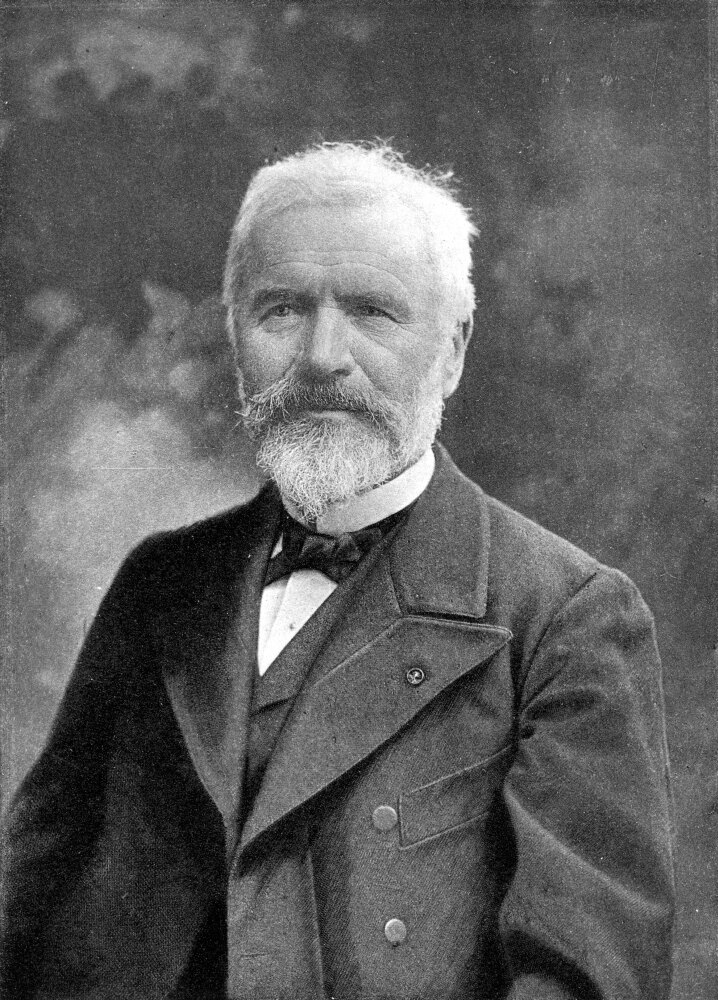
\includegraphics[width=5cm]{images/camille_jordan.jpg}
    \caption*{\centering Camille \textsc{Jordan} (1838 - 1922)}
\end{marginfigure}
\textsl{On doit à Camille \textsc{Jordan} de nombreux résultats sur la réduction des endomorphismes qu'il découvre notamment à travers l'étude des groupes. Dépassant la notion des groupes de permutations pour en atteindre une plus abstraite, il s'intéresse à la classification des groupes finis à travers leurs représentations linéaires, autrement dit les morphismes entre un groupe fini $G$ et le groupe linéaire $\Gl (E)$ d'un espace vectoriel $E$. Il va même jusqu'à donner le description des classes de similitudes à l'aide des formes dites de \textsc{Jordan}. \\
Le problème fondamental de la réduction est bien celui de caractériser les classes de similitude de l'algèbre $\Endo(E)$ où $E$ est un $\K$-espace vectoriel de dimension finie ou, ce qui revient au même, les classes de similitudes de l'agèbre $\M_n(\K)$. La recherche d'une matrice la plus simple possible pour représenter un endomorphisme donné vise de multiples buts: calculer les puissances successives de cet endomorphisme, son commutant, résoudre des systèmes différentiels linéaires... Une idée naturelle pour essayer de \say{ réduire } l'étude d'un endomorphisme $u$ donné à des choses plus simples consiste à essayer de décomposer l'espace vectoriel $E$ en une somme directe de sous-espaces non triviaux stables par $u$. Cela n'est évidemment pas toujours possible. Les sous-espaces stables les plus simples sont ceux sur lesquels $u$ coïncide avec une homothétie. On est ainsi naturellement amené à la notion de valeur propre. Si $\lambda$ est un scalaire, on s'intéresse donc au sous-espace $E_\lambda = \Ker(u - \lambda \Id_E)$ appelé sous-espace propre pour la valeur propre $\lambda$ lorsque celui-ci n'est pas nul. Le théorème de décomposition des noyaux nous assure que les différents sous-espaces propres d'un endomorphisme sont en somme directe. Le cas où la somme remplit tout l'espace $E$ mène à la notion d'endomorphisme diagonalisable: un tel endomorphisme peut être représenté par une matrice diagonale (il suffit de prendre une base formée de vecteurs propres). Pour les endomorphismes diagonalisables il est alors très facile de répondre à la question initiale de savoir quand ils sont semblables: il faut et suffit qu'ils aient les mêmes valeurs propres et que les espaces propres associés aient la même dimension. Il est aussi facile, en se ramenant à une matrice diagonale, de calculer les puissances d'un tel endomorphisme, son exponentielle (si on travaille sur un sous-corps de $\C$), son commutant...} \\

Soit $E$ un espace vectoriel de dimension finie. Un endomorphisme $u$ de $E$ est trigonalisable si et seulement s'il existe un drapeau total de $E$ stable par $u$. 

\begin{Large}
    Trigonalisation
\end{Large}

\textsl{La diagonalisation ne permet pas de caractériser toutes les classes de similitude de $\M_n(\K)$. Lorsque le corps de base est égal à $\C$, le polynôme caractéristique d'une matrice $A \in \M_n(\C)$ est toujours scindé et $A$ est alors trigonalisable. Le lemme des noyaux permet même dans ce cas de trigonaliser $A$ sous une forme diagonale par blocs avec pour chaque bloc diagonal une unique valeur propre. Cela conduit à la notion de sous-espace caractéristique et à la décomposition de \textsc{Jordan}-\textsc{Dunford}: dans le cas abstrait, tout endomorphisme $u$ d'un $\C$-espace vectoriel de dimension finie s'écrit de manière unique sous la forme $u = d + n$ où $d$ est diagonalisable, $n$ est nilpotent et commute avec $d$. (H.P. CPGE). Cette décomposition amène l'attention sur les classes de similitude des endomorphismes nilpotents. Avec un peu de travail il est alors possible d'obtenir le théorème de \textsc{Jordan} qui règle complètement la question de la détermination des classes de similitude sur un corps algébriquement clos. \\
Dans le cadre général, l'outil fondamental pour élucider les classes de similitude de $\M_n(\K)$ est la notion d'endomorphisme cyclique.
}

\newpage

\section{Matrice à diagonale dominante}
\begin{defi}{Matrice à diagonale dominante} 
    \\
    Soit $A \defeq (a_{i,j})_{1 \leqslant i, j \leqslant n} \in \M_n(\K)$. On dit que $A$ est 
    \begin{itemize}
        \item à \emph{diagonale dominante} si
        $$\forall i \in \llbracket 1, n \rrbracket,\ |a_{i,i}| \geqslant \sum_{k \not = i} |a_{i,k}|,$$
        \item à \emph{diagonale fortement dominante} si de plus l'inégalité est stricte pour une valeur de $i$ au moins,
        \item à \emph{diagonale strictement dominante} si l'inégalité est stricte pour tout $i$. 
    \end{itemize}
\end{defi}

\begin{lemme} \label{lemme_hadamard}
    Toute matrice à diagonale strictement dominante (\textsc{dsd}) est inversible.
\end{lemme}

\marginnote[2cm]{
    \begin{methode}
    Penser à poser 
        $$\left |x_{i_0} \right | \defeq \max_{1 \leqslant i \leqslant n} |x_i|.$$
    \end{methode}
}

\begin{preuve}
    Soit $X \defeq \Trsp{(x_1 \cdots x_n)} \in \Ker(A)$. \\
    On pose $\displaystyle \left |x_{i_0} \right| \defeq \max_{1 \leqslant i \leqslant n} |x_i|$. La ligne $i_0$ de la relation $AX = 0$ donne
    $$\sum_{j=1}^n a_{i_0,j}x_j = 0$$
    soit
    $$-a_{i_0, i_0} x_{i_0} = \sum_{j \not = i_0} a_{i_0,j} x_j$$
    d'où, d'après l'inégalité triangulaire,
    $$|a_{i_0, i_0}| |x_{i_0}| \leqslant \sum_{j \not = i_0} |a_{i_0,j}| |x_j| \leqslant |x_{i_0}| \sum_{j \not = i_0} |a_{i_0, j}|.$$
    Comme $|a_{i_0, i_0}| > \sum\limits_{j \not = i_0} |a_{i_0, j}|$ par définition de $A$, on en déduit que
    $|x_{i_0}| = 0$, autrement dit $X = 0$. Le noyau de $A$ est donc réduit au vecteur i.e. la matrice $A$ est inversible. \\
    Pour une autre démonstration voir \cite{matrices} page 51. 
\end{preuve}

\subsection{Localisation des valeurs propres}

À défaut de ne pas toujours pouvoir calculer exactement les valeurs propres d'une matrice, nous pouvons essayer de les localiser en restreignant autant que faire se peut le \say{ domaine } dans lequel elles se trouvent.

\begin{theo}{Localisation des valeurs propres} \labthm{localisation_des_vap}
    Soit $A \in \M_n(\K)$. Alors, $$\Sp(A) \subset \bigcup\limits_{i=1}^{n} \overline{\mathscr{B}} \Bigg( a_{i,i}, \sum\limits_{k \not = i} |a_{i,k}| \Bigg).$$
\end{theo}

\begin{preuve}
    Soit $\lambda \in \Sp(A)$. La matrice $A - \lambda \I_n$ n'est pas inversible \note 
    \marginnote[0cm]{\note Par définition $\det(A-\lambda \I_n) = \chi_A(\lambda) = 0$.}
    donc n'est pas à \textsc{dsd} i.e. pour tout $i \in \llbracket 1, n \rrbracket$,
    $$|a_{i,i} - \lambda| \leqslant \sum_{k \not= i} |a_{i,k}|.$$
    Le spectre de la matrice $A$ est donc inclus dans la réunion des disques de centre $a_{i,i}$ et de rayon $\sum\limits_{k \not=i} a_{i,k}$.
\end{preuve} 

\begin{defi}{Disques de \textsc{Gerschgorin}}
    Ces disques sont nommés les disques de \textsc{Gerschgorin} \note (cf. thème \textit{Localisation des valeurs propres}, Ch. 11 \cite{acamanes})
\end{defi}

\marginnote[-2cm]{
    \note Prenons un exemple en considèrant la matrice à coefficients complexes
    $$
    \begin{pmatrix}
        \textcolor{red}{\i4} & 0 & 2 & \i3 \\
        1 & \textcolor{blue}{5+\i10} & 5 & -1 \\
        0 & 2 & \textcolor{ForestGreen}{1} & 0 \\
        1 & 2 & 0 & \textcolor{orange}{-8-\i2}
    \end{pmatrix}.
    $$
    Ci-dessous sont représentés ses disques de \textsc{Gerschgorin} et les croix correspondent à ses valeurs propres.
}

\begin{marginfigure}
    \centering
    % This file was created with tikzplotlib v0.10.1.
\begin{tikzpicture}

\definecolor{dimgray85}{RGB}{85,85,85}
\definecolor{gainsboro229}{RGB}{229,229,229}
\definecolor{green}{RGB}{0,128,0}
\definecolor{lightgray204}{RGB}{204,204,204}
\definecolor{orange}{RGB}{255,165,0}

\begin{axis}[
axis lines=middle,
inner axis line style={-latex},
grid=major,
width=6cm,
height=6cm,
xtick=\empty,
xmin=-15, xmax=15,
ytick=\empty,
ymin=-10, ymax=20,
]
\draw[draw=red,fill=red,opacity=0.5,very thin] (axis cs:0,4) circle (5);
\draw[draw=blue,fill=blue,opacity=0.5,very thin] (axis cs:5,10) circle (7);
\draw[draw=green,fill=green,opacity=0.5,very thin] (axis cs:1,0) circle (2);
\draw[draw=orange,fill=orange,opacity=0.5,very thin] (axis cs:-8,-2) circle (3);

\def\r{3}

%\addplot [semithick, red, mark=*, mark size=\r, mark options={solid}, only marks]
%table {%
%0 4
%};
%\addlegendentry{1\mi}
%\addplot [semithick, blue, mark=*, mark size=\r, mark options={solid}, only marks]
%table {%
%5 10
%};
%\addlegendentry{(5+10\mi)}
%\addplot [semithick, green, mark=*, mark size=\r, mark options={solid}, only marks]
%table {%
%1 0
%};
%\addlegendentry{(1)}
%\addplot [semithick, orange, mark=*, mark size=\r, mark options={solid}, only marks]
%table {%
%-8 -2
%};
%\addlegendentry{(-8-2j)}

\addplot [semithick, black, mark=x, mark size=\r, mark options={solid}, only marks, forget plot]
table {%
-8.06720901070025 -2.31297809243462
};
\addplot [semithick, black, mark=x, mark size=\r, mark options={solid}, only marks, forget plot]
table {%
5.36805383956579 9.13980083948909
};
\addplot [semithick, black, mark=x, mark size=\r, mark options={solid}, only marks, forget plot]
table {%
0.195375871819944 4.3072164295875
};
\addplot [semithick, black, mark=x, mark size=\r, mark options={solid}, only marks, forget plot]
table {%
0.503779299314509 0.865960823358021
};
\end{axis}

\end{tikzpicture}
\end{marginfigure}

\begin{corol}
    Soit $A \defeq (a_{i,j})_{1 \leqslant i, j \leqslant n} \in \M_n(\K)$. On note
    \begin{equation*}
        E &\defeq \bigcup\limits_{i=1}^{n} \overline{\mathscr{B}} \Bigg( a_{i,i}, \sum\limits_{k \not = i} |a_{i,k}| \Bigg) \quad
        E' &\defeq \bigcup\limits_{i=1}^{n} \overline{\mathscr{B}} \Bigg( a_{i,i}, \sum\limits_{j \not = i} |a_{j, i}| \Bigg).
    \end{equation*}
    Alors,
    $$\Sp(A) \subset E \cap E'.$$
\end{corol}

\begin{preuve}
    D'après le théorème \ref{localisation_des_vap}, 
    $$\Sp(A) \subset E \text{ et } \Sp \big( \Trsp{A} \big) \subset E'.$$
    Or $\Sp(A) = \Sp \big( \Trsp{A} \big)$ donc $\Sp(A) \subset E \cap E'$.
\end{preuve}    

Ce corollaire permet de restreindre davantage le domaine où se trouvent les valeurs propres d'une matrice. 

\begin{prop}{}
    Soit $A \in \M_n(\R)$ à \textsc{dsd} telle que $a_{i,i} > 0$ pour tout $i \in \llbracket 1, n \rrbracket$. Alors $\mathrm{det}(A) > 0$. 
\end{prop}

\begin{preuve}
        $\det(A) = \prod\limits_{\lambda \in \Sp(A)} \lambda$. Distinguer les vap complexes et réelles...
\end{preuve}


\section{Matrices stochastiques}
\marginnote[3cm]{
    $$
    \begin{pmatrix}
    1/2 & 1/2 & 0 \\
    3/4 & 1/8 & 1/8 \\
    0 & 1/3 & 2/3
    \end{pmatrix}
    $$
}

\begin{marginfigure}[5cm]
    \centering
    \resizebox{6.5cm}{6.5cm}{%
    \begin{tikzpicture}
        \node[state] (s1) {1};
        \node[state, below right of=s1] (s2) {2};
        \node[state, below left of=s1] (s3) {3};
    
        \draw (s1) edge[loop above] node {$1/2$} (s1);
        \draw (s1) edge[bend left] node {$1/2$} (s2);
        %\draw (s1) edge[bend right, above left] node {0} (s3);
    
        \draw (s2) edge[bend left, above right] node {$3/4$} (s1);
        \draw (s2) edge[loop right] node {$1/8$} (s2);
        \draw (s2) edge[bend right] node {$1/8$} (s3);
    
        %\draw (s3) edge[bend right] node {0} (s1);
        \draw (s3) edge[bend right] node {$1/3$} (s2);
        \draw (s3) edge[loop left] node {$2/3$} (s3);
    \end{tikzpicture}    
}

  %  \begin{tikzpicture}
  %      \node[state] (s1) {État 1};
  %      \node[state, below right of=s1] (s2) {État 2};
   %     \node[state, below left of=s1] (s3) {État 3};
 %  
 %       \draw (s1) edge[loop above] node {$p_{1,1}$} (s1);
%        \draw (s1) edge[bend left] node {$p_{1,2}$} (s2);
%        \draw (s1) edge[bend right, above left] node {$p_{1,3}$} (s3);
    
 %       \draw (s2) edge[bend left, above right] node {$p_{2,1}$} (s1);
%        \draw (s2) edge[loop right] node {$p_{2,2}$} (s2);
%        \draw (s2) edge[bend right] node {$p_{2,3}$} (s3);
    
%        \draw (s3) edge[bend right] node {$p_{3,1}$} (s1);
%        \draw (s3) edge[bend right] node {$p_{3,2}$} (s2);
%        \draw (s3) edge[loop left] node {$p_{3,3}$} (s3);
%    \end{tikzpicture}    
    \caption*{\centering Une chaîne de \textsc{Markov} et sa matrice de transition.}
\end{marginfigure}

Texte de \cite{oraux_x_ens_2} p. 59 \\
Les matrices stochastiques interviennent en probibilités. Si $X$ et $Y$ sont deux variables aléatoires à valeurs dans $E \defeq \llbracket 1, k \rrbracket$, alors la matrice $A \defeq (a_{i,j}) \in \M_k(\R)$ définie par $a_{i,j} = \P(Y = j | X = i)$ est stochastique, ce qui par définition signifie qu'on a $a_{i,j} \geqslant 0\ (1 \leqslant i, j \leqslant k)$ et $\sum\limits_{j=1}^k a_{i,j} = 1\ (1 \leqslant i \leqslant k)$. \\
L'évolution d'un système susceptible de prendre un nombre fini d'états notés $1, \dots, k$ est représentée mathématiquement par une suite $(X_n)_{n \geqslant 0}$ de variables aléatoires à valeurs dans $E$. C'est ce qu'on appelle un processus aléatoire (ou stochastique). Si $X_{n+1}$ s'obtient à partir de la valeur de $X_n$ et d'un tirage au sort effectué selon une loi ne dépendant que de cette valeur, on dit que le processus est une chaîne de \textsc{Markov}. Les exemples abondent: marches aléatoires, fortune d'un joueur, modélisation de l'alternance des voyelles et des consonnes dans un poème de \textsc{Pouchkine} (par \textsc{Markov} lui-même), ou prévision (en probabilité) des états  successifs d'un signal pour améliorer la compression en traitement du signal (\textsc{Shannon}) \\
Techniquement, on dit qu'une suite de variables aléatoires $(X_n)$ est une chaîne de \textsc{Markov} si \say{ la loi de l'état $n+1$ conditionnelle au passé de dépend que de l'état antérieur $n$ }, ce qui se traduit par
$$\P(X_{n+1}=j | X_0=i_0, \dots, X_n = i_n) = \P(X_{n+1} = j | X_n = i_n).$$
Si la matrice $(A) \defeq (a_{i,j}) \in \M_k(\R)$ définie par $a_{i,j} = \P(X_{n+1} = j | X_n = i)$ est indépendante de $n$, on dit que la chaîne de \textsc{Markov} est stationnaire. Si, dans ce dernier cas, on pose $Y_n \defeq \begin{pmatrix} \P(X_n = 1) \\ \vdots \\ \P(X_n = k) \end{pmatrix}$, pour tout $n \geqslant 0$, on obtient $Y_{n+1} = A Y_n$ et donc $Y_n = A^n Y_0$. \\
Le comportement (probabiliste) d'une chaîne de \textsc{Markov} stationnaire, et notamment son comportement asymptotique, est donc entièrement décrit par la donnée de la loi initiale $Y_0$ et des puissances de la matrice $A$. 

\begin{defi}
    Une matrice stochastique (matrice de transition d'une \nameref{chaîne_markov}) est une matrice $P \in \M_n([0, 1])$ telle que pour tout $i \in \llbracket 1, n \rrbracket, \sum\limits_{j=1}^{n} p_{i,j} = 1$. \\ Autrement dit, chaque ligne de $P$ est une vecteur de probabilité. \\
    On dit que $P$ est \emph{doublement stochastique} si $P$ et $\Trsp{P}$ sont stochastiques.
\end{defi}

\begin{exercice}
    \footnote{Exercice 5, TD 11} \\
    Soit $P$ une matrice stochastique.
    \begin{enumerate}
        \item Montrer que $1$ est valeur propre de $P$.
        \item Soit $v = \Trsp{(v_1 \cdots v_n)}$ un vecteur propre associé à la valeur propre $1$. En considérant $|v_{i_0}| = \max\limits_{1 \leqslant i \leqslant n} |v_i|$, montrer que le sous-espace propre associé à $E_1$ est de dimension $1$.
        \item Montrer que si $\lambda \in \C$ est une valeur propre de $P$, alors $| \lambda | \leqslant 1$.
        \item Soit $\lambda \in \C$ une valeur propre de $P$ telle que $|\lambda| = 1$ et $\title{x}$ un vecteur propre associé.
        \begin{enumerate}
            \item Montrer qu'il existe un vecteur propre associé à $\lambda$ tel que $\Ninf{x} = 1$. 
            \item Montrer qu'il existe $i_0 \in \llbracket 1, n \rrbracket$ tel que $\left| \sum\limits_{j=1}^n p_{i_0,j} x_j \right| = 1$.
            \item Soit $\theta$ l'argument principal de $\sum\limits_{j=1}^n p_{i_0,j} x_j$. Montrer que pour tout $j \in \llbracket 1, n \rrbracket, \Reel \left( \me^{-\mi \theta} x_j \right) = 1$.
            \item En déduire que $\lambda = 1$.
        \end{enumerate}
    \end{enumerate}
\end{exercice}

\begin{solution}
    L'objectif de l'exercice est de montrer que $\boxed{\Sp_{\C}(P) = \{1 \} }$.
    \begin{enumerate}
        \item 1 est valeur propre évidente de $P$ de vecteur propre associé $v = (1, \dots, 1)^\top$.
        \item Montrer que $\dim E_1 = 1$.
        \begin{itemize}
            \item Appliquer la même méthode que la démonstration du lemme d'\textsc{Hadamard}. \\
            Soit $X = \Trsp{(x_1, \dots, x_n)} \in E_1$. Montrons que $X \in \Vect(v)$. \\
            On montre que $|x_{i_0}| = \left| \sum\limits_{j=1}^{n} p_{i_0, j} x_j \right| = \sum\limits_{j=1}^{n} p_{i_0, j} |x_j|$ et on écrit $|x_{i_0}| = |x_{i_0}| \sum\limits_{j=1}^{n} p_{i_0, j}$. D'où, en faisant la différence, pour tout $j \in \llbracket 1, n \rrbracket,\ |x_{i_0}| = |x_j|$. De plus d'après la première relation, il y égalité dans l'inégalité triangulaire et donc les $v_j$ sont \emph{positivement liées}. Finalement, pour tout $j \in \llbracket1, n \rrbracket,\ v_j = v_{i_0}$ soit $\dim E_1 = 1$.
        \end{itemize}
        \item Montrer que si $\lambda \in \C$ est une valeur propre de $P$, alors $|\lambda| \leqslant 1$. \\
        Poser $X = (x_1, \dots, x_n)^\top$ un vecteur propre associé et appliquer encore une fois la même méthode; poser $\displaystyle |x_{i_0}|= \max_{1 \leqslant i \leqslant n} |x_i|$, écrire en module la ligne $i_0$ de l'égalité $\lambda X = P X$, diviser par $|x_{i_0}|$ (qui est non nul d'après la question précédente) puis majorer par $1$. \\
            
        Pour les curieux, lire \cite{matrices} page 59. 
        
        \begin{prop}
            Le \nameref{rayon_spectral} stochastique est égal à $1$.
        \end{prop}
    
        \item Les questions suivantes (à détailler éventuellement) consiste encore au même jeu avec la ligne $i_0$ et les propriétés de matrices stochastiques. 
    \end{enumerate}
\end{solution}


\section{Endomorphismes semi-simples}
\begin{prop}[Critère de diagonalisabilité dans un $\R$-ev]
    Soit $E$ un $\R$-espace vectoriel de dimension finie, soit $f \in \Endo(E)$. Alors $f$ est diagonalisable si et seulement si tout sous-espace vectoriel de $E$ admet un supplémentaire stable par $f$.
\end{prop}

\begin{demo}
    \source{à compléter}
    \begin{itemize}
        \item[$(\Leftarrow)$] Supposons $f$ diagonalisable. Soit $F$ un sous-espace vectoriel quelconque de $E$. Soit $(e_1, \dots, e_m)$ une base de $F$. Puisqu'on a supposé $f$ diagonalisable, il exsite une base $(v_1, \dots, v_n)$ de $E$ formée de vecteurs propres pour $f$. D'après le théorème de la base incomplète, on peut compléter la base $(e_1, \dots, e_m)$ de $F$ en une base $(e_1, \dots, e_m, e_{m+1}, \dots, e_n)$ de $E$, où on rajouté uniquement des vecteurs de notre base de vecteurs propres (c'est-à-dire $e_{m+1}, \dots, e_n$ ont été pris parmi les $v_i$). En effet, la famille $(e_1, \dots, e_m)$ est libre, et elle est contenue dans la famille génératrice $(e_1, \dots, e_m, v_1, \dots, v_n)$, donc il existe une famille $\mathcal{F}$ de vecteurs de $E$, telle que 
        $$(e_1, \dots, e_m) \subseteq \mathcal{F} \subseteq (e_1, \dots, e_m, v_1, \dots, v_n)$$
        et $\mathcal{F}$ à la fois libre et génératrice. \\
        \textcolor{red}{il manque une explication supplémentaire} \\
        On prend alors $G \defeq \Vect(e_{m+1}, \dots, e_n)$. C'est un supplémentaire de $F$ dans $E$, et il est stable par $f$ car $e_{m+1}, \dots, e_n$ sont des vecteurs propres de $f$.
        \item[$(\Rightarrow)$] Réciproquement, supposons que tout sous-espace vectoriel de $E$ admet un supplémentaire stable par $f$. Considérons
        $$F \defeq \smashoperator{\bigoplus_{\lambda \in \Sp f}} \Ker(f - \lambda \Id)$$
        le sous-espace vectoriel de $E$ formé de la somme directe des sous-espaces propres de $f$. Si $f$ n'était pas diagonalisable, $F$ serait strictement inclus dans $E$. Soit $H$ un hyperplan de $E$ contenant $F$. Alors par hypothèse $H$ admet un supplémentaire stable par $f$. Ce supplémentaire est une droite, engendrée par un vecteur propre de $f$. Mais c'est une contradiction car tous les vecteurs propres de $f$ sont dans $H$. Ainsi, $f$ est diagonalisable. 
    \end{itemize}
\end{demo}

Nous allons maintenant définir la notion d'endomorphisme semi-simple en relâchant un peu la
condition de l'exercice ci-dessus : nous allons seulement demander aux sous-espaces stables de posséder
un supplémentaire stable.

\begin{defi}[Endomorphisme semi-simple]
    Un endomorphisme $u$ est dit \emph{semi-simple} si tout sous-espace stable par $u$ admet un supplémentaire stable par $u$.
\end{defi}

\begin{prop}[Critère de diagonalisabilité sur un $\C$-ev]
    Soient $E$ un $\C$-espace vectoriel de dimension finie non nulle et $u \in \Endo(E)$. Alors l'endomorphisme $u$ est semi-simple si et seulement s'il est diagonalisable.
\end{prop}

\begin{demo}
    \begin{itemize}
        \item[$(\Leftarrow)$] On suppose que l'endomorphisme $u$ est diagonalisable. \\
        Son polynôme caractéristique est scindé ce que l'on voit en mettant $u$ sous forme diagonale, et par invariance de $\chi$ par changement de base. \\
        Soit $F$ un sous-espace de $E$. Soit $(e_1, \dots, e_n)$ une base de vecteurs propres de $u$ et $(f_1, \dots, f_p)$ une base de $F$. Par le théorème de la base incomplète, on peut compléter la famille libre $(f_1, \dots, f_p)$ en une base de $E$ en rajoutant $n-p$ vecteurs parmi la base $(e_1, \dots, e_n)$, quitte à réindexer, on peut supposer que c'est $(e_{p+1}, \dots, e_n)$, ces vecteurs engendrent alors un sous-espace stable supplémentaire de $F$.
        \item[$(\Rightarrow)$] On construit une base de vecteurs propres de la manière suivante: prenons un hyperplan $H$ quelconque, il existe une droite stable supplémentaire, donc dirigée par un vecteur propre $e_1$. Si on a construit une famille libre de vecteurs propres $(e_1, \dots, e_k)$, on prend un hyperplan contenant $\Vect(e_1, \dots, e_k)$, et on trouve une droite stable $\Vect(e_{k+1})$ supplémentaire à $H$. On conclut par récurrence.
    \end{itemize}
\end{demo}

Notes de la correction vue en cours.
\begin{demo}
    \begin{itemize}
        \item[$(\Leftarrow)$] Soit $F$ un sev de $E$ stable par $f$.
        Posons $g \defeq f_{\vert F}$ qui est diagonalisable car $f$ l'est par hypothèse. \\
        Soit $\mathscr{B}_F$ une base de $F$ formée de vep de $g$. \\
        Soit $\mathscr{B}'$ une base de $E$ formée de vep de $f$ (qui existe car $f$ est diagonalisable). \\
        On complète $\mathscr{B}_F$ est une base $\mathscr{B}$ de E en prenant des vep $(\varepsilon_1, \cdots, \varepsilon_r)$ de $\mathscr{B}'$. On note $(\lambda_1, \dots, \lambda_r)$ les valeurs propres associées. \\
        On pose $G = \mathrm{Vect}(\varepsilon_1, \dots, \varepsilon_r)$. De cette manière, $F$ et $G$ sont supplémentaires. Montrons que $G$ est stable par $f$. \\
        Soit $x = \sum\limits_{i=1}^{r} \mu_i \varepsilon_i \in G$. Donc $f(x) = \sum\limits_{i=1}^{r} \mu_i f(\varepsilon_i) =  \sum\limits_{i=1}^{r} \mu_i \lambda_i \varepsilon_i \in G$ et $G$ est stable par $f$.
    
        \item[$(\Rightarrow)$] Montrons que $f$ est diagonalisable. On va montrer que $E = \smashoperator{\bigoplus\limits_{\lambda \in \Sp(f)}} E_\lambda (f)$.
        
        \begin{enumerate}
            \item \underline{Somme directe:} \\
            On pose $F = \smashoperator{\bigoplus\limits_{\lambda \in \Sp(f)}} E_\lambda (f)$ et $\Sp(f) = (\lambda_1, \dots, \lambda_r)$. \\
            Soit $x = \sum\limits_{i=1}^{r} x_i \in F$ où $x_i \in E_{\lambda_i}(f)$. Alors $f(x) = \sum\limits_{i=1}^{r} \underbrace{\lambda_i x_i}_{\mathclap{\in E_{\lambda_i}(f)}} \in F$. Donc $F$ est stable par $f$.
            \item Montrons que $F = E$. \\
            Par hypothèse, $F$ admet un supplémentaire $G$ dans $\C^n$, stable par $f$. Montrons que $G = \{0\}$ en raisonnant par l'absurde. \\
            On pose $g = f_{\vert F}$. D'après le théorème de \textsc{D'Alembert-Gauss} sur $\C$, $g$ admet au moins une valeur propre $\mu \in \C$ de vep associé $x_\mu$. On montre que $x_\mu \in F \cap G$. Or $F$ et $G$ sont supplémentaires donc $x_\mu = 0_E$: contradiction. D'où le résultat. 
        \end{enumerate}
        \item Considérer $R_\theta$. \textcolor{green}{à revoir}
    \end{itemize}
\end{demo}

\begin{exercice}
    Décrire un contre-exemple à la réciproque dans $\R$, en dimension 2.
\end{exercice}  

\section{Autour du commutant}
\marginnote[0cm]{Exercice 12 TD 11}

\begin{defi}
    Soient $A \in \M_n(\R)$ et $C(A) \defeq \{ M \in \M_n(\R);\ MA = AM \}$.
\end{defi}

\emph{Toutes les questions ne sont pas abordées}

\begin{enumerate}
    \item \emph{Montrer que C(A) est un sous-espace vectoriel de $\M_n(\R)$.} \\
    Au lieu de redémontrer les propriétés d'un sev, on peut voir $C(A)$ comme le \textbf{noyau de l'application linéaire} $M \mapsto MA - AM$ ce qui donne directement le résultat. 
    \item \emph{Montrer que si $M \in C(A)$ et $M$ est inversible, alors $M^{-1} \in C(A)$.} \\
    On veut montrer que $M^{-1} A = A M^{-1}$ i.e. $A = M A M^{-1}$ ce qui est vrai car $M A = A M$.
    \item \emph{Soit $D$ une matrice diagonale dont les coefficients diagonaux notés $(d_i)_{i \in \llbracket 1, n \rrbracket}$ sont deux à deux distincts. Déterminer $C(D)$ et montrer que $\mathscr{B} = (I_n, D, \dots, D^{n-1})$ est une base de $C(D)$.}
    \begin{itemize}
        \item $C(D) = \mathscr{D}_n$ (l'ensemble des matrices diagonales de taille $n$) \textcolor{red}{(ne pas oublier de montrer la double inclusion)}.
        \item Comme $| \mathscr{B} | = \dim C(D)$, il suffit de montrer la liberté de $\mathscr{B}$. \\
        Soit $(\lambda_0, \dots, \lambda_{n-1}) \in \R^n$ tel que $\sum\limits_{k=0}^{n-1} \lambda_k D^k = 0_n$. \\
        \textcolor{green}{Revoir le caractère générateur avec les polynômes d'interpolation.}
        \begin{itemize}
            \item Pour tout $i \in \llbracket 1, n \rrbracket$, $\sum\limits_{k=0}^{n-1} \lambda_k d_i = 0_n \quad (*)$. Donc le polynôme $P = \sum\limits_{k=0}^{n-1} \lambda_k X^k$ qui est de dégré $n-1$ et prossède $n$ racines distinctes et est donc le polynôme nul. On en déduit que les $\lambda_i$ sont tous nuls. La famille $\mathscr{B}$ est bien libre et forme une base de $C(D)$.
            \item Les relations $(*)$ forment un système de \textsc{Vandermonde} de $n$ équations à $n$ inconnues. Comme les coefficients $d_i$ sont deux à deux distincts, le système est inversible et son unique solution est le vecteur colonne nul.
        \end{itemize}
    \end{itemize}
    \item On se limite au cas $n = 2$. 
    \begin{enumerate}
        \item Déterminer les matrices $A$ telles que $\dim C(A) = 4$. \\
        $C(A) = \M_2(\R)$ car $C(A) \subset \M_2(\R)$ et il y égalité des dimensions. \\
        \textbf{Évaluer les commutant en les matrices de la base canoniques de $\M_2(\R)$}: on trouve que A est scalaire. \\
        \textcolor{red}{Ne pas oublier de montrer la réciproque}. 
        \item Montrer que $\dim C(A) \geqslant 2$. \\
        Si $A$ est scalaire, cf. question précédente. \\
        Sinon montrer que la famille $\{ \I_2, A \} \subset C(A)$ est libre. 
        \item Enoncé... \\
    \end{enumerate}
\end{enumerate}

\section{Matrice circulante} %%%%%%%%%%%%%%%%%%%%%%%%%%%%%%%%%%% Déterm  
\begin{tcolorbox}
Une \href{https://fr.wikipedia.org/wiki/Matrice_circulante}{\emph{matrice circulante}} est une matrice carrée dans laquelle on passe d'une ligne à la suivante par permutation circulaire des coefficients:
$$
\mathrm{C}(c_0, \dots, c_{n-1})=
\begin{pmatrix}
c_0 & c_1 & c_2 & \cdots & c_{n-1} \\
c_{n-1} & c_0 & c_1 & \cdots & c_{n-2} \\
c_{n-2} & c_{n-1} & c_0 & \cdots & c_{n-3} \\
\vdots & \vdots & \vdots & \ddots & \vdots \\
c_1 & c_2 & c_3 & \cdots & c_0
\end{pmatrix}.
$$
\end{tcolorbox}

\begin{remarque}
    Une matrice circulante est un cas particulier de \href{https://fr.wikipedia.org/wiki/Matrice_de_Toeplitz}{matrice de \textsc{Toeplitz}}.
\end{remarque}

\begin{prop}
On pose $\omega = \me^{\mi \frac{2 \pi}{n}}$.
    $$\Sp(\mathrm{C}(c_0, \dots, c_{n-1})) = \left \{ \sum_{j=0}^{n-1} c_j \omega^j,\ k \in \llbracket 1, n-1 \rrbracket \right \}.$$
\end{prop}

\begin{preuve}
    Pour alléger les notations, on pose $\mathrm{C} := \mathrm{C}(c_0, \dots, c_{n-1})$. \\
    On pose 
    $$
    \mathrm{J} = 
    \begin{pmatrix}
    0 & 1 & 0 & \cdots & 0 \\
    \vdots  &   & \ddots & \\
    0 & & & & 1 \\
    1 & 0 & \cdots & \cdots & 0
    \end{pmatrix}
    $$
    
    (faire une remarque sur la structure de la matrice J et que J$^n = \I_n$) 
    
    $$\mathrm{C} = \sum_{k=0}^{n-1} c_k \mathrm{J}^k = \mathrm{P}_{\mathrm{C}}(\mathrm{J}).$$
    
    En développant par rapport à la première colonne, 
    \begin{align*}
        \chi_{\mathrm{J}}(X) &= 
        \begin{vmatrix}
            X & -1 & 0 & \cdots & 0 \\
            \vdots  &   & \ddots & \\
            0 & & & & -1 \\
            -1 & 0 & \cdots & \cdots & X
        \end{vmatrix} \\
        &= X \times X^{n-1} + (-1) \times (-1)^{n+1} \times (-1)^{n-1} \\
        \chi_{\mathrm{J}}(X) &= X^n-1. 
    \end{align*}
    Le polynôme caractéristique de $\mathrm{J}$ est scindé à racines simples sur $\C$ donc $\mathrm{J}$ est diagonalisable et en posant $\omega = \me^{\mi \frac{2 \pi}{n}}$, 
    $$\Sp(\mathrm{J}) = \mathbb{U}_n = \left \{ \omega^k,\ k \in \llbracket 0, n-1 \rrbracket \right \}.$$
    Ainsi, $\mathrm{J}$ est semblable à la matrice 
    $$
    \begin{pmatrix}
    1 & & & & \\
    & \omega & & & \\
    & & \omega^2 & & \\
    & & & \ddots & \\
    & & & & \omega^{n-1} \\
    \end{pmatrix}
    $$
    et donc comme $\mathrm{C} = \mathrm{P}_{\mathrm{C}}(\mathrm{J})$, la matrice $\mathrm{C}$ est semblable à  la matrice
    $$
    \begin{pmatrix}
    \mathrm{P}(1) & & & & \\
    & \mathrm{P}(\omega) & & & \\
    & & \mathrm{P}(\omega^2) & & \\
    & & & \ddots & \\
    & & & & \mathrm{P}(\omega^{n-1}) \\
    \end{pmatrix}.
    $$
    Ainsi, $\Sp(\mathrm{C}) = \left \{ \mathrm{P}(\omega^k),\ k \in \llbracket 0, n-1 \rrbracket \right \}$.
\end{preuve}

\begin{corol}
    $$\det(\mathrm{C}(c_0, \dots, c_{n-1})) = \prod_{j=0}^{n-1} \left( \sum_{k=0}^{n-1} c_k \exp \left( \mi \frac{2kj \pi}{n} \right) \right).$$
\end{corol}

\begin{preuve}
    Le déterminant d'une matrice est égal au produit de ses valeurs propres.
\end{preuve}


\section{Que dire si \texorpdfstring{$M^2$}{M^2} est diagonalisable ?}
\begin{prop}{Critère de diagonalisabilité}
    Soient $n \in \Ne$ et $M \in \M_n(\C)$. On suppose que la matrice $M^2$ est diagonalisable. Alors $M$ est diagonalisable si et seulement si $\Ker M = \Ker M^2$.
\end{prop}

\begin{preuve}
    \begin{itemize}
        \item[$(\Rightarrow)$] 
        %$(\Rightarrow)$ On suppose que $M$ est diagonalisable (et donc $f$ aussi). Notons $(\lambda_1, \dots, \lambda_n) \in \C^n$ les valeurs propres de $f$. Il existe une base $\mathscr{B}$ telle que $\mathrm{Mat}_{\mathscr{B}}(f) = \mathrm{Diag}(\lambda_1, \dots, \lambda_n)$. Donc $\mathrm{Mat}_{\mathscr{B}}(f^2) = \mathrm{Diag}(\lambda_1^2, \dots, \lambda_n^2)$. \\
        Supposons que la matrice $M$ est diagonalisable. Montrons que $\Ker M^2 \subset \Ker M$ (l'autre inclusion est toujours vraie) \note . \\
        \marginnote[0cm]{\note 
            Soit $X \in \Ker M$. Alors,
            $$MX = 0$$
            d'où 
            $$M (M X) = M \times 0 = 0$$
            et 
            $$X \in \Ker M^2.$$
        }
        Voyons deux approches.
        \begin{itemize}
            \item Nous allons montrer \ptnclegras{l'égalité des dimensions} de ces deux espaces. \\
            Soient $u$ l'endomorphismes canoniquement associé à $M$ et $\mathscr{B}$ une base de diagonalisation de $u$. \ptnclegras{Le rang d'une matrice diagonale étant le nombre de coefficients diagonaux non nuls}, $\Rg \Mat_\mathscr{B}(u^2) = \Rg  \Mat_\mathscr{B}(u)$ donc $\Rg u^2 = \Rg u$ \note.
            \marginnote[0cm]{\note Le rang est un invariant de similitude.}
            Par le \ptnclegras{théorème du rang}, il s'ensuit que $\dim \Ker u^2 = \dim \Ker u$.
            \item Soit $X \in \Ker M^2$ i.e. $M^2 X = 0\ (\star)$. Montrons que $MX = 0$. L'idée est de \ptnclegras{faire apparaître un produit scalaire} sur l'ensemble des vecteurs colonnes d'une matrice i.e. une produit de la forme $N^\top N$. \\
            Comme $M^2$ est diagonalisable, il existe $P$ inversible et $D$ diagonale telles que $M^2 = PDP^{-1}$. En remplaçant $M^2$ par cette expression dans $(\star)$ puis en multipliant à gauche successivement par $P^{-1}$,  $(P^{-1})^\top$ et $X^\top$ on trouve $X^\top (P^{-1})^\top D^2 P^{-1} X = 0$ soit 
            $$(D P^{-1} X)^\top (D P^{-1} X) = 0.$$
            Comme $(C, C') \mapsto C^\top \times C'$ définit un produit scalaire sur l'espace des vecteurs colonnes, on a $D P^{-1} X = 0$ car il est orthogonal à lui-même et donc, en multipliant à gauche par $P$, nous obtenons bien $MX = 0$. 
        \end{itemize}
        \item[$(\Leftarrow)$] Supposons que $\Ker M = \Ker M^2$. Voyons encore deux approches.
        \begin{itemize}
            \item \cite{reduc_des_endo} p. 100 \note 
            \marginnote[0cm]{\note La clé de cette démonstration est l'équivalence
                \begin{center}
                    $M$ diagonalisable $\Leftrightarrow$ $\exists P \in \mathrm{Ann}(M)$ \textsc{sars}.
                \end{center}
            }
            \\
            Comme $M^2$ est diagonalisable, il existe $Q$ scindé à racines simples vérifiant $Q(0) \not= 0$ tel que $X Q(X)$ annule $M^2$, c'est-à-dire $M^2 Q(M^2) = 0$. \\
            Alors, pour tout $X \in E$, $Q(M^2)X \in \Ker M^2$; or $\Ker M^2 = \Ker M$ par hypothèse donc $Q(M^2)X \in \Ker M$ soit $M Q(M^2)X = 0$. \\
            Ainsi, $XQ(X^2)$ est un polynôme annulateur de $M$. Il suffit de remarquer que ce polynôme est scindé à racines simples (car les racines complexes de $Q$ sont deux à deux distinctes et non nulles) pour conclure avec le critère algébrique de diagonalisabilité que $M$ est diagonalisable.
            \item 
            Une démonstration alternative consiste à montrer que, pour tout $\lambda \in \Ce$ de racines carrées distinctes $\mu$ et $\mu'$, le sous-espace propre $u^2$ associé à $\lambda$ se décompose avec les sous-espaces propres $u$:
            $$\Ker(\lambda \Id_E - u^2) = \Ker(\mu \Id_E - u) \oplus \Ker(\mu' \Id_E - u).$$
            La condition porte alors que le sous-espace propre de $u^2$ associé à $0$, c'est-à-dire $\Ker(u^2)$.
            \underline{Notes de cours à traiter} \\
            Raisonnons par analyse-synthèse: soit $\lambda$ une valeur propre non nulle de $f^2$. Notons $\mu$ une racine carrée complexe de $\lambda$. Montrons que $E_{\lambda}(f^2) = E_{\mu}(f) \oplus E_{-\mu}(f)$. \\
            On pose $y = \frac{x}{2} + \frac{f(x)}{2 \mu}$ et $z = \frac{x}{2} - \frac{f(x)}{2 \mu}$. \\
            Comme $f^2$ est diagonalisable, $E$ est la somme directe des sous-espaces propres de $f^2$. On décompose chacun de ces sep comme ci-dessus et on en déduit que $E$ est la somme directe des sep de $f$ i.e. $f$ est diagonalisable. \\

        \end{itemize}
    \end{itemize}
\end{preuve}


\section{Raciné carrée d'une matrice}
\url{https://share.miple.co/content/CtwFAB5leFp4M}

\begin{box_titre}{DS6}
    On note $\mathrm{Rac}(A) = \{ R \in \M_n(\R),\ R^2 = A \}$. \\
    $\blacktriangleright$ Soit $A \in \M_n(\R)$. $\mathrm{Rac}(A)$ est une partie fermée de $\M_n(\R)$. \\
    $\blacktriangleright$ $\mathrm{Rac}(\I_n)$ n'est pas une partie bornée de $\M_n(\R)$ pour $n \geqslant 3$. 
\end{box_titre}

\begin{prop}{}
    Pour tout $A \in \mathscr{S}_n^+(\R)$, il existe une unique matrice $B \in \mathscr{S}_n^+(\R)$ telle que $A = B^2$. 
\end{prop}
\textcolor{red}{retrouver la source}
\begin{preuve}
    \underline{Existence:} comme la matrice $A$ est symétrique et positive, d'après le théorème spectral, il existe $\lambda_1, \dots, \lambda_r$ des réels positifs et $P \in \mathcal{O}_n(\R)$ tels que $A = \Inv{P} \Diag(\lambda_1, \dots, \lambda_r) P$. \\
    On pose $B = \Inv{P} \Diag(\sqrt{\lambda_1}, \dots, \sqrt{\lambda_r}) P$. \\
    La matrice $B$ vérifie $B^2 = A$, elle est bien symétrique car la matrice $P$ est orthogonale et $B$ est positive puisque symétrique à valeurs propres positives. \\
    \underline{Unicité:} supposons donné une matrice $C$ comme second candidat. \\
    Considérons $Q$ un polynôme vérifiant, pour $1 \leqslant i \leqslant r, Q(\lambda_i) = \sqrt{\lambda_i}$. Ainsi, 
    $$Q(A) = \Inv{P} Q\left(\Diag(\lambda_1, \dots, \lambda_r)\right) P = \Inv{P} \Diag(\sqrt{\lambda_1}, \dots, \sqrt{\lambda_r}) P = B.$$
    Par ailleurs, comme $C^2 = A$ alors $C$ et $A$ commutent. Par conséquent, $C$ commute avec tout polynôme en $A$ et commute donc avec $B$. \\
    Les matrices $B$ et $C$ étant diagonalisables (car symétriques) et commutant, elles sont codiagonalisables. \\
    Ainsi, il existe $R \in \Gl_n(\R)$, $D_1, D_2 \in \mathscr{D}_n(\R)$ telles que $\Inv{R}BR = D_1$ et $\Inv{R}CR = D_2$. \\
    Or $D_1^2 = \Inv{R} B^2 R = \Inv{R} A R = \Inv{R} C^2 R = D_2^2$. Les matrices $D_1$ et $D_2$ étant diagonales à coefficients positifs, on en déduit que $D_1 = D_2$. Ainsi, $B = C$.
\end{preuve}

\begin{exercice}
    \underline{Exercice 11, TD 11:}\\
    Soit $A = 
    \begin{pmatrix}
        -1 & 2 & 3 \\
        0 & - 1 & 4 \\
        0 & 0 & 1
    \end{pmatrix}. 
    $ Montrer que $A$ n'a pas de racine dans $\M_3(\R)$. 
\end{exercice}


\section{Réduction d'une matrice creuse}
\begin{tcolorbox}
    Soit $n \geqslant 2$. On pose:
    $$
    A = 
        \begin{pmatrix}
              &        &   & c \\
              &  (0)   &   & \vdots \\
              &        &   & c \\
            b & \cdots & b & a
        \end{pmatrix}
        \in \M_n(\R).
    $$
    Étudier la possibilité de diagonaliser $A$ sur $\R$.
\end{tcolorbox}

\underline{Remarques:}\\
$\blacktriangleright$ Si $b = c$ alors $A$ est symétrique réelle donc diagonalisable. \\
$\blacktriangleright$ $A$ est au plus de rang 2. Donc par le \textbf{théorème du rang}, 0 est une valeur propre de $A$ de multiplicité au moins $n-2$.

\section{Vecteurs propres de \texorpdfstring{$\Trsp{\com(A)}$}{la transposée de la comatrice}}
\begin{exercice}
    Soit $A \in \M_n(\K)$ et $B = \Trsp{\com(A)}$. Montrer que les vecteurs propres de $A$ sont des vecteurs propres de $B$. 
\end{exercice}

$$\boxed{A \times\ \com(\Trsp{A}) = \com(\Trsp{A}) \times A = \det(A) \I_n}$$

\begin{elem_sol}
    Soit $\lambda \in \Sp(A)$ et $X$ un vecteur propre associé. Alors $\lambda (BX) = \det(A) X$. 
        
    \begin{itemize}
        \item $\lambda \not = 0$: $BX = \frac{\det(A)}{\lambda}X$. 
        \item $\lambda = 0$: alors $\det(A) = 0$ et $\Rg(A) \leqslant n-1$. 
        \begin{itemize}
            \item $\Rg(A) \leqslant n-2$: supposer par l'absurde qu'il existe un déterminant mineur de $A$ non nul. 
            \item $\Rg(A) = n-1$: $X \in \Ker(A)$ qui est une droite vectorielle. 
            $$\boxed{A \text{ et } B \text{ commutent donc } \Ker(A) \text{ est stable par } B}$$
        \end{itemize}
    \end{itemize}
\end{elem_sol}


\section{Éléments propres de \texorpdfstring{$MN$}{MN}, de \texorpdfstring{$NM$}{NM}}
\begin{prop}{}
    Soient $M$ et $N$ dans $\M_n(\K)$.
    \begin{itemize}
        \item $$0 \in \Sp(MN) \Longleftrightarrow 0 \in \Sp(NM)$$
        \item Soit $\lambda \in \Ke$,
        $$\dim E_\lambda(MN) = \dim E_\lambda(NM)$$
    \end{itemize}
\end{prop}

Soit $M, N \in \M_n(\K)$. 
\begin{enumerate}
    \item ...
    \item \emph{Soit $\lambda \in \Ke$, montrer que $\dim(E_\lambda (MN)) = \dim(E_\lambda (NM))$.} \\
    On remarque que si $X \in E_\lambda (MN)$ alors $NX \in E_\lambda (NM)$. On pose alors:
    \begin{alignat*}{2}
        \varphi\ :\ E_\lambda (MN)\ &\longrightarrow\ E_\lambda (NM)\\
        X\ &\longmapsto\ NX
    \end{alignat*}
    On montre que $\varphi$ est injective et on en déduit que $\dim(E_\lambda (MN)) \leqslant \dim(E_\lambda (NM))$. Par symétrie des rôles de $M$ et de $N$, on montre l'inégalité dans le sens inverse et on en déduit l'égalité.
    \item ...
    \item ...
\end{enumerate}

\begin{defi}{Partie dense}
    \marginnote[0cm]{\url{https://www.bibmath.net/dico/index.php?action=affiche&quoi=./d/dense.html}}
    Soit $E$ un espace vectoriel normé et $D$ une partie de $E$. On dit que $D$ est \emph{dense} dans $E$ si l'une des conditions équivalentes suivantes est vérifiée:
    \begin{itemize}
        \item pour tout $x \in E$, il existe une suite $(y_n)$ d'éléments de $D$ qui converge vers $x$.
        \item pour tout $x \in E$, pour tout $\varepsilon > 0$, il existe $y \in D$ tel que $\norme{y - x} \leqslant \varepsilon$.
        \item l'adhérence $\overline{D}$ de $D$ est égale à $E$.
    \end{itemize}
\end{defi}

\subsection{Densité de \texorpdfstring{$\Gl_n(\C)$}{GL_n(C)} dans \texorpdfstring{$\M_n(\C)$}{M_n(C)}}

\begin{theo}{}
    L'ensemble des matrices inversibles de $\M_n(\C)$ est dense dans $\M_n(\C)$.
\end{theo}

\begin{marginfigure}[2cm]
    \centering
    \begin{tikzpicture}[scale=1.3]
  \definecolor{mylightred}{RGB}{255,210,210}
  \definecolor{myred}{RGB}{200,100,100}
  \definecolor{mylightred2}{RGB}{255,232,232}
      \def\ang{150}
      \def\R{1}
      \coordinate (O)  at (0, 0);
      \coordinate (L1) at (30:1);
      \coordinate (L2) at (-1, -1.5);
      \coordinate (L3) at (1.5, -1);
      \coordinate (L4) at (1.2, 1);
      \coordinate (L5) at (-1.1, 1.1);
     
      \draw[-latex] (0, -1.6) -- (0, 1.6);
      \draw[-latex] (-2, 0) -- (2, 0);
      \fill[radius=0.8pt,black] (O) circle;
      \draw[mylightred, fill, opacity=0.5] (O) circle (\R);
      \draw[myred, dashed] (O) circle (\R);
      \fill[radius=0.8pt,blue]
        (L1) circle node[above right=-1pt] {$\lambda_1$}
        (L2) circle node[above left =-1pt] {$\lambda_2$}
        (L3) circle node[above right=-1pt] {$\lambda_3$}
        (L5) circle node[below left =-1pt] {$\lambda_4$};
      \draw (0.6, -0.04) -- (0.6, 0.04)  node[above] {$t$};
      \draw[latex-latex, myred] (O) -- (\ang:\R) node[midway] {\contour{mylightred2}{$r$}};
\end{tikzpicture}
\end{marginfigure}

\begin{preuve}
    Soit $A \in \M_n(\K)$. Son polynôme caractéristique $\chi_A$ est de degré $n$ et admet donc au plus $n$ racines. \\
    Notons $r \defeq \min \big\{ |\lambda|, \lambda \in \Sp(A) \setminus \{0\} \big\}$. \\
    Ainsi,
    $$\forall t \in ]0,r[,\ \chi_A(t) \not= 0$$ 
    soit 
    $$\forall t \in ]0,r[,\ A - t \I_n\in \Gl_n(\K).$$
    Soit $p_0 \defeq \min \left\{ p\ \middle|\ \frac{1}{p} < r \right\}$. Ainsi, en posant
    $$A_p \defeq A - \frac{1}{p + p_0} \I_n,$$
    la suite $(A_p)_{p \geqslant 0}$ est une suite de matrices inversibles qui converge vers la matrice $A$. \\
    Finalement, pour toute matrice $A \in \M_n(\K)$ nous avons construit une suite de matrices inversibles qui converge vers la matrice $A$, ce qui assure la densité de $\Gl_n(\K)$ dans $\M_n(\K)$.
\end{preuve}

\begin{exercice}
    Soit $A, B \in \M_n(\K)$. Montrer que $\chi_{AB}=\chi_{BA}$. \\
    On pourra commencer par le cas où la matrice $A$ est inversible.
\end{exercice}

La démonstration suivante est \say{ chimique }: la continuité du déterminant va servir de catalyseur à la partie dense qu'est $\Gl_n(\K)$ dans $\M_n(\K)$.
\begin{center}
    Une application continue est entièrement déterminée par l'image d'une partie dense.
\end{center}

\begin{solution}
    \begin{itemize}
    \item[$\rhd$] On suppose que la matrice $A$ est inversible. Revenons à l'expression du polynôme caractéristique par le déterminant:
        \begin{align*}
        \chi_{AB} &= \det(\lambda \I_n - AB) \\
        &= \det(A(\lambda \Inv{A} - B)) &\text{car } A \in \Gl_n(\K) \\
        &= \det(A) \det(\lambda \Inv{A} - B) &\text{ par multiplicité du déterminant} \\
        &= \det(\lambda \Inv{A} - B) \det(A) \\
        &= \det(\lambda \I_n - BA) \\
        \chi_{AB} &= \chi_{BA}
    \end{align*}
    \item[$\rhd$] Revenons au cas général. Soit $A \in \M_n(\K)$. D'après la densité des matrices inversibles dans $\M_n(\K)$, il existe une suite $(A_p)_{p \in \N}$ de matrices inversibles qui converge vers la matrice $A$. D'après le premier point, pour tout $p \in \N$,
    $$\chi_{A_p B} = \chi_{B A_p}$$
    soit 
    $$\det(\lambda \I_n - A_p B) = \det(\lambda \I_n - B A_p).$$
    Comme le produit matriciel est une application bilinéaire, la matrice $A_p B$ (resp. $B A_p$) tend vers $AB$ (resp. $BA$) quand $p$ tend vers l'infini. Comme le déterminant est une application multilinéaire en dimension finie, elle est continue et $\det(\lambda \I_n - A B) = \det(\lambda \I_n - B A)$ soit $\chi_{A B} = \chi_{B A}$. \\
    \end{itemize}
\end{solution}

Ce résultat peut être montré par un argument plus \say{ mécanique }. \\
Soient $A, B \in \M_n(\K)$. Pour tout $\lambda \in \K$, on pose
$$
U \defeq
\begin{pmatrix}
    A & \lambda \I_n \\
    \I_n & B
\end{pmatrix}
\text{ et }
V \defeq 
\begin{pmatrix}
    B & -\lambda \I_n \\
    -\I_n & 0_n
\end{pmatrix}.
$$
On calcule alors
$$UV = 
\begin{pmatrix}
    AB - \lambda \I_n & \bigstar \\
    0 & -\lambda \I_n
\end{pmatrix}
\quad
VU = 
\begin{pmatrix}
    BA - \lambda \I_n & 0 \\
    \bigstar & -\lambda \I_n
\end{pmatrix}.
$$
Comme $\det(UV) = \det(VU)$, on obtient
$$(-\lambda)^n \det(AB - \lambda \I_n) = (-\lambda)^n \det(BA - \lambda \I_n).$$
En particulier on obtient:
$$\forall \lambda \not= 0,\ \det(AB - \lambda \I_n) = \det(BA - \lambda \I_n)$$
et l'égalité est triviale si $\lambda = 0$. \\
On a donc montré que 
$$\chi_{A B} = \chi_{B A}.$$

\subsection{Densité de l'ensemble des matrices diagonalisables dans \texorpdfstring{$\M_n(\C)$}{M_n(C)}}

\begin{theo}{}
    L'ensemble des matrices diagonalisables de $\M_n(\C)$ est dense dans $\M_n(\C)$.
\end{theo}

\begin{preuve}
    Soit $M \in \M_n(\C)$. Cette matrice est trigonalisable puisque son polynôme caractéristique est scindé sur $\C$ d'après le théorème de \textsc{d'Alembert}-\textsc{Gauss}. On note $\lambda_1, \dots, \lambda_s$ ses valeurs propres distinctes et $r_1, \dots, r_s$ les multiplicités associées. Il existe donc une matrice $P \in \Gl_n(\C)$ telle que
    $$
    M = P
    \begin{pmatrix}
        \lambda_1 & & & t_{i,j} \\
        0 & \ddots & & \\
        \vdots & \ddots & \ddots & \\
        0 & \cdots & 0 & \lambda_s
    \end{pmatrix}
    \Inv{P} \defeq P T \Inv{P}.
    $$
    Soit $\varepsilon > 0$, on va commencer par \say{ séparer } les valeurs propres distinctes. On peut trouver un rayon $\rho$ tel que $0 < \rho < \varepsilon$, pour lequel les disques $D(\lambda_1, \rho), \dots, D(\lambda_s, \rho)$ sont distincts deux à deux. Enfin, dans chacun de ces disques -- qui sont des parties infinies de $\C$ -- on peut, pour tout $i \in \llbracket 1, s \rrbracket$, choisir $r_i$ complexes $z_{i,1}, \dots, z_{i,r_i}$ distincts deux à deux. \\
    On peut même expliciter
    $$z_{i,1} \defeq \lambda_i + \frac{\rho}{1}, \dots, z_{i, r_i} \defeq \lambda_i + \frac{\rho}{r_i}.$$ 
    
    \begin{figure*}[h!]
        \centering
        \begin{tikzpicture}[scale=0.8]
  \definecolor{mylightred}{RGB}{255,210,210}
  \definecolor{myred}{RGB}{255,0,0}
  \definecolor{mydarkred}{RGB}{140,40,40}

  \begin{scope}[local bounding box=struct, scale=2]
      \def\ang{15}
      \def\R{0.35}
      \coordinate (O)  at (0, 0);
      \coordinate (L1) at (0.4, 0.38);
      \coordinate (L2) at (2, 0.5);
      \coordinate (L3) at (0.5, -0.5);
      \coordinate (L4) at (1, 1);
      \coordinate (L5) at (-0.5, 0.5);
     
      \draw[-latex] (0, -1) -- (0, 1.5);
      \draw[-latex] (-1, 0) -- (2.5, 0);
      \fill[radius=0.5pt,black] (O) circle;
      \foreach \i in {1, ..., 5}{
         \draw[mylightred, fill] (L\i) circle (\R);
         \draw[myred] (L\i) circle (\R);
      }
      \fill[radius=0.8pt,blue]
        (L1) circle node[above left=-2pt] {$\lambda_1$}
        (L2) circle node[above left=-2pt] {$\lambda_2$}
        (L3) circle node[above left=-2pt] {$\lambda_3$}
        (L4) circle node[above left=-2pt] {$\lambda_4$}
        (L5) circle node[above left=-2pt] {$\lambda_5$};
  \end{scope}
  
  \def\RL{2}
  \begin{scope}[shift={($(struct.east)+(2.5,0)$)}, scale=1]
      \coordinate (L2) at (-3.5, 0.5);
      \def\R{0.7}
      \def\angrho{15}
      \coordinate (O)  at (0,0);
      \coordinate (R) at (\angrho:\RL);
      \foreach \k in {1, ..., 5}{
          \coordinate (Z\k) at (360/5*\k-30:\RL/\k);
      }
      \draw[mylightred, fill] (O) circle (\RL);
      \draw[myred] (O) circle (\RL) node[above=45pt] {$D(\lambda_2, \rho)$};
      \fill[radius=0.8pt,mydarkred]
        (Z1) circle node[above right=-1pt,scale=0.75] {$\lambda_{2, 1}$}
        (Z2) circle node[above           ,scale=0.75] {$\lambda_{2, 2}$}
        (Z3) circle node[above left=-1pt ,scale=0.75] {$\lambda_{2, 3}$}
        (Z4) circle node[below           ,scale=0.75] {$\lambda_{2, 4}$}
        (Z5) circle node[below right=-1pt,scale=0.75] {$\lambda_{2, 5}$};
      \foreach \i in {1, ..., 5}{
        \draw[black, dotted] (O) -- (Z\i);
      }
      \fill[radius=2.0pt,blue] (O) circle node[above left=1pt] {\contour{mylightred}{$\lambda_2$}};
      \draw[latex-latex, mydarkred] (O) -- (R) node[midway] {\contour{mylightred}{$\rho$}};
      
      \tkzDefExtSimilitudeCenter[R](O,\RL)(L2,\R) \tkzGetPoint{J}
      \tkzDefTangent[from  with R= J](O,\RL) \tkzGetPoints{F}{G}
      \tkzDefTangent[from with R= J](L2,\R)  \tkzGetPoints{F'}{G'}
      \tkzDrawSegments[dashed, color=myred, thin, arrowMe=latex'](F',F G',G)
  \end{scope}
  
\end{tikzpicture}
        \caption*{\centering Représentation des disques $D(\lambda_i, \rho)$ et des complexes choisis à l'intérieur. Les $z_{4, i}$ sont décalés pour une meilleure lisibilité.}
    \end{figure*}
    
    On considère alors la matrice
    $$M_\varepsilon \defeq P 
    \begin{pmatrix}
        z_{1, 1} & & & t_{i,j} \\
        0 & \ddots & & \\
        \vdots & \ddots & \ddots & \\
        0 & \cdots & 0 & z_{s, r_s}
    \end{pmatrix}
    \Inv{P} \defeq P T_\varepsilon \Inv{P}.
    $$
    Cette matrice de $\M_n(\C)$ possède $n$ valeurs propres distinctes, elle est donc diagonalisable. \\
    On choisit maintenant sur $\M_n(\C)$ la norme du $\sup$ sur les coefficients, définie par:
    $$\forall M \defeq (m_{i,j}) \in \M_n(\C),\ \norme{M} = \max_{1 \leqslant i, j \leqslant n} |m_{i,j}|.$$
    On démontre facilement que si $A, B \in \M_n(\C)$, $\norme{AB} \leqslant n \norme{A} \norme{B}$ \note, ainsi
    \marginnote[0cm]{
        \note pour tout $(i, j) \in \llbracket 1, n \rrbracket^2$,
        \begin{align*}
            \big| [AB]_{i,j} \big| &= \left|\sum_{k=1}^n a_{i,k} b_{k,j} \right| \\
            &\leqslant \sum_{k=1}^n |a_{i,k}| |b_{k,j}| \\
            &\leqslant \sum_{k=1}^n \norme{A} \norme{B} \\
            &\leqslant n \norme{A} \norme{B}.
        \end{align*}
        Cette norme est presque sous-multiplicative.
    }
    $$\norme{M - M_\varepsilon} = \norme{P (T - T_\varepsilon) \Inv{P}} \leqslant \underbrace{n \norme{P} \norme{P^{-1}}}_{\defeq K} \norme{T - T_\varepsilon} \leqslant K \varepsilon.$$
    En effet, 
    $$
    T - T_\varepsilon = 
    \begin{pmatrix}
    \lambda_1 - z_{1, 1} &  & \\
    & \ddots & \\
    & & \lambda_s - z_{s, r_s}
    \end{pmatrix}
    $$
    donc
    $$\norme{T - T_\varepsilon} = \max_{1 \leqslant i \leqslant n} |\lambda_i - z_{i, r_i}|.$$
    Or les $z_{i, r_i}$ ont été choisis dans les disques $D(\lambda_i, \rho)$ donc pour tout $i \in \llbracket 1, n \rrbracket$,
    $$|\lambda_i - z_{i, r_i}| \leqslant \rho < \varepsilon.$$
    Ceci achève le démonstration, puisque si $\varepsilon$ tend vers $0$, la matrice $M_\varepsilon$ tend vers la matrice $M$ pour la norme $\norme{\cdot}$ donc pour toute norme puisqu'en dimension finie, toutes les normes sont équivalentes.
\end{preuve}


\section{Topologie dans \texorpdfstring{$\M_n(\K)$}{M_n(K)}}
\begin{defi}{Partie dense}
    \marginnote[0cm]{Source : \href{https://www.bibmath.net/dico/index.php?action=affiche&quoi=./d/dense.html}{Partie dense -- \textsf{Bibm@ath.net}}}
    Soit $E$ un espace vectoriel normé et $D$ une partie de $E$. On dit que $D$ est \emph{dense} dans $E$ si l'une des conditions équivalentes suivantes est vérifiée:
    \begin{itemize}
        \item pour tout $x \in E$, il existe une suite $(y_n)$ d'éléments de $D$ qui converge vers $x$,
        \item pour tout $x \in E$, pour tout $\varepsilon > 0$, il existe $y \in D$ tel que $\norme{y - x} \leqslant \varepsilon$,
        \item l'adhérence $\overline{D}$ de $D$ est égale à $E$.
    \end{itemize}
\end{defi}

\subsection{Le cas des matrices inversibles}

\begin{theo}{Densité de $\Gl_n(\C)$ dans $\M_n(\C)$}
    L'ensemble des matrices inversibles de $\M_n(\C)$ est dense dans $\M_n(\C)$.
\end{theo}

\begin{preuve}
    Soit $A \in \M_n(\C)$. Son polynôme caractéristique $\chi_A$ est de degré $n$ et admet donc au plus $n$ racines. \\
    Notons $r \defeq \min \ens[\Big]{ |\lambda| \tq \lambda \in \Sp(A) \setminus \{0\}}$. \\
    Ainsi,
    $$\forall t \in ]0,r[,\ \chi_A(t) \not= 0$$ 
    soit 
    $$\forall t \in ]0,r[,\ A - t \I_n\in \Gl_n(\C).$$
    Soit $p_0 \defeq \min \ens[\Big]{ p \tq \frac{1}{p} < r}$. Ainsi, en posant
    $$A_p \defeq A - \frac{1}{p + p_0} \I_n,$$
    la suite $(A_p)_{p \geqslant 0}$ est une suite de matrices inversibles qui converge vers la matrice $A$. \\
    Finalement, pour toute matrice $A \in \M_n(\C)$ nous avons construit une suite de matrices inversibles qui converge vers la matrice $A$, ce qui assure la densité de $\Gl_n(\C)$ dans $\M_n(\C)$.
\end{preuve}

\begin{marginfigure}[-8cm]
    \centering
    \begin{tikzpicture}[scale=1.3]
  \definecolor{mylightred}{RGB}{255,210,210}
  \definecolor{myred}{RGB}{200,100,100}
  \definecolor{mylightred2}{RGB}{255,232,232}
      \def\ang{150}
      \def\R{1}
      \coordinate (O)  at (0, 0);
      \coordinate (L1) at (30:1);
      \coordinate (L2) at (-1, -1.5);
      \coordinate (L3) at (1.5, -1);
      \coordinate (L4) at (1.2, 1);
      \coordinate (L5) at (-1.1, 1.1);
     
      \draw[-latex] (0, -1.6) -- (0, 1.6);
      \draw[-latex] (-2, 0) -- (2, 0);
      \fill[radius=0.8pt,black] (O) circle;
      \draw[mylightred, fill, opacity=0.5] (O) circle (\R);
      \draw[myred, dashed] (O) circle (\R);
      \fill[radius=0.8pt,blue]
        (L1) circle node[above right=-1pt] {$\lambda_1$}
        (L2) circle node[above left =-1pt] {$\lambda_2$}
        (L3) circle node[above right=-1pt] {$\lambda_3$}
        (L5) circle node[below left =-1pt] {$\lambda_4$};
      \draw (0.6, -0.04) -- (0.6, 0.04)  node[above] {$t$};
      \draw[latex-latex, myred] (O) -- (\ang:\R) node[midway] {\contour{mylightred2}{$r$}};
\end{tikzpicture}
\end{marginfigure}

\begin{exercice}
    Soit $A, B \in \M_n(\K)$. Montrer que $\chi_{AB}=\chi_{BA}$. \\
    On pourra commencer par le cas où la matrice $A$ est inversible.
\end{exercice}

La démonstration suivante est \say{ chimique }: la continuité du déterminant va servir de catalyseur à la partie dense qu'est $\Gl_n(\K)$ dans $\M_n(\K)$.
\marginnote[0cm]{Une application continue est entièrement déterminée par l'image d'une partie dense}

\begin{solution}
    \begin{itemize}
    \item[$\rhd$] On suppose que la matrice $A$ est inversible. Revenons à l'expression du polynôme caractéristique par le déterminant:
        \begin{align*}
        \chi_{AB} &= \det(\lambda \I_n - AB) \\
        &= \det(A(\lambda \Inv{A} - B)) &\text{car } A \in \Gl_n(\K) \\
        &= \det(A) \det(\lambda \Inv{A} - B) &\text{ par multiplicité du déterminant} \\
        &= \det(\lambda \Inv{A} - B) \det(A) \\
        &= \det(\lambda \I_n - BA) \\
        \chi_{AB} &= \chi_{BA}
    \end{align*}
    \item[$\rhd$] Revenons au cas général. Soit $A \in \M_n(\K)$. D'après la densité des matrices inversibles dans $\M_n(\K)$, il existe une suite $(A_p)_{p \in \N}$ de matrices inversibles qui converge vers la matrice $A$. D'après le premier point, pour tout $p \in \N$,
    $$\chi_{A_p B} = \chi_{B A_p}$$
    soit 
    $$\det(\lambda \I_n - A_p B) = \det(\lambda \I_n - B A_p).$$
    Comme le produit matriciel est une application bilinéaire, la matrice $A_p B$ (resp. $B A_p$) tend vers $AB$ (resp. $BA$) quand $p$ tend vers l'infini. \\ De plus, comme le déterminant est une application multilinéaire en dimension finie, elle est continue et 
    $$\det(\lambda \I_n - A B) = \det(\lambda \I_n - B A)$$
    soit 
    $$\chi_{A B} = \chi_{B A}.$$
    \end{itemize}
\end{solution}

Ce résultat peut être montré par un argument plus \say{ mécanique }. \\
Soient $A, B \in \M_n(\K)$. Pour tout $\lambda \in \K$, on pose
$$
U \defeq
\begin{pmatrix}
    A & \lambda \I_n \\
    \I_n & B
\end{pmatrix}
\text{ et }
V \defeq 
\begin{pmatrix}
    B & -\lambda \I_n \\
    -\I_n & 0_n
\end{pmatrix}.
$$
On calcule alors
$$UV = 
\begin{pmatrix}
    AB - \lambda \I_n & \bigstar \\
    0 & -\lambda \I_n
\end{pmatrix}
\quad
VU = 
\begin{pmatrix}
    BA - \lambda \I_n & 0 \\
    \bigstar & -\lambda \I_n
\end{pmatrix}.
$$
Comme $\det(UV) = \det(VU)$, on obtient
$$(-\lambda)^n \det(AB - \lambda \I_n) = (-\lambda)^n \det(BA - \lambda \I_n).$$
En particulier on obtient:
$$\forall \lambda \not= 0,\ \det(AB - \lambda \I_n) = \det(BA - \lambda \I_n)$$
et l'égalité est triviale si $\lambda = 0$. \\
On a donc montré que 
$$\chi_{A B} = \chi_{B A}.$$

\begin{prop}{}
    $\Gl_n(\R)$ est un ouvert de $\M_n(\R)$.
\end{prop}

\begin{prop}{}
    $\M_n(\R) \setminus \Gl_n(\R)$ est fermé mais non compact (pour $n \geqslant 2$).
\end{prop}

\subsection{Le cas des matrices diagonalisables}

\begin{theo}{Densité de l'ensemble des matrices diagonalisables dans  $\M_n(\C)$}
    L'ensemble des matrices diagonalisables de $\M_n(\C)$ est dense dans $\M_n(\C)$.
\end{theo}

\begin{preuve}
    Soit $M \in \M_n(\C)$. Cette matrice est trigonalisable puisque son polynôme caractéristique est scindé sur $\C$ d'après le théorème de \textsc{d'Alembert}-\textsc{Gauss}. On note $\lambda_1, \dots, \lambda_s$ ses valeurs propres distinctes et $r_1, \dots, r_s$ les multiplicités associées. Il existe donc une matrice $P \in \Gl_n(\C)$ telle que
    $$
    M = P
    \begin{pmatrix}
        \lambda_1 & & & t_{i,j} \\
        0 & \ddots & & \\
        \vdots & \ddots & \ddots & \\
        0 & \cdots & 0 & \lambda_s
    \end{pmatrix}
    \Inv{P} \defeq P T \Inv{P}.
    $$
    Soit $\varepsilon > 0$, nous allons commencer par \say{ séparer } les valeurs propres distinctes. On peut trouver un rayon $\rho$ tel que $0 < \rho < \varepsilon$, pour lequel les disques $D(\lambda_1, \rho), \dots, D(\lambda_s, \rho)$ sont distincts deux à deux. Enfin, dans chacun de ces disques -- qui sont des parties infinies de $\C$ -- on peut, pour tout $i \in \llbracket 1, s \rrbracket$, choisir $r_i$ complexes notés $\lambda_{i,1}, \dots, \lambda_{i,r_i}$ distincts deux à deux. \\
    On peut même expliciter
    $$\lambda_{i,1} \defeq \lambda_i + \frac{\rho}{1}, \dots, \lambda_{i, r_i} \defeq \lambda_i + \frac{\rho}{r_i}.$$ 
    
    \begin{figure*}[h!]
        \centering
        \begin{tikzpicture}[scale=0.8]
  \definecolor{mylightred}{RGB}{255,210,210}
  \definecolor{myred}{RGB}{255,0,0}
  \definecolor{mydarkred}{RGB}{140,40,40}

  \begin{scope}[local bounding box=struct, scale=2]
      \def\ang{15}
      \def\R{0.35}
      \coordinate (O)  at (0, 0);
      \coordinate (L1) at (0.4, 0.38);
      \coordinate (L2) at (2, 0.5);
      \coordinate (L3) at (0.5, -0.5);
      \coordinate (L4) at (1, 1);
      \coordinate (L5) at (-0.5, 0.5);
     
      \draw[-latex] (0, -1) -- (0, 1.5);
      \draw[-latex] (-1, 0) -- (2.5, 0);
      \fill[radius=0.5pt,black] (O) circle;
      \foreach \i in {1, ..., 5}{
         \draw[mylightred, fill] (L\i) circle (\R);
         \draw[myred] (L\i) circle (\R);
      }
      \fill[radius=0.8pt,blue]
        (L1) circle node[above left=-2pt] {$\lambda_1$}
        (L2) circle node[above left=-2pt] {$\lambda_2$}
        (L3) circle node[above left=-2pt] {$\lambda_3$}
        (L4) circle node[above left=-2pt] {$\lambda_4$}
        (L5) circle node[above left=-2pt] {$\lambda_5$};
  \end{scope}
  
  \def\RL{2}
  \begin{scope}[shift={($(struct.east)+(2.5,0)$)}, scale=1]
      \coordinate (L2) at (-3.5, 0.5);
      \def\R{0.7}
      \def\angrho{15}
      \coordinate (O)  at (0,0);
      \coordinate (R) at (\angrho:\RL);
      \foreach \k in {1, ..., 5}{
          \coordinate (Z\k) at (360/5*\k-30:\RL/\k);
      }
      \draw[mylightred, fill] (O) circle (\RL);
      \draw[myred] (O) circle (\RL) node[above=45pt] {$D(\lambda_2, \rho)$};
      \fill[radius=0.8pt,mydarkred]
        (Z1) circle node[above right=-1pt,scale=0.75] {$\lambda_{2, 1}$}
        (Z2) circle node[above           ,scale=0.75] {$\lambda_{2, 2}$}
        (Z3) circle node[above left=-1pt ,scale=0.75] {$\lambda_{2, 3}$}
        (Z4) circle node[below           ,scale=0.75] {$\lambda_{2, 4}$}
        (Z5) circle node[below right=-1pt,scale=0.75] {$\lambda_{2, 5}$};
      \foreach \i in {1, ..., 5}{
        \draw[black, dotted] (O) -- (Z\i);
      }
      \fill[radius=2.0pt,blue] (O) circle node[above left=1pt] {\contour{mylightred}{$\lambda_2$}};
      \draw[latex-latex, mydarkred] (O) -- (R) node[midway] {\contour{mylightred}{$\rho$}};
      
      \tkzDefExtSimilitudeCenter[R](O,\RL)(L2,\R) \tkzGetPoint{J}
      \tkzDefTangent[from  with R= J](O,\RL) \tkzGetPoints{F}{G}
      \tkzDefTangent[from with R= J](L2,\R)  \tkzGetPoints{F'}{G'}
      \tkzDrawSegments[dashed, color=myred, thin, arrowMe=latex'](F',F G',G)
  \end{scope}
  
\end{tikzpicture}
        \caption*{\centering Représentation des disques $D(\lambda_i, \rho)$ et des complexes choisis à l'intérieur. Les $\lambda_{2, i}$ sont décalés pour une meilleure lisibilité.}
    \end{figure*}
    
    On considère alors la matrice
    $$M_\varepsilon \defeq P 
    \begin{pmatrix}
        \lambda_{1, 1} & & & t_{i,j} \\
        0 & \ddots & & \\
        \vdots & \ddots & \ddots & \\
        0 & \cdots & 0 & \lambda_{s, r_s}
    \end{pmatrix}
    \Inv{P} \defeq P T_\varepsilon \Inv{P}.
    $$
    Par construction, cette matrice de $\M_n(\C)$ possède $n$ valeurs propres distinctes, elle est donc diagonalisable. \\
    On choisit maintenant sur $\M_n(\C)$ la \emph{norme du $\sup$} sur les coefficients, définie par:
    $$\forall M \defeq (m_{i,j})_{1 \leqslant i, j \leqslant n} \in \M_n(\C),\ \norme{M} = \max_{1 \leqslant i, j \leqslant n} |m_{i,j}|.$$
    On démontre facilement que pour $A, B \in \M_n(\C)$, $\norme{AB} \leqslant n \norme{A} \norme{B}$ \note. Ainsi
    \marginnote[0cm]{
        \note pour tout $(i, j) \in \llbracket 1, n \rrbracket^2$,
        \begin{align*}
            \big| [AB]_{i,j} \big| &= \left|\sum_{k=1}^n a_{i,k} b_{k,j} \right| \\
            &\leqslant \sum_{k=1}^n |a_{i,k}| |b_{k,j}| \\
            &\leqslant \sum_{k=1}^n \norme{A} \norme{B} \\
            &\leqslant n \norme{A} \norme{B}.
        \end{align*}
        Cette norme est presque sous-multiplicative.
    }
    $$\norme{M - M_\varepsilon} = \norme{P (T - T_\varepsilon) \Inv{P}} \leqslant \underbrace{n \norme{P} \norme{P^{-1}}}_{\defeq K} \norme{T - T_\varepsilon} \leqslant K \varepsilon.$$
    En effet, 
    $$
    T - T_\varepsilon = 
    \begin{pmatrix}
    \lambda_1 - \lambda_{1, 1} &  & \\
    & \ddots & \\
    & & \lambda_s - \lambda_{s, r_s}
    \end{pmatrix}
    $$  
    donc
    $$\norme{T - T_\varepsilon} = \max_{1 \leqslant i \leqslant n} |\lambda_i - \lambda_{i, r_i}|.$$
    Or les $\lambda_{i, r_i}$ ont été choisis dans les disques $D(\lambda_i, \rho)$ et donc pour tout $i \in \llbracket 1, n \rrbracket$,
    $$\big|\lambda_i - \lambda_{i, r_i}\big| \leqslant \rho < \varepsilon.$$
    Ceci achève la démonstration, puisque si $\varepsilon$ tend vers $0$, la matrice $M_\varepsilon$ tend vers la matrice $M$ pour la norme $\norme{\cdot}$ donc pour toute norme puisqu'en dimension finie, toutes les normes sont équivalentes.
\end{preuve}

\begin{exercice}
    Peut-on dire que l'ensemble des matrices diagonalisables dans $\M_n(\C)$ est dense dans $\M_n(\R)$ ?
\end{exercice}

\begin{prop}{}
    L'ensemble des matrices diagonalisables de $\M_n(\R)$ est connexe par arcs.
\end{prop}

\subsection{Divers}

\begin{exercice}
    Montrer que $\Ortho_n(\R)$ est compact. $\Ortho_n(\R)$ est-il convexe ?
\end{exercice}

\begin{exercice}
    Montrer que $\Sym_n(\R)$ est fermé.
\end{exercice}

\begin{exercice}
    Soit $p \in \llbracket 0, n-1 \rrbracket$. Montrer que l'ensemble des matrices de rang inférieur ou égal à $p$ est un fermé de $\M_n(\R)$.
\end{exercice}

\begin{exercice}
    Montrer que l'ensemble des matrices stochastiques est un compact convexe de $\M_n(\R)$.
\end{exercice}

% \section{Spectre de \texorpdfstring{$\Id_E-uv$ et $\Id_E-vu$}{IdE-uv et IdE - vu}} \label{spectre_I-uv_et_I-vu}
% \begin{exercice}
    \marginnote[0cm]{\cite{exos_oraux}}
    Soient $u$ et $v$ deux endomorphismes d'un espace $E$ de dimension finie $n \in \Ne$. Prouver que $\Id_E - uv$ et $\Id_E - vu$ ont les mêmes valeurs propres. \\
    En déduire que $\Id_E - uv$ est inversible si $\Id_E - vu$ l'est aussi, relier les inverses.
\end{exercice}

Soient $u$ et $v$ deux endomorphismes d'un espace $E$ de dimension $n$.

\begin{enumerate}
    \item Montrer que $\Id_E-uv$ et $\Id_E-vu$ ont les mêmes valeurs propres.
    \begin{itemize}
        \item Montrer que ces deux endomorphismes ont même polynôme caractéristique en posant les deux matrices
        $$
        A = 
        \begin{pmatrix}
            U & \lambda \I_n \\
            \I_n & V
        \end{pmatrix}
        \text{ et }
        B = 
        \begin{pmatrix}
            V & -\lambda \I_n \\
            -\I_n & 0_n
        \end{pmatrix}.
        $$
        \begin{align*}
            \det(AB) &= \det(BA) \\
            (-\lambda)^n \det(AB - \lambda \I_n) &= (-\lambda)^n \det(BA - \lambda \I_n)
        \end{align*}
    \end{itemize}
    \item En déduire que $\Id_E-uv$ est inversible si et seulement si $\Id_E-vu$ l'est, relier les inverses. 
    \begin{itemize}
        \item $f \in \Gl(E) \Longleftrightarrow 0 \not \in \Sp(f)$
        \item Évaluer le résultat précédent en $\lambda = 1$.
        \item Analogie avec l'inversion par sommation géométrique des endomorphismes nilpotents (cf. \nameref{indice_nilpotence})
    \end{itemize}
\end{enumerate}

\section{Réduction simultanée}
\begin{defi}{Endomorphismes codiagonalisables/cotrigonalisables}
    Soit $E$ un espace vectoriel de dimension finie. Soient $u$ et $v$ deux endomorphismes de $E$ diagonalisables (resp. trigonalisables). \\
    On dit que $u$ et $v$ sont \emph{codiagonalisables} (resp. \emph{cotrigonalisables}) s'il existe une base $\mathscr{B}$ de $E$ telle que $\mathrm{Mat}_\mathscr{B}(u)$ et $\mathrm{Mat}_\mathscr{B}(v)$ sont diagonalisables (resp. trigonalisables). 
\end{defi}

\begin{prop}{}
    $$u, v \text{ codiagonalisables (resp. trigonalisables)} \Longleftrightarrow u, v \text{ commutent}.$$
\end{prop}

\begin{preuve} \marginnote[0cm]{\cite{acamanes} (Thème \emph{Diagonalisation simultanée} Ch. 11)}
    Montrons la résultat pour la codiagonalisation par double implication. \\
    $(\Rightarrow)$ Supponsons que les endomorphismes $u$ et $v$ sont codiagonalisables. On note $D$ (resp. $\widetilde{D}$) le matrice diagonale de $u$ dans une base de $E$ (resp. celle de $v$ dans cette même base). Comme ces matrices sont diagonales, $D \times \widetilde{D} = \widetilde{D} \times D$ et on en déduit que $u$ et $v$ commutent. \\
    $(\Leftarrow)$ Supposons que les endomorphismes $u$ et $v$ commutent. Notons $\mathrm{Sp}(u) \defeq \{ \lambda_i,\ i \in \llbracket1, p \rrbracket \}$. Comme $u$ est diagonalisable, alors $E = \bigoplus\limits_{i = 1}^{p} E_{\lambda_i}(u)$. \\
    Soit $i \in \llbracket 1, p \rrbracket$. Comme $v$ commute avec $u - \lambda_i \mathrm{Id}_E$, $E_{\lambda_i}(u) \text{ est stable par } v$. \\
    En notant $v_i$ l'endomorphisme induit par $v$ sur $E_{\lambda_i}(u)$, comme $v$ est diagonalisable, $v_i$ est aussi diagonalisable. Ainsi, il existe $(e_{i, 1}, \dots, e_{i, r_i})$ une base de $E_{\lambda_i}(u)$ formée de vecteurs propres de $v_i$. De plus, $e_{i, j}$ est un vecteur propre de $u$. \\
    Finalement, $(e_{i, 1}, \dots, e_{i, r_i})_{1 \leqslant i \leqslant p}$ est une base de $E$ constituée de vecteurs propres de $u$ et de $v$. Ainsi, $u$ et $v$ sont diagonalisables dans cette même base. 
\end{preuve}

\marginnote[-5cm]{
    \begin{kaobox}[frametitle=Commutativité \& Stabilité]
        Soient $\varphi$ et $\psi$ deux endomorphismes qui commutent. Alors $\Im{\varphi}$ et $\Ker{\varphi}$ sont stables par $\psi$.
    \end{kaobox}
}

\marginnote[-10cm]{
    \begin{theo}{Décomposition de $E$ en somme de sous-espaces stables supplémentaire}
        Si $E$ est de dimension finie non nulle et $\chi_f = \prod\limits_{i=1}^{k}(f-\lambda_i)^{\alpha_i}$, alors
        $$E = \bigoplus_{i=1}^{k} \Ker(f-\lambda_i \Id_E)^{\alpha_i}.$$
        \begin{itemize}
            \item Les $\Ker(f-\lambda_i \Id_E)^{\alpha_i}$ sont supplémentaires et stables par $f$. Donc, dans tout base adaptée à cette décomposition, la matrice de $f$ est diagonale par blocs. 
            \item La restriction de $f$ à $\Ker(f-\lambda_i)^{\alpha_i}$ induit un endomorphisme $f_i$ de ce sous-espace. $f_i$ admet une et une seule valeur propre à savoir $\lambda_i$ et $f_i - \lambda_i \Id_{\Ker(f-\lambda_i)^{\alpha_i}}$ est nilpotente d'indice inférieur ou égal à $\alpha_i$. 
        \end{itemize}
    \end{theo}
    Source: fiche de \cite{maths-france}.
}

\section{Critère de nilpotence par la trace} \labsec{critere_de_nilpotence_par_la_trace}
Les résultats que nous allons montrer par la suite peuvent être résumés par le diagramme suivant:
\begin{figure*}[h!]
    $$
    \begin{tikzcd}
    	& {\text{si pour tout } k \in \llbracket 1, n-1 \rrbracket, \mathrm{Tr}(A^k)=0 \text{ et si \dots}} & {} \\
    	{A \text{ est nilpotente}} && {A \text{ est diagonalisable}}
    	\arrow["{\dots \mathrm{Tr}(A^n) \not= 0}"{description}, curve={height=6pt}, Rightarrow, from=1-2, to=2-3]
    	\arrow["{\dots \mathrm{Tr}(A^n)=0}"{description}, curve={height=-6pt}, Rightarrow, 2tail reversed, from=1-2, to=2-1]
    \end{tikzcd}
    $$
\end{figure*}

Intéressons-nous d'abord à la branche de gauche.
\begin{prop}{Critère de nilpotence par la trace} \labprop{critere_de_nilpotence_par_la_trace}
    Soit $A \in \M_n(\K)$. La matrice $A$ est nilpotente si et seulement si pour tout $k \in \llbracket 1, n \rrbracket, \Tr(A^k) = 0$.
\end{prop}
\begin{preuve}
    \marginnote[-1cm]{Source : \href{http://vonbuhren.free.fr/Agregation/Developpements/dev_thm_burnside.pdf}{Développement - Le théorème de \textsc{Burnside} -- \textsf{vonbuhren.free.fr}}}
    Raisonnons par double implication.
    \marginnote[1cm]{
        \note Soit $A$ une matrice semblable à
        $$
        \begin{pmatrix}
            \lambda_1 & \star & \cdots & \star \\
            0 & \lambda_2 & \cdots & \star \\
            \vdots & \ddots &\ddots & \vdots \\
            0 & \cdots & 0 & \lambda_n
        \end{pmatrix}.
        $$
        Alors la matrice $A^k$ est semblable à
        $$
        \begin{pmatrix}
            \lambda_1^k & \star & \cdots & \star \\
            0 & \lambda_2^k & \cdots & \star \\
            \vdots & \ddots &\ddots & \vdots \\
            0 & \cdots & 0 & \lambda_n^k
        \end{pmatrix}.
        $$
    }
    
    %\marginnote[3cm]{
    % https://tex.stackexchange.com/questions/343439/how-to-draw-this-special-matrix-with-two-diagonal-braces
    %}
    \begin{itemize}
        \item[$(\Rightarrow)$] Si la matrice $A$ est nilpotente, son spectre est réduit à $0$ et donc elle est semblable à une matrice strictement triangulaire $T$. Pour tout $k \in \llbracket 1, n \rrbracket$, la matrice $A^k$ est semblable à la matrice $T^k$ dont la diagonale est nulle \note. La trace étant un invariant de similitude, on en déduit que pour tout $k \in \llbracket 1, n \rrbracket$, $\Tr(A^k) = \Tr(T^k) = 0$.
        \item[$(\Leftarrow)$] Réciproquement, supposons que la matrice $A$ n'est pas nilpotente. On désigne par $(\lambda_1, \dots, \lambda_r) \in \C^r$ les valeurs propres non nulles deux à deux distinctes de $A$ (qui existent car le polynôme $\chi_A \in \C[X]$ est scindé) et $(m_1, \dots, m_r) \in (\Ne)^r$ leur multiplicité respective. En trigonalisant la matrice $A$, notre hypothèse équivaut à
        $$\forall k \in \llbracket 1, n \rrbracket,\ \sum_{i=1}^r m_i \lambda_i^k = 0.$$
        En effet, la valeur propre $\lambda_i$ est présente $m_i$ fois sur la diagonale. \\
        En particulier, en se limitant à $k \in \llbracket 1, r \rrbracket$, ces relations se traduisent matriciellement par
        $$
        \underbrace{
        \begin{pmatrix}
        \lambda_1 & \cdots & \lambda_r \\
        \vdots & & \vdots \\
        \lambda_1^r & \cdots & \lambda_r^r
        \end{pmatrix}
        }_{\defeq V}
        \underbrace{
        \begin{pmatrix}
            m_1 \\ \vdots \\ m_r
        \end{pmatrix}
        }_{\defeq X}
        = 
        \begin{pmatrix}
        0 \\ \vdots \\ 0
        \end{pmatrix}.
        $$
        
        %$$
        %A^k \sim
        %\begin{tikzpicture}[decoration={brace,amplitude=5pt},baseline=(current bounding box.west)]
        %\matrix (magic) [matrix of math nodes,left delimiter=(,right delimiter=)] {
        %\lambda_1^k \\
        %& \ddots \\
        %& & \lambda_1^k \\
        %& & & \ddots \\
        %& & & & \lambda_r^k \\
        %& & & & & \ddots \\
        %& & & & & & \lambda_r^k \\
        %};
        %\draw[decorate] (magic-1-1.north) -- (magic-3-3.north east) node[above=5pt,midway,sloped] {$m_1$};
        %\draw[decorate] (magic-5-5.north east) -- (magic-7-7.north east) node[above=5pt,midway,sloped] %{$m_r$};
        %\end{tikzpicture}
        %$$

         Ainsi $X \in \Ker V$. Or la matrice $V$ est une matrice de \textsc{Vandermonde} inversible car les $\lambda_i$ sont deux à deux distinctes \note \marginnote[0cm]{\textcolor{red}{renvoyer vers la section sur Vandermonde}} par hypothèse. Nous aboutissons alors à une contradiction car le vecteur $X$ est non nul. On en déduit que la matrice $A$ est nilpotente. \\
        
        Voyons une autre démonstration pour la réciproque. \\ \marginnote[0cm]{Source : \href{https://www.youtube.com/watch?v=d70IfThN_-A}{Critère de nilpotence par la trace et application -- Philippe \textsc{Caldero}}}
        \item[$(\Leftarrow)$] Montrons par récurrence que la matrice $A$ est nilpotente. Plus précisément pour $n \in \N$ on note
        \begin{center}
            $\mathscr{P}_n$: \say{ Soit $A \in \M_n(\K)$. Si pour tout $k \in \llbracket 1, n \rrbracket, \Tr(A^k) = 0$ alors la matrice $A$ est nilpotente }.
        \end{center}
        Montrons d'abord le lemme suivant.
        \begin{lemme}
            Soit $A$ une matrice de $\M_n(\K)$ telle que pour tout $k \in \llbracket 1, n \rrbracket, \Tr(A^k) = 0$. Montrons que $0 \in \Sp(A)$.
        \end{lemme}
        On note $\chi_A(X) \defeq \sum\limits_{k=0}^n a_k X^k$. D'après le théorème de \textsc{Cayley}-\textsc{Hamilton}, $\sum\limits_{k=0}^n a_k A^k = 0$. En composant cette relation par la trace, qui est linéaire, et d'après les hypothèses, 
        $$a_n \times 0 + \cdots + a_1 \times 0 + a_0 \times n = 0.$$
        D'où $a_0 = 0$ et $\chi_A(0) = 0$ donc $0$ est racine du polynôme caractéristique de la matrice $A$ i.e. $0 \in \Sp(A)$. \\
        
        Revenons à la démonstration de la récurrence.
        \begin{itemize}
            \item[$\rhd$] Initialisation pour $n=1$ : $\Tr(A) = 0$ donc $A = 0$ et $A$ est nilpotente. 
            \item[$\rhd$] Hérédité: soit $A$ une matrice de $\M_n(\K)$ telle que pour tout $k \in \llbracket 1, n \rrbracket, \Tr(A^k) = 0$. \\
            D'après le lemme, $0 \in \Sp(A)$. Soit $u$ un vecteur propre de $A$ associé à $0$ et soit $(u, u_2, \dots, u_n)$ une base de $\M_{n,1}(\K)$. Alors en notant $B$ une matrice carrée de taille $n-1$, 
            $$A \sim 
            \begin{pmatrix}
            0 & \star & \cdots & \star \\
            \vdots & & B & \\
            0 & & &
            \end{pmatrix}
            \text{ et }
            A^k \sim 
            \begin{pmatrix}
            0 & \star & \cdots & \star \\
            \vdots & & B^k & \\
            0 & & &
            \end{pmatrix}.
            $$
            D'après les hypothèses sur la trace des matrices $A^k$, pour tout $k \in \llbracket 1, n-1 \rrbracket, \Tr(B^k) = 0$. Ainsi, en appliquant $\mathscr{P}_{n-1}$, la matrice $B$ est nilpotente. On en déduit, d'après les opérations sur les matrices par blocs, que
            $$\chi_A(X) = X \chi_{B}(X) = X \times X^{n-1} = X^n.$$
            Ainsi, d'après le théorème de \textsc{Cayley}-\textsc{Hamilton}, la matrice $A$ est nilpotente. 
        \end{itemize}
    \end{itemize}
\end{preuve}

Intéressons-nous maintenant à la branche de droite du diagramme.
\begin{prop}{}
    Soit $A \in \M_n(\K)$. Si pour tout $k \in \llbracket 1, n-1 \rrbracket, \Tr(A^k) = 0$ et $\Tr(A^n) \not= 0$ alors la matrice $A$ est diagonalisable. 
\end{prop}
Le démonstration de ce résultat reprend la démarche de la première démonstration de la réciproque du résultat précédent.
\newcommand{\vandermondepartiel}{
\left(\begin{gathered}
    \tikzpicture[every node/.style={anchor=south west}]
        \node[minimum width=1.5cm,minimum height=0.5cm] at (0.125,1.25) {\LARGE $V_k$};
        
        \node[minimum width=0.5cm,minimum height=0.5cm] at (0,0) {$\star$};
        \node[minimum width=0.5cm,minimum height=0.5cm] at (0.55,0) {$\cdots$};
        \node[minimum width=0.5cm,minimum height=0.5cm] at (1.25,0) {$\star$};
        
        \node[minimum width=0.5cm,minimum height=0.5cm] at (0,0.375) {$\vdots$};
        \node[minimum width=0.5cm,minimum height=0.5cm] at (1.25,0.375) {$\vdots$};
        
        \node[minimum width=0.5cm,minimum height=0.5cm] at (0,0.75) {$\star$};
        \node[minimum width=0.5cm,minimum height=0.5cm] at (0.55,0.75) {$\cdots$};
        \node[minimum width=0.5cm,minimum height=0.5cm] at (1.25,0.75) {$\star$};

        \draw (0, 1.25) -- (1.75, 1.25);
    \endtikzpicture
    \end{gathered}\right)
}
\begin{preuve}
    \begin{itemize}
        \item Montrons d'abord que la matrice $A$ possède au moins une valeur propre non nulle. \\
        La matrice $A$ est trigonalisable dans $\C$ et on note $\lambda_1, \dots, \lambda_n$ ses valeurs propres. Alors la matrice $A^n$ est semblable à la matrice
        $$
        \begin{pmatrix}
            \lambda_1^n & \star & \cdots & \star \\
            0 & \lambda_2^n & \cdots & \star \\
            \vdots & \ddots &\ddots & \vdots \\
            0 & \cdots & 0 & \lambda_n^n
        \end{pmatrix}.
        $$
        Or, par hypothèse, $\Tr(A^n) \not= 0$ donc les $\lambda_i$ ne peuvent pas être tous nuls et la matrice $A$ possède au moins une valeur propre non nulle.
        \item Montrons maintenant que la matrice $A$ possède $n$ valeurs propres distinctes ce qui assurera sa diagonalisabilité. \\
        On note $\alpha_1, \dots, \alpha_k$ les valeurs propres non nulles deux à deux distinctes de $A$ (qui existent d'après le premier point), $n_1, \dots, n_k$ leurs multiplicités respectives et 
        $$
        V \defeq \begin{pmatrix}
            \alpha_1 & \cdots & \alpha_k \\
            \vdots & & \vdots \\
            \alpha_1^{n-1} & \cdots & \alpha_k^{n-1}
        \end{pmatrix}
        \in \M_{n-1,k}(\C).
        $$
        Montrons que $N \defeq \Trsp{\begin{pmatrix} n_1  \cdots n_k \end{pmatrix}} \in \Ker(V)$. On calcule
        \begin{align*}
            V N = 
            \begin{pmatrix}
                \sum\limits_{i=1}^n \alpha_i n_i \\ 
                \vdots \\ 
                \sum\limits_{i=1}^n \alpha_i^{n-1} n_i
            \end{pmatrix}
            = 
            \begin{pmatrix}
                \Tr{A} \\ \vdots \\ \Tr{A^{n-1}}
            \end{pmatrix}
            =
            0_n
        \end{align*}
        Supposons par l'absurde que $k < n$. \\
        Réécrivons la relation précédente en extrayant de la matrice $V$ une matrice de \textsc{Vandermonde} carrée de taille $k$ notée $V_k$:
        $$V N = \vandermondepartiel N = 0_n$$
        et
        $$V_k N = 0.$$
        Comme $V_k$ est une matrice de \textsc{Vandermonde} et que les $\alpha_1, \dots, \alpha_k$ sont deux à deux distincts alors elle est inversible et donc
        $$N = 0.$$
        Ainsi, la matrice $A$ ne possède pas de valeur propre non nulle ce qui est absurde d'après le premier point. \\
        On en déduit que $k \geqslant n$ et comme $k \leqslant n$, $k=n$. Ainsi, la matrice $A$ possède $n$ valeurs propres distinctes et est donc diagonalisable.
    \end{itemize}
\end{preuve}

On déduit des propositions \textcolor{red}{4.6} et \textcolor{red}{4.7} le résultat suivant.
\begin{prop}{}
    Soit $A \in \M_n(\K)$. Si pour tout $k \in \llbracket 1, n-1 \rrbracket, \Tr(A^k) = 0$ alors la matrice $A$ est nilpotente ou diagonalisable.
\end{prop}

%%% Commente par Alain car pb de compilation %%%
% \marginnote[0cm]{(\url{https://fr.wikipedia.org/wiki/Polynôme_caractéristique#Coefficients})
% $$\note \det(X \I_n - M) = X^n - f_1(M) X^{n-1} + \cdots + (-1)^n f_n(M)$$
% où, en notant $(\lambda_1, \dots, \lambda_n)$ les valeurs propres de $M$ prises avec multiplicité,
% $$f_k(M) = s_k(\lambda_1, \dots, \lambda_n)$$
% où $s_k$ désigne le $k$-ème polynôme symétrique élémentaire. \\
% Grâce aux identités de \textsc{Newton}, les coefficients $f_k(M)$ s'expriment comme des fonctions polynomiales des sommes de \textsc{Newton} des valeurs propres:
% $$\sum_{i=1}^n \lambda_i^j = \Tr(M^j).$$
% }

\begin{preuve}
    \textcolor{red}{à revoir} \\
    \marginnote[0cm]{Source : \cite{reduc_des_endo} p. 114}
    D'après les formules des sommes de \textsc{Newton} et les relations coefficients-racines
    % \note
    , le polynôme caractéristique de la matrice $A$ a pour expression
    $$\chi_A = X^n + (-1)^n \det(A).$$
    Si $\det(A) = 0$, le théorème de \textsc{Cayley}-\textsc{Hamilton} assure que $A$ est nilpotente. Sinon, le polynôme caractéristique est scindé à racines simples donc $A$ est diagonalisable (et d'ailleurs, toutes les valeurs propres ont le même module).
\end{preuve}


\section{Supplémentaire stable}

\begin{exercice}
    \marginnote[0cm]{Source : \cite{reduc_des_endo} p. 102}
    Soit $u$ un endomorphisme diagonalisable de $E$ et $F$ un sous-espace de $E$. Montrer que $F$ admet un supplémentaire stable par $u$. 
\end{exercice}

\begin{solution}
    Considérons une base $(e_1, \dots, e_p)$ de $F$ et complétons cette famille libre en une base $(e_1, \dots, e_n)$ de $E$ avec des vecteurs $e_{p+1}, \dots, e_n$ issus d'une base de diagonalisation de $u$. Commes les vecteurs $e_{p+1}, \dots, e_n$ sont des vecteurs propres associés à $u$, le sous-espace $\Vect(e_{p+1}, \dots, e_n)$ est stable par $u$. Comme c'est un supplémentaire de $F$, il répond à la question. 
\end{solution} 

\section{Endomorphisme \texorpdfstring{$\mathrm{ad}_u$}{ad_u}}
\marginnote[0cm]{Source : \cite{reduc_des_endo} p.30}
\begin{defi}{Endomorphisme $\mathrm{ad}_u$}
    Soit $u$ un endomorphisme de $E$. L'endomorphisme $\mathrm{ad}_u$ de $\Endo(E)$ est défini par
    \begin{alignat*}{2}
        \mathrm{ad}_u\ :\ \Endo(E)\ &\longrightarrow\ \Endo(E)\\
        v\ &\longmapsto\ u \circ v - v \circ u
    \end{alignat*}
\end{defi}

Cet endomorphisme nous sert essentiellement à mesurer le défaut de commutativité. Une première remarque dans ce sens est que le commutant de $u$ est $\mathscr{C}(u) = \Ker(\mathrm{ad}_u)$. 

\begin{exercice}
    \marginnote[0cm]{Source : \cite{reduc_des_endo} p. 103}
    Soit $A \in \M_n(\K)$ une matrice diagonalisable. Montrer que $\mathrm{ad}_A$ est diagonalisable.
\end{exercice}

\section{\textsc{Grain de raisin:} Décomposition de \textsc{Dunford}}

\begin{Large}
    Trigonalisation
\end{Large}

\textsl{La diagonalisation ne permet pas de caractériser toutes les classes de similitude de $\M_n(\K)$. Lorsque le corps de base est égal à $\C$, le polynôme caractéristique d'une matrice $A \in \M_n(\C)$ est toujours scindé et $A$ est alors trigonalisable. Le lemme des noyaux permet même dans ce cas de trigonaliser $A$ sous une forme diagonale par blocs avec pour chaque bloc diagonal une unique valeur propre. Cela conduit à la notion de sous-espace caractéristique et à la décomposition de \textsc{Jordan}-\textsc{Dunford}: dans le cas abstrait, tout endomorphisme $u$ d'un $\C$-espace vectoriel de dimension finie s'écrit de manière unique sous la forme $u = d + n$ où $d$ est diagonalisable, $n$ est nilpotent et commute avec $d$. (\textsc{h.p. cpge}). Cette décomposition amène l'attention sur les classes de similitude des endomorphismes nilpotents. Avec un peu de travail il est alors possible d'obtenir le théorème de \textsc{Jordan} qui règle complètement la question de la détermination des classes de similitude sur un corps algébriquement clos. \\
Dans le cadre général, l'outil fondamental pour élucider les classes de similitude de $\M_n(\K)$ est la notion d'endomorphisme cyclique.
}

\marginnote[0cm]{Source : \cite{maths-france} Planche no 5. Réduction}
\begin{exercice}
    Soit $E$ un $\K$-espace vectoriel de dimension finie non nulle et $f$ un endomorphisme de $E$ dont le polynôme caractéristique est scindé sur $\K$.
    Montrer qu’il existe un couple d’endomorphismes $(d, n)$ et un seul tel que $d$ est diagonalisable, $n$ est nilpotent, $n$ et $d$ commutent, et $f = d + n$.
\end{exercice}

\begin{solution}
    Posons $\chi_f \defeq \prod\limits_{k=1}^p (X - \lambda_k)^{\alpha_k}$ où $\lambda_1, \dots, \lambda_p$ sont les valeurs propres deux à deux distinctes de $f$. \\
    Soit $E'_k \defeq \Ker(f - \lambda_k \Id)^{\alpha_k}$ ($E'_k$ s'appelle le sous-espace caractéristique de $f$ associé à la valeur propre $\lambda_k$, $1 \leqslant k \leqslant p$). D'après le théorème de décomposition des noyaux, $E = E'_1 \oplus \cdots \oplus E'_p$. De plus, la restriction de $f$ à $E'_k$ induit un endomorphisme $f_k$ de $E'_k$ (car $f$ et $(f - \lambda_k \Id)^{\alpha_k}$ commutent). \\
    On note que $(f_k - \lambda_k \Id)^{\alpha_k} = 0$ et donc $\lambda_k$ est l'unique valeur propre de $f_k$ car toute valeur propre de $f_k$ est racine du polynôme annulateur $(X-\lambda_k)^{\alpha_k}$. \\
    \textbf{Existence de $d$ et $n$.} On définit $d$ par ses restrictions $d_k$ aux $E'_k$, $1 \leqslant k \leqslant p$: $d_k$ est l'homothétie de rapport $\lambda_k$. Puis on définit $n$ par $n = f-d$. \\
    $d$ est diagonalisable car toute base de $E$ adaptée à la décomposition $E = E'_1 \oplus \cdots \oplus E'_p$ est une base de vecteurs propres de $d$. De plus, $f = d + n$. \\
    Soit $n_k$ l'endomorphisme de $E'_k$ induit par $n$. On a $n_k = f_k - \lambda_k \Id_{E'_k}$ et par définition de $E'_k$, $n_k^{\alpha_k} = 0$. Mais alors, si on pose $\alpha \defeq \max \{ \alpha_1, \dots, \alpha_p \}$, on a $n_k^\alpha = 0$ pour tout $k \in \llbracket 1, p \rrbracket$ et donc $n^\alpha = 0$ (les endomorphismes $n^\alpha$ et $0$ coïncident sur des sous-espaces supplémentaires). Ainsi, $n$ est nilpotent. Enfin, pour tout $k \in \llbracket 1, p \rrbracket$, $n_k$ commute avec $d_k$ car $d_k$ est une homothétie et donc $nd = dn$ (les endomorphismes $nd$ et $dn$ coïncident sur des sous-espaces supplémentaires). \\
    \textbf{Unicité de $d$ et $n$.} Supposons que $f = d+n$ avec $d$ diagonalisable, $n$ nilpotent et $nd = dn$. \\
    L'endomorphisme $d$ commute avec $n$ et donc avec $f$ car $df = d^2 + dn = d^2 + nd = fd$. Mais alors, $n = f - d$ commute également avec $f$. Les endomorphismes $d$ et $n$ laissent donc stables les sous-espaces caractéristiques $E'_k$, $1 \leqslant k \leqslant p$ de $f$. Pour $k \in \llbracket 1, p \rrbracket$, on note $d_k$ et $n_k$ les endomorphismes de $E'_k$ induits par $d$ et $n$ respectivement.\\
    Soient $k \in \llbracket 1, p \rrbracket$ puis $\mu$ une valeur propre de $d_k$. D'après \textcolor{red}{l'exercice 2.11}, 
    $$\det(f_k - \mu \Id) = \det(d_k - \mu \Id + n) = \det(d_k - \mu \Id) = 0,$$
    car $d_k - \mu \Id$ n'est pas inversible. On en déduit que $f_k - \mu \Id$ n'est pas inversible et donc que $\mu$ est valeur propre de $f_k$. Puisque $\lambda_k$ est l'unique valeur propre de $f_k$, on a donc $\mu = \lambda_k$. Ainsi, $\lambda_k$ est l'unique valeur propre de $d_k$ et puisque $d_k$ est diagonalisable \note \marginnote[0cm]{\note Soit $f$ un endomorphisme d’un espace vectoriel $E$ de dimension finie non nulle et $F$ un sous-espace non nul de $E$ stable par $f$. On suppose que $f$ est diagonalisable. Montrer que la restriction de $f$ à $F$ est un endomorphisme diagonalisable de $F$.}, on a nécessairement $d_k = \lambda_k \Id_{E'_k}$ puis $n_k = f_k - \lambda_k \Id_{E'_k}$. Ceci montre l'unicité de $d$ et $n$.
\end{solution}

A rajouter:
\begin{itemize}
    \item Matrices dont le spectre est un singleton
    \item Endomorphismes symétriques à valeurs propres positives
    \item Critère de non-diagonalisabilité sur $\C$
\end{itemize}

\newpage

\begin{figure*}
    \begin{Large}
    \begin{align*}
        f \text{ diagonalisable} &\Longleftrightarrow \exists \mathscr{B} \text{ base de } E \text{ telle que } \Mat_\mathscr{B}(f) \text{ diagonale} \\
        &\Longleftrightarrow \exists \mathscr{B} \text{ base de } E \text{ formée de vep de } f\\
        &\Longleftrightarrow E = \bigoplus_{\lambda \in \Sp(f)} E_\lambda(f) \\
        &\Longleftrightarrow \dim E = \sum_{\lambda \in \Sp(f)} \dim E_\lambda(f) \\
        &\Longleftrightarrow 
        \begin{cases}
        \chi_f \text{ est scindé} \\
        \forall \lambda \in \Sp(f), m_{\lambda} = \dim E_\lambda(f)
        \end{cases} \\
        &\Longleftrightarrow \prod_{\lambda \in \Sp(f)}(X-\lambda) \in \mathrm{Ann}(f)\\
        &\Longleftrightarrow \exists P \in \mathrm{Ann}(f) \text{ \textsc{sars}} \\
        &\Longleftarrow f \text{ possède } n \text{ vap distinctes} \\
        &\Longleftarrow \chi_f \text{ \textsc{sars}}\\
        &\Longleftarrow \Mat(f) \in \mathscr{S}_n(\R)
    \end{align*}
    \end{Large}
\end{figure*}

\begin{figure*}[h!]
    $
\begin{tikzcd}[scale cd=0.65, ampersand replacement=\&]
	\& {} \& {} \& {} \\
	\& {\parbox{3.0cm}{\centering $P \in \mathrm{Ann}(f)$ \\ $\mathrm{Sp}(f) \subset \mathrm{Rac}(P)$}} \& {f \in \mathrm{GL} (E) \Leftrightarrow 0 \notin \mathrm{Sp}(f)} \\
	\& {\parbox{5.1cm}{\centering \textcolor{red}{\textsc{Spectre}}\\ $\lambda\in \mathrm{Sp}(f) \Leftrightarrow \exists x \not=0_E, f(x)=\lambda x$}} \& {} \\
	{\parbox{6.0cm}{\centering \textcolor{red}{\textsc{Polynôme caractéristique}} \\ $\chi_f(\lambda) = \det(\lambda\mathrm{Id}_E-f)$ \\ $m_f(\lambda)$: ordre de la racine $\lambda$ dans $\chi_f$}} \&\& {\parbox{4.0cm}{\centering \textcolor{red}{\textsc{Sous-espace propre}} \\ $E_{\lambda}(f)= \mathrm{Ker}(\lambda\mathrm{Id}_E-f)$}} \\
	{\parbox{7.0cm}{\centering $g$ endomorphisme induit par $f$ \\ $\chi_g |\chi _f$ \\ $\chi_f(\lambda) = \lambda^n -\mathrm{Tr}(f) \lambda^{n-1} + \cdots + (-1)^n \det(f)$}} \&\& {\parbox{7.0cm}{\centering Les sep sont des sev stables par $f$ \\ $f \circ g = g \circ f \Rightarrow E_\lambda(f)$ stable par $g$}}
	\arrow["{\dim E_\lambda(f) \leqslant m_f(\lambda)}"{description}, tail reversed, from=4-1, to=4-3]
	\arrow["{\small{\lambda \in \mathrm{Sp}(f) \Leftrightarrow \dim E_\lambda(f) \geqslant 1}}"{description, pos=0.7}, curve={height=-24pt}, tail reversed, from=3-2, to=4-3]
	\arrow[tail reversed, from=4-3, to=5-3]
	\arrow[tail reversed, from=4-1, to=5-1]
	\arrow[curve={height=-12pt}, tail reversed, from=3-2, to=2-3]
	\arrow[from=2-2, to=3-2]
	\arrow["{\parbox{4cm}{\centering \textsc{Cayley}-\textsc{Hamilton} \\ \chi_f (f) = 0}}"{description}, curve={height=30pt}, tail reversed, from=2-2, to=4-1]
	\arrow["{\small{\contour{white}{$\lambda \in \mathrm{Sp}(f) \Leftrightarrow \chi_\lambda(f) = 0$}}}"{description}, shift left=2, curve={height=24pt}, tail reversed, from=3-2, to=4-1]
\end{tikzcd}
$
\end{figure*}
\chapter{Espaces préhilbertiens ou euclidiens}
\labch{espaces_prehilbertiens_ou_euclidiens}

Lorsque $E$ est un espace euclidien, le procédé de \textsc{Gram}-\textsc{Schmidt} permet, à partir d'une base adaptée à un drapeau total de $E$, d'obtenir une base orthonormale adaptée à ce même drapeau. \\
Si l'on combine avec le théorème de trigonalisation utilisant les drapeaux, on constate que tout endomorphisme trigonalisable peut être trigonalisé dans une base orthonormale. 

\marginnote[-3cm]{
    \begin{kaobox}[frametitle=Drapeau]
        (Wiki) \\
        Un \emph{drapeau} d'un espace vectoriel $E$ de dimension finie est une suite finie strictement croissante de sous-espaces vectoriels de $E$, commençant par l'espace nul $\{0_E\}$ et se terminant par l'espace total $E$:
        $$\{0_E\} = E_0 \subsetneq E_1 \subsetneq \cdots \subsetneq E_k = E.$$
        Si $\dim(E)=n$ et si pour tout $i \in \llbracket 1, k \rrbracket$, $\dim(E_i)=i$, alors le drapeau est dit \emph{total}.
    \end{kaobox}
}


\newpage

\section{Déterminant de \textsc{Gram}} \label{matrice_gram}
\begin{tcolorbox}
    Soit $E$ un espace euclidien et $(x_1, \dots, x_p)$ une famille d'éléments de $E$. On définit
    $$\text{la matrice de \textsc{Gram} } \Gram = \left( \langle x_i, x_j \rangle \right)_{i,j \in \llbracket 1, p \rrbracket}$$
    $$\text{le déterminant de \textsc{Gram} } \Gram(x_1, \dots, x_p) = \det \Gram.$$
    On remarque que $\Gram$ est symétrique. 
    Le déterminant de \textsc{Gram} permet de calculer des volumes et de tester l'indépendance linéaire d'une famille de vecteurs.
\end{tcolorbox}

Résultats: à compléter à partir de \url{https://fr.wikipedia.org/wiki/Déterminant_de_Gram}
\begin{itemize}
    \item La matrice de \textsc{Gram} est toujours positive.
    \item La famille $(x_1, \dots, x_p)$ et sa matrice de \textsc{Gram} ont le même rang.
    \item La famille $(x_1, \dots, x_p)$ est liée si et seulement si $\det \Gram(x_1, \dots, x_p) = 0$.
    \item Soit $F = \Vect(x_1, \dots, x_p)$,
    $$\forall x \in E,\ \det \Gram(x, x_1, \dots, x_p) = d^2(x, F) \times \det \Gram(x_1, \dots, x_p)$$
\end{itemize} 

\begin{enumerate}
    \item Montrer que la famille $(x_1, \dots, x_p)$ est liée si et seulement si $\Gram(x_1, \dots, x_p) = 0$. \\
    $(\Rightarrow)$ Il existe une famille $(\lambda_1, \dots, \lambda_p)$ non nulle  de $\R^n$ telle que $\sum\limits_{i=1}^{p} \lambda_i x_i = 0$. On montre alors que pour tout ligne $L_i$ de $\Gram$, $\sum\limits_{i=1}^{p} \lambda_i L_i = 0$ ce qui permet de conclure. \\
    $(\Leftarrow)$ Raisonner par contraposée, on suppose $\mathscr{F}$ libre. \\
    Soit $\mathscr{B} = (\varepsilon_1, \dots, \varepsilon_n)$ une b.o.n. de $E$ et $H \in \M_{n, p} (\R)$ la matrice de $\mathscr{F} = (x_1, \dots, x_p)$ dans $\mathscr{B}$. \\
    Alors $\boxed{\Trsp{H} H = G(x_1, \dots, x_p)}$. \\
    Montrons la chaîne :
    $$\Rg(G) = \underbrace{\Rg(\Trsp{H} H) = \Rg(H)}_{\text{à montrer}} = \Rg(\mathscr{F}) = p \not= 0$$
    Montrer que $\Rg(\Trsp{H} H) = \Rg(H)$ en montrant que $\Ker(\Trsp{H} H) = \Ker(H)$. 
    \begin{itemize}
        \item $(\subset)$ oui
        \item $(\supset)$ Soit $X \in \Ker(\Trsp{H}H)$. On montre que $\norme{BX} = 0 \Rightarrow BX = 0$. 
    \end{itemize}
    Par le \textbf{théorème du rang}, on obtient le résultat. 
\end{enumerate}

\begin{tcolorbox}
    La matrice de \textsc{Gram} est symétrique positive.
\end{tcolorbox}

\begin{proof} \\

    \begin{itemize}
        \item La matrice de \textsc{Gram} est symétrique par symétrie du produit scalaire.
        \item Montrons la positivité de $\Gram$. Soit $X = \Trsp{(\alpha_1 \cdots \alpha_n)} \in \M_{n,1}(\R)$. Montrons que $\Trsp{X} \Gram X \geqslant 0$. 
        \begin{align*}
            \Trsp{X} \Gram X &= \sum_{i=1}^{n} \sum_{j=1}^{n} \langle x_i, x_j \rangle \alpha_i \alpha_j \\ 
            &= \sum_{i=1}^{n} \sum_{j=1}^{n} \langle \alpha_i x_i, \alpha_j x_j \rangle \\
            &= \left\Vert \sum_{i=1}^{n}x_i \alpha_i \right\Vert^2 \geqslant 0.
        \end{align*}
    \end{itemize}
   
    Ce qui montre bien que $\Gram$ est symétrique positive.
\end{proof}

\marginnote[-4cm]{
    \begin{kaobox}[frametitle=Matrices symétriques positives]
        L'ensemble des \emph{matrices symétriques positives} est noté $\mathscr{S}_n^+(\R)$. Une matrice $M \in \mathscr{S}_n^+(\R)$ équivaut à chacune des propriétés suivantes:
        \begin{itemize}
            \item pour tout $X \in \M_n(\R), \Trsp{X} M X \geqslant 0$,
            \item $\Sp(M) \subset \Rp.$
        \end{itemize}
    \end{kaobox}
}


\section{Positivité de la matrice de \textsc{Hilbert}}
\marginnote[0cm]{(Planche n°14. Espaces euclidiens de \cite{maths-france})}
Si on interprète le terme général de la matrice de \textsc{Hilbert} (cf. \nameref{matrice_hilbert}) comme 
$$\Hilb_{i,j} = \int_{0}^{1} x^{i+j-2} \d x$$
on peut y reconnaître une \nameref{matrice_gram} pour les fonctions puissances et le produit scalaire usuel sur l'espace des fonctions de $[0, 1]$ dans $\R$ de carré intégrable. Puisque les fonctions puissances sont linéairement indépendantes, les matrices de \textsc{Hilbert} sont donc
\href{https://fr.wikipedia.org/wiki/Matrice_de_Hilbert}{définies positives}.


\section{Décompositions matricielles}
Voir le thème 23 de \cite{acamanes}.
\subsection{Décomposition d'\textsc{Iwasama}}
\begin{prop}
    Soient $n \in \Ne$ et $M \in \Gl_n(\R)$. Il existe un \textbf{unique} couple $(T, O)$ tel que:
    $$M = OT,$$
    avec $T$ triangulaire supérieure à coefficients diagonaux strictement positifs et $O$ matrice orthogonale. 
\end{prop}

Comme $M$ est inversible, c'est une matrice de changement de base. \\
Le produit et l'inversibilité sont stables dans $\mathscr{T}_n^+$.

\marginnote[-2cm]{
    \begin{kaobox}[frametitle=Le procédé de \textsc{Gram}-\textsc{Schmidt}]
        Soit $E$ un espace vectoriel préhilbertien et soit $\mathscr{F} = (e_i)_{i \in I}$ une famille libre dans $E$; il existe une unique famille orthonormale $\mathscr{G} = (\varepsilon_i)_{i \in I}$ telle que pour tout $k \in \llbracket 1, n \rrbracket$,
        \begin{itemize}
            \item $\Vect(e_1, \dots, e_k) = \Vect(\varepsilon_1, \dots, \varepsilon_k)$,
            \item $\langle e_k, \varepsilon_k \rangle > 0$.
        \end{itemize}
        La famille $\mathscr{G}$ est appelée l'\emph{orthonormalisée (de \textsc{Gram}-\textsc{Schmidt})} de $\mathscr{F}$.
    \end{kaobox}
}

\begin{preuve}
    \begin{itemize}
        \item \underline{Existence:} \\
        On note $\mathscr{B}$ la base canonique de $\R^n$. Soit $\mathscr{C} \defeq (C_1, \dots, C_n)$ la famille des vecteurs colonnes de $M$ exprimés dans $\mathscr{B}$. Comme $M$ est inversible, $\mathscr{C}$ forme une \textbf{base} de $\R^n$. Appliquons-lui le \textbf{procédé d'orthonormalisation de \textsc{Gram}-\textsc{Schmidt}}. \\
        Il existe une base orthonormée $\mathscr{B}_O = (O_1, \dots, O_n)$ telle que pour tout $i \in \llbracket 1, n \rrbracket$
        $$\mathrm{Vect}(C_1, \dots, C_i) = \mathrm{Vect}(O_1,\dots, O_i) \quad (1) \quad \text{et} \quad \langle C_i, O_i \rangle > 0 \quad (2).$$
        On écrit $M = P_{\mathscr{B} \to \mathscr{C}} = P_{\mathscr{B} \to \mathscr{B}_O} \times P_{\mathscr{B}_O \to \mathscr{C}} = OT$. \\
        Le caractère triangulaire de $T = P_{\mathscr{B}_O \to \mathscr{C}}$ vient de $(1)$ et la stricte positivité de sa diagonale de $(2)$.
        \item \underline{Unicité:} \textcolor{green}{à compléter} \\
        Soit $M = OT = O'T'$. $T$ est inversible. $(O')^{-1}O =T'\Inv{T}$. Le premier terme est une matrice orthogonale et le second triangulaire supérieure car ces deux ensembles sont des groupes multiplicatifs. $B = T'\Inv{T}$ est diagonale (schéma) de coeff...
    \end{itemize} 
\end{preuve}

\subsection{Décomposition polaire d'une matrice}
Lire chapitre 7 de \cite{matrices} page 77.

\section{Inégalité d'\textsc{Hadamard}}
%\begin{marginfigure}[-1cm]
%    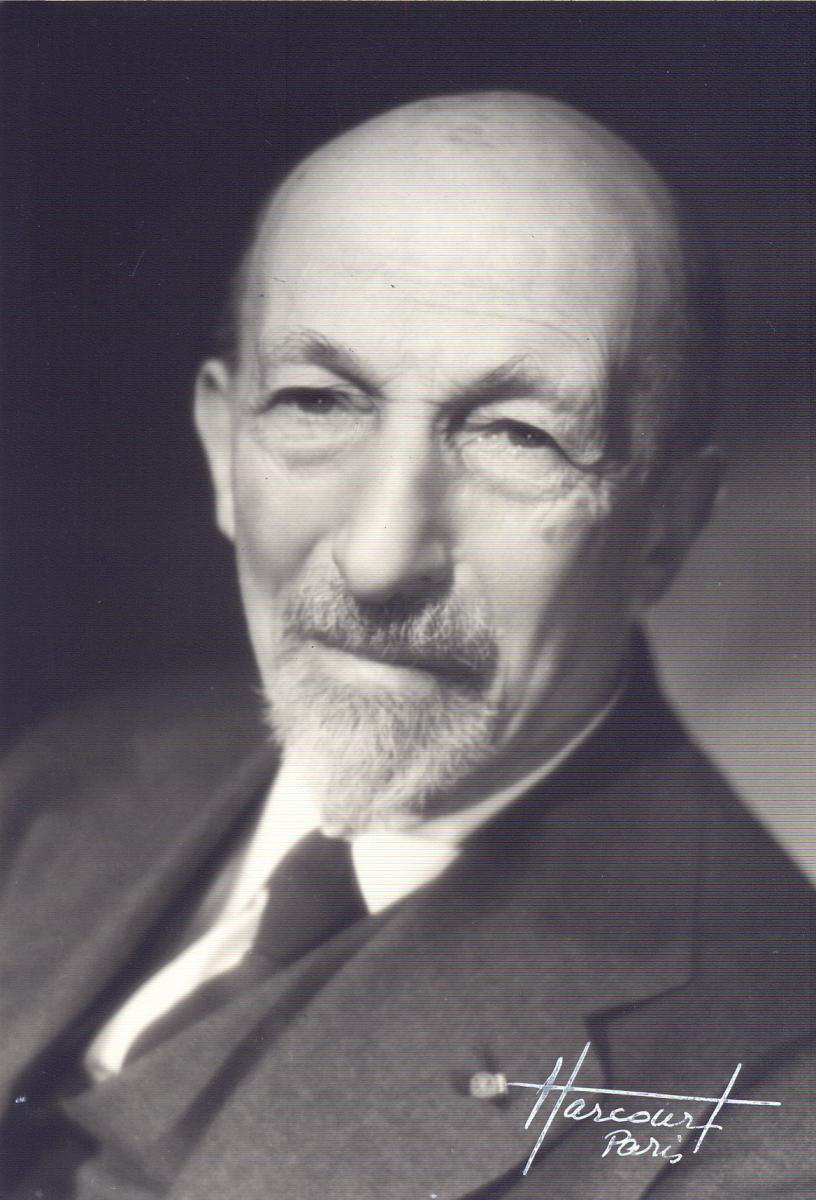
\includegraphics[width=5cm]{images/jacques_hadamard.jpg}
%    \caption{Jacques \textsc{Hadamard}}
%\end{marginfigure}

\begin{theo}{Inégalité d'\textsc{Hadamard}}
    Soit $M \in \M_n(\C)$ et soient $X_1, \dots, X_n$ ses vecteurs colonnes. Alors,
    $$|\mathrm{det} M | \leqslant \prod_{i=1}^{n} \Vert X_i \Vert$$
    avec égalité si et seulement si la famille $(X_i)_{1 \leqslant i \leqslant n}$ est orthogonale.
\end{theo}

%\begin{marginfigure}[-2cm]
%    \resizebox{6.5cm}{6.5cm}{%
    \begin{tikzpicture}
        \node[block] (gram) {Déterminant \\ de \textsc{Gram}};
        \node[block, right of=s1] (iwasama) {Décomposition \\ d'\textsc{Iwasama}};
        \node[block, below right of=gram] (hadamard) {Inégalité \\ d'\textsc{Hadamard}};
    
        \draw (gram) edge[bend right, above left] node {...} (hadamard);
    
        \draw (iwasama) edge[bend left] node {$M=OT$} (hadamard);
    
    \end{tikzpicture}    
}
%\end{marginfigure}

Voyons deux démonstrations de ce résultat; une première en utilisant la décomposition d'\textsc{Iwasama} et une deuxième le \refthm{inegalite_gram}.

\begin{preuve}
    \begin{itemize}
        \item Si la matrice $M$ n'est pas inversible alors $\det M = 0$ et comme une norme est à valeurs positives, le résultat est immédiat. 
        \item Supposons que $M$ est inversible. D'après la décomposition d'\textsc{Iwasama}, il existe une matrice $O \in \mathscr{O}_n(\C)$ et $T \defeq (t_{i,j})_{1 \leqslant i, j \leqslant n}$, triangulaire supérieure dont les coefficients diagonaux sont strictement positifs telles que $M = OT$. D'après la multiplicité du déterminant, 
        $$\det M = \det(O) \det(T).$$
        Or $\det O = \pm 1$ donc
        \begin{equation} \label{det}
            |\det M | = |\det T | = \prod_{i=1}^{n} |t_{i,i}|.
        \end{equation}
        Par construction, pour tout $i \in \llbracket 1, n \rrbracket, t_{i,i} \defeq \langle X_i, O_i \rangle$ où $O_i$ est un vecteur unitaire. D'après l'inégalité de \textsc{Cauchy}-\textsc{Schwarz}, pour tout $i \in \llbracket 1, n \rrbracket$, 
        $$|t_{i,i}| = |\langle X_i, O_i \rangle | \leqslant \norme{X_i} \underbrace{\norme{O_i}}_{=1}.$$
        Ainsi d'après (\ref{det}), 
        $$|\det(M)| \leqslant \prod_{i=1}^n \norme{X_i}.$$
    \end{itemize}
        \textcolor{red}{cas d'égalité}
\end{preuve}

\begin{preuve}
    \begin{itemize}
        \item Si la matrice $M$ n'est pas inversible, le résultat est immédiat. 
        \item Supposons que $M$ est inversible. On a 
        $$\Trsp{M} M = \Gram(X_1, \dots, X_n),$$ 
        la matrice de \textsc{Gram} de la famille des colonnes de la matrice $M$. 
        En composant cette relation par le déterminant, 
        $$\det(\Trsp{M}M) = \det \big( \Gram(X_1, \dots, X_n) \big) = \det(M)^2 $$
        car $\det(\Trsp{M}) = \det M$.
        D'après le (\ref{inegalite_gram}), 
        \begin{align*}
            \det \Gram(X_1, \dots, X_n) &\leqslant \prod_{i=1}^n \norme{X_i}^2 \\
            \text{soit } \det (M)^2 &\leqslant \prod_{i=1}^n \norme{X_i}^2
        \end{align*}
        En passant à la racine on obtient l'inégalité d'\textsc{Hadamard}.
    \end{itemize}
\end{preuve}

\marginnote[0cm]{
    \begin{kaobox}[frametitle=Parallélotope]
        Soit $(x_1, \dots, x_n)$ une famille libre. Le parallélotope engendré par cette famille est défini par
        $$P \defeq \left\{ x = \sum_{i=1}^n t_i x_i,\ \forall i\ t_i \in [0,1]\right\}.$$
    \end{kaobox}
}

L'inégalité d'\textsc{Hadamard} nous apprend que le volume du parallélotope défini par les vecteurs colonnes est inférieur ou égal au produit des normes de ses vecteurs et il y a égalité si et seulement si la matrice est diagonale, ou encore que le parallélotope est rectangle. 

\begin{prop}{}
    Soient $\mathscr{S}_n ^{++} (\R)$ l'ensemble des matrices réelles d'ordre $n$ symétriques à valeurs propres strictement positives et $A = (a_{i,j}) \in \mathscr{S}_n ^{++} (\R)$. Alors,
    $$\det(A) \leqslant \prod_{i=1}^{n} a_{i,i}.$$
\end{prop}

\begin{exercice}    
\marginnote[0cm]{exercice 4, TD 14 \cite{acamanes}}
\begin{enumerate}
    \item Soit $(\gamma_1, \dots, \gamma_n) \in (\Re)^n$. Montrer que $B = (\gamma_i \gamma_j a_{i,j}) \in \mathscr{S}_n^{++}(\R)$. 
    \item Montrer que $\det(A)^{1/n} \leqslant \frac{\Tr(A)}{n}$. \\
    \emph{On pourra utiliser l'inégalité arithmético-géométrique}.
    
    \marginnote[-2cm]{
    	\begin{kaobox}[frametitle=Inégalité arithmético-géométrique]
            Soient $n \in \Ne$ et $x_1, \dots, x_n$ des réels positifs. Alors, 
            $$\frac{x_1 + \cdots + x_n}{n} \geqslant \sqrt[n]{x_1 \cdots x_n}.$$
            Il y a égalité si et seulement si tous les $x_i$ sont égaux.
        \end{kaobox}
        Pour d'autres inégalités, lire le chapitre 16, p.117 de la deuxième édition de Raisonnements divins (en fr)
    }
    \item Montrer que pour tout $i \in \llbracket 1, n \rrbracket, a_{i,i} > 0$. On pose $\gamma_i = \frac{1}{\sqrt{a_{i,i}}}$. En déduire l'inégalité d'\textsc{Hadamard}.
\end{enumerate}
\end{exercice}


\section{Familles de polynômes orthogonaux}
Soient $I$ un intervalle non vide de $\R$ et $w \in \mathscr{C}(I, \Rpe)$. On suppose que, pour tout entier naturel $n$, $\int_I |x|^n w(x) \d x$ converge. On note
$$\mathscr{H} \defeq \ens[\Bigg]{ f \in \mathscr{C}(I, \R) \tq \int_I f^2 w \text{ converge}}.$$
Pour tout $(P, Q) \in \R[X]^2$, on pose 
$$\langle P, Q \rangle \defeq \int_I P(t) Q(t) w(t) \d t.$$

\subsection{Construction}

\begin{exercice}
    \marginnote[0cm]{Source : \cite{acamanes} \href{https://acamanes.github.io/psi/psi_doc/chap_e13.pdf}{(Exercice 17 Ch 13)}}
    \begin{enumerate}
        \item Montrer que $\langle \cdot, \cdot \rangle$ est un produit scalaire sur $\R[X]$.
        \item Montrer qu'il existe une suite $(P_n)_{n \in \N}$ de polynômes tels que 
        \begin{itemize}
            \item pour tout $n \in \N, \deg P_n = n$,
            \item pour tout $(n, m) \in \N^2, n \not= m, \langle P_n, P_m \rangle = 0$,
            \item pour tout $n \in \N$, $P_n$ est unitaire.
        \end{itemize}
        Soit $n$ un entier naturel.
        \item Montrer que $\Vect(P_0, \dots, P_n) = \R_n[X]$.
        \item Montrer que $P_{n+1} \in \R_n[X]^\perp$.
    \end{enumerate}
\end{exercice}

\begin{solution}
    \marginnote[0cm]{Source : Solution de \cite{acamanes}}
    \begin{enumerate}
        \item 
        \begin{itemize}
            \item[$\rhd$] Montrons que $\langle \cdot, \cdot \rangle$ est bien définie. D'une part, $PQw$ est une fonction continue sur $I$. \\
            De plus, $|PQ| \leqslant \frac{P^2 + Q^2}{2}$. Comme $w$ est à valeurs positives, alors
            $$|PQw| \leqslant \frac{1}{2} \Big[ P^2 w + Q^2 w\Big].$$
            Comme $P^2 w$ et $Q^2 w$ sont intégrables sur $I$, d'après les théorèmes de comparaison, $PQw$ est intégrable sur $I$.
            \item[$\rhd$] $\langle \cdot, \cdot \rangle$ est bien symétrique par commutativité du produit de deux polynômes. 
            \item[$\rhd$] est bilinéaire par linéarité des intégrales convergentes.
            \item[$\rhd$] Soit $P \in \R_n[X]$. Comme $w \geqslant 0$, par croissance de l'intégrale, 
            $$\int_I P(x)^2 w(x) \d x \geqslant 0.$$
            De plus, si $\displaystyle \int_I P^2 w = 0$, comme $P$ est une fonction polynomiale donc continue et $w$ est continue, d'après la positivité de l'intégrale,
            $$\forall t \in I, P(t)^2 w(t) = 0.$$
            De plus, $w$ est à valeurs strictement positives, donc
            $$\forall t \in I, P(t) = 0.$$
            Ainsi, $P$ possède une infinité de racines distinctes et $P$ est le polynôme nul.
        \end{itemize}
        Finalement, $\langle \cdot, \cdot \rangle$ est une forme bilinéaire définie positive, donc elle définit un produit scalaire. 
        \item La famille $(X^n)_{n \in \N}$ est la base canonique de $\R[X]$. En appliquant le procédé d'orthogonalisation de \textsc{Gram}-\textsc{Schmidt} à cette famille, on construit une famille de polynôme $(P_n)_{n \in \N}$ telle que, pour tout $n \in \N$, il existe $(\lambda_0, \dots, \lambda_{n-1}) \in \R^n$ tel que
        $$P_n \defeq X^n + \sum_{j=0}^{n-1} \lambda_j P_j.$$
        Ainsi, pour tout $n \in \N$, $\deg P_n = n$ et $P_n$ est unitaire. \\
        De plus, $(P_n)_{n \in \N}$ est une famille orthogonale et 
        $$\forall (m, n) \in \N^2, m \not= n, \langle P_n, P_m \rangle = 0.$$
        \item D'après le procédé de \textsc{Gram}-\textsc{Schmidt}, pour tout $n \in \N$,
        \begin{align*}
            \Vect(P_0, \dots, P_n) &= \Vect(1, X, \dots, X^n)\\
            &= \R_n[X].
        \end{align*}
        \item Soit $P \in \R_n[X]$. D'après la question précédente, il existe $(\mu_0, \dots, \mu_n) \in \R^{n+1}$ tel que
        $$P = \sum_{k=0}^n \mu_k P_k.$$
        Alors, par linéarité du produit scalaire,
        \begin{align*}
            \langle P_{n+1}, P \rangle &= \sum_{k=0}^n \mu_k \langle P_k, P_{n+1} \rangle \\
            &= 0.
        \end{align*}
        Ainsi, $P_{n+1} \in \R_n[X]^\perp$.
    \end{enumerate}
\end{solution}

\subsection{Racines}

\begin{exercice}
    On note $(\alpha_i)_{i \leqslant i \leqslant k}$ les racines de $P_n$ qui appartiennent à $\mathring{I}$ et qui sont de multiplicité impaire. On pose $Q \defeq \prod\limits_{i=1}^k (X - \alpha_i)$.
    \begin{enumerate}
        \item Majorer le degré de $Q$.
        \item Déterminer le signe de $P_n Q$ sur $I$.
        \item En déduire que $k = n$ et que $P_n$ a toutes ses racines réelles et simples dans $\mathring{I}$.
    \end{enumerate}
\end{exercice}

\begin{solution}
    Nous allons montrer que $P_n$ admet au moins $n$ changements de signe dans $I$. C'est pour cela que nous considérons les racines de multiplicité impaire, ce sont elles qui correspondent aux changements de signe. 
    \begin{enumerate}
        \item Comme $\deg P_n = n$, le polynôme $P_n$ possède au plus $n$ racines réelles distinctes. Ainsi, $\deg Q \leqslant n$.
        \item En notant $a_1, \dots, a_p$ les racines réelles distinctes de $P$, on écrit sous forme irréductible:
        $$P_n = \prod_{i=1}^p (X - a_i)^{r_i} \prod_{i=1}^s (X^2 + b_i X + c_i)^{\ell_i}.$$
        Ainsi, pour tout $i \in \llbracket 1,p \rrbracket$, il existe $d_i \in \R$ non nul tel que
        $$P_n(x) \isEquivTo{a_i} d_i (x - a_i)^{r_i}.$$
        Alors, pour tout $i \in \llbracket 1, k$, il existe $\tilde{d_i} \in \R$ non nul tel que
        $$P_n(x) Q(x) \isEquivTo{\alpha_i} \tilde{d_i} (x - \alpha_i)^{r_i+1}.$$
        Comme $r_i$ est impair, le polynôme $P_nQ$ ne change pas de signe au voisinage de $\alpha_i$. \\
        De plus, si $a_i$ est une racine de $P_n$ de multiplicité paire, alors $P_n$ ne change pas de signe au voisinage de $a_i$, d'après la \textcolor{red}{première} question. \\
        Finalement, $P_nQ$ garde un signe constant sur $I$.
        \item Supposons par l'absurde que $k < n$.  Alors, $Q \in \R_k[X] \subset \R_{n-1}[X]$ et, d'après la question $4.$, $P_n \in \R_{n-1}[X]^\perp$. Alors,
        \begin{align*}
            \langle P_n, Q \rangle &= 0 \\
            \int_I P_n(t) Q(t) w(t) \d t &= 0.
        \end{align*}
        D'après la question précédente, $P_n Q w$ est une fonction continue et de signe constant. Ainsi, d'après la positivité de l'intégrale, $P_n Q w = 0$ sur $I$. Comme $w$ est à valeurs strictement positives,
        $$\forall x \in I, P_n(x) Q(x) = 0.$$
        Ainsi, $P_n Q$ possède une infinité de racines soit $P_n Q = 0$. Or $Q \not= 0$, soit $P_n = 0$, ce qui est absurde. Finalement, $k=n$ \note \marginnote[0cm]{\note $P_n$ a au moins $n$ changements de signe sur $I$; par le théorème des valeurs intermédiaires, $P_n$ a au moins $n$ racines dans $I$ et comme $P_n$ est de degré $n$, il y a exactement $n$ racines simples.} et $\deg Q = n$, donc toutes les racines de $P_n$ sont simples et appartiennent à $\mathring{I}$. 
    \end{enumerate}
\end{solution}

\subsection{Relation de récurrence}

\begin{exercice}
    \begin{enumerate}
        \item Montrer que $(P_0, \dots, P_{n-1}, X P_{n-1})$ forme une base de $\R_n[X]$. \\
        On note $P_n = \sum\limits_{k=0}^{n-1} \alpha_k P_k + \alpha_n X P_{n-1}$.
        \item Montrer que, pour tout $j \in \llbracket 0, n - 3 \rrbracket, \alpha_j = 0$.
        \item En déduire qu'il existe trois suites réelles $(a_n), (b_n)$ et $(c_n)$ telles que 
        $$\forall n \in \N,\ P_{n+2} = (a_n X + b_n) P_{n+1} + c_n P_n.$$
    \end{enumerate}
\end{exercice}

\begin{solution}
    \begin{enumerate}
        \item $(P_0, \dots, P_{n-1}, X P_{n-1})$ est une famille de $n+1$ polynômes appartenant à $\R_n[X]$ et de degrés échelonnés. Ainsi, $(P_0, \dots, P_{n-1}, X P_{n-1})$ est une base de $\R_n[X]$.
        \item Soit $j \leqslant n-3$. D'après les définitions,
        \begin{align*}
            \langle X P_{n-1}, P_j \rangle &= \int_I t P_{n-1}(t) P_j(t) \d t \\
            &= \langle \underbrace{X P_j}_{\mathclap{\in \R_{n-2}[X]}}, P_{n-1} \rangle.
        \end{align*}
        Or, d'après la question $4.$, $P_{n-1} \in \R_{n-2}[X]^\perp$. \\
        Alors, comme $(P_0, \dots, P_n)$ est orthogonale,
        \begin{align*}
            0 &= \langle P_n, P_j \rangle \\
            &= \sum_{k=0}^{n-1} \alpha_k \langle P_k, P_j \rangle + \langle X P_{n-1}, P_j \rangle \\
            &= \alpha_j \norme{P_j}^2.
        \end{align*}
        Comme $P_j \not= 0$, alors $\alpha_j = 0$.
        \item D'après la question précédente, il existe
        $(\alpha_{n-2}, \alpha_{n-1}, \alpha_n) \in \R^3$ tel que 
        \begin{align*}
            P_n &= \alpha_{n-2} P_{n-2} + \alpha_{n-1} P_{n-1} + \alpha_n X P_{n-1} \\
            &= (\alpha_n X + \alpha_{n-1}) P_{n-1} + \alpha_{n-2} P_{n-2}.
        \end{align*}
        Ainsi, la suite $(P_n)_{n \in \N}$ satisfait une relation de récurrence d'ordre $2$. 
    \end{enumerate}
\end{solution}

\begin{exercice}    
    \marginnote[0cm]{Source : \cite{exos_oraux} p. 155}
    Soient $f \in \mathscr{C}^0(I, \R)$ et $(P_n)_{n \in \N}$ une famille de polynômes orthogonaux. Montrer que $\sum \langle f, P_n \rangle^2$ converge et prouver l'égalité de \textsc{Parseval}:
    $$\forall f \in \mathscr{C}^0(I, \R), \norme{f}^2 = \sum_{n=0}^{+ \infty} \langle f, P_n \rangle^2.$$
\end{exercice}

\begin{solution}
    
\end{solution}

\subsection{Équation différentielle}
\marginnote[0cm]{Source : Polynômes orthogonaux -- Fabien \textsc{Pucci}}

Soient $a$ et $b$ deux fonctions définies sur un intervalle $I \defeq ] \alpha, \beta [$ de $\R$ borné ou non, avec $\alpha > 0$ sur $I$. On se propose d'étudier les valeurs propres de l'opérateur différentiel:
\begin{align} \label{def_T}
    T(y) \defeq ay'' + by'.
\end{align}
On introduit pour cela une fonction résolvante $w$ à valeurs strictement positives sur $I$ qui permet d'écrire l'opérateur $T$ sous une forme dont nous verrons bientôt l'utilité
\begin{align*}
    T(y) &= \frac{1}{w} \big( a w y' \big)' \\
    &= \frac{1}{w} \big( a'w y' + a w' y' + a w y'' \big) \\
    T(y) &= ay'' + a'y' + \frac{aw'}{w}y'.
\end{align*}
En égalisant avec \ref{def_T}, la fonction $w$ doit être solution de l'équation différentielle linéaire du premier ordre:
$$a w' + (a' - b) w = 0,$$
donc de la forme $w = \e^A$, où $A$ est une primitive de $\frac{b-a'}{a}$. \\
On voit alors que pour le produit scalaire $\langle f, g \rangle \defeq \int_I f(x) g(x) w(x) \d x$, on a:
$$\langle T(f), g \rangle = \int_I (a w f')'(x) g(x) \d x = \big[ a w f' g \big]_I - \int_I a(x) w(x) f'(x) g'(x) \d x.$$
Si de plus la fonction $a w$ s'annule aux bornes de $I$ (ou tend vers $0$ en ses bornes si $I$ est infini), on a par intégration par parties
$$\langle T(f), g \rangle = - \int_I a(x) w(x) f'(x) g'(x) \d x = \langle f, T(f) \rangle,$$
autrement dit, l'opérateur $T$ est symétrique. \\
Bien sûr, il faudrait préciser un peu les hypothèses sur les fonctions $a$ et $b$ pour que tout cela ait un sens, et en particulier préciser sur quel domaine est défini le produit scalaire précédent. \\
Nous nous limiterons ici au cas où $a$ et $b$ sont des fonctions polynomiales de la forme
$$a(x) \defeq a_2 x^2 + a_1 x + a_0 \quad \text{et} \quad b(x) \defeq b_1 x + b_0.$$
Dans ce cas, l'opérateur $T$ est, pour tout entier $n \in \N$, une application linéaire de l'espace $\mathscr{P}_n$ des fonctions polynomiales de degré inférieur à $n$ dans lui-même et le produit scalaire $\langle \cdot, \cdot \rangle$ est défini sur cet espace si $\int_I |x|^k w(x) \d x$ converge pour tout $k \leqslant n$. \\
Sous cette hypothèse, $\mathscr{P}_n$ muni de ce produit scalaire est un espace vectoriel euclidien de dimension finie $n + 1$, et l'opérateur $T$ est un endomorphisme symétrique de cet espace. Il existe alors une base orthonormée de $\mathscr{P}_n$ constituée de vecteurs propres de $T$. \\
En particulier, il existe au moins un vecteur propre $P_n$ de degré $n$, qu'on peut choisir unitaire, et qui vérifie donc:
$$T(P_n) = \lambda_n P_n \Longleftrightarrow a P_n'' + b P_n' = \lambda_n P_n.$$
En considérant le terme de degré $n$ dans cette égalité, on obtient:
$$\lambda_n = n \big( a_2(n-1) + b_1 \big).$$
On sait que les sous-espaces propres d'un endomorphisme symétrique associés à des valeurs propres distinctes sont orthogonaux. Il en résulte qui si les valeurs propres $\lambda_n$ sont toutes distinctes, les polynômes $P_n$ seront deux à deux orthogonaux i.e.
$$\int_I P_n(x) P_n(x) w(x) \d x = 0 \text{ pour } m \not= n.$$
Ce sera le cas si l'équation:
$$a_2 n (n-1) + b_1 n = a_2 m (m-1) + b_1 m \iff (n-m) \big( a_2 (n+m-1) + b_1 \big) = 0$$
n'admet pas de solutions entières positives $(n, m)$ avec $n \not= m$.

\begin{remarque}
    On peut bien sûr ajouter à l'opérateur $T$ un terme $cy$, avec $c$ constant, sans changer la symétrie de $T$, ni les vecteurs propres. On en fait alors que translater les valeurs propres.
\end{remarque}

\subsection{Conclusion}

Pour chaque choix de $w$, on construit ainsi un produit scalaire appelé \emph{produit scalaire usuel avec poids $w$} sur $\mathscr{C}^0(I, \R)$. Pour chacun de ces choix, l'orthogonalisation de \textsc{Gram}-\textsc{Schmidt} appliqué à la base canonique $(1, X, X^2, \dots)$ fait apparaître des familles de polynômes orthogonaux. \\
C'est ainsi qu'il existe beaucoup de familles connues de polynômes orthogonaux dont l'introduction a été motivée par la résolution d'équations différentielles issues de la physique. Ces familles de polynômes sont aussi utilisées, via les formules de quadrature, pour calculer des valeurs approchées d'intégrales. \\
Le tableau ci-dessous rassemble quelques exemples de ces familles. 

\begin{figure*}[h!]
    % \setlength sets the horizontal (column) spacing
    % \arraystretch sets the vertical (row) spacing
    \begingroup
    % \setlength{\tabcolsep}{10pt} % Default value: 6pt
    \renewcommand{\arraystretch}{1.2} % Default value: 1
    \begin{tabular}{|c|c|c|c|c|}
        \hline
        Nom & $I$ & $w(x)$ & Relation de récurrence & Équation différentielle\\
        \hline \hline
        \textsc{Legendre} & $[-1, 1]$ & $1$ & $(n+2) \Leg_{n+2} = (2n+3) \Leg_{n+1} - (n+1)\Leg_n$ & $(1-x^2) y'' - 2xy' + n(n+1) y = 0$\\
        \hline
        \textsc{Tchebychev} & $]-1, 1[$ & $\frac{1}{\sqrt{1-x^2}}$ & $\Tcheby_{n+2} = 2X \Tcheby_{n+1} - \Tcheby_n$ & $(1-x^2)y'' - xy' + n^2y = 0$ \\
        \hline
        \textsc{Laguerre} & $\Rp$ & $\e^{-x}$ & $(n+2) \Lag_{n+2} = (-X+2n+3) \Lag_{n+1} - (n+1) \Lag_n$ & $xy'' + (1-x)y' + ny = 0$\\
        \hline
        \textsc{Hermite} & $\R$ & $\e^{-x^2}$ & $\Hermite_{n+2} = 2X \Hermite_{n+1} - 2(n+1) \Hermite_n$ & $y'' - 2xy' + 2ny = 0$\\
        \hline
    \end{tabular}
    \endgroup
    % The \begingroup ... \endgroup pair ensures the separation
    % parameters only affect this particular table, and not any
    % sebsequent ones in the document.
\end{figure*}


% \section{Polynômes orthogonaux associés à un poids}
% \begin{defi}{}
    Soit $E = \mathscr{C}^0 ([-1, 1], \R)$ et $w$ continue et intégrable sur $]-1, 1[$, vérifiant pour tout $ t \in ]-1, 1[,\ w(t) > 0$. On définit: 
    $$\forall (f,g) \in E^2,\ \langle f, g \rangle = \int_{-1}^{1} f(t)g(t)w(t) \d t.$$
\end{defi}

% \section{Polynômes de \textsc{Legendre} (bis)}
% $$\forall n \in \N, \Leg_n(X) = \frac{1}{2^n n!} U_n^{(n)}(X)$$
où $U_n(X) = (X^2-1)^n$.

\begin{enumerate}
    \item Montrer que $(\Leg_n)_{n \in \N)}$ est une famille orthogonale. \\
    $-1$ et $+1$ sont des racines d'ordre $n$ de $U_n$ donc:
    $$\forall i \in \llbracket 1, n-1 \rrbracket,\ U_n^{(n)}(-1) = U_n^{(n)}(1) = 0 \quad (*)$$
    On calcule $\int_{-1}^{1} U_n^{(n)}(t) \times U_m^{(m)}(t)\d t$ en faisant une \textbf{intégration par parties} un intégrant $U_m^{(m)}$. D'après $(*)$, le crochet est nul. On répète l'opération $n+1$ fois. On obtient alors en facteur dans l'intégrande $U_n^{(2n+1)} = 0$ car $\mathrm{deg}(U_n) = 2n$.
\end{enumerate}

\section{Rayon spectral d'une matrice} \label{rayon_spectral}
\begin{defi}
    Soient $n \geqslant 2, M \in \M_n(\C)$. On définit son \emph{rayon spectral}:
    $$\rho(M) \defeq \max \{ |\lambda |,\ \lambda \in \Sp_{\C}(M) \}.$$
\end{defi}

\section{Caractétisation des projecteurs orthogonaux}
\begin{prop}
    Soient $E$ un espace euclidien et $p$ un projecteur de $E$. Alors $p$ est un projecteur orthogonal si et seulement si, pour tout $x \in E$,
    $$\norme{p(x)} \leqslant \norme{x}.$$
\end{prop}

\begin{preuve}
    \begin{itemize}
        \item $(\Rightarrow)$ Il existe $F$ un sev de $E$ tel que $p$ soit la projection sur $F$ parallèlement à $F^\perp$. On décompose tout vecteur de $E$ comme la somme unique d'un élément de $F$ et de $F^\perp$ puis on applique le théorème de \textsc{Pythagore}. 
        \item $(\Leftarrow)$ 
        \begin{itemize}
            \item (Exos incontournables SUP) Raisonner par l'absurde. Soit $F$ et $G$ tels que $p$ soit la projection sur $F$ parallèlement à $G$. Considérer un vecteur de $G^\perp\ \backslash\ F$ et aboutir à une contradiction.
            \item (Ellipses p.176) Soit $p$ une projection telle que pour tout $x \in E, \norme{p(x)} \leqslant \norme{x}$. \\
            Nous allons poser un vecteur \say{ variable }.
            \marginnote{$p(x+ty) = ty$}
            Soit $x \in \Ker p$ et $y \in \Im p$, pour tout $t \in \R$, 
            \begin{align*}
                \norme{ty} \leqslant \norme{x + ty} &\Leftrightarrow t^2 \norme{y}^2 \leqslant \norme{x+ty}^2 \\
                &\Leftrightarrow t^2 \norme{y}^2 \leqslant \norme{x}^2 + t^2 \norme{y}^2 + 2t \langle x, y \rangle \\
                &\Leftrightarrow \norme{x}^2 + 2t \langle x, y \rangle \geqslant 0 \\
                &\Rightarrow \langle x, y \rangle = 0 \text{ car cette inégalité est vraie pour tout } t \in \R
            \end{align*}
            Donc $\Ker p$ et $\Im p$ sont orthogonaux et $p$ est un projecteur orthogonal.
        \end{itemize}
    \end{itemize}
\end{preuve}

% \begin{marginfigure}[-4cm]
    % % \tdplotsetmaincoords{70}{200}

% \end{marginfigure}


\section{Famille obtusangle}
\begin{defi}
    Soit $E$ un espace euclidien de dimension $n \geqslant 2$. Soit $(x_1, \dots, x_p)$ une famille de vecteurs de $E$. On dit que cette famille est \emph{obtusangle} si et seulement si pour tout $i \not= j, \langle x_i, x_j \rangle < 0$. 
\end{defi}

\begin{exercice0}
    Soit $E$ un espace vectoriel de dimension $n$ et soit $(x_1, \dots, x_p)$ une famille obtusangle de $E$. Montrer que $p \leqslant n + 1$. 
\end{exercice0}


\section{Exercice 6.28 du ELLIPSES}
\begin{exercice}
    Soit $A \in \M_{1,n} (\R)$. Montrer que $B = A^\top A$ est diagonalisable et déterminer une matrice diagonale semblable à $B$.
\end{exercice}

\begin{solution}
    \begin{itemize}
        \item On montre facilement que $B$ est symétrique et comme cette matrice est réelle, elle est diagonalisable.
        \item Toutes les lignes de $B$ sont proportionnelles, et colinéaires à $A$; donc $B$ est de rang $1$ et $\dim E_0(B) = n-1$; la deuxième valeur propre de $B$ est: $\mathrm{Tr}(B) = \sum\limits_{k = 1}^{n} a_k^2$ en posant $A = (a_1, \dots, a_n)$. Enfin, $\Diag \left(\sum\limits_{k = 1}^{n} a_k^2, 0, \dots, 0 \right)$ est semblable à $B$.
    \end{itemize}
\end{solution}


\section{Exercice}
\begin{exercice}
    \marginnote[0cm]{Source : RMS 132 3. Agrégation Interne de Mathématiques (première épreuve 2022)}
    Vrai ou faux: \say{ les matrices carrées et symétriques à coefficients dans $\C$ sont diagonalisables. }
\end{exercice}

Commençons par démontrer le lemme suivant.

\begin{lemme} \lablemme{a_completer}
    Une matrice nilpotente non nulle n'est pas diagonalisable.
\end{lemme}
    
\begin{preuve}
    Soit $A \in \M_n(\R)$ une matrice nilpotente diagonalisable. \\
    Alors il existe $P \in \Gl_n(\R)$ et $D$ une matrice diagonale telles que $A = PD\Inv{P}$. Or $A$ est nilpotente donc il existe $p \in \N$ tel que $A^p = P D^p \Inv{P} = 0$. Donc $D^p = 0$ soit $D = 0$ et $A = 0$. \\
    On peut aussi dire qu'une matrice ayant une unique valeur propre (comme c'est la cas des matrices nilpotentes) est diagonalisable si et seulement si elle est diagonale.
\end{preuve}

\begin{solution}
    Cette affirmation est fausse. \\
    En effet en taille $2$, la matrice $A \defeq \begin{pmatrix}
        1 & \i \\
        \i & -1
    \end{pmatrix}$ est symétrique et non nulle; elle vérifie $A^2 = 0$. Or d'après le lemme, une matrice nilpotente non nulle n'est pas diagonalisable. En taille $n > 2$ la matrice $B$ telle que $[B]_{i,j} = [A]_{i,j}$ si $1 \leqslant i, j \leqslant 2$ et $[B]_{i,j} = 0$ sinon est elle aussi symétrique, nilpotente et non nulle et n'est donc n'est pas diagonalisable. 
\end{solution}   

\marginnote[-2cm]{
    $$
    B \defeq
    \begin{pmatrix}
    1 & \i & 0 & \cdots & 0 \\
    \i & -1 & 0 & \cdots & 0 \\
    0 & 0 & 0 & \cdots & 0 \\
    \vdots & \vdots & \vdots & \ddots & \vdots \\
    0 & 0 & 0 & \cdots & 0
    \end{pmatrix}
    $$
}

A rajouter:
\begin{itemize}
    \item Extremums d'une fonction sur les fonctions continues
    \item Racine carrée d'un endomorphisme autoadjoint positif
    \item Endomorphismes et matrices antisymétriques
\end{itemize}
\chapter{Espaces vectoriels normés, suites}
\labch{espaces_vectoriels_normes_suites}

\section{\texorpdfstring{$\me$}{e} est irrationnel}
\begin{prop}{}
    Le nombre $\e \defeq \exp(1)$ est irrationnel.
\end{prop}
\marginnote[0cm]{Une version de la preuve est dans Proofs from the BOOK (p.47)}
La démonstration suivante est due à Joseph \textsc{Fourier} (1815).
\begin{preuve}
    Supposons par l'absurde qu'il existe deux entiers $a$ et $b$ non nuls tels que $\e = \frac{a}{b}$. Alors, pour tout $n \geqslant 0$,
    $$n! b\, \e = n!\, a.$$
    Le terme de droite est un entier et le terme de gauche s'écrit \note \marginnote[0cm]{$\displaystyle \note\ \e = \sum_{n=0}^{+ \infty} \frac{1}{n!}$}
    $$n! b \left(1 + \frac{1}{1!} + \frac{1}{2!} + \cdots + \frac{1}{n!} + \frac{1}{(n+1)!} + \cdots \right)$$
    qui se décompose en la somme d'un entier
    $$b n! \left(1 + \frac{1}{1!} + \frac{1}{2!} + \cdots + \frac{1}{n!} \right)$$
    et d'un second membre
    $$b \left( \frac{1}{n+1} + \frac{1}{(n+1)(n+2)} + \frac{1}{(n+1)(n+2)(n+3)}+ \cdots \right).$$
    Or ce second membre n'est pas entier car pour $n > 1$,
    \begin{align*}
        0 &< \frac{1}{n+1} + \frac{1}{(n+1)(n+2)} + \frac{1}{(n+1)(n+2)(n+3)} + \cdots \\
        & < \frac{1}{n+1} + \frac{1}{(n+1)^2} + \frac{1}{(n+1)^3} + \cdots = \frac{1}{n+1} \cdot \frac{1}{1-\frac{1}{n+1}} = \frac{1}{n}.
    \end{align*}
    Ainsi le membre de gauche n'est pas entier et on aboutit à une contradiction. On en déduit que le nombre $\e$ est irrationnel.
\end{preuve}

\marginnote{
J. \textsc{Liouville} montre en 1840 que $\e^2$ est également irrationnel. (à compléter)
Charles \textsc{Hermite} montre en 1873 que $\e$ est \emph{transcendant}
\begin{defi}{Nombre transcendant}
\end{defi}
}

\section{Lemme de \textsc{Cesàro}, application à \texorpdfstring{$u_{n+1}=\sin(u_n)$}{u_n+1 = sin(u_n)}}
\marginnote[0cm]{\cite{exos_oraux} p. 227}
\begin{exercice}
    Déterminer une suite simple, équivalente à la suite définie par $u_0 \in ]0, 1]$ et pour tout $n \in \N$,
    $$u_{n+1} = \sin u_n.$$
\end{exercice}

\begin{elem_sol}
    On pourra déterminer $\alpha \in \R$ tel que $u_{n+1}^\alpha - u_n^\alpha$ est convergente vers une limite non nulle, puis appliquer le lemme de \textsc{Cesàro}.
\end{elem_sol}

\section{Une variante de \textsc{Cesàro}}
\begin{exercice}
    Soit $(u_n)_{n \in \N}$ une suite réelle convergeant vers $\ell$. On définit une suite $(v_n)_{n \in \N}$ par 
    $$\forall n \in \N, v_n = \frac{1}{2^n} \sum_{k=0}^{n} \binom{n}{k} u_k.$$
    Montrer que $\displaystyle \lim_{n \rightarrow + \infty} v_n = \ell$.
\end{exercice}

\begin{elem_sol}
    Le méthode consiste à se ramener au cas où $\ell = 0$ en posant deux suites auxiliares $u_n'=u_n - \ell$ et $v_n' = v_n - \ell$. La démarche est en suite analogue à la démonstration du \nameref{lemme_cesaro}.
\end{elem_sol}


\section{Normes de \textsc{Hölder}}
Deux résultats: une norme sur $\K^n$ et une généralisation de l'inégalité de \textsc{Cauchy}-\textsc{Schwarz}. 
\begin{defi}
    Soit $\bm{v} \in \K^n$. Pour tout réel $p \geqslant 1$, l'application $\Vert \bm{\cdot} \Vert_p$ définie par
    $$\Vert \bm{v} \Vert_p = \left (\sum_{k=1}^{n} |v_i|^p \right)^{1/p}$$
    est une norme sur $\K^n$.
\end{defi}

\begin{prop}
    Soient deux réels $p > 1$ et $q > 1$ tels que $\frac{1}{p} + \frac{1}{q} = 1$ ($p$ et $q$ sont \emph{conjugués}). Pour tout $\bm{u}, \bm{v} \in \K^n$
    $$\sum_{k=1}^{n} |u_k v_k| \leqslant \Vert \bm{u} \Vert_p \Vert \bm{v} \Vert_q.$$
\end{prop}

\begin{preuve}(lire aussi \emph{Chapitre 4 - Normes} page 39 \cite{matrices}) \\
    Exercice 4.81 page 377 \cite{oraux_x_ens_3}.
    \begin{enumerate}
        \item Prouver que pour tous $a \geqslant 0, b \geqslant 0: ab \leqslant \frac{a^p}{p} + \frac{b^q}{q}$.
        \begin{itemize}
            \item Utiliser l'\textbf{inégalité de convexité de l'exponentielle}.
        \end{itemize}
        \item Démontrer l'inégalité de \textsc{Hölder}.
        \begin{itemize}
            \item Poser $u'_k = \frac{u_k}{\Vert \bm{u} \Vert_p}$ et $v'_k = \frac{v_k}{\Vert \bm{v} \Vert_p}$ et appliquer le résultat précédent. 
        \end{itemize}
        \item Montrer que $\Vert \bm{\cdot} \Vert$ définit une norme sur $\K^n$.
        \begin{itemize}
            \item Inégalité triangulaire: écrire 
            $$|u_k + v_k|^p = |u_k| \times |u_k + v_k|^{p-1} + |v_k| \times |u_k + v_k|^{p-1}$$ 
            et sommer pour $k$ allant de $1$ à $n$. Appliquer le résultat précédent à chaque somme, factoriser et multiplier l'inégalité par une somme judicieuse. 
        \end{itemize}
    \end{enumerate}
\end{preuve}     

\begin{box_titre}{Proposition 4.1.3. \cite{matrices}}
    Toutes les normes de $E = \K^n$ sont équivalentes. Par exemple:
    $$\Vert x \Vert_\infty \leqslant \Vert x \Vert_p \leqslant p^{1/p} \Vert x \Vert_\infty$$
\end{box_titre}





\pagelayout{wide}
\addpart{Analyse}
\pagelayout{margin}

\chapter{Suites \& Séries numériques}
\labch{suites_et_series_numeriques}

\textsl{
Bien avant qu'elle ne soit conceptualisée, on a utilisé des itérations où est sous-jacente la notion de suite. Par exemple, \textsc{Archimède} quand il cherche une valeur approchée de $\pi$ considère les suites $(p_n)$ et $(P_n)$ des périmètres des polygones inscrits et circonscrits à un cercle de rayon $1$ et aboutit à des formules qui équivalent à $p_{2n} = \sqrt{p_n P_n}$ et $P_{2n} = \frac{2 P_n p_{2n}}{p_{2n} + P_n}$. \\
La théorie des suites au sens moderne est établie au début au début du \textsc{xix}$^\e$ siècle quand s'affirme la volonté de donner à l'analyse des bases rigoureuses qui la débarrassent des notions métaphysiques d'infiniment petits ou de quantités évanouissantes. Dans ses \emph{Notions fondamentales de la théorie des suites}, rédigée vers 1800 et restées inédites, \textsc{Gauss} donne la définition moderne d'une suite (application de $\N$ dans $\R$). Il définit les notions de majorant et de borne supérieure d'une suite. Plus intéressant encore, il donne les définitions de la limite supérieure et de la limite inférieure d'une suite ($\lim \sup a_n = \lim\limits_{n \to + \infty} \sup\limits_{p \geqslant n} a_p$ et $\lim \inf a_n = \lim\limits_{n \to + \infty} \inf\limits_{p \geqslant n} a_p$, dans le langage d'aujourd'hui) et, quand ces deux quantités sont égales, appelle leur valeur commune la limite de la suite. \\
C'est le \emph{Cours d'analyse} de \textsc{Cauchy} (1821) qui ouvre la voie à l'analyse moderne. Dans le chapitre des \emph{Préliminaires}, il donne les définitions d'une suite et de la limite d'une suite, les premières définitions précises de $+\infty$ et $-\infty$, introduit la notion de valeur d'adhérence. Le \say{ critère de \textsc{Cauchy} } de convergence, déjà connu de \textsc{Bolzano} est explicité pour les séries. \\
Pendant une grande partie du \textsc{xix}$^\e$ siècle, la convergence d'une suite de \textsc{Cauchy} ou d'une suite croissante majorée sont présentés comme des axiomes qui constituent le fondement de toutes les questions où intervient la notion de limite. Ce point de vue va être remis en cause par \textsc{Méray} (1868) puis par \textsc{Cantor} (1872) qui, voulant en donner des justifications précises, contruisent $\R$ à partir des suites de \textsc{Cauchy} de $\Q$. \\
La théorie des suites réelles dont tous les concepts sont parfaitement définis depuis la fin du \textsc{xix}$^\e$ a connu récemment des développements importants avec l'étude des systèmes dynamiques, qui apportent un regard nouveau sur les suites définies par une relation de récurrence de la forme $u_{n+1} = f(u_n)$. Si la fonction $f$ est continue et si la suite converge, sa limite $\ell$ est nécessairement un point fixe de $f$. Ce fait, démontré par \textsc{Cauchy}, est à la base de toutes les méthodes numériques itératives. L'intérêt pour telles suites est ancien. Dans le traité \emph{De la méthode des fluxions et des suites infinies} (1740), pour obtenir une valeur approchée d'une solution de l'équation $g(x) = 0$. \textsc{Newton} expose ce qu'on appelle depuis \say{ méthode de \textsc{Newton} }: prenant $a_0$ proche de la solution de l'équation, on considère une suite vérifiant 
$$a_{n+1} = a_n - \frac{g(a_n)}{g'(a_n)}.$$
\begin{marginfigure}[-5cm]
    \centering
    % https://tex.stackexchange.com/questions/549225/how-to-make-tangents-on-figure-like-this
\begin{tikzpicture}[scale=0.8, >=stealth,
    declare function={f(\x)=-0.35+5*exp(\x/2)/exp(3);
        fprime(\x)=2.5*exp(\x/2)/exp(3);},
    dot/.style={circle,fill,inner sep=1pt},
    every pin edge/.style={thin}, scale=0.8]
  \path (0,0) coordinate[label=below left:{$O$}] (O)
     (0,5) coordinate (y) (6,0) coordinate (x);
  \draw[-latex,name path=x-axis] (-0.5,0) --  (x) node[below] {$x$};
  \draw[-latex] (0,-0.5) --  (y) node[left] {$g(x)$};
  \draw[semithick,cyan,name path=curve] plot[variable=\x,domain=0.1:6,smooth]
   (\x,{f(\x)}) (5.8,{f(6)});
  \draw[red,dashed] (5.5,0) coordinate(x0) -- (5.5,{f(5.5)}) coordinate(p0)
  ($(p0)+(-1,{-1*fprime(5.5)})$) coordinate(p0');
  \draw[red,dashed] (intersection of p0--p0' and O--x) coordinate (x1)
  let \p1=(x1) in \pgfextra{\pgfmathsetmacro{\myx}{\x1/1cm}}
  (x1) -- (\myx,{f(\myx)}) coordinate(p1)
  ($(p1)+(-1,{-1*fprime(\myx)})$) coordinate(p1');
  \draw[red,dashed] (intersection of p1--p1' and O--x) coordinate (x2)
  let \p1=(x2) in \pgfextra{\pgfmathsetmacro{\myx}{\x1/1cm}}
  (x2) -- (\myx,{f(\myx)}) coordinate(p2)
  ($(p2)+(-1,{-1*fprime(\myx)})$) coordinate(p2');
  \path (intersection of p2--p2' and O--x) coordinate (x3)
    (x3) node[draw,label=below:{$a_{3}$}] {}
  foreach \X [count=\Y] in {0,...,2}
   {(x\X) node[draw,label=below:{$a_{\X}$}] {}
    (x\Y) edge[red,shorten >=-1em,shorten <=-1ex] (p\X)
   \ifnum\X=0   
   (p\X) node[dot,cyan,label={[black]left:{$\big(a_{\X},g(a_{\X}) \big)$}}] {}
   \else
   (p\X) node[dot,cyan,pin={[black]90:{$\big( a_{\X},g(a_{\X}) \big)$}}] {}
   \fi 
   };
  \path[name intersections={of=curve and x-axis,by=i}]
   (i) node[cyan,draw,fill,
   ,pin={[black,align=center]90: point\\ \contour{white}{recherché}}](in){};  
 \end{tikzpicture}

    \caption*{\centering Illustration de la méthode de \textsc{Newton}}
\end{marginfigure}
C'est lors de l'étude de certains systèmes dynamiques discrets \footnote{Qui revient à l'étude du comportement des applications itérées $f^n : X \to X$.} qu'est apparue la notion de chaos, qui a connu ces dernières décennies un grand succès. Pour des fonctions $f$ très simples (par exemple une fonction trinôme), le système dynamique peut avoir un comportement qui semble aléatoire. L'exemple le plus connu est la \emph{suite logistique} vérifiant une relation de la forme
$$u_{n+1} = (1 + \alpha) u_n - \alpha u_n^2.$$
Cette suite a été utilisée par \textsc{Verhulst} en 1845 pour décrire un modèle de croissance de la population. Pour $0 < \alpha \leqslant 2$ et une population $u_0$ pas trop importante, la suite $(u_n)$ converge vers la population stable $1$. Mais comme l'a démontré en 1963 le météorologiste $\textsc{E. N. Lorenz}$, pour des valeurs plus grandes de $\alpha$, cette loi décrit certains aspects des flux turbulents. \\
Dans les années 1980, de grands progrès ont été accomplis dans l'étude de ces systèmes dynamiques grâce à la puissance des ordinateurs. Par exemple, pour la suite logistique, on observe que, pour $2 < \alpha < 2,5$, le comportement de la suite tend vers une oscillation régulière entre deux valeurs (cycle d'ordre $2$); puis pour $2,5 \leqslant \alpha < 2,55$, vers un cycle d'ordre $4$; ensuite quand $\alpha$ augmente, vers des cycles d'ordres $8, 16, \dots$ Au-delà de $2,57$ environ, le système devient chaotique. \textsc{Feigenbaum} a montré en 1981 que, pour une classe assez large d'applications $f$ de $[-1, 1]$ dans $[-1, 1]$ et $f_\lambda = \lambda f, 0 < \lambda < 1$, le système dynamique défini par $u_{n+1} = f_\lambda(u_n)$ a un comportement comparable: il existe une suite croissante de valeurs $\lambda_j$ du paramètre $\lambda$ pour lesquelles la dynamique change (le nombre de points d'un cycle double quand $\lambda$, supposé passage de $\lambda_j$) jusqu'à une valeur critique $\lambda_\infty$, de telle manière que $\frac{\lambda_{j+1} - \lambda_j}{\lambda_{j+2} - \lambda_{j+1}}$ tende vers $\delta = 4,669\dots$, constante universelle indépendante de $f$. Au-delà de $\lambda_\infty$, on retrouve des cycles stables de période $3 \cdot 2^j$ et des points de bifurcation. \\
On s'est aussi intéressé à l'itération de fonction complexes, en particulier les fonction $f : x \mapsto x^2 + c$, où $c \in \C$. On étudie l'ensemble des nombres complexes $z$ pour lesquels la suite de premier terme $z$ est bornée. On note $K_c$ cet ensemble, et on l'appelle \emph{ensemble de \textsc{Julia}}. Sa frontière présente des formes très belles et très variés selon les valeurs de $c$. Les premiers résultats, établis entre 1905 et 1920, sont dus à \textsc{Fatou} et \textsc{Julia} (évidemment sans aucun moyen informatique). En 1980, \textsc{Mandelbrot} étudia l'ensemble des points $c$ pour lesquels $0$ est dans $K_c$ (le célèbre \emph{ensemble de \textsc{Mandelbrot}}). 
\begin{marginfigure}[-2cm]
    \centering
    \caption*{\centering L'ensemble de \textsc{Mandelbrot}}
    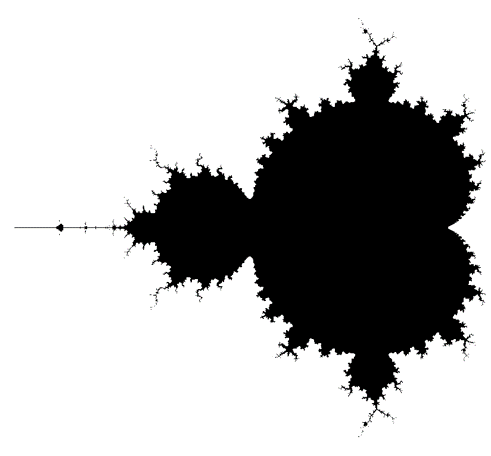
\includegraphics[scale=0.2]{images/ensemble_de_mandelbrot.png}
\end{marginfigure}
Les ensembles de \textsc{Julia} ont les propriétés des fractales, en particulier l'autosimilitude. En revanche, l'ensemble de \textsc{Mandelbrot} est extraordinairement varié: plus l'échelle est grande, plus l'image se complique. On a montré un caractère universel de l'ensemble de \textsc{Mandelbrot}: pour diverses fonctions complexes à un paramètre, on trouve des copies déformées de cet ensemble. 
}

Séries numériques (oraux x-ens)\\
\textsl{
Dans une tentative d'historique des séries numériques, nous pourrions faire remonter leurs origines aux travaux développés dès la fin du \textsc{xvii}$^\e$ siècle autour du comportement asymptotique de sommes du type $\sum\limits_{k=1}^n f(k)$. Quelques années après les travaux de \textsc{Bernoulli} sur ce sujet, \textsc{Euler} et \textsc{Mac-Laurin} produisent indépendamment une \say{ formule sommatoire } obtenue par inversion d'identités tayloriennes:
$$\sum_{k=1}^n f(k) = \int_0^n f + \frac{f(0) + f(n)}{2!} + \frac{f'(n) - f'(0)}{3!} - \frac{f'''(n) - f'''(0)}{6!}\cdots$$
\marginnote[0cm]{
    \note En notant $\mathrm{b}_k$ les nombres de \textsc{Bernoulli},
    $$\sum_{k=0}^{n-1} k^m = \sum_{k=0}^m \binom{m}{k} \mathrm{b}_k \frac{n^{m+1-k}}{m+1-k}.$$
    Pour $|x| < 2 \pi$,
    $$\frac{x}{\e^x-1} = \sum_{k=0}^{+\infty} \mathrm{b}_k \frac{x^k}{k!}.$$
    \note Soit $s \in \Ne$,
    $$\sum_{n=1}^{+\infty} \frac{1}{n^{2s}} = \frac{|\mathrm{b}_{2s}|(2 \pi)^{2s}}{2 (2s)!}.$$
}
Si l'expression générale donnant les coefficients de cette formule leur échappe dans un premier temps, \textsc{Euler} établit leur lien avec les coefficients du développement en série de $\frac{x}{\e^x-1}$ et les nombres de \textsc{Bernoulli}, introduits par celui-ci dans le calcul des sommes $\sum\limits_{k=1}^n k^p$ \note. \textsc{Euler} en déduit, par de jolis calculs, les sommes des séries $\sum\limits_{n=1}^{+\infty} \frac{1}{n^{2s}}$ pour $s$ entier naturel non nul \note.
Cependant, le problème de la convergence des sommes en question n'est jamais au centre de leurs réflexions et l'aspect formel l'emporte, ce qui conduit parfois les plus grands mathématiciens du siècle à commettre de lourdes erreurs. Vers 1768, \textsc{d'Alembert} commence à douter de la validité de l'emploi de séries non convergentes. En 1826, le mot d'\textsc{Abel} illustre parfaitement cette nouvelle préoccupation: \say{ Les séries divergentes sont des inventions du diable, et c'est une honte que l'on ose fonder sur elles la moindre démonstration. On peut en tirer  tout ce qu'on veut quand on les emploie et ce sont elles qui ont produit tant d'échecs et tant de paradoxes } (Œuvres, 1881). \\
Mais ce sont les nécessités du calcul numérique qui imposent vraiment un effort de rigueur dont \textsc{Gauss}, s'étant fait une idée claire de la notion de limite, sera le principal artisan. À partir de là, il paraît naturel d'établir des critères simples de convergence: on en doit plusieurs à \textsc{Cauchy}, et notamment celui qui porte son nom: si la suite de réels positifs $(a_n)_{n \geqslant 0}$ est telle que la limite supérieure de $\sqrt[n]{a_n}$ est strictement inférieure à $1$, alors la série $\sum a_n$ est convergente. \\
(il y a une suite)
}

\newpage

\section{Lemme de \textsc{Cesàro}} \label{lemme_cesaro}
\begin{lemme}
    Soit $(u_n)_{n \in \Ne}$ une suite réelle ou complexe convergeant vers $\ell$.
    Alors la suite de terme général $\frac{1}{n} \sum\limits_{k=1}^{n} u_k$ converge aussi vers $\ell$.
\end{lemme}

\begin{preuve}
    Soit $\varepsilon > 0$. Comme la suite $(u_n)$ converge vers $\ell$, il existe un rang $n_0 \in \Ne$ tel que pour tout $n \geqslant n_0,\ |u_n - \ell| \leqslant \varepsilon$. \\
    Soit $n \geqslant n_0$,
    \begin{align*}
        \left| \frac{1}{n} \sum_{k=1}^n u_k - \ell \right| &= \left| \frac{1}{n} \sum_{k=1}^n (u_k - \ell) \right| \\
        \text{par l'inégalité triangulaire} &\leqslant \frac{1}{n} \sum_{k=1}^n |u_k - \ell| \\
        &\leqslant \frac{1}{n} \Bigg( \underbrace{\sum_{k=1}^{n_0-1} |u_k - \ell|}_{\defeq K} + \sum_{k=n_0}^n \underbrace{|u_k - \ell|}_{\leqslant \varepsilon} \Bigg) \\
        &\leqslant \frac{K}{n} + \varepsilon
    \end{align*}
    Or $\lim\limits_{n \to \infty} \frac{K}{n} = 0$ donc il existe un rang $n_1 \in \Ne$ tel que pour tout $n \geqslant n_1, \left| \frac{K}{n} \right| \leqslant \varepsilon$. \\
    Ainsi pour tout $n \geqslant \max \{ n_0, n_1 \}$, 
    $$\left| \frac{1}{n} \sum_{k=1}^n u_k - \ell \right| \leqslant 2 \varepsilon.$$
    On en déduit que la suite $\Bigg( \frac{1}{n} \sum\limits_{k=1}^{n} u_k \Bigg)_{n \in \Ne}$ converge vers $\ell$.
\end{preuve}

\begin{remarque}
    \textcolor{red}{à réécrire}
    Attention, la réciproque du lemme de \textsc{Cesàro} est fausse. Une suite $(u_n)$ peut converger au sens de \textsc{Cesàro} i.e. $\Bigg( \frac{1}{n} \sum\limits_{k=1}^{n} u_k \Bigg)_{n \in \Ne}$ converge sans pour autant que la suite $(u_n)$ converge. Par exemple, $(u_n) \defeq \left((-1)^n\right)_n$.
\end{remarque}

\section{Constante d'\textsc{Euler}}
\begin{tcolorbox}
    La constante d'\textsc{Euler} $\gamma$ est définie par:
    $$\gamma = \lim_{n \to \infty} \left(\sum_{k=1}^{n} \frac{1}{k} - \ln(n) \right) \approx 0,577 215 664 \dots$$
\end{tcolorbox}

\begin{enumerate}
    \item Poser $v_n = H_n - \ln(n)$
    \item Montrer que $v_{n+1}-v_n = \mathcal{O}\left(\frac{1}{n^2}\right)$\\
    On peut aussi montrer...
    \item ... la décroissance de la suite $(v_n)$. \\
    Soit $n \in \N$. 
    $$v_n - v_{n+1} = \ln(n+1) - \ln(n) - \frac{1}{n+1}$$
    Deux méthodes:
    \begin{itemize}
        \item On transforme $\ln(n+1) - \ln(n)$ en intégrale:
        $$v_n - v_{n+1} = \int_{n}^{n+1} \underbrace{\left( \frac{1}{t} - \frac{1}{n+1} \right)}_{\geqslant 0}\ \d t > 0.$$
        \item D'après le \textbf{théorème des accroissements finis}, il existe $c \in ]n, n+1[$ tel que 
        $$\ln(n+1) - \ln(n) = \ln'(c)((n+1) - n) = \frac{1}{c}$$
        d'où l'on tire que 
        $$v_n - v_{n+1} = \frac{1}{c} - \frac{1}{n+1} > 0.$$
    \end{itemize}
    \item ... que $\boxed{\forall n \in \Ne,\ \ln(n+1) \leqslant H_n \leqslant \ln(n) + 1}$ grâce à l'\textbf{encadrement de l'intégrale} sur $[k, k+1]$ de la fonction $t \mapsto \frac{1}{t}$.
\end{enumerate}

\section{Séries de \textsc{Bertrand}}
\begin{defi}{Séries de \textsc{Bertrand}}
    Soient $\alpha$ et $\beta$ deux réels. On nomme \emph{série de \textsc{Bertrand}} la série de terme général $\displaystyle \frac{1}{n^\alpha \ln^\beta (n)}$ pour $n \geqslant 2$. 
\end{defi}

\begin{theo}{}
    La série de \textsc{Bertrand} converge si et seulement si \begin{cases} \alpha > 1 \\
    \text{ou} \\ \alpha = 1 \text{ et } \beta > 1 \end{cases}.
\end{theo}

\begin{preuve}
    Distinguons trois cas selon les valeurs prises par $\alpha$:
    \begin{enumerate}
        \item[$\rhd$] si $\alpha > 1$, soit $\gamma \in ]1, \alpha[$. Par croissances comparées,
        $$\displaystyle \frac{1}{t^{\alpha} \ln^{\beta} (t)} = o_{+ \infty} \left( \frac{1}{t^{\gamma}} \right).$$
        Or, d'après le théorème de \textsc{Riemann}, la fonction $t \mapsto \frac{1}{t^\gamma}$ est intégrable sur $[2, +\infty[$ car $\gamma > 1$. Ainsi, en appliquant les théorèmes de comparaison, $\int_2^{+ \infty} f$ converge.
        \item[$\rhd$] si $\alpha < 1$, soit $\gamma \in ]\alpha, 1[$.Par croissances comparées,
        $t^{\gamma} f(t) \xrightarrow[t \to + \infty]{} + \infty$
        donc à partir d'un certain rang, $f(t) \geqslant \frac{1}{t^{\gamma}} > 0$. Or, d'après le théorème de \textsc{Riemann}, la fonction $t \mapsto \frac{1}{t^\gamma}$ n'est intégrable pas sur $[2, +\infty[$ car $\gamma < 1$. Ainsi, en appliquant les théorèmes de comparaison (les intégrandes sont positives), $\int_2^{+ \infty} f$ diverge.
        \item[$\rhd$] si $\alpha = 1$, revenons aux intégrales partielles:
        $$\int_{2}^{X} \frac{1}{t \ln^{\beta} (t)} \d t = 
        \begin{cases}
            \left[ \frac{\ln ^{1-\beta} (t)}{1-\beta} \right]_2 ^X & \text{si } \beta \not = 1, \\
            \left[\ln (\ln(t)) \right]_2 ^X & \text{si } \beta = 1.
        \end{cases}
        $$
        On en déduit que l'intégrale de la fonction $t \mapsto \frac{1}{t \ln^{\beta} (t)}$ converge sur $[2, + \infty[$ si et seulement si $\beta > 1$.
    \end{enumerate}
\end{preuve}


\begin{exercice}
    \marginnote[0cm]{\cite{acamanes}}
    On note $h : x \mapsto \sum\limits_{n=2}^{+ \infty} \frac{1}{n^x \ln n}$.
    \begin{enumerate}
        \item Étudier la continuité de $h$ sur son domaine de définition.
        \item Étudier les limites de $h$ aux bornes de son intervalle de définition.
        \item Déterminer des équivalents de $h$ aux bornes de son intervalle de définition.
    \end{enumerate}
\end{exercice}

\begin{solution}
\begin{enumerate}
    On note $f_x : t \mapsto \frac{1}{t^x \ln t}$.
    \item D'après le théorème de \textsc{Bertrand} sur les séries numériques, l'ensemble de définition de $h$ est $\mathcal{D}_h \defeq ]1, + \infty[$. \\
    Soit $a > 1$. On se place sur $I \defeq [a, +\infty[$. Pour tout $x \in I$,
    $$\left| \frac{1}{n^x \ln n} \right| \leqslant \frac{1}{n^\alpha \ln n}$$
    comme $a > 1$, d'après le théorème de \textsc{Bertrand} sur les séries numériques, la série du terme majorant converge et donc par théorème de comparaison, la suite $(f_x)$ converge normalement sur tout segment de la forme de $I$. On en déduit que $h$ est continue sur $\mathcal{D}_h$. 
    \begin{itemize}
        \item En $+ \infty$: comme la série des $f_x$ converge uniformément sur $[2, + \infty[$ (on aurait pu choisir une valeur que $2$), d'après le théorème de la double limite
        $$\lim_{x \to + \infty} h(x) = \sum_{n=2}^{+ \infty} \left[\lim_{x \to +\infty} f_x(n) \right] = 0.$$
        \item En $1^+$: On montre que la fonction $f_x$ est décroissante et donc $h$ aussi. On note $\ell \defeq \lim\limits_{1^+} h$. D'après le théorème de la limite monotone, $\ell \in \R \cup \{ + \infty \}$. \\
        Supponson que $\ell \in \R$, alors
        $$h(x) = \sum_{n=2}^{+\infty} \frac{1}{n^x \ln n} \geqslant \sum_{n=2}^N \frac{1}{n^x \ln n}$$
        et en passant à la limite quand $x$ tend vers $1^+$ dans l'inégalité (ce qui est licite) on obtient
        $$\ell \geqslant \sum_{n=2}^N \frac{1}{n \ln n}.$$
        Nous aboutissons donc à une contradiction car la somme minorante diverge quand $N$ tend vers $+ \infty$. Finalement,
        $$\lim_{1^+} h = + \infty.$$
    \end{itemize}
    \item 
    \begin{itemize}
        \item En $+ \infty$: on intuite que la premier terme de la somme domine les autres. On a
        $$2^x \ln(2) h(x) = 1 + \sum_{n=3}^{+\infty} \left(\frac{2}{n}\right)^x \frac{\ln 2}{\ln n}.$$
        On peut montrer(...) que la somme converge normalement sur $[2, +\infty[$. On en déduit que 
        $$h(x) \isEquivTo{+\infty} \frac{1}{2^x \ln 2}.$$
        \item En $1^+$: un encadrement par la méthode des rectangles permet de trouver
        $$\int_{3}^{+\infty} f_x(t) \d t + \frac{1}{2^x \ln 2} \leqslant h(x) \leqslant \int_{2}^{+\infty} f_x(t) \d t + \frac{1}{2^x \ln 2}.$$
        On en déduit que 
        $$h(x) \isEquivTo{1^+} \int_2^{+\infty} f_x(t) \d t$$
        soit après calculs (...)
        $$h(x) \isEquivTo{1^+} - \ln(x-1).$$
    \end{itemize}
\end{enumerate}
\end{solution}

\section{Deux sommes} \label{deux_sommes}
\begin{exercice}
    Calculer $\displaystyle \sum_{n=1}^{+\infty} \frac{(-1)^n}{n}$ et $\displaystyle \sum_{n=0}^{+\infty} \frac{(-1)^n}{2n+1}$.
\end{exercice}

\begin{elem_sol}
    \begin{itemize}
        \item Exprimer les termes généraux avec une intégrale. 
        \item (1)$= -\ln(2)$, (2)$= \frac{\pi}{4}$.
    \end{itemize}
\end{elem_sol}


\section{Sommation des relations de comparaison} \label{sommation_relations_comparaison}
\begin{tcolorbox}
    Soient $(a_n)_{n \in \Ne}$ et $(b_n)_{n \in \Ne}$ deux suites à valeurs positives telles que $a_n \sim b_n$.\\
    Si $ \sum a_k$ diverge, alors $\sum\limits_{k=1}^{n} a_k \sim \sum\limits_{k=1}^{n} b_k$. \\
    Si $ \sum a_k$ converge, alors $\sum\limits_{k=n+1}^{+ \infty} a_k \sim \sum\limits_{k=n+1}^{+ \infty} b_k$. \\
    \emph{Il y a des résultats analogues si $u_n = o(v_n)$ ou si $u_n = \mathcal{O}(v_n)$.}
\end{tcolorbox}

\begin{itemize}
    \item Revenir à la définition de l'équivalence avec le $o$: $a_n \sim b_n \Longleftrightarrow a_n -b_n = o(b_n)$.
\end{itemize}

\section{Formule de \textsc{Stirling}}
\label{preuve_stirling}
\begin{theo}
    $$n! \sim \left(\frac{n}{\me}\right)^n \sqrt{2 \pi n}$$
\end{theo}

\begin{preuve}
    \begin{enumerate}
        \item Montrer que $\left( \frac{n!\me^n}{\sqrt{n}n^n} \right)_{n \in \Ne}$ converge vers $\ell \in \R$
        \item Montrer que $\ell = \sqrt{2 \pi}$ en utilisant l'\nameref{integrale_wallis}:
        $$\Wallis_n \defeq \int_{0}^{\pi/2}\sin^n(t) \d t$$
        \begin{enumerate}
            \item Montrer que $(\Wallis_n)_{n \in \N}$ est décroissante
            \item Exprimer $\Wallis_{n+2}$ en fonction de $\Wallis_n$ grâce à une IPP: $$(n+2)\Wallis_{n+2} = (n+1)\Wallis_n$$
            \item Exprimer $\Wallis_{2p}$ et $\Wallis_{2p+1}$ en fonction de $p$:\\
            $$\Wallis_{2p} = \frac{\binom{2p}{p}}{2^{2p}}\frac{\pi}{2} \text{ et } \Wallis_{2p+1} = \frac{2^{2p} (p!)^2}{(2p+1)!}$$
            \item Utiliser les points (a) et (b) pour montrer que $\frac{\Wallis_n}{\Wallis_{n+1}} \longrightarrow 1$
            \item Utiliser les points (c) et (d) pour montrer que $\left ( \frac{2^n n!}{n ((2n)!)^2} \right)^4 \longrightarrow \pi$
            \item Utiliser le point 1. pour déterminer $\ell$
        \end{enumerate}
    \end{enumerate}
\end{preuve}

\begin{preuve}
    Calculons $\Wallis_{n+2}$ en effectuant une intégration par parties. On pose $u(t) \defeq - \cos(t)$ et $v(t) \defeq \sin^{n+1}(t)$, toutes deux de classe $\mathscr{C}^1$ sur $\left[0, \frac{\pi}{2} \right]$. 
    \begin{align*}
        \Wallis_{n+2} &= \underbrace{\left[ -\cos(t) \sin^{n+1}(t) \right]_0^{\pi/2}}_{=0} + (n+1) \int_0^{\pi/2} \cos^2 (t) \sin^n(t) \d t \\
        &= (n+1) \int_0^{\pi/2} (1 - \sin^2(t)) \sin^n(t) \d t \\
        &= (n+1) \Wallis_n - (n+1) \Wallis_{n+2} \\
        \text{soit } (n+2) \Wallis_{n+2} &= (n+1) \Wallis_n.
\end{align*}
Soit $p \in \N$. D'après la relation précédente, 
\begin{align*}
    \Wallis_{2p} &= \frac{2p-1}{2p} \Wallis_{2p-2} \\
    &= \frac{2p-1}{2p} \times \frac{2p-3}{2p-2} \times \cdots \times \frac{1}{2} \times \underbrace{\Wallis_0}_{=\pi/2} \\
    &= \frac{\prod\limits_{k=1}^p (2k+1)}{\prod\limits_{k=1}^{p+1} (2k)} \frac{\pi}{2} \\
    &= \frac{\left[\prod\limits_{k=1}^p (2k+1) \right] \times \left[ \prod\limits_{k=1}^{p+1} (2k) \right]}{\left[\prod\limits_{k=1}^{p+1} (2k) \right]^2} \frac{\pi}{2} \\
    \Wallis_{2p} &= \frac{(2p)!}{2^{2p}(p!)^2} \frac{\pi}{2}.
\end{align*}
\begin{align*}
    \Wallis_{2p+1} &= \frac{2p}{2p+1} \Wallis_{2p-1} \\
    &= \frac{2p}{2p+1} \times \frac{2p-2}{2p-1} \times \cdots \times \frac{2}{3} \times \underbrace{\Wallis_1}_{=1} \\
    &= \frac{\prod\limits_{k=1}^p (2k)}{\prod\limits_{k=0}^p (2k+1)} \\
    &= \frac{\left[ \prod\limits_{k=1}^p (2k) \right]^2}{\left[ \prod\limits_{k=0}^p (2k+1) \right] \left[ \prod\limits_{k=1}^p (2k) \right]} \\
    \Wallis_{2p+1} &= \frac{2^{2p}(p!)^2}{(2p+1)!}.
\end{align*}
\end{preuve}


\section{Règle de \textsc{Raabe-Duhamel}}
\begin{theo}
    Soit $\alpha$ un réel et $(u_n)_{n \in \N}$ une suite de réels strictement positifs. On suppose que
    $$\displaystyle \frac{u_{n+1}}{u_n} = 1 - \frac{\alpha}{n} + \mathcal{O} \left( \frac{1}{n^2} \right).$$ Alors $\sum u_n$ converge si et seulement si $\alpha > 1$. 
\end{theo}
\marginnote[-1cm]{Voir exercice 3.43. \cite{oraux_x_ens_3}}
\begin{enumerate}
    \item[($\Rightarrow$)] Montrer que si $u_n=\frac{K}{n^{\alpha}}$ avec $K>0$ et $\alpha > 1$ alors $(u_n)$ vérifie la relation.
    \item[($\Leftarrow$)] Soit $(v_n)$ une suite vérifiant les hypothèses. Montrer qu'il existe $K>0$ tel que $v_n \sim \frac{K}{n^{\alpha}}$ avec $\alpha > 0$. Pour cela, étudier la série de terme général $\ln (v_n)$.
\end{enumerate}

Être capable de donner deux séries montrant qu'on ne peut pas conclure si $\alpha=1$.

\section{Suites sous-additive}
\emph{Exercice 2. TD I \cite{acamanes}}\\

\begin{defi}
    Une suite $(u_n)_{n\geqslant1}$ est dite \emph{sous-additive} si pour tout couple d'entiers non nuls $(n, m)$, $u_{n+m} \leqslant u_n + u_m$.
\end{defi}

\begin{exercice}
    Soit $(u_n)_{n \geqslant 1}$ une suite sous-additive. On pose $b_n = \min\limits_{k \in \llbracket 1, n \rrbracket} \frac{u_k}{k}$.
    \begin{enumerate}
        \item \begin{enumerate}
            \item Soit $\alpha \in \Rp$ et, pour $n \in \Ne, t_n = n^{\alpha}$. Montrer que $(t_n)$ est sous-additive si et seulement si $\alpha \leqslant 1$. Déterminer alors la limite de la suite $(t_n/n)$.
            \item Soit $(w_n)$ une suite réelle telle que pour tout $(n,m) \in (\Ne)^2, w_{n+m} = w_n + w_m$. Montrer que $(w_n)$ est sous-additive et calculer la limite de la suite $(w_n / n)$.
        \end{enumerate}
        \item Montrer qu'il existe $\ell \in \R \cup \{ - \infty \}$ telle que $\lim\limits_{n \to +\infty} v_n = \ell$.
        \item Montrer que pour tout $(m,n) \in (\Ne)^2, u_{nm} \leqslant m u_n$.
        \item On suppose que $\ell \not= - \infty$. Soit $\varepsilon > 0$.
        \begin{enumerate}
            \item Montrer qu'il existe $m \in \N$ tel que $\frac{u_m}{m} \leqslant \ell + \varepsilon$. 
            \item En utilisant le théorème de la division euclidienne, montrer que $\left( \frac{u_n}{n} \right)_{n \geqslant 1}$ converge vers $\ell$.
        \end{enumerate}
    \end{enumerate}
\end{exercice}

\begin{solution}
    1.a)\\ 
    \indent $(\Leftarrow)$ Étudier les cas où $n=m$.\\
    \indent $(\Rightarrow)$ Étudier la fonction $f:x \mapsto 1+x^{\alpha} - (1+x)^{\alpha}$.\\
    1.b)\\
    \indent Étudier le cas où $m=1$ et montrer que $w_n = n w_1$.\\
    2)\\
    \indent Montrer que la suite $(v_n)$ est décroissante.\\ 
    4.b)\\
    \indent Soit $(n, m) \in (\Ne)^2$. D'après le théorème de la division euclidienne, il existe un unique couple $(k, r) \in \Ne \times \llbracket0, m-1 \rrbracket$ tel que $n=km+r$.\\
    \indent Utiliser successivment la définition d'une suite sous-additive et les résultats des questions 3) et 4.a).
\end{solution}


\section{Étude de la suite de terme général \texorpdfstring{$u_n = \left( \frac{1}{b-a} \int_{a}^{b} f(x)^n \d x \right)^{1/n}$}{égal à une intégrale}}
\emph{Exercice 9. TD I}\\
La fonction $f$ est supposée continue et positive sur $[a, b]$.

\begin{itemize}
    \item La démarche générale consiste à encadrer $u_n$. 
    \item \underline{Majoration:} $f$ est continue sur un segment donc est en particuler bornée par un réel positif $M$. On peut montrer que $u_n \leqslant M$ \emph{(ne pas oublier l'argument de la continuité lors du passage à l'intégrale)}.
    \item \underline{Minoration:} soit $\varepsilon > 0$, soit $x_0$ tel que $f(x_0) = M$. Comme $f$ est continue en $x_0$, il existe $[c, d] \subset [a, b]$ tel que $x_0 \in [c, d]$ et pour tout $x \in [c, d]$, $f(x) \geqslant M - \varepsilon$ \emph{(un dessin permet de bien comprendre la stratégie)}.\\
    On peut ensuite montrer que $u_n \geqslant \left(\frac{d-c}{b-a} \right)^{1/n}(M-\varepsilon) \xrightarrow[n \to + \infty]{} M-\varepsilon$.
    \item Finalement, $\boxed{u_n \displaystyle \longrightarrow M = \max_{[ a, b ]} f = \Ninf{f}}$.
\end{itemize}

\section{Transformation d'\textsc{Abel}} \label{transformation_abel}
\marginnote[0cm]{Texte de \cite{oraux_x_ens_3} p. 262.}
La technique des transformations d'\textsc{Abel} peut être vue comme des intégrations par parties discrètes. On s'intéresse à la nature de la série $\sum a_n b_n$ où $(a_n)_{n \in \N}$ et $(b_n)_{n \in \N}$ sont deux suites réelles ou complexes. Pour $n \geqslant 0$ on note $A_n \defeq \sum\limits_{k=0}^n a_k$ la $n$-ième somme partielle de la série $\sum a_n$. On peut alors écrire $a_n = A_n - A_{n-1}$ (avec la convention $A_{-1} = 0$) et ainsi, pour tout entier $N$ on a
\begin{align*}
    \sum_{n=0}^N a_n b_n &= \sum_{n=0}^N (A_n - A_{n-1})b_n =  \sum_{n=0}^N A_n b_n -  \sum_{n=0}^N A_{n-1}b_n \\
    &= \sum_{n=0}^N A_n b_n - \sum_{n=0}^{N-1} A_n b_{n+1} \\
    \sum_{n=0}^N a_n b_n &= A_N b_{N+1} - \sum_{n=0}^N A_n(b_{n+1}-b_n). \quad (\star)
\end{align*}
La suite $(A_n)$ joue le rôle de la \say{ primitive } de $a_n$ et $b_{n+1} - b_n$ celui de la \say{ dérivée } de $b_n$. \\
Une application classique correspond à ce qu'on appelle parfois théorème d'\textsc{Abel} ou test de \textsc{Dirichlet}: 
\begin{theo}
    Lorsque la suite $(b_n)_{n \in \N}$ est décroissante de limite nulle et la suite des sommes partielles $(A_n)$ est bornée, alors la série $\sum a_n b_n$ converge. 
\end{theo}

En effet, dans $(\star)$ le terme $A_N b_{N+1}$ converge vers $0$ quand $N$ tend vers l'infini et la série $\sum A_n(b_n - b_{n+1})$ est absolument convergente car le terme général est un $\mathcal{O}(b_n - b_{n+1})$ avec la série à termes positifs $\sum(b_n - b_{n+1})$ qui est convergente. \\
Appliquons ce théorème aux séries trigonométriques de la forme $\sum \frac{\me^{\mi n x}}{n^\alpha}$ avec $\alpha > 0$ et $x \not \equiv 0 [2\pi]$ en prenant $a_n \defeq \me^{\mi n x}$ et $b_n \defeq \frac{1}{n^\alpha}$. Les sommes partielles $(A_n)$ sont effectivement bornées puisque
$$|A_n| = \left| \sum_{k=0}^n \me^{\mi k x}\right| = \left| \frac{1 - \me^{\mi (n+1)x}}{1-\me^{\mi x}} \right| = \left| \frac{\sin \left( \frac{n+1}{2} x\right)}{\sin \left( \frac{x}{2} \right)} \right| \leqslant \frac{1}{\left| \sin \left( \frac{x}{2} \right) \right|}.$$
Historiquement cette transformation fut utilisée par \textsc{Abel} en 1826 pour donner un exemple de série de fonctions continues dont la somme n'est pas continue \footnote{\textsc{Cauchy} affirme, en 1821, que la somme d'une série de fonctions continue est toujours continue (\textcolor{green}{rajouter la référence})}, à savoir $\sum \frac{\sin nx}{n}$.


\section{Mise en application d'une transformation d'\textsc{Abel}}
Soient $(\varepsilon_n)_{n \in \N}$ une suite à termes dans $\{-1, 1\}$, et $(a_n)_{n \in \N}$ une suite décroissante de réels positifs telle que $\sum \varepsilon_n a_n$ converge. Montrer que $a_n \sum\limits_{k=0}^{n} \varepsilon_n \xrightarrow[n \to + \infty]{} 0$.


\section{Convergence et calcul de  \texorpdfstring{$\sum \frac{r}{2^r}$}{de la série de terme général r/2^r}}
\begin{exercice}
    Montrer la convergence de la série de terme général $\frac{r}{2^r}$ et prouver que $\sum\limits_{r=1}^{+ \infty} \frac{r}{2^r} = 2$. 
\end{exercice}

\marginnote[2cm]{
    \begin{theo}{}
        Soient $\sum u_n$ et $\sum v_n$ deux séries telles que $\sum u_n$ et $\sum v_n$ convergent absolument. Alors, en posant $w_n \defeq \sum\limits_{k=0}^n u_k v_{n-k}$, la série $\sum w_n$ converge absolument et
        $$\sum_{n=0}^{+\infty} u_n \cdot \sum_{n=0}^{+\infty} v_n = \sum_{n=0}^{+\infty} w_n.$$
    \end{theo}
}

\begin{elem_sol}
    Deux méthodes de résolution sont possibles bien que la première soit plus élégante. 
    \begin{itemize}
        \item La série $\sum \frac{1}{2^r}$ est une série géométrique absolument convergente. Ainsi, d'après le résultat sur les produits de \textsc{Cauchy}, 
        $$\sum_{r=0}^{+ \infty} \frac{r}{2^{r-1}} = \sum_{r=0}^{+ \infty} \sum_{k=0}^{r} \frac{1}{2^k \cdot 2^{r-k}} = \left( \sum_{r=0}^{+ \infty} \frac{1}{2^r} \right)^2 = 4.$$
        \item On peut également étudier la fonction $g : x \to \sum\limits_{r=0}^{n} \frac{x^r}{2^r}$.
    \end{itemize}
\end{elem_sol}


\section{Suites du type \texorpdfstring{$f(x_n) = n$}{f(x_n) = n}}
\begin{itemize}
    \item \emph{Exercice X 1 p.226 de \cite{exos_oraux}}\\
    Soit $n \in \N$, montrer que l'équation $x \me^x = n$ admet une unique solution $x_n \in \R$, en donner un équivalent puis un équivalent de $y_n = x_n - \ln(n)$. 
    \item Soit $n \in \Ne$, montrer que l'équation $x + \ln(x) = n$ admet une unique solution $x_n \in \R$, en donner un équivalent.
\end{itemize}

\section{Suites définies implicitement}

\begin{methode}
    \marginnote[0cm]{Texte de \cite{oraux_x_ens_3} p. 181.}
    \begin{enumerate}
        \item Montrer l'existence de $x_n$
        \item Démontrer la convergence de la suite $x_n$
        \item Déterminer un équivalent 
        \item Déterminer un développement asymptotique de $x_n$ \\
        Pour cela il faut commencer par déterminer dans la relation qui définit $x_n$ quels sont les termes prépondérants. 
    \end{enumerate}
\end{methode}

\section{Sommation par paquets}
\begin{exercice}
    \marginnote[0cm]{\cite{exos_oraux} p. 340}
    Soit $\sum\limits_{n \geqslant 1} u_n$ une série à termes réels positifs, telle que $(u_n)_{n \geqslant 1}$ est décroissante. Montrer que les séries $\sum\limits_{n \geqslant 1} u_n$ et $\sum\limits_{n \geqslant 2} 2^n u_{2^n}$ sont de même nature. 
\end{exercice}

% \printbibliography[heading=subbibintoc]

%%%%% Integration %%%%%
\setchapterpreamble[u]{\margintoc}
\chapter{Intégration}
\labch{integration}

\todoinline{
Remarques générales :
}

\todoinline{Il faudrait je pense mettre les illustrations dans un sous-dossier integration/ pour qu'on s'y retrouve à terme}

\todoarmand{Les trois dernières animations du chapitre "Intégration sur un intervalle quelconque" sur votre site ne sont pas accessibles, est-ce normal ?}

\todoinline{Une erreur dans un nom de dossier. J'ai corrigé. Si tu veux les sources python, je peux te les envoyer. C'est un peu à la main et je crois qu'il y a un outil plus performant maintenant...}


\todoarmand{
Inclure le flow chart \url{https://acamanes.github.io/psi/psi_doc/fc03.pdf} ? \\
J'ai vu sur votre site que vous aviez fait plein de diagrammes pour les ECT. On pourrait inclure ceux sur l'intégration ?
}

\todoinline{Je les ai ajoutés. Je te laisse juger si ça vaut le coup de les mettre, je ne suis pas neutre sur ce sujet !}

\todoarmand{J'ai modifié les différents environnements, les seules modifications par rapport aux anciens sont: "preuve" devient "demo", "elem\_demo" devient "elemdemo" et "elem\_sol" devient "elemsolution". De plus, on peut maintenant ajouter un titre optionnel entre crochets à tous les environnements: théorème, proposition, ..., exercice, remarque, démonstration, ...}

\todoarmand{J'ai aussi introduit des environnements "questions" et "reponses" à la place des simples "enumerate".}

\todoarmand{J'ai l'impression que vous compilez le fichier main\_integration, je compile plutôt le fichier main. Ça ne change quasiment rien mais je préfère le préciser.}

\todoinline{Oui, je compile main\_integration que j'avais allégé et j'utilise lualatex. Avec les autres moteurs de compilation pdflatex ou xelatex j'arrivais pas à compiler les images.}

\todoinline{Très bien le schéma, je le vérifierai après avoir tout relu}

\begin{figure}[H]
    \centering
    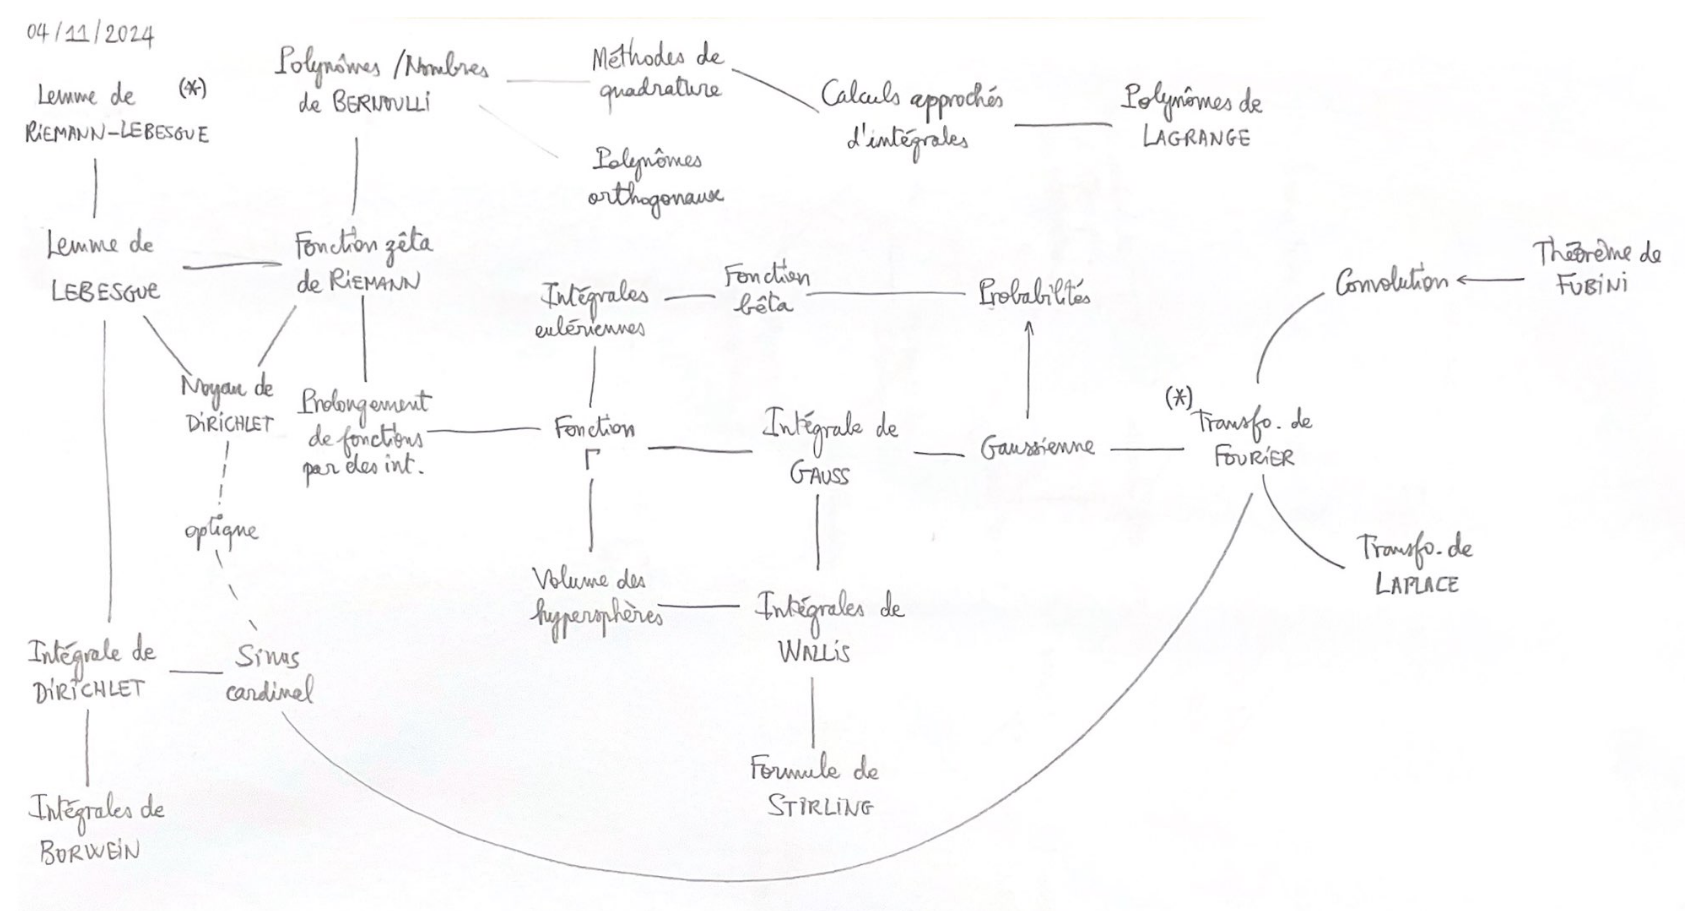
\includegraphics[width=1\linewidth]{chapitres/integration/documents/diagramme_integration.png}
    \caption{Ébauche d'un diagramme des chapitres}
\end{figure}

\todoinline{Chapitres validés : \\
01 : Changement de titre\\
02 : J'ai ajouté un encadré exercice à valider - Le titre de la figure, je le trouve bien - Les liens avec Bernoulli, ça me va mais garder l'encadrer pour rester self-contained.\\
03 : Relire Simpson - Dessins à compléter\\
04 : Peut être un dessin de plus\\
05 : validé \\
07 : Ajouter un graphique ?.\\
08 : Proposition de déplacement\\
09 : TF gaussienne : supprimé car intégré au 10\\
10 : Quelques citations à ajouter\\
11 : Quelques illustrations à terminer\\
12 : Presque validé. Illustrer les boules ?\\
13 : Presque validé après grosse modification pour bêta.\\
14 : Presque validé en supprimant le produit de convolution.\\
}

\todoinline{Créer une annexe avec les théorèmes utilisés ? Comme l'intégration par parties ? Ou alors on met juste un index des théorèmes et il n'y a ensuite qu'à aller chercher dans des livres... ou wikipedia...}

% 1ère version : OK
\section{Aire et fonction réciproque}

\begin{prop}
Soit $f$ de classe $\mathscr{C}^1$ sur $\interff{a}{b}$ telle que $f'$ soit strictement positive sur $\interff{a}{b}$. Alors,
\[
\int_{a}^{b} f(t) \d t + \int_{f(a)}^{f(b)} f^{-1}(t) \d t = b f(b) - a f(a).
\]
\end{prop}

\begin{elemsolution}
    \begin{enumerate}
    \item Comme $f' > 0$, alors $f$ est strictement croissante. Comme $f$ est continue, d'après le théorème de la bijection monotone, $f$ réalise une bijection de $\interff{a}{b}$ sur $\interff{f(a)}{f(b)}$.
    
    \item On utilise le changement de variable $\fonctionens[\phi]{\interff{a}{b}}{\interff{f(a)}{f(b)}},\, u \mapsto f(u)$. Alors, $\phi$ est de classe $\mathscr{C}^1$ et
    \begin{align*}
    \int_{f(a)}^{f(b)} f^{-1}(t) \d t
    &= \int_a^b f^{-1}\mathopen{}\big(f(u)\big) f'(u) \d u\\
    &= \int_a^b u f'(u) \d u\\
    &= \big[u f(u)\big]_a^b - \int_a^b f(u) \d u,
    \end{align*}
    où on a réalisé une intégration par parties.
    \end{enumerate}

    Finalement,
    \[
    \int_a^b f(t) \d t + \int_{f(a)}^{f(b)} f^{-1}(t) \d t = b f(b) - a f(a).
    \]
\end{elemsolution}

\begin{figure}[H]
    \centering
    \begin{tikzpicture}[line cap=round, >=latex]

\begin{scope}[local bounding box=struct, scale=1]

    \def\u{0.5}
    \def\v{0.2}

    \def\xa{5}
    \def\ya{0.5}
    \def\xb{6.5}
    \def\yb{1.5}
    \def\xc{8}
    \def\yc{4}

    \path (\xa, \ya)    coordinate (A)
        (\xb, \yb)    coordinate (B)
        (\xc, \yc)  coordinate (C)
        (\ya, \xa)    coordinate (A')
        (\yb, \xb)    coordinate (B')
        (\yc, \xc)  coordinate (C');

    \begin{scope}
        \clip (A') ..controls +(0.05*\u, 0.05*\u) and ( $(B') + (-5*\v, -0.5*\u)$ )..
        (B') ..controls +(5*\v, 0.5*\u) and ( $(C') + (-2*\v, -2*\v)$ )..
        (C') |- cycle;
        %\clip (A') ..controls +(0.05*\u, 0.05*\u) and ( $(B') + (-0.5*\v, -0.5*\u)$ )..
        %(B') ..controls +(5*\v, 0.5*\u) and ( $(C') + (-2*\v, -2*\v)$ )..
        %(C') |- cycle;
        \foreach \x in {\ya00, \ya01,...,\yc.000}   
            \draw[blue!15!white, opacity=0.5] (\x,0) -- ++(0,8);
    \end{scope}

    \fill[blue!15!white] (\ya,0) rectangle ++(\yc-\ya,\xa);

    \begin{scope}
        \clip (A) ..controls +(0.05*\u, 0.05*\u) and ( $(B) + (-0.5*\u, -5*\v)$ )..
        (B) ..controls +(0.5*\u, 5*\v) and ( $(C) + (-2*\v, -2*\v)$ )..
            (C) |- cycle;
        \foreach \x in {\xa.000, \xa.001,...,\xc.000}   
            \draw[red!15!white, opacity=0.5] (\x,-\ya) -- ++(0,10);
    \end{scope}

    \draw[thick, blue] 
        (A') ..controls +(0.05*\u, 0.05*\u) and ( $(B') + (-5*\v, -0.5*\u)$ )..
        (B') ..controls +(5*\v, 0.5*\u) and ( $(C') + (-2*\v, -2*\v)$ )..
        (C') node[right] {$\mathcal{C}_f^{-1}$};
        
    \draw[thick, red] 
        (A) ..controls +(0.05*\u, 0.05*\u) and ( $(B) + (-0.5*\u, -5*\v)$ )..
        (B) ..controls +(0.5*\u, 5*\v) and ( $(C) + (-2*\v, -2*\v)$ )..
            (C) node[above] {$\mathcal{C}_f$};


    \fill[red!15!white] (\xa,0) rectangle ++(\xc-\xa,\ya);

    \draw[gray] (-.5, -.5) -- (\xc + 0.5, \xc.5) node[below left] {\contour{white}{\footnotesize$y = x$}};

    \draw[dashed] (\xa, 0) node[black,below]{\footnotesize$a$} -- (A);
    \draw[dashed] (0, \ya) node[black,left]{\footnotesize$f(a)$} -- (A);
    
    \draw[dashed] (\xc, 0) node[black,below]{\footnotesize$b$} -- (C);
    \draw[dashed] (0, \yc) node[black,left]{\footnotesize$f(b)$} -- (C);

    \draw[dashed] (0, \xa) node[black,left]{\footnotesize$a$} -- (A');
    \draw[dashed] (\ya, 0) node[black,below]{\footnotesize$f(a)$} -- (A');
    
    \draw[dashed] (0, \xc) node[black,left]{\footnotesize$b$} -- (C');
    \draw[dashed] (\yc, 0) node[black,below]{\footnotesize$f(b)$} -- (C');

    \draw[->, black] (5.5,2) node[above] 
    {\footnotesize \contour{white}{$\displaystyle \int_a^b f(t)\, \mathrm{d} t$}} to [out=-90,in=180] ($(7,1.5)$);

    % \draw[->, black] (3,-0.5) node[below] 
    % {\footnotesize \contour{white}{$\displaystyle \int_{f(a)}^{f(b)} f^{-1}(t)\, \mathrm{d} t$}} to [out=70,in=-70] ($(3,1.5)$);
    \node at ((2.5, 5) {\footnotesize \contour{blue!15!white}{$\displaystyle \int_{f(a)}^{f(b)} f^{-1}(t)\, \mathrm{d} t$}};

    \draw[thick, ->] (-.5, 0) -- (\xc + 0.5, 0) node[above] {$x$};
    \draw[thick, ->] (0, -.5) -- (0, \xc + 0.5) node[left] {$y$};

\end{scope}

\end{tikzpicture}
    \caption{Illustration géométrique de la formule d'intégration par parties}
    \label{fig:i_01-une_propriete_geometrique_de_l_integrale}
\end{figure}

\begin{comment}
\begin{remarque}
La représentation graphique \ref{fig:i_01-une_propriete_geometrique_de_l_integrale} permet d'illustrer géométriquement la formule d'intégration par parties.

En effet, si $f$, $g$ sont de classe $\mathcal{C}^1$ et strictement monotones, alors elles sont bijectives. On a de plus \mbox{$\big(f \circ g^{-1}\big)^{-1} = g \circ f^{-1}$}. Ainsi, en appliquant la relation précédente à la fonction $f \circ g^{-1}$, on obtient
\begin{align*}
\int_{g(a)}^{g(b)} \big(f \circ g^{-1}\big)(u) \d u + \int_{(f\circ g^{-1})(g(a))}^{(f\circ g^{-1})(g(b))} \big(f \circ g^{-1}\big)^{-1}(u) \d u &= \begin{multlined}[t] 
g(b) \big(f \circ g^{-1}\big)\big(g(b)\big) \\
- g(a) \big(f \circ g^{-1}\big)\big(g(a)\big)
\end{multlined} \\
\int_{g(a)}^{g(b)} \big(f \circ g^{-1}\big)(u) \d u + \int_{f(a)}^{f(b)} \big(g \circ f^{-1}\big)(u) \d u
&= g(b) f(b) - g(a) f(a).
\end{align*}

Ainsi, en effectuant le changement de variable $t \mapsto g(t)$ (resp. $t \mapsto f(t)$) dans la première (resp. seconde) intégrale, on retrouve la formule d'intégration par parties :
\[
\int_a^b f(t) g'(t) \,\mathrm{d}t + \int_a^b g(t) f'(t) \,\mathrm{d}t = f(b) g(b) - f(a) g(a).
\]
\end{remarque}
\end{comment}

% TODO : insérer la partie application de Bernoulli
\section{Lemme de \textsc{Lebesgue}}

\todoinline{Parvenir à décommenter le marginnote suivant. D'après mes recherches sur internet, il faudrait "externaliser" la compilation des figures en pdflatex qui demandent trop de ressources.}

\begin{lemme}
% \marginnote[0cm]{Source : \cite{maths-france} Planche no 37. Intégration sur un segment}
Soit $a < b$.
\begin{enumerate}
\item On suppose que $f$ est une fonction de classe $\mathscr{C}^1$ sur $[a, b]$. Alors,
\[
\lim_{ \lambda \to +\infty} \int_a^b \sin(\lambda t) f(t) \d t = 0.
\]

\item Redémontrer le même résultat en supposant simplement que la fonction $f$ est continue par morceaux sur~$[a, b]$.
\end{enumerate}
\end{lemme}

\todoinline{
Ajout du graphique suivant, à supprimer ou améliorer en coloriant les aires positives et négatives ?
}

\todoarmand{Je suis partant pour laisser le graphique, j'ai ajouté une version avec les aires colorées.}

On constate sur la figure suivante que plus $\lambda$ est grand, plus les oscillations sont élevées et plus les aires comptées positivement et négativement se compensent.
\begin{center}
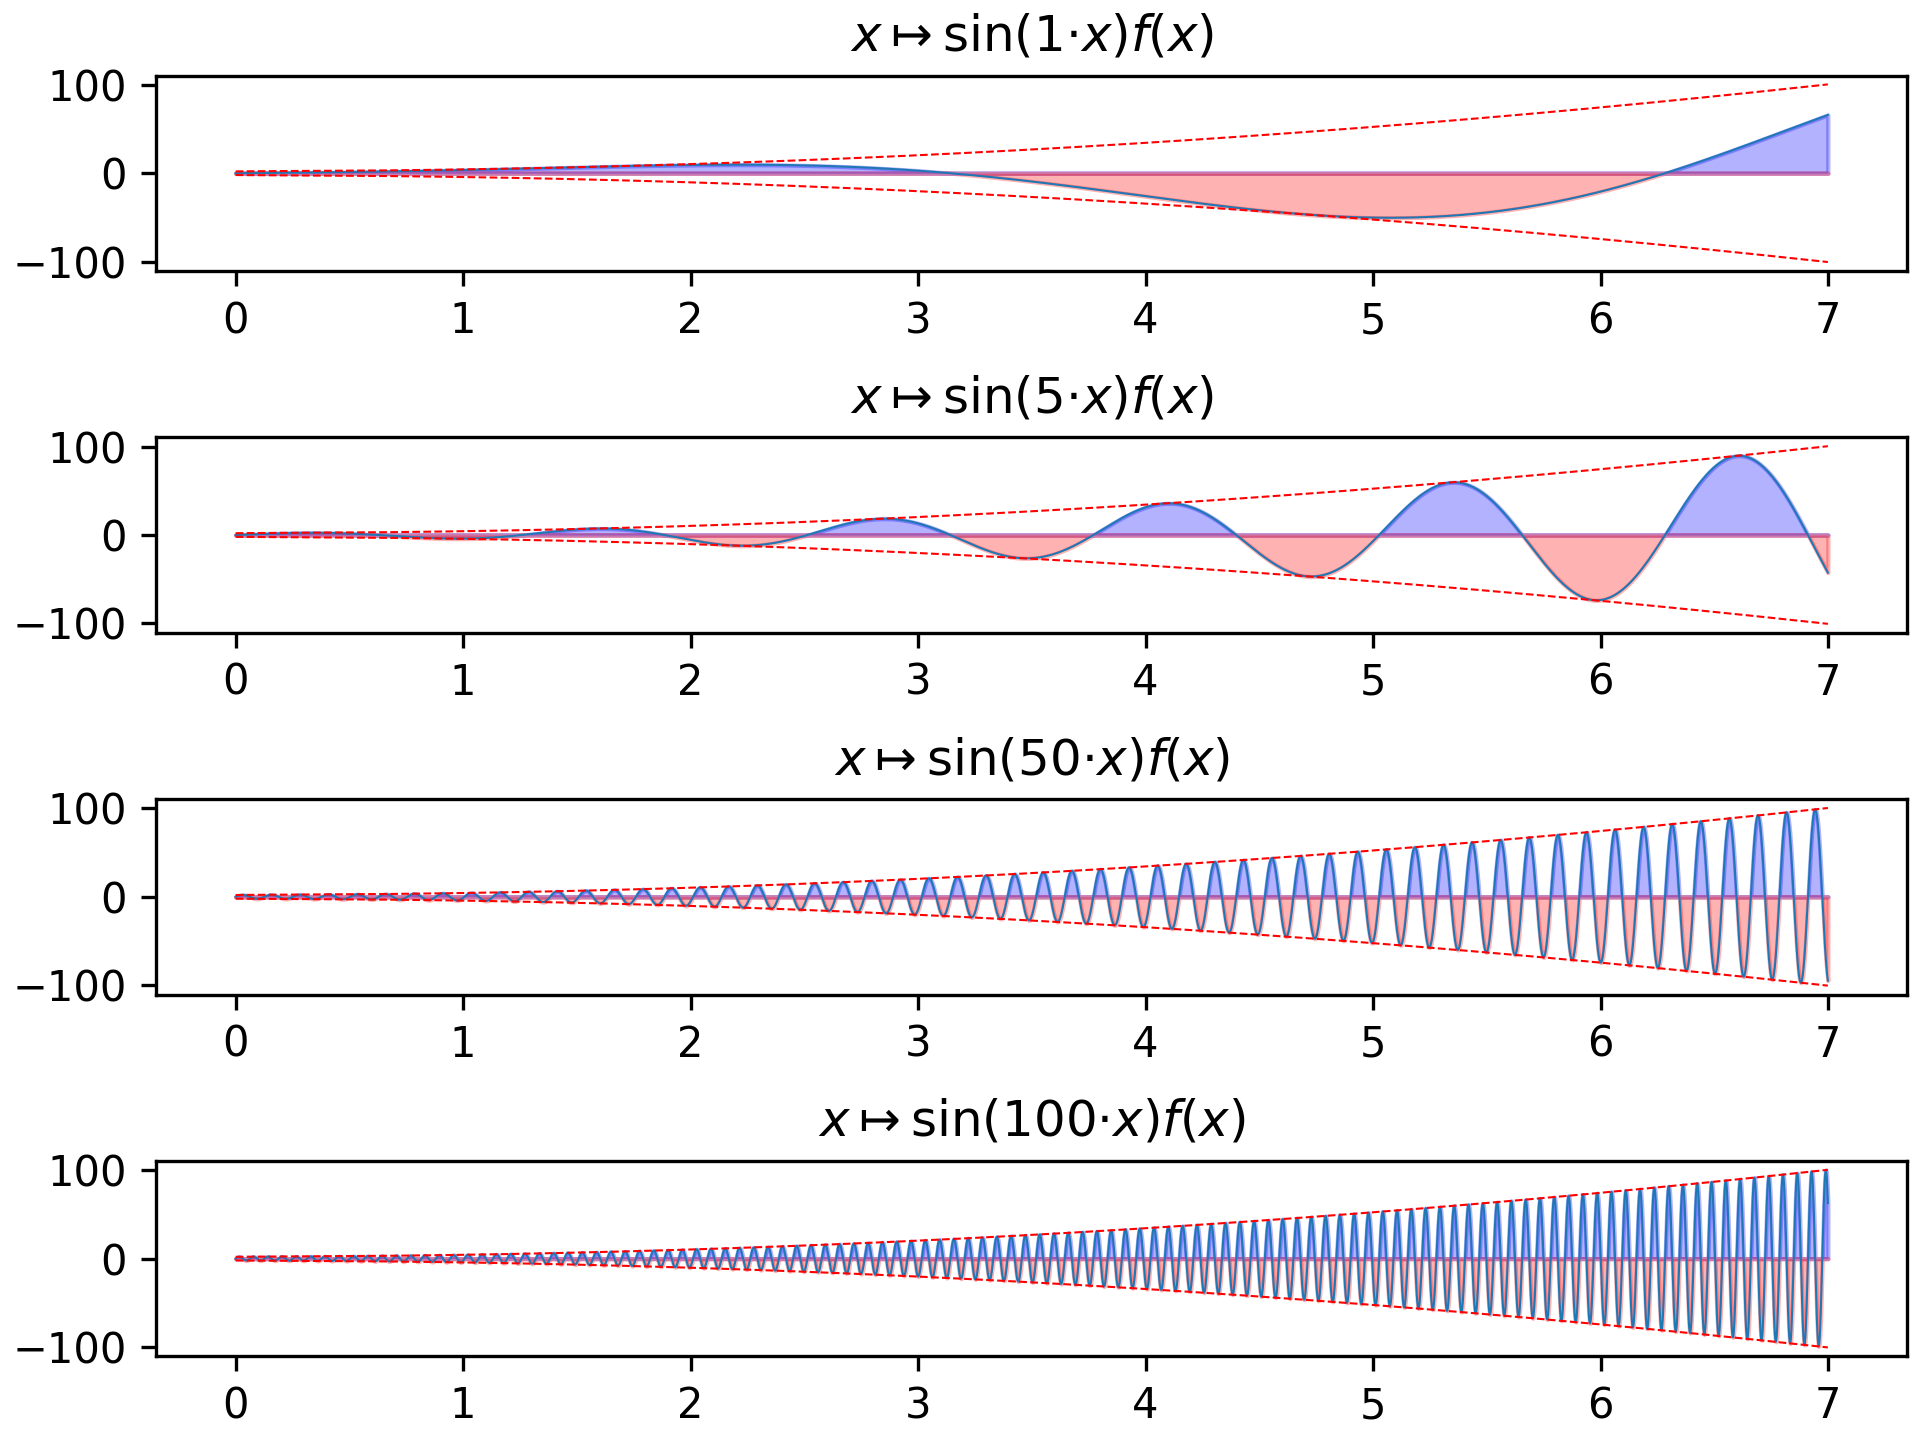
\includegraphics[width=0.75\textwidth]{illustrations/integration-02_lebesgue.png}
\end{center}

\begin{solution}
    \begin{enumerate}
        \item Puisque la fonction $f$ est de classe $\mathscr{C}^1$ sur $[a, b]$, on peut effectuer une intégration par parties qui fournit pour $\lambda > 0$:
        $$\left| \int_a^b f(t) \sin(\lambda t) \d t \right| = \left| \frac{1}{\lambda} \left( -\big[ \cos(\lambda t) f(t) \big]_a^b + \int_a^b f'(t) \cos(\lambda t) \d t  \right) \right| \leqslant \frac{1}{\lambda} \left( |f(a)| + |f(b)| + \int_a^b |f'(t)| \d t \right).$$
        Cette dernière expression tend vers $0$ quand $\lambda$ tend vers $+ \infty$, et donc $\int_a^b f(t) \sin(\lambda t) \d t$ tend vers $0$ quand $\lambda$ tend vers $+\infty$.
        \item Si la fonction $f$ est simplement supposée continue par morceaux, on ne peut donc plus effectuer une intégration par parties. \\
        Le résultat est clair si $f = 1$, car pour $\lambda > 0$, $\left| \int_a^b \sin(\lambda t) \d t \right| = \left| \frac{\cos(\lambda a) - \cos(\lambda b)}{\lambda} \right| \leqslant \frac{2}{\lambda}$. \\
        Le résultat s'étend aux fonctions constantes par linéarité de l'intégrale puis aux fonctions constantes par morceaux par additivité par rapport à l'intervalle d'intégration, c'est-à-dire aux fonctions en escaliers. Pour toute fonction $g$ continue par morceaux sur $[a, b]$, on note $\|g\|_{\infty} = \sup_{[a, b]} |g|$.\\
        Soit alors $f$ une fonction continue par morceaux sur $[a, b]$. \\
        \todoinline{Là on admet un théorème d'approximation non trivial et hors programme en PCSI. Il faut voir ce qu'on indique en introduction du chapitre ?}
        Soit $\varepsilon > 0$. Il existe une fonction en escalier $\varphi$ telle que $\|f - \varphi\|_\infty \leq \varepsilon$. De plus, d'après le point précédent, il existe un réel $\lambda_0$ strictement positif tel que pour tout $\lambda > \lambda_0$,
        \[
        \left|\int_a^b \sin(\lambda t) \varphi(t) \d t\right| \leq \varepsilon.
        \]
        Finalement, d'après l'inégalité triangulaire, pour tout $\lambda > \lambda_0$,
        \begin{align*}
        \left|\int_a^b f(t) \sin(\lambda t) \d t\right|
        &\leq         \left|\int_a^b (f(t) - \varphi(t)) \sin(\lambda t) \d t\right| + \left|\int_a^b \varphi(t) \sin(\lambda t) \d t\right|\\
        &\leq \norme{f - \varphi}_\infty (b - a) + \varepsilon\\
        &\leq \varepsilon (1 + b - a).
        \end{align*}
Finalement, $\lim\limits_{\lambda \to +\infty} \int_a^b f(t) \sin(\lambda t) \d t = 0$.
        \end{enumerate}
\end{solution}


% \todoinline{
% La variante proposée ci-dessous me semble difficile.
%
% Le calcul de $\sum \frac{1}{n^2}$ est classique et pourrait être directement généralisé avec St Cyr 1995 - Je mets une version dans le dossier /chapitres/integration/documents. En plus on ferait un peu de polynômes de Bernoulli.
%
% Le calcul de l'intégrale de Dirichlet est top.
% }

% \todoarmand{Cela me convient, nous pouvons supprimer la variante. On pourrait la remplacer par le  mais en renvoyant vers un exercice du chapitre polynômes.}

\bigskip


\todoinline{Ajouter des liens dans le texte ci-dessous.}

Nous allons utiliser le lemme de Lebesgue pour calculer certaines valeurs de la fonction $\zeta$ de Riemann. Nous verrons ultérieurement une autre utilisation au calcul de la valeur de l'intégrale de Dirichlet.

\todoinline{Partie re-rédigée, à relire !}

\todoinline{Citer sujet St Cyr 1995}

\todoinline{Faire référence à une section sur $\zeta$ et une section sur Bernoulli}

\todoinline{Dans la partie sur Bernoulli, il faudra :
la symétrie, la dérivée et les valeurs de $B_2(0)$ et $B_4(0)$}

On note $(B_n)$ la suite des polynômes de Bernoulli et, pour tout $x > 1$, $\zeta(x) = \sum\limits_{k=1}^{+\infty} \frac{1}{k^x}$.

\begin{theo}
Pour tout $m \geq 1$, $\zeta(2m) = (-1)^{m-1} (2 \pi)^{2m} \frac{B_{2m}(0)}{2}$.
\end{theo}

On rappelle que 
\begin{align*}
B_n(1 - x) &= (-1)^n B_n(x),\\
B_n'(x) &= n B_{n-1}(x).
\end{align*}

\begin{elem_sol}
Pour $k$ et $n$ entiers strictement positifs, on défnit:
\[
I_{n, k} = \int_0^1 B_n(t) \cos(2 k \pi t) \d t.
\]

\begin{enumerate}
\item Pour tout entier $p > 0$,
\[
I_{2p, k} = \frac{(-1)^{p-1}}{(2 k \pi)^{2p}} \quad \text{et} \quad I_{2p+1,k} = 0.
\]

En effet, en utilisant deux intégrations par parties successives,
\[
I_{n,k} = \frac{1}{4k^2 \pi^2} \big(B_{n-1}(1) - B_{n-1}(0) - I_{n-2, k} \big).
\]
De plus, $I_{0,k} = 0$, $I_{1,k} = 0$, $I_{2,k} = \frac{1}{4 \pi^2}$? Donc,
\[
\forall n \geqslant 3,\, I_{n,k} = - \frac{1}{4 k^2 \pi^2}I_{n-2, k}.
\]
On obtient ainsi le résultat annoncé
\end{enumerate}

Pour tout entier naturel $n$ strictement positif, on pose:
\[
\forall t \in \interoo{0}{1}, \quad \varphi_n(t) = \frac{B_n(t) - B_n(0)}{\sin(\pi t)}.
\]

\begin{enumerate}[resume]
\item Pour tout $n \geq 2$, la fonction $\varphi_n$ est prolongeable par continuité à $\interff{0}{1}$ et que le prolongement est de classe $\mathscr{C}^1$. En effet,

\begin{itemize}
\item D'après les quotients de fonctions de classe $\mathscr{C}^1$ dont le dénominateur ne s'annule pas, la fonction $\varphi_n$ est de classe $\mathscr{C}^1$ sur $\interoo{0}{1}$.

\item La fonction $B_n$ étant polynomiale, elle est de classe $\mathscr{C}^1$ en $0$ et, en utilisant la formule de \textsc{Taylor}--\textsc{Young},
\begin{align*}
\varphi_n(t) &= \frac{B'_n(0)t + \frac{B''_n(0)}{2}t^2 + o(t^2)}{\pi t \big(1 + o(t) \big)} \\
&= \frac{B'_n(0)}{\pi} + \frac{B''_n(0)}{2 \pi}t + o(t).
\end{align*}

Ainsi, $\lim\limits_0 \varphi_n = \frac{B'_n(0)}{\pi}$ et $\varphi_n$ est une fonction prolongeable par continuité en $0$.

\item
% De plus, $\lim\limits_{t \to 0} \frac{\varphi_n(t) - \frac{B'_n(0)}{\pi}}{t} = \frac{B''_n(0)}{2 \pi}$.
%
De plus, pour tout $t$ non nul, $\varphi'_n(t) = \frac{B'_n(t) \sin(\pi t) - \big(B_n(t) - B_n(0) \big) \pi \cos(\pi t)}{\sin(\pi t)^2}$. Ainsi, en effectuant un développement limité à l'ordre $2$ du numérateur, alors $\lim\limits_{t \to 0} \varphi'_n(t) = \frac{1}{2 \pi} B''_n(0)$.

D'après le théorème de prolongement des dérivées, $\varphi_n$ est prolongeable en une fonction de classe $\mathscr{C}^1$ sur $\interfo{0}{1}$.

Enfin, $\varphi_n(1-t) = (-1)^n \frac{B_n(t) - B_n(1)}{\sin(\pi t)}$. Comme, pour tout $n \geqslant 2$, $B_n(0) = B_n(1)$, alors la fonction $\varphi_n$ est bien prolongeable en une fonction de classe $\mathscr{C}^1$ sur $\interff{0}{1}$.
\end{itemize}
\end{enumerate}

Pour tout $N$ entier naturel non nul et $t \in \interoo{0}{1}$, on pose :
\[
D_n(t) = 1 + 2 \sum_{k=1}^N \cos(2k \pi t) = \frac{\sin\big((2N+1) \pi t \big)}{\sin(\pi t)}.
\]

\begin{enumerate}[resume]
\item Cette quantité, appelée noyau de Dirichlet, s'exprime simplement à l'aide de la fonction sinus :
\[
D_n(t) = \frac{\sin\big((2N+1) \pi t \big)}{\sin(\pi t)}.
\]
En effet, pour tout $t \in \interoo{0}{1}$, $\e^{2 \i k \pi t} \not= 1$. Ainsi, d'après la somme des termes d'une suite géométrique, 
    \begin{align*}
        \sum_{k=0}^N \e^{2 \i k \pi t} &= \frac{\e^{2 \i (N+1) \pi} - 1}{\e^{2 \i \pi} - 1} \\
        &= \e^{\i N \pi} \frac{\sin(N+1) \pi t}{\sin(\pi t)}. \\
        \sum_{k=0}^N \cos(2 k \pi t) &= \cos(N \pi t) \frac{\sin \big((N+1) \pi t \big)}{\sin(\pi t)}\text{, en prenant les parties réelles,} \\
        1 + 2 \sum_{k=1}^N \cos(2 k \pi t) &= 2 \frac{\cos(N \pi t) \sin \big((N+1) \pi t\big)}{\sin(\pi t)} - 1 \\
        &= \frac{\sin\big((2N+1) \pi t \big) + \sin( \pi t)}{\sin(\pi t)} - 1 \\
        &= \frac{\sin\big((2N+1) \pi t \big)}{\sin(\pi t)}.
    \end{align*}

\item Ainsi,
\[
\int_0^1 \varphi_{2m}(t) \sin \big((2N+1) \pi t \big) \d t
= - B_{2m}(0) + 2 \sum_{k=1}^N \frac{(-1)^{m-1}}{(2 k \pi)^{2m}}.
\]

En effet, d'après la définition de $\varphi_{2m}$,
\begin{align*}
\int_0^1 \varphi_{2m}(t) \sin \big((2N+1) \pi t \big) \d t &= \int_0^1 \big(B_{2m}(t) - B_{2m}(0) \big) \frac{\sin\big((2N+1) \pi t \big)}{\sin(\pi t)} \d t \\
&= \int_0^1 \big( B_{2m}(t) - B_{2m}(0) \big) \d t + \cdots \\
&\cdots + 2 \sum_{k=1}^N \int_0^1 \big(B_{2m}(t) - B_{2m}(0) \big) \cos(2 k \pi t) \d t \\
&= - B_{2m}(0) + 2 \sum_{k=1}^N \frac{(-1)^{m-1}}{(2 k \pi)^{2m}}.
\end{align*}

\item D'après le lemme de Lebesgue,
\[
\lim_{N\to+\infty} \int_0^1 \varphi_{2m}(t) \sin \big((2N+1) \pi t \big) \d t = 0
\]
et on obtient bien le résultat annoncé.
\end{enumerate}
\end{elem_sol}


\begin{remarque}
En utilisant les valeurs remarquables des premiers polynômes de Bernoulli, on obtient
\begin{align*}
\sum_{k=1}^{+\infty} \frac{1}{k^2} &= 2 \pi^2 B_2(0) = \frac{\pi^2}{6} \\
\sum_{k=1}^{+\infty} \frac{1}{k^4} &= -2^3 \pi^4 B_4(0) = \frac{\pi^4}{90}.
\end{align*}
\end{remarque}

% TODO : à choisir puis à compléter
\section{Calculs approchés d'intégrales}

Nous abordons dans cette section quelques méthodes dont le but est d’estimer la valeur numérique de l'intégrale d'une fonction donnée $f$ définie sur un domaine borné $\interff{a}{b}$:
\[
I = \int_a^b f(t) \d t.
\]
Ces méthodes nous fourniront une valeur approchée $\widetilde{I}$ de l'intégrale $I$ de sorte que \chevron{$\widetilde{I} \approx I$}. \\
Soient $a$ et $b$ deux réels tels que $a < b$. Pour tout entier naturel $p$ non nul, on note $(x_i)_{i\in\llbracket 0, p \rrbracket}$ la subdivision régulière de $[a, b]$ de pas $\frac{b-a}{p}$. Ainsi, pour tout $i \in \llbracket 0, p \rrbracket$,
\[
x_i = a + i\, \frac{b-a}{p}.
\]

\begin{defi}
Une méthode d'intégration est d'\emph{ordre} au moins $n$ si elle est exacte (\emph{i.e.} $\widetilde{I} = I$) pour les polynômes de degrés inférieurs ou égaux $n$ et non exacte pour au moins un polynôme de degré $n+1$.
\end{defi}

%-----------
\subsection{Méthode des rectangles à gauche}

La méthode des rectangles à gauche consiste, pour chacun des intervalles de la subdivision, à approcher l'aire sous la courbe représentative de $f$ par celle d'un rectangle dont la hauteur correspond à la valeur de $f$ sur la borne de gauche. Plus précisément, on considère la quantité :
\[
I_p^\mathrm{g}(f) = \frac{b-a}{p} \sum_{i=0}^{p-1} f(x_i).
\]

\begin{marginfigure}[-3cm]
    \centering
    %https://tex.stackexchange.com/questions/476702/riemann-sum-approaches-area-under-curve

\begin{tikzpicture}[scale=0.8,declare function={f(\x)=((1/3)*(\x)^(3)-3*(\x)^(2)+8*\x-3;}]
\coordinate (start) at (.8,{f(.8)});
\coordinate (x0) at (1,{f(1)});
\coordinate (x1) at (2,{f(2)});
\coordinate (x2) at (3,{f(3)});
\coordinate (x3) at (4,{f(4)});
\coordinate (x4) at (5,{f(5)});
\coordinate (end) at (5.05,{f(5.05)});
\draw[fill=teal!20!white] (1,0) rectangle (2,{f(1)});
\draw[fill=teal!20!white] (2,0) rectangle (3,{f(2)});
\draw[fill=teal!20!white] (3,0) rectangle (4,{f(3)});
\draw[fill=teal!20!white] (4,0) rectangle (5,{f(4)});
%\draw (5,0)--(5,{f(5)});
\draw [-latex] (-0.5,0) -- (6,0) node (xaxis) [below] {$x$};
\draw [-latex] (0,-0.5) -- (0,5) node [left] {$f(x)$};
\foreach \x/\xtext in {1/a=x_0 ,2/x_1, 3/x_2 , 4/x_3 , 5/b=x_4}
 \draw[xshift=\x cm] node[below=2pt,fill=white,font=\small, anchor=south, yshift=-5mm] {$\xtext$};
\draw[domain=.5:5.3,samples=200,variable=\x,blue,thick] plot ({\x},{f(\x)});                 
\foreach \n in {0,1,2,3}
\draw[blue,fill=blue] (x\n) circle (2pt) node[font=\normalsize] {$ $};    
\draw[latex-latex] (2,1)--(3,1) node[midway, anchor=south] {$\frac{b-a}{p}$};      
\end{tikzpicture}
    \caption{Illustration de la méthode des rectangles à gauche}
\end{marginfigure}
\marginnote[3cm]{Animation de la méthode des rectangles à gauche : \url{https://acamanes.github.io/psi/psi_doc/animations/integration_segment/01-methode_des_rectangles_a_gauche.mp4}}

\begin{prop}
La méthode des rectangles à gauche est d'ordre $0$. De plus, si $f$ est de classe $\mathscr{C}^1$, l'erreur commise est en $O(1/p)$.
\end{prop}

\begin{exercice}
Soit $f$ une fonction de classe $\mathscr{C}^1$ sur le segment $\interff{a}{b}$. On note $F$ une primitive de $f$ et $M_1 = \sup_{\interff{a}{b}} \module{f'}$.
\begin{questions}
\item Montrer que
\[
\forall i \in \interent{0}{p-1},\quad 
\module{F(x_{i+1}) - F(x_i) - (x_{i+1} - x_i) F'(x_i)} \leqslant \frac{M_1}{2} (x_{i+1}-x_i)^2.
\]

\item En déduire que
\[
\module{\int_{\interff{a}{b}} f(t) \d t - I_p^\mathrm{g}(f)}
\leqslant \frac{M_1 (b-a)^2}{2 p}.
\]

\item Utiliser la méthode des rectangles à gauche pour calculer une valeur approchée de l'intégrale de la fonction $x \mapsto x - a$.

\item Conclure.
\end{questions}
\end{exercice}

\begin{elemsolution}

\begin{reponses}
\item Il s'agit d'une application de la formule de \textsc{Taylor} avec reste intégal.

\item En utilisant la relation de \textsc{Chasles},
\begin{align*}
\module{\int_{\interff{a}{b}} f(t) \d t - I_p^\mathrm{g}(f)}
&\leqslant \sum_{i=1}^{p-1} \module{\int_{\interff{x_i}{x_{i+1}}} f(x) \d x - (x_{i+1} - x_i) f(x_i)}\\
&\leqslant \sum_{i=1}^{p-1} \frac{M_1}{2} (x_{i+1} - x_i)^2
% &\leq \frac{M_1}{2} (b - a) \sum_{i=1}^{p-1} (x_{i+1} - x_i)\\
\leqslant \frac{M_1 (b-a)^2}{2 p}.
\end{align*}

\item On remarque que, dans ce cas, $M_1 = b - a$ et la borne est atteinte.

\item La méthode des rectangles à gauche est exacte si $f$ est constante. Cependant, le calcul précédent montre que si $\fonctionligne[f]{x}{x - a}$, alors la méthode ne donne pas la valeur exacte de l'intégrale. La méthode est donc d'ordre $0$.
\end{reponses}
\end{elemsolution}

%-----------
\subsection{Méthode des rectangles médians}

La méthode des rectangles médians consiste, pour chacun des intervalles de la subdivision, à approcher l'aire sous la courbe représentative de $f$ par celle d'un rectangle dont la hauteur correspond à la valeur de $f$ au milieu de la subdivision. Plus précisément, on considère la quantité :
\[
I_p^\mathrm{m}(f) = \frac{b-a}{p} \sum_{i=0}^{p-1} f\left(\frac{x_i + x_{i+1}}{2} \right).
\]

\begin{prop}
La méthode des rectangles médians est d'ordre $1$. De plus, si $f$ est de classe $\mathscr{C}^2$, l'erreur commise est en $O(1/p^2)$.
\end{prop}

\begin{marginfigure}[-3cm]
    \centering
    \begin{tikzpicture}[scale=0.8,declare function={f(\x)=((1/3)*(\x)^(3)-3*(\x)^(2)+8*\x-3;}]
\coordinate (start) at (.8,{f(.8)});
\coordinate (x0) at (1.5,{f(1.5)});
\coordinate (x1) at (2.5,{f(2.5)});
\coordinate (x2) at (3.5,{f(3.5)});
\coordinate (x3) at (4.5,{f(4.5)});
\coordinate (x4) at (5.5,{f(5.5)});
\coordinate (end) at (5.05,{f(5.05)});
\draw[fill=teal!20!white] (1,0) rectangle (2,{f(1.5)});
\draw[fill=teal!20!white] (2,0) rectangle (3,{f(2.5)});
\draw[fill=teal!20!white] (3,0) rectangle (4,{f(3.5)});
\draw[fill=teal!20!white] (4,0) rectangle (5,{f(4.5)});

\draw[dashed] (1.5, 0) -- (1.5,{f(1.5)});
\draw[dashed] (2.5, 0) -- (2.5,{f(2.5)});
\draw[dashed] (3.5, 0) -- (3.5,{f(3.5)});
\draw[dashed] (4.5, 0) -- (4.5,{f(4.5)});

\draw [-latex] (-0.5,0) -- (6,0) node (xaxis) [below] {$x$};
\draw [-latex] (0,-0.5) -- (0,5) node [left] {$f(x)$};
\foreach \x/\xtext in {1/a=x_0 ,2/x_1, 3/x_2 , 4/x_3 , 5/b=x_4}
 \draw[xshift=\x cm] node[below=2pt,fill=white,font=\small, anchor=south, yshift=-5mm] {$\xtext$};
\draw[domain=.5:5.3,samples=200,variable=\x,blue,thick] plot ({\x},{f(\x)});                 
\foreach \n in {0,1,2,3}
\draw[blue,fill=blue] (x\n) circle (2pt) node[font=\normalsize] {$ $};    
% \draw[latex-latex] (2,1)--(3,1) node[midway, anchor=south] {$\frac{b-a}{p}$};      
\end{tikzpicture}
    \caption{Illustration de la méthode des rectangles médians}
\end{marginfigure}
\marginnote[3cm]{Animation de la méthode des rectangles médians : \url{https://acamanes.github.io/psi/psi_doc/animations/integration_segment/02-methode_des_rectangles_medians.mp4}}

\begin{exercice}
Soit $f$ une fonction de classe $\mathscr{C}^2$ sur le segment $\interff{a}{b}$. On note $F$ une primitive de $f$ et $M_2 = \sup_{\interff{a}{b}} \module{f''}$. Pour tout entier $i \in \interent{0}{p-1}$, on pose $\gamma_i = \frac{x_i + x_{i+1}}{2}$ le milieu du segment $\interff{x_i}{x_{i+1}}$.
\begin{questions}
\item Montrer que
\[
\forall i \in \interent{0}{p-1},\quad 
(x_{i+1} - x_i) f(\gamma_i) = \int_{x_i}^{x_{i+1}} \left(f(\gamma_i) + (t - \gamma_i) f'(\gamma_i) \right) \d t.
\]    

\item Montrer que
\[
\forall i \in \interent{0}{p-1},\quad 
\module{F(x_{i+1}) - F(x_i) - (x_{i+1} - x_i) F'(\gamma_i)} \leqslant \frac{M_2}{24} (x_{i+1} - x_i)^3.
\]

\item En déduire que
\[
\module{\int_{[a,b]} f(t) \d t- I_p^\mathrm{m}(f)} \leqslant \frac{M_2 (b-a)^3}{24 p^2}.
\]

\item Appliquer l'inégalité précédente à la fonction $x \mapsto (x - a)^2$.

\item Conclure.
\end{questions}
\end{exercice}


\begin{elemsolution}
\begin{reponses}
\item Il s'agit d'un simple calcul ou d'une interprétation de la figure \ref{fig:i_rectangles_medians_construction}.

\item Ainsi, d'après la formule de \textsc{Taylor} avec reste intégral,
\begin{align*}
\module{F(x_{i+1}) - F(x_i) - (x_{i+1} - x_i) F'(\gamma_i)}
&= \module{\int_{x_i}^{x_{i+1}} \left(f(t) - f(\gamma_i) - (t - \gamma_i) f'(\gamma_i)\right) \d t}
\leqslant \frac{M_2}{24} (x_{i+1} - x_i)^3.
\end{align*}

\begin{marginfigure}[0cm]
    \centering
    \begin{tikzpicture}[scale=0.8,declare function={f(\x)=((1/3)*(\x)^(3)-3*(\x)^(2)+8*\x-3;}, declare function={g(\x)=-\x+6;},]
\coordinate (xm) at (3,{f(3)});

\draw[fill=teal!20!white] (2,0) rectangle (4,{f(3)});
\fill[red, opacity=0.2,ultra thick] (2,0) -- (2,{g(2)}) -- (4, {g(4)}) -- (4, 0);

\draw[dashed] (3, 0) -- (3,{f(3)});
\draw[dashed] (2, {f(3)}) -- (2,{g(2)});

\draw [-latex] (-0.5,0) -- (6,0) node (xaxis) [below] {$t$};
\draw [-latex] (0,-0.5) -- (0,5);
% \foreach \x/\xtext in {1/a=x_0 ,2/x_1, 3/x_2 , 4/x_3 , 5/b=x_4}
\draw[xshift=2 cm] node[below=2pt,fill=white,font=\small, anchor=south, yshift=-5mm] {$x_i$};
\draw[xshift=3 cm] node[below=2pt,fill=white,font=\small, anchor=south, yshift=-5mm] {$\gamma_i$};
\draw[xshift=4 cm] node[below=2pt,fill=white,font=\small, anchor=south, yshift=-5mm] {$x_{i+1}$};
\draw[domain=.5:5.3,samples=200,variable=\x,blue,thick] plot ({\x},{f(\x)}) node[right] {$f(t)$};  
\draw[domain=1.5:4.5,samples=200,variable=\x,red,thick] plot ({\x},{g(\x)}) node[right] {$f(\gamma_i) + (t - \gamma_i) f'(\gamma_i)$}; 
% \foreach \n in {0,1,2,3}
\draw[blue,fill=blue] (xm) circle (2pt) node[font=\normalsize] {$ $};    
% \draw[latex-latex] (2,1)--(3,1) node[midway, anchor=south] {$\frac{b-a}{p}$};      
\end{tikzpicture}
    \caption{}
    \label{fig:i_rectangles_medians_construction}
\end{marginfigure}

\item Comme pour la méthode des rectangles à gauche, il s'agit d'une application de la formule de \textsc{Chasles}.

\item On montre que la borne est atteinte pour $f : x \mapsto (x - a)^2$.

\item La méthode des rectangles médians est exacte si $f$ est un polynôme de degré $1$. Cependant, si $f$ est la fonction $x \mapsto (x - a)^2$, le calcul précédent montre que la méthode des rectangles médians ne donne pas la valeur exacte de l'intégrale. La méthode est donc d'ordre $1$.
\end{reponses}
\end{elemsolution}

%-----------
\subsection{Méthode des trapèzes}

La méthode des trapèzes consiste, pour chacun des intervalles de la subdivision, à approcher l'aire sous la courbe représentative de $f$ par celle d'un trapèze. Plus précisément, on considère la quantité :
\[
I_p^\mathrm{t}(f) =  \frac{b-a}{p} \sum_{i=0}^{p-1} \frac{f(x_i) + f(x_{i+1})}{2}.
\]

\begin{marginfigure}[0cm]
    \centering
    \begin{tikzpicture}[scale=0.8,declare function={f(\x)=((1/3)*(\x)^(3)-3*(\x)^(2)+8*\x-3;}]
\coordinate (start) at (.8,{f(.8)});
\coordinate (x0) at (1,{f(1)});
\coordinate (x1) at (2,{f(2)});
\coordinate (x2) at (3,{f(3)});
\coordinate (x3) at (4,{f(4)});
\coordinate (x4) at (5,{f(5)});
\coordinate (end) at (5.05,{f(5.05)});

\draw[fill=teal!20!white] (1,0)--(1,{f(1)})--(2,{f(2)})--(2,0);
\draw[fill=teal!20!white] (2,0)--(2,{f(2)})--(3,{f(3)})--(3,0);
\draw[fill=teal!20!white] (3,0)--(3,{f(3)})--(4,{f(4)})--(4,0);
\draw[fill=teal!20!white] (4,0)--(4,{f(4)})--(5,{f(5)})--(5,0);


%\draw (5,0)--(5,{f(5)});
\draw [-latex] (-0.5,0) -- (6,0) node (xaxis) [below] {$x$};
\draw [-latex] (0,-0.5) -- (0,5) node [left] {$f(x)$};
\foreach \x/\xtext in {1/a=x_0 ,2/x_1, 3/x_2 , 4/x_3 , 5/b=x_4}
 \draw[xshift=\x cm] node[below=2pt,fill=white,font=\small, anchor=south, yshift=-5mm] {$\xtext$};
\draw[domain=.5:5.3,samples=200,variable=\x,blue,thick] plot ({\x},{f(\x)});                 
\foreach \n in {0,1,2,3,4}
\draw[blue,fill=blue] (x\n) circle (2pt) node[font=\normalsize] {$ $};    
% \draw[latex-latex] (2,1)--(3,1) node[midway, anchor=south] {$\frac{b-a}{p}$};      
\end{tikzpicture}
    \caption{Illustration de la méthode des trapèzes}
\end{marginfigure}
\marginnote[6cm]{Animation de la méthode des trapèzes : \url{https://acamanes.github.io/psi/psi_doc/animations/integration_segment/03-methode_des_trapezes.mp4}}

\begin{prop}
La méthode des trapèzes est d'ordre $1$. De plus, si $f$ est de classe $\mathscr{C}^2$, l'erreur commise est en $O(1/p^2)$.
\end{prop}

\begin{exercice}
Soit $f$ une fonction de classe $\mathscr{C}^2$. On note $M_2 = \sup_{[a,b]} \module{f''}$. Pour tout $i \in \interent{0}{p-1}$, on note $\phi_i$ l'approximation affine sur $\interff{x_i}{x_{i+1}}$ de $f$ et $g_i = f - \phi_i$.
\begin{questions}
\item Montrer que
\[
\forall i \in \interent{0}{p-1},\quad 
\int_{x_i}^{x_{i+1}} f''(t)\,(t - x_i) (x_{i+1} - t) \d t = - 2 \int_{x_i}^{x_{i+1}} g_i(t) \d t.
\]

\item Montrer que
\[
\forall i \in \interent{0}{p-1},\quad 
\module{\int_{x_i}^{x_{i+1}} f(t) \d t - I_p^\mathrm{t}(f)}
\leqslant \frac{M_2}{2} \cdot \frac{(b - a)^3}{6}.
\]

\item En déduire que
\[
\module{\int_{[a,b]} f(t) \d t - I_p^\mathrm{t}(f)} \leqslant \frac{M_2 (b-a)^3}{12 p^2}.
\]

\item Appliquer l'égalité précédente à la fonction $x \mapsto (x - a)^2$.

\item Conclure.
\end{questions}
\end{exercice}

\begin{elemsolution}
\begin{reponses}
\item Il suffit d'effectuer deux intégrations par parties successives.

\item D'après la relation précédente, on établit que
\begin{align*}
\module{\int_{x_i}^{x_{i+1}} f(t) \d t - I_p^\mathrm{t}(f)}
&\leqslant \int_{x_i}^{x_{i+1}} \module{f(t) - \phi_i(t)} \d t\\
&\leqslant \frac{M_2}{2} \int_{x_i}^{x_{i+1}} (t - x_i) (x_{i+1} - t) \d t
\leqslant \frac{M_2}{2} \cdot \frac{(b - a)^3}{6}.
\end{align*}

\item Comme pour les méthodes précédentes, on utilise la relation de \textsc{Chasles}.

\item On montre que cette borne est atteinte pour $f : x \mapsto (x - a)^2$.

\item La méthode des trapèzes est exacte si $f$ est un polynôme de degré $1$. Cependant, si $f$ est la fonction $x \mapsto (x - a)^2$, le calcul précédent montre qur la méthode des trapèzes ne donne pas la valeur exacte de l'intégrale. La méthode est donc d'ordre $2$.
\end{reponses}
\end{elemsolution}

\begin{marginfigure}[-1cm]
\begin{subfigure}{.5\textwidth}
    \centering
\begin{tikzpicture}[scale=0.6]

\pgfmathdeclarefunction{f}{1}{%
    \pgfmathparse{((#1 - 3) / 1.5)^2 + 1}%
}
% ,declare function={f(\x)=((\x-3)/1.5)^2+1;}]
\coordinate (start) at (.8,{f(.8)});
\coordinate (x0) at (1,{f(1)});
\coordinate (x1) at (1+4/3,{f(1+4/3)});
\coordinate (x2) at (1+8/3,{f(1+8/3)});
\coordinate (x3) at (1+12/3,{f(1+12/3)});
\coordinate (end) at (5.05,{f(5.05)});

\draw[fill=teal!20!white] (1,0)--(1,{f(1)})--(1+4/3,{f(1+4/3)})--(1+4/3,0);
\draw[fill=teal!20!white] (1+4/3,0)--(1+4/3,{f(1+4/3)})--(1+8/3,{f(1+8/3)})--(1+8/3,0);
\draw[fill=teal!20!white] (1+8/3,0)--(1+8/3,{f(1+8/3)})--(5,{f(5)})--(5,0);

\draw[domain=.5:5.3,samples=200,variable=\x,blue,thick] plot ({\x},{f(\x)});                 

\draw[blue,fill=blue] (x0) circle (2pt);    
\draw[blue,fill=blue] (x1) circle (2pt);    
\draw[blue,fill=blue] (x2) circle (2pt);    
\draw[blue,fill=blue] (x3) circle (2pt);    

\end{tikzpicture}
    \caption{Cas convexe}
\end{subfigure}%
\begin{subfigure}{.5\textwidth}
    \centering
\begin{tikzpicture}[scale=0.6
% ,declare function={f(\x)=-((\x-3)/1.5)^2+3.5;}
]

\pgfmathdeclarefunction{f}{1}{%
    \pgfmathparse{-((#1 - 3) / 1.5)^2 + 3.5}%
}
\coordinate (start) at (.8,{f(.8)});
\coordinate (x0) at (1,{f(1)});
\coordinate (x1) at (1+4/3,{f(1+4/3)});
\coordinate (x2) at (1+8/3,{f(1+8/3)});
\coordinate (x3) at (1+12/3,{f(1+12/3)});
\coordinate (end) at (5.05,{f(5.05)});

\draw[fill=teal!20!white] (1,0)--(1,{f(1)})--(1+4/3,{f(1+4/3)})--(1+4/3,0);
\draw[fill=teal!20!white] (1+4/3,0)--(1+4/3,{f(1+4/3)})--(1+8/3,{f(1+8/3)})--(1+8/3,0);
\draw[fill=teal!20!white] (1+8/3,0)--(1+8/3,{f(1+8/3)})--(5,{f(5)})--(5,0);

\draw[domain=.5:5.3,samples=200,variable=\x,blue,thick] plot ({\x},{f(\x)});                 

\draw[blue,fill=blue] (x0) circle (2pt);    
\draw[blue,fill=blue] (x1) circle (2pt);    
\draw[blue,fill=blue] (x2) circle (2pt);    
\draw[blue,fill=blue] (x3) circle (2pt);  

\end{tikzpicture}
    \caption{Cas concave}
\end{subfigure}
\caption{Illustration de la remarque \ref{remarquemethodetrapezes}}
\end{marginfigure}

\begin{remarque}\label{remarquemethodetrapezes}
Lorsque $f$ est de classe $\mathscr{C}^2$ et convexe (resp. concave), alors $f'' \geqslant 0$ (resp. $\leqslant 0$) et, pour tout $p$ entier naturel, \mbox{$\int_{[a,b]} f \leqslant I_p^\mathrm{t}(f)$} (resp. \mbox{$\int_{[a,b]} f \geqslant I_p^\mathrm{t}(f)$}). On obtient ainsi une valeur approchée par excès (resp. par défaut) de l'intégrale.
\end{remarque}

\subsection{Méthode de \textsc{Simpson}}

La méthode de \textsc{Simpson} consiste, pour chacun des intervalles de la subdivision, à approcher la fonction $f$ par un polynôme de degré inférieur ou égal à $2$. Plus précisément, on considère la quantité :
\[
I_p^\mathrm{s}(f) = \frac{b-a}{6 p} \sum_{i=0}^{p-1} \left[f(x_i)+ 4 f\left(\frac{x_i + x_{i+1}}{2}\right) + f(x_{i+1})\right].
\]

\begin{prop}
Dans la méthode de \textsc{Simpson}, si $f$ est de classe $\mathscr{C}^4$, l'erreur commise est en $O(1/p^4)$.
\end{prop}

\todoinline{Tu aurais le courage de vérifier le calcul suivant ?}

\begin{exercice}
Soit $f$ une fonction de classe $\mathscr{C}^4$ sur le segment $[a, b]$. On pose $M_4 = \sup_{[a,b]} \big\vert f^{(4)} \big\vert$.

Pour tout $i \in \interent{0}{p-1}$, notons $\gamma_i = \frac{x_i + x_{i+1}}{2}$ le milieu de la subdivision et $h_i = \frac{x_{i+1} - x_i}{2}$ la moitié de sa longueur.
\begin{questions}
\item Montrer que pour tout $i \in \interent{0}{p-1}$,
\[
F(x_{i+1}) - F(x_i)
= \begin{multlined}[t] 
2 h_i f(\gamma_i) + \frac{h_i{}^3}{3} f''(\gamma_i) \\
+ \frac{h_i{}^5}{24} \int_0^1 (1 - t)^4 \left[f^{(4)}(\gamma_i + t h_i) + f^{(4)}(\gamma_i - t h_i)\right] \d t.
\end{multlined} 
\]

\item Montrer que pour tout $i \in \interent{0}{p-1}$,
\[
\module{f(x_{i+1}) + f(x_i) - 2 f(\gamma_i) - h_i{}^2 f(\gamma_i)} \leqslant \frac{h_i{}^4 \times 2 M_4}{4!}.
\]

\item En déduire que pour tout $i \in \interent{0}{p-1}$,
\[
\module{\int_{x_i}^{x_{i+1}} f(t) \d t - \frac{h_i}{3} \left[f(x_i) + 4 f(\gamma_i) + f(x_{i+1})\right]}
\leqslant \frac{(x_{i+1} - x_i)^5}{720}.
\]

\item Conclure.
\end{questions}
\end{exercice}

\begin{elemsolution}
\begin{reponses}
\item D'après la formule de \textsc{Taylor} avec reste intégral appliquée à une primitive $F$ de $f$,
\begin{align*}
F(\gamma_i + h_i)
&= \begin{aligned}[t]F(\gamma_i) + h_i f(\gamma_i) + \frac{h_i{}^2}{2} f'(\gamma_i) + \frac{h_i{}^3}{6} f''(\gamma_i) + \frac{h_i{}^4}{24} f'''(\gamma_i) \\ + \frac{h_i{}^5}{24} \int_0^1 (1 - t)^4 f^{(4)}(\gamma_i + t h_i) \d t,\\
\end{aligned} \\
\intertext{et}
F(\gamma_i - h_i)
&= \begin{aligned}[t]F(\gamma_i) - h_i f(\gamma_i) + \frac{h_i{}^2}{2} f'(\gamma_i) - \frac{h_i{}^3}{6} f''(\gamma_i) + \frac{h_i{}^4}{24} f'''(\gamma_i) \\ - \frac{h_i{}^5}{24} \int_0^1 (1 - t)^4 f^{(4)}(\gamma_i - t h_i) \d t.
\end{aligned}
\end{align*}

Comme $\gamma_i - h_i = x_i$ et $\gamma_i + h_i = x_{i+1}$, le résultat s'obtient en soustrayant les deux relations précédentes.


\item On applique la formule de \textsc{Taylor} avec reste intégral à la fonction $f$ sur $[\gamma_i - h_i, \gamma_i]$ et $[\gamma_i, \gamma_i + h_i]$.

\item Finalement,
\begin{align*}
\module{\int_{x_i}^{x_{i+1}} f(t) \d t - \frac{h_i}{3} \left[f(x_i) + 4 f(\gamma_i) + f(x_{i+1})\right]}
&\leqslant \module{\frac{h_i}{3} \left[f(x_i) - 2 f(\gamma_i) + f(x_{i+1}) - h_i{}^2 f''(\gamma_i)\right]} + \frac{h_i{}^5 2 M_4}{5! p^5}\\
&\leqslant h_i{}^5 \left[\frac{2}{3 \times 4!} + \frac{2}{5!}\right]\\
&\leqslant \frac{2 h_i{}^5}{45}
\leqslant \frac{(x_{i+1} - x_i)^5}{720}.
\end{align*}

\item On conclut à l'aide de la relation de \textsc{Chasles} :
\[
\module{\int_a^b f(t) \d t - I_p^\mathrm{s}(f)} \leq \frac{M_4 (b-a)^5}{720 p^4}.
\]
% \[
% \module{I_p^s(f) - \int_a^b f(t) \d t} \leq \frac{M_4 (b-a)^5}{2880 p^4}.
% \]
\end{reponses}
\end{elemsolution}

\begin{figure}[H]
    \centering
    \newcommand*{\parabolaShading}[6]{
\fill [cyan!10, domain=(#1:#5), variable=\x] (#1,0)  -- plot 
    (  {\x},{(#2*(\x-#3)*(\x-#5)/((#1-#3)*(#1-#5)))+
            (#4*(\x-#1)*(\x-#5)/((#3-#1)*(#3-#5)))+
            (#6*(\x-#1)*(\x-#3)/((#5-#1)*(#5-#3)))} )
    -- (#5,0) -- cycle;
}
\newcommand*{\parabolaLines}[6]{
\draw plot [domain=(#1-0.25):(#5+0.25)] %can be adjusted
    (   {\x},{(#2*(\x-#3)*(\x-#5)/((#1-#3)*(#1-#5)))+
            (#4*(\x-#1)*(\x-#5)/((#3-#1)*(#3-#5)))+
            (#6*(\x-#1)*(\x-#3)/((#5-#1)*(#5-#3)))} );
}
\newcommand*{\shadeWithBoundedDomainAndColor}[9]{ %first 6 are points; 7,8 are domain; 9 is color
\fill [#9, domain=(#7:#8), variable=\x] (#7,0)  -- plot 
    (  {\x},{(#2*(\x-#3)*(\x-#5)/((#1-#3)*(#1-#5)))+
            (#4*(\x-#1)*(\x-#5)/((#3-#1)*(#3-#5)))+
            (#6*(\x-#1)*(\x-#3)/((#5-#1)*(#5-#3)))} )
    -- (#8,0) -- cycle;
}

\begin{tikzpicture}
\coordinate (p1) at (0.7,3);
\coordinate (p2) at (1,3.3);
\coordinate (p3) at (2,2.5);
\coordinate (p4) at (3,2.5);
\coordinate (p5) at (4,3.5);
\coordinate (p6) at (5,4.1);
\coordinate (p7) at (6,3.4);
\coordinate (p8) at (7,4.1);
\coordinate (p9) at (8,4.6);
\coordinate (p10) at (9,4);
\coordinate (p11) at (9.5,4.7);

%Shading
\parabolaShading{1}{3.3}{2}{2.5}{3}{2.5}
%\parabolaShading{2}{2.5}{3}{2.5}{4}{3.5}
\parabolaShading{3}{2.5}{4}{3.5}{5}{4.1}
%\parabolaShading{4}{3.5}{5}{4.1}{6}{3.4}
\parabolaShading{5}{4.1}{6}{3.4}{7}{4.1}
%\parabolaShading{6}{3.4}{7}{4.1}{8}{4.6}
\parabolaShading{7}{4.1}{8}{4.6}{9}{4}
\shadeWithBoundedDomainAndColor{5}{4.1}{6}{3.4}{7}{4.1}{5}{6}{cyan!30}

% the curve
\draw[thick,cyan]
  (p1) to[out=70,in=180] (p2) to[out=0,in=150]
  (p3) to[out=-50,in=230] (p4) to[out=30,in=220]
  (p5) to[out=50,in=150] (p6) to[out=-30,in=180]
  (p7) to[out=0,in=230] (p8) to[out=40,in=180]
  (p9) to[out=-30,in=180] (p10) to[out=0,in=260] (p11);

%uncomment the rest for all of the parabolas
\parabolaLines{1}{3.3}{2}{2.5}{3}{2.5}
%\parabolaLines{2}{2.5}{3}{2.5}{4}{3.5}
\parabolaLines{3}{2.5}{4}{3.5}{5}{4.1}
%\parabolaLines{4}{3.5}{5}{4.1}{6}{3.4}
\parabolaLines{5}{4.1}{6}{3.4}{7}{4.1}
%\parabolaLines{6}{3.4}{7}{4.1}{8}{4.6}
\parabolaLines{7}{4.1}{8}{4.6}{9}{4}

% vertical lines and labels
\foreach \n/\texto in {2/{a=x_0},3/{x_1},4/{},5/{},6/{x_{k-1}},7/{x_k},8/{},9/{x_{n-1}},10/{b=x_n}}
{
  \draw (p\n|-0,0) -- (p\n);
  \node[below,text height=1.5ex,text depth=1ex,font=\small] at (p\n|-0,0) {$\texto$};
}
% The axes
\draw[-latex] (-0.5,0) -- (10,0) coordinate (x axis);
\draw[-latex] (0,-0.5) -- (0,6) coordinate (y axis);
% labels for the axes
\node[below] at (x axis) {$x$};
\node[left] at (y axis) {$y$};
% label for the function
\node[above,text=cyan] at (p11) {$y=f(x)$};

\end{tikzpicture}
    \caption{Illustration de la méthode de \textsc{Simpson}}
\end{figure}
\todoarmand{Figure à reprendre, pour l'instant reprise de \url{https://tex.stackexchange.com/questions/429634/parabola-through-three-points-with-tikz}}

\todoinline{Très bonne idée}

%-----------
\subsection{Et ensuite ?}

Nous constatons que pour chacune des méthodes précédentes la stratégie est identique :
\begin{itemize}
\item découper le segment en une subdivision régulière $a = x_0 \leqslant \cdots \leqslant x_n = b$,

\item sur chacun des intervalles de cette subdivision, approcher la fonction par une fonction dont l'intégrale est plus simple.

Sur l'intervalle $[x_i, x_{i+1}]$ : pour la méthode des rectangles, on approche la fonction par une droite horizontale, pour celle des trapèzes, par une droite affine passant par les points $(x_i, f(x_i))$ et $(x_{i+1}, f(x_{i+1}))$.
\end{itemize}

Plus généralement, on peut découper le segment $\interff{x_i}{x_{i+1}}$ en une subdivision régulière $x_i = y_{i,0} \leqslant \ldots \leqslant y_{i,p} \leqslant x_{i+1}$. On peut ensuite approcher la fonction par le polynôme d'interpolation de \textsc{Lagrange} qui passe par les points de coordonnées $(y_{i,0}, f(y_{i,0})), \ldots, (y_{i,p}, f(y_{i,p}))$.

Cette méthode est appelée \emph{méthode de \textsc{Newton}--\textsc{Cotes}}.

Plus précisément, on considère une subdivision $0 = y_0 \leqslant \cdots \leqslant y_p = 1$ de l'intervalle $\interff{0}{1}$ et on note $(L_0,\ldots,L_p)$ la famille des \hyperref[sec:polynomes_de_lagrange]{polynômes d'interpolation de \textsc{Lagrange}} associée à cette subdivision, i.e.
\[
\forall i \in \interent{0}{p},\quad L_i(X) = \prod_{j \neq i} \frac{X - y_j}{y_i - y_j}.
\]

On pose alors $\gamma_j = \int_0^1 L_j(t) \d t$.

On approche alors l'intégrale de $f$ sur $[x_i, x_{i+1}]$ par la somme
\[
I_p^i(f) = (x_{i+1} - x_i) \sum_{j=0}^p \gamma_j g(x_i + (x_{i+1} - x_i) y_j),
\]
puis l'intégrale sur le segment $\interff{a}{b}$ par
\[
I_p(f) = \sum_{i=0}^{n-1} (x_{i+1} - x_i) \bigg[ \sum_{j=0}^p \gamma_j f(x_i + (x_{i+1} - x_i) y_j) \bigg].
\] 

On peut montrer que :
\begin{itemize}
\item lorsque $n = 1$, on retrouve la formule des trapèzes.

\item lorque $n = 2$, on retrouve la méthode de \textsc{Simpson}.
\end{itemize}

On peut montrer que la méthode de \textsc{Simpson} est d'ordre $3$. On peut augmenter le nombre des n\oe{}uds où est évaluée la fonction à intégrer ($2$ n\oe{}uds pour la méthode des trapèzes, $3$ pour la méthode de \textsc{Simpson},\ldots). Cependant, lorsque le nombre de n\oe{}uds dépasse $8$, des coefficients négatifs apparaissent ce qui engendre des erreurs d'arrondis. \\

\begin{table}[]
    \centering
    \begin{tblr}{
    hlines,vlines,
    hline{2} = {2pt},
    cells={c}
    }
    \textbf{Méthode} & \textbf{Ordre} & \textbf{Vitesse de conv.} & \textbf{\textsc{Newton}--\textsc{Cotes}} \\
    À gauche & $0$ & $O(1/p)$ & X\\
    À droite & $0$ & $O(1/p)$ & X\\
    Médians & $1$ & $O(1/p^2)$ & X\\
    Trapèzes & $1$ & $O(1/p^2)$ & 1\\
    \textsc{Simpson} & $3$ & $O(1/p^4)$ & 2
    \end{tblr}
    \caption{Résumé des propriétés des méthodes de calculs approchés d’intégrales}
\end{table} % margintable

\todoinline{
Je veux bien que tu t'occupes de ces deux points rapides, je ne maîtrise pas encore les différentes fonctions.

Mettre ici un lien vers un thème sur les polynômes d'interpolation de Lagrange.

On pourrait ajouter vers le livre Demailly - Analyse numérique et équations différentielles}


% TODO : ajouter des dessins
% TODO : à relire
\section{Fonctions décroissantes}

\todoarmand{Pour une raison que je ne comprends pas, je n'arrive plus à compiler deux des figures.}

\todoinline{Ici, on n'a pas de théorème, que des exercices. Ce n'est pas un problème mais chercherait-on une présentation uniforme sur ces premiers thèmes ?}

\begin{exercice}
    \marginnote[0cm]{Source : \cite{exos_oraux} p. 268}
    Soit $\fonctionens[f]{\Rp}{\R}$ une fonction continue, décroissante et intégrable. Montrer que $x f(x) \to 0$ lorsque $x \to +\infty$.
\end{exercice}

\begin{marginfigure}[-2cm]
    \centering
    % \begin{tikzpicture}[scale=0.5]
  
  \def\xmax{4.5}
  \def\ymax{1.5}
  \def\ymin{-2}
  \def\xzero{2}
  \def\x{5}

    \begin{axis}[
        restrict x to domain=0:8,
        samples=100, % you don't need 1000, it only slows things down
        ticks=none,
        xmin = -1, xmax = \xmax+1,
        ymin = \ymin, ymax = \ymax,
        unbounded coords=jump,
        axis x line=middle,
        axis y line=middle,
        % xlabel={$x$},
        % ylabel={$y$},
        x label style={
          at={(axis cs:5.1,0.2)},
          anchor=west,
        },
        every axis y label/.style={
          at={(axis cs:0,1.5)},
          anchor=south
        },
        legend style={
          at={(axis cs:-5.2,4)},
          anchor=west, font=\scriptsize
        },
        declare function={f(\x)=2*e^(-\x^2/2)-(\x/7)^2-1;},
        ] 
      \addplot[name path=A,very thick,color=blue, mark=none, domain=0:\xmax] {f(x)}
          node [above=8mm,near start] {$f\textcolor{black}{(x)}$};
          
      \addplot[mark=*,fill=white] coordinates {(\xzero,{f(\xzero)})};
      \draw[dashed] (axis cs:0,{f(\xzero)}) node[left=1mm] (l) {$f(x_0)$} -| (axis cs:2,0) node[above] (a) {$x_0$}; 
      \draw (axis cs:\x-0.5,0) node[above] {$x$};

    \path [name path=B] (0,0)--(\xmax, 0);
    \addplot [blue!20!white] fill between [of=A and B, soft clip={domain=\xzero:\x}];

    \fill[red!30!white, pattern=north east lines] (\xzero,0) rectangle (\x-0.5,f(\xzero);
    
    \end{axis}

    \draw[->, black, thick] (5, 4) node[above] {$f(x_0) (x - x_0)$} to [out=-90,in=90] ($(4.5,2.6)$);

    \draw[->, black, thick] (4, 1) node[left] {\color{blue}$\displaystyle \int_{x_0}^x f(t)\, \mathrm{d} t$} to [out=0,in=-90] ($(4.5,1.6)$);
    
  \end{tikzpicture}
    \caption{ébauche}
\end{marginfigure}

\begin{elemsolution}
\begin{itemize}
\item Comme $f$ est décroissante, d'après le théorème de la limite monotone, il existe $\ell \in \R \cup \ens{-\infty}$ tel que $\lim\limits_{x\to+\infty} f(x) = \ell$.

\item Montrons par l'absurde que $f$ est positive. S'il existe $x_0 \geqslant 0$ tel que $f(x_0) < 0$, comme $f$ est décroissante,
\[
\forall\ x \geqslant x_0,\quad f(x) \leq f(x_0).
\]
Ainsi,
\[
\forall\ x \geqslant x_0,\quad \displaystyle\int_{x_0}^x f(t) \d t \leqslant f(x_0) (x - x_0).
\]
D'après le théorème d'encadrement, $\lim\limits_{x\to+\infty} \displaystyle\int_{x_0}^x f(t) \d t = -\infty$, ce qui est impossible car $f$ est intégrable. Ainsi, $f$ est à valeurs positives et $\ell \geqslant 0$.

\item Supposons par l'absurde que $\ell > 0$. Alors, il existe un réel $A$ tel que
\[
\forall\ x \geqslant A,\quad f(x) \geqslant \frac{\ell}{2}.
\]
Ainsi,
\[
\forall\ x \geqslant A,\quad \displaystyle\int_A^x f(t) \d t \geqslant \frac{\ell}{2} (x - A).
\]
D'après le théorème d'encadrement, $\lim\limits_{x\to+\infty} \displaystyle\int_A^x f(t) \mathrm{d}t = +\infty$, ce qui est impossible car $f$ est intégrable.

Finalement, $\lim\limits_{x\to+\infty} f(x) = 0$.

\item Soit $x \geqslant 0$. Comme $f$ est décroissante,
\[
\int_x^{2 x} f(t) \d t \leqslant (2 x - x) f(x).
\]

De même,
\[
\int_{x/2}^x f(t) \d t \geqslant \frac{x}{2} f(x).
\]

\begin{marginfigure}
    \centering
    % \begin{tikzpicture}

  % https://copyprogramming.com/howto/how-do-i-draw-arrows-at-coordinate-on-a-plot
  
  \def\xmax{5.5}
  \def\ymax{1.2}
  \def\ymin{-0.2}
  \def\x{2.5}
  \def\xzero{\x/2}

  \def\colfonc{green!70!black}

    \begin{axis}[
        restrict x to domain=0:10,
        samples=100, % you don't need 1000, it only slows things down
        ticks=none,
        xmin = -1, xmax = \xmax+1,
        ymin = \ymin, ymax = \ymax,
        unbounded coords=jump,
        axis x line=middle,
        axis y line=middle,
        axis line style={-latex},
        % xlabel={$x$},
        % ylabel={$y$},
        x label style={
          at={(axis cs:5.1,0.2)},
          anchor=west,
        },
        every axis y label/.style={
          at={(axis cs:0,1.5)},
          anchor=south
        },
        legend style={
          at={(axis cs:-5.2,4)},
          anchor=west, font=\scriptsize
        },
        % ,declare function={f(\x)=e^(-\x^2/8);},
        ] 

\pgfmathdeclarefunction{f}{1}{%
\pgfmathparse{e^(-#1^2/8)}%
}
      \addplot[name path=A,very thick,color=\colfonc, mark=none, domain=0:\xmax] {f(x)} node [above=2mm,near start] {$f$};
          
      % \addplot[mark=*,fill=white] coordinates {(\xzero,{f(\xzero)})};
      % \draw[dashed] (axis cs:0,{f(\xzero)}) node[left=1mm] (l) {$f(x_0)$} -| (axis cs:2,0) node[above] (a) {$x_0$}; 
      \draw (\xzero,0) node[below] {$x/2$};

      \draw[dashed] (axis cs:0,{f(\x)}) node[left=1mm] (l) {$f(x)$} -| (axis cs:\x,0) node[below] (a) {$\vphantom{x/2}x$};
      
      % \draw (\x,0) node[below] {$x$};
      \draw (2*\x,0) node[below] {$\vphantom{x/2}2x$};

    \path [name path=B] (0,0)--(\xmax, 0);
    \addplot [blue!20!white] fill between [of=A and B, soft clip={domain=\xzero:\x}];

    \addplot [red!20!white] fill between [of=A and B, soft clip={domain=\x:2*\x}];

    \fill[pattern color=blue, pattern=north east lines] (\xzero,0) rectangle (\x,f(\x);
    \fill[pattern color=red, pattern=north east lines] (\x,0) rectangle (2*\x,f(\x);

    \end{axis}

    % \draw[->, black, thick] (5, 4) node[above] {$f(x_0) (x - x_0)$} to [out=-90,in=90] ($(4.5,2.6)$);

    % \draw[->, black, thick] (4, 1) node[left] {\color{blue}$\displaystyle \int_{x_0}^x f(t)\, \mathrm{d} t$} to [out=0,in=-90] ($(4.5,1.6)$);
    
\end{tikzpicture}
    \caption{ébauche}
\end{marginfigure}

\todoinline{On pourrait illustrer les deux inégalités précédentes en dessinant les aires sous des rectangles en hachuré et les aires sous les courbes en couleur pastel. On pourrait mettre une couleur pour $[x/2, x]$ et une différente sur $[x, 2x]$}


Ainsi,
\[
\int_x^{2 x} f(t) \d t \leqslant x f(x) \leqslant 2 \int_{x/2}^x f(t) \d t.
\]
En notant $\fonctionligne[F]{x}{\displaystyle\int_0^x f(t) \d t}$, comme $f$ est intégrable, alors $F$ possède une limite finie en $+\infty$.

Ainsi,
\[
F(2 x) - F(x) \leqslant x f(x) \leqslant 2 (F(x) - F(x/2)).
\]

Ainsi, d'après le théorème d'encadrement, $\lim\limits_{x\to 0} x f(x) = 0$.
\end{itemize}
\end{elemsolution}

\todoarmand{Mettre un lien vers \url{http://ddmaths.free.fr/section115.html} ou pas car c'est très classique}



\begin{exercice}
    \marginnote[0cm]{Source : \cite{truc2019} p. 268}
    Soit $\fonctionligne[f]{\interof{0}{1}}{\R}$ une fonction continue, décroissante et intégrable. Alors,
    \[
    \lim\limits_{n \to +\infty} \frac{1}{n} \sum\limits_{k=1}^n f\mathopen{}\left(\frac{k}{n}\right) =\int_0^1 f(t) \d t.
    \]
\end{exercice}

\begin{marginfigure}
    \centering
    %% Creator: Matplotlib, PGF backend
%%
%% To include the figure in your LaTeX document, write
%%   \input{<filename>.pgf}
%%
%% Make sure the required packages are loaded in your preamble
%%   \usepackage{pgf}
%%
%% Also ensure that all the required font packages are loaded; for instance,
%% the lmodern package is sometimes necessary when using math font.
%%   \usepackage{lmodern}
%%
%% Figures using additional raster images can only be included by \input if
%% they are in the same directory as the main LaTeX file. For loading figures
%% from other directories you can use the `import` package
%%   \usepackage{import}
%%
%% and then include the figures with
%%   \import{<path to file>}{<filename>.pgf}
%%
%% Matplotlib used the following preamble
%%   
%%   \usepackage{fontspec}
%%   \setmainfont{DejaVuSerif.ttf}[Path=\detokenize{/home/wayoff/.pyenv/versions/3.8.10/lib/python3.8/site-packages/matplotlib/mpl-data/fonts/ttf/}]
%%   \setsansfont{DejaVuSans.ttf}[Path=\detokenize{/home/wayoff/.pyenv/versions/3.8.10/lib/python3.8/site-packages/matplotlib/mpl-data/fonts/ttf/}]
%%   \setmonofont{DejaVuSansMono.ttf}[Path=\detokenize{/home/wayoff/.pyenv/versions/3.8.10/lib/python3.8/site-packages/matplotlib/mpl-data/fonts/ttf/}]
%%   \makeatletter\@ifpackageloaded{underscore}{}{\usepackage[strings]{underscore}}\makeatother
%%
\begingroup%
\makeatletter%
\begin{pgfpicture}%
\pgfpathrectangle{\pgfpointorigin}{\pgfqpoint{3.000000in}{3.000000in}}%
\pgfusepath{use as bounding box, clip}%
\begin{pgfscope}%
\pgfsetbuttcap%
\pgfsetmiterjoin%
\definecolor{currentfill}{rgb}{1.000000,1.000000,1.000000}%
\pgfsetfillcolor{currentfill}%
\pgfsetlinewidth{0.000000pt}%
\definecolor{currentstroke}{rgb}{1.000000,1.000000,1.000000}%
\pgfsetstrokecolor{currentstroke}%
\pgfsetdash{}{0pt}%
\pgfpathmoveto{\pgfqpoint{0.000000in}{0.000000in}}%
\pgfpathlineto{\pgfqpoint{3.000000in}{0.000000in}}%
\pgfpathlineto{\pgfqpoint{3.000000in}{3.000000in}}%
\pgfpathlineto{\pgfqpoint{0.000000in}{3.000000in}}%
\pgfpathlineto{\pgfqpoint{0.000000in}{0.000000in}}%
\pgfpathclose%
\pgfusepath{fill}%
\end{pgfscope}%
\begin{pgfscope}%
\pgfsetbuttcap%
\pgfsetmiterjoin%
\definecolor{currentfill}{rgb}{1.000000,1.000000,1.000000}%
\pgfsetfillcolor{currentfill}%
\pgfsetlinewidth{0.000000pt}%
\definecolor{currentstroke}{rgb}{0.000000,0.000000,0.000000}%
\pgfsetstrokecolor{currentstroke}%
\pgfsetstrokeopacity{0.000000}%
\pgfsetdash{}{0pt}%
\pgfpathmoveto{\pgfqpoint{0.580556in}{0.576079in}}%
\pgfpathlineto{\pgfqpoint{2.850000in}{0.576079in}}%
\pgfpathlineto{\pgfqpoint{2.850000in}{2.850000in}}%
\pgfpathlineto{\pgfqpoint{0.580556in}{2.850000in}}%
\pgfpathlineto{\pgfqpoint{0.580556in}{0.576079in}}%
\pgfpathclose%
\pgfusepath{fill}%
\end{pgfscope}%
\begin{pgfscope}%
\pgfpathrectangle{\pgfqpoint{0.580556in}{0.576079in}}{\pgfqpoint{2.269444in}{2.273921in}}%
\pgfusepath{clip}%
\pgfsetbuttcap%
\pgfsetmiterjoin%
\definecolor{currentfill}{rgb}{0.000000,0.501961,0.501961}%
\pgfsetfillcolor{currentfill}%
\pgfsetfillopacity{0.500000}%
\pgfsetlinewidth{1.003750pt}%
\definecolor{currentstroke}{rgb}{0.000000,0.000000,0.000000}%
\pgfsetstrokecolor{currentstroke}%
\pgfsetstrokeopacity{0.500000}%
\pgfsetdash{}{0pt}%
\pgfpathmoveto{\pgfqpoint{0.683713in}{0.576079in}}%
\pgfpathlineto{\pgfqpoint{0.890026in}{0.576079in}}%
\pgfpathlineto{\pgfqpoint{0.890026in}{2.741718in}}%
\pgfpathlineto{\pgfqpoint{0.683713in}{2.741718in}}%
\pgfpathlineto{\pgfqpoint{0.683713in}{0.576079in}}%
\pgfpathclose%
\pgfusepath{stroke,fill}%
\end{pgfscope}%
\begin{pgfscope}%
\pgfpathrectangle{\pgfqpoint{0.580556in}{0.576079in}}{\pgfqpoint{2.269444in}{2.273921in}}%
\pgfusepath{clip}%
\pgfsetbuttcap%
\pgfsetmiterjoin%
\definecolor{currentfill}{rgb}{0.000000,0.501961,0.501961}%
\pgfsetfillcolor{currentfill}%
\pgfsetfillopacity{0.500000}%
\pgfsetlinewidth{1.003750pt}%
\definecolor{currentstroke}{rgb}{0.000000,0.000000,0.000000}%
\pgfsetstrokecolor{currentstroke}%
\pgfsetstrokeopacity{0.500000}%
\pgfsetdash{}{0pt}%
\pgfpathmoveto{\pgfqpoint{0.890026in}{0.576079in}}%
\pgfpathlineto{\pgfqpoint{1.096339in}{0.576079in}}%
\pgfpathlineto{\pgfqpoint{1.096339in}{1.232032in}}%
\pgfpathlineto{\pgfqpoint{0.890026in}{1.232032in}}%
\pgfpathlineto{\pgfqpoint{0.890026in}{0.576079in}}%
\pgfpathclose%
\pgfusepath{stroke,fill}%
\end{pgfscope}%
\begin{pgfscope}%
\pgfpathrectangle{\pgfqpoint{0.580556in}{0.576079in}}{\pgfqpoint{2.269444in}{2.273921in}}%
\pgfusepath{clip}%
\pgfsetbuttcap%
\pgfsetmiterjoin%
\definecolor{currentfill}{rgb}{0.000000,0.501961,0.501961}%
\pgfsetfillcolor{currentfill}%
\pgfsetfillopacity{0.500000}%
\pgfsetlinewidth{1.003750pt}%
\definecolor{currentstroke}{rgb}{0.000000,0.000000,0.000000}%
\pgfsetstrokecolor{currentstroke}%
\pgfsetstrokeopacity{0.500000}%
\pgfsetdash{}{0pt}%
\pgfpathmoveto{\pgfqpoint{1.096339in}{0.576079in}}%
\pgfpathlineto{\pgfqpoint{1.302652in}{0.576079in}}%
\pgfpathlineto{\pgfqpoint{1.302652in}{1.050927in}}%
\pgfpathlineto{\pgfqpoint{1.096339in}{1.050927in}}%
\pgfpathlineto{\pgfqpoint{1.096339in}{0.576079in}}%
\pgfpathclose%
\pgfusepath{stroke,fill}%
\end{pgfscope}%
\begin{pgfscope}%
\pgfpathrectangle{\pgfqpoint{0.580556in}{0.576079in}}{\pgfqpoint{2.269444in}{2.273921in}}%
\pgfusepath{clip}%
\pgfsetbuttcap%
\pgfsetmiterjoin%
\definecolor{currentfill}{rgb}{0.000000,0.501961,0.501961}%
\pgfsetfillcolor{currentfill}%
\pgfsetfillopacity{0.500000}%
\pgfsetlinewidth{1.003750pt}%
\definecolor{currentstroke}{rgb}{0.000000,0.000000,0.000000}%
\pgfsetstrokecolor{currentstroke}%
\pgfsetstrokeopacity{0.500000}%
\pgfsetdash{}{0pt}%
\pgfpathmoveto{\pgfqpoint{1.302652in}{0.576079in}}%
\pgfpathlineto{\pgfqpoint{1.508965in}{0.576079in}}%
\pgfpathlineto{\pgfqpoint{1.508965in}{0.966935in}}%
\pgfpathlineto{\pgfqpoint{1.302652in}{0.966935in}}%
\pgfpathlineto{\pgfqpoint{1.302652in}{0.576079in}}%
\pgfpathclose%
\pgfusepath{stroke,fill}%
\end{pgfscope}%
\begin{pgfscope}%
\pgfpathrectangle{\pgfqpoint{0.580556in}{0.576079in}}{\pgfqpoint{2.269444in}{2.273921in}}%
\pgfusepath{clip}%
\pgfsetbuttcap%
\pgfsetmiterjoin%
\definecolor{currentfill}{rgb}{0.000000,0.501961,0.501961}%
\pgfsetfillcolor{currentfill}%
\pgfsetfillopacity{0.500000}%
\pgfsetlinewidth{1.003750pt}%
\definecolor{currentstroke}{rgb}{0.000000,0.000000,0.000000}%
\pgfsetstrokecolor{currentstroke}%
\pgfsetstrokeopacity{0.500000}%
\pgfsetdash{}{0pt}%
\pgfpathmoveto{\pgfqpoint{1.508965in}{0.576079in}}%
\pgfpathlineto{\pgfqpoint{1.715278in}{0.576079in}}%
\pgfpathlineto{\pgfqpoint{1.715278in}{0.915957in}}%
\pgfpathlineto{\pgfqpoint{1.508965in}{0.915957in}}%
\pgfpathlineto{\pgfqpoint{1.508965in}{0.576079in}}%
\pgfpathclose%
\pgfusepath{stroke,fill}%
\end{pgfscope}%
\begin{pgfscope}%
\pgfpathrectangle{\pgfqpoint{0.580556in}{0.576079in}}{\pgfqpoint{2.269444in}{2.273921in}}%
\pgfusepath{clip}%
\pgfsetbuttcap%
\pgfsetmiterjoin%
\definecolor{currentfill}{rgb}{0.000000,0.501961,0.501961}%
\pgfsetfillcolor{currentfill}%
\pgfsetfillopacity{0.500000}%
\pgfsetlinewidth{1.003750pt}%
\definecolor{currentstroke}{rgb}{0.000000,0.000000,0.000000}%
\pgfsetstrokecolor{currentstroke}%
\pgfsetstrokeopacity{0.500000}%
\pgfsetdash{}{0pt}%
\pgfpathmoveto{\pgfqpoint{1.715278in}{0.576079in}}%
\pgfpathlineto{\pgfqpoint{1.921591in}{0.576079in}}%
\pgfpathlineto{\pgfqpoint{1.921591in}{0.880827in}}%
\pgfpathlineto{\pgfqpoint{1.715278in}{0.880827in}}%
\pgfpathlineto{\pgfqpoint{1.715278in}{0.576079in}}%
\pgfpathclose%
\pgfusepath{stroke,fill}%
\end{pgfscope}%
\begin{pgfscope}%
\pgfpathrectangle{\pgfqpoint{0.580556in}{0.576079in}}{\pgfqpoint{2.269444in}{2.273921in}}%
\pgfusepath{clip}%
\pgfsetbuttcap%
\pgfsetmiterjoin%
\definecolor{currentfill}{rgb}{0.000000,0.501961,0.501961}%
\pgfsetfillcolor{currentfill}%
\pgfsetfillopacity{0.500000}%
\pgfsetlinewidth{1.003750pt}%
\definecolor{currentstroke}{rgb}{0.000000,0.000000,0.000000}%
\pgfsetstrokecolor{currentstroke}%
\pgfsetstrokeopacity{0.500000}%
\pgfsetdash{}{0pt}%
\pgfpathmoveto{\pgfqpoint{1.921591in}{0.576079in}}%
\pgfpathlineto{\pgfqpoint{2.127904in}{0.576079in}}%
\pgfpathlineto{\pgfqpoint{2.127904in}{0.854735in}}%
\pgfpathlineto{\pgfqpoint{1.921591in}{0.854735in}}%
\pgfpathlineto{\pgfqpoint{1.921591in}{0.576079in}}%
\pgfpathclose%
\pgfusepath{stroke,fill}%
\end{pgfscope}%
\begin{pgfscope}%
\pgfpathrectangle{\pgfqpoint{0.580556in}{0.576079in}}{\pgfqpoint{2.269444in}{2.273921in}}%
\pgfusepath{clip}%
\pgfsetbuttcap%
\pgfsetmiterjoin%
\definecolor{currentfill}{rgb}{0.000000,0.501961,0.501961}%
\pgfsetfillcolor{currentfill}%
\pgfsetfillopacity{0.500000}%
\pgfsetlinewidth{1.003750pt}%
\definecolor{currentstroke}{rgb}{0.000000,0.000000,0.000000}%
\pgfsetstrokecolor{currentstroke}%
\pgfsetstrokeopacity{0.500000}%
\pgfsetdash{}{0pt}%
\pgfpathmoveto{\pgfqpoint{2.127904in}{0.576079in}}%
\pgfpathlineto{\pgfqpoint{2.334217in}{0.576079in}}%
\pgfpathlineto{\pgfqpoint{2.334217in}{0.834370in}}%
\pgfpathlineto{\pgfqpoint{2.127904in}{0.834370in}}%
\pgfpathlineto{\pgfqpoint{2.127904in}{0.576079in}}%
\pgfpathclose%
\pgfusepath{stroke,fill}%
\end{pgfscope}%
\begin{pgfscope}%
\pgfpathrectangle{\pgfqpoint{0.580556in}{0.576079in}}{\pgfqpoint{2.269444in}{2.273921in}}%
\pgfusepath{clip}%
\pgfsetbuttcap%
\pgfsetmiterjoin%
\definecolor{currentfill}{rgb}{0.000000,0.501961,0.501961}%
\pgfsetfillcolor{currentfill}%
\pgfsetfillopacity{0.500000}%
\pgfsetlinewidth{1.003750pt}%
\definecolor{currentstroke}{rgb}{0.000000,0.000000,0.000000}%
\pgfsetstrokecolor{currentstroke}%
\pgfsetstrokeopacity{0.500000}%
\pgfsetdash{}{0pt}%
\pgfpathmoveto{\pgfqpoint{2.334217in}{0.576079in}}%
\pgfpathlineto{\pgfqpoint{2.540530in}{0.576079in}}%
\pgfpathlineto{\pgfqpoint{2.540530in}{0.817903in}}%
\pgfpathlineto{\pgfqpoint{2.334217in}{0.817903in}}%
\pgfpathlineto{\pgfqpoint{2.334217in}{0.576079in}}%
\pgfpathclose%
\pgfusepath{stroke,fill}%
\end{pgfscope}%
\begin{pgfscope}%
\pgfpathrectangle{\pgfqpoint{0.580556in}{0.576079in}}{\pgfqpoint{2.269444in}{2.273921in}}%
\pgfusepath{clip}%
\pgfsetbuttcap%
\pgfsetmiterjoin%
\definecolor{currentfill}{rgb}{0.000000,0.501961,0.501961}%
\pgfsetfillcolor{currentfill}%
\pgfsetfillopacity{0.500000}%
\pgfsetlinewidth{1.003750pt}%
\definecolor{currentstroke}{rgb}{0.000000,0.000000,0.000000}%
\pgfsetstrokecolor{currentstroke}%
\pgfsetstrokeopacity{0.500000}%
\pgfsetdash{}{0pt}%
\pgfpathmoveto{\pgfqpoint{2.540530in}{0.576079in}}%
\pgfpathlineto{\pgfqpoint{2.746843in}{0.576079in}}%
\pgfpathlineto{\pgfqpoint{2.746843in}{0.804231in}}%
\pgfpathlineto{\pgfqpoint{2.540530in}{0.804231in}}%
\pgfpathlineto{\pgfqpoint{2.540530in}{0.576079in}}%
\pgfpathclose%
\pgfusepath{stroke,fill}%
\end{pgfscope}%
\begin{pgfscope}%
\pgfpathrectangle{\pgfqpoint{0.580556in}{0.576079in}}{\pgfqpoint{2.269444in}{2.273921in}}%
\pgfusepath{clip}%
\pgfsetrectcap%
\pgfsetroundjoin%
\pgfsetlinewidth{0.803000pt}%
\definecolor{currentstroke}{rgb}{0.690196,0.690196,0.690196}%
\pgfsetstrokecolor{currentstroke}%
\pgfsetdash{}{0pt}%
\pgfpathmoveto{\pgfqpoint{0.662873in}{0.576079in}}%
\pgfpathlineto{\pgfqpoint{0.662873in}{2.850000in}}%
\pgfusepath{stroke}%
\end{pgfscope}%
\begin{pgfscope}%
\pgfsetbuttcap%
\pgfsetroundjoin%
\definecolor{currentfill}{rgb}{0.000000,0.000000,0.000000}%
\pgfsetfillcolor{currentfill}%
\pgfsetlinewidth{0.803000pt}%
\definecolor{currentstroke}{rgb}{0.000000,0.000000,0.000000}%
\pgfsetstrokecolor{currentstroke}%
\pgfsetdash{}{0pt}%
\pgfsys@defobject{currentmarker}{\pgfqpoint{0.000000in}{-0.048611in}}{\pgfqpoint{0.000000in}{0.000000in}}{%
\pgfpathmoveto{\pgfqpoint{0.000000in}{0.000000in}}%
\pgfpathlineto{\pgfqpoint{0.000000in}{-0.048611in}}%
\pgfusepath{stroke,fill}%
}%
\begin{pgfscope}%
\pgfsys@transformshift{0.662873in}{0.576079in}%
\pgfsys@useobject{currentmarker}{}%
\end{pgfscope}%
\end{pgfscope}%
\begin{pgfscope}%
\definecolor{textcolor}{rgb}{0.000000,0.000000,0.000000}%
\pgfsetstrokecolor{textcolor}%
\pgfsetfillcolor{textcolor}%
\pgftext[x=0.662873in,y=0.478857in,,top]{\color{textcolor}\sffamily\fontsize{10.000000}{12.000000}\selectfont \(\displaystyle 0\)}%
\end{pgfscope}%
\begin{pgfscope}%
\pgfpathrectangle{\pgfqpoint{0.580556in}{0.576079in}}{\pgfqpoint{2.269444in}{2.273921in}}%
\pgfusepath{clip}%
\pgfsetrectcap%
\pgfsetroundjoin%
\pgfsetlinewidth{0.803000pt}%
\definecolor{currentstroke}{rgb}{0.690196,0.690196,0.690196}%
\pgfsetstrokecolor{currentstroke}%
\pgfsetdash{}{0pt}%
\pgfpathmoveto{\pgfqpoint{1.183865in}{0.576079in}}%
\pgfpathlineto{\pgfqpoint{1.183865in}{2.850000in}}%
\pgfusepath{stroke}%
\end{pgfscope}%
\begin{pgfscope}%
\pgfsetbuttcap%
\pgfsetroundjoin%
\definecolor{currentfill}{rgb}{0.000000,0.000000,0.000000}%
\pgfsetfillcolor{currentfill}%
\pgfsetlinewidth{0.803000pt}%
\definecolor{currentstroke}{rgb}{0.000000,0.000000,0.000000}%
\pgfsetstrokecolor{currentstroke}%
\pgfsetdash{}{0pt}%
\pgfsys@defobject{currentmarker}{\pgfqpoint{0.000000in}{-0.048611in}}{\pgfqpoint{0.000000in}{0.000000in}}{%
\pgfpathmoveto{\pgfqpoint{0.000000in}{0.000000in}}%
\pgfpathlineto{\pgfqpoint{0.000000in}{-0.048611in}}%
\pgfusepath{stroke,fill}%
}%
\begin{pgfscope}%
\pgfsys@transformshift{1.183865in}{0.576079in}%
\pgfsys@useobject{currentmarker}{}%
\end{pgfscope}%
\end{pgfscope}%
\begin{pgfscope}%
\definecolor{textcolor}{rgb}{0.000000,0.000000,0.000000}%
\pgfsetstrokecolor{textcolor}%
\pgfsetfillcolor{textcolor}%
\pgftext[x=1.183865in,y=0.478857in,,top]{\color{textcolor}\sffamily\fontsize{10.000000}{12.000000}\selectfont \(\displaystyle 1/4\)}%
\end{pgfscope}%
\begin{pgfscope}%
\pgfpathrectangle{\pgfqpoint{0.580556in}{0.576079in}}{\pgfqpoint{2.269444in}{2.273921in}}%
\pgfusepath{clip}%
\pgfsetrectcap%
\pgfsetroundjoin%
\pgfsetlinewidth{0.803000pt}%
\definecolor{currentstroke}{rgb}{0.690196,0.690196,0.690196}%
\pgfsetstrokecolor{currentstroke}%
\pgfsetdash{}{0pt}%
\pgfpathmoveto{\pgfqpoint{1.704858in}{0.576079in}}%
\pgfpathlineto{\pgfqpoint{1.704858in}{2.850000in}}%
\pgfusepath{stroke}%
\end{pgfscope}%
\begin{pgfscope}%
\pgfsetbuttcap%
\pgfsetroundjoin%
\definecolor{currentfill}{rgb}{0.000000,0.000000,0.000000}%
\pgfsetfillcolor{currentfill}%
\pgfsetlinewidth{0.803000pt}%
\definecolor{currentstroke}{rgb}{0.000000,0.000000,0.000000}%
\pgfsetstrokecolor{currentstroke}%
\pgfsetdash{}{0pt}%
\pgfsys@defobject{currentmarker}{\pgfqpoint{0.000000in}{-0.048611in}}{\pgfqpoint{0.000000in}{0.000000in}}{%
\pgfpathmoveto{\pgfqpoint{0.000000in}{0.000000in}}%
\pgfpathlineto{\pgfqpoint{0.000000in}{-0.048611in}}%
\pgfusepath{stroke,fill}%
}%
\begin{pgfscope}%
\pgfsys@transformshift{1.704858in}{0.576079in}%
\pgfsys@useobject{currentmarker}{}%
\end{pgfscope}%
\end{pgfscope}%
\begin{pgfscope}%
\definecolor{textcolor}{rgb}{0.000000,0.000000,0.000000}%
\pgfsetstrokecolor{textcolor}%
\pgfsetfillcolor{textcolor}%
\pgftext[x=1.704858in,y=0.478857in,,top]{\color{textcolor}\sffamily\fontsize{10.000000}{12.000000}\selectfont \(\displaystyle 1/2\)}%
\end{pgfscope}%
\begin{pgfscope}%
\pgfpathrectangle{\pgfqpoint{0.580556in}{0.576079in}}{\pgfqpoint{2.269444in}{2.273921in}}%
\pgfusepath{clip}%
\pgfsetrectcap%
\pgfsetroundjoin%
\pgfsetlinewidth{0.803000pt}%
\definecolor{currentstroke}{rgb}{0.690196,0.690196,0.690196}%
\pgfsetstrokecolor{currentstroke}%
\pgfsetdash{}{0pt}%
\pgfpathmoveto{\pgfqpoint{2.225851in}{0.576079in}}%
\pgfpathlineto{\pgfqpoint{2.225851in}{2.850000in}}%
\pgfusepath{stroke}%
\end{pgfscope}%
\begin{pgfscope}%
\pgfsetbuttcap%
\pgfsetroundjoin%
\definecolor{currentfill}{rgb}{0.000000,0.000000,0.000000}%
\pgfsetfillcolor{currentfill}%
\pgfsetlinewidth{0.803000pt}%
\definecolor{currentstroke}{rgb}{0.000000,0.000000,0.000000}%
\pgfsetstrokecolor{currentstroke}%
\pgfsetdash{}{0pt}%
\pgfsys@defobject{currentmarker}{\pgfqpoint{0.000000in}{-0.048611in}}{\pgfqpoint{0.000000in}{0.000000in}}{%
\pgfpathmoveto{\pgfqpoint{0.000000in}{0.000000in}}%
\pgfpathlineto{\pgfqpoint{0.000000in}{-0.048611in}}%
\pgfusepath{stroke,fill}%
}%
\begin{pgfscope}%
\pgfsys@transformshift{2.225851in}{0.576079in}%
\pgfsys@useobject{currentmarker}{}%
\end{pgfscope}%
\end{pgfscope}%
\begin{pgfscope}%
\definecolor{textcolor}{rgb}{0.000000,0.000000,0.000000}%
\pgfsetstrokecolor{textcolor}%
\pgfsetfillcolor{textcolor}%
\pgftext[x=2.225851in,y=0.478857in,,top]{\color{textcolor}\sffamily\fontsize{10.000000}{12.000000}\selectfont \(\displaystyle 3/4\)}%
\end{pgfscope}%
\begin{pgfscope}%
\pgfpathrectangle{\pgfqpoint{0.580556in}{0.576079in}}{\pgfqpoint{2.269444in}{2.273921in}}%
\pgfusepath{clip}%
\pgfsetrectcap%
\pgfsetroundjoin%
\pgfsetlinewidth{0.803000pt}%
\definecolor{currentstroke}{rgb}{0.690196,0.690196,0.690196}%
\pgfsetstrokecolor{currentstroke}%
\pgfsetdash{}{0pt}%
\pgfpathmoveto{\pgfqpoint{2.746843in}{0.576079in}}%
\pgfpathlineto{\pgfqpoint{2.746843in}{2.850000in}}%
\pgfusepath{stroke}%
\end{pgfscope}%
\begin{pgfscope}%
\pgfsetbuttcap%
\pgfsetroundjoin%
\definecolor{currentfill}{rgb}{0.000000,0.000000,0.000000}%
\pgfsetfillcolor{currentfill}%
\pgfsetlinewidth{0.803000pt}%
\definecolor{currentstroke}{rgb}{0.000000,0.000000,0.000000}%
\pgfsetstrokecolor{currentstroke}%
\pgfsetdash{}{0pt}%
\pgfsys@defobject{currentmarker}{\pgfqpoint{0.000000in}{-0.048611in}}{\pgfqpoint{0.000000in}{0.000000in}}{%
\pgfpathmoveto{\pgfqpoint{0.000000in}{0.000000in}}%
\pgfpathlineto{\pgfqpoint{0.000000in}{-0.048611in}}%
\pgfusepath{stroke,fill}%
}%
\begin{pgfscope}%
\pgfsys@transformshift{2.746843in}{0.576079in}%
\pgfsys@useobject{currentmarker}{}%
\end{pgfscope}%
\end{pgfscope}%
\begin{pgfscope}%
\definecolor{textcolor}{rgb}{0.000000,0.000000,0.000000}%
\pgfsetstrokecolor{textcolor}%
\pgfsetfillcolor{textcolor}%
\pgftext[x=2.746843in,y=0.478857in,,top]{\color{textcolor}\sffamily\fontsize{10.000000}{12.000000}\selectfont \(\displaystyle 1\)}%
\end{pgfscope}%
\begin{pgfscope}%
\definecolor{textcolor}{rgb}{0.000000,0.000000,0.000000}%
\pgfsetstrokecolor{textcolor}%
\pgfsetfillcolor{textcolor}%
\pgftext[x=1.715278in,y=0.284413in,,top]{\color{textcolor}\sffamily\fontsize{10.000000}{12.000000}\selectfont \(\displaystyle x\)}%
\end{pgfscope}%
\begin{pgfscope}%
\pgfpathrectangle{\pgfqpoint{0.580556in}{0.576079in}}{\pgfqpoint{2.269444in}{2.273921in}}%
\pgfusepath{clip}%
\pgfsetrectcap%
\pgfsetroundjoin%
\pgfsetlinewidth{0.803000pt}%
\definecolor{currentstroke}{rgb}{0.690196,0.690196,0.690196}%
\pgfsetstrokecolor{currentstroke}%
\pgfsetdash{}{0pt}%
\pgfpathmoveto{\pgfqpoint{0.580556in}{0.576079in}}%
\pgfpathlineto{\pgfqpoint{2.850000in}{0.576079in}}%
\pgfusepath{stroke}%
\end{pgfscope}%
\begin{pgfscope}%
\pgfsetbuttcap%
\pgfsetroundjoin%
\definecolor{currentfill}{rgb}{0.000000,0.000000,0.000000}%
\pgfsetfillcolor{currentfill}%
\pgfsetlinewidth{0.803000pt}%
\definecolor{currentstroke}{rgb}{0.000000,0.000000,0.000000}%
\pgfsetstrokecolor{currentstroke}%
\pgfsetdash{}{0pt}%
\pgfsys@defobject{currentmarker}{\pgfqpoint{-0.048611in}{0.000000in}}{\pgfqpoint{-0.000000in}{0.000000in}}{%
\pgfpathmoveto{\pgfqpoint{-0.000000in}{0.000000in}}%
\pgfpathlineto{\pgfqpoint{-0.048611in}{0.000000in}}%
\pgfusepath{stroke,fill}%
}%
\begin{pgfscope}%
\pgfsys@transformshift{0.580556in}{0.576079in}%
\pgfsys@useobject{currentmarker}{}%
\end{pgfscope}%
\end{pgfscope}%
\begin{pgfscope}%
\definecolor{textcolor}{rgb}{0.000000,0.000000,0.000000}%
\pgfsetstrokecolor{textcolor}%
\pgfsetfillcolor{textcolor}%
\pgftext[x=0.413889in, y=0.523318in, left, base]{\color{textcolor}\sffamily\fontsize{10.000000}{12.000000}\selectfont \(\displaystyle 0\)}%
\end{pgfscope}%
\begin{pgfscope}%
\pgfpathrectangle{\pgfqpoint{0.580556in}{0.576079in}}{\pgfqpoint{2.269444in}{2.273921in}}%
\pgfusepath{clip}%
\pgfsetrectcap%
\pgfsetroundjoin%
\pgfsetlinewidth{0.803000pt}%
\definecolor{currentstroke}{rgb}{0.690196,0.690196,0.690196}%
\pgfsetstrokecolor{currentstroke}%
\pgfsetdash{}{0pt}%
\pgfpathmoveto{\pgfqpoint{0.580556in}{1.658899in}}%
\pgfpathlineto{\pgfqpoint{2.850000in}{1.658899in}}%
\pgfusepath{stroke}%
\end{pgfscope}%
\begin{pgfscope}%
\pgfsetbuttcap%
\pgfsetroundjoin%
\definecolor{currentfill}{rgb}{0.000000,0.000000,0.000000}%
\pgfsetfillcolor{currentfill}%
\pgfsetlinewidth{0.803000pt}%
\definecolor{currentstroke}{rgb}{0.000000,0.000000,0.000000}%
\pgfsetstrokecolor{currentstroke}%
\pgfsetdash{}{0pt}%
\pgfsys@defobject{currentmarker}{\pgfqpoint{-0.048611in}{0.000000in}}{\pgfqpoint{-0.000000in}{0.000000in}}{%
\pgfpathmoveto{\pgfqpoint{-0.000000in}{0.000000in}}%
\pgfpathlineto{\pgfqpoint{-0.048611in}{0.000000in}}%
\pgfusepath{stroke,fill}%
}%
\begin{pgfscope}%
\pgfsys@transformshift{0.580556in}{1.658899in}%
\pgfsys@useobject{currentmarker}{}%
\end{pgfscope}%
\end{pgfscope}%
\begin{pgfscope}%
\definecolor{textcolor}{rgb}{0.000000,0.000000,0.000000}%
\pgfsetstrokecolor{textcolor}%
\pgfsetfillcolor{textcolor}%
\pgftext[x=0.413889in, y=1.606137in, left, base]{\color{textcolor}\sffamily\fontsize{10.000000}{12.000000}\selectfont \(\displaystyle 5\)}%
\end{pgfscope}%
\begin{pgfscope}%
\pgfpathrectangle{\pgfqpoint{0.580556in}{0.576079in}}{\pgfqpoint{2.269444in}{2.273921in}}%
\pgfusepath{clip}%
\pgfsetrectcap%
\pgfsetroundjoin%
\pgfsetlinewidth{0.803000pt}%
\definecolor{currentstroke}{rgb}{0.690196,0.690196,0.690196}%
\pgfsetstrokecolor{currentstroke}%
\pgfsetdash{}{0pt}%
\pgfpathmoveto{\pgfqpoint{0.580556in}{2.741718in}}%
\pgfpathlineto{\pgfqpoint{2.850000in}{2.741718in}}%
\pgfusepath{stroke}%
\end{pgfscope}%
\begin{pgfscope}%
\pgfsetbuttcap%
\pgfsetroundjoin%
\definecolor{currentfill}{rgb}{0.000000,0.000000,0.000000}%
\pgfsetfillcolor{currentfill}%
\pgfsetlinewidth{0.803000pt}%
\definecolor{currentstroke}{rgb}{0.000000,0.000000,0.000000}%
\pgfsetstrokecolor{currentstroke}%
\pgfsetdash{}{0pt}%
\pgfsys@defobject{currentmarker}{\pgfqpoint{-0.048611in}{0.000000in}}{\pgfqpoint{-0.000000in}{0.000000in}}{%
\pgfpathmoveto{\pgfqpoint{-0.000000in}{0.000000in}}%
\pgfpathlineto{\pgfqpoint{-0.048611in}{0.000000in}}%
\pgfusepath{stroke,fill}%
}%
\begin{pgfscope}%
\pgfsys@transformshift{0.580556in}{2.741718in}%
\pgfsys@useobject{currentmarker}{}%
\end{pgfscope}%
\end{pgfscope}%
\begin{pgfscope}%
\definecolor{textcolor}{rgb}{0.000000,0.000000,0.000000}%
\pgfsetstrokecolor{textcolor}%
\pgfsetfillcolor{textcolor}%
\pgftext[x=0.344444in, y=2.688957in, left, base]{\color{textcolor}\sffamily\fontsize{10.000000}{12.000000}\selectfont \(\displaystyle 10\)}%
\end{pgfscope}%
\begin{pgfscope}%
\definecolor{textcolor}{rgb}{0.000000,0.000000,0.000000}%
\pgfsetstrokecolor{textcolor}%
\pgfsetfillcolor{textcolor}%
\pgftext[x=0.288889in,y=1.713040in,,bottom,rotate=90.000000]{\color{textcolor}\sffamily\fontsize{10.000000}{12.000000}\selectfont \(\displaystyle f(x)\)}%
\end{pgfscope}%
\begin{pgfscope}%
\pgfpathrectangle{\pgfqpoint{0.580556in}{0.576079in}}{\pgfqpoint{2.269444in}{2.273921in}}%
\pgfusepath{clip}%
\pgfsetrectcap%
\pgfsetroundjoin%
\pgfsetlinewidth{1.505625pt}%
\definecolor{currentstroke}{rgb}{0.000000,0.000000,1.000000}%
\pgfsetstrokecolor{currentstroke}%
\pgfsetdash{}{0pt}%
\pgfpathmoveto{\pgfqpoint{0.683713in}{2.741718in}}%
\pgfpathlineto{\pgfqpoint{0.689908in}{2.477448in}}%
\pgfpathlineto{\pgfqpoint{0.696104in}{2.291066in}}%
\pgfpathlineto{\pgfqpoint{0.704364in}{2.110878in}}%
\pgfpathlineto{\pgfqpoint{0.712625in}{1.977681in}}%
\pgfpathlineto{\pgfqpoint{0.722951in}{1.851556in}}%
\pgfpathlineto{\pgfqpoint{0.733277in}{1.754314in}}%
\pgfpathlineto{\pgfqpoint{0.743603in}{1.676385in}}%
\pgfpathlineto{\pgfqpoint{0.755994in}{1.600567in}}%
\pgfpathlineto{\pgfqpoint{0.768386in}{1.538532in}}%
\pgfpathlineto{\pgfqpoint{0.780777in}{1.486554in}}%
\pgfpathlineto{\pgfqpoint{0.795233in}{1.435395in}}%
\pgfpathlineto{\pgfqpoint{0.809689in}{1.391993in}}%
\pgfpathlineto{\pgfqpoint{0.826211in}{1.349628in}}%
\pgfpathlineto{\pgfqpoint{0.842733in}{1.313244in}}%
\pgfpathlineto{\pgfqpoint{0.861319in}{1.277874in}}%
\pgfpathlineto{\pgfqpoint{0.879906in}{1.247151in}}%
\pgfpathlineto{\pgfqpoint{0.900558in}{1.217334in}}%
\pgfpathlineto{\pgfqpoint{0.923275in}{1.188725in}}%
\pgfpathlineto{\pgfqpoint{0.945992in}{1.163632in}}%
\pgfpathlineto{\pgfqpoint{0.970775in}{1.139491in}}%
\pgfpathlineto{\pgfqpoint{0.997622in}{1.116425in}}%
\pgfpathlineto{\pgfqpoint{1.026535in}{1.094501in}}%
\pgfpathlineto{\pgfqpoint{1.057513in}{1.073738in}}%
\pgfpathlineto{\pgfqpoint{1.092621in}{1.052976in}}%
\pgfpathlineto{\pgfqpoint{1.129795in}{1.033599in}}%
\pgfpathlineto{\pgfqpoint{1.171099in}{1.014614in}}%
\pgfpathlineto{\pgfqpoint{1.216533in}{0.996235in}}%
\pgfpathlineto{\pgfqpoint{1.266098in}{0.978604in}}%
\pgfpathlineto{\pgfqpoint{1.321858in}{0.961198in}}%
\pgfpathlineto{\pgfqpoint{1.383814in}{0.944278in}}%
\pgfpathlineto{\pgfqpoint{1.451965in}{0.928019in}}%
\pgfpathlineto{\pgfqpoint{1.528378in}{0.912124in}}%
\pgfpathlineto{\pgfqpoint{1.613051in}{0.896802in}}%
\pgfpathlineto{\pgfqpoint{1.708050in}{0.881879in}}%
\pgfpathlineto{\pgfqpoint{1.815440in}{0.867284in}}%
\pgfpathlineto{\pgfqpoint{1.937287in}{0.853014in}}%
\pgfpathlineto{\pgfqpoint{2.075655in}{0.839103in}}%
\pgfpathlineto{\pgfqpoint{2.232610in}{0.825607in}}%
\pgfpathlineto{\pgfqpoint{2.412282in}{0.812446in}}%
\pgfpathlineto{\pgfqpoint{2.618801in}{0.799619in}}%
\pgfpathlineto{\pgfqpoint{2.746843in}{0.792643in}}%
\pgfpathlineto{\pgfqpoint{2.746843in}{0.792643in}}%
\pgfusepath{stroke}%
\end{pgfscope}%
\begin{pgfscope}%
\pgfsetrectcap%
\pgfsetmiterjoin%
\pgfsetlinewidth{0.803000pt}%
\definecolor{currentstroke}{rgb}{0.000000,0.000000,0.000000}%
\pgfsetstrokecolor{currentstroke}%
\pgfsetdash{}{0pt}%
\pgfpathmoveto{\pgfqpoint{0.580556in}{0.576079in}}%
\pgfpathlineto{\pgfqpoint{0.580556in}{2.850000in}}%
\pgfusepath{stroke}%
\end{pgfscope}%
\begin{pgfscope}%
\pgfsetrectcap%
\pgfsetmiterjoin%
\pgfsetlinewidth{0.803000pt}%
\definecolor{currentstroke}{rgb}{0.000000,0.000000,0.000000}%
\pgfsetstrokecolor{currentstroke}%
\pgfsetdash{}{0pt}%
\pgfpathmoveto{\pgfqpoint{2.850000in}{0.576079in}}%
\pgfpathlineto{\pgfqpoint{2.850000in}{2.850000in}}%
\pgfusepath{stroke}%
\end{pgfscope}%
\begin{pgfscope}%
\pgfsetrectcap%
\pgfsetmiterjoin%
\pgfsetlinewidth{0.803000pt}%
\definecolor{currentstroke}{rgb}{0.000000,0.000000,0.000000}%
\pgfsetstrokecolor{currentstroke}%
\pgfsetdash{}{0pt}%
\pgfpathmoveto{\pgfqpoint{0.580556in}{0.576079in}}%
\pgfpathlineto{\pgfqpoint{2.850000in}{0.576079in}}%
\pgfusepath{stroke}%
\end{pgfscope}%
\begin{pgfscope}%
\pgfsetrectcap%
\pgfsetmiterjoin%
\pgfsetlinewidth{0.803000pt}%
\definecolor{currentstroke}{rgb}{0.000000,0.000000,0.000000}%
\pgfsetstrokecolor{currentstroke}%
\pgfsetdash{}{0pt}%
\pgfpathmoveto{\pgfqpoint{0.580556in}{2.850000in}}%
\pgfpathlineto{\pgfqpoint{2.850000in}{2.850000in}}%
\pgfusepath{stroke}%
\end{pgfscope}%
\begin{pgfscope}%
\pgfsetbuttcap%
\pgfsetmiterjoin%
\definecolor{currentfill}{rgb}{1.000000,1.000000,1.000000}%
\pgfsetfillcolor{currentfill}%
\pgfsetfillopacity{0.800000}%
\pgfsetlinewidth{1.003750pt}%
\definecolor{currentstroke}{rgb}{0.800000,0.800000,0.800000}%
\pgfsetstrokecolor{currentstroke}%
\pgfsetstrokeopacity{0.800000}%
\pgfsetdash{}{0pt}%
\pgfpathmoveto{\pgfqpoint{1.624345in}{2.356814in}}%
\pgfpathlineto{\pgfqpoint{2.752778in}{2.356814in}}%
\pgfpathquadraticcurveto{\pgfqpoint{2.780556in}{2.356814in}}{\pgfqpoint{2.780556in}{2.384591in}}%
\pgfpathlineto{\pgfqpoint{2.780556in}{2.752778in}}%
\pgfpathquadraticcurveto{\pgfqpoint{2.780556in}{2.780556in}}{\pgfqpoint{2.752778in}{2.780556in}}%
\pgfpathlineto{\pgfqpoint{1.624345in}{2.780556in}}%
\pgfpathquadraticcurveto{\pgfqpoint{1.596567in}{2.780556in}}{\pgfqpoint{1.596567in}{2.752778in}}%
\pgfpathlineto{\pgfqpoint{1.596567in}{2.384591in}}%
\pgfpathquadraticcurveto{\pgfqpoint{1.596567in}{2.356814in}}{\pgfqpoint{1.624345in}{2.356814in}}%
\pgfpathlineto{\pgfqpoint{1.624345in}{2.356814in}}%
\pgfpathclose%
\pgfusepath{stroke,fill}%
\end{pgfscope}%
\begin{pgfscope}%
\pgfsetrectcap%
\pgfsetroundjoin%
\pgfsetlinewidth{1.505625pt}%
\definecolor{currentstroke}{rgb}{0.000000,0.000000,1.000000}%
\pgfsetstrokecolor{currentstroke}%
\pgfsetdash{}{0pt}%
\pgfpathmoveto{\pgfqpoint{1.652122in}{2.590146in}}%
\pgfpathlineto{\pgfqpoint{1.791011in}{2.590146in}}%
\pgfpathlineto{\pgfqpoint{1.929900in}{2.590146in}}%
\pgfusepath{stroke}%
\end{pgfscope}%
\begin{pgfscope}%
\definecolor{textcolor}{rgb}{0.000000,0.000000,0.000000}%
\pgfsetstrokecolor{textcolor}%
\pgfsetfillcolor{textcolor}%
\pgftext[x=2.041011in,y=2.541534in,left,base]{\color{textcolor}\sffamily\fontsize{10.000000}{12.000000}\selectfont \(\displaystyle f(x) = \frac{1}{\sqrt{x}}\)}%
\end{pgfscope}%
\end{pgfpicture}%
\makeatother%
\endgroup%

    \caption{Exemple d'une fonction continue, décroissante et intégrable sur $\interof{0}{1}$.}
\end{marginfigure}

\begin{elemsolution}
On note $R_n(f) = \frac{1}{n} \sum\limits_{k=1}^n f\left(\frac{k}{n}\right)$.
\begin{itemize}
\item Soit $n \geqslant 1$. En utilisant la décroissance de la fonction $f$, pour tout $k \leqslant t \leqslant k + 1 \leqslant n-1$,
\begin{align*}
\frac{1}{n} f\mathopen{}\left(\frac{k+1}{n}\right) &\leqslant \int_{k/n}^{(k+1)/n} f(t) \d t \leqslant \frac{1}{n} f\mathopen{}\left(\frac{k}{n}\right),\\
\intertext{en sommant pour $k \in \interent{1}{n-1}$}
\frac{1}{n} \sum\limits_{k=2}^{n} f\mathopen{}\left(\frac{k}{n}\right) &\leqslant \displaystyle\int_{1/n}^1 f(t) \d t \leqslant \frac{1}{n} \sum\limits_{k=1}^{n-1} f\mathopen{}\left(\frac{k}{n}\right),\\
\intertext{soit}
R_n - \frac{1}{n} f\mathopen{}\left(\frac{1}{n}\right) &\leqslant \displaystyle\int_{1/n}^1 f(t) \d t \leqslant R_n - \frac{f(1)}{n}.
\end{align*}

Ainsi,
\begin{align*}
\displaystyle\int_{1/n}^1 f(t) \d t + \frac{f(1)}{n} &\leqslant R_n \leqslant \displaystyle\int_{1/n} f(t) \d t + \frac{1}{n}  f\mathopen{}\left(\frac{1}{n}\right).
\end{align*}

\item Comme $f$ est décroissante et intégrable sur $]0, 1]$,
\[
\frac{1}{n} f\mathopen{}\left(\frac{1}{n}\right) \leqslant \displaystyle\int_0^{1/n} f(t) \d t.
\]

\item Comme $f$ est intégrable sur $]0, 1]$,
\[
\lim\limits_{n\to+\infty} \displaystyle\int_{1/n}^1 f(t) \d t = \displaystyle\int_0^1 f(t) \d t.
\]
\end{itemize}

Ainsi, d'après le théorème d'encadrement,
\[
\lim\limits_{n\to+\infty} R_n(f) = \displaystyle\int_0^1 f(t) \d t.
\]
\end{elemsolution}

\begin{remarque}
Une étude plus détaillée de ce résultats et de ses limites est discutée dans \cite{truc2019} p. 268.
\end{remarque}

%---------------

\begin{exercice}[{\cite{RMS 888 2016 - ENSAM}}]
Soit $\fonctionligne[f]{x}{\frac{1}{x \sqrt{x^2 - 1}}}$ définie sur $\interoo{1}{+\infty}$.
\begin{enumerate}
\item Étudier et tracer la fonction $f$.
\end{enumerate}
Pour tout entier naturel $n$, on pose $S_n = \sum\limits_{k=n+1}^{+\infty} \frac{1}{k \sqrt{k^2 - n^2}}$.
\begin{enumerate}[resume]
\item Étudier la convergence et la limite de la suite $(S_n)$.

\item Même question avec la suite $(n S_n)$.
\end{enumerate}
\end{exercice}

\todoinline{Illustrer $n S_n$ et $\int_{1}^{+\infty} f(t) \d t$ sur un même graphique ?}

\begin{marginfigure}
    \centering
    %% Creator: Matplotlib, PGF backend
%%
%% To include the figure in your LaTeX document, write
%%   \input{<filename>.pgf}
%%
%% Make sure the required packages are loaded in your preamble
%%   \usepackage{pgf}
%%
%% Also ensure that all the required font packages are loaded; for instance,
%% the lmodern package is sometimes necessary when using math font.
%%   \usepackage{lmodern}
%%
%% Figures using additional raster images can only be included by \input if
%% they are in the same directory as the main LaTeX file. For loading figures
%% from other directories you can use the `import` package
%%   \usepackage{import}
%%
%% and then include the figures with
%%   \import{<path to file>}{<filename>.pgf}
%%
%% Matplotlib used the following preamble
%%   
%%   \usepackage{fontspec}
%%   \setmainfont{DejaVuSerif.ttf}[Path=\detokenize{/home/wayoff/.pyenv/versions/3.8.10/lib/python3.8/site-packages/matplotlib/mpl-data/fonts/ttf/}]
%%   \setsansfont{DejaVuSans.ttf}[Path=\detokenize{/home/wayoff/.pyenv/versions/3.8.10/lib/python3.8/site-packages/matplotlib/mpl-data/fonts/ttf/}]
%%   \setmonofont{DejaVuSansMono.ttf}[Path=\detokenize{/home/wayoff/.pyenv/versions/3.8.10/lib/python3.8/site-packages/matplotlib/mpl-data/fonts/ttf/}]
%%   \makeatletter\@ifpackageloaded{underscore}{}{\usepackage[strings]{underscore}}\makeatother
%%
\begingroup%
\makeatletter%
\begin{pgfpicture}%
\pgfpathrectangle{\pgfpointorigin}{\pgfqpoint{3.000000in}{3.000000in}}%
\pgfusepath{use as bounding box, clip}%
\begin{pgfscope}%
\pgfsetbuttcap%
\pgfsetmiterjoin%
\definecolor{currentfill}{rgb}{1.000000,1.000000,1.000000}%
\pgfsetfillcolor{currentfill}%
\pgfsetlinewidth{0.000000pt}%
\definecolor{currentstroke}{rgb}{1.000000,1.000000,1.000000}%
\pgfsetstrokecolor{currentstroke}%
\pgfsetdash{}{0pt}%
\pgfpathmoveto{\pgfqpoint{0.000000in}{0.000000in}}%
\pgfpathlineto{\pgfqpoint{3.000000in}{0.000000in}}%
\pgfpathlineto{\pgfqpoint{3.000000in}{3.000000in}}%
\pgfpathlineto{\pgfqpoint{0.000000in}{3.000000in}}%
\pgfpathlineto{\pgfqpoint{0.000000in}{0.000000in}}%
\pgfpathclose%
\pgfusepath{fill}%
\end{pgfscope}%
\begin{pgfscope}%
\pgfsetbuttcap%
\pgfsetmiterjoin%
\definecolor{currentfill}{rgb}{1.000000,1.000000,1.000000}%
\pgfsetfillcolor{currentfill}%
\pgfsetlinewidth{0.000000pt}%
\definecolor{currentstroke}{rgb}{0.000000,0.000000,0.000000}%
\pgfsetstrokecolor{currentstroke}%
\pgfsetstrokeopacity{0.000000}%
\pgfsetdash{}{0pt}%
\pgfpathmoveto{\pgfqpoint{0.468102in}{0.571603in}}%
\pgfpathlineto{\pgfqpoint{2.850000in}{0.571603in}}%
\pgfpathlineto{\pgfqpoint{2.850000in}{2.832283in}}%
\pgfpathlineto{\pgfqpoint{0.468102in}{2.832283in}}%
\pgfpathlineto{\pgfqpoint{0.468102in}{0.571603in}}%
\pgfpathclose%
\pgfusepath{fill}%
\end{pgfscope}%
\begin{pgfscope}%
\pgfpathrectangle{\pgfqpoint{0.468102in}{0.571603in}}{\pgfqpoint{2.381898in}{2.260680in}}%
\pgfusepath{clip}%
\pgfsetrectcap%
\pgfsetroundjoin%
\pgfsetlinewidth{0.803000pt}%
\definecolor{currentstroke}{rgb}{0.690196,0.690196,0.690196}%
\pgfsetstrokecolor{currentstroke}%
\pgfsetdash{}{0pt}%
\pgfpathmoveto{\pgfqpoint{0.552040in}{0.571603in}}%
\pgfpathlineto{\pgfqpoint{0.552040in}{2.832283in}}%
\pgfusepath{stroke}%
\end{pgfscope}%
\begin{pgfscope}%
\pgfsetbuttcap%
\pgfsetroundjoin%
\definecolor{currentfill}{rgb}{0.000000,0.000000,0.000000}%
\pgfsetfillcolor{currentfill}%
\pgfsetlinewidth{0.803000pt}%
\definecolor{currentstroke}{rgb}{0.000000,0.000000,0.000000}%
\pgfsetstrokecolor{currentstroke}%
\pgfsetdash{}{0pt}%
\pgfsys@defobject{currentmarker}{\pgfqpoint{0.000000in}{-0.048611in}}{\pgfqpoint{0.000000in}{0.000000in}}{%
\pgfpathmoveto{\pgfqpoint{0.000000in}{0.000000in}}%
\pgfpathlineto{\pgfqpoint{0.000000in}{-0.048611in}}%
\pgfusepath{stroke,fill}%
}%
\begin{pgfscope}%
\pgfsys@transformshift{0.552040in}{0.571603in}%
\pgfsys@useobject{currentmarker}{}%
\end{pgfscope}%
\end{pgfscope}%
\begin{pgfscope}%
\definecolor{textcolor}{rgb}{0.000000,0.000000,0.000000}%
\pgfsetstrokecolor{textcolor}%
\pgfsetfillcolor{textcolor}%
\pgftext[x=0.552040in,y=0.474381in,,top]{\color{textcolor}\sffamily\fontsize{10.000000}{12.000000}\selectfont 0}%
\end{pgfscope}%
\begin{pgfscope}%
\pgfpathrectangle{\pgfqpoint{0.468102in}{0.571603in}}{\pgfqpoint{2.381898in}{2.260680in}}%
\pgfusepath{clip}%
\pgfsetrectcap%
\pgfsetroundjoin%
\pgfsetlinewidth{0.803000pt}%
\definecolor{currentstroke}{rgb}{0.690196,0.690196,0.690196}%
\pgfsetstrokecolor{currentstroke}%
\pgfsetdash{}{0pt}%
\pgfpathmoveto{\pgfqpoint{1.038638in}{0.571603in}}%
\pgfpathlineto{\pgfqpoint{1.038638in}{2.832283in}}%
\pgfusepath{stroke}%
\end{pgfscope}%
\begin{pgfscope}%
\pgfsetbuttcap%
\pgfsetroundjoin%
\definecolor{currentfill}{rgb}{0.000000,0.000000,0.000000}%
\pgfsetfillcolor{currentfill}%
\pgfsetlinewidth{0.803000pt}%
\definecolor{currentstroke}{rgb}{0.000000,0.000000,0.000000}%
\pgfsetstrokecolor{currentstroke}%
\pgfsetdash{}{0pt}%
\pgfsys@defobject{currentmarker}{\pgfqpoint{0.000000in}{-0.048611in}}{\pgfqpoint{0.000000in}{0.000000in}}{%
\pgfpathmoveto{\pgfqpoint{0.000000in}{0.000000in}}%
\pgfpathlineto{\pgfqpoint{0.000000in}{-0.048611in}}%
\pgfusepath{stroke,fill}%
}%
\begin{pgfscope}%
\pgfsys@transformshift{1.038638in}{0.571603in}%
\pgfsys@useobject{currentmarker}{}%
\end{pgfscope}%
\end{pgfscope}%
\begin{pgfscope}%
\definecolor{textcolor}{rgb}{0.000000,0.000000,0.000000}%
\pgfsetstrokecolor{textcolor}%
\pgfsetfillcolor{textcolor}%
\pgftext[x=1.038638in,y=0.474381in,,top]{\color{textcolor}\sffamily\fontsize{10.000000}{12.000000}\selectfont 20}%
\end{pgfscope}%
\begin{pgfscope}%
\pgfpathrectangle{\pgfqpoint{0.468102in}{0.571603in}}{\pgfqpoint{2.381898in}{2.260680in}}%
\pgfusepath{clip}%
\pgfsetrectcap%
\pgfsetroundjoin%
\pgfsetlinewidth{0.803000pt}%
\definecolor{currentstroke}{rgb}{0.690196,0.690196,0.690196}%
\pgfsetstrokecolor{currentstroke}%
\pgfsetdash{}{0pt}%
\pgfpathmoveto{\pgfqpoint{1.525236in}{0.571603in}}%
\pgfpathlineto{\pgfqpoint{1.525236in}{2.832283in}}%
\pgfusepath{stroke}%
\end{pgfscope}%
\begin{pgfscope}%
\pgfsetbuttcap%
\pgfsetroundjoin%
\definecolor{currentfill}{rgb}{0.000000,0.000000,0.000000}%
\pgfsetfillcolor{currentfill}%
\pgfsetlinewidth{0.803000pt}%
\definecolor{currentstroke}{rgb}{0.000000,0.000000,0.000000}%
\pgfsetstrokecolor{currentstroke}%
\pgfsetdash{}{0pt}%
\pgfsys@defobject{currentmarker}{\pgfqpoint{0.000000in}{-0.048611in}}{\pgfqpoint{0.000000in}{0.000000in}}{%
\pgfpathmoveto{\pgfqpoint{0.000000in}{0.000000in}}%
\pgfpathlineto{\pgfqpoint{0.000000in}{-0.048611in}}%
\pgfusepath{stroke,fill}%
}%
\begin{pgfscope}%
\pgfsys@transformshift{1.525236in}{0.571603in}%
\pgfsys@useobject{currentmarker}{}%
\end{pgfscope}%
\end{pgfscope}%
\begin{pgfscope}%
\definecolor{textcolor}{rgb}{0.000000,0.000000,0.000000}%
\pgfsetstrokecolor{textcolor}%
\pgfsetfillcolor{textcolor}%
\pgftext[x=1.525236in,y=0.474381in,,top]{\color{textcolor}\sffamily\fontsize{10.000000}{12.000000}\selectfont 40}%
\end{pgfscope}%
\begin{pgfscope}%
\pgfpathrectangle{\pgfqpoint{0.468102in}{0.571603in}}{\pgfqpoint{2.381898in}{2.260680in}}%
\pgfusepath{clip}%
\pgfsetrectcap%
\pgfsetroundjoin%
\pgfsetlinewidth{0.803000pt}%
\definecolor{currentstroke}{rgb}{0.690196,0.690196,0.690196}%
\pgfsetstrokecolor{currentstroke}%
\pgfsetdash{}{0pt}%
\pgfpathmoveto{\pgfqpoint{2.011835in}{0.571603in}}%
\pgfpathlineto{\pgfqpoint{2.011835in}{2.832283in}}%
\pgfusepath{stroke}%
\end{pgfscope}%
\begin{pgfscope}%
\pgfsetbuttcap%
\pgfsetroundjoin%
\definecolor{currentfill}{rgb}{0.000000,0.000000,0.000000}%
\pgfsetfillcolor{currentfill}%
\pgfsetlinewidth{0.803000pt}%
\definecolor{currentstroke}{rgb}{0.000000,0.000000,0.000000}%
\pgfsetstrokecolor{currentstroke}%
\pgfsetdash{}{0pt}%
\pgfsys@defobject{currentmarker}{\pgfqpoint{0.000000in}{-0.048611in}}{\pgfqpoint{0.000000in}{0.000000in}}{%
\pgfpathmoveto{\pgfqpoint{0.000000in}{0.000000in}}%
\pgfpathlineto{\pgfqpoint{0.000000in}{-0.048611in}}%
\pgfusepath{stroke,fill}%
}%
\begin{pgfscope}%
\pgfsys@transformshift{2.011835in}{0.571603in}%
\pgfsys@useobject{currentmarker}{}%
\end{pgfscope}%
\end{pgfscope}%
\begin{pgfscope}%
\definecolor{textcolor}{rgb}{0.000000,0.000000,0.000000}%
\pgfsetstrokecolor{textcolor}%
\pgfsetfillcolor{textcolor}%
\pgftext[x=2.011835in,y=0.474381in,,top]{\color{textcolor}\sffamily\fontsize{10.000000}{12.000000}\selectfont 60}%
\end{pgfscope}%
\begin{pgfscope}%
\pgfpathrectangle{\pgfqpoint{0.468102in}{0.571603in}}{\pgfqpoint{2.381898in}{2.260680in}}%
\pgfusepath{clip}%
\pgfsetrectcap%
\pgfsetroundjoin%
\pgfsetlinewidth{0.803000pt}%
\definecolor{currentstroke}{rgb}{0.690196,0.690196,0.690196}%
\pgfsetstrokecolor{currentstroke}%
\pgfsetdash{}{0pt}%
\pgfpathmoveto{\pgfqpoint{2.498433in}{0.571603in}}%
\pgfpathlineto{\pgfqpoint{2.498433in}{2.832283in}}%
\pgfusepath{stroke}%
\end{pgfscope}%
\begin{pgfscope}%
\pgfsetbuttcap%
\pgfsetroundjoin%
\definecolor{currentfill}{rgb}{0.000000,0.000000,0.000000}%
\pgfsetfillcolor{currentfill}%
\pgfsetlinewidth{0.803000pt}%
\definecolor{currentstroke}{rgb}{0.000000,0.000000,0.000000}%
\pgfsetstrokecolor{currentstroke}%
\pgfsetdash{}{0pt}%
\pgfsys@defobject{currentmarker}{\pgfqpoint{0.000000in}{-0.048611in}}{\pgfqpoint{0.000000in}{0.000000in}}{%
\pgfpathmoveto{\pgfqpoint{0.000000in}{0.000000in}}%
\pgfpathlineto{\pgfqpoint{0.000000in}{-0.048611in}}%
\pgfusepath{stroke,fill}%
}%
\begin{pgfscope}%
\pgfsys@transformshift{2.498433in}{0.571603in}%
\pgfsys@useobject{currentmarker}{}%
\end{pgfscope}%
\end{pgfscope}%
\begin{pgfscope}%
\definecolor{textcolor}{rgb}{0.000000,0.000000,0.000000}%
\pgfsetstrokecolor{textcolor}%
\pgfsetfillcolor{textcolor}%
\pgftext[x=2.498433in,y=0.474381in,,top]{\color{textcolor}\sffamily\fontsize{10.000000}{12.000000}\selectfont 80}%
\end{pgfscope}%
\begin{pgfscope}%
\definecolor{textcolor}{rgb}{0.000000,0.000000,0.000000}%
\pgfsetstrokecolor{textcolor}%
\pgfsetfillcolor{textcolor}%
\pgftext[x=1.659051in,y=0.284413in,,top]{\color{textcolor}\sffamily\fontsize{10.000000}{12.000000}\selectfont \(\displaystyle n\)}%
\end{pgfscope}%
\begin{pgfscope}%
\pgfpathrectangle{\pgfqpoint{0.468102in}{0.571603in}}{\pgfqpoint{2.381898in}{2.260680in}}%
\pgfusepath{clip}%
\pgfsetrectcap%
\pgfsetroundjoin%
\pgfsetlinewidth{0.803000pt}%
\definecolor{currentstroke}{rgb}{0.690196,0.690196,0.690196}%
\pgfsetstrokecolor{currentstroke}%
\pgfsetdash{}{0pt}%
\pgfpathmoveto{\pgfqpoint{0.468102in}{0.922564in}}%
\pgfpathlineto{\pgfqpoint{2.850000in}{0.922564in}}%
\pgfusepath{stroke}%
\end{pgfscope}%
\begin{pgfscope}%
\pgfsetbuttcap%
\pgfsetroundjoin%
\definecolor{currentfill}{rgb}{0.000000,0.000000,0.000000}%
\pgfsetfillcolor{currentfill}%
\pgfsetlinewidth{0.803000pt}%
\definecolor{currentstroke}{rgb}{0.000000,0.000000,0.000000}%
\pgfsetstrokecolor{currentstroke}%
\pgfsetdash{}{0pt}%
\pgfsys@defobject{currentmarker}{\pgfqpoint{-0.048611in}{0.000000in}}{\pgfqpoint{-0.000000in}{0.000000in}}{%
\pgfpathmoveto{\pgfqpoint{-0.000000in}{0.000000in}}%
\pgfpathlineto{\pgfqpoint{-0.048611in}{0.000000in}}%
\pgfusepath{stroke,fill}%
}%
\begin{pgfscope}%
\pgfsys@transformshift{0.468102in}{0.922564in}%
\pgfsys@useobject{currentmarker}{}%
\end{pgfscope}%
\end{pgfscope}%
\begin{pgfscope}%
\definecolor{textcolor}{rgb}{0.000000,0.000000,0.000000}%
\pgfsetstrokecolor{textcolor}%
\pgfsetfillcolor{textcolor}%
\pgftext[x=0.150000in, y=0.869803in, left, base]{\color{textcolor}\sffamily\fontsize{10.000000}{12.000000}\selectfont 0.8}%
\end{pgfscope}%
\begin{pgfscope}%
\pgfpathrectangle{\pgfqpoint{0.468102in}{0.571603in}}{\pgfqpoint{2.381898in}{2.260680in}}%
\pgfusepath{clip}%
\pgfsetrectcap%
\pgfsetroundjoin%
\pgfsetlinewidth{0.803000pt}%
\definecolor{currentstroke}{rgb}{0.690196,0.690196,0.690196}%
\pgfsetstrokecolor{currentstroke}%
\pgfsetdash{}{0pt}%
\pgfpathmoveto{\pgfqpoint{0.468102in}{1.391420in}}%
\pgfpathlineto{\pgfqpoint{2.850000in}{1.391420in}}%
\pgfusepath{stroke}%
\end{pgfscope}%
\begin{pgfscope}%
\pgfsetbuttcap%
\pgfsetroundjoin%
\definecolor{currentfill}{rgb}{0.000000,0.000000,0.000000}%
\pgfsetfillcolor{currentfill}%
\pgfsetlinewidth{0.803000pt}%
\definecolor{currentstroke}{rgb}{0.000000,0.000000,0.000000}%
\pgfsetstrokecolor{currentstroke}%
\pgfsetdash{}{0pt}%
\pgfsys@defobject{currentmarker}{\pgfqpoint{-0.048611in}{0.000000in}}{\pgfqpoint{-0.000000in}{0.000000in}}{%
\pgfpathmoveto{\pgfqpoint{-0.000000in}{0.000000in}}%
\pgfpathlineto{\pgfqpoint{-0.048611in}{0.000000in}}%
\pgfusepath{stroke,fill}%
}%
\begin{pgfscope}%
\pgfsys@transformshift{0.468102in}{1.391420in}%
\pgfsys@useobject{currentmarker}{}%
\end{pgfscope}%
\end{pgfscope}%
\begin{pgfscope}%
\definecolor{textcolor}{rgb}{0.000000,0.000000,0.000000}%
\pgfsetstrokecolor{textcolor}%
\pgfsetfillcolor{textcolor}%
\pgftext[x=0.150000in, y=1.338658in, left, base]{\color{textcolor}\sffamily\fontsize{10.000000}{12.000000}\selectfont 1.0}%
\end{pgfscope}%
\begin{pgfscope}%
\pgfpathrectangle{\pgfqpoint{0.468102in}{0.571603in}}{\pgfqpoint{2.381898in}{2.260680in}}%
\pgfusepath{clip}%
\pgfsetrectcap%
\pgfsetroundjoin%
\pgfsetlinewidth{0.803000pt}%
\definecolor{currentstroke}{rgb}{0.690196,0.690196,0.690196}%
\pgfsetstrokecolor{currentstroke}%
\pgfsetdash{}{0pt}%
\pgfpathmoveto{\pgfqpoint{0.468102in}{1.860275in}}%
\pgfpathlineto{\pgfqpoint{2.850000in}{1.860275in}}%
\pgfusepath{stroke}%
\end{pgfscope}%
\begin{pgfscope}%
\pgfsetbuttcap%
\pgfsetroundjoin%
\definecolor{currentfill}{rgb}{0.000000,0.000000,0.000000}%
\pgfsetfillcolor{currentfill}%
\pgfsetlinewidth{0.803000pt}%
\definecolor{currentstroke}{rgb}{0.000000,0.000000,0.000000}%
\pgfsetstrokecolor{currentstroke}%
\pgfsetdash{}{0pt}%
\pgfsys@defobject{currentmarker}{\pgfqpoint{-0.048611in}{0.000000in}}{\pgfqpoint{-0.000000in}{0.000000in}}{%
\pgfpathmoveto{\pgfqpoint{-0.000000in}{0.000000in}}%
\pgfpathlineto{\pgfqpoint{-0.048611in}{0.000000in}}%
\pgfusepath{stroke,fill}%
}%
\begin{pgfscope}%
\pgfsys@transformshift{0.468102in}{1.860275in}%
\pgfsys@useobject{currentmarker}{}%
\end{pgfscope}%
\end{pgfscope}%
\begin{pgfscope}%
\definecolor{textcolor}{rgb}{0.000000,0.000000,0.000000}%
\pgfsetstrokecolor{textcolor}%
\pgfsetfillcolor{textcolor}%
\pgftext[x=0.150000in, y=1.807514in, left, base]{\color{textcolor}\sffamily\fontsize{10.000000}{12.000000}\selectfont 1.2}%
\end{pgfscope}%
\begin{pgfscope}%
\pgfpathrectangle{\pgfqpoint{0.468102in}{0.571603in}}{\pgfqpoint{2.381898in}{2.260680in}}%
\pgfusepath{clip}%
\pgfsetrectcap%
\pgfsetroundjoin%
\pgfsetlinewidth{0.803000pt}%
\definecolor{currentstroke}{rgb}{0.690196,0.690196,0.690196}%
\pgfsetstrokecolor{currentstroke}%
\pgfsetdash{}{0pt}%
\pgfpathmoveto{\pgfqpoint{0.468102in}{2.329131in}}%
\pgfpathlineto{\pgfqpoint{2.850000in}{2.329131in}}%
\pgfusepath{stroke}%
\end{pgfscope}%
\begin{pgfscope}%
\pgfsetbuttcap%
\pgfsetroundjoin%
\definecolor{currentfill}{rgb}{0.000000,0.000000,0.000000}%
\pgfsetfillcolor{currentfill}%
\pgfsetlinewidth{0.803000pt}%
\definecolor{currentstroke}{rgb}{0.000000,0.000000,0.000000}%
\pgfsetstrokecolor{currentstroke}%
\pgfsetdash{}{0pt}%
\pgfsys@defobject{currentmarker}{\pgfqpoint{-0.048611in}{0.000000in}}{\pgfqpoint{-0.000000in}{0.000000in}}{%
\pgfpathmoveto{\pgfqpoint{-0.000000in}{0.000000in}}%
\pgfpathlineto{\pgfqpoint{-0.048611in}{0.000000in}}%
\pgfusepath{stroke,fill}%
}%
\begin{pgfscope}%
\pgfsys@transformshift{0.468102in}{2.329131in}%
\pgfsys@useobject{currentmarker}{}%
\end{pgfscope}%
\end{pgfscope}%
\begin{pgfscope}%
\definecolor{textcolor}{rgb}{0.000000,0.000000,0.000000}%
\pgfsetstrokecolor{textcolor}%
\pgfsetfillcolor{textcolor}%
\pgftext[x=0.150000in, y=2.276370in, left, base]{\color{textcolor}\sffamily\fontsize{10.000000}{12.000000}\selectfont 1.4}%
\end{pgfscope}%
\begin{pgfscope}%
\pgfpathrectangle{\pgfqpoint{0.468102in}{0.571603in}}{\pgfqpoint{2.381898in}{2.260680in}}%
\pgfusepath{clip}%
\pgfsetrectcap%
\pgfsetroundjoin%
\pgfsetlinewidth{0.803000pt}%
\definecolor{currentstroke}{rgb}{0.690196,0.690196,0.690196}%
\pgfsetstrokecolor{currentstroke}%
\pgfsetdash{}{0pt}%
\pgfpathmoveto{\pgfqpoint{0.468102in}{2.797987in}}%
\pgfpathlineto{\pgfqpoint{2.850000in}{2.797987in}}%
\pgfusepath{stroke}%
\end{pgfscope}%
\begin{pgfscope}%
\pgfsetbuttcap%
\pgfsetroundjoin%
\definecolor{currentfill}{rgb}{0.000000,0.000000,0.000000}%
\pgfsetfillcolor{currentfill}%
\pgfsetlinewidth{0.803000pt}%
\definecolor{currentstroke}{rgb}{0.000000,0.000000,0.000000}%
\pgfsetstrokecolor{currentstroke}%
\pgfsetdash{}{0pt}%
\pgfsys@defobject{currentmarker}{\pgfqpoint{-0.048611in}{0.000000in}}{\pgfqpoint{-0.000000in}{0.000000in}}{%
\pgfpathmoveto{\pgfqpoint{-0.000000in}{0.000000in}}%
\pgfpathlineto{\pgfqpoint{-0.048611in}{0.000000in}}%
\pgfusepath{stroke,fill}%
}%
\begin{pgfscope}%
\pgfsys@transformshift{0.468102in}{2.797987in}%
\pgfsys@useobject{currentmarker}{}%
\end{pgfscope}%
\end{pgfscope}%
\begin{pgfscope}%
\definecolor{textcolor}{rgb}{0.000000,0.000000,0.000000}%
\pgfsetstrokecolor{textcolor}%
\pgfsetfillcolor{textcolor}%
\pgftext[x=0.150000in, y=2.745225in, left, base]{\color{textcolor}\sffamily\fontsize{10.000000}{12.000000}\selectfont 1.6}%
\end{pgfscope}%
\begin{pgfscope}%
\pgfpathrectangle{\pgfqpoint{0.468102in}{0.571603in}}{\pgfqpoint{2.381898in}{2.260680in}}%
\pgfusepath{clip}%
\pgfsetrectcap%
\pgfsetroundjoin%
\pgfsetlinewidth{1.505625pt}%
\definecolor{currentstroke}{rgb}{0.121569,0.466667,0.705882}%
\pgfsetstrokecolor{currentstroke}%
\pgfsetdash{}{0pt}%
\pgfpathmoveto{\pgfqpoint{0.576370in}{0.674362in}}%
\pgfpathlineto{\pgfqpoint{0.625030in}{1.410118in}}%
\pgfpathlineto{\pgfqpoint{0.698019in}{1.768478in}}%
\pgfpathlineto{\pgfqpoint{0.795339in}{1.975105in}}%
\pgfpathlineto{\pgfqpoint{1.038638in}{2.188321in}}%
\pgfpathlineto{\pgfqpoint{1.281937in}{2.283134in}}%
\pgfpathlineto{\pgfqpoint{1.525236in}{2.339089in}}%
\pgfpathlineto{\pgfqpoint{1.768535in}{2.376672in}}%
\pgfpathlineto{\pgfqpoint{2.011835in}{2.403866in}}%
\pgfpathlineto{\pgfqpoint{2.255134in}{2.424513in}}%
\pgfpathlineto{\pgfqpoint{2.498433in}{2.440723in}}%
\pgfpathlineto{\pgfqpoint{2.741732in}{2.453760in}}%
\pgfusepath{stroke}%
\end{pgfscope}%
\begin{pgfscope}%
\pgfpathrectangle{\pgfqpoint{0.468102in}{0.571603in}}{\pgfqpoint{2.381898in}{2.260680in}}%
\pgfusepath{clip}%
\pgfsetbuttcap%
\pgfsetroundjoin%
\definecolor{currentfill}{rgb}{0.121569,0.466667,0.705882}%
\pgfsetfillcolor{currentfill}%
\pgfsetlinewidth{1.003750pt}%
\definecolor{currentstroke}{rgb}{0.121569,0.466667,0.705882}%
\pgfsetstrokecolor{currentstroke}%
\pgfsetdash{}{0pt}%
\pgfsys@defobject{currentmarker}{\pgfqpoint{-0.041667in}{-0.041667in}}{\pgfqpoint{0.041667in}{0.041667in}}{%
\pgfpathmoveto{\pgfqpoint{0.000000in}{-0.041667in}}%
\pgfpathcurveto{\pgfqpoint{0.011050in}{-0.041667in}}{\pgfqpoint{0.021649in}{-0.037276in}}{\pgfqpoint{0.029463in}{-0.029463in}}%
\pgfpathcurveto{\pgfqpoint{0.037276in}{-0.021649in}}{\pgfqpoint{0.041667in}{-0.011050in}}{\pgfqpoint{0.041667in}{0.000000in}}%
\pgfpathcurveto{\pgfqpoint{0.041667in}{0.011050in}}{\pgfqpoint{0.037276in}{0.021649in}}{\pgfqpoint{0.029463in}{0.029463in}}%
\pgfpathcurveto{\pgfqpoint{0.021649in}{0.037276in}}{\pgfqpoint{0.011050in}{0.041667in}}{\pgfqpoint{0.000000in}{0.041667in}}%
\pgfpathcurveto{\pgfqpoint{-0.011050in}{0.041667in}}{\pgfqpoint{-0.021649in}{0.037276in}}{\pgfqpoint{-0.029463in}{0.029463in}}%
\pgfpathcurveto{\pgfqpoint{-0.037276in}{0.021649in}}{\pgfqpoint{-0.041667in}{0.011050in}}{\pgfqpoint{-0.041667in}{0.000000in}}%
\pgfpathcurveto{\pgfqpoint{-0.041667in}{-0.011050in}}{\pgfqpoint{-0.037276in}{-0.021649in}}{\pgfqpoint{-0.029463in}{-0.029463in}}%
\pgfpathcurveto{\pgfqpoint{-0.021649in}{-0.037276in}}{\pgfqpoint{-0.011050in}{-0.041667in}}{\pgfqpoint{0.000000in}{-0.041667in}}%
\pgfpathlineto{\pgfqpoint{0.000000in}{-0.041667in}}%
\pgfpathclose%
\pgfusepath{stroke,fill}%
}%
\begin{pgfscope}%
\pgfsys@transformshift{0.576370in}{0.674362in}%
\pgfsys@useobject{currentmarker}{}%
\end{pgfscope}%
\begin{pgfscope}%
\pgfsys@transformshift{0.625030in}{1.410118in}%
\pgfsys@useobject{currentmarker}{}%
\end{pgfscope}%
\begin{pgfscope}%
\pgfsys@transformshift{0.698019in}{1.768478in}%
\pgfsys@useobject{currentmarker}{}%
\end{pgfscope}%
\begin{pgfscope}%
\pgfsys@transformshift{0.795339in}{1.975105in}%
\pgfsys@useobject{currentmarker}{}%
\end{pgfscope}%
\begin{pgfscope}%
\pgfsys@transformshift{1.038638in}{2.188321in}%
\pgfsys@useobject{currentmarker}{}%
\end{pgfscope}%
\begin{pgfscope}%
\pgfsys@transformshift{1.281937in}{2.283134in}%
\pgfsys@useobject{currentmarker}{}%
\end{pgfscope}%
\begin{pgfscope}%
\pgfsys@transformshift{1.525236in}{2.339089in}%
\pgfsys@useobject{currentmarker}{}%
\end{pgfscope}%
\begin{pgfscope}%
\pgfsys@transformshift{1.768535in}{2.376672in}%
\pgfsys@useobject{currentmarker}{}%
\end{pgfscope}%
\begin{pgfscope}%
\pgfsys@transformshift{2.011835in}{2.403866in}%
\pgfsys@useobject{currentmarker}{}%
\end{pgfscope}%
\begin{pgfscope}%
\pgfsys@transformshift{2.255134in}{2.424513in}%
\pgfsys@useobject{currentmarker}{}%
\end{pgfscope}%
\begin{pgfscope}%
\pgfsys@transformshift{2.498433in}{2.440723in}%
\pgfsys@useobject{currentmarker}{}%
\end{pgfscope}%
\begin{pgfscope}%
\pgfsys@transformshift{2.741732in}{2.453760in}%
\pgfsys@useobject{currentmarker}{}%
\end{pgfscope}%
\end{pgfscope}%
\begin{pgfscope}%
\pgfpathrectangle{\pgfqpoint{0.468102in}{0.571603in}}{\pgfqpoint{2.381898in}{2.260680in}}%
\pgfusepath{clip}%
\pgfsetbuttcap%
\pgfsetroundjoin%
\pgfsetlinewidth{1.505625pt}%
\definecolor{currentstroke}{rgb}{1.000000,0.000000,0.000000}%
\pgfsetstrokecolor{currentstroke}%
\pgfsetdash{{5.550000pt}{2.400000pt}}{0.000000pt}%
\pgfpathmoveto{\pgfqpoint{0.468102in}{2.729525in}}%
\pgfpathlineto{\pgfqpoint{2.850000in}{2.729525in}}%
\pgfusepath{stroke}%
\end{pgfscope}%
\begin{pgfscope}%
\pgfsetrectcap%
\pgfsetmiterjoin%
\pgfsetlinewidth{0.803000pt}%
\definecolor{currentstroke}{rgb}{0.000000,0.000000,0.000000}%
\pgfsetstrokecolor{currentstroke}%
\pgfsetdash{}{0pt}%
\pgfpathmoveto{\pgfqpoint{0.468102in}{0.571603in}}%
\pgfpathlineto{\pgfqpoint{0.468102in}{2.832283in}}%
\pgfusepath{stroke}%
\end{pgfscope}%
\begin{pgfscope}%
\pgfsetrectcap%
\pgfsetmiterjoin%
\pgfsetlinewidth{0.803000pt}%
\definecolor{currentstroke}{rgb}{0.000000,0.000000,0.000000}%
\pgfsetstrokecolor{currentstroke}%
\pgfsetdash{}{0pt}%
\pgfpathmoveto{\pgfqpoint{2.850000in}{0.571603in}}%
\pgfpathlineto{\pgfqpoint{2.850000in}{2.832283in}}%
\pgfusepath{stroke}%
\end{pgfscope}%
\begin{pgfscope}%
\pgfsetrectcap%
\pgfsetmiterjoin%
\pgfsetlinewidth{0.803000pt}%
\definecolor{currentstroke}{rgb}{0.000000,0.000000,0.000000}%
\pgfsetstrokecolor{currentstroke}%
\pgfsetdash{}{0pt}%
\pgfpathmoveto{\pgfqpoint{0.468102in}{0.571603in}}%
\pgfpathlineto{\pgfqpoint{2.850000in}{0.571603in}}%
\pgfusepath{stroke}%
\end{pgfscope}%
\begin{pgfscope}%
\pgfsetrectcap%
\pgfsetmiterjoin%
\pgfsetlinewidth{0.803000pt}%
\definecolor{currentstroke}{rgb}{0.000000,0.000000,0.000000}%
\pgfsetstrokecolor{currentstroke}%
\pgfsetdash{}{0pt}%
\pgfpathmoveto{\pgfqpoint{0.468102in}{2.832283in}}%
\pgfpathlineto{\pgfqpoint{2.850000in}{2.832283in}}%
\pgfusepath{stroke}%
\end{pgfscope}%
\begin{pgfscope}%
\pgfsetbuttcap%
\pgfsetmiterjoin%
\definecolor{currentfill}{rgb}{1.000000,1.000000,1.000000}%
\pgfsetfillcolor{currentfill}%
\pgfsetfillopacity{0.800000}%
\pgfsetlinewidth{1.003750pt}%
\definecolor{currentstroke}{rgb}{0.800000,0.800000,0.800000}%
\pgfsetstrokecolor{currentstroke}%
\pgfsetstrokeopacity{0.800000}%
\pgfsetdash{}{0pt}%
\pgfpathmoveto{\pgfqpoint{1.540027in}{0.641048in}}%
\pgfpathlineto{\pgfqpoint{2.752778in}{0.641048in}}%
\pgfpathquadraticcurveto{\pgfqpoint{2.780556in}{0.641048in}}{\pgfqpoint{2.780556in}{0.668826in}}%
\pgfpathlineto{\pgfqpoint{2.780556in}{1.269677in}}%
\pgfpathquadraticcurveto{\pgfqpoint{2.780556in}{1.297455in}}{\pgfqpoint{2.752778in}{1.297455in}}%
\pgfpathlineto{\pgfqpoint{1.540027in}{1.297455in}}%
\pgfpathquadraticcurveto{\pgfqpoint{1.512249in}{1.297455in}}{\pgfqpoint{1.512249in}{1.269677in}}%
\pgfpathlineto{\pgfqpoint{1.512249in}{0.668826in}}%
\pgfpathquadraticcurveto{\pgfqpoint{1.512249in}{0.641048in}}{\pgfqpoint{1.540027in}{0.641048in}}%
\pgfpathlineto{\pgfqpoint{1.540027in}{0.641048in}}%
\pgfpathclose%
\pgfusepath{stroke,fill}%
\end{pgfscope}%
\begin{pgfscope}%
\pgfsetrectcap%
\pgfsetroundjoin%
\pgfsetlinewidth{1.505625pt}%
\definecolor{currentstroke}{rgb}{0.121569,0.466667,0.705882}%
\pgfsetstrokecolor{currentstroke}%
\pgfsetdash{}{0pt}%
\pgfpathmoveto{\pgfqpoint{1.567804in}{1.184987in}}%
\pgfpathlineto{\pgfqpoint{1.706693in}{1.184987in}}%
\pgfpathlineto{\pgfqpoint{1.845582in}{1.184987in}}%
\pgfusepath{stroke}%
\end{pgfscope}%
\begin{pgfscope}%
\pgfsetbuttcap%
\pgfsetroundjoin%
\definecolor{currentfill}{rgb}{0.121569,0.466667,0.705882}%
\pgfsetfillcolor{currentfill}%
\pgfsetlinewidth{1.003750pt}%
\definecolor{currentstroke}{rgb}{0.121569,0.466667,0.705882}%
\pgfsetstrokecolor{currentstroke}%
\pgfsetdash{}{0pt}%
\pgfsys@defobject{currentmarker}{\pgfqpoint{-0.041667in}{-0.041667in}}{\pgfqpoint{0.041667in}{0.041667in}}{%
\pgfpathmoveto{\pgfqpoint{0.000000in}{-0.041667in}}%
\pgfpathcurveto{\pgfqpoint{0.011050in}{-0.041667in}}{\pgfqpoint{0.021649in}{-0.037276in}}{\pgfqpoint{0.029463in}{-0.029463in}}%
\pgfpathcurveto{\pgfqpoint{0.037276in}{-0.021649in}}{\pgfqpoint{0.041667in}{-0.011050in}}{\pgfqpoint{0.041667in}{0.000000in}}%
\pgfpathcurveto{\pgfqpoint{0.041667in}{0.011050in}}{\pgfqpoint{0.037276in}{0.021649in}}{\pgfqpoint{0.029463in}{0.029463in}}%
\pgfpathcurveto{\pgfqpoint{0.021649in}{0.037276in}}{\pgfqpoint{0.011050in}{0.041667in}}{\pgfqpoint{0.000000in}{0.041667in}}%
\pgfpathcurveto{\pgfqpoint{-0.011050in}{0.041667in}}{\pgfqpoint{-0.021649in}{0.037276in}}{\pgfqpoint{-0.029463in}{0.029463in}}%
\pgfpathcurveto{\pgfqpoint{-0.037276in}{0.021649in}}{\pgfqpoint{-0.041667in}{0.011050in}}{\pgfqpoint{-0.041667in}{0.000000in}}%
\pgfpathcurveto{\pgfqpoint{-0.041667in}{-0.011050in}}{\pgfqpoint{-0.037276in}{-0.021649in}}{\pgfqpoint{-0.029463in}{-0.029463in}}%
\pgfpathcurveto{\pgfqpoint{-0.021649in}{-0.037276in}}{\pgfqpoint{-0.011050in}{-0.041667in}}{\pgfqpoint{0.000000in}{-0.041667in}}%
\pgfpathlineto{\pgfqpoint{0.000000in}{-0.041667in}}%
\pgfpathclose%
\pgfusepath{stroke,fill}%
}%
\begin{pgfscope}%
\pgfsys@transformshift{1.706693in}{1.184987in}%
\pgfsys@useobject{currentmarker}{}%
\end{pgfscope}%
\end{pgfscope}%
\begin{pgfscope}%
\definecolor{textcolor}{rgb}{0.000000,0.000000,0.000000}%
\pgfsetstrokecolor{textcolor}%
\pgfsetfillcolor{textcolor}%
\pgftext[x=1.956693in,y=1.136376in,left,base]{\color{textcolor}\sffamily\fontsize{10.000000}{12.000000}\selectfont \(\displaystyle n S_n\)}%
\end{pgfscope}%
\begin{pgfscope}%
\pgfsetbuttcap%
\pgfsetroundjoin%
\pgfsetlinewidth{1.505625pt}%
\definecolor{currentstroke}{rgb}{1.000000,0.000000,0.000000}%
\pgfsetstrokecolor{currentstroke}%
\pgfsetdash{{5.550000pt}{2.400000pt}}{0.000000pt}%
\pgfpathmoveto{\pgfqpoint{1.567804in}{0.871759in}}%
\pgfpathlineto{\pgfqpoint{1.706693in}{0.871759in}}%
\pgfpathlineto{\pgfqpoint{1.845582in}{0.871759in}}%
\pgfusepath{stroke}%
\end{pgfscope}%
\begin{pgfscope}%
\definecolor{textcolor}{rgb}{0.000000,0.000000,0.000000}%
\pgfsetstrokecolor{textcolor}%
\pgfsetfillcolor{textcolor}%
\pgftext[x=1.956693in,y=0.823148in,left,base]{\color{textcolor}\sffamily\fontsize{10.000000}{12.000000}\selectfont \(\displaystyle \int_{1}^{+\infty} f(t) \, \mathrm{d}t\)}%
\end{pgfscope}%
\end{pgfpicture}%
\makeatother%
\endgroup%

    \caption{La convergence est très lente, donc je ne suis pas sûr que cette illustration soit très convaincante}
\end{marginfigure}

\begin{elemsolution}
\begin{enumerate}
\item La fonction $f$ est décroisante, à valeurs positives, $\lim\limits_{1^+} f = +\infty$ et $\lim\limits_{+\infty} f = 0$. De plus, $f$ est continue et dérivable.

\item D'après la définition de $f$,
\[
S_n = \frac{1}{n^2} \sum\limits_{k=n+1}^{+\infty} f\mathopen{}\left(\frac{k}{n}\right).
\]
Comme $f$ est décroissante, pour tout $t \in [k/n,(k+1)/n]$,
\begin{align*}
f((k+1)/n) &\leq f(t) \leq f(k/n) \\
n^{-1} \sum\limits_{k=n+2}^{N+1} f(k/n) &\leq \displaystyle\int_{1+1/n}^{N/n} f(t) \mathrm{d}t \leq n^{-1} \sum\limits_{k=n+1}^{N} f(k/n).
\end{align*}
Comme $f(x) \sim_{+\infty} \frac{1}{x^2}$, la suite $(S_{n,N})_N$ est croissante et majorée par $\displaystyle\int_{1+1/n}^{+\infty} f(t) \mathrm{d}t$ qui est convergente. Ainsi, en passant à la limite dans l'inégalité,
\begin{align*}
n S_n - f((n+1)/n) &\leq \displaystyle\int_{1+1/n}^{+\infty} f(t) \mathrm{d}t \leq n S_n \\
\frac{1}{n} \displaystyle\int_{1+1/n}^{+\infty} f(t) \mathrm{d}t &\leq S_n \leq \frac{1}{n} \displaystyle\int_{1+1/n}^{+\infty} f(t) \mathrm{d}t + \frac{1}{n^2} f((n+1)/n).
\end{align*}
De plus, $f(x) \sim_1 \frac{1}{\sqrt{2 (x - 1)}}$, donc $f$ est intégrable en $1$ et $(S_n)$ converge vers $0$ car $f((n+1)/n) \sim n^{1/2}$.

\item En reprenant l'encadrement précédent, $\left(n^{-1} f((n+1)/n)\right)$ converge toujours vers $0$ et $(n S_n)$ converge vers $\displaystyle\int_1^{+\infty} f(t) \mathrm{d}t$.

\textbf{Remarque.} $\displaystyle\int^x f(t) \mathrm{d}t = - \arctan\frac{1}{\sqrt{x^2 - 1}}$ et $\displaystyle\int_1^{+\infty} f = \frac{\pi}{2}$.
\end{enumerate}
\end{elemsolution}

% TODO : proposition de modification à voir
\section{Utilisation de symétries}

% \todoinline{Modification du titre et de l'ordre pour avoir segment / impropre et trigo / impropre et pas 1/x}
\begin{prop}{}{}
\[
\int_0^{\pi/4} \ln(1 + \tan x) \d x = \frac{\pi}{8} \ln(2).
\]
\end{prop}


\begin{exercice}
On pose $I = \int_0^{\pi/4} \ln(1+\tan x) \d x$.
\begin{questions}
\item Pour tout $x$ réel, exprimer $\cos x + \sin x$ en fonction de $\cos\mathopen{}\left(x - \frac{\pi}{4}\right)$.

\item En déduire la valeur de $I$.
\end{questions}
\end{exercice}

\begin{elemsolution}
L'intégrande est bien une fonction continue sur le segment $\interff{0}{\pi/4}$ donc l'intégrale est bien définie.
\begin{reponses}
\item En utilisant les formules d'addition,
\[
\cos x + \sin x = \sqrt{2} \cos\mathopen{}\left(x-\frac{\pi}{4}\right).
\]

\item On commence par substituer la fonction tangente pour faire apparaître des symétries :
\begin{align*}
\int_0^{\pi/4} \ln(1+\tan x) \d x &= \int_0^{\pi/4} \ln(1+\frac{\sin x}{\cos x}) \d x\\
 &= \int_0^{\pi/4} \ln(\sin x+\cos x) \d x - \int_0^{\pi/4} \ln(\cos x)\d x.
\end{align*}

On utilise ensuite la question précédente puis le changement de variable affine $u = \frac{\pi}{4} - x$ :
\begin{align*}
\int_0^{\pi/4} \ln(1+\tan x) \d x &= \int_0^{\pi/4} \ln\mathopen{}\big(\sqrt{2}\big) \d x + \int_0^{\pi/4} \ln(\cos x) \d x - \int_0^{\pi/4} \ln(\cos x) \d x\\
&= \frac{\pi}{8} \ln 2.
\end{align*}
\end{reponses}
\end{elemsolution}

\begin{marginfigure}[0cm]
    \begin{tikzpicture}
\begin{axis}[
    width=8cm,
    unit vector ratio*=1 0.5 1,
    xlabel={},
    ylabel={},
    xmin=-0.1, xmax=1.7,
    ymin=-5, ymax=1,
    xtick={0,0.7854,1.5708}, 
    xticklabel style={above=5pt},
    xticklabels={$0$,$\displaystyle \frac{\pi}{4}$,$\displaystyle \frac{\pi}{2}$},
    ytick={-1,-4},
    yticklabels={$-1$, $-4$},
    ticklabel style={fill=white},
    xmajorgrids,
    axis lines=middle,
    axis line style=thick,
    axis line style={-latex},
    samples=100,
    % legend pos=south center,
    legend style={
            at={(0.5,0.3)},
            anchor=south, 
            % at={(1.5708,0.5)},
            % anchor=north,
            legend cell align=left,
            draw=none % Unterdrücke Box
        },
]

\addplot[blue,thick, domain=0.001:1.5708] {ln(sin(deg(x)))};
\addplot[red,thick, domain=0.001:1.5708] {ln(cos(deg(x)))};
\legend{$\ln(\sin x)$, $\ln(\cos x)$}

\end{axis}
\end{tikzpicture}

\end{marginfigure}

% \todoinline{L'intégrale suivante semble s'appeler l'intégrale d'Euler - \url{https://fr.wikipedia.org/wiki/Table_d'intégrales}}

\begin{prop}[Intégrale d'\nom{Euler}]
\[
\int_0^{\pi/2} \ln(\sin x) \d x
= \int_0^{\pi/2} \ln(\cos x) \d x
= -\frac{\pi}{2} \ln(2).
\]
\end{prop}

\source{Oral - CCP-PSI-2016}
\begin{exercice}[Intégrale d'\nom{Euler}]\label{exercice:integraleEuler}
    Soient $I = \int_0^{\pi/2} \ln(\sin x) \d x$ et $J = \int_0^{\pi/2} \ln(\cos x) \d x$.
    \begin{questions}
        \item Montrer que $I$ et $J$ sont convergentes et que $I = J$.
        \item Calculer $I + J$ et en déduire $I$ et $J$.
    \end{questions}
\end{exercice}

% \todoinline{En mettre un peu plus sur la démo ? J'ai la version suivante à relire et changer les dt (CCP-PSI-2016) :}

\begin{elemsolution}
\begin{reponses}
\item La fonction $x \mapsto \ln(\sin x)$ est continue sur $\interof{0}{\pi/2}$. De plus, en $0$,
\[
\ln(\sin x) = \ln\mathopen{}\big(x + o(x)\big) = \ln(x) + \ln\mathopen{}\big(1 + o(1)\big) \sim_0 \ln x.
\]
Ainsi, d'après le \theoremeutilise{théorème de comparaison des fonctions de signe constant}{theo:comparaisonfonctionssigneconstant}, la fonction $x \mapsto \ln(\sin x)$ est intégrable en $0$.

Le changement de variable affine $\fonctionligne[\varphi]{u}{\frac{\pi}{2} - u}$ assure la convergence de $J$ ainsi que l'égalité $I = J$.

\item Comme ces intégrales sont bien définies, en utilisant la linéarité de l'intégrale et la symétrie dans la dernière égalité,
\begin{align*}
I + J &= \int_0^{\pi/2} \ln\mathopen{}\big( \sin(x) \cos(x) \big) \d x = \int_0^{\pi/2} \ln(\frac{\sin(2x)}{2}) \d x = \frac{1}{2} \int_0^\pi \ln(\sin x) \d x - \frac{\pi}{2} \ln(2) \\
&= I - \frac{\pi}{2} \ln(2).
\end{align*}
Ainsi, $I = J = -\frac{\pi}{2} \ln(2)$.
\end{reponses}
\end{elemsolution}
Voir le calcul de l'\hyperref[exercice:integralePoisson]{intégrale de \nom{Poisson}} pour une utilisation de l'intégrale d'\nom{Euler}.

\begin{prop}
\[
\int_0^{+\infty} \frac{x \ln(x)}{(1 + x^2)^2} \d x
= 0.
\]
\end{prop}

\begin{exercice}
On pose $I = \int_0^{+\infty} \frac{x \ln(x)}{(1 + x^2)^2} \d x$.
\begin{questions}
\item Montrer que l'intégrale $I$ est convergente.

\item En découpant l'intervalle $\interoo{0}{+\infty}$ en $\interfo{0}{1} \cup \interfo{1}{+\infty}$ et en effectuant un changement de variable, calculer~$I$.
\end{questions}
\end{exercice}

\begin{elemsolution}
\begin{reponses}
\item La fonction $f \colon x \mapsto \frac{x \ln(x)}{(1 + x^2)^2}$ est continue sur $\interoo{0}{+\infty}$.

Comme $f$ tend vers $0$ en $0$ par croissances comparées, on peut la prolonger par continuité en $0$ en posant $f(0) = 0$.

De plus, $\frac{x \ln(x)}{(1+x^2)^2} = o_{+\infty}\mathopen{}\left( \frac{1}{x^2} \right)$.

On en déduit que l'intégrale $\int_0^{+\infty} \frac{x \ln(x)}{(1 + x^2)^2} \d x$ converge.

\item D'après la relation de \nom{Chasles},
\[
\int_0^{+\infty} \frac{x \ln(x)}{(1 + x^2)^2} \d x
= \int_0^1 \frac{x \ln(x)}{(1 + x^2)^2} \d x + \int_1^{+\infty} \frac{x \ln(x)}{(1 + x^2)^2} \d x.
\]

Dans la seconde intégrale, on effectue le changement de variable $\fonction[\varphi]{\interfo{1}{+\infty}}{\interof{0}{1}}{u}{\frac{1}{u}}$ qui est bien $\mathscr{C}^1$ et bijectif :
\begin{align*}
\int_0^{+\infty} \frac{x \ln(x)}{(1 + x^2)^2} \d x
&= \int_0^1 \frac{x \ln(x)}{(1 + x^2)^2} \d x + \int_0^1 \frac{\frac{1}{u} \ln \frac{1}{u}}{\big(1 + \frac{1}{u^2}\big)^2} \times \frac{1}{u^2} \d u\\
&= \int_0^1 \frac{x \ln(x)}{(1 + x^2)^2} \d x - \int_0^1 \frac{u \ln(u)}{(u^2 + 1)^2} \d u
= 0.
\end{align*}
\end{reponses}
\end{elemsolution}

% TODO : à garder ? trouver une application ?
\section{Intégrales de  \textsc{Bertrand}}



% TODO : à réfléchir
\section{Permutation somme/intégrale}

%-----------
\subsection{Du continu au discret}

\begin{prop}{Développement asymptotique de la factorielle}
Il existe une constante $\delta$ telle que
\[
n! = \delta n^{n + \frac{1}{2}} \e^{-n} \left(1 + \frac{1}{12 n} + o\left(\frac{1}{n}\right)\right).
\]
Le résultat sur la formule de \nom{Stirling} montre que $\delta = \sqrt{2\pi}$.
\end{prop}

\begin{remarque}
Une méthode pour déterminer la valeur de la constante $\delta$ est développée dans la partie~\ref{preuve_stirling}.
\end{remarque}

\begin{exercice}
Soient $f$, $g$ deux fonctions continues sur $\Rp$ à valeurs positives. On suppose que $\int_0^{+\infty} f(t) \d t$ converge. On définit la suite $(b_n)_{n\in\N}$ par
\[
b_0 = 0,\,
b_1 = 1
\text{ et }
b_n = 1 + \left(n - \frac{1}{2}\right) \ln\left(1 - \frac{1}{n}\right),\, \forall\, n \in \N.
\]
On considère enfin une suite $(a_n)_{n\in\N}$ de réels positifs.
\begin{questions}
\item Si $f(x) \sim_{+\infty} g(x)$, montrer que $\displaystyle \int_x^{+\infty} f(t) \d t \sim_{+\infty} \int_x^{+\infty} g(t) \d t$.

\item En appliquant la question précédente aux fonctions en escalier $f(t) = \sum_{k=0}^{+\infty} a_k \indicatrice{[k,k+1[}(t)$ et \mbox{$g(t) = \sum_{k=0}^{+\infty} b_k \indicatrice{[k, k+1[}(t)$}, montrer que si $a_n \sim b_n$ et $\sum a_n$ converge, alors $\sum\limits_{k=n+1}^{+\infty} a_k \sim \sum\limits_{k=n+1}^{+\infty} b_k$.

\item Montrer que $\sum b_n$ converge.

\item Montrer que $\sum\limits_{k=n+1}^{+\infty} \frac{1}{k^2} \sim \frac{1}{n}$.

\item Conclure.
\end{questions}
\end{exercice}

\begin{elemdemo}
\begin{reponses}
\item Soit $\varepsilon > 0$. La fonction $g$ étant strictement positive et comme $f \sim g$, il existe $a \in \Rp$ tel que
\[
\forall\, t \in [a, +\infty[,\, 0 < \abs{f(t) - g(t)} \leq \varepsilon g(t).
\]
Ainsi, comme $g$ est intégrable sur $[a, +\infty[$, alors $f - g$ l'est également. D'après la croissance de l'intégrale et l'inégalité triangulaire,
\[
\forall\, x \in [a, +\infty[,\, 0 \leq \abs{\int_x^{+\infty} f(t) \d t - \int_x^{+\infty} g(t) \d t} \leq \varepsilon \int_x^{+\infty} g(t) \d t.
\]
Ainsi, $\int_x^{+\infty} f(t) \d t \sim_{+\infty} \int_x^{+\infty} g(t) \d t$.

\item Posons $f_k : t \mapsto a_k \indicatrice{[k,k+1[}(t)$. Alors, $\sum f_k$ converge simplement sur $\Rp$ vers $f$. De plus, la fonction $f$ est continue par morceaux. Enfin,
\[
\sum \int_0^{+\infty} f_k(t) \d t = \sum a_k
\]
converge. Ainsi, d'après le théorème d'intégration terme à terme,
\[
\int_0^{+\infty} f(t)
= \sum_{n=0}^{+\infty} \int_0^{+\infty} f_n(t) \d t
= \sum_{n=0}^{+\infty} a_n.
\]
Le même résultat est obtenu pour la fonction $g$.

Il suffit alors d'appliquer la question précédente aux fonctions $f$ et $g$.

\item On remarque que $b_n \sim -\frac{1}{12 n^2}$. En posant $a_n = -\frac{1}{12 n^2}$, alors $\sum a_n$ converge. Ainsi, d'après la question précédente,
\[
\sum_{k=n+1}^{+\infty} a_n \sim \sum_{k=n+1}^{+\infty} b_n.
\]

\item On utilise une comparaison série / intégrale. La fonction $x \mapsto \frac{1}{x^2}$ est décroissante. Pour $k > 2$ et $t \in [k, k + 1]$,
\begin{align*}
\frac{1}{t^2} &\leq \frac{1}{k^2} \leq \frac{1}{(t - 1)^2}\\
\int_k^{k+1} \frac{\d t}{t^2} &\leq \frac{1}{k^2} \leq \int_k^{k+1} \frac{\d t}{(t - 1)^2}\\
\int_{n+1}^{+\infty} \frac{\d t}{t^2} &\leq \sum_{k=n+1}^{+\infty} \frac{1}{k^2} \leq \int_{n+1}^{+\infty} \frac{\d t}{(t - 1)^2}\\
\frac{1}{n + 1} &\leq \sum_{k=n+1}^{+\infty} \frac{1}{k^2} \leq \frac{1}{n}.
\end{align*}
Ainsi, d'après le théorème d'encadrement,
\[
\sum_{k=n+1}^{+\infty} \frac{1}{k^2} \sim \int_n^{+\infty} \frac{\d t}{t^2} = \frac{1}{n}.
\]

\item D'après la question précédente,
\[
\sum_{k=n+1}^{+\infty} b_k = -\frac{1}{12 n} + o\left(\frac{1}{n}\right).
\]

Ainsi, en notant $\ell = \sum_{k=1}^{+\infty} \frac{1}{k^2}$, alors
\[
\sum_{k=0}^n b_k = \ln\left(\frac{n! \e^n}{n^{n+\frac{1}{2}}}\right) = \ell + \frac{1}{12 n} + o\left(\frac{1}{n}\right).
\]

En utilisant la fonction expontentielle,
\[
\frac{n! \e^n}{n^{n+\frac{1}{2}}} = \e^{\ell} \times \e^{\frac{1}{12 n} + o\left(\frac{1}{n}\right)}.
\]

On obtient le résultat attendu en utilisant le développement limité à l'ordre $1$ de la fonction exponentielle.
\end{reponses}
\end{elemdemo}

\begin{comment}
\begin{prop}
    Soit $f: \Rp \rightarrow \C$ une fonction continue par morceaux et $g, h:\Rp \rightarrow \Rp$ deux fonctions continues par morceaux, strictement positives. On suppose que $f = o_{+\infty}(g)$ et $f \sim_{+\infty} h$.\\
    \begin{itemize}
        \item Si $g$ et $h$ ne sont pas intégrables sur $\Rp$,
        $$\int_{0}^{x} f = o_{+\infty} \left(\int_{0}^{x} g \right) \text{ et } \int_{0}^{x} f \sim_{+\infty} \int_{0}^{x} h.$$
        \item Si $g$ et $h$ sont intégrables sur $\Rp$,
        $$\int_{x}^{+\infty} f = o_{+\infty} \left(\int_{x}^{+\infty} g \right) \text{ et } \int_{x}^{+\infty} f \sim_{+\infty} \int_{x}^{+\infty} h.$$
    \end{itemize}
\end{prop} 

La démonstration est analogue à celle de la \nameref{sommation_relations_comparaison}


\todoinline{J'ai relu. Sans illustrations et sans application, est-ce qu'on le laisse ? Ou alors on trouve une application, mais je n'en ai pas sous le coude à l'instant !}

\begin{theo}[Intégrales de \textsc{Bertrand}]
    Soient $(\alpha, \beta) \in  \R^2$ et 
    $$f:t \mapsto \frac{1}{t^{\alpha} \ln^{\beta} (t)}.$$
    Alors,
    $$\int_{2}^{+ \infty} f(t) \d t \text{ converge si et seulement si }
    \begin{cases}
    \alpha > 1 \\
    \text{ou}\\
    \alpha = 1 \text{ et } \beta > 1
    \end{cases}.
    $$
\end{theo}

% \todoinline{On écrit plutôt $\int_2^{+\infty} f(t) dt$ et $\int_{[2,+\infty[} f$.}

\begin{demo}
    Distinguons trois cas selon les valeurs prises par $\alpha$:
    \begin{enumerate}
        \item[$\rhd$] \textbf{Cas où $\alpha > 1$.} Soit $\gamma \in \interoo{1}{\alpha}$. Par croissances comparées,
        $$\displaystyle \frac{1}{t^{\alpha} \ln^{\beta} (t)} = o_{+ \infty} \left( \frac{1}{t^{\gamma}} \right).$$
        Or, d'après la convergence des intégrales de \textsc{Riemann}, la fonction $t \mapsto \frac{1}{t^\gamma}$ est intégrable sur $[2, +\infty[$ car $\gamma > 1$. Ainsi, en appliquant les théorèmes de comparaison, $\int_2^{+ \infty} f$ converge.

        \item[$\rhd$] \textbf{Cas où $\alpha < 1$.} Soit $\gamma \in \interoo{\alpha}{1}$. Par croissances comparées,
        $$t^{\gamma} f(t) \xrightarrow[t \to + \infty]{} + \infty$$
        donc à partir d'un certain rang, $f(t) \geqslant \frac{1}{t^{\gamma}} > 0$. Or, d'après la convergence des intégrales de \textsc{Riemann}, la fonction $t \mapsto \frac{1}{t^\gamma}$ n'est intégrable pas sur $[2, +\infty[$ car $\gamma < 1$. Ainsi, en appliquant les théorèmes de comparaison (les intégrandes sont positives), $\int_2^{+ \infty} f$ diverge.
        
        \item[$\rhd$] \textbf{Cas où $\alpha = 1$.} Revenons aux intégrales partielles: soit $X > 2$,
        $$\int_{2}^{X} \frac{1}{t \ln^{\beta} (t)} \d t = 
        \begin{cases}
            \left[ \frac{\ln ^{1-\beta} (t)}{1-\beta} \right]_2 ^X & \text{si } \beta \not = 1, \\
            \left[\ln (\ln t) \right]_2 ^X & \text{si } \beta = 1.
        \end{cases}
        $$
        On en déduit que l'intégrale de la fonction $t \mapsto \frac{1}{t \ln^{\beta} (t)}$ converge sur $[2, + \infty[$ si et seulement si $\beta > 1$.
    \end{enumerate}
\end{demo}
\end{comment}

\begin{comment}
\todoinline{J'ai mis dans "documents" le sujet Centrale PC 2003 - Il fait à la fois des relations de comparaisons, de l'intégrale de Bertrand à la fin et une intégrale fonction des bornes. C'est peut être une bonne idée !}

\todoarmand{Effectivement, c'est une bonne idée. Ça permettrait de supprimer l'exercice sur l'intégrale de Bertrand et de l'intégrer avec celui-ci}

\begin{exercice}
Soient $a\in \R,\, b \in \interoo{a}{+\infty} \cup \ens{+\infty}$ et $f, g$ deux applications continues par morceaux sur $\interfo{a}{b}$ à valeurs strictement positives.
\begin{questions}
    \item On suppose que $g$ est intégrable sur $\interfo{a}{b}$.
    \begin{questions}
        \item Montrer que, en $b$, la relation $f = o(g)$ entraîne $\int_x^{b} f = o\left(\int_x^b g\right)$. \\
        \emph{
        On n'hésitera pas à raisonner en utilisant des $\eg$.
        }
        \item Montrer que, en $b$, la relation $f \sim g$ entraîne $\int_x^{b}f \sim \left(\int_x^b g\right)$. \\
        \emph{
        On justifiera l'intégrabilité de $f$ sur les intervalles $\interfo{x}{b}$ considérés.
        }
    \end{questions}
    \item On suppose que $g$ n'est pas intégrable sur $\interfo{a}{b}$
    \begin{questions}
        \item Montrer que, en $b$, la relation $f = o(g)$ entraîne $\int_a^{x} f(t) \d t = o\left(\int_a^x g(t) \d t\right)$.
        Montrer à l'aide d'exemples que l'on ne peut rien dire de l'intégrabilité de $f$ sur $\interfo{a}{b}$.
        \item Montrer que, en $b$, la relation $f \sim g$ entraîne $\int_a^{x} f(t) \d t \sim \int_a^x g(t) \d t$.
        Que peut-on dire de l'intégrabilité de $f$ sur $\interfo{a}{b}$ ?
    \end{questions}
\end{questions}
\end{exercice}

\begin{exercice}
Soit $a$ un nombre réel et $f$ une application de classe $\mathscr{C}^1$ sur $\interfo{a}{+\infty}$ à valeurs strictement positives. On suppose que le quotient $\frac{x f'(x)}{f(x)}$ tend vers une limite finie $\alpha$ en $+\infty.$
\begin{questions}
    \item Montrer, à l'aide des préliminaires que, en $+\infty$, $\frac{\ln(f(x))}{\ln(x)}$ tend vers $\alpha$. \\
    \emph{
    On peut distinguer le cas $\alpha = 0$.
    }
    \item On suppose dans cette question $\alpha < -1.$
    \begin{questions}
        \item Montrer que $f$ est intégrable sur $\interfo{a}{+\infty}$.
        \item Montrer que, en $+\infty$, on a $\int_x^{+\infty} f(t) \d t \sim -\frac{x f(x)}{\alpha + 1}$. \\
        \emph{
        On pourrra considérer $\frac{x f(x)}{\alpha+1}$ et utiliser les préliminaires.
        } 
    \end{questions}
    \item On suppose dans cette question $\alpha > -1.$
    \begin{questions}
        \item Étudier l'intégrabilité de $f$ sur $\interfo{a}{+\infty}.$
        \item Montrer que, en $+\infty$, on a $\int_a^{x} f(t) \d t \sim \frac{x f(x)}{\alpha + 1}$.
        \item Donner un exemple d'application $f$ de classe $\mathscr{C}^1$ sur $\interfo{a}{+\infty}$ à valeurs positives telle qu'en $+\infty$ le quotient $\frac{\ln(f(x))}{\ln(x)}$ tend vers $\alpha > -1,$ mais telle que l'on n'ait pas $\int_a^{x} f(t) \d t \sim \frac{x f(x)}{\alpha+1}$.
    \end{questions}
    \item Étudier l'intégrabilité sur $\interfo{2}{+\infty}$ des applications $ x \mapsto \frac{1}{x (\ln x)^{\beta}}$ selon les valeurs du réel $\beta$.
    \begin{questions}
        \item Étudier, à l'aide des questions précédentes, l'intégrabilité sur $\interfo{2}{+\infty}$ des applications $x \mapsto \frac{1}{x^{\gamma}(\ln x)^{\beta}}$, selon les valeurs des réels $\beta$ et $\gamma$.
        \item Que conclure quant à l'intégrabilité de $f$ sur $\interfo{a}{+\infty}$ dans le cas $\alpha =-1$ ?
    \end{questions}
\end{questions}
\end{exercice}
\end{comment}



%-----------
\subsection{Un exemple avec les séries alternées}

\todoinline{Je pense que l'intérêt de l'écriture sur la somme est d'avoir une approximation de l'intégrale. On tente une illustration de cette rapidité de convergence ?}

\begin{prop}{}
\[
\frac{1}{2} \int_{0}^{+ \infty} \frac{\cos (xt)}{\ch t} \d t = \sum_{n=0}^{+ \infty} \frac{(-1)^n (2n+1)}{(2n+1)^2 + x^2}.
\]
\end{prop}

\begin{exercice}
On pose $f : t \mapsto \frac{\cos(x t)}{\e^t + \e^{-t}}$ et $f_n : t \mapsto (-1)^n \cos(x t) \e^{-(n + 1) t}$.
\begin{questions}
\item Justifier la convergence de $\displaystyle\frac{1}{2} \int_{0}^{+ \infty} \frac{\cos (xt)}{\ch t} \d t$.

\item Montrer que $f(x) = \sum\limits_{n=0}^{+\infty} (-1)^n \cos(x t) \e^{-(2 n + 1) t}$.

\item Déterminer $\displaystyle\int_0^{+\infty} f_n(t) \d t$.

\item Conclure en utilisant le théorème des séries alternées.
\end{questions}
\end{exercice}

\begin{elemsolution}
\begin{reponses}
\item La fonction $f \colon t \mapsto \frac{\cos(x t)}{2 \ch(t)}$ est continue sur $[0, +\infty[$. De plus, $|f(t)| \leq \frac{1}{\ch(t)}$ et $\frac{1}{\ch(t)} \sim_{+\infty} 2 \e^{-t}$. Ainsi, la fonction $f$ est intégrable sur $[0, +\infty[$ et l'intégrale converge.

\item En utilisant le développement en série entière de la fonction inverse, comme $0 < \e^{-2t} < 1$ sur $]0, +\infty[$, 
\begin{align*}
f(t)
&= \frac{\cos(x t)}{\e^t + \e^{-t}}
= \e^{-t} \cos(x t) (1 + \e^{-2t})^{-1}\\
&= \e^{-t} \cos(x t) \sum_{n=0}^{+\infty} (-1)^n \e^{-2 n t}\\
&= \sum_{n=0}^{+\infty} (-1)^n \cos(x t) \e^{- (2 n + 1) t}.
\end{align*}

\item En utilisant la formule d'\nom{Euler},
\begin{align*}
(-1)^n \int_0^{+\infty} f_n(t) \d t
&= \Reel\left(\int_0^{+\infty} \e^{(\i x - (2 n + 1)) t} \d t\right)\\
&= \Reel\left(-\frac{1}{\i x - (2 n + 1)}\right)\\
&= \frac{2 n + 1}{x^2 + (2 n + 1)^2}.
\end{align*}

\item Remarquons que la série de terme général $(-1)^n \e^{- (2 n + 1) t}$ est une série alternée. Ainsi,
\begin{align*}
\left|\sum_{n=N+1}^{+\infty} (-1)^n \e^{-(2 n + 1) t}\right|
&\leq \e^{-(2 N + 1) t}.
\end{align*}
Alors,
\begin{align*}
\module{\sum_{n=0}^N f_n(t)}
&\leq \module{f(t) - \sum_{n=0}^N f_n(t)} + \module{f(t)}
= \module{\sum_{n=N+1}^{+\infty} f_n(t)} + \module{f(t)}
&\leq |f(t)| + \e^{-(2N+1) t} \leq \module{f(t)} + \e^{-t}.
\end{align*}

Ainsi, $\left(\sum\limits_{n=0}^N f_n\right)_{n\in\N}$ converge simplement vers $f$ et ses sommes partielles sont dominées par une fonction intégrable. Donc, d'après le théorème de convergence dominée,
\begin{align*}
\int_0^{+\infty} f(t) \d t
&= \lim_{N\to+\infty} \sum_{n=0}^N \int_0^{+\infty} f_n(t) \d t\\
\int_0^{+\infty} \frac{\cos(x t)}{2 \ch(t)} \d t
&= \sum_{n=0}^{+\infty} \frac{(-1)^n (2 n + 1)}{x^2 + (2 n + 1)^2}.
\end{align*}
\end{reponses}
\end{elemsolution}

% TODO : trouver une application ?
\section{Intégration des relations de comparaisons}

\begin{prop}{}
    Soit $f: \Rp \rightarrow \C$ une fonction continue par morceaux et $g, h:\Rp \rightarrow \Rp$ deux fonctions continues par morceaux, strictement positives. On suppose que $f = o_{+\infty}(g)$ et $f \sim_{+\infty} h$.\\
    \begin{itemize}
        \item Si $g$ et $h$ ne sont pas intégrables sur $\Rp$,
        $$\int_{0}^{x} f = o_{+\infty} \left(\int_{0}^{x} g \right) \text{ et } \int_{0}^{x} f \sim_{+\infty} \int_{0}^{x} h.$$
        \item Si $g$ et $h$ sont intégrables sur $\Rp$,
        $$\int_{x}^{+\infty} f = o_{+\infty} \left(\int_{x}^{+\infty} g \right) \text{ et } \int_{x}^{+\infty} f \sim_{+\infty} \int_{x}^{+\infty} h.$$
    \end{itemize}
\end{prop} 

La démonstration est analogue à celle de la \nameref{sommation_relations_comparaison}


\todoinline{J'ai relu. Sans illustrations et sans application, est-ce qu'on le laisse ? Ou alors on trouve une application, mais je n'en ai pas sous le coude à l'instant !}

\begin{theo}{Intégrales de \textsc{Bertrand}}
    Soient $(\alpha, \beta) \in  \R^2$ et 
    $$f:t \mapsto \frac{1}{t^{\alpha} \ln^{\beta} (t)}.$$
    Alors,
    $$\int_{2}^{+ \infty} f(t) \d t \text{ converge si et seulement si }
    \begin{cases}
    \alpha > 1 \\
    \text{ou}\\
    \alpha = 1 \text{ et } \beta > 1
    \end{cases}.
    $$
\end{theo}

% \todoinline{On écrit plutôt $\int_2^{+\infty} f(t) dt$ et $\int_{[2,+\infty[} f$.}

\begin{preuve}
    Distinguons trois cas selon les valeurs prises par $\alpha$:
    \begin{enumerate}
        \item[$\rhd$] \textbf{Cas où $\alpha > 1$.} Soit $\gamma \in ]1, \alpha[$. Par croissances comparées,
        $$\displaystyle \frac{1}{t^{\alpha} \ln^{\beta} (t)} = o_{+ \infty} \left( \frac{1}{t^{\gamma}} \right).$$
        Or, d'après la convergence des intégrales de \textsc{Riemann}, la fonction $t \mapsto \frac{1}{t^\gamma}$ est intégrable sur $[2, +\infty[$ car $\gamma > 1$. Ainsi, en appliquant les théorèmes de comparaison, $\int_2^{+ \infty} f$ converge.

        \item[$\rhd$] \textbf{Cas où $\alpha < 1$.} Soit $\gamma \in ]\alpha, 1[$. Par croissances comparées,
        $$t^{\gamma} f(t) \xrightarrow[t \to + \infty]{} + \infty$$
        donc à partir d'un certain rang, $f(t) \geqslant \frac{1}{t^{\gamma}} > 0$. Or, d'après la convergence des intégrales de \textsc{Riemann}, la fonction $t \mapsto \frac{1}{t^\gamma}$ n'est intégrable pas sur $[2, +\infty[$ car $\gamma < 1$. Ainsi, en appliquant les théorèmes de comparaison (les intégrandes sont positives), $\int_2^{+ \infty} f$ diverge.
        
        \item[$\rhd$] \textbf{Cas où $\alpha = 1$.} Revenons aux intégrales partielles: soit $X > 2$,
        $$\int_{2}^{X} \frac{1}{t \ln^{\beta} (t)} \d t = 
        \begin{cases}
            \left[ \frac{\ln ^{1-\beta} (t)}{1-\beta} \right]_2 ^X & \text{si } \beta \not = 1, \\
            \left[\ln (\ln t) \right]_2 ^X & \text{si } \beta = 1.
        \end{cases}
        $$
        On en déduit que l'intégrale de la fonction $t \mapsto \frac{1}{t \ln^{\beta} (t)}$ converge sur $[2, + \infty[$ si et seulement si $\beta > 1$.
    \end{enumerate}
\end{preuve}

\todoinline{J'ai mis dans "documents" le sujet Centrale PC 2003 - Il fait à la fois des relations de comparaisons, de l'intégrale de Bertrand à la fin et une intégrale fonction des bornes. C'est peut être une bonne idée !}

\todoarmand{Effectivement, c'est une bonne idée. Ça permettrait de supprimer l'exercice sur l'intégrale de Bertrand et de l'intégrer avec celui-ci}

% Le fichier suivant est vide
% \section{Transformée de \textsc{Fourier} de la loi normale}


% TODO : choisir des preuves ? généraliser selon le commentaire ?
\section{Intégrale de \textsc{Dirichlet}}\label{sec:intDirichlet}

\todoinline{Peut-être pourrait on ajouter son utilisation en physique (un truc en diffration). Pour moi les souvenirs sont un peu lointains...}

\todoinline{Je mets dans les documents le fichier bestiaire.pdf qui appelle cette intégrale "intégrale de Cauchy" et qui donne plusieurs preuves abordables, la première avec lemme de Riemann-Lebesgue. On en choisit une ? deux ? Qu'en penses tu ?}

\todoarmand{J'aime bien l'exercice 167 avec cette idée de "perturber" l'intégrande avec $e^{-xt}$. Je trouve ça plus naturel que de supposer des relations non triviales ou introduire des fonctions sans comprendre d'où elles viennent. \\
On pourrait aussi ajouter le 170 qui peut être intéressant avec l'équation différentielle.}

\todoarmand{J'ajoute ces énoncés à la fin de la section}

\todoinline{Je commente ci-dessous ce que je pense des différentes parties}




\begin{prop}{}
    L'intégrale de \textsc{Dirichlet} (1829) est l'intégrale de la fonction sinus cardinal sur la demi-droite des réels positifs
    $$\int_{0}^{+\infty} \frac{\sin x}{x} \d x = \frac{\pi}{2}.$$
\end{prop}

\begin{marginfigure}[0cm]
    \begin{tikzpicture}
    
\begin{axis}[
    % width=7.5cm,
    % grid=both,
    xmin=-11,
    xmax=11,
    ymin=-0.25,
    ymax=1.15,
    % ylabel=$\mathrm{sinc}(x)$,
    axis lines=middle,
    axis line style=thick,
    axis line style={-latex},
    xticklabels={},
    xtick={-3*3.141592, -2*3.141592, -3.141592, 3.141592, 2*3.141592, 3*3.141592},
    ytick={0, 1},
    xlabel=$x$,
    every axis x label/.style={at={(current axis.right of origin)},anchor=south},
]
              
  \addplot[domain=-15:15, blue, samples=200, name path=B] plot[thick] {sin(deg(x))/x};

  \path[name path=xaxis]
      (-15,0) -- (\pgfkeysvalueof{/pgfplots/xmax},0);
    \addplot[blue!25, opacity=0.9] fill between[of=xaxis and B];
  
  \node[blue,above left] at (-2,0.5) {$\displaystyle x \mapsto \frac{\sin(x)}{x}$};
\end{axis}
\begin{axis}[
    % width=7.5cm,
    % grid=both,
    xmin=-11,
    xmax=11,
    ymin=-0.25,
    ymax=1.15,
    % ylabel=$\mathrm{sinc}(x)$,
    axis lines=middle,
    % axis line style=thick,
    % axis line style={-latex},
    axis line style={draw=none},
    xticklabels={\contour{white}{$-3\pi$}, \contour{white}{$-2\pi$}, \contour{white}{$-\pi$}, \contour{white}{$\pi$}, \contour{white}{$2\pi$}, \contour{white}{$3\pi$}},
    xtick={-3*3.141592, -2*3.141592, -3.141592, 3.141592, 2*3.141592, 3*3.141592},
    ytick={0, 1},
]
\end{axis}
\end{tikzpicture}
\end{marginfigure}

\begin{preuve}
Une preuve utilisant le théorème des séries alternées.

\begin{enumerate}
\item La fonction $t \mapsto \frac{\sin t}{t}$ est continue sur $]0, 1]$. Comme elle est prolongeable par la valeur $1$ en $0$, elle est intégrable sur $]0, 1]$.

\item Soit $n \geq 1$.
\[
\int_{n\pi}^{(n+1)\pi} \frac{\sin t}{t} \d t = (-1)^n \int_0^\pi \frac{\sin u}{u + n \pi} \d u
\]
En notant $u_n$ cette quantité, comme sinus est positive sur $[0,\pi]$,
\begin{enumerate}
\item $u_n u_{n+1} \leq 0$,
\item $\abs{u_n} \leq \frac{1}{n\pi} \int_0^\pi \sin(u) \d u$ soit $u_n \to 0$,
\item $\abs{u_{n+1}} \leq \abs{u_n}$.
\end{enumerate}
Ainsi, d'après le théorème des séries alternées, $\sum u_n$ converge. Attention, la fonction $x \mapsto \int_0^x \frac{\sin t}{t} \d t$ n'est pas monotone et on ne peut donc pas encore conclure.

\item On pose $n_x = \left\lfloor\frac{x}{\pi}\right\rfloor$. En posant $F(x) = \int_1^{n_x\pi} \frac{\sin t}{t} \d t + \int_{n_x}^x \frac{\sin t}{t} \d t$, le premier terme converge d'après la question précédente. Le second est majoré par une quantité qui tend vers $0$.
\end{enumerate}
\end{preuve}

\begin{preuve}
Une preuve utilisant l'intégration par parties.
\begin{enumerate}
\item Les fonctions $u : t \mapsto -\cos(t)$ et $v : t \mapsto 1/t$ sont de classe $\mathscr{C}^1$ sur $[1,+\infty[$ et $\lim_{+\infty} u v = 0$. Ainsi, $\int_1^{+\infty} \frac{\sin t}{t} \d t$ et $\int_1^{+\infty} \frac{\cos(t)}{t^2}$ sont de même nature.
\begin{enumerate}
\item $t \mapsto \frac{\cos(t)}{t^2}$ est continue sur $[1,+\infty[$.
\item $\frac{\abs{\cos(t)}}{t^2} \leq \frac{1}{t^2}$ est intégrable sur $[1,+\infty[$.
\end{enumerate}
D'après les théorèmes de comparaison, $t \mapsto \frac{\abs{\cos(t)}}{t^2}$ est intégrable et $\int_1^{+\infty} \frac{\cos(t)}{t^2} \d t$ converge. Ainsi, $\int_1^{+\infty} \frac{\sin t}{t} \d t$ converge.
\end{enumerate}
\end{preuve}

\begin{remarque}
L'intégration par parties préserve la régularité de l'intégrale mais ne préserve pas l'intégrabilité.
\end{remarque}

\subsection{Régularité du sinus cardinal sur $\R$}

\todoinline{Voir si on maintient cette partie.}

\begin{exercice}
    Pour $x$ réel, on pose 
    $$f(x) \defeq
    \begin{cases} 
        \frac{\sin x}{x} &\text{si } x \not= 0 \\ 
        1 &\text{si } x = 0 
    \end{cases}.$$ 
    Montrer que $f$ est de classe $\mathscr{C}^\infty$ sur $\R$.
\end{exercice}

\begin{preuve}
    \marginnote[0cm]{fic00126}
    Pour $x$ réel non nul, $f(x) = \sum\limits_{n=0}^{+ \infty} (-1)^n \frac{x^{2n}}{(2n+1)!}$ ce qui reste vrai pour $x = 0$. La fonction $f$ est donc développable en série entière sur $\R$ et en particulier, la fonction $f$ est de classe $\mathscr{C}^\infty$ sur $\R$.
\end{preuve}

%-----------
\subsection{Non intégrabilité}

\begin{prop}{}
    La fonction sinus cardinal $\mathrm{sinc}:t \mapsto \frac{\sin(t)}{t}$ n'est pas intégrable sur $]0, +\infty[$.
\end{prop}

\begin{preuve}
    \marginnote[0cm]{Source : \href{https://www.agreg-maths.fr/uploads/versions/1175/dirichlet.pdf}{Intégrale de \textsc{Dirichlet} -- Florian \textsc{Dussap}}}
    Soit $N \in \Ne$, alors:
    \begin{align*}
        \int_0^{N \pi} \frac{|\sin x|}{x} \d x &= \sum_{k=0}^{N-1} \int_{k \pi}^{(k+1) \pi} \frac{|\sin x|}{x} \d x \\
        \text{par un changement de variable } &= \sum_{k=0}^{N-1} \int_0^\pi \frac{|\sin x|}{x + k \pi} \d x \\
        &\geqslant \sum_{k=0}^{N-1} \frac{1}{(k+1) \pi} \int_0^\pi \sin x \d x \\
        &\geqslant \frac{2}{\pi} \sum_{k=1}^N \frac{1}{k} \xrightarrow[N \to + \infty]{} + \infty.
    \end{align*}
\end{preuve}

%-----------        
\subsection{Calcul via le lemme de Lebesgue}

\begin{exercice}
\begin{enumerate}
    \item Calculer $I_n = \int_0^\pi \frac{\sin \left(n + \frac{1}{2}\right)t}{2 \sin \frac{t}{2}} \d t$. \\
    \emph{Indication :} Calculer $I_{n+1} - I_n$. 

    \item Montrer que la fonction définie sur $\interof{0}{\pi}$ par $f(x) = \frac{1}{x} - \frac{1}{2 \sin \frac{x}{2}}$ peut être prolongée à $\interff{0}{\pi}$ en une fonction de classe $\mathscr{C}^1$. 
    \item En déduire la valeur de l'intégrale $I = \int_0^{+\infty} \frac{\sin t}{t} \d t$.\\
    \emph{Indication :} On utilisera le lemme de Lebegue
\end{enumerate}
\end{exercice}

\begin{preuve}
\begin{enumerate}
\item En utilisant les formules de trigonométrie,
\begin{align*}
I_{n+1} - I_n
&= \int_0^\pi \frac{\sin\left(n + 1 + \frac{1}{2}\right) t - \sin\left(n + \frac{1}{2}\right) t}{2 \sin \frac{t}{2}} \d t\\
&= \int_0^\pi \cos (n + 1) t \d t
= \frac{1}{n + 1} \left[\sin(n + 1) t\right]_{0}^\pi
= 0.
\end{align*}

Ainsi, la suite $(I_n)$ est constante et $I_0 = \frac{\pi}{2}$. Donc, pour tout $n$ entier naturel, $I_n = \frac{\pi}{2}$.

\item La fonction $f$ est continue et dérivable sur $]0; \pi]$. De plus, pour tout réel $x \in ]0; \pi]$,
$f(x) = \frac{2 \sin(x/2) - x}{2 x \sin(x/2)}$.

En utilisant les développements limités classiques,
\[
f(x)
\sim -\frac{\frac{x^3}{24}}{x^2}
\sim -\frac{x}{24}.
\]
Ainsi, $f$ est prolongeable par continuité en $0$ par $f(0) = 0$.

\medskip

La fonction $f$ est dérivable sur $]0;\pi]$ et pour tout $x \in ]0;\pi]$,
\begin{align*}
f'(x)
&= -\frac{1}{x^2} + \frac{\cos(x/2)}{4 \sin(x/2)^2}\\
&= \frac{\cos(x/2) - 4 \sin(x/2)^2}{4 x^2 \sin(x/2)^2}\\
&\sim -\frac{1}{24}.
\end{align*}

Ainsi, $\lim_{x\to0} f'(x) = -\frac{1}{24}$. D'après le théorème de prolongement dérivable, la fonction $f$ est prolongeable en une fonction de classe $\mathscr{C}^1$ sur $[0; \pi]$.

\item En utilisant le lemme de Lebesgue pour les fonctions de classe $\mathscr{C}^1$, on en déduit que
\begin{align*}
\int_0^{(n + 1/2) \pi} \frac{\sin t}{t} \d t
&= \int_0^\pi \frac{\sin (n + 1/2) t}{t} \d t\\
&= \int_0^\pi \left[ \frac{\sin(n + 1/2) t}{t} - \frac{\sin (n + 1/2) t}{2 \sin (t/2)} + \frac{\sin (n + 1/2) t}{2 \sin(t/2)} \right] \d t\\
&= \int_0^\pi f(t) \sin((n + 1/2) t) \d t - I_n.
\end{align*}
Comme $f$ est de classe $\mathscr{C}^1$, d'après le lemme de Lebesgue,
\[
\lim_{n\to+\infty} \int_0^\pi f(t) \sin((n + 1/2) t) \d t = 0.
\]

Finalement, $I = \frac{\pi}{2}$.
\end{enumerate}
\end{preuve}

%-----------
\subsection{Calcul via une intégrale à paramètre}


\todoinline{Je garderai plutôt le troisième exercice qui est issu d'un sujet de concours et est plus simple même s'il ne parle pas de transfo de Laplace directement.}

\begin{comment}
\begin{exercice}
    Exercice 167 p.179 (bestiaire.pdf) \\
    On considère l'application $f(x) = \int_0^\infty \frac{\sin(t)}{t} \e^{-xt} \d t$.
    \begin{enumerate}
        \item Montrer que $f \in \mathscr{C}^1(\Rpe)$.
        \item En déduire une forme explicite de $f$ sur $\Rpe$. 
        \item Montrer que $f$ est continue à l'origine. 
        \item En déduire que $\int_0^\infty \frac{\sin(t)}{t} \d t = \frac{\pi }{2}$.
    \end{enumerate}
\end{exercice}
\end{comment}

\begin{comment}
\begin{exercice}
Soit la transformée de \textsc{Laplace} de la fonction sinus cardinal:
$$F:x \to \int_{0}^{+ \infty} \exp(-xt) \frac{\sin (t)}{t} \d t$$
    
\begin{enumerate}
    \item \emph{Montrer que $F$ est définie sur $\Rp$.}
    \item \emph{Calculer $F$ sur $\Rpe$, en déduire la valeur de la fonction de \textsc{Dirichlet}}
\end{enumerate}
\end{exercice}
\end{comment}

\begin{preuve}
\begin{enumerate}
\item Montrons que $F$ est bien définie. D'une part, $\lim_{t \to 0} \exp(-x t) \frac{\sin t}{t} = 1$ donc l'intégrande est prolongeable par continuité en $0$ et est donc intégrable sur $]0, 1]$.
\begin{enumerate}
        \item Si $x > 0$, majorer l'intégrande par $t \mapsto \exp(-xt)$.
        \item Si $x = 0$, montrer le prolongement par continuité de la fonction sinus cardinal en $0$ puis intégrer la fonction sinus cardinal par parties sur $[1, +\infty]$.
    \end{enumerate}
\end{enumerate}
\end{preuve}

%---------------

\begin{exercice}%
{RMS - Autres Écoles - 178}%
{IMT}%
{16}%
On note $I = \int_0^{+\infty} \frac{\sin(t)}{t} \d t$ et $F(x) = \int_0^{+\infty} \frac{\sin(t)}{t} (1 - \e^{-x t}) \d t$.
\begin{enumerate}
\item Montrer que $I$ est bien définie.
\item Montrer que $F$ est définie sur $[0,+\infty[$, que $F$ est continue sur $[0, +\infty[$ et que $F$ est dérivable sur $]0, +\infty[$.
\item En déduire la valeur de $I$.
\end{enumerate}
\end{exercice}

\begin{preuve}
\begin{enumerate}
\item Les fonctions $u : t \mapsto 1 - \cos(t)$ et $v : t \mapsto \frac{1}{t}$ sont de classe $\mathscr{C}^1$ sur $\R_+^*$. De plus, le produit $u v$ a des limites nulles en $0$ et $+\infty$. Ainsi, d'après la formule d'intégration par parties, $I$ a même nature que
\[
\int_0^{+\infty} \frac{1 - \cos t}{t^2} \d t,
\]
dont l'intégrande est continue sur $]0, +\infty[$, prolongeable par continuité par $\frac{1}{2}$ en $0$ et majorée par $t \mapsto \frac{1}{t^2}$ en $+\infty$, donc est intégrable.

\item 
\begin{enumerate}
\item $F(x)$ est la somme de $I$ et de l'intégrale de $f : (x, t) \mapsto \frac{\sin t}{t} \e^{- x t}$.
\begin{enumerate}
\item $f(x, .)$ est continue sur $\R_+^*$.
\item $f(x, .)$ admet pour limite $1$ en $0$.
\item $\abs{f(x, .)}$ est un $o(1/t^2)$ en $+\infty$.
\end{enumerate}
Ainsi, $F$ est bien définie sur $\R_+$.

\item Pour la continuité, on ne peut pas espérer appliquer le théorème de convergence dominée directement car $t \mapsto \frac{\sin t}{t}$ n'est pas intégrable. On utilise donc une intégration par parties en considérant $u : t \mapsto \int_t^{+\infty} \frac{\sin t}{t} \d t$ et $v : t \mapsto (1 - \e^{-x t})$. Comme le produit $u v$ admet des limites nulles en $0$ et $+\infty$, alors
\begin{align*}
F(x) &= -x \int_{0}^{+\infty} u(t) \e^{- x t} \d t \\
&= -\int_0^{+\infty} u\left(\frac{v}{x}\right) \e^{-v} \d v.
\end{align*}
Comme $u$ possède des limites en $0$ et $+\infty$, elle est bornée sur $\R_+$ et
\[
\abs{u\left(\frac{u}{x}\right) \e^{-u}} \leq M \e^{-u},
\]
qui est une fonction intégrable. Ainsi, d'après le théorème de convergence dominée,
\[
\lim_{x\to0} F(x) = -\int_0^{+\infty} \lim_{t\to+\infty} u(t) \e^{-v} \d v = 0.
\]
Ainsi, $F$ est continue en $0$.

\item Avec les notations de la question précédente,
\[
\forall\, x \in [a, +\infty[,\, \abs{\frac{\partial f}{\partial x}(x, t)} \leq \e^{-a t}.
\]
Ainsi, la fonction $F$ est de classe $\mathscr{C}^1$ sur $[a, +\infty[$, donc sur $\R_+^*$.
\end{enumerate}

De plus, pour tout $x > 0$,
\[
F'(x) = \int_0^{+\infty} \sin(t) \e^{-x t} \d t = \frac{1}{1 + x^2}.
\]

\item D'après la question précédente, il existe une constante $C \in \R$ telle que
\[
\forall\, x > 0,\, F(x) = C + \arctan(x).
\]

Comme $F(0) = 0$, et par continuité de la fonction $F$, alors $C = 0$.

Enfin, $F(x) = I - \int_0^{+\infty} \frac{\sin t}{t} \e^{-x t} \d t$ et
\[
\abs{\int_0^{+\infty} \frac{\sin t}{t} \e^{-x t} \d t} \leq \int_0^{+\infty} \e^{-x t} \d t \leq \frac{1}{x}.
\]
Ainsi, $\lim_{x\to+\infty} F(x) = I$ et
\[
I = \frac{\pi}{2}.
\]
\end{enumerate}
\end{preuve}

%-----------
\subsection{Une preuve par équations différentielles}

\begin{exercice}
    Exercice 170 p. 184 \\
    Soient $f(x) = \int_0^\infty \frac{\sin(t)}{t+x} \d t$, $g(x) = \int_0^\infty \frac{\e^{-xt}}{t^2 + 1} \d t$. 
    \begin{enumerate}
        \item Montrer que $f, g \in \mathscr{C}^2(\Re)$. \\
        \textit{Pour $f$, on pourra commencer par montrer que $f(x) = \int_0^\infty \frac{1 - \cos(t)}{(t+x)^2} \d t$.}
        \item Montrer que $f$ et $g$ sont solutions de l'équation différentielle $y'' + y = \frac{1}{x}$.

        \item En déduire que $f-g$ est $2 \pi$-périodique (sur son domaine de définition).

        \item Montrer que $f$ et $g$ tendent vers $0$ en $+\infty$, puis que $f = g$.
        \item En déduire la valeur de $\int_0^\infty \frac{\sin(t)}{t} \d t$.
    \end{enumerate}
\end{exercice}

\begin{preuve}
\begin{enumerate}
\item On pose $g : (x, t) \mapsto \frac{\e^{-x y}}{t^2 + 1}$. Alors, pour tout $(x, t) \in [a, +\infty[ \times \R_+$,
\begin{align*}
\abs{g(x, t)} &\leq \frac{1}{1 + t^2},\\
\abs{\frac{\partial g}{\partial x}(x, t)} &\leq \frac{t \e^{-a t}}{1 + t^2},\\
\abs{\frac{\partial^2 g}{\partial x^2}(x, t)} &\leq \frac{t^2 \e^{-a t}}{1 + t^2}.
\end{align*}

Ainsi, d'après le théorème de dérivation sous le signe intégral, la fonction $g$ est de classe $\mathscr{C}^2$ sur $\R_+^*$ et
\begin{align*}
g''(x)
&= \int_0^{+\infty} \frac{t^2 \e^{-x t}}{1 + t^2} \d t\\
&= \int_0^{+\infty} \frac{(1 + t^2 - 1) \e^{-x t}}{1 + t^2} \d t\\
&= \int_0^{+\infty} \e^{-x t} \d t - g(x)\\
&= \frac{1}{x} - g(x).
\end{align*}

\item En utilisant l'intégration par parties vue au début du chapitre,
\begin{align*}
f(x)
&= \left[\frac{1 - \cos(t)}{t + x}\right]_0^{+\infty} + \int_0^{+\infty} \frac{1 - \cos(t)}{(t + x)^2} \d t\\
&= \int_0^{+\infty} \frac{1 - \cos(t)}{(t + x)^2} \d t.
\end{align*}
En posant $h(x, y) = \frac{1 - \cos(t)}{(t + x)^2}$, pour tout $(x, t) \in [a, +\infty[ \times \R_+$,
\begin{align*}
\abs{h(x, t)} &\leq \frac{1}{(t + a)^2}\\
\abs{\frac{\partial h}{\partial x}(x, t)} &\leq \frac{2}{(t + a)^3}\\
\abs{\frac{\partial^2 h}{\partial x^2}(x, t)} &\leq \frac{6}{(t + a)^3}.
\end{align*}
Ainsi, la fonction $f$ est de classe $\mathscr{C}^2$ sur $\R_+^*$ et, à l'aide d'intégrations par parties,
\begin{align*}
f''(x)
&= \int_0^{+\infty} \frac{6 (1 - \cos(t))}{(t + x)^4} \d t\\
&= \int_0^{+\infty} \frac{2 \sin(t)}{(t + x)^3} \d t\\
&= \int_0^{+\infty} \frac{\cos(t)}{(t + x)^2} \d t\\
&= \int_0^{+\infty} \frac{\d t}{(t + x)^2} - \int_0^{+\infty} \frac{1 - \cos t}{(t + x)^2} \d t\\
&= \frac{1}{x} - f(x).
\end{align*}

\item Comme $f - g$ est solution de l'équation différentielle $y'' - y = 0$, alors $f - g$ est $2\pi$-périodique.

\item En utilisant l'expression précédente,
\begin{align*}
f(x)
&= \frac{1}{x} - \int_0^{+\infty} \frac{2 \sin(t)}{(t + x)^3} \d t.
\end{align*}
Or, $\abs{\int_0^{+\infty} \frac{2 \sin(t)}{(t + x)^3} \d t} \leq \frac{2}{x^2}$. Ainsi, $f(x) \sim_{+\infty} \frac{1}{x}$.

De même, en $+\infty$,
\begin{align*}
\abs{g(x)}
&\leq \int_0^{+\infty} \e^{- x t} \d t
\leq \frac{1}{x}.
\end{align*}

D'après les points précédents, $\lim_{x\to+\infty} (f - g) = 0$. Comme $f - g$ est périodique, alors $f - g$ est la fonction nulle.

Ainsi,
\[
\forall\, x > 0,\, \int_0^{+\infty} \frac{\sin(t)}{t + x} \d t = \int_0^{+\infty} \frac{\e^{-x t}}{t^2 + 1} \d t.
\]

\item Comme $\abs{\frac{\e^{-x t}}{t^2 + 1}} \leq \frac{1}{1 + t^2}$, d'après le théorème de convergence dominée,
\[
\lim_{x\to 0} \int_0^{+\infty} \frac{\e^{-x t}}{t^2 + 1} \d t
= \int_0^{+\infty} \frac{\d t}{1 + t^2}
= \frac{\pi}{2}.
\]

De plus,
\begin{align*}
\abs{\int_0^{+\infty} \frac{\sin(t)}{t + x} \d t - \int_0^{+\infty} \frac{\sin(t)}{t} \d t}
\leq \int_0^1 \frac{x \abs{\sin(t)}}{t (t + x)} \d t + \int_1^{+\infty} \frac{x \abs{\sin t}}{t (t + x)} \d t.
\end{align*}

Le premier terme tend vers $0$ par convergence dominée, avec la domination $t \mapsto \frac{\abs{\sin t}}{t}$ qui est bien intégrable sur $[0, 1]$.

Le second terme tend vers $0$ par domination par $x \int_1^{+\infty} \frac{\d t}{t^2}$.

Finalement, on obtient
\[
\int_0^{+\infty} \frac{\sin t}{t} \d t
= \int_0^{+\infty} \frac{1}{1 + t^2} \d t
= \frac{\pi}{2}.
\]
\end{enumerate}
\end{preuve}


%-----------
\subsection{Pour aller plus loin}

\todoinline{On pourrait garder cette ouverture en citant ENSAIT-MP-1996 comme source. On peut également ouvrir vers les intégrales de Borwein}

\todoarmand{J'aime bien l'idée de l'ouverture vers les intégrales de Borwein. C'est aussi l'occasion d'évoquer la transformée de Fourier et le produit de convolution il me semble, mais c'est peut être trop ambitieux. Une ressource intéressante \url{https://perso.telecom-paristech.fr/rioul/publis/202301rioul.pdf}}

À l'aide d'intégrations par parties, on peut montrer que
\[
\int_0^{+\infty} \left(\frac{\sin t}{t}\right)^2 \d t
= \int_0^{+\infty} \left(\frac{\sin t}{t}\right)^4 \d t
= \frac{\pi}{2}.
\]

En utilisant la linéarisation du sinus, on peut montrer que
\[
\int_0^{+\infty} \frac{(\sin t)^3}{t^2} \d t = \frac{3 \ln(3)}{4}.
\]

% TODO Alain : relire la suite
\section{Intégrale de \nom{Wallis}} \label{integrale_wallis}

\marginnote[0cm]{
Les intégrales de \nom{Wallis} ont été introduites par John \nom{Wallis} (1616--1703), notamment pour développer le nombre $\pi$ en un produit infini de rationnels; le \textsl{produit de \nom{Wallis}}, énoncé en 1656 dans son ouvrage \emph{Arithmetica infinitorum}. \href{https://fr.wikipedia.org/wiki/Intégrale_de_Wallis}{Source}.
}

\begin{defi}[Intégrale de \nom{Wallis}]
Pour tout $n$ entier naturel, on nomme \definir{intégrale de \nom{Wallis}} l'intégrale définie par
\[
\Wallis_n \defeq \int_{0}^{\frac{\pi}{2}} \sin(x)^n \d x.
\]
\end{defi}
\begin{prop}
De façon équivalente, on peut définir l'intégrale de \nom{Wallis} par 
\[
\Wallis_n = \int_{0}^{\frac{\pi}{2}} \cos(x)^n \d x.
\]
\end{prop}
\begin{elemdemo}
Effectuer le changement de variable $t = \frac{\pi}{2} - x$. 
\end{elemdemo}

%-----------
\subsection{Calcul de l'intégrale et démonstration de ses propriétés}

\begin{theo}{} \labprop{prop_wallis} Pour tout $n$ entier naturel, les intégrales de \nom{Wallis} vérifient les propriétés suivantes
\begin{enumerate}[label=(\roman*)]
    \item $(n + 2) \Wallis_{n+2} = (n + 1) \Wallis_n$,  
    \item $\displaystyle \Wallis_{2n} = \frac{\pi}{2^{2n+1}} \binom{2n}{n}$ et $\displaystyle \Wallis_{2n+1} = \frac{2^{2n} (\fact{n})^2}{\fact{(2n+1)}}$,
    \item $\displaystyle \Wallis_n \, \Wallis_{n+1} = \frac{\pi}{2(n+1)}$,
    \item $\Wallis_{n+1} \sim \Wallis_n$ et $\displaystyle \Wallis_n \sim \sqrt{\frac{\pi}{2 \, n}}$.
\end{enumerate}
\end{theo}
Démontrons l'ensemble de ces résultats grâce à l'exercice suivant.
\begin{exercice}\label{exo:propWallis}
\begin{questions}
\item Montrer que la suite $(\Wallis_n)_{n\in\N}$ est décroissante et minorée.

\item Pour tout $n$ entier naturel non nul, montrer que $(n + 2) \Wallis_{n+2} = (n + 1) \Wallis_n$.

\item Pour tout $p \in \N$, en déduire que $\displaystyle \Wallis_{2p} = \frac{1}{2^{2p}} \binom{2p}{p} \frac{\pi}{2}$.

\item Pour tout $p \in \N$, montrer de manière analogue que $\displaystyle \Wallis_{2p+1} = \frac{2^{2p} (\fact{p})^2}{\fact{(2p+1)}}$.

\item En déduire que $\Wallis_{n+1} \sim \Wallis_n$.

\item Montrer que $\displaystyle \Wallis_n \, \Wallis_{n+1} = \frac{\pi}{2 (n + 1)}$.

\item En déduire que $\Wallis_n \sim \sqrt{\frac{\pi}{2 \, n}}$.
\end{questions}
\end{exercice}

\begin{solution}
\begin{reponses}
\item Par linéarité de l'intégrale, pour tout $n \in \N$, $\Wallis_{n+1} - \Wallis_n = \int_0^{\frac{\pi}{2}} \sin(t)^n \big(\sin(t) - 1\big) \d t$. Or, pour tout $t \in \interff{0}{\frac{\pi}{2}}$, $0 \leqslant \sin(t) \leqslant 1$. Ainsi, l'intégrande est à valeurs négatives et en utilisant la croissance de l'intégrale, on obtient bien $0 \leqslant \Wallis_{n+1} \leqslant \Wallis_n$. La suite $(\Wallis_n)_{n\in\N}$ converge donc par le \theoremeutilise{théorème de la limite monotone}{theo:limitemonotone}.
\item Calculons $\Wallis_{n+2}$ en effectuant une intégration par parties. On pose $u(t) = - \cos(t)$ et $v(t) = \sin(t)^{n+1}$, toutes deux de classe $\Cont^1$ sur $\interff{0}{\frac{\pi}{2}}$ et on calcule
    \begin{align*}
        \Wallis_{n+2} &= \underbrace{\left[ -\cos(t) \sin(t)^{n+1} \right]_0^{\pi/2}}_{=0} + (n+1) \int_0^{\pi/2} \cos(t)^2 \sin(t)^n \d t \\
        &= (n+1) \int_0^{\frac{\pi}{2}} \big(1 - \sin(t)^2 \big) \sin(t)^n \d t \\
        &= (n+1) \Wallis_n - (n+1) \Wallis_{n+2} \\
        \text{soit } (n+2) \Wallis_{n+2} &= (n+1) \Wallis_n.
\end{align*}

\item On remarque que
\[
\Wallis_0 = \int_0^{\frac{\pi}{2}} 1 \d x = \frac{\pi}{2}.
\]
Soit $p \in \N$. Comme la fonction sinus est de signe constant et non identiquement nulle sur $\interff{0}{\frac{\pi}{2}}$, alors $\Wallis_k$ est non nulle pour tout $k$ entier naturel. Alors, d'après la relation de la question précédente,
\[
\frac{\Wallis_{2k}}{\Wallis_{2k-2}} = \frac{2k-1}{2k}
\]
et en utilisant un produit télescopique pour $k \in \interent{1}{p}$,
\[
\prod_{k=1}^p \frac{\Wallis_{2k}}{\Wallis_{2k-2}} = \prod_{k=1}^p \frac{2k-1}{2k} \quad \text{soit} \quad \Wallis_{2p} = \left[ \prod_{k=1}^p \frac{2k-1}{2k} \right] \Wallis_0.
\] 
Nous pouvons récrire le produit de la manière suivante
\begin{align*}
\Wallis_{2p} &= \frac{\prod\limits_{k=1}^p (2k-1)}{\prod\limits_{k=1}^{p} 2 k} \Wallis_0 = \frac{\left[\prod\limits_{k=1}^p (2k-1)\right] \times \left[\prod\limits_{k=1}^{p} (2k)\right]}{\left[\prod\limits_{k=1}^p (2k)\right]^2} \Wallis_0 = \frac{\fact{(2p)}}{2^{2p}(\fact{p})^2} \frac{\pi}{2},
\end{align*}
ce qui fournit le résultat demandé. 

\item De manière analogue, on remarque que
\[
\Wallis_1
= \int_0^{\frac{\pi}{2}} \sin(t) \d t
= \big[-\cos(t)\big]_0^{\frac{\pi}{2}}
= 1.
\]

Ainsi, pour $p \in \N$,
\[
\frac{\Wallis_{2p+1}}{\Wallis_{2p-1}} = \frac{2p}{2p+1}
\]
et comme précédemment, en utilisant un produit télescopique, 
\begin{align*}
\prod_{k=1}^p \frac{\Wallis_{2k+1}}{\Wallis_{2k-1}} &= \prod_{k=1}^p \frac{2k}{2k+1}\\
\frac{\Wallis_{2p+1}}{\Wallis_1} &= \frac{\left[\prod\limits_{k=1}^p (2k)\right]^2}{\left[\prod\limits_{k=1}^p (2k+1)\right] \times \left[\prod\limits_{k=1}^p (2k)\right]}\\
\intertext{soit}
\Wallis_{2p+1} &= \frac{2^{2p} (\fact{p})^2}{\fact{(2p+1)}}.
\end{align*}

\item D'après les questions précédentes, pour tout $n$ entier naturel non nul,
\begin{align*}
\Wallis_{n-1} &\leqslant \Wallis_n \leqslant \Wallis_{n+1}\\
\frac{\Wallis_{n-1}}{\Wallis_{n+1}} &\leqslant \frac{\Wallis_n}{\Wallis_{n+1}} \leqslant 1.
\end{align*}
Or, d'après la question précédente, $\displaystyle \frac{\Wallis_{n-1}}{\Wallis_{n+1}} = \frac{n+1}{n}$. Ainsi, d'après le \theoremeutilise{théorème d'encadrement}{theo:encadrement}, $\Wallis_n \sim \Wallis_{n+1}$.

\item D'après la question précédente,
\[
\Wallis_{2p} \, \Wallis_{2p+1} = \frac{\pi}{2 (2 p + 1)}
\quad \text{et} \quad
\Wallis_{2p+1} \, \Wallis_{2p+2} = \frac{\pi}{2 (2p+2)}.
\]
Ainsi, pour tout $n$ entier naturel,
\[
\Wallis_n \, \Wallis_{n+1} = \frac{\pi}{2 (n + 1)}.
\]

\item En utilisant les propriétés des équivalents, $\Wallis_n{}^2 \sim \frac{\pi}{2 n}$ soit
\[
\Wallis_n \sim \sqrt{\frac{\pi}{2 n}}.
\]
\end{reponses}
\end{solution}

%-----------
\subsection{Formule de \nom{Stirling}} \label{preuve_stirling}

\begin{theo}[Formule de \nom{Stirling}]
\[
\fact{n} \sim \sqrt{2 \, \pi \, n} \left(\frac{n}{\e}\right)^n
\]
\end{theo}

\begin{exercice}
Pour tout $n$ entier naturel non nul, on pose $\displaystyle u_n = \frac{\fact{n} \, \e^n}{n^{n + \frac{1}{2}}}$.
\begin{questions}
\item Montrer que $\left(n + \frac{1}{2}\right) \ln\mathopen{}\left(1 + \frac{1}{n}\right) - 1\sim \frac{1}{12 \, n^2}$.

\item En déduire que la série $\sum \ln \frac{u_{n+1}}{u_n}$ converge.

\item Montrer que la suite $(u_n)_{n\in\Ne}$ converge vers un réel $\ell$ strictement positif.

\item À l'aide des intégrales de \nom{Wallis}, déterminer la valeur~de~$\ell$.

\item En déduire la formule de \nom{Stirling}.
\end{questions}
\end{exercice}

\begin{solution}
\begin{reponses}
\item En utilisant les développements limités classiques,
\begin{align*}
\left(n + \frac{1}{2}\right) \ln\mathopen{}\left(1 + \frac{1}{n}\right) - 1
&= \left(n + \frac{1}{2}\right) \left(\frac{1}{n} - \frac{1}{2 \, n^2} + \frac{1}{3 \, n^3} + \petito\mathopen{}\left(\frac{1}{n^3}\right)\right) - 1\\
&= 1 - \frac{1}{2 \, n} + \frac{1}{3 \, n^2} + \frac{1}{2 \, n} - \frac{1}{4 \, n^2} + \petito\mathopen{}\left(\frac{1}{n^2}\right) - 1\\
&= \frac{1}{12 \, n^2} + \petito\mathopen{}\left(\frac{1}{n^2}\right).
\end{align*}

On obtient ainsi l'équivalent annoncé.

\item On remarque que
\[
\frac{u_{n+1}}{u_n}
= \frac{\fact{(n + 1)}\, \e^{n+1}}{(n+1)^{n+\frac{3}{2}}} \times \frac{n^{n+\frac{1}{2}}}{\fact{n}\, \e^n}
= \e \left(1 + \frac{1}{n}\right)^{-\mathopen{}\left(n + \frac{1}{2}\right)}.
\]
Ainsi, d'après la question précédente et le \theoremeutilise{théorème de comparaison aux séries de \nom{Riemann}}{theo:comparaisonseriesriemann}, la série de terme général $\ln\frac{u_{n+1}}{u_n}$ converge.

\item Pour tout $N \geqslant 2$, en reconnaissant une somme télescopique,
\[
\sum_{n=1}^{N-1} \ln\frac{u_{n+1}}{u_n} = \ln(u_N) - \ln(u_1).
\]

Ainsi, d'après la question précédente, la suite $\big(\ln(u_n)\big)_{n\in\Ne}$ converge vers un réel $\tilde{\ell}$.

D'après la continuité de la fonction exponentielle, la suite $(u_n)_{n\in\Ne}$ converge vers $\ell = \e^{\tilde{\ell}}$ qui est bien un réel strictement positif.

Ainsi, $\displaystyle \fact{n} \sim \ell \left(\frac{n}{\e}\right)^n \sqrt{n}$.

\item D'après les résultats sur les intégrales de \nom{Wallis},
\[
\Wallis_{2p}
\sim \sqrt{\frac{\pi}{2\times 2 \, p}}
\sim \sqrt{\frac{\pi}{4 \, p}}.
\]

Par ailleurs,
\begin{align*}
\Wallis_{2p}
= \frac{\fact{(2 \, p)}}{2^{2p} (\fact{p})^2} \times \frac{\pi}{2}
\sim \frac{\ell\, \e^{2p} \, (2 \, p)^{2p} \, \sqrt{2 \, p}}{\ell^2\, \e^{2p} \, (2 \, p)^{2p} \, p} \times \frac{\pi}{2}
\sim \frac{\pi}{\ell \, \sqrt{2 \, p}}.
\end{align*}

Ainsi,
\begin{align*}
\sqrt{\frac{\pi}{4 \, p}} \sim \frac{\pi}{\ell \, \sqrt{2 \, p}}
\quad \text{soit} \quad 
\ell = \sqrt{2 \, \pi}.
\end{align*}

\item D'après les questions précédentes, on obtient l'équivalent annoncé
\[
\fact{n} \sim \sqrt{2 \, \pi \, n} \left(\frac{n}{\e}\right)^n.
\]
\end{reponses}
\end{solution}

%-----------
\subsection{Séries génératrices}

% \todoinline{C'est rigolo ! Est-ce qu'on pourrait retrouver l'expression de $\Wallis_n$ à l'aide d'un produit de DSE ? Il y a aussi une application ici : https://math-os.com/coefficient-binomial-central/}

\begin{prop}
Pour tout $x \in \interoo{-1}{1}$, la série génératrice des termes impairs est
$$\sum_{p=0}^\infty \Wallis_{2p+1} \, x^{2p+1} = \frac{\arcsin x}{\sqrt{1-x^2}}.$$

Pour tout $x \in \interoo{-1}{1}$, la série génératrice des termes pairs est 
$$\sum_{p=0}^\infty \Wallis_{2p} \, x^{2p} = \frac{\pi}{2} \frac{1}{\sqrt{1-x^2}}.$$

Pour tout $x \in \interoo{-1}{1}$,
\[
\sum_{n=0}^{+\infty} \Wallis_n \, x^n = \frac{2}{\sqrt{1 - x^2}} \arctan\sqrt{\frac{x + 1}{x - 1}}.
\]
\end{prop}

% \todoinline{Citer \url{https://math-os.com/coefficient-binomial-central/}. Je réécris certaines parties pour préciser et détailler la démarche.}

\source{Exercice inspiré de l'article \href{https://math-os.com/coefficient-binomial-central/}{Coefficient Binomial Central : un aperçu} (Annexe 2) du site \href{https://math-os.com/bienvenue/}{math-os.com} de René \textsc{Adad}}
\begin{exercice}
On considère la formule dans le cas des termes impairs. Pour tout $p$ entier naturel, on pose $\fonctionligne[f_p]{t}{\cos(t)^{2p+1} \, x^{2p+1}}$.
\begin{questions}
\item Montrer que $\sum f_p$ converge normalement sur $\interff{0}{\frac{\pi}{2}}$.

\item En déduire que
\[
\sum_{p=0}^{+\infty} \Wallis_{2p+1} \, x^{2p+1} = \int_0^{\frac{\pi}{2}} \frac{x \cos(t)}{1 - x^2 \cos(t)^2} \d t.
\]

\item Utiliser le changement de variable $\fonctionligne[\varphi]{u}{\arcsin(u/x)}$ pour conclure.

\item Reprendre le raisonnement précédent avec le changement de variable $\fonctionligne[\varphi]{u}{\tan\frac{u}{2}}$ pour conclure dans le cas pair.

\item Reprendre les raisonnements précédents pour démontrer la dernière formule.
\end{questions}
\end{exercice}

\begin{solution}
\begin{reponses}
\item Comme la fonction cosinus est bornée par $1$,
\[
\norm{f_p}_{\infty} = \module{x}^{2p+1}.
\]

Or, pour tout $x \in \interoo{-1}{1}$, $\sum \module{x}^{2p+1}$ converge. Ainsi, $\sum \norm{f_p}_{\infty}$ converge.

\item Soit $x \in \interoo{-1}{1}$. D'après le \theoremeutilise{théorème d'interversion série / intégrale}{theo:interversionserieintegrale},
\begin{align*}
\sum_{p=0}^\infty \Wallis_{2p+1} \, x^{2p+1}
&= \sum_{p=0}^\infty x^{2p+1} \int_0^{\pi/2} \cos(t)^{2p+1} \d t\\
&= \int_0^{\pi/2} x\cos(t) \sum_{p=0}^\infty \Big(\big(x\cos(t) \big)^2 \Big)^p \d t \\
&= \int_0^{\pi/2} \frac{x \cos(t)}{1 - x^2 \cos(t)^2} \d t.
\end{align*}

\item Le cas $x = 0$ est trivial. Pour $x \neq 0$, la fonction $\fonction[\varphi]{\interff{0}{x}}{\interff{0}{\pi/2}}{u}{\arcsin\frac{u}{x}}$ est de classe $\Cont^1$. De plus,
\[
\cos\mathopen{}\big(\varphi(u)\big) = \sqrt{1 - \frac{u^2}{x^2}}
\quad \text{et} \quad 
\varphi'(u) = \frac{1}{x \sqrt{1 - \frac{u^2}{x^2}}}.
\]

Ainsi,
% On voit rapidement que le changement de variable $u = x \cos(t)$ ne permet pas d'aboutir mais ne remplaçant $\cos(t)^2$ par $1 - \sin(t)^2$ au dénominateur puis en posant $u = x \sin(t)$, il vient:
\begin{align*}
\sum_{p=0}^\infty \Wallis_{2p+1} \, x^{2p+1}
&= \int_0^x \frac{x \, \sqrt{1 - \frac{u^2}{x^2}}}{1 - x^2 \left(1 - \frac{u^2}{x^2}\right)} \times \frac{1}{x \, \sqrt{1 - \frac{u^2}{x^2}}}\d u \\
&= \int_0^x \frac{1}{1 - x^2 + u^2} \d u\\
&= \frac{1}{\sqrt{1 - x^2}} \int_0^x \frac{\frac{1}{\sqrt{1 - x^2}}}{1 + \left(\frac{u}{\sqrt{1-x^2}}\right)^2} \d u \\
&= \frac{1}{\sqrt{1 - x^2}} \left[ \arctan \frac{u}{\sqrt{1 - x^2}} \right]^x_0 \\
&= \frac{1}{\sqrt{1 - x^2}} \arctan \frac{x}{\sqrt{1 - x^2}}.
\end{align*}
On obtient le résultat annoncé en utilisant le fait que pour tout $x \in \interoo{-1}{1}$, $\arctan\mathopen{}\Big(\frac{x}{\sqrt{1-x^2}} \Big) = \arcsin(x)$.
\marginnote[-5cm]{
\begin{tikzpicture}[
  scale=1.5,
  my angle/.style={
    every pic quotes/.append style={text=cyan},
    draw=cyan,
    angle radius=1.5cm,
  }]
  \coordinate (C) at (-1.5,-1);
  \coordinate (A) at (1.5,-1);
  \coordinate (B) at (1.5,1);
  \pic [my angle, "$\alpha$"] {angle=A--C--B};
  \draw (C) -- node[above] {$1$} (B) -- node[right] {$x$} (A) -- node[below] {$\sqrt{1-x^2}$} (C);
  \draw (A) +(-.25,0) |- +(0,.25);
  % \pic [my angle, "$\beta$"] {angle=C--B--A};
\end{tikzpicture}
}

\item Pour le cas pair, $\big\Vert t \mapsto \cos(t)^{2p} \, x^{2p} \big\Vert_{\infty} = \abs{x}^{2p}$ et la série est normalement convergente sur $\interoo{-1}{1}$. Ainsi,
\begin{align*}
\sum_{p=0}^\infty \Wallis_{2p} x^{2p} &= \int_0^{\pi/2} \frac{1}{1 - x^2 \cos(t)^2} \d t \\
&= \int_0^1 \frac{1}{1 - x^2 \left(\frac{1-u^2}{1+u^2}\right)^2} \frac{2}{1 + u^2} \d u \quad \text{en posant } u = \tan \frac{t}{2} \\
&= \int_0^1 \frac{1 + u^2}{(1 + u^2)^2 - x^2(1-u^2)^2} \d u \\
&= \int_0^1 \frac{1 + u^2}{(1 + u^2 - x(1-u^2))(1 + u^2 + x(1-u^2))} \d u \\
&= \frac{1}{2} \int_0^1 \left[ \frac{1}{1 + u^2 - x(1-u^2)} + \frac{1}{1 + u^2 + x(1-u^2)}\right] \d u \\
&= \frac{1}{2} \int_0^1 \left[\frac{1}{1 - x + (1+x)u^2} + \frac{1}{1 + x + (1-x)u^2} \right] \d u \\
&= \frac{1}{\sqrt{1-x^2}} \arctan \sqrt{\frac{x+1}{x-1}} + \frac{1}{\sqrt{1-x^2}} \arctan \sqrt{\frac{x-1}{x+1}}\\
\sum_{p=0}^\infty \Wallis_{2p} x^{2p} &= \frac{\pi}{2} \frac{1}{\sqrt{1-x^2}} \quad \text{car $\arctan u + \arctan \frac{1}{u} = \frac{\pi}{2}$ pour tout $u > 0$}
\end{align*}

\item Pour la dernière formule, $\norm{t \mapsto \cos(t)^p x^p}_{\infty} = \module{x}^p$ et la série converge normalement sur $\interoo{-1}{1}$. Ainsi,
\begin{align*}
\sum_{n=0}^{+ \infty} \Wallis_n x^n &= \sum_{n=0}^{+ \infty} \left[ x^n \int_0^{\pi/2} \cos^n t \d t \right] = \int_0^{\pi/2} \left( \sum_{n=0}^{+\infty} x^n \cos^n t \right) \d t \\
&=\int_0^{\pi/2} \frac{1}{1 - x \cos t} \d t \\
&= \int_0^1 \frac{1}{1 - x \frac{1-u^2}{1+u^2}} \frac{2}{1 + u^2} \d u \quad \text{en posant } u = \tan \frac{t}{2} \\
&= 2 \int_0^1 \frac{1}{(1+x)u^2 + (1-x)} \d u \\
&= 2 \times \frac{1}{1+x} \times \frac{1}{\sqrt{\frac{1-x}{1+x}}} \left[ \arctan\mathopen{}\left( \frac{u}{\sqrt{\frac{1-x}{1+x}}} \right) \right]_0^1 \\
\sum_{n=0}^{+ \infty} \Wallis_n x^n &= \frac{2}{\sqrt{1-x^2}} \arctan \sqrt{\frac{x+1}{x-1}}.
\end{align*}
\end{reponses}
\end{solution}

%---------------

\begin{exercice}
\source{Oral : ENSAM - 2016}
Montrer la convergence et déterminer la somme de la série $\sum (-1)^n \Wallis_n$.
\end{exercice}

\begin{solution}
\begin{enumerate}
\item Posons $u_n = (-1)^n \Wallis_n$. D'après les propriétés des intégrales de \nom{Wallis} démontrées dans l'exercice \ref{exo:propWallis},
\begin{itemize}
\item pour tout $n \in \N$, $u_n u_{n+1} < 0$,
\item la suite de terme général $\abs{u_n} = \Wallis_n$ est décroissante,
\item la suite $(\Wallis_n)_{n \in \N}$ converge vers $0$.
\end{itemize}
Ainsi, d'après le \theoremeutilise{théorème des séries alternées}{theo:seriesalternees}, la série converge.

\item On pose $\fonctionligne[f_n]{t}{\sum\limits_{k=0}^n (-1)^k \cos(t)^k}$. On remarque que
\begin{itemize}
\item la fonction $f_n$ est continue sur~$\interff{0}{\pi/2}$,
\item la suite $(f_n)_{n \in \N}$ converge simplement vers la fonction $t \mapsto \frac{1}{1 + \cos(t)}$ qui est une fonction continue sur~$\interfo{0}{\pi/2}$,
\item d'après le \theoremeutilise{théorème des séries alternées}{theo:seriesalternees}, $\abs{f_n(t)} \leqslant \big|\cos(t)^{n+1}\big| \leqslant 1$, la fonction constante égale à $1$ étant intégrable sur $\interff{0}{\pi/2}$.
\end{itemize}
Ainsi, d'après le \theoremeutilise{théorème de convergence dominée}{theo:convergencedominee},
\[
\sum_{n=0}^{+\infty} (-1)^n \int_0^{\pi/2} \cos(t)^n \d t
= \int_0^{\pi/2} \frac{\d t}{1 + \cos(t)}
= \frac{1}{2} \int_0^{\pi/2} \frac{1}{\cos(t/2)^2} \d t
= 1.
\]
\end{enumerate}
\end{solution}

\begin{remarque}
Pour la majoration de la suite $(f_n)_{n \in \N}$, on peut également utiliser que
\[
\abs{f_n}
= \module{\frac{1 - (-1)^{n+1} \cos^{n+1}(t)}{1 + \cos(t)}}
\leqslant 2.
\]

\end{remarque}

% \begin{exercice}{}
% Calculer $\sum\limits_{n=0}^\infty (-1)^n \Wallis_n$.
% \end{exercice}

% \begin{preuve}
    % \marginnote[0cm]{Source : \href{http://exo7.emath.fr/ficpdf/fic00126.pdf}{Exercices de Jean-Louis \textsc{Rouget} (fic00126) -- \textsf{http://exo7.emath.fr}}}
    % D'après \vrefprop{prop_wallis}, $\Wallis_n \sim \sqrt{\frac{\pi}{2n}}$ et la règle de \textsc{d'Alembert} fournit $R = 1$. Soit $x \in ]-1, 1[$. \\
    % Pour tout $t \in \left[ 0, \frac{\pi}{2} \right]$ et tout entier naturel $n$, $|x^n \cos^n t| \leqslant |x|^n$. Comme la série numérique de terme général $|x|^n$ converge, la série de fonctions de terme général $t \mapsto x^n \cos^n t$ est normalement convergente et donc uniformément convergente sur le segment $\left[ 0, \frac{\pi}{2} \right]$. D'après le théorème d'intégration terme à terme sur un segment, 
    % \begin{align*}
        % \sum_{n=0}^{+ \infty} \Wallis_n x^n &= \sum_{n=0}^{+ \infty} \left[ x^n \int_0^{\pi/2} \cos^n t \d t \right] = \int_0^{\pi/2} \left( \sum_{n=0}^{+\infty} x^n \cos^n t \right) \d t \\
        % &=\int_0^{\pi/2} \frac{1}{1 - x \cos t} \d t \\
        % &= \int_0^1 \frac{1}{1 - x \frac{1-u^2}{1+u^2}} \frac{2}{1 + u^2} \d u \quad \text{en posant } u = \tan \frac{t}{2} \\
        % &= 2 \int_0^1 \frac{1}{(1+x)u^2 + (1-x)} \d u \\
        % &= 2 \times \frac{1}{1+x} \times \frac{1}{\sqrt{\frac{1-x}{1+x}}} \left[ \arctan \left( \frac{u}{\sqrt{\frac{1-x}{1+x}}} \right) \right]_0^1 \\
        % \sum_{n=0}^{+ \infty} \Wallis_n x^n &= \frac{2}{\sqrt{1-x^2}} \arctan \sqrt{\frac{x+1}{x-1}}.
    % \end{align*}
% \end{preuve}

\begin{comment}
\todoinline{Je trouve que ça fait un peu beaucoup ou alors on ne donne pas de preuve pour l'exercice suivant.}

\todoarmand{Nouvel exercice de }

\begin{exercice}
\marginpar[0cm]{Source : \cite{exos_oraux}}
    \textbf{Fonction de \textsc{Bessel} et intégrales de \textsc{Wallis}} \\
    Pour tout $x \in \R$, on note $J(x) = \displaystyle \int_0^{\pi/2} \cos\big(x \sin(t) \big) \d t$.
    \begin{enumerate}
        \item Montrer que $J$ est solution de l'équation différentielles $x y'' + y' + xy = 0$ $(E)$. 
        \item Déterminer les solutions développables en série entière de $(E)$, puis le développement en série entière de $J$. En déduire une expression des intégrales de \textsc{Wallis} d'indice pair. 
    \end{enumerate}
\end{exercice}
\end{comment}

\subsection{Volume d'une boule en dimension \texorpdfstring{$n$}{n}}

La partie suivante constitue une ouverture mais utilise des notions d'intégrales multiples qui dépassent le cadre du programme des classes préparatoires.

\begin{defi}{}
La boule unité de $\R^n$ est définie par
\[
\mathscr{B}_n = \ens[\Big]{(x_1, \dots, x_n) \in \R^n \tq \sum\limits_{i=1}^n x_i{}^2 \leqslant 1}.
\]
Le volume de $\mathscr{B}_n$ est défini par l'intégrale multiple :
\[
\mathscr{V}_n \defeq \idotsint_{x_1{}^2 + \cdots + x_n{}^2 \leqslant 1} \d x_1 \cdots \d x_n.
\]
\end{defi}

\begin{theo}{}
Pour tout $n$ entier naturel non nul,
\[
\mathscr{V}_{2n} = \frac{\pi^n}{n!}
\quad \text{et} \quad
\mathscr{V}_{2n+1} = \frac{2^{2n+1} \pi^n n!}{(2n+1)!}.
\]
\end{theo}

\begin{exercice}
Pour tout $n$ entier naturel non nul, on note
\[
I_n = \int_0^\pi \sin(t)^n \d t.
\]
\begin{questions}
\item Exprimer $I_n$ en fonction de l'intégrale de \nom{Wallis} $\Wallis_n$.

\item En déduire l'expression de $I_n$ en fonction de $n$.

\item Montrer que $\mathscr{V}_n = I_n \times \mathscr{V}_{n-1}$.

\item En déduire l'expression de $\mathscr{V}_n$ en fonction de $n$.
\end{questions}
\end{exercice}

\begin{solution}
\begin{reponses}
\item En utilisant les symétries de la fonction sinus,
\begin{align*}
I_n
% &= \int_0^{\pi} \sin(t)^n \d t\\
&= \int_0^{\frac{\pi}{2}} \sin(t)^n \d t + \int_{\frac{\pi}{2}}^\pi \sin(t)^n \d t
= 2 \int_0^{\frac{\pi}{2}} \sin(t)^n \d t
= 2 \Wallis_n.
\end{align*}

\item D'après la question précédente et les résultats de l'exercice \ref{exo:propWallis}, pour tout $n$ entier naturel,
\begin{align*}
I_{2n} = \frac{(2n)!}{2^{2n} (n!)^2} \frac{\pi}{2}
\quad \text{et} \quad
I_{2n+1} = \frac{2^{2n} (n!)^2}{(2n+1)!}.
\end{align*}

\item D'après la définition,
\begin{align*}
\mathscr{V}_n
&= \int_{-1}^1 \left(\int_{x_2{}^2 + \cdots + x_n{}^2 \leqslant 1 - x_1{}^2} \d x_2 \cdots \d x_n\right) \d x_1.
\end{align*}
Comme $\int_{x_2{}^2 + \cdots + x_n{}^2 \leqslant 1 - x_1{}^2} \d x_2 \cdots \d x_n$ est le volume de la boule de rayon $1 - x_1{}^2$, cette quantité est égale à $\big(1 - x_1{}^2\big)^{\frac{n-1}{2}} \mathscr{V}_{n-1}$. Ainsi,
\begin{align*}
\mathscr{V}_n
&= \mathscr{V}_{n-1} \int_{-1}^1 \big(1 - x_1{}^2\big)^{\frac{n-1}{2}} \d x_1
= \mathscr{V}_{n-1} \times I_n,
\end{align*}
où on a utilisé le changement de variables $x_1 = \cos(\theta)$.

\item D'après la question précédente,
\begin{align*}
\mathscr{V}_n
&= 2 \Wallis_n \mathscr{V}_{n-1}
= 2^{n-2} \prod_{k=3}^n \Wallis_k \times \mathscr{V}_2.
\end{align*}
Or, $\mathscr{V}_2$ est l'aire d'un disque de rayon $1$ qui vaut $\pi$. Alors,
\[
\mathscr{V}_n = \pi\, 2^{n-2} \prod_{k=3}^n \Wallis_k.
\]

Rappelons enfin que $\Wallis_k \Wallis_{k+1} = \frac{\pi}{2(k+1)}$. Ainsi, en distinguant selon la parité de $n$,
\begin{align*}
\mathscr{V}_{2n}
&= \pi\, 2^{2n-2} \prod_{k=3}^{2n} \Wallis_k
= \pi\, 2^{2n-2} \prod_{k=2}^{n} \frac{\pi}{2 \times 2 k}
= \frac{\pi\, 2^{2n-2} \pi^{n-1}}{2^{2(n-1)} \times n!}
= \frac{\pi^n}{n!}
\end{align*}
et
\begin{align*}
\mathscr{V}_{2n+1}
&= 2 \Wallis_{2n+1} \mathscr{V}_{2n}
= 2 \times \frac{2^{2n} (n!)^2}{(2n+1)!} \times \frac{\pi^n}{n!}
= \frac{2^{2n+1} \pi^n n!}{(2n+1)!}.
\end{align*}
\end{reponses}
\end{solution}

\marginnote[-10cm]{
Interprétons physiquement ces considérations. En physique statistique, on utilise fréquemment l'espace des phases comprenant comme dimensions les six coordonnées de position et de vitesse de chaque particule. lorsque celles-ci sont en très grand nombre, l'espace des phases a énormément de dimensions. Supposons que nous mesurions la vitesse de chacune des $n$ particules : la moyenne $V$ de ces vitesses donnera une mesure macroscopique comme la témpérature ou la pression (quantités liées à la vitesse). Reportons cette mesure sur chacun des axes d'un espace à $n$ dimensions : les points considérés seront approximativement sur une coquille de rayon $V$ et d'épaisseur $\frac{V}{\sqrt{n}}$ (voir ch. 13). On peut également considérer que les vitesses vont se répartir dans une sphère de rayon inférieur ou égal à la plus grande mesure obtenue $V_\mathrm{max}$, mais comme les points se retrouveront quasiment à la surface, la plupart des vitesses seront environ $V_\mathrm{max}$ qui sera en fait la vitesse moyenne : nous retrouvons là l'hypothèse ergodique de \nompropre{Boltzmann} et \nompropre{Maxwell}. 
\todoarmand{sources à afficher}
% {\url{http://promenadesmaths.free.fr/fichiers_pdf/volume%20en%20dim%20n.pdf} \url{https://www.phy.ulaval.ca/fileadmin/phy/documents/Bacc_PHY/Nathalie/Espace-phase-pdf.pdf}}
}

\subsection{\textsc{Grain de raisin}: Produit de \nom{Wallis}}

\marginnote[0cm]{
    L'expression \chevron{Grain de raisin} est une référence à l'extrait suivant \url{https://youtube.com/clip/UgkxzacmUJF7Qr3526JmMgMOwLirh_c-gddc?si=AUUGMWZPFH8aNZl7} d'une discussion entre Jean-Pierre \nom{Serre} et Christophe \nom{Ritzenthaler}.
    % \begin{figure}
    % \centering
    \begin{center}
    
\includegraphics[width=1cm]{images/qrcode_grainderaisin.png}
    \end{center}
    % \end{figure}
}

\begin{prop}{Produit de \nom{Wallis}}
    Formule énoncée en 1656 par John \nom{Wallis}, dans son ouvrage \emph{Arithmetica infinitorum}
    $$\prod_{n=1}^{\infty} \frac{4n^2}{4n^2-1} = \frac{\pi}{2}.$$
\end{prop}

\begin{demo}
    Puisque $\Wallis_{2n} \sim \Wallis_{2n+1}$, 
    $$\lim_{n \to +\infty} \frac{\Wallis_{2n+1}}{\Wallis_{2n} / \frac{\pi}{2}} = \frac{\pi}{2}.$$
    Or d'après le calcul des intégrales de \nom{Wallis}:
    $$\frac{\Wallis_{2n+1}}{\Wallis_{2n} / \frac{\pi}{2}} = \frac{\frac{2^{2p}(p!)^2}{(2p+1)!}}{\frac{(2p)!}{2^{2p}(p!)^2}} = \prod_{k=1}^n \frac{4k^2}{4k^2-1}.$$
\end{demo}


    %-----------
% \subsection{À trier}

% \todoinline{Cet exercice, je le supprimerais ou alors le mettre avec les intégrales de Gauss ?}

% \begin{exercice}
    % \marginnote[0cm]{Source : \cite{fmaalouf}}
    % Pour $n \in \Ne$ et $R \in \Rpe$ on désigne par $V_n(R)$ le volume de la boule de $\R^n$ de centre $O$ et de rayon $R$, 
    % $$V_n(R) \defeq \idotsint_{x_1^2 + \cdots + x_n^2 \leqslant R^2} \d x_1 \cdots \d x_n.$$
    % Montrer que pour tout $p \in \Ne$, 
    % $$V_{2p}(R) = \frac{\pi^p R^{2p}}{p!}.$$
% \end{exercice}

% \todoinline{Ajouter une preuve.}
% \todoarmand{Je suis entrain de réfléchir à une démo, mais ça me paraît difficile sans la notion de jacobien.}


% \todoarmand{Les exercices 4 et 5 de \url{http://exo7.emath.fr/ficpdf/fic00143.pdf} donnent les liens entre calcul de la surface de la sphère unité de $\R^n$, son volume, la fonction Gamma et les intégrales de Wallis.}

% Exercices recopiés : 

% \begin{exercice}
    % \emph{Cet exercice fournit une autre méthode de calcul du volume de la boule unité $\mathscr{B}_n$ de $\R^n$ et de l'aire de la sphère $\mathscr{S}_{n-1} \subset \R^n$.} On conserve les notations de l'exercice précédent. 
    % \begin{enumerate}
        % \item Montrer que $\mathscr{V}_n = I_n \cdot \mathscr{V}_{n-1}$, où $I_n = \int_0^\pi \sin(t)^n \d t$. 
        % \item Vérifier que $I_n = \frac{n-1}{n}I_{n-2}$.
    % \end{enumerate}
% \end{exercice}


% TODO : choisir des preuves ?
% J'ai échangé Wallis et Gauss
\section{Intégrale de \textsc{Gauss}}

\begin{marginfigure}[0cm]
    \centering
    % Author: Izaak Neutelings (August, 2017)


\tikzset{>=latex} % for LaTeX arrow head
\contourlength{1.2pt}
\usetikzlibrary{positioning,calc}
\usetikzlibrary{backgrounds}% required for 'inner frame sep'
%\usepackage{adjustbox} % add whitespace (trim)

% define gaussian pdf and cdf
\pgfmathdeclarefunction{gauss}{3}{%
  \pgfmathparse{1/(#3*sqrt(2*pi))*exp(-((#1-#2)^2)/(2*#3^2))}%
}
\colorlet{mydarkblue}{blue!30!black}

% to fill an area under function
\usepgfplotslibrary{fillbetween}
\usetikzlibrary{patterns}
\pgfplotsset{compat=1.12} % TikZ coordinates <-> axes coordinates
% https://tex.stackexchange.com/questions/240642/add-vertical-line-of-equation-x-2-and-shade-a-region-in-graph-by-pgfplots

% plot aspect ratio
%\def\axisdefaultwidth{8cm}
%\def\axisdefaultheight{6cm}

% number of sample points
\def\N{50}

\begin{tikzpicture}[scale=1]
  \message{Cumulative probability^^J}
  
  \def\B{0};
  \def\Bs{6.0};
  \def\xmax{\B+3.5*\Bs};
  \def\ymin{{-0.1*gauss(\B,\B,\Bs)}};
  \def\h{0.07*gauss(\B,\B,\Bs)};
  \def\a{\B-0.8*\Bs};
  
  \begin{axis}[every axis plot post/.append style={
               mark=none,
               domain={-1*(\xmax)}:{1*(\xmax)},samples=\N,smooth},
               % xmin={-1*(\xmax)}, 
               xmax={1.06*(\xmax)},
               ymin=\ymin, ymax={1.3*gauss(\B,\B,\Bs)},
               axis lines=middle,
               axis line style=thick,
               axis line style={-latex},
               ticks=none,
               xlabel=$x$,
               every axis x label/.style={at={(current axis.right of origin)},anchor=north},
               y=700pt,
               clip=false
              ]
    
    % PLOTS
    \addplot[blue,thick,name path=B] {gauss(x,\B,\Bs)};
    % FILL
    \path[name path=xaxis]
      (0,0) -- (\pgfkeysvalueof{/pgfplots/xmax},0);
    \addplot[blue!25, opacity=0.9] fill between[of=xaxis and B];
    % LINES
    \node[blue,above left] at ({-0.7*(\B+\Bs)},{1.2*gauss(\B+\Bs,\B,\Bs)}) {$x \mapsto \mathrm{e}^{-x^2}$};
    \node[blue!60!black] at ({0},{0.6*gauss(0.85*(\a),\B,\Bs)}) {$\sqrt{\pi}$};
    
  \end{axis}
\end{tikzpicture}
    \caption{Intégrale de \textsc{Gauss}}
\end{marginfigure}

\begin{theo}{}
On montre que
\[
\int_0^{+\infty} \e^{-x^2} \d x = \lim_{n\to+\infty} \int_0^{\sqrt{n}} \left(1 - \frac{x^2}{n}\right)^n \d x.
\]

Ainsi,
\begin{equation}\label{eqIntGauss}
        \int_{0}^{+\infty} \e^{-x^2} \d x = \frac{\sqrt{\pi}}{2}        
    \end{equation}
\end{theo}

%-----------
\subsection{Calcul de l'intégrale}

\begin{marginfigure}[5cm]
    \centering
    %% Creator: Matplotlib, PGF backend
%%
%% To include the figure in your LaTeX document, write
%%   \input{<filename>.pgf}
%%
%% Make sure the required packages are loaded in your preamble
%%   \usepackage{pgf}
%%
%% Also ensure that all the required font packages are loaded; for instance,
%% the lmodern package is sometimes necessary when using math font.
%%   \usepackage{lmodern}
%%
%% Figures using additional raster images can only be included by \input if
%% they are in the same directory as the main LaTeX file. For loading figures
%% from other directories you can use the `import` package
%%   \usepackage{import}
%%
%% and then include the figures with
%%   \import{<path to file>}{<filename>.pgf}
%%
%% Matplotlib used the following preamble
%%   
%%   \usepackage{fontspec}
%%   \setmainfont{DejaVuSerif.ttf}[Path=\detokenize{/home/wayoff/.pyenv/versions/3.8.10/lib/python3.8/site-packages/matplotlib/mpl-data/fonts/ttf/}]
%%   \setsansfont{DejaVuSans.ttf}[Path=\detokenize{/home/wayoff/.pyenv/versions/3.8.10/lib/python3.8/site-packages/matplotlib/mpl-data/fonts/ttf/}]
%%   \setmonofont{DejaVuSansMono.ttf}[Path=\detokenize{/home/wayoff/.pyenv/versions/3.8.10/lib/python3.8/site-packages/matplotlib/mpl-data/fonts/ttf/}]
%%   \makeatletter\@ifpackageloaded{underscore}{}{\usepackage[strings]{underscore}}\makeatother
%%
\begingroup%
\makeatletter%
\begin{pgfpicture}%
\pgfpathrectangle{\pgfpointorigin}{\pgfqpoint{3.000000in}{2.500000in}}%
\pgfusepath{use as bounding box, clip}%
\begin{pgfscope}%
\pgfsetbuttcap%
\pgfsetmiterjoin%
\definecolor{currentfill}{rgb}{1.000000,1.000000,1.000000}%
\pgfsetfillcolor{currentfill}%
\pgfsetlinewidth{0.000000pt}%
\definecolor{currentstroke}{rgb}{1.000000,1.000000,1.000000}%
\pgfsetstrokecolor{currentstroke}%
\pgfsetdash{}{0pt}%
\pgfpathmoveto{\pgfqpoint{0.000000in}{0.000000in}}%
\pgfpathlineto{\pgfqpoint{3.000000in}{0.000000in}}%
\pgfpathlineto{\pgfqpoint{3.000000in}{2.500000in}}%
\pgfpathlineto{\pgfqpoint{0.000000in}{2.500000in}}%
\pgfpathlineto{\pgfqpoint{0.000000in}{0.000000in}}%
\pgfpathclose%
\pgfusepath{fill}%
\end{pgfscope}%
\begin{pgfscope}%
\pgfsetbuttcap%
\pgfsetmiterjoin%
\definecolor{currentfill}{rgb}{1.000000,1.000000,1.000000}%
\pgfsetfillcolor{currentfill}%
\pgfsetlinewidth{0.000000pt}%
\definecolor{currentstroke}{rgb}{0.000000,0.000000,0.000000}%
\pgfsetstrokecolor{currentstroke}%
\pgfsetstrokeopacity{0.000000}%
\pgfsetdash{}{0pt}%
\pgfpathmoveto{\pgfqpoint{0.316667in}{0.571603in}}%
\pgfpathlineto{\pgfqpoint{2.850000in}{0.571603in}}%
\pgfpathlineto{\pgfqpoint{2.850000in}{2.350000in}}%
\pgfpathlineto{\pgfqpoint{0.316667in}{2.350000in}}%
\pgfpathlineto{\pgfqpoint{0.316667in}{0.571603in}}%
\pgfpathclose%
\pgfusepath{fill}%
\end{pgfscope}%
\begin{pgfscope}%
\pgfpathrectangle{\pgfqpoint{0.316667in}{0.571603in}}{\pgfqpoint{2.533333in}{1.778397in}}%
\pgfusepath{clip}%
\pgfsetrectcap%
\pgfsetroundjoin%
\pgfsetlinewidth{0.803000pt}%
\definecolor{currentstroke}{rgb}{0.690196,0.690196,0.690196}%
\pgfsetstrokecolor{currentstroke}%
\pgfsetdash{}{0pt}%
\pgfpathmoveto{\pgfqpoint{0.431818in}{0.571603in}}%
\pgfpathlineto{\pgfqpoint{0.431818in}{2.350000in}}%
\pgfusepath{stroke}%
\end{pgfscope}%
\begin{pgfscope}%
\pgfsetbuttcap%
\pgfsetroundjoin%
\definecolor{currentfill}{rgb}{0.000000,0.000000,0.000000}%
\pgfsetfillcolor{currentfill}%
\pgfsetlinewidth{0.803000pt}%
\definecolor{currentstroke}{rgb}{0.000000,0.000000,0.000000}%
\pgfsetstrokecolor{currentstroke}%
\pgfsetdash{}{0pt}%
\pgfsys@defobject{currentmarker}{\pgfqpoint{0.000000in}{-0.048611in}}{\pgfqpoint{0.000000in}{0.000000in}}{%
\pgfpathmoveto{\pgfqpoint{0.000000in}{0.000000in}}%
\pgfpathlineto{\pgfqpoint{0.000000in}{-0.048611in}}%
\pgfusepath{stroke,fill}%
}%
\begin{pgfscope}%
\pgfsys@transformshift{0.431818in}{0.571603in}%
\pgfsys@useobject{currentmarker}{}%
\end{pgfscope}%
\end{pgfscope}%
\begin{pgfscope}%
\definecolor{textcolor}{rgb}{0.000000,0.000000,0.000000}%
\pgfsetstrokecolor{textcolor}%
\pgfsetfillcolor{textcolor}%
\pgftext[x=0.431818in,y=0.474381in,,top]{\color{textcolor}\sffamily\fontsize{10.000000}{12.000000}\selectfont \(\displaystyle 0\)}%
\end{pgfscope}%
\begin{pgfscope}%
\definecolor{textcolor}{rgb}{0.000000,0.000000,0.000000}%
\pgfsetstrokecolor{textcolor}%
\pgfsetfillcolor{textcolor}%
\pgftext[x=1.583333in,y=0.284413in,,top]{\color{textcolor}\sffamily\fontsize{10.000000}{12.000000}\selectfont \(\displaystyle t\)}%
\end{pgfscope}%
\begin{pgfscope}%
\pgfpathrectangle{\pgfqpoint{0.316667in}{0.571603in}}{\pgfqpoint{2.533333in}{1.778397in}}%
\pgfusepath{clip}%
\pgfsetrectcap%
\pgfsetroundjoin%
\pgfsetlinewidth{0.803000pt}%
\definecolor{currentstroke}{rgb}{0.690196,0.690196,0.690196}%
\pgfsetstrokecolor{currentstroke}%
\pgfsetdash{}{0pt}%
\pgfpathmoveto{\pgfqpoint{0.316667in}{0.571603in}}%
\pgfpathlineto{\pgfqpoint{2.850000in}{0.571603in}}%
\pgfusepath{stroke}%
\end{pgfscope}%
\begin{pgfscope}%
\pgfsetbuttcap%
\pgfsetroundjoin%
\definecolor{currentfill}{rgb}{0.000000,0.000000,0.000000}%
\pgfsetfillcolor{currentfill}%
\pgfsetlinewidth{0.803000pt}%
\definecolor{currentstroke}{rgb}{0.000000,0.000000,0.000000}%
\pgfsetstrokecolor{currentstroke}%
\pgfsetdash{}{0pt}%
\pgfsys@defobject{currentmarker}{\pgfqpoint{-0.048611in}{0.000000in}}{\pgfqpoint{-0.000000in}{0.000000in}}{%
\pgfpathmoveto{\pgfqpoint{-0.000000in}{0.000000in}}%
\pgfpathlineto{\pgfqpoint{-0.048611in}{0.000000in}}%
\pgfusepath{stroke,fill}%
}%
\begin{pgfscope}%
\pgfsys@transformshift{0.316667in}{0.571603in}%
\pgfsys@useobject{currentmarker}{}%
\end{pgfscope}%
\end{pgfscope}%
\begin{pgfscope}%
\definecolor{textcolor}{rgb}{0.000000,0.000000,0.000000}%
\pgfsetstrokecolor{textcolor}%
\pgfsetfillcolor{textcolor}%
\pgftext[x=0.150000in, y=0.518842in, left, base]{\color{textcolor}\sffamily\fontsize{10.000000}{12.000000}\selectfont \(\displaystyle 0\)}%
\end{pgfscope}%
\begin{pgfscope}%
\pgfpathrectangle{\pgfqpoint{0.316667in}{0.571603in}}{\pgfqpoint{2.533333in}{1.778397in}}%
\pgfusepath{clip}%
\pgfsetrectcap%
\pgfsetroundjoin%
\pgfsetlinewidth{0.803000pt}%
\definecolor{currentstroke}{rgb}{0.690196,0.690196,0.690196}%
\pgfsetstrokecolor{currentstroke}%
\pgfsetdash{}{0pt}%
\pgfpathmoveto{\pgfqpoint{0.316667in}{2.265314in}}%
\pgfpathlineto{\pgfqpoint{2.850000in}{2.265314in}}%
\pgfusepath{stroke}%
\end{pgfscope}%
\begin{pgfscope}%
\pgfsetbuttcap%
\pgfsetroundjoin%
\definecolor{currentfill}{rgb}{0.000000,0.000000,0.000000}%
\pgfsetfillcolor{currentfill}%
\pgfsetlinewidth{0.803000pt}%
\definecolor{currentstroke}{rgb}{0.000000,0.000000,0.000000}%
\pgfsetstrokecolor{currentstroke}%
\pgfsetdash{}{0pt}%
\pgfsys@defobject{currentmarker}{\pgfqpoint{-0.048611in}{0.000000in}}{\pgfqpoint{-0.000000in}{0.000000in}}{%
\pgfpathmoveto{\pgfqpoint{-0.000000in}{0.000000in}}%
\pgfpathlineto{\pgfqpoint{-0.048611in}{0.000000in}}%
\pgfusepath{stroke,fill}%
}%
\begin{pgfscope}%
\pgfsys@transformshift{0.316667in}{2.265314in}%
\pgfsys@useobject{currentmarker}{}%
\end{pgfscope}%
\end{pgfscope}%
\begin{pgfscope}%
\definecolor{textcolor}{rgb}{0.000000,0.000000,0.000000}%
\pgfsetstrokecolor{textcolor}%
\pgfsetfillcolor{textcolor}%
\pgftext[x=0.150000in, y=2.212553in, left, base]{\color{textcolor}\sffamily\fontsize{10.000000}{12.000000}\selectfont \(\displaystyle 1\)}%
\end{pgfscope}%
\begin{pgfscope}%
\pgfpathrectangle{\pgfqpoint{0.316667in}{0.571603in}}{\pgfqpoint{2.533333in}{1.778397in}}%
\pgfusepath{clip}%
\pgfsetrectcap%
\pgfsetroundjoin%
\pgfsetlinewidth{1.505625pt}%
\definecolor{currentstroke}{rgb}{0.579608,0.770196,0.873725}%
\pgfsetstrokecolor{currentstroke}%
\pgfsetdash{}{0pt}%
\pgfpathmoveto{\pgfqpoint{0.431818in}{2.265314in}}%
\pgfpathlineto{\pgfqpoint{0.454872in}{2.264254in}}%
\pgfpathlineto{\pgfqpoint{0.477925in}{2.261072in}}%
\pgfpathlineto{\pgfqpoint{0.500979in}{2.255768in}}%
\pgfpathlineto{\pgfqpoint{0.524032in}{2.248343in}}%
\pgfpathlineto{\pgfqpoint{0.549391in}{2.237726in}}%
\pgfpathlineto{\pgfqpoint{0.574749in}{2.224542in}}%
\pgfpathlineto{\pgfqpoint{0.600108in}{2.208790in}}%
\pgfpathlineto{\pgfqpoint{0.625467in}{2.190472in}}%
\pgfpathlineto{\pgfqpoint{0.653131in}{2.167561in}}%
\pgfpathlineto{\pgfqpoint{0.680795in}{2.141596in}}%
\pgfpathlineto{\pgfqpoint{0.708459in}{2.112575in}}%
\pgfpathlineto{\pgfqpoint{0.738428in}{2.077689in}}%
\pgfpathlineto{\pgfqpoint{0.768397in}{2.039218in}}%
\pgfpathlineto{\pgfqpoint{0.798367in}{1.997161in}}%
\pgfpathlineto{\pgfqpoint{0.830641in}{1.947861in}}%
\pgfpathlineto{\pgfqpoint{0.862916in}{1.894402in}}%
\pgfpathlineto{\pgfqpoint{0.895191in}{1.836785in}}%
\pgfpathlineto{\pgfqpoint{0.929771in}{1.770439in}}%
\pgfpathlineto{\pgfqpoint{0.964351in}{1.699320in}}%
\pgfpathlineto{\pgfqpoint{1.001236in}{1.618198in}}%
\pgfpathlineto{\pgfqpoint{1.038122in}{1.531646in}}%
\pgfpathlineto{\pgfqpoint{1.077312in}{1.433734in}}%
\pgfpathlineto{\pgfqpoint{1.116503in}{1.329691in}}%
\pgfpathlineto{\pgfqpoint{1.155694in}{1.219517in}}%
\pgfpathlineto{\pgfqpoint{1.197190in}{1.096180in}}%
\pgfpathlineto{\pgfqpoint{1.238686in}{0.965969in}}%
\pgfpathlineto{\pgfqpoint{1.282487in}{0.821069in}}%
\pgfpathlineto{\pgfqpoint{1.326289in}{0.668510in}}%
\pgfpathlineto{\pgfqpoint{1.353953in}{0.571603in}}%
\pgfpathlineto{\pgfqpoint{2.734848in}{0.571603in}}%
\pgfpathlineto{\pgfqpoint{2.734848in}{0.571603in}}%
\pgfusepath{stroke}%
\end{pgfscope}%
\begin{pgfscope}%
\pgfpathrectangle{\pgfqpoint{0.316667in}{0.571603in}}{\pgfqpoint{2.533333in}{1.778397in}}%
\pgfusepath{clip}%
\pgfsetrectcap%
\pgfsetroundjoin%
\pgfsetlinewidth{1.505625pt}%
\definecolor{currentstroke}{rgb}{0.290980,0.594510,0.789020}%
\pgfsetstrokecolor{currentstroke}%
\pgfsetdash{}{0pt}%
\pgfpathmoveto{\pgfqpoint{0.431818in}{2.265314in}}%
\pgfpathlineto{\pgfqpoint{0.454872in}{2.264254in}}%
\pgfpathlineto{\pgfqpoint{0.477925in}{2.261074in}}%
\pgfpathlineto{\pgfqpoint{0.500979in}{2.255782in}}%
\pgfpathlineto{\pgfqpoint{0.524032in}{2.248386in}}%
\pgfpathlineto{\pgfqpoint{0.549391in}{2.237838in}}%
\pgfpathlineto{\pgfqpoint{0.574749in}{2.224787in}}%
\pgfpathlineto{\pgfqpoint{0.600108in}{2.209262in}}%
\pgfpathlineto{\pgfqpoint{0.627772in}{2.189546in}}%
\pgfpathlineto{\pgfqpoint{0.655436in}{2.166984in}}%
\pgfpathlineto{\pgfqpoint{0.683100in}{2.141638in}}%
\pgfpathlineto{\pgfqpoint{0.713069in}{2.111120in}}%
\pgfpathlineto{\pgfqpoint{0.743039in}{2.077520in}}%
\pgfpathlineto{\pgfqpoint{0.775313in}{2.038016in}}%
\pgfpathlineto{\pgfqpoint{0.809893in}{1.992044in}}%
\pgfpathlineto{\pgfqpoint{0.846779in}{1.939084in}}%
\pgfpathlineto{\pgfqpoint{0.885970in}{1.878683in}}%
\pgfpathlineto{\pgfqpoint{0.927466in}{1.810494in}}%
\pgfpathlineto{\pgfqpoint{0.973572in}{1.730195in}}%
\pgfpathlineto{\pgfqpoint{1.024290in}{1.637185in}}%
\pgfpathlineto{\pgfqpoint{1.084228in}{1.522337in}}%
\pgfpathlineto{\pgfqpoint{1.167220in}{1.357911in}}%
\pgfpathlineto{\pgfqpoint{1.296319in}{1.102119in}}%
\pgfpathlineto{\pgfqpoint{1.351647in}{0.997576in}}%
\pgfpathlineto{\pgfqpoint{1.397754in}{0.914996in}}%
\pgfpathlineto{\pgfqpoint{1.436945in}{0.849085in}}%
\pgfpathlineto{\pgfqpoint{1.471525in}{0.794903in}}%
\pgfpathlineto{\pgfqpoint{1.503799in}{0.748245in}}%
\pgfpathlineto{\pgfqpoint{1.533769in}{0.708748in}}%
\pgfpathlineto{\pgfqpoint{1.561433in}{0.675928in}}%
\pgfpathlineto{\pgfqpoint{1.586791in}{0.649205in}}%
\pgfpathlineto{\pgfqpoint{1.609845in}{0.627929in}}%
\pgfpathlineto{\pgfqpoint{1.632898in}{0.609736in}}%
\pgfpathlineto{\pgfqpoint{1.653646in}{0.596168in}}%
\pgfpathlineto{\pgfqpoint{1.674394in}{0.585415in}}%
\pgfpathlineto{\pgfqpoint{1.692837in}{0.578347in}}%
\pgfpathlineto{\pgfqpoint{1.711280in}{0.573737in}}%
\pgfpathlineto{\pgfqpoint{1.727417in}{0.571809in}}%
\pgfpathlineto{\pgfqpoint{1.752776in}{0.571603in}}%
\pgfpathlineto{\pgfqpoint{2.734848in}{0.571603in}}%
\pgfpathlineto{\pgfqpoint{2.734848in}{0.571603in}}%
\pgfusepath{stroke}%
\end{pgfscope}%
\begin{pgfscope}%
\pgfpathrectangle{\pgfqpoint{0.316667in}{0.571603in}}{\pgfqpoint{2.533333in}{1.778397in}}%
\pgfusepath{clip}%
\pgfsetrectcap%
\pgfsetroundjoin%
\pgfsetlinewidth{1.505625pt}%
\definecolor{currentstroke}{rgb}{0.090196,0.392941,0.670588}%
\pgfsetstrokecolor{currentstroke}%
\pgfsetdash{}{0pt}%
\pgfpathmoveto{\pgfqpoint{0.431818in}{2.265314in}}%
\pgfpathlineto{\pgfqpoint{0.454872in}{2.264254in}}%
\pgfpathlineto{\pgfqpoint{0.477925in}{2.261075in}}%
\pgfpathlineto{\pgfqpoint{0.500979in}{2.255786in}}%
\pgfpathlineto{\pgfqpoint{0.526337in}{2.247547in}}%
\pgfpathlineto{\pgfqpoint{0.551696in}{2.236795in}}%
\pgfpathlineto{\pgfqpoint{0.577055in}{2.223564in}}%
\pgfpathlineto{\pgfqpoint{0.602413in}{2.207893in}}%
\pgfpathlineto{\pgfqpoint{0.630077in}{2.188071in}}%
\pgfpathlineto{\pgfqpoint{0.657741in}{2.165474in}}%
\pgfpathlineto{\pgfqpoint{0.687711in}{2.137959in}}%
\pgfpathlineto{\pgfqpoint{0.717680in}{2.107402in}}%
\pgfpathlineto{\pgfqpoint{0.749955in}{2.071241in}}%
\pgfpathlineto{\pgfqpoint{0.784535in}{2.028953in}}%
\pgfpathlineto{\pgfqpoint{0.821420in}{1.980074in}}%
\pgfpathlineto{\pgfqpoint{0.860611in}{1.924222in}}%
\pgfpathlineto{\pgfqpoint{0.902107in}{1.861135in}}%
\pgfpathlineto{\pgfqpoint{0.948214in}{1.786902in}}%
\pgfpathlineto{\pgfqpoint{1.001236in}{1.697114in}}%
\pgfpathlineto{\pgfqpoint{1.065786in}{1.583137in}}%
\pgfpathlineto{\pgfqpoint{1.176442in}{1.382217in}}%
\pgfpathlineto{\pgfqpoint{1.266350in}{1.220906in}}%
\pgfpathlineto{\pgfqpoint{1.326289in}{1.117757in}}%
\pgfpathlineto{\pgfqpoint{1.377006in}{1.034788in}}%
\pgfpathlineto{\pgfqpoint{1.420807in}{0.967140in}}%
\pgfpathlineto{\pgfqpoint{1.462303in}{0.907044in}}%
\pgfpathlineto{\pgfqpoint{1.501494in}{0.854269in}}%
\pgfpathlineto{\pgfqpoint{1.538379in}{0.808434in}}%
\pgfpathlineto{\pgfqpoint{1.572959in}{0.769053in}}%
\pgfpathlineto{\pgfqpoint{1.605234in}{0.735568in}}%
\pgfpathlineto{\pgfqpoint{1.637509in}{0.705334in}}%
\pgfpathlineto{\pgfqpoint{1.667478in}{0.680219in}}%
\pgfpathlineto{\pgfqpoint{1.697448in}{0.657969in}}%
\pgfpathlineto{\pgfqpoint{1.727417in}{0.638569in}}%
\pgfpathlineto{\pgfqpoint{1.757386in}{0.621972in}}%
\pgfpathlineto{\pgfqpoint{1.787356in}{0.608094in}}%
\pgfpathlineto{\pgfqpoint{1.817325in}{0.596815in}}%
\pgfpathlineto{\pgfqpoint{1.847294in}{0.587975in}}%
\pgfpathlineto{\pgfqpoint{1.877264in}{0.581373in}}%
\pgfpathlineto{\pgfqpoint{1.909538in}{0.576482in}}%
\pgfpathlineto{\pgfqpoint{1.946424in}{0.573243in}}%
\pgfpathlineto{\pgfqpoint{1.990225in}{0.571769in}}%
\pgfpathlineto{\pgfqpoint{2.091660in}{0.571603in}}%
\pgfpathlineto{\pgfqpoint{2.734848in}{0.571603in}}%
\pgfpathlineto{\pgfqpoint{2.734848in}{0.571603in}}%
\pgfusepath{stroke}%
\end{pgfscope}%
\begin{pgfscope}%
\pgfpathrectangle{\pgfqpoint{0.316667in}{0.571603in}}{\pgfqpoint{2.533333in}{1.778397in}}%
\pgfusepath{clip}%
\pgfsetrectcap%
\pgfsetroundjoin%
\pgfsetlinewidth{1.505625pt}%
\definecolor{currentstroke}{rgb}{0.031373,0.188235,0.419608}%
\pgfsetstrokecolor{currentstroke}%
\pgfsetdash{}{0pt}%
\pgfpathmoveto{\pgfqpoint{0.431818in}{2.265314in}}%
\pgfpathlineto{\pgfqpoint{0.454872in}{2.264254in}}%
\pgfpathlineto{\pgfqpoint{0.477925in}{2.261076in}}%
\pgfpathlineto{\pgfqpoint{0.500979in}{2.255790in}}%
\pgfpathlineto{\pgfqpoint{0.526337in}{2.247559in}}%
\pgfpathlineto{\pgfqpoint{0.551696in}{2.236827in}}%
\pgfpathlineto{\pgfqpoint{0.577055in}{2.223632in}}%
\pgfpathlineto{\pgfqpoint{0.602413in}{2.208022in}}%
\pgfpathlineto{\pgfqpoint{0.630077in}{2.188306in}}%
\pgfpathlineto{\pgfqpoint{0.657741in}{2.165867in}}%
\pgfpathlineto{\pgfqpoint{0.687711in}{2.138599in}}%
\pgfpathlineto{\pgfqpoint{0.717680in}{2.108385in}}%
\pgfpathlineto{\pgfqpoint{0.749955in}{2.072726in}}%
\pgfpathlineto{\pgfqpoint{0.784535in}{2.031157in}}%
\pgfpathlineto{\pgfqpoint{0.821420in}{1.983284in}}%
\pgfpathlineto{\pgfqpoint{0.860611in}{1.928811in}}%
\pgfpathlineto{\pgfqpoint{0.904412in}{1.864080in}}%
\pgfpathlineto{\pgfqpoint{0.955130in}{1.784894in}}%
\pgfpathlineto{\pgfqpoint{1.015068in}{1.686857in}}%
\pgfpathlineto{\pgfqpoint{1.098060in}{1.546368in}}%
\pgfpathlineto{\pgfqpoint{1.238686in}{1.308064in}}%
\pgfpathlineto{\pgfqpoint{1.300930in}{1.207158in}}%
\pgfpathlineto{\pgfqpoint{1.353953in}{1.125210in}}%
\pgfpathlineto{\pgfqpoint{1.402365in}{1.054386in}}%
\pgfpathlineto{\pgfqpoint{1.446166in}{0.994074in}}%
\pgfpathlineto{\pgfqpoint{1.487662in}{0.940557in}}%
\pgfpathlineto{\pgfqpoint{1.526853in}{0.893457in}}%
\pgfpathlineto{\pgfqpoint{1.566043in}{0.849846in}}%
\pgfpathlineto{\pgfqpoint{1.602929in}{0.812071in}}%
\pgfpathlineto{\pgfqpoint{1.639814in}{0.777507in}}%
\pgfpathlineto{\pgfqpoint{1.674394in}{0.748020in}}%
\pgfpathlineto{\pgfqpoint{1.708974in}{0.721325in}}%
\pgfpathlineto{\pgfqpoint{1.743554in}{0.697367in}}%
\pgfpathlineto{\pgfqpoint{1.778134in}{0.676064in}}%
\pgfpathlineto{\pgfqpoint{1.812714in}{0.657311in}}%
\pgfpathlineto{\pgfqpoint{1.847294in}{0.640983in}}%
\pgfpathlineto{\pgfqpoint{1.884180in}{0.626074in}}%
\pgfpathlineto{\pgfqpoint{1.921065in}{0.613564in}}%
\pgfpathlineto{\pgfqpoint{1.960256in}{0.602662in}}%
\pgfpathlineto{\pgfqpoint{2.001752in}{0.593512in}}%
\pgfpathlineto{\pgfqpoint{2.045553in}{0.586168in}}%
\pgfpathlineto{\pgfqpoint{2.093965in}{0.580360in}}%
\pgfpathlineto{\pgfqpoint{2.149293in}{0.576061in}}%
\pgfpathlineto{\pgfqpoint{2.216148in}{0.573246in}}%
\pgfpathlineto{\pgfqpoint{2.306056in}{0.571859in}}%
\pgfpathlineto{\pgfqpoint{2.518147in}{0.571603in}}%
\pgfpathlineto{\pgfqpoint{2.734848in}{0.571603in}}%
\pgfpathlineto{\pgfqpoint{2.734848in}{0.571603in}}%
\pgfusepath{stroke}%
\end{pgfscope}%
\begin{pgfscope}%
\pgfpathrectangle{\pgfqpoint{0.316667in}{0.571603in}}{\pgfqpoint{2.533333in}{1.778397in}}%
\pgfusepath{clip}%
\pgfsetrectcap%
\pgfsetroundjoin%
\pgfsetlinewidth{1.505625pt}%
\definecolor{currentstroke}{rgb}{0.031373,0.188235,0.419608}%
\pgfsetstrokecolor{currentstroke}%
\pgfsetdash{}{0pt}%
\pgfpathmoveto{\pgfqpoint{0.431818in}{2.265314in}}%
\pgfpathlineto{\pgfqpoint{0.454872in}{2.264254in}}%
\pgfpathlineto{\pgfqpoint{0.477925in}{2.261076in}}%
\pgfpathlineto{\pgfqpoint{0.500979in}{2.255792in}}%
\pgfpathlineto{\pgfqpoint{0.526337in}{2.247568in}}%
\pgfpathlineto{\pgfqpoint{0.551696in}{2.236851in}}%
\pgfpathlineto{\pgfqpoint{0.577055in}{2.223683in}}%
\pgfpathlineto{\pgfqpoint{0.602413in}{2.208119in}}%
\pgfpathlineto{\pgfqpoint{0.630077in}{2.188481in}}%
\pgfpathlineto{\pgfqpoint{0.657741in}{2.166159in}}%
\pgfpathlineto{\pgfqpoint{0.687711in}{2.139073in}}%
\pgfpathlineto{\pgfqpoint{0.719985in}{2.106692in}}%
\pgfpathlineto{\pgfqpoint{0.752260in}{2.071185in}}%
\pgfpathlineto{\pgfqpoint{0.786840in}{2.029925in}}%
\pgfpathlineto{\pgfqpoint{0.826031in}{1.979508in}}%
\pgfpathlineto{\pgfqpoint{0.867527in}{1.922378in}}%
\pgfpathlineto{\pgfqpoint{0.913634in}{1.855061in}}%
\pgfpathlineto{\pgfqpoint{0.966656in}{1.773663in}}%
\pgfpathlineto{\pgfqpoint{1.035816in}{1.663072in}}%
\pgfpathlineto{\pgfqpoint{1.264045in}{1.294528in}}%
\pgfpathlineto{\pgfqpoint{1.321678in}{1.207567in}}%
\pgfpathlineto{\pgfqpoint{1.372395in}{1.134872in}}%
\pgfpathlineto{\pgfqpoint{1.420807in}{1.069358in}}%
\pgfpathlineto{\pgfqpoint{1.464609in}{1.013670in}}%
\pgfpathlineto{\pgfqpoint{1.508410in}{0.961606in}}%
\pgfpathlineto{\pgfqpoint{1.549906in}{0.915756in}}%
\pgfpathlineto{\pgfqpoint{1.589097in}{0.875621in}}%
\pgfpathlineto{\pgfqpoint{1.628288in}{0.838585in}}%
\pgfpathlineto{\pgfqpoint{1.667478in}{0.804629in}}%
\pgfpathlineto{\pgfqpoint{1.706669in}{0.773704in}}%
\pgfpathlineto{\pgfqpoint{1.745860in}{0.745730in}}%
\pgfpathlineto{\pgfqpoint{1.785050in}{0.720601in}}%
\pgfpathlineto{\pgfqpoint{1.824241in}{0.698189in}}%
\pgfpathlineto{\pgfqpoint{1.863432in}{0.678348in}}%
\pgfpathlineto{\pgfqpoint{1.902622in}{0.660916in}}%
\pgfpathlineto{\pgfqpoint{1.944118in}{0.644894in}}%
\pgfpathlineto{\pgfqpoint{1.987920in}{0.630468in}}%
\pgfpathlineto{\pgfqpoint{2.031721in}{0.618347in}}%
\pgfpathlineto{\pgfqpoint{2.080133in}{0.607325in}}%
\pgfpathlineto{\pgfqpoint{2.130851in}{0.598102in}}%
\pgfpathlineto{\pgfqpoint{2.186179in}{0.590329in}}%
\pgfpathlineto{\pgfqpoint{2.248423in}{0.583912in}}%
\pgfpathlineto{\pgfqpoint{2.319888in}{0.578892in}}%
\pgfpathlineto{\pgfqpoint{2.405186in}{0.575249in}}%
\pgfpathlineto{\pgfqpoint{2.515842in}{0.572906in}}%
\pgfpathlineto{\pgfqpoint{2.686436in}{0.571785in}}%
\pgfpathlineto{\pgfqpoint{2.734848in}{0.571696in}}%
\pgfpathlineto{\pgfqpoint{2.734848in}{0.571696in}}%
\pgfusepath{stroke}%
\end{pgfscope}%
\begin{pgfscope}%
\pgfpathrectangle{\pgfqpoint{0.316667in}{0.571603in}}{\pgfqpoint{2.533333in}{1.778397in}}%
\pgfusepath{clip}%
\pgfsetrectcap%
\pgfsetroundjoin%
\pgfsetlinewidth{1.505625pt}%
\definecolor{currentstroke}{rgb}{1.000000,0.000000,0.000000}%
\pgfsetstrokecolor{currentstroke}%
\pgfsetdash{}{0pt}%
\pgfpathmoveto{\pgfqpoint{0.431818in}{2.265314in}}%
\pgfpathlineto{\pgfqpoint{0.454872in}{2.264254in}}%
\pgfpathlineto{\pgfqpoint{0.477925in}{2.261077in}}%
\pgfpathlineto{\pgfqpoint{0.500979in}{2.255795in}}%
\pgfpathlineto{\pgfqpoint{0.526337in}{2.247578in}}%
\pgfpathlineto{\pgfqpoint{0.551696in}{2.236875in}}%
\pgfpathlineto{\pgfqpoint{0.577055in}{2.223735in}}%
\pgfpathlineto{\pgfqpoint{0.602413in}{2.208216in}}%
\pgfpathlineto{\pgfqpoint{0.630077in}{2.188655in}}%
\pgfpathlineto{\pgfqpoint{0.657741in}{2.166449in}}%
\pgfpathlineto{\pgfqpoint{0.687711in}{2.139542in}}%
\pgfpathlineto{\pgfqpoint{0.719985in}{2.107432in}}%
\pgfpathlineto{\pgfqpoint{0.754565in}{2.069672in}}%
\pgfpathlineto{\pgfqpoint{0.791451in}{2.025893in}}%
\pgfpathlineto{\pgfqpoint{0.830641in}{1.975836in}}%
\pgfpathlineto{\pgfqpoint{0.874443in}{1.916155in}}%
\pgfpathlineto{\pgfqpoint{0.925160in}{1.843010in}}%
\pgfpathlineto{\pgfqpoint{0.985099in}{1.752414in}}%
\pgfpathlineto{\pgfqpoint{1.072702in}{1.615468in}}%
\pgfpathlineto{\pgfqpoint{1.204106in}{1.410314in}}%
\pgfpathlineto{\pgfqpoint{1.270961in}{1.310323in}}%
\pgfpathlineto{\pgfqpoint{1.326289in}{1.231374in}}%
\pgfpathlineto{\pgfqpoint{1.377006in}{1.162681in}}%
\pgfpathlineto{\pgfqpoint{1.425418in}{1.100792in}}%
\pgfpathlineto{\pgfqpoint{1.471525in}{1.045446in}}%
\pgfpathlineto{\pgfqpoint{1.515326in}{0.996263in}}%
\pgfpathlineto{\pgfqpoint{1.559127in}{0.950467in}}%
\pgfpathlineto{\pgfqpoint{1.600623in}{0.910232in}}%
\pgfpathlineto{\pgfqpoint{1.642120in}{0.873043in}}%
\pgfpathlineto{\pgfqpoint{1.683616in}{0.838852in}}%
\pgfpathlineto{\pgfqpoint{1.725112in}{0.807580in}}%
\pgfpathlineto{\pgfqpoint{1.766608in}{0.779123in}}%
\pgfpathlineto{\pgfqpoint{1.808104in}{0.753358in}}%
\pgfpathlineto{\pgfqpoint{1.849600in}{0.730148in}}%
\pgfpathlineto{\pgfqpoint{1.893401in}{0.708253in}}%
\pgfpathlineto{\pgfqpoint{1.937202in}{0.688850in}}%
\pgfpathlineto{\pgfqpoint{1.983309in}{0.670909in}}%
\pgfpathlineto{\pgfqpoint{2.031721in}{0.654569in}}%
\pgfpathlineto{\pgfqpoint{2.082439in}{0.639920in}}%
\pgfpathlineto{\pgfqpoint{2.135461in}{0.627004in}}%
\pgfpathlineto{\pgfqpoint{2.190789in}{0.615808in}}%
\pgfpathlineto{\pgfqpoint{2.250728in}{0.605937in}}%
\pgfpathlineto{\pgfqpoint{2.317583in}{0.597246in}}%
\pgfpathlineto{\pgfqpoint{2.391354in}{0.589960in}}%
\pgfpathlineto{\pgfqpoint{2.476651in}{0.583878in}}%
\pgfpathlineto{\pgfqpoint{2.575780in}{0.579128in}}%
\pgfpathlineto{\pgfqpoint{2.697963in}{0.575591in}}%
\pgfpathlineto{\pgfqpoint{2.734848in}{0.574873in}}%
\pgfpathlineto{\pgfqpoint{2.734848in}{0.574873in}}%
\pgfusepath{stroke}%
\end{pgfscope}%
\begin{pgfscope}%
\pgfsetrectcap%
\pgfsetmiterjoin%
\pgfsetlinewidth{0.803000pt}%
\definecolor{currentstroke}{rgb}{0.000000,0.000000,0.000000}%
\pgfsetstrokecolor{currentstroke}%
\pgfsetdash{}{0pt}%
\pgfpathmoveto{\pgfqpoint{0.316667in}{0.571603in}}%
\pgfpathlineto{\pgfqpoint{0.316667in}{2.350000in}}%
\pgfusepath{stroke}%
\end{pgfscope}%
\begin{pgfscope}%
\pgfsetrectcap%
\pgfsetmiterjoin%
\pgfsetlinewidth{0.803000pt}%
\definecolor{currentstroke}{rgb}{0.000000,0.000000,0.000000}%
\pgfsetstrokecolor{currentstroke}%
\pgfsetdash{}{0pt}%
\pgfpathmoveto{\pgfqpoint{2.850000in}{0.571603in}}%
\pgfpathlineto{\pgfqpoint{2.850000in}{2.350000in}}%
\pgfusepath{stroke}%
\end{pgfscope}%
\begin{pgfscope}%
\pgfsetrectcap%
\pgfsetmiterjoin%
\pgfsetlinewidth{0.803000pt}%
\definecolor{currentstroke}{rgb}{0.000000,0.000000,0.000000}%
\pgfsetstrokecolor{currentstroke}%
\pgfsetdash{}{0pt}%
\pgfpathmoveto{\pgfqpoint{0.316667in}{0.571603in}}%
\pgfpathlineto{\pgfqpoint{2.850000in}{0.571603in}}%
\pgfusepath{stroke}%
\end{pgfscope}%
\begin{pgfscope}%
\pgfsetrectcap%
\pgfsetmiterjoin%
\pgfsetlinewidth{0.803000pt}%
\definecolor{currentstroke}{rgb}{0.000000,0.000000,0.000000}%
\pgfsetstrokecolor{currentstroke}%
\pgfsetdash{}{0pt}%
\pgfpathmoveto{\pgfqpoint{0.316667in}{2.350000in}}%
\pgfpathlineto{\pgfqpoint{2.850000in}{2.350000in}}%
\pgfusepath{stroke}%
\end{pgfscope}%
\begin{pgfscope}%
\pgfsetbuttcap%
\pgfsetmiterjoin%
\definecolor{currentfill}{rgb}{1.000000,1.000000,1.000000}%
\pgfsetfillcolor{currentfill}%
\pgfsetfillopacity{0.800000}%
\pgfsetlinewidth{1.003750pt}%
\definecolor{currentstroke}{rgb}{0.800000,0.800000,0.800000}%
\pgfsetstrokecolor{currentstroke}%
\pgfsetstrokeopacity{0.800000}%
\pgfsetdash{}{0pt}%
\pgfpathmoveto{\pgfqpoint{1.770025in}{0.977861in}}%
\pgfpathlineto{\pgfqpoint{2.752778in}{0.977861in}}%
\pgfpathquadraticcurveto{\pgfqpoint{2.780556in}{0.977861in}}{\pgfqpoint{2.780556in}{1.005639in}}%
\pgfpathlineto{\pgfqpoint{2.780556in}{2.252778in}}%
\pgfpathquadraticcurveto{\pgfqpoint{2.780556in}{2.280556in}}{\pgfqpoint{2.752778in}{2.280556in}}%
\pgfpathlineto{\pgfqpoint{1.770025in}{2.280556in}}%
\pgfpathquadraticcurveto{\pgfqpoint{1.742247in}{2.280556in}}{\pgfqpoint{1.742247in}{2.252778in}}%
\pgfpathlineto{\pgfqpoint{1.742247in}{1.005639in}}%
\pgfpathquadraticcurveto{\pgfqpoint{1.742247in}{0.977861in}}{\pgfqpoint{1.770025in}{0.977861in}}%
\pgfpathlineto{\pgfqpoint{1.770025in}{0.977861in}}%
\pgfpathclose%
\pgfusepath{stroke,fill}%
\end{pgfscope}%
\begin{pgfscope}%
\pgfsetrectcap%
\pgfsetroundjoin%
\pgfsetlinewidth{1.505625pt}%
\definecolor{currentstroke}{rgb}{0.579608,0.770196,0.873725}%
\pgfsetstrokecolor{currentstroke}%
\pgfsetdash{}{0pt}%
\pgfpathmoveto{\pgfqpoint{1.797803in}{2.168088in}}%
\pgfpathlineto{\pgfqpoint{1.936692in}{2.168088in}}%
\pgfpathlineto{\pgfqpoint{2.075580in}{2.168088in}}%
\pgfusepath{stroke}%
\end{pgfscope}%
\begin{pgfscope}%
\definecolor{textcolor}{rgb}{0.000000,0.000000,0.000000}%
\pgfsetstrokecolor{textcolor}%
\pgfsetfillcolor{textcolor}%
\pgftext[x=2.186692in,y=2.119477in,left,base]{\color{textcolor}\sffamily\fontsize{10.000000}{12.000000}\selectfont \(\displaystyle n=1\)}%
\end{pgfscope}%
\begin{pgfscope}%
\pgfsetrectcap%
\pgfsetroundjoin%
\pgfsetlinewidth{1.505625pt}%
\definecolor{currentstroke}{rgb}{0.290980,0.594510,0.789020}%
\pgfsetstrokecolor{currentstroke}%
\pgfsetdash{}{0pt}%
\pgfpathmoveto{\pgfqpoint{1.797803in}{1.964231in}}%
\pgfpathlineto{\pgfqpoint{1.936692in}{1.964231in}}%
\pgfpathlineto{\pgfqpoint{2.075580in}{1.964231in}}%
\pgfusepath{stroke}%
\end{pgfscope}%
\begin{pgfscope}%
\definecolor{textcolor}{rgb}{0.000000,0.000000,0.000000}%
\pgfsetstrokecolor{textcolor}%
\pgfsetfillcolor{textcolor}%
\pgftext[x=2.186692in,y=1.915620in,left,base]{\color{textcolor}\sffamily\fontsize{10.000000}{12.000000}\selectfont \(\displaystyle n=2\)}%
\end{pgfscope}%
\begin{pgfscope}%
\pgfsetrectcap%
\pgfsetroundjoin%
\pgfsetlinewidth{1.505625pt}%
\definecolor{currentstroke}{rgb}{0.090196,0.392941,0.670588}%
\pgfsetstrokecolor{currentstroke}%
\pgfsetdash{}{0pt}%
\pgfpathmoveto{\pgfqpoint{1.797803in}{1.760374in}}%
\pgfpathlineto{\pgfqpoint{1.936692in}{1.760374in}}%
\pgfpathlineto{\pgfqpoint{2.075580in}{1.760374in}}%
\pgfusepath{stroke}%
\end{pgfscope}%
\begin{pgfscope}%
\definecolor{textcolor}{rgb}{0.000000,0.000000,0.000000}%
\pgfsetstrokecolor{textcolor}%
\pgfsetfillcolor{textcolor}%
\pgftext[x=2.186692in,y=1.711763in,left,base]{\color{textcolor}\sffamily\fontsize{10.000000}{12.000000}\selectfont \(\displaystyle n=3\)}%
\end{pgfscope}%
\begin{pgfscope}%
\pgfsetrectcap%
\pgfsetroundjoin%
\pgfsetlinewidth{1.505625pt}%
\definecolor{currentstroke}{rgb}{0.031373,0.188235,0.419608}%
\pgfsetstrokecolor{currentstroke}%
\pgfsetdash{}{0pt}%
\pgfpathmoveto{\pgfqpoint{1.797803in}{1.556516in}}%
\pgfpathlineto{\pgfqpoint{1.936692in}{1.556516in}}%
\pgfpathlineto{\pgfqpoint{2.075580in}{1.556516in}}%
\pgfusepath{stroke}%
\end{pgfscope}%
\begin{pgfscope}%
\definecolor{textcolor}{rgb}{0.000000,0.000000,0.000000}%
\pgfsetstrokecolor{textcolor}%
\pgfsetfillcolor{textcolor}%
\pgftext[x=2.186692in,y=1.507905in,left,base]{\color{textcolor}\sffamily\fontsize{10.000000}{12.000000}\selectfont \(\displaystyle n=5\)}%
\end{pgfscope}%
\begin{pgfscope}%
\pgfsetrectcap%
\pgfsetroundjoin%
\pgfsetlinewidth{1.505625pt}%
\definecolor{currentstroke}{rgb}{0.031373,0.188235,0.419608}%
\pgfsetstrokecolor{currentstroke}%
\pgfsetdash{}{0pt}%
\pgfpathmoveto{\pgfqpoint{1.797803in}{1.352659in}}%
\pgfpathlineto{\pgfqpoint{1.936692in}{1.352659in}}%
\pgfpathlineto{\pgfqpoint{2.075580in}{1.352659in}}%
\pgfusepath{stroke}%
\end{pgfscope}%
\begin{pgfscope}%
\definecolor{textcolor}{rgb}{0.000000,0.000000,0.000000}%
\pgfsetstrokecolor{textcolor}%
\pgfsetfillcolor{textcolor}%
\pgftext[x=2.186692in,y=1.304048in,left,base]{\color{textcolor}\sffamily\fontsize{10.000000}{12.000000}\selectfont \(\displaystyle n=10\)}%
\end{pgfscope}%
\begin{pgfscope}%
\pgfsetrectcap%
\pgfsetroundjoin%
\pgfsetlinewidth{1.505625pt}%
\definecolor{currentstroke}{rgb}{1.000000,0.000000,0.000000}%
\pgfsetstrokecolor{currentstroke}%
\pgfsetdash{}{0pt}%
\pgfpathmoveto{\pgfqpoint{1.797803in}{1.110918in}}%
\pgfpathlineto{\pgfqpoint{1.936692in}{1.110918in}}%
\pgfpathlineto{\pgfqpoint{2.075580in}{1.110918in}}%
\pgfusepath{stroke}%
\end{pgfscope}%
\begin{pgfscope}%
\definecolor{textcolor}{rgb}{0.000000,0.000000,0.000000}%
\pgfsetstrokecolor{textcolor}%
\pgfsetfillcolor{textcolor}%
\pgftext[x=2.186692in,y=1.062307in,left,base]{\color{textcolor}\sffamily\fontsize{10.000000}{12.000000}\selectfont \(\displaystyle t \mapsto \mathrm{e}^{-t^2}\)}%
\end{pgfscope}%
\end{pgfpicture}%
\makeatother%
\endgroup%

    \caption{Illustration de la convergence simple de la suite $(f_n)_{n \in \N}$ vers $f$}
\end{marginfigure}

\begin{exercice}
\marginnote[0cm]{Source : \cite{maths-france} Planche no 13. Suites et séries d’intégrales}
On note $I = \int_0^{+\infty} \e^{-x^2} \d x$ et on pose $\fonctionligne[f]{x}{\e^{-x^2}}$.

\begin{enumerate}
\item Montrer que $I$ est une intégrale convergente.
\end{enumerate}
On propose ensuite de déterminer la valeur de $I$.
\begin{enumerate}[resume]
\item \textbf{Première méthode: \say{ à la main }.} \\ 
Pour $n \in \Ne$, on pose
$$
g_n(x) \defeq
\begin{cases}
\left(1 - \frac{x}{n} \right)^n &\text{si } x \in \interff{0}{n} \\
0 &\text{si } x \geqslant n
\end{cases}.
$$

On pose $\fonctionligne[g]{x}{\e^{-x}}$ et $h_n = g - g_n$·
\begin{enumerate}
\item Montrer que $h_n$ atteint son maximum sur $\interff{0}{n}$. On notera $x_n$ l'abscisse d'un point en laquelle $h_n$ atteint ce maximum.

\item Montrer que $h_n$ est à valeurs positives.

\item Montrer que $h_n(x_n) = \frac{x_n}{n} \e^{-x_n}$.

\item En étudiant la fonction $u \mapsto u \e^{-u}$, en déduire que
\[
\module{h_n} \leqslant \frac{1}{n \e}.
\]

\item On pose $I_n= \int_0^{+\infty} g_n(x^2) \d x$. Montrer que $\module{I_n - I} \leqslant \frac{1}{\e \sqrt{n}} + \int_{\sqrt{n}}^{+\infty} \e^{-x^2} \d x$.

\item En déduire le résultat attendu.
\end{enumerate}

\item \textbf{Deuxième méthode: avec le théorème de convergence dominée et les intégrales de \textsc{Wallis.}} \\
On pose $f_n(x) = \left(1 - \frac{x^2}{n}\right)^n \indicatrice{\interfo{0}{\sqrt{n}}}(x)$.
\begin{enumerate}
\item Montrer que la suite $(f_n)_{n\in\N}$ converge simplement vers $f$.

\item À l'aide du théorème de convergence dominée, en déduire que 
\[
\lim\limits_{n\to+\infty} \int_{\R_+} f_n = \int_0^{+\infty} \e^{-x^2} \d x.
\]
\end{enumerate}

\item On rappelle que, d'après les résultats sur les intégrales de \textsc{Wallis},
\[
\lim_{n\to+\infty} \sqrt{n} \int_0^{\frac{\pi}{2}} \cos(t)^{2n+1} \d t = \frac{\sqrt{\pi}}{2}.
\]

En déduire la valeur de $I$.
\end{enumerate}
% Pour $n \in \Ne$, on pose
        % $$
        % f_n(x) \defeq
        % \begin{cases}
            % \left(1 - \frac{x^2}{n} \right)^n &\text{si } x \in [0, \sqrt{n}] \\
            % 0 &\text{si } x > \sqrt{n}
        % \end{cases}.
        % $$
        % \begin{enumerate}
            % \item Montrer que la suite $(f_n)_{n \in \Ne}$ converge simplement sur $\Rp$ vers la fonction $f:x \mapsto \e^{-x^2}$.
            % \item À l'aide de la convergence dominée, calculer l'intégrale de \textsc{Gauss}.
        % \end{enumerate}
\end{exercice}

\begin{preuve}
\begin{enumerate}
\item La fonction $x \mapsto \e^{-x^2}$ est continue sur $\interfo{0}{+\infty}$. D'après le théorème des croissances comparées, $\e^{-x^2} = o_{+\infty}\mathopen{}\left(\frac{1}{x^2}\right)$. Ainsi, d'après le théorème de comparaison aux intégrales de \textsc{Riemann}, la fonction $x \mapsto \e^{-x^2}$ est intégrable sur $\interfo{0}{+\infty}$.

\item
\begin{enumerate}
\item Pour tout $x \geqslant n$, $h_n(x) = \e^{-x} \leqslant \e^{-n} = h_n(n)$. De plus, la restriction de la fonction $h_n$ au segment $\interff{0}{n}$ est continue sur ce segment, donc elle y est bornée et atteint ses bornes. On note $x_n$ l'abscisse d'un point où $h_n$ atteint ce maximum.

\item En utilisant l'inégalité de convexité du logarithme, pour $x \in \interff{0}{n}$,
\[
g_n(x)
= \exp\mathopen{}\left(n \ln\mathopen{}\left(1 - \frac{x}{n}\right)\right)
\leqslant \e^{-x} = g(x).
\]
Ainsi, $h_n$ est à valeurs positives.

\item Pour tout $x \in \interff{0}{n}$,
\[
h_n'(x) = -\e^{-x} + \left(1 - \frac{x}{n}\right)^{n-1}.
\]
Ainsi, $h_n'(0) = 0$ et $h_n'(n) = - \e^{-n} < 0$.

Comme $h_n'(n) < 0$, alors $h_n$ est décroissante sur un voisinage de $n$. De plus, $h_n$ est positive et $h_n(0) = 0$. Ainsi, $x_n \in \interoo{0}{n}$. Comme $h_n$ est dérivable et atteint son maximum sur l'ouvert $\interoo{0}{n}$, alors $h_n'(x_n) = 0$, soit
\[
\e^{-x_n} = \left(1 - \frac{x_n}{n}\right)^{n-1}.
\]

Alors,
\begin{align*}
h_n(x_n)
&= \e^{-x_n} - \left(1 - \frac{x_n}{n}\right)^n
= \e^{-x_n} - \left(1 - \frac{x_n}{n}\right) \e^{-x_n}\\
&= \frac{x_n \e^{-x_n}}{n}.
\end{align*}

\item La fonction $u \mapsto u \e^{-u}$ est dérivable et sa dérivée vaut $u \mapsto \e^{-u} (1 - u)$. Elle atteint donc son maximum en $1$ et la valeur de ce maximum est $\e^{-1}$.

D'après la question précédente, pour tout $x \in \Rp$,
\begin{align*}
\module{h_n(x)}
\leqslant h_n(x_n)
\leqslant \frac{1}{n \e}.
\end{align*}

\item D'après la question précédente, pour tout $x$ réel positif,
\[
\module{\e^{-x^2} - \left(1 - \frac{x^2}{n}\right)^n} \indicatrice{\interff{0}{n}}(x^2)
\leqslant \frac{1}{n \e}.
\]

Ainsi,
\begin{align*}
\module{I_n - I}
&\leqslant \int_0^{+\infty} \module{h_n(x^2)} \d x\\
&\leqslant \int_0^{\sqrt{n}} \module{h_n(x^2)} \d x + \int_{\sqrt{n}}^{+\infty} \module{h_n(x^2)} \d x\\
&\leqslant \int_0^{\sqrt{n}} \frac{1}{n\e} \d x + \int_{\sqrt{n}}^{+\infty} \e^{-x^2} \d x\\
&\leqslant \frac{1}{\sqrt{n} \e} + \int_{\sqrt{n}}^{+\infty} \e^{-x^2} \d x.
\end{align*}

\item Comme la fonction $x \mapsto \e^{-x^2}$ est intégrable,
\[
\lim_{n\to+\infty} \int_{\sqrt{n}}^{+\infty} \e^{-x^2} \d x = 0.
\]

Ainsi, d'après le théorème d'encadrement,
\[
\lim_{n\to+\infty} I_n
= \lim_{n\to+\infty} \int_0^{\sqrt{n}} \left(1 - \frac{x^2}{n}\right)^n \d x
= \int_0^{+\infty} \e^{-x^2} \d x.
\]
\todoarmand{Je trouve que le terme du milieu porte à confusion, la première égalité est une définition tandis que la deuxième est un résultat.}
\end{enumerate}

\item
\begin{enumerate}
\item Soit $x \in \Rp$ tel que $n \geqslant x^2$. Alors, $x \in \interff{0}{\sqrt{n}}$ et 
\[
f_n(x)
= \left(1 - \frac{x^2}{n}\right)^n
= \exp\mathopen{}\left(n \ln\mathopen{}\left(1 - \frac{x^2}{n}\right)\right).
\]

D'après les équivalents classiques, $\ln\mathopen{}\left(1 - \frac{x^2}{n}\right) \sim -\frac{x^2}{n}$.

Ainsi, d'après la continuité de la fonction exponentielle en $x^2$,
\[
\lim_{n\to+\infty} f_n(x) = \e^{-x^2}.
\]

\item On vérifie les hypothèses du théorème:
\begin{itemize}
\item pour tout $n \in \N$, la fonction $f_n$ est continue par morceaux sur $\Rp$, % $t \mapsto \left(1 - \frac{x^2}{n}\right)^n \indicatrice{\interfo{0}{\sqrt{n}}}(t) \in \mathscr{C}^-(\R_+)$.

\item d'après la question précédente, la suite $(f_n)_{n\in\N}$ converge simplement vers $f$, qui est continue par morceaux, 

% \item la fonction $f \in \mathscr{C}^-(\R_+, \R_+)$.

\item en utilisant l'inégalité de convexité du logarithme, pour $x \in \interff{0}{\sqrt{n}}$,
\[
\abs{f_n(x)}
= \exp\mathopen{}\left(n \ln\left(1 - \frac{x^2}{n}\right)\right)
\leqslant \e^{-x^2}.
\]
Ainsi, pour tout $x \in \R_+$, $\abs{f_n(x)} \leqslant f(x)$, qui est bien intégrable.
\end{itemize}

D'après le théorème de convergence dominée,
\[
\lim_{n\to+\infty} \int_{\R_+} f_n = \int_0^{+\infty} \e^{-x^2} \d x.
\]
\end{enumerate}

\item En effectuant le changement de variable $\fonction[\phi]{\interff{0}{\pi/2}}{\interff{0}{\sqrt{n}}}{t}{\sqrt{n} \sin(t)}$ qui est bien de classe $\mathscr{C}^1$ et strictement croissant,
\begin{align*}
\int_0^{\sqrt{n}} \left(1 - \frac{x^2}{n}\right)^n \d x &= \int_0^{\pi/2} \big(1 - \sin(t)^2\big)^n \sqrt{n} \cos(t) \d t \\
&= \sqrt{n} \int_0^{\pi/2} \cos^{2n+1}(t) \d t \xrightarrow[n \to \infty]{} \frac{\sqrt{\pi}}{2}.
\end{align*}
Finalement, $I = \frac{\sqrt{\pi}}{2}$.
\end{enumerate}
\end{preuve}

% \todoinline{J'ajouterais ici cette remarque et je supprimerais la partie sur les intégrales de Wallis}
\marginnote[0cm]{Source : \href{https://fr.wikipedia.org/wiki/Intégrale_de_Wallis}{Intégrale de \textsc{Wallis} -- \textsf{wikipedia.org}}}
\begin{remarque}
La convexité de la fonction exponentielle permet même de montrer que, pour tout entier $n \in \Ne$ et tout réel $u \in \interoo{-n}{n}$, 
\[
\left(1 + \frac{u}{n} \right)^n \leqslant \e^u \leqslant \left( 1 - \frac{u}{n} \right)^{-n},
\]
puis que
\[
\int_0^{\sqrt{n}} \left( 1 - \frac{x^2}{n} \right)^n \d x \leqslant \int_0^{\sqrt{n}} \e^{-x^2} \d x \leqslant \int_0^{\sqrt{n}} \left( 1 + \frac{x^2}{n} \right)^{-n} \d x.
\]
En utilisant un changement de variable puis les intégrales de \textsc{Wallis}, on obtient alors l'encadement 
\[
\sqrt{n}\, \Wallis_{2n+1} \leqslant \int_0^{\sqrt{n}} \e^{-x^2} \d x \leqslant \sqrt{n}\, \Wallis_{2n-2}.
\]
\end{remarque}

\begin{remarque}
En raison de la parité de la fonction $x \mapsto \e^{-x^2}$, $\int_\R \e^{-x^2} \d x = \sqrt{\pi}$.
\end{remarque}

\todoinline{Ajouter une remarque pour son utilisation en probas ? Avec un dessin d'une planche de Galton ?}

\subsection{Moments de la gaussienne}

\todoinline{Je prends $\sigma = \frac{1}{\sqrt{2}}$ pour plus coller à la section précédente et simplifier les notations. On peut bien sûr revenir à un $\sigma$ qcq si tu préfères. J'ai rédigé la dérivation sous le signe intégral}

\begin{theo}{} Pour tout $n$ entier naturel,
    \[
    \int_\R x^{2n} \e^{-x^2} \d x
    = \frac{\sqrt{\pi}}{2^n} \prod_{k=1}^n (2k - 1)
    = \frac{\sqrt{\pi}}{4^n} \times n! \binom{2n}{n}.
    \]
\end{theo}

\marginnote[0cm]{D'après \url{https://djalil.chafai.net/blog/2024/04/28/two-details-about-gaussians/}}
\begin{exercice}
\begin{enumerate}
\item Pour tout $\beta > 0$, déterminer la valeur de $\int_\R \e^{-\beta x^2} \d x$.

\item Calculer la dérivée $n$-ième de la fonction $\fonctionligne[f]{\beta}{\sqrt{\frac{\pi}{\beta}}}$.

\item En déduire le résultat annoncé.
\end{enumerate}
\end{exercice}

\begin{preuve}
\begin{enumerate}
\item Le changement de variable affine $u = \sqrt{\beta}\, x$ dans l'intégrale permet d'obtenir l'intégrale de \textsc{Gauss}. Ainsi,
\[
\int_\R \e^{-\beta x^2} \d x
= \int_\R \e^{-u^2} \times \frac{1}{\sqrt{\beta}} \d u
= \sqrt{\frac{\pi}{\beta}}.
\]

\item Comme $f(\beta) = \sqrt{\pi}\, \beta^{-1/2}$, une récurrence permet d'obtenir :
\begin{align*}
f_n'(\beta)
&= \sqrt{\pi} (-1)^n \beta^{-\frac{2n+1}{2}} \prod_{k=1}^n \left(\frac{1}{2} + k - 1\right)\\
&= (-1)^n \sqrt{\frac{\pi}{\beta^{2n+1}}} \prod_{k=1}^n \frac{2k-1}{2}.
\end{align*}

\item Posons $\fonctionligne[g]{(\beta, x)}{\e^{-\beta x^2}}$ et $I(\beta) = \int_{-\infty}^{+\infty} g(\beta, x) \d x$.
\begin{enumerate}
\item Pour tout $x \in \R$, la fonction $g(\,\cdot\,, x)$ est de classe $\mathscr{C}^\infty$ sur $\Rpe$.

\item Pour tout $n \in \N$ et $x \in \R$,
\[
\frac{\partial^n g}{\partial \beta^n}(\beta, x) = (-1)^n x^{2n} \e^{-\beta x^2}\]
donc $\frac{\partial^n g}{\partial \beta^n}(\beta, \,\cdot\,)$ est continue sur $\R$.

\item Pour tout $a > 0$, pour tout $\beta \in \interfo{a}{+\infty}$ et pour tout $x \in \R$,
\[
\module{\frac{\partial^n g}{\partial \beta^n}(\beta, x)} \leqslant x^{2n} \e^{-a x^2}
\]
qui est une fonction intégrable.
\end{enumerate}

En utilisant le théorème de dérivation sous le signe intégral, la fonction $I(\,\cdot\,)$ est de classe $\mathscr{C}^\infty$ et pour tout $n$ entier naturel,
\[
I^{(n)}(\beta)
= (-1)^n \int_\R x^{2n} \e^{-\beta x^2} \d x.
\]

Finalement, on obtient l'égalité :
\[
\int_\R x^{2n} \e^{-\beta x^2} \d x
= \sqrt{\frac{\pi}{\beta^{2n+1}}} \prod_{k=1}^n \frac{2k-1}{2}.
\]

Évaluer en $\beta = 1$ permet d'obtenir le résultat annoncé.
\end{enumerate}
\end{preuve}


% \begin{prop}{}
    % \[
    % \int_\R x^{2n} \frac{1}{\sqrt{2 \pi \sigma^2}} \e^{-\frac{x^2}{2 \sigma^2}} \d x = \sigma^{2n} \prod_{k=1}^n (2k - 1) = \sigma^{2n} (2n-1) !!
    % \]
% \end{prop}
% \begin{preuve}
    % La dérivée $n$-ième par rapport à $\beta$ de l'intégrale suivante
    % \[
    % \int_\R \e^{-\beta x^2} \d x = \sqrt{\frac{\pi}{\beta}},
    % \]
    % que l'on obtient aisément par un changement de variable linéaire dans \ref{eqIntGauss}, s'écrit
    % \[
    % (-1)^n \int_\R x^{2n} \e^{-\beta x^2} \d x = \sqrt{\pi} (-1)^n \beta^{-\frac{2n+1}{2}} \prod_{k=1}^n \left( \frac{1}{2} + k - 1 \right) = (-1)^n \sqrt{\frac{\pi}{\beta^{2n+1}}} \prod_{k=1}^n \left( \frac{1}{2} + k - 1 \right),
    % \]
    % et en prenant $\beta = \frac{1}{2 \sigma^2}$, on obtient
    % \[
    % \int_\R x^{2n} \e^{-\frac{x^2}{2 \sigma^2}} \d x = \sqrt{\pi (2 \sigma^2)^{2n+1}} \prod_{k=1}^n \left( \frac{2k-1}{2} \right)
    % \]
    % soit 
    % \[
    % \int_\R x^{2n} \frac{1}{\sqrt{2 \pi \sigma^2}} \e^{-\frac{x^2}{2 \sigma^2}} \d x = \sigma^{2n} \prod_{k=1}^n (2k - 1) = \sigma^{2n} (2n-1) !!.
    % \]
% \end{preuve}
% Cette dernière notation se nomme la \emph{double factorielle}.

\begin{comment}
\subsection{Calcul de l'intégrale de \textsc{Gauss} avec celle de \textsc{Wallis}}
\todoinline{À supprimer suite à la remarque précédente ?}
\marginnote[0cm]{Source : \href{https://fr.wikipedia.org/wiki/Intégrale_de_Wallis}{Intégrale de \textsc{Wallis} -- \textsf{wikipedia.org}}}
On peut aisément utiliser les intégrales de \textsc{Wallis} pour calculer l'intégrale de \text{Gauss}. \\
On utilise pour cela l'encadrement suivant, issu de la construction de la fonction exponentielle par la méthode d'\textsc{Euler}: pour tout entier $n > 0$ et tout réel $u \in ]-n, n[$, 
$$\left(1 + \frac{u}{n} \right)^n \leqslant \e^u \leqslant \left( 1 - \frac{u}{n} \right)^{-n}.$$
Posant alors $u = -x^2$, on obtient:
$$\int_0^{\sqrt{n}} \left( 1 - \frac{x^2}{n} \right)^n \d x \leqslant \int_0^{\sqrt{n}} \e^{-x^2} \d x \leqslant \int_0^{\sqrt{n}} \left( 1 + \frac{x^2}{n} \right)^{-n} \d x.$$
Or les intégrales d'encadrement sont liées aux intégrales de \textsc{Wallis}. Pour celle de gauche, il suffit de poser $x = \sqrt{n} \sin t$ ($t$ variant de $0$ à $\pi/2$). Quant à celle de droite, on peut poser $x = \sqrt{n} \tan t$ ($t$ variant de $0$ à $\pi/4$) puis majorer par l'intégrale de $0$ à $\pi/2$. On obtient ainsi:
$$\sqrt{n} \Wallis_{2n+1} \leqslant \int_0^{\sqrt{n}} \e^{-x^2} \d x \leqslant \sqrt{n} \Wallis_{2n-2}.$$
Par le théorème des gendarmes, on déduit alors de l'équivalent de $\Wallis_n$ que
$$\int_0^{+ \infty} \e^{-x^2} \d x = \frac{\sqrt{\pi}}{2}.$$



%---------------

\begin{exercice}
\begin{enumerate}
\item Montrer que
\[
\int_0^{\sqrt{n}} \left(1 - \frac{t^2}{n}\right)^n \d t \leq \int_0^{\sqrt{n}} \e^{-t^2} \d t \leq \int_0^{+\infty} \frac{\d t}{\left(1 + \frac{t^2}{n}\right)^n}.
\]

\item En déduire que $\int_0^{\sqrt{n}} \e^{-t^2} \d t \sim \sqrt{n} \int_0^{\pi/2} \cos^{2n+1}(\theta) \d \theta$.
{En utilisant les intégrales de {Wallis}, on montre que $\int_0^{+\infty} \e^{-t^2} \d t = \frac{\sqrt{\pi}}{2}$.}
\end{enumerate}
\end{exercice}

\begin{preuve}
\begin{enumerate}
\item Rappelons que $\ln(1 + x) \leq x$. Ainsi, $\left(1 - \frac{t^2}{n}\right)^n \leq \e^{-t^2}$. De même, $-\ln(1+t^2/n) \geq -t^2/n$ et $\e^{-\frac{t^2}{n}} \geq \left(1 + \frac{t^2}{n}\right)^{-n}$.

On obtient ainsi le résultat en intégrant entre $0$ et $\sqrt{n}$. De plus, $\left(1 + \frac{t^2}{n}\right)^{-n} = O(1/t^2)$ donc l'intégrale est convergente.

\item On pose $\varphi : t \mapsto \sqrt{n} \sin(t)$ dans la première intégrale et $\psi : t \mapsto \sqrt{n} \tan(t)$ dans la seconde. On obtient ainsi l'encadrement
\begin{align*}
\sqrt{n} \int_0^{\pi/2} \cos^{2n+1}(t) \d t \leq \int_0^{\sqrt{n}} \e^{-t^2} \d t &\leq \sqrt{n} \int_0^{\pi/2} \cos^{2n-2}(t) \d t\\
& \leq \sqrt{n} \int_0^{\pi/2} \cos^{2n-3}(t) \d t.
\end{align*}
En notant $I_n = \int_0^{\pi/2} \cos^{2n+1}(t) \d t$, comme la suite $(I_n)$ est décroissante. De plus, en utilisant une intégration par parties, on obtient une relation de récurrence puis $I_{n+1} \sim I_n$.

{On obtiendra ce résultat plus simplement en utilisant le théorème de convergence dominée.}
\end{enumerate}
\end{preuve}



% \todoinline{Pour avoir une application, on peut regarder la remarque dans le chapitre sur les polynômes d'Hermite ou alors calculer la transformée de Fourier d'une gaussienne.\\
% Dans le document bestiaire.pdf, on peut trouver :\\
% * une preuve par étude d'intégrale à paramètre en page 178\\
% * une preuve avec Wallis en p. 223 mais je l'ai déjà quelque part rédigée}

% \todoarmand{
% * Je ne vois pas de quelle remarque vous parlez \\
% * On peut calculer la transformée de Fourier d'une gaussienne, ça pourrait aussi être l'occasion de dire un mot sur ce qu'est la TF. \\
% * J'aime bien la preuve avec Wallis, il faudrait alors mettre cette section après celle sur Wallis. Il faut voir comment l'intégrer (c'est le cas de le dire) avec les autres exercices sur Wallis et Stirling pour ne pas trop se répéter.
% }
\end{comment}

%-----------
\subsection{Transformée de Fourier d'une gaussienne}

\todoarmand{On pourrait traiter le cas un peu plus général de la TF de $x \mapsto \e^{-a x^2}$ et ajouter une illustration}

\begin{theo}{}
Pour tout $x$ réel,
\[
\int_{-\infty}^{+\infty} \e^{\i t x} \e^{-t^2} \d t
= \sqrt{\pi}\, \e^{-\frac{x^2}{4}}.
\]
\end{theo}

\begin{exercice}
On pose $f(x) = \int_{-\infty}^{+\infty} \e^{-t^2 + \i t x} \d t$.
\begin{enumerate}
\item Montrer que la fonction $f$  est définie sur $\R$.

\item Montrer que $f$ est dérivable sur $\R$ et que $f'(x) = \int_{-\infty}^{+\infty} \i t \e^{-t^2 + \i t x} \d t$.

\item Montrer que $f$ vérifie l'équation différentielle $2 y' + x y = 0$.
{On pourra utiliser une intégration par parties.}

\item En déduire la valeur de $f$.
\end{enumerate}
\end{exercice}

\begin{preuve} On pose $\fonctionligne[g]{(x, t)}{\e^{-t^2 + \i t x}}$.
\begin{enumerate}
\item Pour tout $(x, t) \in \R^2$,  $\abs{g(x, t)} \leqslant \e^{-t^2}$. Ainsi, la fonction $g(x, \,\cdot\,)$ est intégrable pour tout $x$ réel.

\item Les hypothèses de régularité sont aisément vérifiables. De plus,
\[
\module{\frac{\partial g}{\partial x}(x, t)} = t \e^{-t^2}
\]
qui est intégrable sur $\R$.

Ainsi, en appliquant le théorème de dérivation sous le signe intégral, la fonction $f$ est dérivable et
\[
f'(x) = \int_\R \i t \e^{-t^2 + \i t x} \d t.
\]

\item En utilisant une intégration par parties généralisée dont le crochet converge,
\begin{align*}
f'(x) &= \int_\R t \e^{-t^2} \i \e^{\i t x} \d t \\
&= \left[-\frac{1}{2} \e^{-t^2} \i \e^{\i t x}\right]_{-\infty}^{+\infty} - \int_\R \frac{x}{2} \e^{-t^2} \e^{\i t x} \d t \\
f'(x) &= -\frac{x}{2} f(x).
\end{align*}

\item L'ensemble des solutions de l'équation du différentielle du premier ordre $2 y' + x y = 0$ est
\[
\left\{x \mapsto \lambda \e^{-\frac{x^2}{4}},\, \lambda \in \R\right\}.
\]

D'après le calcul de l'intégrale de \textsc{Gauss}, $f(0) = \sqrt{\pi}$. Ainsi,
\[
f(x) = \sqrt{\pi}\, \e^{-\frac{x^2}{4}}.
\]
\end{enumerate}
\end{preuve}

\subsection{À trier}

\begin{exercice}
\begin{enumerate}
    \item Calculer $\int_{-\infty}^{+\infty} \e^{-x^2} \d x$. \\
    \emph{Indication :} On pourra d'abord calculer $\int_{R^2} \e^{-(x^2 + y^2)} \d x \d y$ en passant en coordonnées polaires. 
    \item \emph{Calcul de l'aire de la sphère unité de $\R^n$.} Soit $\mathscr{S}_{n-1} = \ens[\big]{(x_1, \dots, x_n) \in \R^n \tq \sum\limits_{i=1}^n x_i{}^2 = 1}$ la sphère unité de $\R^n$. On note $\mathscr{A}_{n-1}$ son aire. Calculer
    \[
    \int_{\R^n} \exp\left({-\sum\limits_{i=1}^n x_i{}^2}\right) \d x_1 \dots \d x_n
    \]
    en fonction de $\mathscr{A}_{n-1}$. En déduire l'expression de $\mathscr{A}_{n-1}$ en fonction de la fonction $\Gamma$ :
    \[
    \Gamma(s) \defeq \int_0^{+\infty} x^{s-1} \e^{-x} \d x.
    \]
    \item \emph{Calcul du volume de la boule unité de $\R^n$.} Soit $\mathscr{B}_n = \ens[\big]{(x_1, \dots, x_n) \in \R^n \tq \sum\limits_{i=1}^n x_i{}^2 \leqslant 1}$ la boule fermée de rayon $1$ dans $\R^n$. On note $\mathscr{V}_n$ son volume. Montrer que $\mathscr{V}_n = \frac{\mathscr{A}_{n-1}}{n}$. En déduire que:
    \[
    \mathscr{V}_n = \frac{\pi^{n/2}}{\Gamma \left( \frac{n}{2} + 1 \right)}.
    \]
    \item \emph{Application :} Que vaut l'aire de la sphère de rayon $R$ de $\R^2$ ? $\R^3$ ? Que vaut le volume de la boule de rayon $R$ de $\R$ ? $\R^2$ ? $\R^3$?
\end{enumerate}
\end{exercice}

\todoinline{On met cet exercice avec les polynômes orthogonaux ?}

%---------------

\begin{exercice}
Polynômes d'{Hermite}
{RMS 2017 154 - Autres écoles}
{TPE}
{16}
Soit $f : x \mapsto \e^{-x^2}$. On rappelle que $\int_{-\infty}^{+\infty} f(x) \d x = \sqrt{\pi}$.
\begin{enumerate}
\item Montrer qu'il existe un polynôme $P_n$ tel que $f^{(n)}(x) = f(x) P_n(x)$. Préciser le degré, la parité et le coefficient dominant de $P_n$.

\item Montrer l'existence puis calculer $\int_{-\infty}^{+\infty} f(x) P_n(x) P_m(x) \d x$.
\end{enumerate}
\end{exercice}

\begin{preuve}
\begin{enumerate}
\item On raisonne par récurrence en remarquant que $P_0 = 1$ et $P_{n+1} = P_n' - 2 X P_n$. Ainsi, le degré de $P_n$ est $n$ et son coefficient dominant $(-2)^n$ et $P_n$ a même parité que $n$, i.e. $P_n(-X) = (-1)^n P_n(X)$.

\item Soient $0 < m \leq n$. Les intégrales sont bien définies car ce sont des $o(1/x^2)$ en $\pm\infty$. Comme les crochets tendent vers $0$, en utilisant les fonctions $t \mapsto f^{(n-1)}(t)$ et $t \mapsto P_m(t)$ qui sont de classe $\mathscr{C}^1$, on remarque que
\[
\int_\R f P_n f P_m = \int_\R f^{(n)} P_m = -\int_\R f^{(n-1)} P_m'.
\]
Ainsi, en itérant ce procédé, comme $m \leq n$,
\[
\int_\R f P_n P_m = (-1)^m \int_\R f^{(n-m)} P_m^{(m)}
= (-1)^m (-2)^m \int_\R f^{(n-m)}.
\]
Ainsi,
\begin{itemize}
\item Si $n - m = 0$, i.e. $m = n$, alors $\int_\R f P_n^2 = m! 2^m \sqrt{\pi}$.
\item Si $n - m \neq 0$, alors $\int_\R f P_n P_m = \left[f^{(n-m-1)}\right]_{-\infty}^{+\infty} = 0$.
\end{itemize}
\end{enumerate}
\end{preuve}


%%%%%%%%%%%%%%%%%%%%%

\todoinline{Je supprimerais l'exercice suivant}

%---------------

\begin{exercice}
{X-ENS}
{16}%
Soient $f$ et $g$ les fonctions définies pour tout $x \in \R_+$ par $f(x) = \int_0^1 \frac{e^{-(t^2+1) x^2}}{1 + t^2} \d t$ et $g(x) = \int_0^x e^{-t^2} \d t$.
\begin{enumerate}
\item Calculer $f(0)$ puis $\lim_{x\to+\infty} f(x)$.

\item Montrer que $f$ est de classe $\mathscr{C}^1$ sur $\R_+$ et que, pour tout $x \in \R_+$, $-2 g'(x) g(x) = f'(x)$.

\item En déduire $I = \int_0^{+\infty} e^{-t^2} \d t$.

Soit $h$ une fonction continue par morceaux, décroissante sur $\R_+$ telle que $\int_0^{+\infty} h(t) \d t$ soit convergente et non nulle.

\item Montrer que $h$ est à valeurs positives.

Pour tout réel positif $t$ non nul, on pose $S(t) = \sum_{n=1}^{+\infty} h(n t)$.
\item Montrer que $S$ existe.

\item Déterminer un équivalent de $S(t)$ lorsque $t$ tend vers $0^+$.

\item Déterminer un équivalent de $\sum_{n=1}^{+\infty} x^{n^2}$ lors que $x$ tend vers $1^-$.
\end{enumerate}
\end{exercice}

\begin{preuve}
\begin{enumerate}
\item D'après la définition, $f(0) = \int_0^1 \frac{1}{1 + t^2} \d t = \arctan(1) = \frac{\pi}{4}$.

On remarque que l'intégrande est majorée par $t \mapsto \frac{1}{1+ t^2}$ qui est intégrable donc en appliquant le théorème de convergence dominée,
\[
\lim_{x\to+\infty} f(x) = 0.
\]

\item Sur $[a, b]$, on majore la dérivée par $b^2$ qui est intégrable sur $[0, 1]$. Ainsi, d'après le théorème de dérivation sous le signe intégral,
\begin{align*}
f'(x) &= - \int_0^1 2 x e^{-(t^2+1) x^2} \d t \\
&= - 2 x e^{-x^2} \int_0^1 e^{-(t x)^2} \d t \\
&= - 2 x e^{-x^2} \int_0^x e^{-t^2} \frac{\d t}{x} \\
&= - 2 g'(x) g(x).
\end{align*}

\item D'après la question précédente,
\[
f(x) - f(0) = - (g(x)^2 - g(0)^2).
\]
Ainsi,
\[
\frac{\pi}{4} - f(x) = g(x)^2.
\]
La fonction $g$ étant à valeurs positives, $I = \frac{\sqrt{\pi}}{2}$.

\item $h$ est décroissante sur $\R_+$. Elle admet donc une limite en $+\infty$. Si cette limite (dans $\bar{\R}$) est égale à $\ell < 0$, alors $h(t) \leq \frac{\ell}{2}$ pour $t$ assez grand et $\int_0^{+\infty} h(t) \d t$ diverge. On raisonne de même pour $\ell > 0$. Ainsi, $h$ tend vers $0$ en $+\infty$ et $h$ est à valeurs positives.

\medskip

{2ème méthode (si $h$ est continue).} En utilisant le théorème des accroissements finis, $H(n+1) - H(n) = h(c_n)$ et le membre de gauche tend vers $0$ donc $\ell = 0$.

\item D'après la décroissance de $h$,
\begin{align*}
\sum_{n=1}^N h(n t) &= \sum_{n=1}^N (n t - (n-1)t) \frac{1}{t} h(n t) \\
&\leq \frac{1}{t} \sum_{n=1}^N \int_{(n-1)t}^{nt} h(u) \d u \\
&\leq \frac{1}{t} \int_0^{Nt} h(u) \d u.
\end{align*}
Ainsi, comme $\int_0^{+\infty} h(t) \d t$ converge, alors d'après les théorèmes sur les séries à termes positifs, $S$ converge.

\item D'après la question précédente, en utilisant une minoration,
\[
J - c t \leq t S(t) \leq J.
\]
Ainsi, comme $J \neq 0$, alors
\[
S(t) \sim_{t\to0} \frac{J}{t}.
\]

\item En posant $h(t) = e^{-t^2}$, la fonction $h$ est bien continue, décroissante et d'intégrale sur $\R_+$ convergente. Ainsi, d'après la question précédente, pour $x \in ]0, 1[$,
\[
S(\sqrt{-\ln(x)}) = \sum_{n=1}^{+\infty} x^{n^2}.
\]
Ainsi, d'après la question précédente,
\[
\sum_{n=1}^{+\infty} x^{n^2} \sim_1 \frac{\sqrt{\pi}}{2 \sqrt{\abs{\ln(x)}}}.
\]
\end{enumerate}
\end{preuve}



\section{Intégrales eulériennes}\label{secinteuleriennes}

\marginnote[0mm]{Source : \href{https://lescoursdemathsdepjh.monsite-orange.fr/file/7bcfcf82249b1046f185e9a3495845cd.pdf}{Fonction eulériennes -- Pierre-Jean \textsc{Hormière}}}
De premières tentatives pour définir la factorielle de valeurs non entières remontent à \textsc{Stirling} et Daniel \textsc{Bernoulli}. Dans une lettre à Christian \textsc{Goldbach} du 13 octobre 1729, \textsc{Euler} découvre (ou invente ?) une fonction de variable réelle prolongeant de manière naturelle la fonction $n!$. D'abord introduite comme limite de produits, cette fonction fut plus tard présentée sous forme intégrale et reliée à des fonctions voisines.

Les fonctions eulériennes sont les plus importantes \say{ fonctions spéciales } de l'analyse classique, réelle et complexe. \textsc{Legendre} les a nommées, classifiées et étudiées. Elles ont aussi été étudiées par \textsc{Gauss}, \textsc{Binet}, \textsc{Plana}, \textsc{Malmsten}, \textsc{Raabe}, \textsc{Weierstrass}, \textsc{Hankel}, H. \textsc{Bohr}, \textsc{Mollerup}, \textsc{Artin}, \ldots

\todoinline{Dans la phrase suivante, tu te rappelles à quoi tu pensais pour les nombreuses façons ? Il me semble que le prolongement analytique est unique, non ? Mes cours d'analyse complexe sont un peu loin...}

Il y a bien des façons de prolonger la fonction $n!$ au domaine réel, même en se limitant aux fonctions continues. Une idée naturelle est de partir de la formule $\displaystyle n! = \int_{0}^{+ \infty} t^n \e^{-t} \d t$. Cette forme intégrale de la factorielle suggère de considérer la fonction $\displaystyle F(x)=\int_{0}^{+ \infty} t^x \e^{-t} \d t$. Cette fonction, définie sur $]-1, +\infty[$, prolonge intelligemment la factorielle, en ce sens qu'elle possède des propriétés nombreuses et cohérentes. Par commodité, on considère plutôt $\displaystyle \Gamma(x) = \int_{0}^{+ \infty} t^{x-1} \e^{-t} \d t$.

\subsection{Fonction Gamma d'\textsc{Euler}}

%\begin{marginfigure}[3cm]
%    \begin{tikzpicture}[]

\begin{axis}[
xmin = -4.9, xmax = 5.1, 
%ymin = -3.5, ymax = 3.5,  
restrict y to domain=-6:6,
axis lines = middle,
axis line style={-latex},  
xlabel={$x$}, 
ylabel={$\Gamma(x)$},
%enlarge x limits={upper={val=0.2}},
enlarge y limits=0.05,
x label style={at={(ticklabel* cs:1.00)}, inner sep=5pt, anchor=north},
y label style={at={(ticklabel* cs:1.00)}, inner sep=2pt, anchor=south east},
]

\addplot[color=red, samples=222, smooth, 
domain = 0:5] gnuplot{gamma(x)};

\foreach[evaluate={\N=\n-1}] \n in {0,...,-5}{%
\addplot[color=red, samples=555, smooth,  
domain = \n:\N] gnuplot{gamma(x)};
%
\addplot [domain=-6:6, samples=2, densely dashed, thin] (\N, x);
}%
\end{axis}
\end{tikzpicture}
%    \caption*{\centering Graphe de la fonction Gamma}
%\end{marginfigure}

\begin{defi}{Fonction Gamma d'\textsc{Euler}}
    La \emph{fonction Gamma d'\textsc{Euler}} est définie par: 
    $$\Gamma(x) \defeq \int_{0}^{+\infty} t^{x-1} \e^{-t} \d t.$$
\end{defi}

\begin{remarque}
    À un changement de variable près, la fonction $\Gamma$ est la \nameref{transformee_laplace} de la fonction $t \mapsto t^x$. 
\end{remarque} 

\begin{theo}{}
\begin{itemize}
\item La fonction $\Gamma$ est définie sur $\Rpe$.

\item Pour tout $x > 0$, $\Gamma(x+1) = x\Gamma(x)$.

En particulier, pour tout $n \in \N$, $\Gamma(n+1) = n!$. 
\end{itemize}
\end{theo}

\begin{preuve}
\begin{itemize}
\item On pose $f_x : t \mapsto t^{x - 1} \e^{-t}$.

$f_x$ est continue sur $\R_+^\star$. Comme $f_x$ est à valeurs positives, son intégrabilité est équivalente à la convergence de l'intégrale.

Comme $f_x(t) = o_{+\infty}\left(\frac{1}{t^2}\right)$, d'après les théorèmes de comparaison aux intégrales de Riemann, $f_x$ est intégrable sur $[1,+\infty[$.

Comme $f_x(t) \sim_0 \frac{1}{t^{1-x}}$, alors $f_x$ est intégrable sur $]0, 1]$ si et seulement si $x > 0$.

Finalement, $\Gamma$ est définie sur $\R_+^\star$.

\item Les fonctions $t \mapsto \e^{-t}$ et $t \mapsto t^x$ sont de classe $\mathscr{C}^1$ sur $\R_+^\star$. D'après les croissances comparées, $\lim_{t\to0} t^x \e^{-t} = \lim_{t\to+\infty} t^x \e^{-t} = 0$. D'après la formule d'intégration par parties généralisée,
\[
\int_0^{+\infty} t^x \e^{-t} \d t = x \int_0^{+\infty} t^{x-1} \e^{-t} \d t
\]
et $\Gamma(x+1) = x \Gamma(x)$.

\item $\Gamma(1) = 1$ et on montre par récurrence que $\Gamma(n+1) = n!$.
\end{itemize}
\end{preuve}

% La démonstration est donnée dans \ref{prolongementFonctionGamma}.

% Cette fonction, introduite en 1729 par le mathématicien suisse, prolonge la fonction factorielle à l'ensemble des réels strictement positifs.

\todoinline{Si on rappelle l'IPP ici, peut être faut-il le faire avec d'autres théorèmes ?}

\marginnote[-5cm]{
    \begin{theo}{Théorème (Intégration par parties généralisées)}
        Source : \cite{acamanes}\\
        Soient $f$ et $g$ deux fonctions de classe $\mathscr{C}^1$ sur $I$. Si la fonction $fg$ a une limite finie en $a$ et en $b$, alors les intégrales
        $$\int_a^b f'(t)g(t) \d t \text{ et } \int_a^b f(t) g'(t) \d t$$
        sont de même nature. Si ces quantités sont convergentes, en notant
        \begin{align*}
            [f(t)g(t)]_a^b \\
            = \lim_{x \to b^-} \big(f(x)g(x)\big) - \lim_{x \to a^+} \big(f(x)g(x)\big),
        \end{align*}
        on obtient la relation
        $$\int_a^b f'(t) g(t) \d t$$
        $$ = \left[f(t)g(t)\right]_a^b - \int_a^b f(t) g'(t) \d t.$$
    \end{theo}
}

\begin{theo}{Régularité}
La fonction $\Gamma$ est de classe $\mathscr{C}^\infty$ sur $\Rpe$. De plus,
\[
\forall k \in \N,\ \forall x \in \R_+^\star,\ \Gamma^{(k)}(x) = \int_{0}^{+\infty} (\ln t)^k t^{x-1} \e^{-t} \d t.
\]
\end{theo}

\begin{preuve}
\begin{itemize}
\item \textbf{Étude de la continuité.} Soit $0 < a < A$. On pose $f : (x, t) \mapsto t^{x-1} \e^{-t}$.
\begin{itemize}
\item Soit $t \in \Rpe$. Alors, $f(\cdot, t)$ est continue sur $[a, A]$.

\item Soit $x \in [a, A]$. Alors, $f(x, \cdot)$ est continue sur $\Rpe$.

\item Pour tout $(x, t) \in [a, A] \times \R_+^*$,
\[
\abs{f(x, t)} \leq \phi(t) = 
\begin{cases}
\frac{\e^{-t}}{t^{1-a}} &\text{ si } t \in ]0, 1],\\
t^{A-1} \e^{-t} &\text{ si } t \in [1, +\infty[
\end{cases}
\]
La fonction $\phi$ est continue sur $\Rpe$. De plus, $\phi(t) \sim_0 \frac{1}{t^{1 - a}}$ et $\phi(t) = o_{+\infty}\left(\frac{1}{t^2}\right)$, donc $\phi$ est intégrable sur $\R_+^*$.
\end{itemize}
Finalement, d'après le théorème de continuité sous le signe intégral, $\Gamma$ est continue sur $[a, A]$ pour tous $0 < a < A$ et $\Gamma$ est donc continue sur $\Rpe$.

\item On applique le théorème de dérivation sous le signe intégral sur l'intervalle $[a, A]$.
\begin{itemize}
\item $f(\cdot, t) : t \mapsto t^{x - 1} \e^{-t}$ est de classe $\mathscr{C}^k$ sur $[a, A]$.

\item $\partial_1^j f(x, t) = \ln(t)^j t^{x - 1} \e^{-t}$ et $t \mapsto \partial_1^j f(x, t)$ est continue sur $\R_+^*$.

\item Pour tout $x \in [a, A]$,
\[
\abs{\partial_1^j f(x, t)} \leq
\begin{cases}
\abs{\ln(t)}^j \e^{-t} t^{a-1} &\text{ si } t < 1 \\
\abs{\ln(t)}^j \e^{-t} t^{A-1} &\text{ si } t \geq 1
\end{cases}
\]

En notant $\phi_j$ cette fonction,
\begin{itemize}
\item $\phi_j$ est continue sur $\R_+^*$.
\item $\phi_j(t) = o_{+\infty}(1/t^2)$ et $\phi_j(t) = o_0(t^{x/2-1})$. Ainsi, $\phi_j$ est intégrable sur $\R_+$.
\end{itemize}
\end{itemize}
Finalement, $\Gamma$ est de classe $\mathscr{C}^\infty$ et
\[
\Gamma^{(j)}(x) = \int_0^{+\infty} (\ln(t))^j t^{x-1} \e^{-t} \d t.
\]
\end{itemize}
\end{preuve}

% \begin{elem_preuve}
    % Utiliser une domination locale sur un segment $[a, A] \subset \R_+^\star$ par la fonction:
    % $$\varphi_k:t \mapsto 
    % \begin{cases}
        % |\ln t |^k \e^{-t} t^{a-1} & \text{si } t \in ]0, 1], \\
        % |\ln t |^k \e^{-t} t^{A-1} & \text{si } t > 1.
    % \end{cases}
    % $$
% \end{elem_preuve}

\begin{exercice}
\marginnote[0cm]{Source : \cite{fmaalouf}}
\begin{enumerate}
\item Montrer que $\Gamma(x) \isEquivTo{0^+} \frac{1}{x}$.

\item Montrer que $\Gamma$ est convexe.
% et étudier ses variations.
\end{enumerate}
\end{exercice}

\begin{preuve}
\begin{enumerate}
\item Comme $\Gamma$ est continue en $1$, alors
\[
\lim_{x\to0} \Gamma(x + 1) = \Gamma(1) = \int_0^{+\infty} \e^{-t} \d t = 1.
\]

De plus, pour tout $x > 0$, $\Gamma(x + 1) = x \Gamma(x)$. Ainsi,
\[
\Gamma(x) \sim_0 \frac{1}{x}.
\]

\item D'après l'étude précédente, pour tout $x > 0$,
\[
\Gamma''(x) = \int_0^{+\infty} (\ln(t))^2 t^{x-1} \e^{-t} \d t.
\]
Ainsi, $\Gamma'' > 0$ et $\Gamma$ est convexe.
\end{enumerate}
\end{preuve}

\todoinline{On peut montrer que $\Gamma$ est l'unique fonction telle que $\ln \Gamma$ est convexe, $\Gamma(1) = 1$ et $\Gamma(x + 1) = x \Gamma(x)$. On le met ici ? (Source : Rudin)\\
On a également $\gamma = -\Gamma'(1)$. On doit pouvoir trouver une preuve faisable.}


%-----------
\subsection{Fonction $\Gamma$ et intégrale de \textsc{Gauss}}

\begin{theo}{}
$\Gamma\left(\frac{1}{2}\right) = \sqrt{\pi}$
et pour tout $n \in \Ne$,
$\Gamma\left(n + \frac{1}{2}\right) = \frac{(2n)!}{4^n n!} \sqrt{\pi}$.
\end{theo}
% \begin{exercice}
    \marginnote[0cm]{\cite{fmaalouf}}
    % Caculer $\Gamma \left( \frac{1}{2} \right)$, puis $\Gamma \left( n + \frac{1}{2} \right)$ pour tout $n \in \Ne$.
% \end{exercice}

\todoinline{Le marginnote suivant ne compile pas chez moi}
% \marginnote[0cm]{Source : \href{https://fr.wikipedia.org/wiki/Intégrale_de_Gauss#Calcul_de_l'intégrale_de_Gauss}{Intégrale de Gauss -- \textsf{wikipedia.org}}}

\begin{preuve}
On utilise le changement de variable $\mathscr{C}^1$ et bijectif $u \mapsto u^2$. Alors,
\begin{align*}
\Gamma \left( \frac{1}{2} \right)
&= \int_0^{+ \infty} t^{\frac{1}{2}-1} \e^{-t} \d t\\
&= 2 \int_0^{+ \infty} \e^{-u^2} \d u \\
&= \int_{- \infty}^{+ \infty} e^{-u^2} \d u\\
&= \sqrt{\pi},
\end{align*}
d'après les résultats sur l'intégrale de Gauss.

Le second point s'obtient en utilisant l'égalité
\[
\Gamma\left(n + \frac{1}{2}\right) = \frac{n + 2}{2} \Gamma\left(n - 1 + \frac{1}{2}\right).
\]
\end{preuve}

%-----------
\subsection{Fonction bêta}

\todoinline{J'ai changé les $I_{p,q}$ en $B(p, q)$ pour coller à la définition classique de la fonction Bêta}

\begin{defi}{Fonction bêta}
Pour tout $(p,q) \in \N^2$, on note
$$B(p, q) \defeq \int_{0}^{1} t^p (1-t)^q \d t.$$
\end{defi}

\begin{theo}{Expression factiorelle de la fonction bêta}
Pour tout $(p,q) \in \N^2$,
    $$B(p, q) = \frac{p! q!}{(p + q + 1)!}.$$
\end{theo}

\marginnote[0cm]{
Sources : 
\begin{itemize}
    \item \href{https://fr.wikipedia.org/wiki/Intégrale_d'Euler}{Intégrale d'\textsc{Euler} -- \textsf{wikipedia.org}}
    \item \cite{calcul_infinitesimal} Chapitre IV, 3 Intégrales eulériennes, page 125.
\end{itemize}
}

\begin{exercice}
\begin{enumerate}
\item Déterminer $B(p, 0)$.

\item Pour tout $(p, q) \in \N \times \Ne$, montrer que
\[
B(p, q) = \frac{q}{p + 1} B(p+1, q-1).
\]

\item Conclure.
\end{enumerate}
\end{exercice}

\begin{preuve}
\begin{enumerate}
\item $B(p, 0) = \int_0^1 t^p \d t = \frac{1}{p + 1}$.

\item On pose $u:t\mapsto \frac{1}{p+1} t^{p+1}$ et $v:t\mapsto (1-t)^q$, toutes deux de classe $\mathscr{C}^1$ sur $[0, 1]$. Alors, d'après la formule d'intégration par parties, 
\begin{align*}
B(p,q) &= \left[ \frac{1}{p+1}t^{p+1} \times (1-t)^q \right]_0^1 + \frac{q}{p+1} \int_0^1 t^{p+1} (1-t)^{q-1} \d t \\
B(p,q) &= \frac{q}{p+1} B(p+1, q-1).
\end{align*}

On en déduit que 
\begin{align*}
B(p, q)
&= \frac{q}{p+1} \times \frac{q-1}{p+2} \times \cdots \times \frac{1}{p+q} B(p+q, 0) \\
&= \frac{p! q!}{(p + q + 1)!}.
\end{align*}
\end{enumerate}
\end{preuve}

\begin{exercice}%
\todoinline{D'après Oral Centrale 2016}
Soit $p \in \N^\ast$. On dispose de $p$ urnes numérotées de $1$ à $p$. Chaque urne contient $p$ boules et, pour tout $i \in \entiers{1}{p}$, l'urne numéro $i$ contient $i$ boules noires et $p - i$ boules blanches. On effectue l'expérience suivante : choisir au hasard une urne puis effectuer des tirages avec remise dans l'urne choisie. On note, pour $n \in \N^\ast$, $A_n$ l'événement \textit{on a effectué $2 n$ tirages et obtenu le même nombre de boules blanches que de noires}.

\begin{enumerate}
\item Exprimer $\mathbf{P}(A_n)$ sous forme d'une somme.

\item On note $b_{n,p}$ la probabilité que la prochaine boule tirée soit blanche sachant que $A_n$ est réalisé. Exprimer~$b_{n,p}$.
\item Calculer $\lim\limits_{p\to+\infty} b_{n,p}$.
\end{enumerate}
\end{exercice}

\begin{preuve}
\begin{enumerate}
\item En utilisant la formule des probabilités totales,
\begin{align*}
\mathbf{P}(A_n) &= \sum_{i=1}^p \mathbf{P}(A_n | U_i) \mathbf{P}(U_i) \\
&= \sum_{i=1}^n \binom{2n}{n} \left(\frac{p-i}{p}\right)^n \left(\frac{i}{p}\right)^n.
\end{align*}

\item En utilisant le même raisonnement que précédemment,
\[
b_{n,p} = \frac{\frac{1}{p} \sum_{i=1}^p \left(1 - \frac{i}{p}\right)^{n+1} \left(\frac{i}{p}\right)^n}{\frac{1}{p} \sum_{i=1}^p \left(1 - \frac{i}{p}\right)^{n} \left(\frac{i}{p}\right)^n} \cdot \frac{\binom{2n+1}{n+1}}{\binom{2n}{n}}.
\]

\item En utilisant les limites des sommes de Riemann,
\[
\lim\limits_{p\to+\infty} b_{n,p} = \frac{2n+1}{n+1} \cdot \frac{\int_0^1 (1 - x)^{n+1} x^n \d x}{\int_0^1 (1 - x)^n x^n \d x}.
\]
Cette limite vaut donc
\[
\frac{2n+1}{n+1} \cdot \frac{n! (n+1)!}{(2n+2)!} \cdot \frac{(2n+1)!}{n! n!}  = \frac{2n+1}{2n+2}.
\]
\end{enumerate}
\end{preuve}

%-----------
\subsection{Des fonctions Bêta et des sommes}


\begin{exercice}
    \marginnote[0cm]{Source : Clémentine \textsc{Portal} (PCSI1, Collège Stanislas) feuille d'exo n°7, exo 11}
Soit $(p, q) \in \N^2$.

Déterminer une expression sans signe somme de $\sum\limits_{k=0}^q \binom{q}{k} \frac{(-1)^k}{p+k+1}$.
\end{exercice}

\begin{preuve}
En utilisant la formule du binôme de Newton puis la linéarité de l'intégrale,
\begin{align*}
B(p, q)
&= \int_0^1 t^p (1 - t)^q \d t\\
&= \int_0^1 t^p \left(\sum_{k=0}^q \binom{q}{k} (-1)^k t^k\right) \d t\\
&= \sum_{k=0}^q \binom{q}{k} (-1)^k \left(\int_0^1 t^{p + k} \d t\right)\\
&= \sum_{k=0}^q \binom{q}{k} \frac{(-1)^k}{p + k + 1}.
\end{align*}
Ainsi,
\[
\sum_{k=0}^q \binom{q}{k} \frac{(-1)^k}{p + k + 1}
= \frac{p! q!}{(p + q + 1)!}
= \frac{\binom{p+q+1}{p}^{-1}}{p + q + 1}.
\]
\end{preuve}

%---------------

\begin{exercice}
\todoinline{Source : Oral Mines 2018}
Montrer que $\sum B(n,n)$ converge et déterminer sa somme.
\end{exercice}

\begin{solution}
D'après la définition, $0 \leq B(n, n) \leq \frac{1}{4^n}$. Ainsi, $\sum B(n, n)$ converge.

Comme $t^p (1 - t)^q \geq 0$ pour $t \in [0, 1]$, d'après le théorème d'interversion série / intégrale,
\begin{align*}
\sum_{n=0}^{+\infty} B(n, n)
&= \int_0^1 \left(\sum_{n=0}^{+\infty} t^n (1 - t)^n\right) \d t \\
&= \int_0^1 \frac{\d t}{1 - t(1 - t)}\\
&= \frac{4}{3} \int_0^1 \frac{\d t}{\left[\frac{2}{\sqrt{3}}(t - 1/2)\right]^2 + 1} \\
&= \frac{2}{\sqrt{3}} \left[\arctan\left(\frac{2}{\sqrt{3}} (t-1/2)\right)\right]_0^1 \\
&= \frac{4}{\sqrt{3}} \arctan\frac{1}{\sqrt{3}} \\
&= \frac{2\pi}{3\sqrt{3}}
\end{align*}
\end{solution}

% --------------

\begin{exercice}%
\todoinline{Source : D'après un oral Centrale 2016}%
Soit $p \geq 2$ et $q \in \N$. On pose $S(p) = \sum_{n=p}^{+\infty} \binom{n}{p}^{-1}$.
\begin{enumerate}
\item Montrer l'existence de $S(p)$.

\item Montrer que $S_N(p) = \sum_{n=p}^{N+p} \binom{n}{p}^{-1} = \sum_{n=0}^N (n + p + 1) B(n, p)$.

\item En déduire que $S(p) = \frac{p}{p-1}$.
\end{enumerate}
\end{exercice}

\begin{preuve}
\begin{enumerate}
\item D'après la définition des coefficients binomiaux,
\[
\binom{n}{p}^{-1} = \frac{p (p-1) \cdots 2 \cdot 1}{n (n-1) \cdots (n-p+2) (n-p+1)} = o\left(\frac{1}{n^2}\right).
\]
Ainsi, d'après les théorèmes de comparaison des séries à termes positifs, $S(p)$ est bien définie.

\item D'après le théorème précédent,
\[
B(p, q) = \frac{p! q!}{(p + q + 1) (p + q)!} = \frac{\binom{p+q}{p}^{-1}}{p + q + 1}.
\]

Ainsi, si $p \geq 1$,
\begin{align*}
S_N(p)
&= \sum_{n=0}^{N} \binom{n+p}{p}^{-1}
= \sum_{n=0}^{N} (n+p+1) B(n, p) \\
&= \int_0^1 \sum_{n=0}^N (n+1) t^n (1 -t)^p \d t + \int_0^1 \sum_{n=0}^N p t^n (1 - t)^p \d t.
\end{align*}

De plus,
\[
\lim_{N\to+\infty} \sum_{n=0}^N (n + 1) t^n (1 - t)^p = (1 - t)^{p-2}
\text{ et }
\lim_{N\to+\infty} \sum_{n=0}^N t^n (1 - t)^p = (1 - t)^{p-1}.
\]
Comme ces suites sont croissantes et que les fonctions limites sont intégrables sur $[0, 1]$, d'après le théorème de convergence dominée,
\begin{align*}
S(p)
&= \int_0^1 (1 -t)^{p-2} \d t + \int_0^1 p (1 - t)^{p-1} \d t 
= \frac{1}{p-1} + p \frac{1}{p}
= \frac{p}{p-1}.
\end{align*}

% \gras{Remarque.} On peut obtenir directement :
% \[
% \binom{n}{p}^{-1} = \binom{n-1}{p-1}^{-1} - \frac{n-p}{n-p+1} \binom{n}{p-1}^{-1}.
% \]
% Ainsi,
% \begin{align*}
% S(p) &= \sum_{n=0}^{+\infty} \binom{n+p}{n}^{-1} = 1 + \sum_{n=1}^{+\infty} \binom{n+p-1}{n-1}^{-1} - \frac{p}{p+1} \sum_{n=1}^{+\infty} \binom{n+p}{p-1}^{-1} \\
% &= 1 + S(p) - \frac{p}{p+1} S(p+1).
% \end{align*}
\end{enumerate}
\end{preuve}

\section{Théorème de \nom{Fubini}}

\url{https://www.bibmath.net/dico/index.php?action=affiche&quoi=./f/fubini.html} pour quelques éléments historiques sur les intégrales multiples. 

\marginnote[0pt]{Ce théorème a été démontré par le mathématicien italien Guido \nom{Fubini} (1879--1943) en 1907.}

\begin{theo}[\nom{Fubini}]
    Soit $\fonctionligne[f]{\interff{a}{b} \times \interff{c}{d}}{\K}$ une application continue. Alors,
    \[
    \int_{a}^{b} \mathopen{}\bigg( \int_{c}^{d} f(x,y) \d y \bigg) \d x = \int_{c}^{d} \mathopen{}\bigg( \int_{a}^{b} f(x,y) \d x \bigg) \d y.
    \]
\end{theo}

\begin{exercice}
    Pour tout $(x, t) \in \interff{a}{b} \times \interff{c}{d}$ on pose 
    $$\varphi(x, t) \defeq \int_{a}^{x} f(u, t) \d u.$$
    \begin{questions}
    \item Montrer que pour tout $x \in \interff{a}{b}$, l'application $t \mapsto \varphi(x, t)$ est continue sur $\interff{c}{d}$.
    \end{questions}

    On pose alors, pour tout $x  \in \interff{a}{b}$,
    $$\psi(x) \defeq \int_{c}^{d} \varphi(x, t) \d t.$$
    \begin{questions}[resume]
        \item Montrer que $\psi$ est de classe $\Cont^1$ sur $\interff{a}{b}$ et donner une expression de $\psi'$.
        \item En déduire que pour tout $x \in \interff{a}{b}$,
        \[
        \int_{a}^{x} \mathopen{}\bigg( \int_{c}^{d} f(u,t) \d t \bigg) \d u = \int_{c}^{d} \mathopen{}\bigg( \int_{a}^{x} f(u,t) \d u \bigg) \d t.
        \]
    \end{questions}
\end{exercice}


\begin{marginfigure}[-5cm]
    \centering
    % define colors 
\colorlet{filltop}{mylightblue}
\colorlet{curvecolor}{myblue}
\colorlet{meshcolor}{myblue}

 \begin{tikzpicture}[
 %3d view={135}{60},
 x={(-0.6cm,-0.35cm)},z={(0,0.2cm)},y={(1cm,-.25cm)}, 
 %  x={(-0.6cm,-0.5cm)},z={(0,0.2cm)},y={(1cm,-.3cm)}, 
 scale=1.5, line cap=round, line join=round
 ]
% \shorthandoff{:;!?} % https://groups.google.com/g/fr.comp.text.tex/c/K2CEGtgU3YQ
 %===================================
 %  surface 1: z=xy with domain boundary x=1, y=x, y=0
 % surface 2:  z=x^2+y^2 with domain boundary y=x, y=1, x=0
 %===================================
%  \tikzset{
%     declare function={
%         f(\u,\v)=(-(\u/1)^2+(\v/0.8)^2)/3+6.5;
%         }
%     }
\pgfmathdeclarefunction{f}{2}{%
    \pgfmathparse{(-(#1/1)^2+(#2/0.8)^2)/3+6.5}%
}

    \def\l{2}
 
    \def\w{1}
    \def\offset{1/4}
    \def\eps{1/30}
    \def\rad{0.05}

    \def\a{0.2}
    \def\b{1.9}
    \def\c{0.3}
    \def\d{2.1}


    \def\N{10}
    \pgfmathsetmacro{\step}{(\b-\a)/(\N+2)}
    \pgfmathsetmacro{\y}{\c+6*\step}
    \def\ythick{1*\step}

    \def\opacoupe{0.3}

% set coordinates 
     \def \mxmin{0}\def \xdash{0} \def\mxmax{2.5}
     \def \mymin{0}\def \ydash{0} \def\mymax{2}
     \def \mzmin{0}\def \zdash{0} \def\mzmax{2}

%%%%%%%%%%%%%%%%%%%%%%%%%%%%%%%%%%%%
%%%%%%%%%%%%%%%%%%%%%%%%%%%%%%%%%%%%
    \coordinate (O) at (\l*1/2,\l*1/2,0);
    \coordinate (X) at (\l*1/4,\l*1/4,0);
    \coordinate (Y) at ({\l*(1-1/4)},{\l*(1-1/4)},0);    
    
    \draw[line width=\w pt,black, dashed] (\a,\c,0) -- (\b,\c,0) -- (\b,\d,0) -- (\a,\d,0) -- cycle;

    \draw[arrows = {-latex[slant=-0.85]}] (0,0,0)--(\l*1.1,0,0) node[left]{$x$};
    \draw[arrows = {-latex[slant=0.75]}] (0,0,0)--(0,\l*1.2,0) node[right]{$y$};
    \draw[-latex] (0,0,0) -- (0,0,7) node[pos = 1.1] {$z$};
     
%%%%%%%%%%%%%%%%%%%%%%%%%%%%%%%%%%%%
%%%%%%%%%%%%%%%%%%%%%%%%%%%%%%%%%%%%

   \draw[dashed] (\a,-\eps,0)[above left] node {$a$} --(\a,\c,0);
   \draw[dashed] (\b,-\eps,0)[above left] node {$b$} --(\b,\c,0);
   \draw[dashed] (-\eps,\c,0)[above right] node {$c$}--(\a,\c,0);
   \draw[dashed] (-\eps,\d,0)[above right] node {$d$}--(\a,\d,0);

   \draw[dashed] (\y,-\eps,0)[above] node {$x$}--(\y,\c,0);


% help lines
   \draw[thick,dashed] (\a,\c,0)--(\a,\c,{f(\a,\c)});
   \draw[thick,dashed] (\b,\c,0)--(\b,\c,{f(\b,\c)});
   \draw[thick,dashed] (\a,\d,0)--(\a,\d,{f(\a,\d)});
% coupe

\draw[thick,draw=myred,fill=mylightred,opacity=\opacoupe] 
   (\y,\c,0) --
   plot[domain=0:{f(\y,\c)},samples=50,smooth] (\y,\c,\x)
   --
   plot[domain=\c:\d,samples=50,smooth] ({\y},{\x},{f(\y,\x)})
   --
   plot[domain={f(\y,\d)}:0,samples=50,smooth] (\y,\d,\x)
   --
   cycle;
\draw[thick,draw=myred,fill=mylightred,opacity=\opacoupe] 
   (\y,\c,0) -- (\y+\ythick,\c,0) -- (\y+\ythick,\d,0) -- (\y,\d,0) -- cycle;
\draw[thick,draw=myred,fill=mylightred,opacity=\opacoupe] 
   (\y,\c,0) -- (\y+\ythick,\c,0) -- (\y+\ythick,\c,{f(\y+\ythick,\c)}) -- (\y,\c,{f(\y,\c)}) -- cycle;
\draw[thick,draw=myred,fill=mylightred,opacity=\opacoupe] 
   (\y+\ythick,\c,0) --
   plot[domain=0:{f(\y+\ythick,\c)},samples=50,smooth] (\y+\ythick,\c,\x)
   --
   plot[domain=\c:\d,samples=50,smooth] ({\y+\ythick},{\x},{f(\y+\ythick,\x)})
   --
   plot[domain={f(\y+\ythick,\d)}:0,samples=50,smooth] (\y+\ythick,\d,\x)
   --
   cycle;
\draw[thick,draw=myred,fill=mylightred,opacity=\opacoupe] 
   (\y,\d,0) -- (\y+\ythick,\d,0) -- (\y+\ythick,\d,{f(\y+\ythick,\d)}) -- (\y,\d,{f(\y,\d)}) -- cycle;

\draw[thick,draw=myred,fill=mylightred,opacity=\opacoupe] 
   (\y,\c,{f(\y,\c)})--
   plot[domain=\c:\d,samples=50,smooth] ({\y},{\x},{f(\y,\x)})
   --
   plot[variable=\Y,domain=\y:\y+\ythick,samples=50,smooth] ({\Y},\d,{f(\Y,\d)}) 
   --
   plot[domain=\d:\c,samples=50,smooth] (\y+\ythick,\x,{f(\y+\ythick,\x)}) 
   --
   plot[variable=\Y,domain=\y+\ythick:\y,samples=50,smooth] (\Y,\c,{f(\Y,\c)}) 
   --
   cycle;

   
\draw[thick,dashed] (\b,\d,0)--(\b,\d,{f(\b,\d)});

%  surface 1
  \draw[thick,draw=curvecolor,fill=filltop,opacity=0.4] 
   (\a,\c,{f(\a,\c)})--
   plot[domain=\a:\b,samples=50,smooth] ({\x},{\c},{f(\x,\c)})
   --
   plot[variable=\y,domain=\c:\d,samples=50,smooth] (\b,{\y},{f(\b,\y)}) 
   --
   plot[domain=\b:\a,samples=50,smooth] (\x,\d,{f(\x,\d)}) 
   --
   plot[variable=\y,domain=\d:\c,samples=50,smooth] (\a,\y,{f(\a,\y)}) 
   --
   cycle;
   
% surface 1: mesh lines  
\foreach \k [evaluate=\k as \x using \a + \k * \step] in {-1,...,\N} {
    \draw[meshcolor] plot[variable=\y,domain=\c:\d,samples=50,smooth] (\a+\x+0.1,\y,{f(\a+\x+0.1,\y)});
}
\foreach \k [evaluate=\k as \i using \c + \k * \step] in {-2,...,\N} {
    \draw[meshcolor] plot[domain=\a:\b,samples=50,smooth] (\x,\c+\i+0.1,{f(\x,\c+\i+0.1)});
}

 %======================
 \end{tikzpicture}
    \caption{Découpage selon l'axe des abscisses}
\end{marginfigure}
\begin{marginfigure}[0cm]
    \centering
    
% define colors 
\colorlet{fillbottom}{yellow!60}
\colorlet{filltop}{blue!20}
\colorlet{curvecolor}{cyan}
\colorlet{meshcolor}{cyan}

 \begin{tikzpicture}[
 %3d view={135}{60},
 x={(-0.6cm,-0.35cm)},z={(0,0.2cm)},y={(1cm,-.25cm)}, 
 %  x={(-0.6cm,-0.5cm)},z={(0,0.2cm)},y={(1cm,-.3cm)}, 
 scale=1.5, line cap=round, line join=round
 ]
% \shorthandoff{:;!?} % https://groups.google.com/g/fr.comp.text.tex/c/K2CEGtgU3YQ
 %===================================
 %  surface 1: z=xy with domain boundary x=1, y=x, y=0
 % surface 2:  z=x^2+y^2 with domain boundary y=x, y=1, x=0
 %===================================
%  \tikzset{
%     declare function={
%         f(\u,\v)=(-(\u/1)^2+(\v/0.8)^2)/3+6.5;
%         }
%     }
\pgfmathdeclarefunction{f}{2}{%
    \pgfmathparse{(-(#1/1)^2+(#2/0.8)^2)/3+6.5}%
}

    \def\l{2}
 
    \def\w{1}
    \def\offset{1/4}
    \def\eps{1/30}
    \def\rad{0.05}

    \def\a{0.2}
    \def\b{1.9}
    \def\c{0.3}
    \def\d{2.1}


    \def\N{10}
    \pgfmathsetmacro{\step}{(\b-\a)/(\N+2)}
    \pgfmathsetmacro{\y}{\c+6*\step}
    \def\ythick{1*\step}

    \def\opacoupe{0.3}

% set coordinates 
     \def \mxmin{0}\def \xdash{0} \def\mxmax{2.5}
     \def \mymin{0}\def \ydash{0} \def\mymax{2}
     \def \mzmin{0}\def \zdash{0} \def\mzmax{2}

%%%%%%%%%%%%%%%%%%%%%%%%%%%%%%%%%%%%
%%%%%%%%%%%%%%%%%%%%%%%%%%%%%%%%%%%%
    \coordinate (O) at (\l*1/2,\l*1/2,0);
    \coordinate (X) at (\l*1/4,\l*1/4,0);
    \coordinate (Y) at ({\l*(1-1/4)},{\l*(1-1/4)},0);    
    
    \draw[line width=\w pt,black, dashed] (\a,\c,0) -- (\b,\c,0) -- (\b,\d,0) -- (\a,\d,0) -- cycle;

    \draw[arrows = {-latex[slant=-0.85]}] (0,0,0)--(\l*1.1,0,0) node[left]{$x$};
    \draw[arrows = {-latex[slant=0.75]}] (0,0,0)--(0,\l*1.2,0) node[right]{$y$};
    \draw[-latex] (0,0,0) -- (0,0,7) node[pos = 1.1] {$z$};
     
%%%%%%%%%%%%%%%%%%%%%%%%%%%%%%%%%%%%
%%%%%%%%%%%%%%%%%%%%%%%%%%%%%%%%%%%%

   \draw[dashed] (\a,-\eps,0)[above left] node {$a$} --(\a,\c,0);
   \draw[dashed] (\b,-\eps,0)[above left] node {$b$} --(\b,\c,0);
   \draw[dashed] (-\eps,\c,0)[above right] node {$c$}--(\a,\c,0);
   \draw[dashed] (-\eps,\d,0)[above right] node {$d$}--(\a,\d,0);

   \draw[dashed] (-\eps,\y,0)[above right] node {$y$}--(\a,\y,0);


% help lines
   \draw[thick,dashed] (\a,\c,0)--(\a,\c,{f(\a,\c)});
   \draw[thick,dashed] (\b,\c,0)--(\b,\c,{f(\b,\c)});
   \draw[thick,dashed] (\a,\d,0)--(\a,\d,{f(\a,\d)});
% coupe

\draw[thick,draw=red,fill=red!50!white,opacity=\opacoupe] 
   (\a,\y,0) --
   plot[domain=0:{f(\a,\y)},samples=50,smooth] (\a,\y,\x)
   --
   plot[domain=\a:\b,samples=50,smooth] ({\x},{\y},{f(\x,\y)})
   --
   plot[domain={f(\b,\y)}:0,samples=50,smooth] (\b,\y,\x)
   --
   cycle;
\draw[thick,draw=red,fill=red!50!white,opacity=\opacoupe] 
   (\a,\y,0) -- (\a,\y+\ythick,0) -- (\b,\y+\ythick,0) -- (\b,\y,0) -- cycle;
\draw[thick,draw=red,fill=red!50!white,opacity=\opacoupe] 
   (\a,\y,0) -- (\a,\y+\ythick,0) -- (\a,\y+\ythick,{f(\a,\y+\ythick)}) -- (\a,\y,{f(\a,\y)}) -- cycle;
\draw[thick,draw=red,fill=red!50!white,opacity=\opacoupe] 
   (\a,\y+\ythick,0) --
   plot[domain=0:{f(\a,\y+\ythick)},samples=50,smooth] (\a,\y+\ythick,\x)
   --
   plot[domain=\a:\b,samples=50,smooth] ({\x},{\y+\ythick},{f(\x,\y+\ythick)})
   --
   plot[domain={f(\b,\y+\ythick)}:0,samples=50,smooth] (\b,\y+\ythick,\x)
   --
   cycle;
\draw[thick,draw=red,fill=red!50!white,opacity=\opacoupe] 
   (\b,\y,0) -- (\b,\y+\ythick,0) -- (\b,\y+\ythick,{f(\b,\y+\ythick)}) -- (\b,\y,{f(\b,\y)}) -- cycle;

\draw[thick,draw=red,fill=red!50!white,opacity=\opacoupe] 
   (\a,\y,{f(\a,\y)})--
   plot[domain=\a:\b,samples=50,smooth] ({\x},{\y},{f(\x,\y)})
   --
   plot[variable=\Y,domain=\y:\y+\ythick,samples=50,smooth] (\b,{\Y},{f(\b,\Y)}) 
   --
   plot[domain=\b:\a,samples=50,smooth] (\x,\y+\ythick,{f(\x,\y+\ythick)}) 
   --
   plot[variable=\Y,domain=\y+\ythick:\y,samples=50,smooth] (\a,\Y,{f(\a,\Y)}) 
   --
   cycle;

   
\draw[thick,dashed] (\b,\d,0)--(\b,\d,{f(\b,\d)});

%  surface 1
  \draw[thick,draw=curvecolor,fill=filltop,opacity=0.4] 
   (\a,\c,{f(\a,\c)})--
   plot[domain=\a:\b,samples=50,smooth] ({\x},{\c},{f(\x,\c)})
   --
   plot[variable=\y,domain=\c:\d,samples=50,smooth] (\b,{\y},{f(\b,\y)}) 
   --
   plot[domain=\b:\a,samples=50,smooth] (\x,\d,{f(\x,\d)}) 
   --
   plot[variable=\y,domain=\d:\c,samples=50,smooth] (\a,\y,{f(\a,\y)}) 
   --
   cycle;

\begin{comment}
% surface 1: mesh lines  
\foreach \k [evaluate=\k as \x using \a + \k * \step] in {-1,...,\N} {
    \draw[meshcolor] plot[variable=\y,domain=\c:\d,samples=50,smooth] (\a+\x+0.1,\y,{f(\a+\x+0.1,\y)});
}
\foreach \k [evaluate=\k as \i using \c + \k * \step] in {-2,...,\N} {
    \draw[meshcolor] plot[domain=\a:\b,samples=50,smooth] (\x,\c+\i+0.1,{f(\x,\c+\i+0.1)});
}
\end{comment}

    % Define your color for shading
    \definecolor{curvecolor}{rgb}{0.1, 0.6, 0.8}
    \definecolor{filltop}{rgb}{0.3, 0.7, 1.0}

    % Draw the shaded surface with lighting effects
    \shade[thick, draw=curvecolor, left color=filltop!80!white, right color=filltop!20!black, opacity=0.4, smooth]
        (\a,\c,{f(\a,\c)}) --
        plot[domain=\a:\b, samples=50, smooth] ({\x},{\c},{f(\x,\c)}) --
        plot[variable=\y, domain=\c:\d, samples=50, smooth] (\b,{\y},{f(\b,\y)}) --
        plot[domain=\b:\a, samples=50, smooth] (\x,\d,{f(\x,\d)}) --
        plot[variable=\y, domain=\d:\c, samples=50, smooth] (\a,\y,{f(\a,\y)}) --
        cycle;

 %======================
 \end{tikzpicture}


\begin{comment}
\begin{tikzpicture}[
  x=(215:2em/sqrt 2), y=(0:2em), z=(90:2em),
  declare function={f(\x,\y)=((\x-3)^2+(-\y+3)^3)/8+3;}, 
  very thick, line join=round]
\draw [-stealth, black!75] (0,0,0) -- (5,0,0) node [below left] {$x$};
\draw [-stealth, black!75] (0,0,0) -- (0,5,0) node [below right] {$y$};
\draw [-stealth, black!75] (0,0,0) -- (0,0,5) node [right] {$z$};
\foreach \x in {1,...,4}
  \foreach \y [evaluate={\j=\x+.5; \i=\y+.5; \k=f(\j,\i);}] in {1,...,4}{
    \path [fill=black!50, draw=white] (\x, \y+1, 0) -- (\x+1, \y+1, 0) -- 
      (\x+1, \y+1, \k) -- (\x, \y+1, \k) -- cycle;
    \path [fill=black!25, draw=white] (\x+1, \y, 0) -- (\x+1, \y+1, 0) -- 
      (\x+1, \y+1, \k) -- (\x+1, \y, \k) -- cycle;
    \path [fill=black!10, draw=white] (\x, \y, \k)  -- (\x+1, \y, \k) -- 
      (\x+1, \y+1, \k) -- (\x, \y+1, \k) -- cycle;
  }
 \foreach \x in {1,...,4}
   \foreach \y in {1,...,4}{
 \draw [black, fill=black, fill opacity=0.125, 
    domain=0:1, samples=10, variable=\t] 
    plot (\x+\t, \y, {f(\x+\t,\y)}) -- 
    plot (\x+1, \y+\t, {f(\x+1,\y+\t)}) -- 
    plot (\x+1-\t, \y+1, {f(\x+1-\t,\y+1)}) --
    plot (\x, \y+1-\t, {f(\x,\y+1-\t)}) -- cycle;
  }
\end{tikzpicture}
\end{comment}
    \caption{Découpage selon l'axe des ordonnées}
\end{marginfigure}

% \todoarmand{Je propose les deux figures ci-contre (qui sont à peaufiner). Est-ce qu'on garde cette version de tranches épaisses à la "Riemann" ou bien on fait plutôt une version comme dans \url{https://math.hawaii.edu/~kcorea/courses/spring_2023/244/static/15.1-scan.pdf} p.7}

\source{Correction du sujet Mines Maths 2 PSI 2021 par Doc Solus} 
\begin{solution}
\begin{reponses}
\item Les hypothèses de régularité du \theoremeutilise{théorème de continuité des intégrales à paramètre}{theo:continuiteintegralesparametre} sont immédiates.
    
Pour vérifier l'hypothèse de domination, on constate que la fonction $f$ est continue sur $\interff{a}{b} \times \interff{c}{d}$ qui est une partie fermée bornée de $\R^2$. Ainsi, d'après le \theoremeutilise{théorème des bornes}{theo:bornes}, la fonction $f$ est bornée sur $\interff{a}{b} \times \interff{c}{d}$ par une constante $M \in \Rp$. Les fonctions constantes sont intégrables car l'intégrale s'effectue ici sur un segment.
        
\item On applique le \theoremeutilise{théorème de dérivation des intégrales à paramètre}{theo:derivationintegralesparametre} à la fonction $x \mapsto \int_{c}^{d} \varphi(x, t) \d t$:
        \begin{itemize}
            \item Pour tout $t \in \interff{c}{d}$, la fonction $x \mapsto \varphi(x, t)$ est de classe $\Cont^1$ sur $\interff{a}{b}$ car c'est la primitive s'annulant en $a$ de la fonction continue $x \mapsto f(x, t)$. 
            \item Sa dérivée partielle s'écrit $\frac{\partial \varphi}{\partial x}(x, t) = f(x, t)$.
            \item La domination se fait par la même constante $M$ que précédemment. 
            \end{itemize}
            Ainsi,
            \[
            \forall x \in \interff{a}{b} \quad \psi'(x) = \int_c^d \frac{\partial \varphi}{\partial x}(x, t) \d t = \int_{c}^{d} f(x, t) \d t.
            \]
        \item Soit $x \in \interff{a}{b}$. D'une part,
        $$\psi(x) = \int_{c}^{d} \mathopen{}\bigg( \int_{a}^{x} f(u,t) \d u \bigg) \d t.$$
        D'autre part, d'après la question précédente et le \theoremeutilise{théorème fondamental de l'analyse}{theo:fondamentalanalyse}, 
        \begin{align*}
            \int_{a}^{x} \mathopen{}\bigg( \int_{c}^{d} f(u,t) \d t \bigg) \d u &= \int_{a}^{x} \psi'(u) \d u  = \psi(x) - \psi(a) \\
            \text{Or, } \psi(a) &= \int_{c}^{d} \varphi(a, t) \d t \\
            \text{et } \forall t \in \interff{c}{d}, \quad \varphi(a, t) &= \int_{a}^{a} f(u, t) \d u = 0
        \end{align*}
        d'où $\psi(a) = 0$ et le résultat. \\
        En particulier, pour $x = b$ on obtient le résultat final.
    \end{reponses}
\end{solution}    

\begin{comment}

\todoarmand{Une application possible : le produit de convolution. J'ai pour l'instant simplement repris le théorème de l'un de mes cours de première année.}

\todoinline{Le pb est que la démo précédente de Fubini ne fonctionne que sur un segment. J'aime bien aussi le produit de convolution, je crée un exercice dessus.}
\begin{theo}
    Soient $u$ et $v$ deux fonctions de $L^1(\R^d)$. \textcolor{red}{Pour presque tout} $x \in \R^d$, on peut définir
    \begin{equation}\label{defconvolution}
    (u \ast v)(x) = \int_{\R^d} u(x-y) v(y) \d y = \int_{\R^d} u(y) v(x-y) \d y.
    \end{equation}
    La fonction $u \ast v$ ainsi définie est appelée le \emph{produit de convolution} de $u$ et $v$. Elle appartient à $L^1(\R^d)$ et 
    \[
    \norm{u \ast v}_{L^1} \leqslant \norm{u}_{L^1} \norm{v}_{L^1}.
    \]
\end{theo}
\begin{demo}
    L'existence des intégrales \ref{defconvolution} n'est pas évidente : à $x$ fixé, il s'agit d'intégrer le produit de deux fonctions intégrables. Mais un tel produit n'est pas intégrable en général. Dans ce cas particulier, nous allons le déduire tu théorème de \textsc{Fubini}. On a
    \[
    \int_{\R^d \times \R^d} \module{u(x-y) v(y)} \d x \d y = \int_{\R^d} \module{v(y)} \left( \int_{\R^d} \module{u(x - y)} \d x \right) \d y.
    \]
    En effectuant le changement de variable $z = x - y$ (à $y$ fixé), il vient
    \[
    \int_{\R^d} \module{u(x-y)} \d x = \int_{\R^d} \module{u(z)} \d z = \norm{u}_{L^1}.
    \]
    Ainsi l'égalité précédente s'écrit
    \[
    \int_{\R^d \times \R^d} \module{u(x-y) v(y)} \d x \d y = \norm{u}_{L^1} \int_{\R^d} \module{v(y)} \d y = \norm{u}_{L^1} \norm{v}_{L^1}.
    \]
    Il s'ensuit que la fonction $(x,y) \mapsto u(x-y) v(y)$ appartient à $L^1(\R^d \times \R^d)$. Le théorème de \textsc{Fubini} nous permet donc de dire que pour presque tout $x$, la fonction $y \mapsto u(x-y) v(y)$ appartient à $L^1(\R^d)$, ce qui donne un sens à la première intégrale dans \ref{defconvolution}, la seconde s'en déduisant par le changement de variable $z = x - y$ (à $x$ fixé). Il reste à constater que 
    \[
    \norm{u \ast v}_{L^1} = \int_{\R^d} \module{\int_{\R^d} u(x-y)v(y) \d y} \d x \leqslant \int_{\R^d \times \R^d} \module{u(x-y) v(y)} \d x \d y,
    \]
    où l'on vient de voir que la dernière intégrale n'est autre que $\norm{u}_{L^1} \norm{v}_{L^1}$.
\end{demo}

\todoarmand{On pourrait ensuite proposer quelques exercices sur le calcul du produit de convolution de fonctions classiques. C'est aussi l'occasion de faire de jolies illustrations.}
\end{comment}


\section{Transformée de \textsc{Laplace}} 
\label{transformee_laplace}

\todoinline{On pourrait tenter une illustration ? La transformée de Laplace d'une fonction échelon ?}
\todoarmand{Un thème assez développé sur la transformée de Laplace : \url{https://cahier-de-prepa.fr/ecg2-saintlouis/download?id=289}
}

La transformation de \textsc{Laplace} généralise la transformation de \textsc{Fourier} qui est également utilisée pour résoudre les équations différentielles : contrairement à cette dernière, elle tient compte des conditions initiales et peut ainsi être utilisée en théorie des vibrations mécaniques ou en électricité dans l'étude des régimes forcés sans négliger le régime transitoire. De manière générale, ses propriétés vis-à-vis de la dérivation permettent un traitement plus simple de certaines équations différentielles, et elle est de ce fait très utilisée en automatique.

Dans ce type d'analyse, la transformation de \textsc{Laplace} est souvent interprétée comme un passage du domaine temps, dans lequel les entrées et sorties sont des fonctions du temps, dans le domaine des fréquences, dans lequel les mêmes entrées et sorties sont des fonctions de la \say{ fréquence } (complexe) $p$. Ainsi, il est possible d'analyser simplement l'effet du système sur l'entrée pour donner la sortie en matière d'opérations algébriques simples (cf. théorie des fonctions de transfert en électronique ou en mécanique). 

\begin{defi}[Fonction causale]
\begin{itemize}
    \item On appelle \definir{fonction causale} une fonction définie sur $\R$ dont le support est borné à gauche en $0$ \emph{i.e.} $f$ est nulle pour tout $x < 0$. 
    \item On appelle fonction causale toute fonction définie sur $\R$, nulle sur $\interoo{-\infty}{0}$ et continue par morceaux sur $\interfo{0}{+\infty}$.
\end{itemize}
\end{defi}
\todoarmand{Choisir une formulation et la modifier un peu.}

\begin{remarque}
    Étant donnée une fonction $g$ non causale, il suffit de considérer $f(x) = H(x) g(x)$, où $H$ est la fonction \textsc{Heaviside}, pour obtenir la fonction correspondante en version causale.
\end{remarque}

\begin{defi}[Transformée de \textsc{Laplace}]
    Soit $f \in \mathscr{C}(\Rp, \R)$ une fonction causale. On note, lorsqu'elle converge, 
    $$\mathscr{L}(f)(p) \defeq \int_{0}^{+ \infty} \e^{-pt} f(t) \d t.$$
    La fonction $\mathscr{L}(f)$ est la \emph{transformée de \textsc{Laplace} de f}.
\end{defi}

\marginnote[0cm]{Sources : \cite{exos_oraux} + \cite{acamanes} (Exercice cerise Ch. 12)}
% \underline{Démonstration du théorème de la valeur finale:}
% \begin{itemize}
    % \item Généralisation classique du théorème des bornes $\leadsto$ $f$ est bornée
    % \item Changement de variable: $\varphi: u \mapsto \frac{u}{p}$
    % \item Caractérisation séquentielle de la limite
    % \item Théorème de convergence dominée
% \end{itemize}

%-----------
\subsection{Exemples de transformées de \textsc{Laplace}}

\begin{exercice}
Soient $\lambda \in \C$ et $n \in \N$. Pour chacune des fonctions suivantes, déterminer leur transformée de~\textsc{Laplace} en précisant le domaine de définition :
\begin{tasks}(3)
    \task $t \mapsto 1$.
    \task $t \mapsto \e^{\lambda t}$.
    \task $t \mapsto t^n$.
\end{tasks}
\end{exercice}

\begin{demo}
\begin{enumerate}
\item La fonction $t \mapsto \e^{-pt}$ est intégrable sur $\Rp$ si et seulement si $p > 0$. Ainsi, la transformée 
\[
\mathscr{L}(f)(p) = \int_0^{+\infty} \e^{-pt} \d t = \frac{1}{p}.
\]

\item La fonction $t \mapsto \e^{-(\lambda-p)t}$ est intégrable sur $\Rp$ si et seulement si $p > \Reel(\lambda)$. Alors,
\[
\mathscr{L}(f)(p)
= \int_0^{+\infty} \e^{-(p-\lambda)t} \d t
= \frac{1}{p-\lambda}.
\]

\item Soit $n \in \Ne$ et $\fonctionligne[f_n]{t}{t^n \e^{-pt}}$.
\begin{itemize}
\item La fonction $f_n$ est continue sur $\Rpe$.
\item Si $p > 0$, alors $f(t) = o_{+\infty}(1/t^2)$ et $f$ est intégrable sur $\Rpe$.

Si $p \leqslant 0$, alors $\lim_{+\infty} f = +\infty$ et $f$ n'est pas intégrable sur $\Rpe$.
\end{itemize}
Ainsi, $f_n$ est intégrable si et seulement si $p > 0$. Une récurrence classique avec des intégrations par parties permet de montrer que
\[
\mathscr{L}(f)(p) = \frac{n!}{p^{n+1}}.
\]
\end{enumerate}
\end{demo}

\todoarmand{Résoudre problème avec adjustbox{valign=c}}
\todoarmand{Ajouter les derniers graphes}
\begin{table}[h!]
    \centering
    % \renewcommand{\arraystretch}{3.0}
    % \setlength{\tabcolsep}{0.5em}
    \SetTblrInner{rowsep=3pt}
    \def\colplot{cyan}
    \def\a{-0.3}
    \def\b{3.8}
    \def\xmin{-0.1}
    \def\xmax{4.1}
    \def\amp{1}
    \def\puls{8}
    \def\damp{0.6}
    \def\samp{200}
    \begin{tblr}{
        colspec = {|cc|cc|}
    }
        \hline
        $f(t) \mathbf{1}_{t > 0}$ & $f(t)$ & $\mathcal{L}(f)(p)$ & \\ \hline\hline
        % Row 2
        % \adjustbox{valign=c}{%
            \begin{tikzpicture}[scale=0.6]
                \draw[-latex] (\xmin,0) -- (\xmax,0);
                \draw[-latex] (0,-0.2) -- (0,1.5);
                \draw[\colplot, thick, domain=\a:0] plot (\x, 0);
                \draw[\colplot, thick] (0,0) -- (0,1) -- (\b,1);
            \end{tikzpicture}%
        % } 
        & $ A $ & $\displaystyle \frac{A}{p} $ & 
        % \adjustbox{valign=c}{%
            \begin{tikzpicture}[scale=0.6]
                \draw[-latex] (\xmin,0) -- (\xmax,0);
                \draw[-latex] (0,-0.2) -- (0,1.5);
                \draw[\colplot, thick, domain=1/6:\b, samples=\samp] plot (\x, {1/(6*\x)});
            \end{tikzpicture}%
        % }
        \\ \hline

        % Row 3
        % \adjustbox{valign=c}{%
            \begin{tikzpicture}[scale=0.6]
                \draw[-latex] (\xmin,0) -- (\xmax,0);
                \draw[-latex] (0,-0.2) -- (0,1.5);
                \draw[\colplot, thick, domain=\a:0] plot (\x, 0);
                \draw[\colplot, thick] (0,0) -- (\b,1);
            \end{tikzpicture}%
        % } 
        & $ a\,t$ % \cdot u(t) $ 
        & $\displaystyle \frac{a}{p^2} $ & 
        % \adjustbox{valign=c}{%
            \begin{tikzpicture}[scale=0.6]
                \draw[-latex] (\xmin,0) -- (\xmax,0);
                \draw[-latex] (0,-0.2) -- (0,1.5);
                \draw[\colplot, thick, domain=0.40824829046:\b, samples=\samp] plot (\x, {1/(6*\x^2)});
            \end{tikzpicture}%
        % } 
        \\ \hline

        % Row 4
        % \adjustbox{valign=c}{%
            \begin{tikzpicture}[scale=0.6]
                \draw[-latex] (\xmin,0) -- (\xmax,0);
                \draw[-latex] (0,-0.2) -- (0,1.5);
                \draw[\colplot, thick, domain=\a:0] plot (\x, 0);
                \draw[\colplot, thick] (0,0) -- (0,\amp);
                \draw[\colplot, thick, domain=0:\b] plot (\x, {\amp*exp(-\damp*\x)});
            \end{tikzpicture}%
        % }
        & $ \mathrm{e}^{-at}$ % $ \cdot u(t) $ 
        & $\displaystyle \frac{1}{p + a} $ & 
        % \adjustbox{valign=c}{%
            \begin{tikzpicture}[scale=0.6]
                \draw[-latex] (\xmin,0) -- (\xmax,0);
                \draw[-latex] (2,-0.2) -- (2,1.5);
                \draw[dashed] (1/6,-0.2) -- (1/6,1.5);
                \node at (1/6, 0) {\footnotesize $a$};
                \draw[\colplot, thick, domain=1/3:\b, samples=\samp] plot (\x, {1/(6*(\x-1/6))});
            \end{tikzpicture}%
        % } 
        \\ \hline

        % Row 5
        % \adjustbox{valign=c}{%
            \begin{tikzpicture}[scale=0.6]
                \draw[-latex] (\xmin,0) -- (\xmax,0);
                \draw[-latex] (0,-0.2) -- (0,1.5);
                \draw[\colplot, thick, domain=\a:0] plot (\x, 0);
                \draw[\colplot, thick, domain=0:\b, samples=\samp] plot (\x, {5*\x*exp(-1.5*\x)});
            \end{tikzpicture}%
        % }
        & $ t\, \mathrm{e}^{-at}$ % $ \cdot u(t) $ 
        & $\displaystyle \frac{1}{(p + a)^2} $ & 
        % \adjustbox{valign=c}{%
            \begin{tikzpicture}[scale=0.6]
                \draw[-latex] (\xmin,0) -- (\xmax,0);
                \draw[-latex] (0,-0.2) -- (0,1.5);
            \end{tikzpicture}%
        % } 
        \\ \hline

        % Row 6
        % \adjustbox{valign=c}{%
            \begin{tikzpicture}[scale=0.6]
                \draw[-latex] (\xmin,0) -- (\xmax,0);
                \draw[-latex] (0,-0.65) -- (0,1.05);
                \draw[\colplot, thick, domain=\a:0] plot (\x, 0);
                \draw[\colplot, thick, domain=0:\b, samples=\samp] plot (\x, {\amp/1.5*sin(\puls*\x r)});
            \end{tikzpicture}%
        % } 
        & $ \sin(\omega t)$ % $ \cdot u(t) $ 
        & $\displaystyle \frac{\omega}{p^2 + \omega^2} $ & 
        % \adjustbox{valign=c}{%
            \begin{tikzpicture}[scale=0.6]
                \draw[-latex] (\xmin,0) -- (\xmax,0);
                \draw[-latex] (0,-0.65) -- (0,1.05);
            \end{tikzpicture}%
        % }
        \\ \hline

        % Row 7
        % \adjustbox{valign=c, width=0.22\textwidth}{%
            \begin{tikzpicture}[scale=0.6]
                \draw[-latex] (\xmin,0) -- (\xmax,0);
                \draw[-latex] (0,-0.65) -- (0,1.05);
                \draw[\colplot, thick, domain=\a:0] plot (\x, 0);
                \draw[\colplot, thick] (0,0) -- (0,\amp/1.5);
                \draw[\colplot, thick, domain=0:\b, samples=\samp] plot (\x, {\amp/1.5*cos(\puls*\x r)});
            \end{tikzpicture}%
        % } 
        & $ \cos(\omega t)$ % $ \cdot u(t) $ 
        & $\displaystyle \frac{p}{p^2 + \omega^2} $ & 
        % \adjustbox{valign=c}{%
            \begin{tikzpicture}[scale=0.6]
                \draw[-latex] (\xmin,0) -- (\xmax,0);
                \draw[-latex] (0,-0.65) -- (0,1.05);
            \end{tikzpicture}%
        % }
        \\ \hline

        % Row 8
        % \adjustbox{valign=c}{%
            \begin{tikzpicture}[scale=0.6]
                \draw[-latex] (\xmin,0) -- (\xmax,0);
                \draw[-latex] (0,-0.65) -- (0,1.05);
                \draw[\colplot, thick, domain=\a:0] plot (\x, 0);
                \draw[\colplot, thick, domain=0:\b, samples=\samp] plot (\x, {\amp/1.5*exp(-\damp*\x)*sin(\puls*\x r)});
            \end{tikzpicture}%
        % }
        & $ \mathrm{e}^{-at} \sin(\omega t)$ % $ \cdot u(t) $ 
        & $\displaystyle \frac{\omega}{(p + a)^2 + \omega^2} $ & 
        % \adjustbox{valign=c}{%
            \begin{tikzpicture}[scale=0.6]
                \draw[-latex] (\xmin,0) -- (\xmax,0);
                \draw[-latex] (0,-0.65) -- (0,1.05);
            \end{tikzpicture}%
        % }
        \\ \hline

        % Row 9
        % \adjustbox{valign=c}{%
            \begin{tikzpicture}[scale=0.6]
                \draw[-latex] (\xmin,0) -- (\xmax,0);
                \draw[-latex] (0,-0.65) -- (0,1.05);
                \draw[\colplot, thick, domain=\a:0] plot (\x, 0);
                \draw[\colplot, thick] (0,0) -- (0,\amp/1.5);
                \draw[\colplot, thick, domain=0:\b, samples=\samp] plot (\x, {\amp/1.5*exp(-\damp*\x)*cos(\puls*\x r)});
            \end{tikzpicture}%
        % }
        & $ \mathrm{e}^{-at} \cos(\omega t)$ % $ \cdot u(t) $ 
        & $\displaystyle \frac{p + a}{(p + a)^2 + \omega^2} $ & 
        % \adjustbox{valign=c}{%
            \begin{tikzpicture}[scale=0.6]
                \draw[-latex] (\xmin,0) -- (\xmax,0);
                \draw[-latex] (0,-0.65) -- (0,1.05);
            \end{tikzpicture}%
        % }
        \\ \hline
    \end{tblr}
    \caption{Tableaux des transformées de \textsc{Laplace} usuelles}
\end{table}

\begin{remarque}
À un changement de variable près, on reconnaît, pour la dernière transformée de Laplace, la fonction Gamma d'\textsc{Euler}.\marginnote[0pt]{\href{subsec:FonctionGammaEuler}{\faLink~Fonction Gamma d'\textsc{Euler}}}
\end{remarque}


\begin{theo}
\begin{enumerate}
\item Si la fonction $f$ est bornée, alors $\mathscr{L}(f)$ est définie et de classe $\mathscr{C}^\infty$ sur $\Rpe$.

\item Si $\int_0^{+\infty} f(t) \d t$ converge, alors $\mathscr{L}(f)$ est définie sur $\Rp$.

\item Si $f$ est continue uniquement sur $\Rpe$ et qu'il existe $p_0 > 0$ tel que, pour pour tout $p > p_0$, la fonction $t \mapsto \e^{-p t} f(t)$ est intégrable sur $\Rp$, alors $\mathscr{L}(f)$ est définie et continue sur $\interoo{p_0}{+\infty}$.
\end{enumerate}
\end{theo}

\begin{demo}
\begin{enumerate}
\item \marginnote[-7pt]{\theoremeutilise{Théorème de dérivation sous le signe intégral}}La fonction $f$ est bornée par une constante $M$. On utilise le théorème de dérivation sous le signe intégral. Notons $\fonctionligne[g]{(p, t)}{f(t) \e^{-pt}}$.
\begin{itemize}
\item Pour tout $t \in \Rpe$, la fonction $\fonctionligne[g(\,\cdot\,, t)]{p}{\e^{-p t} f(t)}$ est de classe $\mathscr{C}^\infty$ sur $\Rpe$ et
\[
\forall j \in \N,\quad \frac{\partial^j g}{\partial p^j} g(p, t) = (-1)^j t^j f(t) \e^{-pt}.
\]

\item Pour tout $p > 0$, la fonction $\fonctionligne[g(p,\,\cdot\,)]{t}{(-1)^j t^j \e^{-p t} f(t)}$ est continue sur $\interfo{0}{+\infty}$.

\item Soit $\tilde{p} > 0$. Alors, pour tout $p \geqslant \tilde{p}$,
\[
\abs{(-1)^j t^j f(t) \e^{-p t}} \leqslant M t^j \e^{- \tilde{p} t} M.
\]
De plus, la fonction $\fonctionligne[\phi_j]{t}{M t^j \e^{-\tilde{p} t}}$ est continue sur $\Rp$, et est négligeable devant $1/t^2$ en $+\infty$. Ainsi, $\phi_j$ est intégrable.
\end{itemize}
Ainsi, la transformée de \textsc{Laplace} $\mathscr{L}(f)$ est de classe $\mathscr{C}^\infty$ sur $\Rpe$.

\item Lorsque $p = 0$, l'intégrale $\int_0^{+\infty} \e^{-0\cdot t} f(t) \d t$ converge par hypothèse et $\mathscr{L}(f)(0)$ est donc bien définie.

\medskip

Soit $p > 0$. Comme $f$ est continue, on note $\fonctionligne[F]{x}{\int_0^x f(t) \d t}$ sa primitive qui s'annule en $0$.

Par hypothèse, $F$ possède une limite finie en $+\infty$. Ainsi, d'après le théorème d'intégration par parties, les intégrales $\int_0^{+\infty} \e^{-p t} f(t) \d t$ et $\int_0^{+\infty} \e^{-p t} F(t) \d t$ sont de même nature.

Enfin, comme $F$ est continue sur $\Rp$ et admet une limite finie en $+\infty$, alors $F$ est bornée sur $\Rp$. Il existe donc une constante $M$ telle que
\[
\module{\e^{-p t} F(t)} \leqslant M \e^{-p t}.
\]
Ainsi, la fonction $t \mapsto \e^{-p t} F(t)$ est intégrable, donc $\int_0^{+\infty} \e^{-p t} F(t) \d t$ converge et $\mathscr{L}(f)(p)$ est bien définie.

\item Soit $\fonctionligne[g]{(p, u)}{f(u) \e^{-p u}}$.
\begin{itemize}
\item $\forall t \in \Rpe$, $g(\,\cdot\,, u)$ est continue sur $\interoo{p_0}{+\infty}$.
\item $\forall p > p_0$, $g(p, \cdot)$ est continue sur $\Rpe$.
\item Soit $\tilde{p} > p_0$. Pour tout $p \geqslant \tilde{p}$ et $t \in \Rpe$,
\[
\abs{\e^{-p t} f(t)} \leqslant \e^{- \tilde{p} t} \abs{f(t)}.
\]
De plus, la fonction $t \mapsto f(t) \e^{-\tilde{p} t}$ est intégrable sur $\Rpe$ par hypothèse.
\end{itemize}
\marginnote[-7pt]{\theoremeutilise{Théorème de continuité sous le signe intégral}}D'après le théorème de continuité sous le signe intégral, la transformée $\mathscr{L}(f)$ est continue sur $\interoo{p_0}{+\infty}$.
\end{enumerate}
\end{demo}


%-----------
\subsection{Théorème de la valeur finale}

\begin{theo}[Théorème de la valeur finale]
On suppose qu'il existe un réel $\ell$ non nul tel que $\lim\limits_{x \to +\infty} f(x) = \ell$. Alors,
\[
\lim_{p\to 0} p\, \mathscr{L}(f)(p) = \ell.
\]
\end{theo}

\begin{exercice}
On se place sous les hypothèses du théorème.
\begin{enumerate}
\item Montrer que $\mathscr{L}(f)$ est définie sur $\Rpe$.

\item Montrer que $p \mathscr{L}(f)(p) = \int_0^{+\infty} \e^{-u} f\big(\frac{u}{p}\big) \d u$.

\item Montrer que, si $(p_n)$ est une suite de réels strictement positifs qui tend vers $0$, alors $\lim\limits_{n\to+\infty} p_n\, \mathscr{L}(f)(p_n) = \ell$.

\item Conclure.
\end{enumerate}
\end{exercice}

\begin{demo}
\begin{enumerate}
\item Comme $f$ est continue sur $\Rp$ et possède une limite en $+\infty$, une généralisation classique du théorème des bornes assure que $f$ est bornée sur $\Rp$.\marginnote[0pt]{\theoremeutilise{Théorème des bornes}}Ainsi, d'après le théorème précédent, la transformée $\mathscr{L}(f)$ est bien définie sur $\Rpe$.

\item On effectue le changement de variable affine $\fonctionligne[\phi]{u}{\frac{u}{p}}$. Alors,
\[
p\, \mathscr{L}(f)(p) = \int_0^{+\infty} \e^{-u} f\mathopen{}\left(\frac{u}{p}\right) \d u.
\]

\item Posons $\fonctionligne[g_n]{u}{\e^{-u} f(u/p_n)}$.
\begin{itemize}
\item Pour tout $n \in \N$, la fonction $g_n$ est continue sur $\Rp$.

\item Soit $u > 0$. D'après les hypothèses sur la fonction $f$, $\lim\limits_{n\to+\infty} \e^{-u} f(u/p_n) = \e^{-u} \ell$. Ainsi, la suite de fonctions $(g_n)$ converge simplement sur $\Rpe$ vers $u \mapsto \e^{-u} \ell$.

\item Comme $f$ est bornée par une constante $M$, $\abs{g_n(u)} \leqslant M \e^{-u}$ et la fonction $u \mapsto \e^{-u}$ est intégrable sur $\Rpe$.
\end{itemize}
\marginnote[-7pt]{\theoremeutilise{Théorème de convergence dominée}}Ainsi, d'après le théorème de convergence dominée,
\[
\lim_{n\to+\infty} p_n\, \mathscr{L}(f)(p_n) = \ell \int_0^{+\infty} \e^{-u} \d u = \ell.
\]

\item \marginnote[-7pt]{\theoremeutilise{Caractérisation séquentielle de la limite}}En utilisant la caractérisation séquentielle de la limite,
\[
\lim_{p\to 0} p\, \mathscr{L}(f)(p) = \ell \quad \text{soit} \quad \mathscr{L}(f)(p) \sim_0 \frac{\ell}{p}.
\]
\end{enumerate}
\end{demo}

%-----------
\subsection{Théorème de la valeur initiale}

\begin{theo}[Théorème de la valeur initiale]
On suppose que $f$ est continue sur $\Rpe$ et qu'il existe $p_0 > 0$ tel que, pour pour tout $p > p_0$, $t \mapsto \e^{-p t} f(t)$ est intégrable sur $\Rp$. On suppose de plus qu'il existe un réel $\ell$ tel que $\lim_{t\to0^+} f(t) = \ell$. Alors,
\[
\lim_{p\to+\infty} p\, \mathscr{L}(f)(p) = \ell.
\]
\end{theo}

\begin{exercice}
\begin{enumerate}
\item Comment conclure si la fonction $f$ est bornée ?
\end{enumerate}

On suppose dans la suite que $f$ n'est pas nécessairement bornée. Soit $\varepsilon > 0$.
\begin{enumerate}[resume]
\item Montrer que $\mathscr{L}(f)(p)$ est bien définie pour $p$ assez grand.

\item Montrer qu'il existe un réel $h$ tel que
\[
\int_0^h p \module{f(t) - \ell} \e^{-p t} \d t \leqslant \varepsilon.
\]

\item Montrer qu'il existe un réel $\tilde{p}$ et une constante $c$ tels que pour tout $p \geqslant \tilde{p}$,
\[
p \int_h^{+\infty} \module{f(t)} \e^{-p t} \d t
\leqslant c p\,\e^{-(p-\tilde{p}) h}.
\]

\item Conclure.
\end{enumerate}
\end{exercice}

\begin{demo}
\begin{enumerate}
\item  Si la fonction $f$ est bornée, on peut appliquer la même méthode que pour le théorème de la valeur finale.

\item Comme $\lim_{t\to0^+} f(t) = \ell$, il existe $h > 0$ tel que
\[
\forall t \in \interof{0}{h}, \abs{f(t) - \ell} \leqslant \varepsilon.
\]
Ainsi,
\begin{align*}
\int_0^h p \abs{f(t) - \ell} \e^{-p t} \d t
&\leqslant \varepsilon\big(1 - \underbrace{\e^{-p h}}_{\geqslant 0}\big)
\leqslant \varepsilon
.
\end{align*}

\item Posons $\tilde{p} = p_0 + \frac{1}{2}$. Alors, pour $p \geqslant \tilde{p}$,
\begin{align*}
p \int_h^{+\infty} \module{f(t)} \e^{-p t} \d t
&= p \int_h^{+\infty} \module{f(t)} \e^{-(p - \tilde{p}) t - \tilde{p} t} \d t\\
&\leqslant p\, \e^{-(p-\tilde{p}) h} \int_h^{+\infty} \module{f(t)} \e^{- \tilde{p} t} \d t\\
&\leqslant c p\, \e^{-(p-\tilde{p}) h}.
\end{align*}

\item Finalement, en utilisant l'inégalité triangulaire et la relation de \textsc{Chasles}, pour $p \geqslant \tilde{p}$,
\begin{align*}
\abs{p\, \mathscr{L}(f)(p) - \ell}
&\leqslant \int_0^{+\infty} p \abs{f(t) - \ell} \e^{-p t} \d t \\
&\leqslant \int_0^h p \abs{f(t) - \ell} \e^{-pt} \d t
+ p \int_h^{+\infty} \abs{f(t)} \e^{-p t} \d t
+ p \int_h^{+\infty} \abs{\ell} \e^{- p t} \d t \\
&\leqslant \varepsilon + c p\, \e^{-(p-\tilde{p})h} + \module{\ell} \e^{-p h}.
\end{align*}

Comme $\lim\limits_{p\to+\infty} \e^{-p h} = \lim\limits_{p\to+\infty} p\, \e^{-(p-\tilde{p})h} = 0$, pour $p$ assez grand,
\[
\abs{p\, \mathscr{L}(f)(p) - \ell}
\leqslant 3 \varepsilon.
\]

Ainsi, d'après la définition de la limite,
\[
\lim_{p\,\to+\infty} p\, \mathscr{L}(f)(p) = \ell.
\]
\end{enumerate}
\end{demo}

\subsection{Transformée de \textsc{Laplace} et produit de convolution} 

\begin{figure}
    \centering
    \begin{tikzpicture}

\begin{scope}[local bounding box=diagramme, scale=0.9, anchor=center, baseline]
    \node[blue] (x) at (0, 2) {$x(t)$};
    \node [draw, rectangle, thick, color=blue] (h) at (2, 2) {$h(t)$};
    \node[blue] (y) at (5, 2) {$y(t) = h(t) * x(t)$};
    \draw[->, thick, blue] (x) -- (h);
    \draw[->, thick, blue] (h) -- (y);
    
    \node (laplace1) at (0, 1) {$\mathcal{L}$};
    \node (laplace2) at (2, 1) {$\mathcal{L}$};
    \node (inverse_laplace) at (5, 1) {$\mathcal{L}^{-1}$};
    \draw[thick] (x) -- (laplace1);
    \draw[thick] (h) -- (laplace2);
    \draw[<-, thick] (y) -- (inverse_laplace);
    
    \node[red] (X) at (0, 0) {$X(p)$};
    \node [draw, rectangle, thick, color=red] (H) at (2, 0) {$H(p)$};
    \node[red] (Y) at (5, 0) {$Y(p) = H(p) \cdot X(p)$};
    \draw[->, thick, red] (X) -- (H);
    \draw[->, thick, red] (H) -- (Y);
    
    \draw[->, thick] (laplace1) -- (X);
    \draw[->, thick] (laplace2) -- (H);
    \draw[thick] (inverse_laplace) -- (Y);
\end{scope}
\node at (diagramme.north) [above] {Domain temporel};
\node at (diagramme.south) [below] {Domaine fréquentiel};
    
\end{tikzpicture}
    \caption{Source : \url{https://commons.wikimedia.org/wiki/File:Time_and_frequency_domains.svg?uselang=fr}}
\end{figure}

\[
\mathcal{L}(f \ast g) = \mathcal{L}(f) \mathcal{L}(g)
\]


\section{Intégrale de \textsc{Frullani}}

\todoinline{Pourrait-on ajouter une illustration ici ? Faudrait voir ce que cela fait de tracer ces fonctions...}

\todoarmand{Oui, une illustration serait appréciable. J'ai fait quelques graphiques mais je n'ai encore rien trouvé de convaincant.}

\todoarmand{
Exercices 51, 52, 53 de \url{http://vonbuhren.free.fr/Prepa/Colles/integration_intervalle_quelconque.pdf}}

\begin{theo}\label{theo:frullani}
Soit $\fonctionligne[f]{\interoo{0}{+\infty}}{\R}$ une fonction continue et $\ell$ et $L$ deux réels tels que
\[
\lim_{x\to0} f(x) = \ell
\quad \text{et} \quad 
\lim_{x\to+\infty} f(x) = L.
\]
Alors, l'intégrale $I = \int_0^{+\infty} \frac{f(a t) - f(b t)}{t} \d t$ converge et a pour valeur
\[
\int_0^{+\infty} \frac{f(a t) - f(b t)}{t} \d t = (\ell - L) \ln\frac{b}{a}.
\]
\end{theo}

\begin{exercice}
Soient $f$ une fonction satisfaisant les hypothèses du théorème \ref{theo:frullani} et $0 < \varepsilon \leqslant M$.
\begin{questions}
\item Montrer que
\[
\int_\varepsilon^M \frac{f(a t) - f(b t)}{t} \d t
= \int_{a\varepsilon}^{b\varepsilon} \frac{f(t)}{t} \d t - \int_{a M}^{b M} \frac{f(t)}{t} \d t.
\]

\item Montrer que
\[
\lim_{\varepsilon \to 0} \int_{a\varepsilon}^{b\varepsilon} \frac{f(t) - \ell}{t} \d t = 0.
\]

\item Conclure.
\end{questions}
\end{exercice}

\begin{solution}
\begin{reponses}
\item La fonction $f$ étant continue sur $\interff{\varepsilon}{M}$, les intégrales sont bien définies et on utilise les changements de variables $u \mapsto \frac{u}{a}$ et $u \mapsto \frac{u}{b}$ puis la relation de \textsc{Chasles}:
\begin{align*}
\int_\varepsilon^M \frac{f(a t) - f(b t)}{t} \d t
&= \int_\varepsilon^M \frac{f(a t)}{t} \d t - \int_\varepsilon^M \frac{f(b t)}{t} \d t\\
&= \int_{a\varepsilon}^{a M} \frac{f(u)}{\frac{u}{a}} \frac{1}{a} \d u - \int_{b\varepsilon}^{b M} \frac{f(u)}{\frac{u}{b}} \frac{1}{b} \d u\\
&= \int_{a\varepsilon}^{a M} \frac{f(u)}{u} \d u - \int_{b\varepsilon}^{b M} \frac{f(u)}{u} \d u \\
&= \int_{a\varepsilon}^{b\varepsilon} \frac{f(u)}{u} \d u + \cancel{\int_{b\varepsilon}^{aM} \frac{f(u)}{u} \d u} - \cancel{\int_{b\varepsilon}^{aM} \frac{f(u)}{u} \d u} - \int_{aM}^{bM} \frac{f(u)}{u} \d u.
\end{align*}

\item Soit $\eta > 0$. Comme $\lim\limits_{x \to 0} f(x) = \ell$, il existe $\delta > 0$ tel que pour tout $x \in \interff{0}{\delta}$,
\[
\module{f(x) - \ell} < \eta.
\]
Soit $\varepsilon < \frac{\delta}{b}$. Alors, $\interff{a\varepsilon}{b\varepsilon} \subset \interff{0}{\delta}$ et par l'inégalité triangulaire
\begin{align*}
\module{\int_{a\varepsilon}^{b\varepsilon} \frac{f(t) - \ell}{t} \d t}
&\leqslant \int_{a\varepsilon}^{b\varepsilon} \frac{\module{f(t) - \ell}}{t} \d t\\
&\leqslant \eta \int_{a\varepsilon}^{b\varepsilon} \frac{1}{t} \d t\\
&\leqslant \eta \ln\frac{b}{a}.
\end{align*}

Ainsi, $\lim\limits_{\varepsilon\to0} \module{\int_{a\varepsilon}^{b\varepsilon} \frac{f(t) - \ell}{t} \d t} = 0$ soit $\lim\limits_{\varepsilon \to 0} \int_{a\varepsilon}^{b\varepsilon} \frac{f(t)}{t} \d t = \ell \ln \frac{b}{a}$.

\item On montre de manière analogue que
\[
\lim_{M\to+\infty} \int_{aM}^{bM} \frac{f(t) - L}{t} \d t = 0.
\]
Ainsi, l'intégrale $\int_0^{+\infty} \frac{f(a t) - f(b t)}{t} \d t$ converge et
\[
\int_0^{+\infty} \frac{f(a t) - f(b t)}{t} \d t
= \ell \ln\frac{b}{a} - L \ln\frac{b}{a}.
\]
\end{reponses}
\end{solution}

\begin{exercice}
Soient $a$ et $b$ deux réels tels que $0<a<b$. Montrer que les intégrales suivantes sont convergentes et calculer leur valeur.
\begin{questions}
\item $I = \displaystyle \int_0^{+\infty} \frac{\e^{-ax} - \e^{-bx}}{x} \d x$.
\item $J = \displaystyle \int_0^{+\infty} \frac{\arctan(bx) - \arctan(ax)}{x} \d x$.
\item $K = \displaystyle \int_0^{+\infty} \frac{\tanh(3x) - \tanh(x)}{x} \d x$.\hspace*{\fill} \textsl{(Hélène de Troie, Oraux Mines 2016)}
\item $L = \displaystyle \int_0^1 \frac{t - 1}{\ln(t)} \d t$.
\end{questions}
\end{exercice}

\begin{solution}
\begin{reponses}
\item Comme $\lim\limits_{x\to+\infty} \e^{-x} = 0$ et $\lim\limits_{x\to0} \e^{-x} = 1$, alors $I$ converge et
\[
\int_0^{+\infty} \frac{\e^{-a x} - \e^{-b x}}{x} = \ln\frac{b}{a}.
\]

\item Comme $\lim\limits_{x\to+\infty} \arctan(x) = \frac{\pi}{2}$ et $\lim\limits_{x\to0} \arctan(x) = 0$, alors $J$ converge et
\[
\int_0^{+\infty} \frac{\arctan(b x) - \arctan(a x)}{x} \d x = -\frac{\pi}{2} \ln\frac{b}{a}
= \frac{\pi}{2} \ln\frac{a}{b}.
\]

\item Comme $\lim\limits_{x\to+\infty} \tanh(x) = 1$ et $\lim\limits_{x\to 0} \tanh(x) = 0$, alors $K$ converge et
\[
\int_0^{+\infty} \frac{\tanh(3 x) - \tanh(x)}{x} \d x
= -\ln\frac{1}{3}
= \ln(3).
\]

\item Le changement de variable $u \mapsto \e^{-u}$ est $\mathscr{C}^1$ et bijectif. Ainsi, l'intégrale $L$ converge si et seulement si $\int_0^{+\infty} \frac{\e^{-u} - 1}{-u} \e^{-u} \d u$ converge. Cette intégrale s'écrit également $\int_0^{+\infty} \frac{\e^{-u} - \e^{-2u}}{u} \d u$.

En utilisant un raisonnement analogue à celui effectué pour l'intégrale $I$, l'intégrale $L$ converge et
\[
\int_0^1 \frac{t - 1}{\ln(t)} \d t
= \ln(2).
\]
\end{reponses}
\end{solution}

% \begin{exercice}
    % % % % Soit $\fonctionens{\interoo{0}{+\infty}}{\R}$ une fonction continue admettant une limite finie $L$ en $+\infty$ et une limite finie $\ell$ en $0$. On considère un couple $(a,b) \in \R^2$ vérifiant $0<a<b$ et les intégrales
    % \[
    % % I = \int_0^{+\infty} \frac{f(at) - f(bt)}{t} \d t \quad \text{et} \quad J = \int_0^1 \frac{t-1}{\ln(t)} \d t.
    % \]
    % \begin{enumerate}
        % % \item Montrer que l'intégrale $I$ est convergente et calculer sa valeur. 
        % % \item En déduire que l'intégrale $J$ converge et calculer sa valeur. 
    % \end{enumerate}
% \end{exercice}

% \begin{exercice}
    % % % Soient $\fonctionens{\interof{0}{+\infty}}{\R}$ une fonction continue, un couple $(a, b) \in \R^2$ avec $0<a<b$ et les intégrales
    % \[
    % % I = \int_1^{+\infty} \frac{f(t)}{t} \d t \quad \text{et} \quad J = \int_0^{+\infty} \frac{f(at)-f(bt)}{t} \d t.
    % \]
    % On suppose que l'intégrale $I$ est convergente. 
    % \begin{enumerate}
        % \item Montrer que pour tout $x \in \Rpe$, on a 
        % \[
        % % \int_x^{+\infty} \frac{f(at) - f(bt)}{t} \d t = \int_{ax}^{bx} \frac{f(t)}{t} \d t.
        % \]
        % % \item En déduire que l'intégrale $J$ converge et calculer sa valeur.
    % \end{enumerate}
    % \end{exercice}

% \todoinline{Ajout en vrac d'exercices ci-dessous}



% %---------------

% \begin{exercice}
% {Mines}
% {16}
% {RMS 728}
% % Montrer l'existence puis calculer la valeur de $\int_0^{+\infty} \frac{\tanh(3x) - \tanh(x)}{x} \d x$.
% \end{exercice}

% \begin{preuve}
% % La fonction $f$ est continue sur $\R_+^\ast$, prolongeable par continuité par $2$ en $0$. De plus, en $+\infty$,
% \[
% % \tanh(3 x) - \tanh(x) = \frac{1 - \e^{-6x}}{1 + \e^{-6 x}} - \frac{1 - \e^{-2x}}{1 + \e^{-2x}} = 2 \e^{-2x} + o(\e^{-2x}),
% \]
% % et $f$ est un $o(1/x^2)$. Ainsi, $f$ est intégrable sur $\R_+^\ast$.

% À l'aide d'une formule de changement de variables,
% \[
% % \int_0^M \frac{\tanh(3 x) - \tanh(x)}{x} \d x = \int_{M}^{3M} \frac{\tanh(x)}{x} \d x
% \]
% % Or, quand $M$ est grand, $\abs{\tanh(x) - 1} \leq \eta$ et $\int_M^{3M} \frac{\tanh(x) - 1}{x} \d x \leq \eta \ln(3)$.

% Finalement, $\int_0^{+\infty} \frac{\tanh(3x) - \tanh(x)}{x} \d x = \ln(3)$.
% \end{preuve}

\section{Version intégrale du lemme de \textsc{Cesàro}}

\todoarmand{Voir aussi la section \ref{variante_cesaro}.}

\todoinline{Je mettrais ceci dans un thème Cesaro, dans une partie analyse élémentaire en mettant la version avec les suites, la version $2^{-n} \sum_{k=0}^n \binom{n}{k} u_k \to \ell$ et la version $f(x + 1) - f(x) \to \ell$.}

\begin{itemize}
    \item Pour les applications : \url{http://luls55.free.fr/fichiers/Analyse1/SUITES/11Cesaro.pdf} (II) : déterminer $\lim\limits_{n \to +\infty} w_n$ où $$w_n = \prod_{k=1}^n \left(1 + \frac{2}{k}\right)^{k/n}$$
    \item \url{http://poiret.aurelien.free.fr/Musculation/Analyse/Theoremes%20Tauberiens/Theoremes%20Tauberiens.pdf}
    \item \url{https://math-os.com/histoire-lemme-cesaro/}
\end{itemize}


\begin{theo}
Soit $f$ une fonction continue sur $\Rp$ et $\ell \in \overline{\R}$ tels que $\lim\limits_{+\infty} f = \ell$. Alors 
\[
\lim_{x \to + \infty} \frac{1}{x} \int_0^x f(t) \d t = \ell.
\]
\end{theo}

\begin{exercice}
Soit $f$ une fonction continue sur $\Rp$ telle que $\lim\limits_{x\to+\infty} f(x) = \ell$. On suppose que $\ell \in \R$. Soit $\varepsilon > 0$.
\begin{questions}
\item Montrer qu'il existe $x_0 \in \Rp$ tel que
\[
\forall x \geqslant x_0,\quad \module{f(x) - \ell} \leq \varepsilon.
\]
\todoarmand{Est-ce qu'on garde la Q1) ?}

\item En déduire qu'il existe une constante $K$ telle que pour tout $x \geqslant x_0$,
\[
\module{\frac{1}{x} \int_0^x f(t) \d t - \ell} \leqslant \frac{K}{x} + \varepsilon.
\]

\item Conclure.

\item Démontrer le résultat lorsque $\ell = +\infty$.
\end{questions}
\end{exercice}

\begin{solution}
La démonstration est directement adaptée de celle de la version discrète. 
\begin{reponses}
\item Comme la fonction $f$ converge vers $\ell$ en $+ \infty$, il existe $x_0 \in \Rp$ tel que pour tout $x \geqslant x_0$, $|f(x) - \ell| \leqslant \varepsilon$. \\

\item Comme la fonction $f$ est continue sur le segment $\interff{0}{x_0}$, elle est bornée sur ce segment. Ainsi, en utilisant la relation de \textsc{Chasles},
\begin{align*}
\left| \frac{1}{x} \int_0^x f(t) \d t - \ell \right| &= \left| \frac{1}{x} \int_0^x \mathopen{}\big(f(t) - \ell\big) \d t \right| \\
\text{par l'inégalité triangulaire} &\leqslant \frac{1}{x} \int_0^x |f(t) - \ell| \d t \\
&\leqslant \frac{1}{x} \Bigg( \underbrace{\int_{0}^{x_0} |f(t) - \ell| \d t}_{\defeq K} + \int_{x_0}^{x} \underbrace{|f(t) - \ell|}_{\leqslant \varepsilon} \d t \Bigg) \\
&\leqslant \frac{K}{x} + \varepsilon
\end{align*}

\item Comme $\lim\limits_{x \to \infty} \frac{K}{x} = 0$, il existe $x_1 \in \Rp$ tel que pour tout $x \geqslant x_1$, $ \big| \frac{K}{x} \big| \leqslant \varepsilon$.

Ainsi pour tout $x \geqslant \max \{ x_0, x_1 \}$, 
$$\left| \frac{1}{x} \int_0^x f(t) \d t - \ell \right| \leqslant 2 \varepsilon.$$
On en déduit le résultat. 

\item On suppose que $\ell = +\infty$. Soit $M \in \Rp$. Comme $f$ tend vers $+\infty$ en $+\infty$, il existe $x_0 \in \Rp$ tel que
\[
\forall x \geqslant x_0,\quad f(x) \geqslant M.
\]

Comme $f$ est continue sur le segment $\interff{0}{x_0}$, elle est bornée par une constante $K$ sur ce segment. \\
Ainsi, en utilisant la relation de \textsc{Chasles} et l'inégalité triangulaire, pour tout $x \geqslant x_0$,
\begin{align*}
\frac{1}{x} \int_0^x f(t) \d t
&= \frac{1}{x} \int_0^{x_0} f(t) \d t + \frac{1}{x} \int_{x_0}^x f(t) \d t\\
&\geqslant -\frac{K}{x} + M (x - x_0).
\end{align*}

Comme $\lim\limits_{x\to+\infty} \frac{K}{x} = 0$ et $\lim\limits_{x\to+\infty} M (x - x_0) = +\infty$, il existe un réel $x_1$ tel que
\[
\forall x \geqslant x_1,\quad \frac{K}{x} \geqslant -\frac{1}{2} \quad \text{et} \quad M (x - x_0) \geqslant M + \frac{1}{2}.
\]
Ainsi, pour tout $x \geqslant \max\{x_0, x_1\}$,
\begin{align*}
\frac{1}{x} \int_0^x f(t) \d t
&\geqslant M.
\end{align*}
Finalement, 
\[
\lim\limits_{x\to+\infty} \frac{1}{x}\int_0^x f(t) \d t = +\infty.
\]
\end{reponses}
\end{solution}

\section{Normes $L^p$}
\ref{normes_lp_et_inegalites}

\begin{defi}
Soient $p \in \N$ et $I$ une intervalle de $\R$. La fonction $f$ est de classe $L^p$ sur $I$ si $f^p$ est intégrable sur $I$. On note alors
\[
\norm{f}_{L^p} = \left(\int_I \module{f}^p\right)^{1/p}.
\]
On note $L^p(I)$ l'ensemble des fonctions de classes $L^p$ sur $I$.
\end{defi}

\begin{remarque}
Dans la suite de ce thème, on ne considère que des fonctions continues sur $I$. La positivité de l'intégrale assure alors que, si $\norm{f}_{L^p} = 0$, alors $f$ est identiquement nulle sur $I$.
\end{remarque}

%-----------
\subsection{Limite $p \to +\infty$}

\begin{marginfigure}[0cm]
    \centering
    %% Creator: Matplotlib, PGF backend
%%
%% To include the figure in your LaTeX document, write
%%   \input{<filename>.pgf}
%%
%% Make sure the required packages are loaded in your preamble
%%   \usepackage{pgf}
%%
%% Also ensure that all the required font packages are loaded; for instance,
%% the lmodern package is sometimes necessary when using math font.
%%   \usepackage{lmodern}
%%
%% Figures using additional raster images can only be included by \input if
%% they are in the same directory as the main LaTeX file. For loading figures
%% from other directories you can use the `import` package
%%   \usepackage{import}
%%
%% and then include the figures with
%%   \import{<path to file>}{<filename>.pgf}
%%
%% Matplotlib used the following preamble
%%   
%%   \usepackage{fontspec}
%%   \setmainfont{DejaVuSerif.ttf}[Path=\detokenize{/home/wayoff/.pyenv/versions/3.8.10/lib/python3.8/site-packages/matplotlib/mpl-data/fonts/ttf/}]
%%   \setsansfont{DejaVuSans.ttf}[Path=\detokenize{/home/wayoff/.pyenv/versions/3.8.10/lib/python3.8/site-packages/matplotlib/mpl-data/fonts/ttf/}]
%%   \setmonofont{DejaVuSansMono.ttf}[Path=\detokenize{/home/wayoff/.pyenv/versions/3.8.10/lib/python3.8/site-packages/matplotlib/mpl-data/fonts/ttf/}]
%%   \makeatletter\@ifpackageloaded{underscore}{}{\usepackage[strings]{underscore}}\makeatother
%%
\begingroup%
\makeatletter%
\begin{pgfpicture}%
\pgfpathrectangle{\pgfpointorigin}{\pgfqpoint{3.000000in}{3.000000in}}%
\pgfusepath{use as bounding box, clip}%
\begin{pgfscope}%
\pgfsetbuttcap%
\pgfsetmiterjoin%
\definecolor{currentfill}{rgb}{1.000000,1.000000,1.000000}%
\pgfsetfillcolor{currentfill}%
\pgfsetlinewidth{0.000000pt}%
\definecolor{currentstroke}{rgb}{1.000000,1.000000,1.000000}%
\pgfsetstrokecolor{currentstroke}%
\pgfsetdash{}{0pt}%
\pgfpathmoveto{\pgfqpoint{0.000000in}{0.000000in}}%
\pgfpathlineto{\pgfqpoint{3.000000in}{0.000000in}}%
\pgfpathlineto{\pgfqpoint{3.000000in}{3.000000in}}%
\pgfpathlineto{\pgfqpoint{0.000000in}{3.000000in}}%
\pgfpathlineto{\pgfqpoint{0.000000in}{0.000000in}}%
\pgfpathclose%
\pgfusepath{fill}%
\end{pgfscope}%
\begin{pgfscope}%
\pgfsetbuttcap%
\pgfsetmiterjoin%
\definecolor{currentfill}{rgb}{1.000000,1.000000,1.000000}%
\pgfsetfillcolor{currentfill}%
\pgfsetlinewidth{0.000000pt}%
\definecolor{currentstroke}{rgb}{0.000000,0.000000,0.000000}%
\pgfsetstrokecolor{currentstroke}%
\pgfsetstrokeopacity{0.000000}%
\pgfsetdash{}{0pt}%
\pgfpathmoveto{\pgfqpoint{0.959127in}{0.571603in}}%
\pgfpathlineto{\pgfqpoint{2.850000in}{0.571603in}}%
\pgfpathlineto{\pgfqpoint{2.850000in}{2.850000in}}%
\pgfpathlineto{\pgfqpoint{0.959127in}{2.850000in}}%
\pgfpathlineto{\pgfqpoint{0.959127in}{0.571603in}}%
\pgfpathclose%
\pgfusepath{fill}%
\end{pgfscope}%
\begin{pgfscope}%
\pgfpathrectangle{\pgfqpoint{0.959127in}{0.571603in}}{\pgfqpoint{1.890873in}{2.278397in}}%
\pgfusepath{clip}%
\pgfsetrectcap%
\pgfsetroundjoin%
\pgfsetlinewidth{0.803000pt}%
\definecolor{currentstroke}{rgb}{0.690196,0.690196,0.690196}%
\pgfsetstrokecolor{currentstroke}%
\pgfsetdash{}{0pt}%
\pgfpathmoveto{\pgfqpoint{1.045076in}{0.571603in}}%
\pgfpathlineto{\pgfqpoint{1.045076in}{2.850000in}}%
\pgfusepath{stroke}%
\end{pgfscope}%
\begin{pgfscope}%
\pgfsetbuttcap%
\pgfsetroundjoin%
\definecolor{currentfill}{rgb}{0.000000,0.000000,0.000000}%
\pgfsetfillcolor{currentfill}%
\pgfsetlinewidth{0.803000pt}%
\definecolor{currentstroke}{rgb}{0.000000,0.000000,0.000000}%
\pgfsetstrokecolor{currentstroke}%
\pgfsetdash{}{0pt}%
\pgfsys@defobject{currentmarker}{\pgfqpoint{0.000000in}{-0.048611in}}{\pgfqpoint{0.000000in}{0.000000in}}{%
\pgfpathmoveto{\pgfqpoint{0.000000in}{0.000000in}}%
\pgfpathlineto{\pgfqpoint{0.000000in}{-0.048611in}}%
\pgfusepath{stroke,fill}%
}%
\begin{pgfscope}%
\pgfsys@transformshift{1.045076in}{0.571603in}%
\pgfsys@useobject{currentmarker}{}%
\end{pgfscope}%
\end{pgfscope}%
\begin{pgfscope}%
\definecolor{textcolor}{rgb}{0.000000,0.000000,0.000000}%
\pgfsetstrokecolor{textcolor}%
\pgfsetfillcolor{textcolor}%
\pgftext[x=1.045076in,y=0.474381in,,top]{\color{textcolor}\sffamily\fontsize{10.000000}{12.000000}\selectfont \(\displaystyle a\)}%
\end{pgfscope}%
\begin{pgfscope}%
\pgfpathrectangle{\pgfqpoint{0.959127in}{0.571603in}}{\pgfqpoint{1.890873in}{2.278397in}}%
\pgfusepath{clip}%
\pgfsetrectcap%
\pgfsetroundjoin%
\pgfsetlinewidth{0.803000pt}%
\definecolor{currentstroke}{rgb}{0.690196,0.690196,0.690196}%
\pgfsetstrokecolor{currentstroke}%
\pgfsetdash{}{0pt}%
\pgfpathmoveto{\pgfqpoint{2.436354in}{0.571603in}}%
\pgfpathlineto{\pgfqpoint{2.436354in}{2.850000in}}%
\pgfusepath{stroke}%
\end{pgfscope}%
\begin{pgfscope}%
\pgfsetbuttcap%
\pgfsetroundjoin%
\definecolor{currentfill}{rgb}{0.000000,0.000000,0.000000}%
\pgfsetfillcolor{currentfill}%
\pgfsetlinewidth{0.803000pt}%
\definecolor{currentstroke}{rgb}{0.000000,0.000000,0.000000}%
\pgfsetstrokecolor{currentstroke}%
\pgfsetdash{}{0pt}%
\pgfsys@defobject{currentmarker}{\pgfqpoint{0.000000in}{-0.048611in}}{\pgfqpoint{0.000000in}{0.000000in}}{%
\pgfpathmoveto{\pgfqpoint{0.000000in}{0.000000in}}%
\pgfpathlineto{\pgfqpoint{0.000000in}{-0.048611in}}%
\pgfusepath{stroke,fill}%
}%
\begin{pgfscope}%
\pgfsys@transformshift{2.436354in}{0.571603in}%
\pgfsys@useobject{currentmarker}{}%
\end{pgfscope}%
\end{pgfscope}%
\begin{pgfscope}%
\definecolor{textcolor}{rgb}{0.000000,0.000000,0.000000}%
\pgfsetstrokecolor{textcolor}%
\pgfsetfillcolor{textcolor}%
\pgftext[x=2.436354in,y=0.474381in,,top]{\color{textcolor}\sffamily\fontsize{10.000000}{12.000000}\selectfont \(\displaystyle x_\mathrm{max}\)}%
\end{pgfscope}%
\begin{pgfscope}%
\pgfpathrectangle{\pgfqpoint{0.959127in}{0.571603in}}{\pgfqpoint{1.890873in}{2.278397in}}%
\pgfusepath{clip}%
\pgfsetrectcap%
\pgfsetroundjoin%
\pgfsetlinewidth{0.803000pt}%
\definecolor{currentstroke}{rgb}{0.690196,0.690196,0.690196}%
\pgfsetstrokecolor{currentstroke}%
\pgfsetdash{}{0pt}%
\pgfpathmoveto{\pgfqpoint{2.764051in}{0.571603in}}%
\pgfpathlineto{\pgfqpoint{2.764051in}{2.850000in}}%
\pgfusepath{stroke}%
\end{pgfscope}%
\begin{pgfscope}%
\pgfsetbuttcap%
\pgfsetroundjoin%
\definecolor{currentfill}{rgb}{0.000000,0.000000,0.000000}%
\pgfsetfillcolor{currentfill}%
\pgfsetlinewidth{0.803000pt}%
\definecolor{currentstroke}{rgb}{0.000000,0.000000,0.000000}%
\pgfsetstrokecolor{currentstroke}%
\pgfsetdash{}{0pt}%
\pgfsys@defobject{currentmarker}{\pgfqpoint{0.000000in}{-0.048611in}}{\pgfqpoint{0.000000in}{0.000000in}}{%
\pgfpathmoveto{\pgfqpoint{0.000000in}{0.000000in}}%
\pgfpathlineto{\pgfqpoint{0.000000in}{-0.048611in}}%
\pgfusepath{stroke,fill}%
}%
\begin{pgfscope}%
\pgfsys@transformshift{2.764051in}{0.571603in}%
\pgfsys@useobject{currentmarker}{}%
\end{pgfscope}%
\end{pgfscope}%
\begin{pgfscope}%
\definecolor{textcolor}{rgb}{0.000000,0.000000,0.000000}%
\pgfsetstrokecolor{textcolor}%
\pgfsetfillcolor{textcolor}%
\pgftext[x=2.764051in,y=0.474381in,,top]{\color{textcolor}\sffamily\fontsize{10.000000}{12.000000}\selectfont \(\displaystyle b\)}%
\end{pgfscope}%
\begin{pgfscope}%
\definecolor{textcolor}{rgb}{0.000000,0.000000,0.000000}%
\pgfsetstrokecolor{textcolor}%
\pgfsetfillcolor{textcolor}%
\pgftext[x=1.904564in,y=0.284413in,,top]{\color{textcolor}\sffamily\fontsize{10.000000}{12.000000}\selectfont \(\displaystyle x\)}%
\end{pgfscope}%
\begin{pgfscope}%
\pgfpathrectangle{\pgfqpoint{0.959127in}{0.571603in}}{\pgfqpoint{1.890873in}{2.278397in}}%
\pgfusepath{clip}%
\pgfsetrectcap%
\pgfsetroundjoin%
\pgfsetlinewidth{0.803000pt}%
\definecolor{currentstroke}{rgb}{0.690196,0.690196,0.690196}%
\pgfsetstrokecolor{currentstroke}%
\pgfsetdash{}{0pt}%
\pgfpathmoveto{\pgfqpoint{0.959127in}{0.662602in}}%
\pgfpathlineto{\pgfqpoint{2.850000in}{0.662602in}}%
\pgfusepath{stroke}%
\end{pgfscope}%
\begin{pgfscope}%
\pgfsetbuttcap%
\pgfsetroundjoin%
\definecolor{currentfill}{rgb}{0.000000,0.000000,0.000000}%
\pgfsetfillcolor{currentfill}%
\pgfsetlinewidth{0.803000pt}%
\definecolor{currentstroke}{rgb}{0.000000,0.000000,0.000000}%
\pgfsetstrokecolor{currentstroke}%
\pgfsetdash{}{0pt}%
\pgfsys@defobject{currentmarker}{\pgfqpoint{-0.048611in}{0.000000in}}{\pgfqpoint{-0.000000in}{0.000000in}}{%
\pgfpathmoveto{\pgfqpoint{-0.000000in}{0.000000in}}%
\pgfpathlineto{\pgfqpoint{-0.048611in}{0.000000in}}%
\pgfusepath{stroke,fill}%
}%
\begin{pgfscope}%
\pgfsys@transformshift{0.959127in}{0.662602in}%
\pgfsys@useobject{currentmarker}{}%
\end{pgfscope}%
\end{pgfscope}%
\begin{pgfscope}%
\definecolor{textcolor}{rgb}{0.000000,0.000000,0.000000}%
\pgfsetstrokecolor{textcolor}%
\pgfsetfillcolor{textcolor}%
\pgftext[x=0.792460in, y=0.609841in, left, base]{\color{textcolor}\sffamily\fontsize{10.000000}{12.000000}\selectfont \(\displaystyle 0\)}%
\end{pgfscope}%
\begin{pgfscope}%
\pgfpathrectangle{\pgfqpoint{0.959127in}{0.571603in}}{\pgfqpoint{1.890873in}{2.278397in}}%
\pgfusepath{clip}%
\pgfsetrectcap%
\pgfsetroundjoin%
\pgfsetlinewidth{0.803000pt}%
\definecolor{currentstroke}{rgb}{0.690196,0.690196,0.690196}%
\pgfsetstrokecolor{currentstroke}%
\pgfsetdash{}{0pt}%
\pgfpathmoveto{\pgfqpoint{0.959127in}{1.138197in}}%
\pgfpathlineto{\pgfqpoint{2.850000in}{1.138197in}}%
\pgfusepath{stroke}%
\end{pgfscope}%
\begin{pgfscope}%
\pgfsetbuttcap%
\pgfsetroundjoin%
\definecolor{currentfill}{rgb}{0.000000,0.000000,0.000000}%
\pgfsetfillcolor{currentfill}%
\pgfsetlinewidth{0.803000pt}%
\definecolor{currentstroke}{rgb}{0.000000,0.000000,0.000000}%
\pgfsetstrokecolor{currentstroke}%
\pgfsetdash{}{0pt}%
\pgfsys@defobject{currentmarker}{\pgfqpoint{-0.048611in}{0.000000in}}{\pgfqpoint{-0.000000in}{0.000000in}}{%
\pgfpathmoveto{\pgfqpoint{-0.000000in}{0.000000in}}%
\pgfpathlineto{\pgfqpoint{-0.048611in}{0.000000in}}%
\pgfusepath{stroke,fill}%
}%
\begin{pgfscope}%
\pgfsys@transformshift{0.959127in}{1.138197in}%
\pgfsys@useobject{currentmarker}{}%
\end{pgfscope}%
\end{pgfscope}%
\begin{pgfscope}%
\definecolor{textcolor}{rgb}{0.000000,0.000000,0.000000}%
\pgfsetstrokecolor{textcolor}%
\pgfsetfillcolor{textcolor}%
\pgftext[x=0.150000in, y=1.086113in, left, base]{\color{textcolor}\sffamily\fontsize{10.000000}{12.000000}\selectfont \(\displaystyle \max_{x \in [a;b]} | f(x) |\)}%
\end{pgfscope}%
\begin{pgfscope}%
\pgfpathrectangle{\pgfqpoint{0.959127in}{0.571603in}}{\pgfqpoint{1.890873in}{2.278397in}}%
\pgfusepath{clip}%
\pgfsetrectcap%
\pgfsetroundjoin%
\pgfsetlinewidth{1.505625pt}%
\definecolor{currentstroke}{rgb}{0.231926,0.545652,0.762614}%
\pgfsetstrokecolor{currentstroke}%
\pgfsetdash{}{0pt}%
\pgfpathmoveto{\pgfqpoint{1.045076in}{0.953246in}}%
\pgfpathlineto{\pgfqpoint{1.142810in}{0.954259in}}%
\pgfpathlineto{\pgfqpoint{1.206050in}{0.957367in}}%
\pgfpathlineto{\pgfqpoint{1.269290in}{0.962865in}}%
\pgfpathlineto{\pgfqpoint{1.401519in}{0.975559in}}%
\pgfpathlineto{\pgfqpoint{1.441763in}{0.976623in}}%
\pgfpathlineto{\pgfqpoint{1.476257in}{0.975292in}}%
\pgfpathlineto{\pgfqpoint{1.505003in}{0.972245in}}%
\pgfpathlineto{\pgfqpoint{1.533748in}{0.967239in}}%
\pgfpathlineto{\pgfqpoint{1.562493in}{0.960196in}}%
\pgfpathlineto{\pgfqpoint{1.591239in}{0.951158in}}%
\pgfpathlineto{\pgfqpoint{1.625733in}{0.937924in}}%
\pgfpathlineto{\pgfqpoint{1.665977in}{0.919886in}}%
\pgfpathlineto{\pgfqpoint{1.803955in}{0.855028in}}%
\pgfpathlineto{\pgfqpoint{1.832700in}{0.844840in}}%
\pgfpathlineto{\pgfqpoint{1.861446in}{0.836993in}}%
\pgfpathlineto{\pgfqpoint{1.884442in}{0.832707in}}%
\pgfpathlineto{\pgfqpoint{1.907438in}{0.830430in}}%
\pgfpathlineto{\pgfqpoint{1.930435in}{0.830380in}}%
\pgfpathlineto{\pgfqpoint{1.953431in}{0.832782in}}%
\pgfpathlineto{\pgfqpoint{1.976427in}{0.837871in}}%
\pgfpathlineto{\pgfqpoint{1.999424in}{0.845900in}}%
\pgfpathlineto{\pgfqpoint{2.016671in}{0.854012in}}%
\pgfpathlineto{\pgfqpoint{2.033918in}{0.864044in}}%
\pgfpathlineto{\pgfqpoint{2.051165in}{0.876111in}}%
\pgfpathlineto{\pgfqpoint{2.068412in}{0.890322in}}%
\pgfpathlineto{\pgfqpoint{2.085660in}{0.906775in}}%
\pgfpathlineto{\pgfqpoint{2.108656in}{0.932330in}}%
\pgfpathlineto{\pgfqpoint{2.131652in}{0.962110in}}%
\pgfpathlineto{\pgfqpoint{2.154649in}{0.996091in}}%
\pgfpathlineto{\pgfqpoint{2.177645in}{1.034081in}}%
\pgfpathlineto{\pgfqpoint{2.206390in}{1.086580in}}%
\pgfpathlineto{\pgfqpoint{2.240885in}{1.155135in}}%
\pgfpathlineto{\pgfqpoint{2.315623in}{1.306886in}}%
\pgfpathlineto{\pgfqpoint{2.338619in}{1.348242in}}%
\pgfpathlineto{\pgfqpoint{2.355867in}{1.375681in}}%
\pgfpathlineto{\pgfqpoint{2.373114in}{1.399203in}}%
\pgfpathlineto{\pgfqpoint{2.390361in}{1.418076in}}%
\pgfpathlineto{\pgfqpoint{2.401859in}{1.427740in}}%
\pgfpathlineto{\pgfqpoint{2.413357in}{1.434857in}}%
\pgfpathlineto{\pgfqpoint{2.424855in}{1.439269in}}%
\pgfpathlineto{\pgfqpoint{2.436354in}{1.440840in}}%
\pgfpathlineto{\pgfqpoint{2.447852in}{1.439460in}}%
\pgfpathlineto{\pgfqpoint{2.459350in}{1.435051in}}%
\pgfpathlineto{\pgfqpoint{2.470848in}{1.427566in}}%
\pgfpathlineto{\pgfqpoint{2.482346in}{1.416990in}}%
\pgfpathlineto{\pgfqpoint{2.493844in}{1.403347in}}%
\pgfpathlineto{\pgfqpoint{2.505343in}{1.386695in}}%
\pgfpathlineto{\pgfqpoint{2.522590in}{1.356296in}}%
\pgfpathlineto{\pgfqpoint{2.539837in}{1.319830in}}%
\pgfpathlineto{\pgfqpoint{2.557084in}{1.277955in}}%
\pgfpathlineto{\pgfqpoint{2.580081in}{1.215144in}}%
\pgfpathlineto{\pgfqpoint{2.608826in}{1.128750in}}%
\pgfpathlineto{\pgfqpoint{2.677815in}{0.915987in}}%
\pgfpathlineto{\pgfqpoint{2.700811in}{0.852833in}}%
\pgfpathlineto{\pgfqpoint{2.718059in}{0.810421in}}%
\pgfpathlineto{\pgfqpoint{2.735306in}{0.773027in}}%
\pgfpathlineto{\pgfqpoint{2.752553in}{0.741123in}}%
\pgfpathlineto{\pgfqpoint{2.764051in}{0.723032in}}%
\pgfpathlineto{\pgfqpoint{2.764051in}{0.723032in}}%
\pgfusepath{stroke}%
\end{pgfscope}%
\begin{pgfscope}%
\pgfpathrectangle{\pgfqpoint{0.959127in}{0.571603in}}{\pgfqpoint{1.890873in}{2.278397in}}%
\pgfusepath{clip}%
\pgfsetrectcap%
\pgfsetroundjoin%
\pgfsetlinewidth{1.505625pt}%
\definecolor{currentstroke}{rgb}{0.068666,0.365383,0.649058}%
\pgfsetstrokecolor{currentstroke}%
\pgfsetdash{}{0pt}%
\pgfpathmoveto{\pgfqpoint{1.045076in}{0.953246in}}%
\pgfpathlineto{\pgfqpoint{1.131312in}{0.954303in}}%
\pgfpathlineto{\pgfqpoint{1.183054in}{0.957305in}}%
\pgfpathlineto{\pgfqpoint{1.229047in}{0.962096in}}%
\pgfpathlineto{\pgfqpoint{1.286538in}{0.970546in}}%
\pgfpathlineto{\pgfqpoint{1.384272in}{0.985616in}}%
\pgfpathlineto{\pgfqpoint{1.418766in}{0.988521in}}%
\pgfpathlineto{\pgfqpoint{1.447512in}{0.988910in}}%
\pgfpathlineto{\pgfqpoint{1.476257in}{0.986934in}}%
\pgfpathlineto{\pgfqpoint{1.499253in}{0.983384in}}%
\pgfpathlineto{\pgfqpoint{1.522250in}{0.977939in}}%
\pgfpathlineto{\pgfqpoint{1.545246in}{0.970544in}}%
\pgfpathlineto{\pgfqpoint{1.573992in}{0.958614in}}%
\pgfpathlineto{\pgfqpoint{1.602737in}{0.943952in}}%
\pgfpathlineto{\pgfqpoint{1.637231in}{0.923432in}}%
\pgfpathlineto{\pgfqpoint{1.683224in}{0.893035in}}%
\pgfpathlineto{\pgfqpoint{1.746464in}{0.851157in}}%
\pgfpathlineto{\pgfqpoint{1.780958in}{0.830918in}}%
\pgfpathlineto{\pgfqpoint{1.809704in}{0.816494in}}%
\pgfpathlineto{\pgfqpoint{1.838449in}{0.804807in}}%
\pgfpathlineto{\pgfqpoint{1.861446in}{0.797687in}}%
\pgfpathlineto{\pgfqpoint{1.884442in}{0.792737in}}%
\pgfpathlineto{\pgfqpoint{1.907438in}{0.790133in}}%
\pgfpathlineto{\pgfqpoint{1.930435in}{0.790076in}}%
\pgfpathlineto{\pgfqpoint{1.953431in}{0.792823in}}%
\pgfpathlineto{\pgfqpoint{1.970678in}{0.796921in}}%
\pgfpathlineto{\pgfqpoint{1.987925in}{0.802959in}}%
\pgfpathlineto{\pgfqpoint{2.005173in}{0.811153in}}%
\pgfpathlineto{\pgfqpoint{2.022420in}{0.821756in}}%
\pgfpathlineto{\pgfqpoint{2.039667in}{0.835062in}}%
\pgfpathlineto{\pgfqpoint{2.056914in}{0.851406in}}%
\pgfpathlineto{\pgfqpoint{2.074162in}{0.871154in}}%
\pgfpathlineto{\pgfqpoint{2.091409in}{0.894699in}}%
\pgfpathlineto{\pgfqpoint{2.108656in}{0.922443in}}%
\pgfpathlineto{\pgfqpoint{2.125903in}{0.954779in}}%
\pgfpathlineto{\pgfqpoint{2.143151in}{0.992067in}}%
\pgfpathlineto{\pgfqpoint{2.160398in}{1.034601in}}%
\pgfpathlineto{\pgfqpoint{2.177645in}{1.082574in}}%
\pgfpathlineto{\pgfqpoint{2.194892in}{1.136039in}}%
\pgfpathlineto{\pgfqpoint{2.217889in}{1.215615in}}%
\pgfpathlineto{\pgfqpoint{2.240885in}{1.303771in}}%
\pgfpathlineto{\pgfqpoint{2.269630in}{1.423250in}}%
\pgfpathlineto{\pgfqpoint{2.338619in}{1.715687in}}%
\pgfpathlineto{\pgfqpoint{2.355867in}{1.779531in}}%
\pgfpathlineto{\pgfqpoint{2.373114in}{1.835249in}}%
\pgfpathlineto{\pgfqpoint{2.384612in}{1.866771in}}%
\pgfpathlineto{\pgfqpoint{2.396110in}{1.893056in}}%
\pgfpathlineto{\pgfqpoint{2.407608in}{1.913525in}}%
\pgfpathlineto{\pgfqpoint{2.419106in}{1.927662in}}%
\pgfpathlineto{\pgfqpoint{2.424855in}{1.932216in}}%
\pgfpathlineto{\pgfqpoint{2.430605in}{1.935032in}}%
\pgfpathlineto{\pgfqpoint{2.436354in}{1.936069in}}%
\pgfpathlineto{\pgfqpoint{2.442103in}{1.935295in}}%
\pgfpathlineto{\pgfqpoint{2.447852in}{1.932684in}}%
\pgfpathlineto{\pgfqpoint{2.453601in}{1.928219in}}%
\pgfpathlineto{\pgfqpoint{2.459350in}{1.921887in}}%
\pgfpathlineto{\pgfqpoint{2.470848in}{1.903627in}}%
\pgfpathlineto{\pgfqpoint{2.482346in}{1.877980in}}%
\pgfpathlineto{\pgfqpoint{2.493844in}{1.845160in}}%
\pgfpathlineto{\pgfqpoint{2.505343in}{1.805509in}}%
\pgfpathlineto{\pgfqpoint{2.516841in}{1.759502in}}%
\pgfpathlineto{\pgfqpoint{2.534088in}{1.679908in}}%
\pgfpathlineto{\pgfqpoint{2.551335in}{1.589838in}}%
\pgfpathlineto{\pgfqpoint{2.580081in}{1.424448in}}%
\pgfpathlineto{\pgfqpoint{2.631822in}{1.121300in}}%
\pgfpathlineto{\pgfqpoint{2.654819in}{1.001744in}}%
\pgfpathlineto{\pgfqpoint{2.672066in}{0.923040in}}%
\pgfpathlineto{\pgfqpoint{2.689313in}{0.855268in}}%
\pgfpathlineto{\pgfqpoint{2.706560in}{0.799063in}}%
\pgfpathlineto{\pgfqpoint{2.718059in}{0.768020in}}%
\pgfpathlineto{\pgfqpoint{2.729557in}{0.741935in}}%
\pgfpathlineto{\pgfqpoint{2.741055in}{0.720525in}}%
\pgfpathlineto{\pgfqpoint{2.752553in}{0.703415in}}%
\pgfpathlineto{\pgfqpoint{2.764051in}{0.690157in}}%
\pgfpathlineto{\pgfqpoint{2.764051in}{0.690157in}}%
\pgfusepath{stroke}%
\end{pgfscope}%
\begin{pgfscope}%
\pgfpathrectangle{\pgfqpoint{0.959127in}{0.571603in}}{\pgfqpoint{1.890873in}{2.278397in}}%
\pgfusepath{clip}%
\pgfsetrectcap%
\pgfsetroundjoin%
\pgfsetlinewidth{1.505625pt}%
\definecolor{currentstroke}{rgb}{0.031373,0.188235,0.419608}%
\pgfsetstrokecolor{currentstroke}%
\pgfsetdash{}{0pt}%
\pgfpathmoveto{\pgfqpoint{1.045076in}{0.953246in}}%
\pgfpathlineto{\pgfqpoint{1.119814in}{0.954173in}}%
\pgfpathlineto{\pgfqpoint{1.165807in}{0.956969in}}%
\pgfpathlineto{\pgfqpoint{1.206050in}{0.961545in}}%
\pgfpathlineto{\pgfqpoint{1.246294in}{0.968197in}}%
\pgfpathlineto{\pgfqpoint{1.298036in}{0.979120in}}%
\pgfpathlineto{\pgfqpoint{1.372774in}{0.995241in}}%
\pgfpathlineto{\pgfqpoint{1.407268in}{1.000220in}}%
\pgfpathlineto{\pgfqpoint{1.436014in}{1.001888in}}%
\pgfpathlineto{\pgfqpoint{1.459010in}{1.001078in}}%
\pgfpathlineto{\pgfqpoint{1.482006in}{0.998020in}}%
\pgfpathlineto{\pgfqpoint{1.505003in}{0.992485in}}%
\pgfpathlineto{\pgfqpoint{1.527999in}{0.984348in}}%
\pgfpathlineto{\pgfqpoint{1.550995in}{0.973614in}}%
\pgfpathlineto{\pgfqpoint{1.573992in}{0.960425in}}%
\pgfpathlineto{\pgfqpoint{1.602737in}{0.940921in}}%
\pgfpathlineto{\pgfqpoint{1.637231in}{0.914190in}}%
\pgfpathlineto{\pgfqpoint{1.746464in}{0.825831in}}%
\pgfpathlineto{\pgfqpoint{1.775209in}{0.806436in}}%
\pgfpathlineto{\pgfqpoint{1.803955in}{0.790001in}}%
\pgfpathlineto{\pgfqpoint{1.826951in}{0.779219in}}%
\pgfpathlineto{\pgfqpoint{1.849947in}{0.770661in}}%
\pgfpathlineto{\pgfqpoint{1.872944in}{0.764402in}}%
\pgfpathlineto{\pgfqpoint{1.895940in}{0.760523in}}%
\pgfpathlineto{\pgfqpoint{1.918936in}{0.759146in}}%
\pgfpathlineto{\pgfqpoint{1.941933in}{0.760473in}}%
\pgfpathlineto{\pgfqpoint{1.959180in}{0.763434in}}%
\pgfpathlineto{\pgfqpoint{1.976427in}{0.768296in}}%
\pgfpathlineto{\pgfqpoint{1.993674in}{0.775322in}}%
\pgfpathlineto{\pgfqpoint{2.010922in}{0.784854in}}%
\pgfpathlineto{\pgfqpoint{2.028169in}{0.797322in}}%
\pgfpathlineto{\pgfqpoint{2.045416in}{0.813257in}}%
\pgfpathlineto{\pgfqpoint{2.062663in}{0.833300in}}%
\pgfpathlineto{\pgfqpoint{2.079911in}{0.858205in}}%
\pgfpathlineto{\pgfqpoint{2.097158in}{0.888839in}}%
\pgfpathlineto{\pgfqpoint{2.114405in}{0.926170in}}%
\pgfpathlineto{\pgfqpoint{2.131652in}{0.971244in}}%
\pgfpathlineto{\pgfqpoint{2.148900in}{1.025140in}}%
\pgfpathlineto{\pgfqpoint{2.166147in}{1.088915in}}%
\pgfpathlineto{\pgfqpoint{2.183394in}{1.163521in}}%
\pgfpathlineto{\pgfqpoint{2.200641in}{1.249700in}}%
\pgfpathlineto{\pgfqpoint{2.217889in}{1.347870in}}%
\pgfpathlineto{\pgfqpoint{2.235136in}{1.457990in}}%
\pgfpathlineto{\pgfqpoint{2.258132in}{1.622212in}}%
\pgfpathlineto{\pgfqpoint{2.281128in}{1.802948in}}%
\pgfpathlineto{\pgfqpoint{2.355867in}{2.412101in}}%
\pgfpathlineto{\pgfqpoint{2.373114in}{2.529424in}}%
\pgfpathlineto{\pgfqpoint{2.384612in}{2.596630in}}%
\pgfpathlineto{\pgfqpoint{2.396110in}{2.653123in}}%
\pgfpathlineto{\pgfqpoint{2.407608in}{2.697395in}}%
\pgfpathlineto{\pgfqpoint{2.413357in}{2.714523in}}%
\pgfpathlineto{\pgfqpoint{2.419106in}{2.728113in}}%
\pgfpathlineto{\pgfqpoint{2.424855in}{2.738035in}}%
\pgfpathlineto{\pgfqpoint{2.430605in}{2.744174in}}%
\pgfpathlineto{\pgfqpoint{2.436354in}{2.746437in}}%
\pgfpathlineto{\pgfqpoint{2.442103in}{2.744748in}}%
\pgfpathlineto{\pgfqpoint{2.447852in}{2.739055in}}%
\pgfpathlineto{\pgfqpoint{2.453601in}{2.729326in}}%
\pgfpathlineto{\pgfqpoint{2.459350in}{2.715553in}}%
\pgfpathlineto{\pgfqpoint{2.465099in}{2.697750in}}%
\pgfpathlineto{\pgfqpoint{2.476597in}{2.650235in}}%
\pgfpathlineto{\pgfqpoint{2.488095in}{2.587379in}}%
\pgfpathlineto{\pgfqpoint{2.499594in}{2.510158in}}%
\pgfpathlineto{\pgfqpoint{2.511092in}{2.419905in}}%
\pgfpathlineto{\pgfqpoint{2.528339in}{2.263787in}}%
\pgfpathlineto{\pgfqpoint{2.551335in}{2.027604in}}%
\pgfpathlineto{\pgfqpoint{2.614575in}{1.353858in}}%
\pgfpathlineto{\pgfqpoint{2.631822in}{1.196652in}}%
\pgfpathlineto{\pgfqpoint{2.649070in}{1.060137in}}%
\pgfpathlineto{\pgfqpoint{2.666317in}{0.946420in}}%
\pgfpathlineto{\pgfqpoint{2.677815in}{0.883504in}}%
\pgfpathlineto{\pgfqpoint{2.689313in}{0.830593in}}%
\pgfpathlineto{\pgfqpoint{2.700811in}{0.787111in}}%
\pgfpathlineto{\pgfqpoint{2.712310in}{0.752262in}}%
\pgfpathlineto{\pgfqpoint{2.723808in}{0.725094in}}%
\pgfpathlineto{\pgfqpoint{2.735306in}{0.704557in}}%
\pgfpathlineto{\pgfqpoint{2.746804in}{0.689566in}}%
\pgfpathlineto{\pgfqpoint{2.758302in}{0.679056in}}%
\pgfpathlineto{\pgfqpoint{2.764051in}{0.675167in}}%
\pgfpathlineto{\pgfqpoint{2.764051in}{0.675167in}}%
\pgfusepath{stroke}%
\end{pgfscope}%
\begin{pgfscope}%
\pgfpathrectangle{\pgfqpoint{0.959127in}{0.571603in}}{\pgfqpoint{1.890873in}{2.278397in}}%
\pgfusepath{clip}%
\pgfsetrectcap%
\pgfsetroundjoin%
\pgfsetlinewidth{1.505625pt}%
\definecolor{currentstroke}{rgb}{1.000000,0.000000,0.000000}%
\pgfsetstrokecolor{currentstroke}%
\pgfsetdash{}{0pt}%
\pgfpathmoveto{\pgfqpoint{1.045076in}{0.953246in}}%
\pgfpathlineto{\pgfqpoint{1.171556in}{0.954302in}}%
\pgfpathlineto{\pgfqpoint{1.257792in}{0.957452in}}%
\pgfpathlineto{\pgfqpoint{1.424515in}{0.964634in}}%
\pgfpathlineto{\pgfqpoint{1.476257in}{0.964067in}}%
\pgfpathlineto{\pgfqpoint{1.522250in}{0.961255in}}%
\pgfpathlineto{\pgfqpoint{1.562493in}{0.956701in}}%
\pgfpathlineto{\pgfqpoint{1.602737in}{0.950115in}}%
\pgfpathlineto{\pgfqpoint{1.648730in}{0.940281in}}%
\pgfpathlineto{\pgfqpoint{1.706220in}{0.925399in}}%
\pgfpathlineto{\pgfqpoint{1.815453in}{0.896419in}}%
\pgfpathlineto{\pgfqpoint{1.855696in}{0.888613in}}%
\pgfpathlineto{\pgfqpoint{1.890191in}{0.884452in}}%
\pgfpathlineto{\pgfqpoint{1.918936in}{0.883251in}}%
\pgfpathlineto{\pgfqpoint{1.947682in}{0.884450in}}%
\pgfpathlineto{\pgfqpoint{1.976427in}{0.888303in}}%
\pgfpathlineto{\pgfqpoint{1.999424in}{0.893415in}}%
\pgfpathlineto{\pgfqpoint{2.022420in}{0.900384in}}%
\pgfpathlineto{\pgfqpoint{2.051165in}{0.911711in}}%
\pgfpathlineto{\pgfqpoint{2.079911in}{0.925850in}}%
\pgfpathlineto{\pgfqpoint{2.108656in}{0.942593in}}%
\pgfpathlineto{\pgfqpoint{2.143151in}{0.965650in}}%
\pgfpathlineto{\pgfqpoint{2.183394in}{0.995616in}}%
\pgfpathlineto{\pgfqpoint{2.298376in}{1.083900in}}%
\pgfpathlineto{\pgfqpoint{2.327121in}{1.102418in}}%
\pgfpathlineto{\pgfqpoint{2.350117in}{1.115050in}}%
\pgfpathlineto{\pgfqpoint{2.373114in}{1.125299in}}%
\pgfpathlineto{\pgfqpoint{2.396110in}{1.132780in}}%
\pgfpathlineto{\pgfqpoint{2.413357in}{1.136365in}}%
\pgfpathlineto{\pgfqpoint{2.430605in}{1.138067in}}%
\pgfpathlineto{\pgfqpoint{2.447852in}{1.137775in}}%
\pgfpathlineto{\pgfqpoint{2.465099in}{1.135394in}}%
\pgfpathlineto{\pgfqpoint{2.482346in}{1.130852in}}%
\pgfpathlineto{\pgfqpoint{2.499594in}{1.124101in}}%
\pgfpathlineto{\pgfqpoint{2.516841in}{1.115114in}}%
\pgfpathlineto{\pgfqpoint{2.534088in}{1.103893in}}%
\pgfpathlineto{\pgfqpoint{2.551335in}{1.090465in}}%
\pgfpathlineto{\pgfqpoint{2.574332in}{1.069227in}}%
\pgfpathlineto{\pgfqpoint{2.597328in}{1.044375in}}%
\pgfpathlineto{\pgfqpoint{2.620324in}{1.016204in}}%
\pgfpathlineto{\pgfqpoint{2.649070in}{0.976917in}}%
\pgfpathlineto{\pgfqpoint{2.683564in}{0.925047in}}%
\pgfpathlineto{\pgfqpoint{2.729557in}{0.851137in}}%
\pgfpathlineto{\pgfqpoint{2.764051in}{0.795130in}}%
\pgfpathlineto{\pgfqpoint{2.764051in}{0.795130in}}%
\pgfusepath{stroke}%
\end{pgfscope}%
\begin{pgfscope}%
\pgfpathrectangle{\pgfqpoint{0.959127in}{0.571603in}}{\pgfqpoint{1.890873in}{2.278397in}}%
\pgfusepath{clip}%
\pgfsetbuttcap%
\pgfsetroundjoin%
\definecolor{currentfill}{rgb}{0.231926,0.545652,0.762614}%
\pgfsetfillcolor{currentfill}%
\pgfsetlinewidth{5.018750pt}%
\definecolor{currentstroke}{rgb}{1.000000,1.000000,1.000000}%
\pgfsetstrokecolor{currentstroke}%
\pgfsetdash{}{0pt}%
\pgfpathmoveto{\pgfqpoint{1.311987in}{1.039677in}}%
\pgfpathlineto{\pgfqpoint{1.311987in}{0.900788in}}%
\pgfpathlineto{\pgfqpoint{1.300463in}{0.900788in}}%
\pgfpathlineto{\pgfqpoint{1.300463in}{1.039677in}}%
\pgfpathlineto{\pgfqpoint{1.311987in}{1.039677in}}%
\pgfpathlineto{\pgfqpoint{1.311987in}{1.039677in}}%
\pgfpathclose%
\pgfpathmoveto{\pgfqpoint{1.395998in}{1.039070in}}%
\pgfpathlineto{\pgfqpoint{1.394045in}{1.028675in}}%
\pgfpathlineto{\pgfqpoint{1.382109in}{1.028675in}}%
\pgfpathquadraticcurveto{\pgfqpoint{1.375317in}{1.028675in}}{\pgfqpoint{1.372235in}{1.026006in}}%
\pgfpathquadraticcurveto{\pgfqpoint{1.369154in}{1.023336in}}{\pgfqpoint{1.367656in}{1.016196in}}%
\pgfpathlineto{\pgfqpoint{1.366311in}{1.009491in}}%
\pgfpathlineto{\pgfqpoint{1.386862in}{1.009491in}}%
\pgfpathlineto{\pgfqpoint{1.385017in}{0.999790in}}%
\pgfpathlineto{\pgfqpoint{1.364466in}{0.999790in}}%
\pgfpathlineto{\pgfqpoint{1.351597in}{0.933536in}}%
\pgfpathlineto{\pgfqpoint{1.339032in}{0.933536in}}%
\pgfpathlineto{\pgfqpoint{1.351988in}{0.999790in}}%
\pgfpathlineto{\pgfqpoint{1.340052in}{0.999790in}}%
\pgfpathlineto{\pgfqpoint{1.341832in}{1.009491in}}%
\pgfpathlineto{\pgfqpoint{1.353767in}{1.009491in}}%
\pgfpathlineto{\pgfqpoint{1.354766in}{1.014786in}}%
\pgfpathquadraticcurveto{\pgfqpoint{1.357348in}{1.028219in}}{\pgfqpoint{1.363815in}{1.033644in}}%
\pgfpathquadraticcurveto{\pgfqpoint{1.370304in}{1.039070in}}{\pgfqpoint{1.384214in}{1.039070in}}%
\pgfpathlineto{\pgfqpoint{1.395998in}{1.039070in}}%
\pgfpathlineto{\pgfqpoint{1.395998in}{1.039070in}}%
\pgfpathclose%
\pgfpathmoveto{\pgfqpoint{1.407676in}{1.039677in}}%
\pgfpathlineto{\pgfqpoint{1.407676in}{0.900788in}}%
\pgfpathlineto{\pgfqpoint{1.396153in}{0.900788in}}%
\pgfpathlineto{\pgfqpoint{1.396153in}{1.039677in}}%
\pgfpathlineto{\pgfqpoint{1.407676in}{1.039677in}}%
\pgfpathlineto{\pgfqpoint{1.407676in}{1.039677in}}%
\pgfpathclose%
\pgfpathmoveto{\pgfqpoint{1.445287in}{0.994771in}}%
\pgfpathlineto{\pgfqpoint{1.478753in}{0.994771in}}%
\pgfpathlineto{\pgfqpoint{1.478753in}{0.986704in}}%
\pgfpathlineto{\pgfqpoint{1.433757in}{0.986704in}}%
\pgfpathlineto{\pgfqpoint{1.433757in}{0.994771in}}%
\pgfpathquadraticcurveto{\pgfqpoint{1.439211in}{1.000422in}}{\pgfqpoint{1.448629in}{1.009931in}}%
\pgfpathquadraticcurveto{\pgfqpoint{1.458063in}{1.019456in}}{\pgfqpoint{1.460478in}{1.022221in}}%
\pgfpathquadraticcurveto{\pgfqpoint{1.465081in}{1.027386in}}{\pgfqpoint{1.466904in}{1.030971in}}%
\pgfpathquadraticcurveto{\pgfqpoint{1.468742in}{1.034556in}}{\pgfqpoint{1.468742in}{1.038019in}}%
\pgfpathquadraticcurveto{\pgfqpoint{1.468742in}{1.043670in}}{\pgfqpoint{1.464777in}{1.047225in}}%
\pgfpathquadraticcurveto{\pgfqpoint{1.460812in}{1.050795in}}{\pgfqpoint{1.454447in}{1.050795in}}%
\pgfpathquadraticcurveto{\pgfqpoint{1.449935in}{1.050795in}}{\pgfqpoint{1.444922in}{1.049230in}}%
\pgfpathquadraticcurveto{\pgfqpoint{1.439925in}{1.047666in}}{\pgfqpoint{1.434228in}{1.044476in}}%
\pgfpathlineto{\pgfqpoint{1.434228in}{1.054167in}}%
\pgfpathquadraticcurveto{\pgfqpoint{1.440016in}{1.056492in}}{\pgfqpoint{1.445044in}{1.057677in}}%
\pgfpathquadraticcurveto{\pgfqpoint{1.450087in}{1.058861in}}{\pgfqpoint{1.454265in}{1.058861in}}%
\pgfpathquadraticcurveto{\pgfqpoint{1.465278in}{1.058861in}}{\pgfqpoint{1.471826in}{1.053347in}}%
\pgfpathquadraticcurveto{\pgfqpoint{1.478373in}{1.047848in}}{\pgfqpoint{1.478373in}{1.038642in}}%
\pgfpathquadraticcurveto{\pgfqpoint{1.478373in}{1.034267in}}{\pgfqpoint{1.476732in}{1.030348in}}%
\pgfpathquadraticcurveto{\pgfqpoint{1.475107in}{1.026444in}}{\pgfqpoint{1.470777in}{1.021127in}}%
\pgfpathquadraticcurveto{\pgfqpoint{1.469592in}{1.019745in}}{\pgfqpoint{1.463227in}{1.013167in}}%
\pgfpathquadraticcurveto{\pgfqpoint{1.456878in}{1.006589in}}{\pgfqpoint{1.445287in}{0.994771in}}%
\pgfpathlineto{\pgfqpoint{1.445287in}{0.994771in}}%
\pgfpathclose%
\pgfusepath{stroke,fill}%
\end{pgfscope}%
\begin{pgfscope}%
\pgfpathrectangle{\pgfqpoint{0.959127in}{0.571603in}}{\pgfqpoint{1.890873in}{2.278397in}}%
\pgfusepath{clip}%
\pgfsetbuttcap%
\pgfsetroundjoin%
\definecolor{currentfill}{rgb}{0.231926,0.545652,0.762614}%
\pgfsetfillcolor{currentfill}%
\pgfsetlinewidth{0.000000pt}%
\definecolor{currentstroke}{rgb}{0.231926,0.545652,0.762614}%
\pgfsetstrokecolor{currentstroke}%
\pgfsetdash{}{0pt}%
\pgfpathmoveto{\pgfqpoint{1.311987in}{1.039677in}}%
\pgfpathlineto{\pgfqpoint{1.311987in}{0.900788in}}%
\pgfpathlineto{\pgfqpoint{1.300463in}{0.900788in}}%
\pgfpathlineto{\pgfqpoint{1.300463in}{1.039677in}}%
\pgfpathlineto{\pgfqpoint{1.311987in}{1.039677in}}%
\pgfpathlineto{\pgfqpoint{1.311987in}{1.039677in}}%
\pgfpathclose%
\pgfpathmoveto{\pgfqpoint{1.395998in}{1.039070in}}%
\pgfpathlineto{\pgfqpoint{1.394045in}{1.028675in}}%
\pgfpathlineto{\pgfqpoint{1.382109in}{1.028675in}}%
\pgfpathquadraticcurveto{\pgfqpoint{1.375317in}{1.028675in}}{\pgfqpoint{1.372235in}{1.026006in}}%
\pgfpathquadraticcurveto{\pgfqpoint{1.369154in}{1.023336in}}{\pgfqpoint{1.367656in}{1.016196in}}%
\pgfpathlineto{\pgfqpoint{1.366311in}{1.009491in}}%
\pgfpathlineto{\pgfqpoint{1.386862in}{1.009491in}}%
\pgfpathlineto{\pgfqpoint{1.385017in}{0.999790in}}%
\pgfpathlineto{\pgfqpoint{1.364466in}{0.999790in}}%
\pgfpathlineto{\pgfqpoint{1.351597in}{0.933536in}}%
\pgfpathlineto{\pgfqpoint{1.339032in}{0.933536in}}%
\pgfpathlineto{\pgfqpoint{1.351988in}{0.999790in}}%
\pgfpathlineto{\pgfqpoint{1.340052in}{0.999790in}}%
\pgfpathlineto{\pgfqpoint{1.341832in}{1.009491in}}%
\pgfpathlineto{\pgfqpoint{1.353767in}{1.009491in}}%
\pgfpathlineto{\pgfqpoint{1.354766in}{1.014786in}}%
\pgfpathquadraticcurveto{\pgfqpoint{1.357348in}{1.028219in}}{\pgfqpoint{1.363815in}{1.033644in}}%
\pgfpathquadraticcurveto{\pgfqpoint{1.370304in}{1.039070in}}{\pgfqpoint{1.384214in}{1.039070in}}%
\pgfpathlineto{\pgfqpoint{1.395998in}{1.039070in}}%
\pgfpathlineto{\pgfqpoint{1.395998in}{1.039070in}}%
\pgfpathclose%
\pgfpathmoveto{\pgfqpoint{1.407676in}{1.039677in}}%
\pgfpathlineto{\pgfqpoint{1.407676in}{0.900788in}}%
\pgfpathlineto{\pgfqpoint{1.396153in}{0.900788in}}%
\pgfpathlineto{\pgfqpoint{1.396153in}{1.039677in}}%
\pgfpathlineto{\pgfqpoint{1.407676in}{1.039677in}}%
\pgfpathlineto{\pgfqpoint{1.407676in}{1.039677in}}%
\pgfpathclose%
\pgfpathmoveto{\pgfqpoint{1.445287in}{0.994771in}}%
\pgfpathlineto{\pgfqpoint{1.478753in}{0.994771in}}%
\pgfpathlineto{\pgfqpoint{1.478753in}{0.986704in}}%
\pgfpathlineto{\pgfqpoint{1.433757in}{0.986704in}}%
\pgfpathlineto{\pgfqpoint{1.433757in}{0.994771in}}%
\pgfpathquadraticcurveto{\pgfqpoint{1.439211in}{1.000422in}}{\pgfqpoint{1.448629in}{1.009931in}}%
\pgfpathquadraticcurveto{\pgfqpoint{1.458063in}{1.019456in}}{\pgfqpoint{1.460478in}{1.022221in}}%
\pgfpathquadraticcurveto{\pgfqpoint{1.465081in}{1.027386in}}{\pgfqpoint{1.466904in}{1.030971in}}%
\pgfpathquadraticcurveto{\pgfqpoint{1.468742in}{1.034556in}}{\pgfqpoint{1.468742in}{1.038019in}}%
\pgfpathquadraticcurveto{\pgfqpoint{1.468742in}{1.043670in}}{\pgfqpoint{1.464777in}{1.047225in}}%
\pgfpathquadraticcurveto{\pgfqpoint{1.460812in}{1.050795in}}{\pgfqpoint{1.454447in}{1.050795in}}%
\pgfpathquadraticcurveto{\pgfqpoint{1.449935in}{1.050795in}}{\pgfqpoint{1.444922in}{1.049230in}}%
\pgfpathquadraticcurveto{\pgfqpoint{1.439925in}{1.047666in}}{\pgfqpoint{1.434228in}{1.044476in}}%
\pgfpathlineto{\pgfqpoint{1.434228in}{1.054167in}}%
\pgfpathquadraticcurveto{\pgfqpoint{1.440016in}{1.056492in}}{\pgfqpoint{1.445044in}{1.057677in}}%
\pgfpathquadraticcurveto{\pgfqpoint{1.450087in}{1.058861in}}{\pgfqpoint{1.454265in}{1.058861in}}%
\pgfpathquadraticcurveto{\pgfqpoint{1.465278in}{1.058861in}}{\pgfqpoint{1.471826in}{1.053347in}}%
\pgfpathquadraticcurveto{\pgfqpoint{1.478373in}{1.047848in}}{\pgfqpoint{1.478373in}{1.038642in}}%
\pgfpathquadraticcurveto{\pgfqpoint{1.478373in}{1.034267in}}{\pgfqpoint{1.476732in}{1.030348in}}%
\pgfpathquadraticcurveto{\pgfqpoint{1.475107in}{1.026444in}}{\pgfqpoint{1.470777in}{1.021127in}}%
\pgfpathquadraticcurveto{\pgfqpoint{1.469592in}{1.019745in}}{\pgfqpoint{1.463227in}{1.013167in}}%
\pgfpathquadraticcurveto{\pgfqpoint{1.456878in}{1.006589in}}{\pgfqpoint{1.445287in}{0.994771in}}%
\pgfpathlineto{\pgfqpoint{1.445287in}{0.994771in}}%
\pgfpathclose%
\pgfusepath{fill}%
\end{pgfscope}%
\begin{pgfscope}%
\pgfpathrectangle{\pgfqpoint{0.959127in}{0.571603in}}{\pgfqpoint{1.890873in}{2.278397in}}%
\pgfusepath{clip}%
\pgfsetbuttcap%
\pgfsetroundjoin%
\definecolor{currentfill}{rgb}{0.068666,0.365383,0.649058}%
\pgfsetfillcolor{currentfill}%
\pgfsetlinewidth{5.018750pt}%
\definecolor{currentstroke}{rgb}{1.000000,1.000000,1.000000}%
\pgfsetstrokecolor{currentstroke}%
\pgfsetdash{}{0pt}%
\pgfpathmoveto{\pgfqpoint{1.652344in}{0.923392in}}%
\pgfpathlineto{\pgfqpoint{1.652344in}{0.784503in}}%
\pgfpathlineto{\pgfqpoint{1.640820in}{0.784503in}}%
\pgfpathlineto{\pgfqpoint{1.640820in}{0.923392in}}%
\pgfpathlineto{\pgfqpoint{1.652344in}{0.923392in}}%
\pgfpathlineto{\pgfqpoint{1.652344in}{0.923392in}}%
\pgfpathclose%
\pgfpathmoveto{\pgfqpoint{1.736355in}{0.922784in}}%
\pgfpathlineto{\pgfqpoint{1.734402in}{0.912389in}}%
\pgfpathlineto{\pgfqpoint{1.722466in}{0.912389in}}%
\pgfpathquadraticcurveto{\pgfqpoint{1.715674in}{0.912389in}}{\pgfqpoint{1.712592in}{0.909720in}}%
\pgfpathquadraticcurveto{\pgfqpoint{1.709511in}{0.907051in}}{\pgfqpoint{1.708013in}{0.899911in}}%
\pgfpathlineto{\pgfqpoint{1.706668in}{0.893205in}}%
\pgfpathlineto{\pgfqpoint{1.727219in}{0.893205in}}%
\pgfpathlineto{\pgfqpoint{1.725374in}{0.883505in}}%
\pgfpathlineto{\pgfqpoint{1.704823in}{0.883505in}}%
\pgfpathlineto{\pgfqpoint{1.691954in}{0.817250in}}%
\pgfpathlineto{\pgfqpoint{1.679389in}{0.817250in}}%
\pgfpathlineto{\pgfqpoint{1.692345in}{0.883505in}}%
\pgfpathlineto{\pgfqpoint{1.680409in}{0.883505in}}%
\pgfpathlineto{\pgfqpoint{1.682189in}{0.893205in}}%
\pgfpathlineto{\pgfqpoint{1.694124in}{0.893205in}}%
\pgfpathlineto{\pgfqpoint{1.695123in}{0.898500in}}%
\pgfpathquadraticcurveto{\pgfqpoint{1.697705in}{0.911934in}}{\pgfqpoint{1.704172in}{0.917359in}}%
\pgfpathquadraticcurveto{\pgfqpoint{1.710661in}{0.922784in}}{\pgfqpoint{1.724571in}{0.922784in}}%
\pgfpathlineto{\pgfqpoint{1.736355in}{0.922784in}}%
\pgfpathlineto{\pgfqpoint{1.736355in}{0.922784in}}%
\pgfpathclose%
\pgfpathmoveto{\pgfqpoint{1.748033in}{0.923392in}}%
\pgfpathlineto{\pgfqpoint{1.748033in}{0.784503in}}%
\pgfpathlineto{\pgfqpoint{1.736510in}{0.784503in}}%
\pgfpathlineto{\pgfqpoint{1.736510in}{0.923392in}}%
\pgfpathlineto{\pgfqpoint{1.748033in}{0.923392in}}%
\pgfpathlineto{\pgfqpoint{1.748033in}{0.923392in}}%
\pgfpathclose%
\pgfpathmoveto{\pgfqpoint{1.806440in}{0.908639in}}%
\pgfpathquadraticcurveto{\pgfqpoint{1.813322in}{0.907166in}}{\pgfqpoint{1.817180in}{0.902502in}}%
\pgfpathquadraticcurveto{\pgfqpoint{1.821054in}{0.897854in}}{\pgfqpoint{1.821054in}{0.891018in}}%
\pgfpathquadraticcurveto{\pgfqpoint{1.821054in}{0.880536in}}{\pgfqpoint{1.813838in}{0.874779in}}%
\pgfpathquadraticcurveto{\pgfqpoint{1.806623in}{0.869036in}}{\pgfqpoint{1.793331in}{0.869036in}}%
\pgfpathquadraticcurveto{\pgfqpoint{1.788880in}{0.869036in}}{\pgfqpoint{1.784155in}{0.869917in}}%
\pgfpathquadraticcurveto{\pgfqpoint{1.779431in}{0.870799in}}{\pgfqpoint{1.774403in}{0.872561in}}%
\pgfpathlineto{\pgfqpoint{1.774403in}{0.881812in}}%
\pgfpathquadraticcurveto{\pgfqpoint{1.778383in}{0.879488in}}{\pgfqpoint{1.783122in}{0.878303in}}%
\pgfpathquadraticcurveto{\pgfqpoint{1.787877in}{0.877118in}}{\pgfqpoint{1.793057in}{0.877118in}}%
\pgfpathquadraticcurveto{\pgfqpoint{1.802065in}{0.877118in}}{\pgfqpoint{1.806790in}{0.880673in}}%
\pgfpathquadraticcurveto{\pgfqpoint{1.811514in}{0.884227in}}{\pgfqpoint{1.811514in}{0.891018in}}%
\pgfpathquadraticcurveto{\pgfqpoint{1.811514in}{0.897292in}}{\pgfqpoint{1.807124in}{0.900816in}}%
\pgfpathquadraticcurveto{\pgfqpoint{1.802734in}{0.904355in}}{\pgfqpoint{1.794910in}{0.904355in}}%
\pgfpathlineto{\pgfqpoint{1.786647in}{0.904355in}}%
\pgfpathlineto{\pgfqpoint{1.786647in}{0.912240in}}%
\pgfpathlineto{\pgfqpoint{1.795290in}{0.912240in}}%
\pgfpathquadraticcurveto{\pgfqpoint{1.802354in}{0.912240in}}{\pgfqpoint{1.806106in}{0.915065in}}%
\pgfpathquadraticcurveto{\pgfqpoint{1.809858in}{0.917891in}}{\pgfqpoint{1.809858in}{0.923207in}}%
\pgfpathquadraticcurveto{\pgfqpoint{1.809858in}{0.928661in}}{\pgfqpoint{1.805985in}{0.931578in}}%
\pgfpathquadraticcurveto{\pgfqpoint{1.802126in}{0.934509in}}{\pgfqpoint{1.794910in}{0.934509in}}%
\pgfpathquadraticcurveto{\pgfqpoint{1.790961in}{0.934509in}}{\pgfqpoint{1.786449in}{0.933644in}}%
\pgfpathquadraticcurveto{\pgfqpoint{1.781937in}{0.932793in}}{\pgfqpoint{1.776529in}{0.931000in}}%
\pgfpathlineto{\pgfqpoint{1.776529in}{0.939538in}}%
\pgfpathquadraticcurveto{\pgfqpoint{1.781998in}{0.941057in}}{\pgfqpoint{1.786768in}{0.941816in}}%
\pgfpathquadraticcurveto{\pgfqpoint{1.791538in}{0.942576in}}{\pgfqpoint{1.795761in}{0.942576in}}%
\pgfpathquadraticcurveto{\pgfqpoint{1.806683in}{0.942576in}}{\pgfqpoint{1.813033in}{0.937608in}}%
\pgfpathquadraticcurveto{\pgfqpoint{1.819398in}{0.932656in}}{\pgfqpoint{1.819398in}{0.924210in}}%
\pgfpathquadraticcurveto{\pgfqpoint{1.819398in}{0.918316in}}{\pgfqpoint{1.816026in}{0.914260in}}%
\pgfpathquadraticcurveto{\pgfqpoint{1.812654in}{0.910204in}}{\pgfqpoint{1.806440in}{0.908639in}}%
\pgfpathlineto{\pgfqpoint{1.806440in}{0.908639in}}%
\pgfpathclose%
\pgfusepath{stroke,fill}%
\end{pgfscope}%
\begin{pgfscope}%
\pgfpathrectangle{\pgfqpoint{0.959127in}{0.571603in}}{\pgfqpoint{1.890873in}{2.278397in}}%
\pgfusepath{clip}%
\pgfsetbuttcap%
\pgfsetroundjoin%
\definecolor{currentfill}{rgb}{0.068666,0.365383,0.649058}%
\pgfsetfillcolor{currentfill}%
\pgfsetlinewidth{0.000000pt}%
\definecolor{currentstroke}{rgb}{0.068666,0.365383,0.649058}%
\pgfsetstrokecolor{currentstroke}%
\pgfsetdash{}{0pt}%
\pgfpathmoveto{\pgfqpoint{1.652344in}{0.923392in}}%
\pgfpathlineto{\pgfqpoint{1.652344in}{0.784503in}}%
\pgfpathlineto{\pgfqpoint{1.640820in}{0.784503in}}%
\pgfpathlineto{\pgfqpoint{1.640820in}{0.923392in}}%
\pgfpathlineto{\pgfqpoint{1.652344in}{0.923392in}}%
\pgfpathlineto{\pgfqpoint{1.652344in}{0.923392in}}%
\pgfpathclose%
\pgfpathmoveto{\pgfqpoint{1.736355in}{0.922784in}}%
\pgfpathlineto{\pgfqpoint{1.734402in}{0.912389in}}%
\pgfpathlineto{\pgfqpoint{1.722466in}{0.912389in}}%
\pgfpathquadraticcurveto{\pgfqpoint{1.715674in}{0.912389in}}{\pgfqpoint{1.712592in}{0.909720in}}%
\pgfpathquadraticcurveto{\pgfqpoint{1.709511in}{0.907051in}}{\pgfqpoint{1.708013in}{0.899911in}}%
\pgfpathlineto{\pgfqpoint{1.706668in}{0.893205in}}%
\pgfpathlineto{\pgfqpoint{1.727219in}{0.893205in}}%
\pgfpathlineto{\pgfqpoint{1.725374in}{0.883505in}}%
\pgfpathlineto{\pgfqpoint{1.704823in}{0.883505in}}%
\pgfpathlineto{\pgfqpoint{1.691954in}{0.817250in}}%
\pgfpathlineto{\pgfqpoint{1.679389in}{0.817250in}}%
\pgfpathlineto{\pgfqpoint{1.692345in}{0.883505in}}%
\pgfpathlineto{\pgfqpoint{1.680409in}{0.883505in}}%
\pgfpathlineto{\pgfqpoint{1.682189in}{0.893205in}}%
\pgfpathlineto{\pgfqpoint{1.694124in}{0.893205in}}%
\pgfpathlineto{\pgfqpoint{1.695123in}{0.898500in}}%
\pgfpathquadraticcurveto{\pgfqpoint{1.697705in}{0.911934in}}{\pgfqpoint{1.704172in}{0.917359in}}%
\pgfpathquadraticcurveto{\pgfqpoint{1.710661in}{0.922784in}}{\pgfqpoint{1.724571in}{0.922784in}}%
\pgfpathlineto{\pgfqpoint{1.736355in}{0.922784in}}%
\pgfpathlineto{\pgfqpoint{1.736355in}{0.922784in}}%
\pgfpathclose%
\pgfpathmoveto{\pgfqpoint{1.748033in}{0.923392in}}%
\pgfpathlineto{\pgfqpoint{1.748033in}{0.784503in}}%
\pgfpathlineto{\pgfqpoint{1.736510in}{0.784503in}}%
\pgfpathlineto{\pgfqpoint{1.736510in}{0.923392in}}%
\pgfpathlineto{\pgfqpoint{1.748033in}{0.923392in}}%
\pgfpathlineto{\pgfqpoint{1.748033in}{0.923392in}}%
\pgfpathclose%
\pgfpathmoveto{\pgfqpoint{1.806440in}{0.908639in}}%
\pgfpathquadraticcurveto{\pgfqpoint{1.813322in}{0.907166in}}{\pgfqpoint{1.817180in}{0.902502in}}%
\pgfpathquadraticcurveto{\pgfqpoint{1.821054in}{0.897854in}}{\pgfqpoint{1.821054in}{0.891018in}}%
\pgfpathquadraticcurveto{\pgfqpoint{1.821054in}{0.880536in}}{\pgfqpoint{1.813838in}{0.874779in}}%
\pgfpathquadraticcurveto{\pgfqpoint{1.806623in}{0.869036in}}{\pgfqpoint{1.793331in}{0.869036in}}%
\pgfpathquadraticcurveto{\pgfqpoint{1.788880in}{0.869036in}}{\pgfqpoint{1.784155in}{0.869917in}}%
\pgfpathquadraticcurveto{\pgfqpoint{1.779431in}{0.870799in}}{\pgfqpoint{1.774403in}{0.872561in}}%
\pgfpathlineto{\pgfqpoint{1.774403in}{0.881812in}}%
\pgfpathquadraticcurveto{\pgfqpoint{1.778383in}{0.879488in}}{\pgfqpoint{1.783122in}{0.878303in}}%
\pgfpathquadraticcurveto{\pgfqpoint{1.787877in}{0.877118in}}{\pgfqpoint{1.793057in}{0.877118in}}%
\pgfpathquadraticcurveto{\pgfqpoint{1.802065in}{0.877118in}}{\pgfqpoint{1.806790in}{0.880673in}}%
\pgfpathquadraticcurveto{\pgfqpoint{1.811514in}{0.884227in}}{\pgfqpoint{1.811514in}{0.891018in}}%
\pgfpathquadraticcurveto{\pgfqpoint{1.811514in}{0.897292in}}{\pgfqpoint{1.807124in}{0.900816in}}%
\pgfpathquadraticcurveto{\pgfqpoint{1.802734in}{0.904355in}}{\pgfqpoint{1.794910in}{0.904355in}}%
\pgfpathlineto{\pgfqpoint{1.786647in}{0.904355in}}%
\pgfpathlineto{\pgfqpoint{1.786647in}{0.912240in}}%
\pgfpathlineto{\pgfqpoint{1.795290in}{0.912240in}}%
\pgfpathquadraticcurveto{\pgfqpoint{1.802354in}{0.912240in}}{\pgfqpoint{1.806106in}{0.915065in}}%
\pgfpathquadraticcurveto{\pgfqpoint{1.809858in}{0.917891in}}{\pgfqpoint{1.809858in}{0.923207in}}%
\pgfpathquadraticcurveto{\pgfqpoint{1.809858in}{0.928661in}}{\pgfqpoint{1.805985in}{0.931578in}}%
\pgfpathquadraticcurveto{\pgfqpoint{1.802126in}{0.934509in}}{\pgfqpoint{1.794910in}{0.934509in}}%
\pgfpathquadraticcurveto{\pgfqpoint{1.790961in}{0.934509in}}{\pgfqpoint{1.786449in}{0.933644in}}%
\pgfpathquadraticcurveto{\pgfqpoint{1.781937in}{0.932793in}}{\pgfqpoint{1.776529in}{0.931000in}}%
\pgfpathlineto{\pgfqpoint{1.776529in}{0.939538in}}%
\pgfpathquadraticcurveto{\pgfqpoint{1.781998in}{0.941057in}}{\pgfqpoint{1.786768in}{0.941816in}}%
\pgfpathquadraticcurveto{\pgfqpoint{1.791538in}{0.942576in}}{\pgfqpoint{1.795761in}{0.942576in}}%
\pgfpathquadraticcurveto{\pgfqpoint{1.806683in}{0.942576in}}{\pgfqpoint{1.813033in}{0.937608in}}%
\pgfpathquadraticcurveto{\pgfqpoint{1.819398in}{0.932656in}}{\pgfqpoint{1.819398in}{0.924210in}}%
\pgfpathquadraticcurveto{\pgfqpoint{1.819398in}{0.918316in}}{\pgfqpoint{1.816026in}{0.914260in}}%
\pgfpathquadraticcurveto{\pgfqpoint{1.812654in}{0.910204in}}{\pgfqpoint{1.806440in}{0.908639in}}%
\pgfpathlineto{\pgfqpoint{1.806440in}{0.908639in}}%
\pgfpathclose%
\pgfusepath{fill}%
\end{pgfscope}%
\begin{pgfscope}%
\pgfpathrectangle{\pgfqpoint{0.959127in}{0.571603in}}{\pgfqpoint{1.890873in}{2.278397in}}%
\pgfusepath{clip}%
\pgfsetbuttcap%
\pgfsetroundjoin%
\definecolor{currentfill}{rgb}{0.031373,0.188235,0.419608}%
\pgfsetfillcolor{currentfill}%
\pgfsetlinewidth{5.018750pt}%
\definecolor{currentstroke}{rgb}{1.000000,1.000000,1.000000}%
\pgfsetstrokecolor{currentstroke}%
\pgfsetdash{}{0pt}%
\pgfpathmoveto{\pgfqpoint{1.992701in}{0.914663in}}%
\pgfpathlineto{\pgfqpoint{1.992701in}{0.775774in}}%
\pgfpathlineto{\pgfqpoint{1.981177in}{0.775774in}}%
\pgfpathlineto{\pgfqpoint{1.981177in}{0.914663in}}%
\pgfpathlineto{\pgfqpoint{1.992701in}{0.914663in}}%
\pgfpathlineto{\pgfqpoint{1.992701in}{0.914663in}}%
\pgfpathclose%
\pgfpathmoveto{\pgfqpoint{2.076712in}{0.914055in}}%
\pgfpathlineto{\pgfqpoint{2.074759in}{0.903660in}}%
\pgfpathlineto{\pgfqpoint{2.062823in}{0.903660in}}%
\pgfpathquadraticcurveto{\pgfqpoint{2.056031in}{0.903660in}}{\pgfqpoint{2.052949in}{0.900991in}}%
\pgfpathquadraticcurveto{\pgfqpoint{2.049868in}{0.898321in}}{\pgfqpoint{2.048370in}{0.891182in}}%
\pgfpathlineto{\pgfqpoint{2.047025in}{0.884476in}}%
\pgfpathlineto{\pgfqpoint{2.067576in}{0.884476in}}%
\pgfpathlineto{\pgfqpoint{2.065731in}{0.874775in}}%
\pgfpathlineto{\pgfqpoint{2.045180in}{0.874775in}}%
\pgfpathlineto{\pgfqpoint{2.032311in}{0.808521in}}%
\pgfpathlineto{\pgfqpoint{2.019746in}{0.808521in}}%
\pgfpathlineto{\pgfqpoint{2.032702in}{0.874775in}}%
\pgfpathlineto{\pgfqpoint{2.020766in}{0.874775in}}%
\pgfpathlineto{\pgfqpoint{2.022546in}{0.884476in}}%
\pgfpathlineto{\pgfqpoint{2.034481in}{0.884476in}}%
\pgfpathlineto{\pgfqpoint{2.035480in}{0.889771in}}%
\pgfpathquadraticcurveto{\pgfqpoint{2.038062in}{0.903204in}}{\pgfqpoint{2.044529in}{0.908630in}}%
\pgfpathquadraticcurveto{\pgfqpoint{2.051018in}{0.914055in}}{\pgfqpoint{2.064928in}{0.914055in}}%
\pgfpathlineto{\pgfqpoint{2.076712in}{0.914055in}}%
\pgfpathlineto{\pgfqpoint{2.076712in}{0.914055in}}%
\pgfpathclose%
\pgfpathmoveto{\pgfqpoint{2.088390in}{0.914663in}}%
\pgfpathlineto{\pgfqpoint{2.088390in}{0.775774in}}%
\pgfpathlineto{\pgfqpoint{2.076867in}{0.775774in}}%
\pgfpathlineto{\pgfqpoint{2.076867in}{0.914663in}}%
\pgfpathlineto{\pgfqpoint{2.088390in}{0.914663in}}%
\pgfpathlineto{\pgfqpoint{2.088390in}{0.914663in}}%
\pgfpathclose%
\pgfpathmoveto{\pgfqpoint{2.144094in}{0.924216in}}%
\pgfpathlineto{\pgfqpoint{2.119879in}{0.886375in}}%
\pgfpathlineto{\pgfqpoint{2.144094in}{0.886375in}}%
\pgfpathlineto{\pgfqpoint{2.144094in}{0.924216in}}%
\pgfpathlineto{\pgfqpoint{2.144094in}{0.924216in}}%
\pgfpathclose%
\pgfpathmoveto{\pgfqpoint{2.141572in}{0.932571in}}%
\pgfpathlineto{\pgfqpoint{2.153633in}{0.932571in}}%
\pgfpathlineto{\pgfqpoint{2.153633in}{0.886375in}}%
\pgfpathlineto{\pgfqpoint{2.163751in}{0.886375in}}%
\pgfpathlineto{\pgfqpoint{2.163751in}{0.878400in}}%
\pgfpathlineto{\pgfqpoint{2.153633in}{0.878400in}}%
\pgfpathlineto{\pgfqpoint{2.153633in}{0.861689in}}%
\pgfpathlineto{\pgfqpoint{2.144094in}{0.861689in}}%
\pgfpathlineto{\pgfqpoint{2.144094in}{0.878400in}}%
\pgfpathlineto{\pgfqpoint{2.112101in}{0.878400in}}%
\pgfpathlineto{\pgfqpoint{2.112101in}{0.887651in}}%
\pgfpathlineto{\pgfqpoint{2.141572in}{0.932571in}}%
\pgfpathlineto{\pgfqpoint{2.141572in}{0.932571in}}%
\pgfpathclose%
\pgfusepath{stroke,fill}%
\end{pgfscope}%
\begin{pgfscope}%
\pgfpathrectangle{\pgfqpoint{0.959127in}{0.571603in}}{\pgfqpoint{1.890873in}{2.278397in}}%
\pgfusepath{clip}%
\pgfsetbuttcap%
\pgfsetroundjoin%
\definecolor{currentfill}{rgb}{0.031373,0.188235,0.419608}%
\pgfsetfillcolor{currentfill}%
\pgfsetlinewidth{0.000000pt}%
\definecolor{currentstroke}{rgb}{0.031373,0.188235,0.419608}%
\pgfsetstrokecolor{currentstroke}%
\pgfsetdash{}{0pt}%
\pgfpathmoveto{\pgfqpoint{1.992701in}{0.914663in}}%
\pgfpathlineto{\pgfqpoint{1.992701in}{0.775774in}}%
\pgfpathlineto{\pgfqpoint{1.981177in}{0.775774in}}%
\pgfpathlineto{\pgfqpoint{1.981177in}{0.914663in}}%
\pgfpathlineto{\pgfqpoint{1.992701in}{0.914663in}}%
\pgfpathlineto{\pgfqpoint{1.992701in}{0.914663in}}%
\pgfpathclose%
\pgfpathmoveto{\pgfqpoint{2.076712in}{0.914055in}}%
\pgfpathlineto{\pgfqpoint{2.074759in}{0.903660in}}%
\pgfpathlineto{\pgfqpoint{2.062823in}{0.903660in}}%
\pgfpathquadraticcurveto{\pgfqpoint{2.056031in}{0.903660in}}{\pgfqpoint{2.052949in}{0.900991in}}%
\pgfpathquadraticcurveto{\pgfqpoint{2.049868in}{0.898321in}}{\pgfqpoint{2.048370in}{0.891182in}}%
\pgfpathlineto{\pgfqpoint{2.047025in}{0.884476in}}%
\pgfpathlineto{\pgfqpoint{2.067576in}{0.884476in}}%
\pgfpathlineto{\pgfqpoint{2.065731in}{0.874775in}}%
\pgfpathlineto{\pgfqpoint{2.045180in}{0.874775in}}%
\pgfpathlineto{\pgfqpoint{2.032311in}{0.808521in}}%
\pgfpathlineto{\pgfqpoint{2.019746in}{0.808521in}}%
\pgfpathlineto{\pgfqpoint{2.032702in}{0.874775in}}%
\pgfpathlineto{\pgfqpoint{2.020766in}{0.874775in}}%
\pgfpathlineto{\pgfqpoint{2.022546in}{0.884476in}}%
\pgfpathlineto{\pgfqpoint{2.034481in}{0.884476in}}%
\pgfpathlineto{\pgfqpoint{2.035480in}{0.889771in}}%
\pgfpathquadraticcurveto{\pgfqpoint{2.038062in}{0.903204in}}{\pgfqpoint{2.044529in}{0.908630in}}%
\pgfpathquadraticcurveto{\pgfqpoint{2.051018in}{0.914055in}}{\pgfqpoint{2.064928in}{0.914055in}}%
\pgfpathlineto{\pgfqpoint{2.076712in}{0.914055in}}%
\pgfpathlineto{\pgfqpoint{2.076712in}{0.914055in}}%
\pgfpathclose%
\pgfpathmoveto{\pgfqpoint{2.088390in}{0.914663in}}%
\pgfpathlineto{\pgfqpoint{2.088390in}{0.775774in}}%
\pgfpathlineto{\pgfqpoint{2.076867in}{0.775774in}}%
\pgfpathlineto{\pgfqpoint{2.076867in}{0.914663in}}%
\pgfpathlineto{\pgfqpoint{2.088390in}{0.914663in}}%
\pgfpathlineto{\pgfqpoint{2.088390in}{0.914663in}}%
\pgfpathclose%
\pgfpathmoveto{\pgfqpoint{2.144094in}{0.924216in}}%
\pgfpathlineto{\pgfqpoint{2.119879in}{0.886375in}}%
\pgfpathlineto{\pgfqpoint{2.144094in}{0.886375in}}%
\pgfpathlineto{\pgfqpoint{2.144094in}{0.924216in}}%
\pgfpathlineto{\pgfqpoint{2.144094in}{0.924216in}}%
\pgfpathclose%
\pgfpathmoveto{\pgfqpoint{2.141572in}{0.932571in}}%
\pgfpathlineto{\pgfqpoint{2.153633in}{0.932571in}}%
\pgfpathlineto{\pgfqpoint{2.153633in}{0.886375in}}%
\pgfpathlineto{\pgfqpoint{2.163751in}{0.886375in}}%
\pgfpathlineto{\pgfqpoint{2.163751in}{0.878400in}}%
\pgfpathlineto{\pgfqpoint{2.153633in}{0.878400in}}%
\pgfpathlineto{\pgfqpoint{2.153633in}{0.861689in}}%
\pgfpathlineto{\pgfqpoint{2.144094in}{0.861689in}}%
\pgfpathlineto{\pgfqpoint{2.144094in}{0.878400in}}%
\pgfpathlineto{\pgfqpoint{2.112101in}{0.878400in}}%
\pgfpathlineto{\pgfqpoint{2.112101in}{0.887651in}}%
\pgfpathlineto{\pgfqpoint{2.141572in}{0.932571in}}%
\pgfpathlineto{\pgfqpoint{2.141572in}{0.932571in}}%
\pgfpathclose%
\pgfusepath{fill}%
\end{pgfscope}%
\begin{pgfscope}%
\pgfpathrectangle{\pgfqpoint{0.959127in}{0.571603in}}{\pgfqpoint{1.890873in}{2.278397in}}%
\pgfusepath{clip}%
\pgfsetbuttcap%
\pgfsetroundjoin%
\definecolor{currentfill}{rgb}{1.000000,0.000000,0.000000}%
\pgfsetfillcolor{currentfill}%
\pgfsetlinewidth{5.018750pt}%
\definecolor{currentstroke}{rgb}{1.000000,1.000000,1.000000}%
\pgfsetstrokecolor{currentstroke}%
\pgfsetdash{}{0pt}%
\pgfpathmoveto{\pgfqpoint{2.364212in}{1.208824in}}%
\pgfpathlineto{\pgfqpoint{2.364212in}{1.069936in}}%
\pgfpathlineto{\pgfqpoint{2.352688in}{1.069936in}}%
\pgfpathlineto{\pgfqpoint{2.352688in}{1.208824in}}%
\pgfpathlineto{\pgfqpoint{2.364212in}{1.208824in}}%
\pgfpathlineto{\pgfqpoint{2.364212in}{1.208824in}}%
\pgfpathclose%
\pgfpathmoveto{\pgfqpoint{2.448223in}{1.208217in}}%
\pgfpathlineto{\pgfqpoint{2.446270in}{1.197822in}}%
\pgfpathlineto{\pgfqpoint{2.434334in}{1.197822in}}%
\pgfpathquadraticcurveto{\pgfqpoint{2.427542in}{1.197822in}}{\pgfqpoint{2.424460in}{1.195153in}}%
\pgfpathquadraticcurveto{\pgfqpoint{2.421378in}{1.192483in}}{\pgfqpoint{2.419881in}{1.185343in}}%
\pgfpathlineto{\pgfqpoint{2.418536in}{1.178638in}}%
\pgfpathlineto{\pgfqpoint{2.439087in}{1.178638in}}%
\pgfpathlineto{\pgfqpoint{2.437242in}{1.168937in}}%
\pgfpathlineto{\pgfqpoint{2.416691in}{1.168937in}}%
\pgfpathlineto{\pgfqpoint{2.403822in}{1.102683in}}%
\pgfpathlineto{\pgfqpoint{2.391257in}{1.102683in}}%
\pgfpathlineto{\pgfqpoint{2.404213in}{1.168937in}}%
\pgfpathlineto{\pgfqpoint{2.392277in}{1.168937in}}%
\pgfpathlineto{\pgfqpoint{2.394056in}{1.178638in}}%
\pgfpathlineto{\pgfqpoint{2.405992in}{1.178638in}}%
\pgfpathlineto{\pgfqpoint{2.406990in}{1.183933in}}%
\pgfpathquadraticcurveto{\pgfqpoint{2.409573in}{1.197366in}}{\pgfqpoint{2.416040in}{1.202791in}}%
\pgfpathquadraticcurveto{\pgfqpoint{2.422529in}{1.208217in}}{\pgfqpoint{2.436439in}{1.208217in}}%
\pgfpathlineto{\pgfqpoint{2.448223in}{1.208217in}}%
\pgfpathlineto{\pgfqpoint{2.448223in}{1.208217in}}%
\pgfpathclose%
\pgfpathmoveto{\pgfqpoint{2.459901in}{1.208824in}}%
\pgfpathlineto{\pgfqpoint{2.459901in}{1.069936in}}%
\pgfpathlineto{\pgfqpoint{2.448378in}{1.069936in}}%
\pgfpathlineto{\pgfqpoint{2.448378in}{1.208824in}}%
\pgfpathlineto{\pgfqpoint{2.459901in}{1.208824in}}%
\pgfpathlineto{\pgfqpoint{2.459901in}{1.208824in}}%
\pgfpathclose%
\pgfusepath{stroke,fill}%
\end{pgfscope}%
\begin{pgfscope}%
\pgfpathrectangle{\pgfqpoint{0.959127in}{0.571603in}}{\pgfqpoint{1.890873in}{2.278397in}}%
\pgfusepath{clip}%
\pgfsetbuttcap%
\pgfsetroundjoin%
\definecolor{currentfill}{rgb}{1.000000,0.000000,0.000000}%
\pgfsetfillcolor{currentfill}%
\pgfsetlinewidth{0.000000pt}%
\definecolor{currentstroke}{rgb}{1.000000,0.000000,0.000000}%
\pgfsetstrokecolor{currentstroke}%
\pgfsetdash{}{0pt}%
\pgfpathmoveto{\pgfqpoint{2.364212in}{1.208824in}}%
\pgfpathlineto{\pgfqpoint{2.364212in}{1.069936in}}%
\pgfpathlineto{\pgfqpoint{2.352688in}{1.069936in}}%
\pgfpathlineto{\pgfqpoint{2.352688in}{1.208824in}}%
\pgfpathlineto{\pgfqpoint{2.364212in}{1.208824in}}%
\pgfpathlineto{\pgfqpoint{2.364212in}{1.208824in}}%
\pgfpathclose%
\pgfpathmoveto{\pgfqpoint{2.448223in}{1.208217in}}%
\pgfpathlineto{\pgfqpoint{2.446270in}{1.197822in}}%
\pgfpathlineto{\pgfqpoint{2.434334in}{1.197822in}}%
\pgfpathquadraticcurveto{\pgfqpoint{2.427542in}{1.197822in}}{\pgfqpoint{2.424460in}{1.195153in}}%
\pgfpathquadraticcurveto{\pgfqpoint{2.421378in}{1.192483in}}{\pgfqpoint{2.419881in}{1.185343in}}%
\pgfpathlineto{\pgfqpoint{2.418536in}{1.178638in}}%
\pgfpathlineto{\pgfqpoint{2.439087in}{1.178638in}}%
\pgfpathlineto{\pgfqpoint{2.437242in}{1.168937in}}%
\pgfpathlineto{\pgfqpoint{2.416691in}{1.168937in}}%
\pgfpathlineto{\pgfqpoint{2.403822in}{1.102683in}}%
\pgfpathlineto{\pgfqpoint{2.391257in}{1.102683in}}%
\pgfpathlineto{\pgfqpoint{2.404213in}{1.168937in}}%
\pgfpathlineto{\pgfqpoint{2.392277in}{1.168937in}}%
\pgfpathlineto{\pgfqpoint{2.394056in}{1.178638in}}%
\pgfpathlineto{\pgfqpoint{2.405992in}{1.178638in}}%
\pgfpathlineto{\pgfqpoint{2.406990in}{1.183933in}}%
\pgfpathquadraticcurveto{\pgfqpoint{2.409573in}{1.197366in}}{\pgfqpoint{2.416040in}{1.202791in}}%
\pgfpathquadraticcurveto{\pgfqpoint{2.422529in}{1.208217in}}{\pgfqpoint{2.436439in}{1.208217in}}%
\pgfpathlineto{\pgfqpoint{2.448223in}{1.208217in}}%
\pgfpathlineto{\pgfqpoint{2.448223in}{1.208217in}}%
\pgfpathclose%
\pgfpathmoveto{\pgfqpoint{2.459901in}{1.208824in}}%
\pgfpathlineto{\pgfqpoint{2.459901in}{1.069936in}}%
\pgfpathlineto{\pgfqpoint{2.448378in}{1.069936in}}%
\pgfpathlineto{\pgfqpoint{2.448378in}{1.208824in}}%
\pgfpathlineto{\pgfqpoint{2.459901in}{1.208824in}}%
\pgfpathlineto{\pgfqpoint{2.459901in}{1.208824in}}%
\pgfpathclose%
\pgfusepath{fill}%
\end{pgfscope}%
\begin{pgfscope}%
\pgfsetrectcap%
\pgfsetmiterjoin%
\pgfsetlinewidth{0.803000pt}%
\definecolor{currentstroke}{rgb}{0.000000,0.000000,0.000000}%
\pgfsetstrokecolor{currentstroke}%
\pgfsetdash{}{0pt}%
\pgfpathmoveto{\pgfqpoint{0.959127in}{0.571603in}}%
\pgfpathlineto{\pgfqpoint{0.959127in}{2.850000in}}%
\pgfusepath{stroke}%
\end{pgfscope}%
\begin{pgfscope}%
\pgfsetrectcap%
\pgfsetmiterjoin%
\pgfsetlinewidth{0.803000pt}%
\definecolor{currentstroke}{rgb}{0.000000,0.000000,0.000000}%
\pgfsetstrokecolor{currentstroke}%
\pgfsetdash{}{0pt}%
\pgfpathmoveto{\pgfqpoint{2.850000in}{0.571603in}}%
\pgfpathlineto{\pgfqpoint{2.850000in}{2.850000in}}%
\pgfusepath{stroke}%
\end{pgfscope}%
\begin{pgfscope}%
\pgfsetrectcap%
\pgfsetmiterjoin%
\pgfsetlinewidth{0.803000pt}%
\definecolor{currentstroke}{rgb}{0.000000,0.000000,0.000000}%
\pgfsetstrokecolor{currentstroke}%
\pgfsetdash{}{0pt}%
\pgfpathmoveto{\pgfqpoint{0.959127in}{0.571603in}}%
\pgfpathlineto{\pgfqpoint{2.850000in}{0.571603in}}%
\pgfusepath{stroke}%
\end{pgfscope}%
\begin{pgfscope}%
\pgfsetrectcap%
\pgfsetmiterjoin%
\pgfsetlinewidth{0.803000pt}%
\definecolor{currentstroke}{rgb}{0.000000,0.000000,0.000000}%
\pgfsetstrokecolor{currentstroke}%
\pgfsetdash{}{0pt}%
\pgfpathmoveto{\pgfqpoint{0.959127in}{2.850000in}}%
\pgfpathlineto{\pgfqpoint{2.850000in}{2.850000in}}%
\pgfusepath{stroke}%
\end{pgfscope}%
\end{pgfpicture}%
\makeatother%
\endgroup%

    \caption{ébauche}
\end{marginfigure}

\begin{theo}
Soit $f$ une fonction continue sur le segment $[a, b]$. Alors,
\[
\lim_{p\to+\infty} \norm{f}_{L^p} = \norm{f}_\infty.
\]
\end{theo}
Voir l'index des notations \ref{indexnotations} pour la définition de la norme $\norm{\,\cdot\,}_\infty$.
% \todoinline{Ajouter $\norm{\cdot}_\infty$ à un index des notations.}

% \begin{exercice}
    % \marginnote[0cm]{Source : \cite{acamanes} \href{https://acamanes.github.io/psi/psi_doc/exos_e01.pdf}{(Exercice 9. TD I)}}
    % Soit $f$ une fonction supposée continue et positive sur $\interff{a}{b}$. Étudier la suite de terme général 
    % $$u_n \defeq \left( \frac{1}{b-a} \int_{a}^{b} f(x)^n \d x \right)^{1/n}.$$
 % \end{exercice}


\begin{exercice}
Soit $f$ une fonction continue sur le segment $[a, b]$.
\begin{questions}
\item Montrer qu'il existe un réel $c_p$ tel que $\norm{f}_{L^p} \leq c_p \norm{f}_\infty$.

\item Soit $\varepsilon > 0$. Montrer qu'il existe un segment $[c, d] \subset [a, b]$ tel que
\[
\forall\, x \in [c, d],\, f(x) \geq \norm{f}_{L^\infty} - \varepsilon.
\]

\item En déduire qu'il existe un réel $d_p$ tel que
\[
d_p (\norm{f}_\infty - \varepsilon) \leq \norm{f}_{L^p}.
\]

\item Conclure.
\end{questions}
\end{exercice}

\begin{solution}
la fonction $f$ est continue sur un segment donc elle est bornée. Ainsi, $\norm{f}_\infty$ est bien définie.

\begin{reponses}
\item Comme, pour tout $t \in [a, b]$, $\module{f(t)} \leq \norm{f}_\infty$, la croissance de l'intégrale assure que
\[
\int_a^b \module{f(t)}^p \d t \leq \int_a^b (\norm{f}_\infty)^p \d t.
\]
On obtient ainsi la majoration demandée, avec $c_p = (b - a)^{1/p}$.

\item Comme $f$ est continue, elle atteint ses bornes sur $[a, b]$ et il existe un réel $x_0$ tel que $f(x_0) = \norm{f}_\infty$.

Toujours comme $f$ est continue, il existe un réel $\eta$ tel que pour tout $x \in [a, b]$,
\[
\module{x - x_0} \leq \eta \Rightarrow \module{f(x) - f(x_0)} \leq \varepsilon.
\]

En particulier, pour $x \in [x_0-\eta, x_0+\eta] \cap [a, b]$,
\[
f(x) \geq f(x_0) - \varepsilon = \norm{f}_\infty - \varepsilon.
\]
On note $[c, d] = [x_0-\eta, x_0+\eta] \cap [a, b]$.

\item En utilisant la croissance de l'intégrale, on obtient ainsi
\[
(d - c)^{1/p} (\norm{f}_\infty - \varepsilon) \leq \norm{f}_{L^p}.
\]

\item D'après les questions précédentes, pour tout $p \in \N$ et pour tout $\varepsilon > 0$,
\[
(d - c)^{1/p} (\norm{f}_\infty - \varepsilon) \leq \norm{f}_{L^p} \leq (b - a)^{1/p} \norm{f}_\infty.
\]

Comme cette propriété est vraie pour tout $\varepsilon > 0$, alors

\[
(d - c)^{1/p} \norm{f}_\infty \leq \norm{f}_{L^p} \leq (b - a)^{1/p} \norm{f}_\infty.
\]

Enfin, comme $\lim\limits_{p\to+\infty} (d - c)^{1/p} = \lim\limits_{p\to+\infty} (b - a)^{1/p} = 1$, le théorème d'encadrement permet de conclure.

% \item \textbf{Minoration:} soit $\varepsilon > 0$, soit $x_0$ tel que $f(x_0) = M$. Comme $f$ est continue en $x_0$, il existe $[c, d] \subset [a, b]$ tel que $x_0 \in [c, d]$ et pour tout $x \in [c, d]$, $f(x) \geqslant M - \varepsilon$ \emph{(un dessin permet de bien comprendre la stratégie)}.\\
        % On peut ensuite montrer que $u_n \geqslant \left(\frac{d-c}{b-a} \right)^{1/n}(M-\varepsilon) \xrightarrow[n \to + \infty]{} M-\varepsilon$.
        % \item Finalement, $u_n \displaystyle \longrightarrow M = \max_{[ a, b ]} f = \Ninf{f}$.
    % \end{itemize}
\end{reponses}
\end{solution}

\todoinline{Illustration à terminer ? ou supprimer ?}


% \begin{comment}
\begin{figure}[H]
    \centering
    
\begin{tikzpicture}

\tikzset{>=latex} % for LaTeX arrow head

  \def\tick#1#2{\draw[thick] (#1)++(#2:0.12) --++ (#2-180:0.24)}
 \def\N{100} % number of samples

  \def\xmax{3.5}
  \def\ymax{3.5}
  \def\xeps{3}
  \def\yeps{1.8}
  \coordinate (O) at (0,0);
  \coordinate (C) at (0.927575,0);
  \coordinate (A) at (0.5,0);
  \coordinate (B) at (2.796001,0);
  \coordinate (D) at (2.0700,0);
  \coordinate (X0) at (1.63694,0);
  \def\yMAX{2.587020}

  % AXIS
  \draw[->,thick]
    (-0.1*\ymax,0) -- (\xmax,0) node[below] {$x$};
    \draw[->,thick] (0,-0.1*\ymax) -- (0,\ymax) node[below left] {$\textcolor{red}{f}(x)$};
  
  % PLOT
  % \draw[xline,red,samples=\N,smooth,variable=\x,domain=-0.1:0.94*\xmax,thick]   plot(\x,{3/(1+(0.36*\x*\x-1)^2) -\x/4});
    
  \draw[dashed,thin] (X0) --++ (0,\yMAX);
  \draw[dashed,thin] (C) --++ (0,\yeps);
  \draw[dashed,thin] (D) --++ (0,\yeps);
  
  % \draw[thin] (0,\yMAX) -- (\xmax,\yMAX) node[left] at (0,\yMAX) {$M$};
  \draw[thin] (0,\yeps) -- (\xmax,\yeps);
  
  \draw[<->] (\xeps,\yeps) -- (\xeps,\yMAX)
    node[midway,scale=0.9] {\contour{white}{$\varepsilon$}};
    
  \tick{X0}{90} node[below] {$x_0$};
  \tick{A}{90} node[below] {$a$};
  \tick{B}{90} node[below] {$b$};
  \tick{C}{90} node[below] {$c$};
  \tick{D}{90} node[below] {$d$};
  
\end{tikzpicture}

    \caption{Illustration à finir}
\end{figure}
% \end{comment}

\subsection{Limite $p \to 0$}

\begin{theo}
Soit $f \in \mathscr{C}([0,1],\R^*)$. Alors,
\[
\lim_{p\to0} \norm{f}_{L^p} = \exp\left\{\int_0^1 \ln\module{f(x)} \d x\right\}.
\]
\end{theo}

%---------------

\begin{exercice}%
Soit $f \in \mathscr{C}([0,1],\R^\ast)$. On suppose que $f$ est à valeurs positives et on pose $I(y) = \int_0^1 f(x)^y \d x$.
\begin{questions}
\item Soit $g$ une fonction définie sur un voisinage de $0$ à valeurs dans $\R_+^\ast$, dérivable en $0$, vérifiant $g(0) = 1$. Déterminer $\lim\limits_{y\to0} g(y)^{1/y}$.

\item Montrer que $I$ est une fonction dérivable sur $\R_+$.

\item En déduire que
\[
\lim_{y\to0} \left(\int_0^1 f(x)^y \d x\right)^{1/y} = \exp\left\{\int_0^1 \ln(f(x)) \d x\right\}.
\]
\end{questions}
\end{exercice}

\begin{solution}
\begin{reponses}
\item Comme $g$ est dérivable, d'après le théorème de Taylor-Young, $g(y) = 1 + y g'(0) + o(y)$. Ainsi,
\begin{align*}
g(y)^{1/y} &= \exp\left\{\frac{1}{y} \ln(g(0) + y g'(0) + o(y))\right\}
= \exp\left\{g'(0) + o(1)\right\}
\to \e^{g'(0)}.
\end{align*}

\item En posant $F: (x, y) \mapsto f(x)^y$, alors
\[
\abs{\frac{\partial F}{\partial y}(x, y)} = \abs{\ln(f(x)) f(x)^y}.
\]

La fonction $\ln \circ f$ est continue sur le segment $[0, 1]$ donc elle est bornée par une constante $M$. Ainsi,
\begin{align*}
\module{F(x, y)} &\leq \e^{a M},\\
\module{\frac{\partial F}{\partial y}(x, y)} &\leq M \cdot \e^{a M}.
\end{align*}

D'après le théorème de dérivation sous le signe intégral, la fonction $I$ est dérivable sur $[0, 1[$ et
\begin{align*}
I'(y) &= \int_0^1 \ln(f(x)) f(x)^y \d x \\
I'(0) &= \int_0^1 \ln(f(x)) \d x
\end{align*}

\item Finalement,
\[
\lim_{y\to0} \left(\int_0^1 f(x)^y \d x\right)^{1/y} = \exp\left\{\int_0^1 \ln(f(x)) \d x\right\}.
\]
\end{reponses}
\end{solution}

\url{https://math.stackexchange.com/questions/2351581/convergence-question-about-lp-norm-when-p-tends-to-zero}


%-----------
\subsection{Cas $p \geq 1$}

Lorsque l'exposant $p$ satisfait $0 < p < 1$, on constate que l'inégalité triangulaire ne peut pas être satisfaite par $\norm{\cdot}_{L^p}$, ce qui justifie, pour bénéficier d’une structure naturelle d’espace vectoriel, de se restreindre à supposer $1 < p < +\infty$.

\begin{theo}[Inégalité de \textsc{Minkowski}]
Soit $p \geq 1$. Si $f$ et $g$ sont deux fonctions appartenant à $L^p(I)$, alors
\[
\norm{f + g}_{L^p} \leq \norm{f}_{L^p} + \norm{g}_{L^p}.
\]
Ainsi, $L^p(I)$ est un espace vectoriel et $\norm{\cdot}_{L^p}$ est une norme.
\end{theo}

\begin{remarque}
Les cas $p = 1$ et $p = +\infty$ sont aisément vérifiables. On se limite par la suite au cas $1 < p < +\infty$.
\end{remarque}

Cette inégalité repose sur le théorème suivant :
\begin{theo}[Inégalité de \textsc{Hölder}]
Soient $1 < p,\, q < +\infty$, $q$ tels que $\frac{1}{p} + \frac{1}{q} = 1$ et $f,\, g$ deux fonctions à valeurs strictement positives. Si $f$ appartient à $L^p(I)$ et $g \in L^q(I)$, alors $f g$ appartient à $L^1(I)$ et
\[
\int_I f g \leq \norm{f}_{L^p} \norm{g}_{L^q}.
\]
\end{theo}

\begin{remarque}
Lorsque $p = 2$, alors $q = 2$ et on retrouve l'inégalité de Cauchy-Schwarz.
\end{remarque}

\begin{exercice}
Les cas où $\norm{f}_{L^p} = 0$ ou $\norm{g}_{L^q} = 0$ sont triviaux. On se limite donc au cas où ces quantités sont non nulles et on pose
\[
F = \frac{f}{\norm{f}_{L^p}}
\text{ et }
G = \frac{g}{\norm{g}_{L^q}}.
\]
Soit $x \in I$.
\begin{questions}
\item Montrer qu'il existe deux réels $s$ et $t$ tels que $F(x) = \e^{t/p}$ et $G(x) = \e^{s/q}$.

\item Montrer que $\e^{\frac{s}{p} + \frac{t}{q}} \leq \frac{1}{p} \e^s + \frac{1}{q} \e^t$.

\item En déduire l'inégalité de Hölder.
\end{questions}
\end{exercice}

\begin{solution}
\begin{reponses}
\item Pour tout $x$ réel, $F(x)$ et $G(x)$ sont deux réels strictement positifs, on pose $t = p \ln(F(x))$ et $s = q \ln(G(x))$.

\item Rappelons que $\frac{1}{p} + \frac{1}{q} = 1$. Pour tous $s$ et $t$ réels, comme la fonction exponentielle est convexe, d'après l'inégalité de Jensen,
\[
\e^{\frac{s}{p} + \frac{t}{q}} \leq \frac{1}{p} \e^s + \frac{1}{q} \e^t.
\]

\item Alors,
\begin{align*}
F(x) G(x) &\leq \frac{1}{p} F(x)^p + \frac{1}{q} G(x)^q
\end{align*}
Comme $F^p$ et $G^q$ sont intégrables, alors $F G$ est intégrable et
\[
\int_I F G \leq \frac{1}{p} + \frac{1}{q} = 1.
\]
La linéarité de l'intégrale permet alors de conclure.
\end{reponses}
\end{solution}

\begin{exercice}
Soit $f$ et $g$ deux fonctions de classe $L^p$ sur $I$.
\begin{questions}
\item Montrer que $\module{f + g}^p \leq 2^p \module{f}^p + 2^p \module{g}^p$.

\item En déduire que $(f + g) \in L^p(I)$.

\item En décomposant $(f + g)^p = f (f + g)^{p-1} + g (f + g)^{p-1}$, en déduire l'inégalité de Minkowski.
\end{questions}
\end{exercice}

\begin{solution}
\begin{reponses}
\item Pour tout $x \in I$,
\begin{itemize}
\item soit $\module{f(x)} \leq \module{g(x)}$ et $\module{f(x) + g(x)}^p \leq 2^p \module{g(x)}^p$,
\item soit $\module{g(x)} \leq \module{f(x)}$ et $\module{f(x) + g(x)}^p \leq 2^p \module{f(x)}^p$.
\end{itemize}
Ainsi, dans tous les cas,
\[
\module{f + g}^p \leq 2^p \module{f}^p + 2^p \module{g}^p.
\]

\item D'après la question précédente et le théorème de comparaison des intégrales, $f + g \in L^p(I)$.

\item En utilisant la décomposition proposée, on remarque que
\begin{align*}
\left(\module{f + g}^{p-1}\right)^q
&= \module{f + g}^{q(p-1)}
= \module{f + g}^p.
\end{align*}
Ainsi, $\module{f + g}^{p-1} \in L^q(I)$.

En appliquant deux fois l'inégalité de Hölder,
\begin{align*}
\norme{f + g}_{L^p}^p
&= \norme{|f| \cdot |f + g|^{p-1}}_{L^1}
+ \norme{|g| \cdot |f + g|^{p-1}}_{L^1}\\
&\leq \norm{f}_{L^p}^p \norm{f + g}_{L^p}^{p/q}
+ \norm{g}_{L^p}^p \norm{f + g}_{L^p}^{p/q}\\
&\leq \norm{f + g}_{L^p}^{p/q} \left(\norm{f}_{L^p} + \norm{f}_{L^q}\right).
\end{align*}

On conclut en simplifiant par $\norm{f + g}_{L^p}^{p/q}$.
\end{reponses}
\end{solution}

\todoinline{Pointer vers
Exercice 2 de \url{https://www.imo.universite-paris-saclay.fr/~joel.merker/Enseignement/Integration/l-p-espaces.pdf}}
% \begin{exercice}
    % On considère les espaces $L^p(\R^d)$ pour  $0 < p < +\infty$. Montrer que si l'on a 
    % \[
    % \norm{f + g}_{L^p} \leqslant  \norm{f}_{L^p} + \norm{g}_{L^p}
    % \]
    % pour toutes fonctions $f, g \in L^p(\R^d )$, alors nécessairement $p \geqslant 1$.
% \end{exercice}

%-----------
\subsection{Inclusions entre les $L^p$}

\begin{theo}
Si $I$ est un intervalle borné, on note $|I|$ sa longueur. Pour tout $p < q$, $L^q(I) \subset L^p(I)$ et $\|f\|_p \leq \module{I}^{\frac{1}{p} - \frac{1}{q}} \norm{f}_{L^q}$.
    % Si $\Omega$ est de mesure $\module{\Omega}$ finie, alors pour $p<q$, $L^q(\Omega) \subset L^p(\Omega)$ et pour tout $f \in L^q(\Omega)$, $\norm{f}_{L^p} \leqslant \module{\Omega}^{\frac{1}{p} - \frac{1}{q}} \norm{f}_{L^q}$.
\end{theo}

\begin{demo}
Comme $I$ est borné, alors la fonction constante égale à $1$ appartient à tous les espaces $L^q$. Ainsi, d'après l'inégalité de Hölder,
\begin{align*}
\norm{f}_{L^p}^p
&\leq \left(\int_I \module{f}^q\right)^{p/q} \left(\int_I 1\right)^{1-p/q}
\leq \norm{f}_{L^q}^p \cdot \module{I}^{1-p/q}.
\end{align*}
\end{demo}

\begin{remarque}
En utilisant des intégrales de Riemann, on montre que ces inclusions sont fausses dès que $I$ n'est pas borné. \\
En effet, choisissons $p$ et $q$ tels que $p > q$ et considérons $\alpha > 0$ avec la fonction $f(x) = \frac{1}{1+\module{x}^\alpha}$ pour $x \in \R$. Si on choisit $1/p < \alpha < 1/q$, alors $f \in L^p(\R)$ mais $f \not\in L^q(\R)$, donc $L^p(\R) \not\subset L^q(\R)$. \\
Considérons maintenant la fonction $g(x) = \frac{1}{\module{x}^\alpha (1+x^2)}$ pour $x \in \R$. Si on choisit encore $\alpha$ tel que $1/p <  \alpha < 1/q$, alors $g \in L^q(\R)$ mais $g \not\in L^p(\R)$, donc $L^q(\R) \not\subset L^p(\R)$.
\end{remarque}

\todoinline{Pointer vers Rudin pour une caractérisation des inclusions}

\section{Intégrales dépendant des bornes}

%-----------
\subsection{Une modification du logarithme intégral}
\todoarmand{Ajouter une note sur sa signification en théorie des nombres pour compter les nombres premiers.}

\begin{marginfigure}[-2cm]
    \centering
    %% Creator: Matplotlib, PGF backend
%%
%% To include the figure in your LaTeX document, write
%%   \input{<filename>.pgf}
%%
%% Make sure the required packages are loaded in your preamble
%%   \usepackage{pgf}
%%
%% Also ensure that all the required font packages are loaded; for instance,
%% the lmodern package is sometimes necessary when using math font.
%%   \usepackage{lmodern}
%%
%% Figures using additional raster images can only be included by \input if
%% they are in the same directory as the main LaTeX file. For loading figures
%% from other directories you can use the `import` package
%%   \usepackage{import}
%%
%% and then include the figures with
%%   \import{<path to file>}{<filename>.pgf}
%%
%% Matplotlib used the following preamble
%%   
%%   \usepackage{fontspec}
%%   \setmainfont{DejaVuSerif.ttf}[Path=\detokenize{/home/wayoff/.pyenv/versions/3.8.10/lib/python3.8/site-packages/matplotlib/mpl-data/fonts/ttf/}]
%%   \setsansfont{DejaVuSans.ttf}[Path=\detokenize{/home/wayoff/.pyenv/versions/3.8.10/lib/python3.8/site-packages/matplotlib/mpl-data/fonts/ttf/}]
%%   \setmonofont{DejaVuSansMono.ttf}[Path=\detokenize{/home/wayoff/.pyenv/versions/3.8.10/lib/python3.8/site-packages/matplotlib/mpl-data/fonts/ttf/}]
%%   \makeatletter\@ifpackageloaded{underscore}{}{\usepackage[strings]{underscore}}\makeatother
%%
\begingroup%
\makeatletter%
\begin{pgfpicture}%
\pgfpathrectangle{\pgfpointorigin}{\pgfqpoint{3.000000in}{2.000000in}}%
\pgfusepath{use as bounding box, clip}%
\begin{pgfscope}%
\pgfsetbuttcap%
\pgfsetmiterjoin%
\definecolor{currentfill}{rgb}{1.000000,1.000000,1.000000}%
\pgfsetfillcolor{currentfill}%
\pgfsetlinewidth{0.000000pt}%
\definecolor{currentstroke}{rgb}{1.000000,1.000000,1.000000}%
\pgfsetstrokecolor{currentstroke}%
\pgfsetdash{}{0pt}%
\pgfpathmoveto{\pgfqpoint{0.000000in}{0.000000in}}%
\pgfpathlineto{\pgfqpoint{3.000000in}{0.000000in}}%
\pgfpathlineto{\pgfqpoint{3.000000in}{2.000000in}}%
\pgfpathlineto{\pgfqpoint{0.000000in}{2.000000in}}%
\pgfpathlineto{\pgfqpoint{0.000000in}{0.000000in}}%
\pgfpathclose%
\pgfusepath{fill}%
\end{pgfscope}%
\begin{pgfscope}%
\pgfsetbuttcap%
\pgfsetmiterjoin%
\definecolor{currentfill}{rgb}{1.000000,1.000000,1.000000}%
\pgfsetfillcolor{currentfill}%
\pgfsetlinewidth{0.000000pt}%
\definecolor{currentstroke}{rgb}{0.000000,0.000000,0.000000}%
\pgfsetstrokecolor{currentstroke}%
\pgfsetstrokeopacity{0.000000}%
\pgfsetdash{}{0pt}%
\pgfpathmoveto{\pgfqpoint{0.619136in}{0.576079in}}%
\pgfpathlineto{\pgfqpoint{2.850000in}{0.576079in}}%
\pgfpathlineto{\pgfqpoint{2.850000in}{1.850000in}}%
\pgfpathlineto{\pgfqpoint{0.619136in}{1.850000in}}%
\pgfpathlineto{\pgfqpoint{0.619136in}{0.576079in}}%
\pgfpathclose%
\pgfusepath{fill}%
\end{pgfscope}%
\begin{pgfscope}%
\pgfpathrectangle{\pgfqpoint{0.619136in}{0.576079in}}{\pgfqpoint{2.230864in}{1.273921in}}%
\pgfusepath{clip}%
\pgfsetrectcap%
\pgfsetroundjoin%
\pgfsetlinewidth{0.803000pt}%
\definecolor{currentstroke}{rgb}{0.690196,0.690196,0.690196}%
\pgfsetstrokecolor{currentstroke}%
\pgfsetdash{}{0pt}%
\pgfpathmoveto{\pgfqpoint{0.718507in}{0.576079in}}%
\pgfpathlineto{\pgfqpoint{0.718507in}{1.850000in}}%
\pgfusepath{stroke}%
\end{pgfscope}%
\begin{pgfscope}%
\pgfsetbuttcap%
\pgfsetroundjoin%
\definecolor{currentfill}{rgb}{0.000000,0.000000,0.000000}%
\pgfsetfillcolor{currentfill}%
\pgfsetlinewidth{0.803000pt}%
\definecolor{currentstroke}{rgb}{0.000000,0.000000,0.000000}%
\pgfsetstrokecolor{currentstroke}%
\pgfsetdash{}{0pt}%
\pgfsys@defobject{currentmarker}{\pgfqpoint{0.000000in}{-0.048611in}}{\pgfqpoint{0.000000in}{0.000000in}}{%
\pgfpathmoveto{\pgfqpoint{0.000000in}{0.000000in}}%
\pgfpathlineto{\pgfqpoint{0.000000in}{-0.048611in}}%
\pgfusepath{stroke,fill}%
}%
\begin{pgfscope}%
\pgfsys@transformshift{0.718507in}{0.576079in}%
\pgfsys@useobject{currentmarker}{}%
\end{pgfscope}%
\end{pgfscope}%
\begin{pgfscope}%
\definecolor{textcolor}{rgb}{0.000000,0.000000,0.000000}%
\pgfsetstrokecolor{textcolor}%
\pgfsetfillcolor{textcolor}%
\pgftext[x=0.718507in,y=0.478857in,,top]{\color{textcolor}\sffamily\fontsize{10.000000}{12.000000}\selectfont \(\displaystyle 0\)}%
\end{pgfscope}%
\begin{pgfscope}%
\pgfpathrectangle{\pgfqpoint{0.619136in}{0.576079in}}{\pgfqpoint{2.230864in}{1.273921in}}%
\pgfusepath{clip}%
\pgfsetrectcap%
\pgfsetroundjoin%
\pgfsetlinewidth{0.803000pt}%
\definecolor{currentstroke}{rgb}{0.690196,0.690196,0.690196}%
\pgfsetstrokecolor{currentstroke}%
\pgfsetdash{}{0pt}%
\pgfpathmoveto{\pgfqpoint{1.226538in}{0.576079in}}%
\pgfpathlineto{\pgfqpoint{1.226538in}{1.850000in}}%
\pgfusepath{stroke}%
\end{pgfscope}%
\begin{pgfscope}%
\pgfsetbuttcap%
\pgfsetroundjoin%
\definecolor{currentfill}{rgb}{0.000000,0.000000,0.000000}%
\pgfsetfillcolor{currentfill}%
\pgfsetlinewidth{0.803000pt}%
\definecolor{currentstroke}{rgb}{0.000000,0.000000,0.000000}%
\pgfsetstrokecolor{currentstroke}%
\pgfsetdash{}{0pt}%
\pgfsys@defobject{currentmarker}{\pgfqpoint{0.000000in}{-0.048611in}}{\pgfqpoint{0.000000in}{0.000000in}}{%
\pgfpathmoveto{\pgfqpoint{0.000000in}{0.000000in}}%
\pgfpathlineto{\pgfqpoint{0.000000in}{-0.048611in}}%
\pgfusepath{stroke,fill}%
}%
\begin{pgfscope}%
\pgfsys@transformshift{1.226538in}{0.576079in}%
\pgfsys@useobject{currentmarker}{}%
\end{pgfscope}%
\end{pgfscope}%
\begin{pgfscope}%
\definecolor{textcolor}{rgb}{0.000000,0.000000,0.000000}%
\pgfsetstrokecolor{textcolor}%
\pgfsetfillcolor{textcolor}%
\pgftext[x=1.226538in,y=0.478857in,,top]{\color{textcolor}\sffamily\fontsize{10.000000}{12.000000}\selectfont \(\displaystyle 1/4\)}%
\end{pgfscope}%
\begin{pgfscope}%
\pgfpathrectangle{\pgfqpoint{0.619136in}{0.576079in}}{\pgfqpoint{2.230864in}{1.273921in}}%
\pgfusepath{clip}%
\pgfsetrectcap%
\pgfsetroundjoin%
\pgfsetlinewidth{0.803000pt}%
\definecolor{currentstroke}{rgb}{0.690196,0.690196,0.690196}%
\pgfsetstrokecolor{currentstroke}%
\pgfsetdash{}{0pt}%
\pgfpathmoveto{\pgfqpoint{1.734568in}{0.576079in}}%
\pgfpathlineto{\pgfqpoint{1.734568in}{1.850000in}}%
\pgfusepath{stroke}%
\end{pgfscope}%
\begin{pgfscope}%
\pgfsetbuttcap%
\pgfsetroundjoin%
\definecolor{currentfill}{rgb}{0.000000,0.000000,0.000000}%
\pgfsetfillcolor{currentfill}%
\pgfsetlinewidth{0.803000pt}%
\definecolor{currentstroke}{rgb}{0.000000,0.000000,0.000000}%
\pgfsetstrokecolor{currentstroke}%
\pgfsetdash{}{0pt}%
\pgfsys@defobject{currentmarker}{\pgfqpoint{0.000000in}{-0.048611in}}{\pgfqpoint{0.000000in}{0.000000in}}{%
\pgfpathmoveto{\pgfqpoint{0.000000in}{0.000000in}}%
\pgfpathlineto{\pgfqpoint{0.000000in}{-0.048611in}}%
\pgfusepath{stroke,fill}%
}%
\begin{pgfscope}%
\pgfsys@transformshift{1.734568in}{0.576079in}%
\pgfsys@useobject{currentmarker}{}%
\end{pgfscope}%
\end{pgfscope}%
\begin{pgfscope}%
\definecolor{textcolor}{rgb}{0.000000,0.000000,0.000000}%
\pgfsetstrokecolor{textcolor}%
\pgfsetfillcolor{textcolor}%
\pgftext[x=1.734568in,y=0.478857in,,top]{\color{textcolor}\sffamily\fontsize{10.000000}{12.000000}\selectfont \(\displaystyle 1/2\)}%
\end{pgfscope}%
\begin{pgfscope}%
\pgfpathrectangle{\pgfqpoint{0.619136in}{0.576079in}}{\pgfqpoint{2.230864in}{1.273921in}}%
\pgfusepath{clip}%
\pgfsetrectcap%
\pgfsetroundjoin%
\pgfsetlinewidth{0.803000pt}%
\definecolor{currentstroke}{rgb}{0.690196,0.690196,0.690196}%
\pgfsetstrokecolor{currentstroke}%
\pgfsetdash{}{0pt}%
\pgfpathmoveto{\pgfqpoint{2.242599in}{0.576079in}}%
\pgfpathlineto{\pgfqpoint{2.242599in}{1.850000in}}%
\pgfusepath{stroke}%
\end{pgfscope}%
\begin{pgfscope}%
\pgfsetbuttcap%
\pgfsetroundjoin%
\definecolor{currentfill}{rgb}{0.000000,0.000000,0.000000}%
\pgfsetfillcolor{currentfill}%
\pgfsetlinewidth{0.803000pt}%
\definecolor{currentstroke}{rgb}{0.000000,0.000000,0.000000}%
\pgfsetstrokecolor{currentstroke}%
\pgfsetdash{}{0pt}%
\pgfsys@defobject{currentmarker}{\pgfqpoint{0.000000in}{-0.048611in}}{\pgfqpoint{0.000000in}{0.000000in}}{%
\pgfpathmoveto{\pgfqpoint{0.000000in}{0.000000in}}%
\pgfpathlineto{\pgfqpoint{0.000000in}{-0.048611in}}%
\pgfusepath{stroke,fill}%
}%
\begin{pgfscope}%
\pgfsys@transformshift{2.242599in}{0.576079in}%
\pgfsys@useobject{currentmarker}{}%
\end{pgfscope}%
\end{pgfscope}%
\begin{pgfscope}%
\definecolor{textcolor}{rgb}{0.000000,0.000000,0.000000}%
\pgfsetstrokecolor{textcolor}%
\pgfsetfillcolor{textcolor}%
\pgftext[x=2.242599in,y=0.478857in,,top]{\color{textcolor}\sffamily\fontsize{10.000000}{12.000000}\selectfont \(\displaystyle 3/4\)}%
\end{pgfscope}%
\begin{pgfscope}%
\pgfpathrectangle{\pgfqpoint{0.619136in}{0.576079in}}{\pgfqpoint{2.230864in}{1.273921in}}%
\pgfusepath{clip}%
\pgfsetrectcap%
\pgfsetroundjoin%
\pgfsetlinewidth{0.803000pt}%
\definecolor{currentstroke}{rgb}{0.690196,0.690196,0.690196}%
\pgfsetstrokecolor{currentstroke}%
\pgfsetdash{}{0pt}%
\pgfpathmoveto{\pgfqpoint{2.750629in}{0.576079in}}%
\pgfpathlineto{\pgfqpoint{2.750629in}{1.850000in}}%
\pgfusepath{stroke}%
\end{pgfscope}%
\begin{pgfscope}%
\pgfsetbuttcap%
\pgfsetroundjoin%
\definecolor{currentfill}{rgb}{0.000000,0.000000,0.000000}%
\pgfsetfillcolor{currentfill}%
\pgfsetlinewidth{0.803000pt}%
\definecolor{currentstroke}{rgb}{0.000000,0.000000,0.000000}%
\pgfsetstrokecolor{currentstroke}%
\pgfsetdash{}{0pt}%
\pgfsys@defobject{currentmarker}{\pgfqpoint{0.000000in}{-0.048611in}}{\pgfqpoint{0.000000in}{0.000000in}}{%
\pgfpathmoveto{\pgfqpoint{0.000000in}{0.000000in}}%
\pgfpathlineto{\pgfqpoint{0.000000in}{-0.048611in}}%
\pgfusepath{stroke,fill}%
}%
\begin{pgfscope}%
\pgfsys@transformshift{2.750629in}{0.576079in}%
\pgfsys@useobject{currentmarker}{}%
\end{pgfscope}%
\end{pgfscope}%
\begin{pgfscope}%
\definecolor{textcolor}{rgb}{0.000000,0.000000,0.000000}%
\pgfsetstrokecolor{textcolor}%
\pgfsetfillcolor{textcolor}%
\pgftext[x=2.750629in,y=0.478857in,,top]{\color{textcolor}\sffamily\fontsize{10.000000}{12.000000}\selectfont \(\displaystyle 1\)}%
\end{pgfscope}%
\begin{pgfscope}%
\definecolor{textcolor}{rgb}{0.000000,0.000000,0.000000}%
\pgfsetstrokecolor{textcolor}%
\pgfsetfillcolor{textcolor}%
\pgftext[x=1.734568in,y=0.284413in,,top]{\color{textcolor}\sffamily\fontsize{10.000000}{12.000000}\selectfont \(\displaystyle x\)}%
\end{pgfscope}%
\begin{pgfscope}%
\pgfpathrectangle{\pgfqpoint{0.619136in}{0.576079in}}{\pgfqpoint{2.230864in}{1.273921in}}%
\pgfusepath{clip}%
\pgfsetrectcap%
\pgfsetroundjoin%
\pgfsetlinewidth{0.803000pt}%
\definecolor{currentstroke}{rgb}{0.690196,0.690196,0.690196}%
\pgfsetstrokecolor{currentstroke}%
\pgfsetdash{}{0pt}%
\pgfpathmoveto{\pgfqpoint{0.619136in}{0.633771in}}%
\pgfpathlineto{\pgfqpoint{2.850000in}{0.633771in}}%
\pgfusepath{stroke}%
\end{pgfscope}%
\begin{pgfscope}%
\pgfsetbuttcap%
\pgfsetroundjoin%
\definecolor{currentfill}{rgb}{0.000000,0.000000,0.000000}%
\pgfsetfillcolor{currentfill}%
\pgfsetlinewidth{0.803000pt}%
\definecolor{currentstroke}{rgb}{0.000000,0.000000,0.000000}%
\pgfsetstrokecolor{currentstroke}%
\pgfsetdash{}{0pt}%
\pgfsys@defobject{currentmarker}{\pgfqpoint{-0.048611in}{0.000000in}}{\pgfqpoint{-0.000000in}{0.000000in}}{%
\pgfpathmoveto{\pgfqpoint{-0.000000in}{0.000000in}}%
\pgfpathlineto{\pgfqpoint{-0.048611in}{0.000000in}}%
\pgfusepath{stroke,fill}%
}%
\begin{pgfscope}%
\pgfsys@transformshift{0.619136in}{0.633771in}%
\pgfsys@useobject{currentmarker}{}%
\end{pgfscope}%
\end{pgfscope}%
\begin{pgfscope}%
\definecolor{textcolor}{rgb}{0.000000,0.000000,0.000000}%
\pgfsetstrokecolor{textcolor}%
\pgfsetfillcolor{textcolor}%
\pgftext[x=0.452469in, y=0.581009in, left, base]{\color{textcolor}\sffamily\fontsize{10.000000}{12.000000}\selectfont \(\displaystyle 0\)}%
\end{pgfscope}%
\begin{pgfscope}%
\pgfpathrectangle{\pgfqpoint{0.619136in}{0.576079in}}{\pgfqpoint{2.230864in}{1.273921in}}%
\pgfusepath{clip}%
\pgfsetrectcap%
\pgfsetroundjoin%
\pgfsetlinewidth{0.803000pt}%
\definecolor{currentstroke}{rgb}{0.690196,0.690196,0.690196}%
\pgfsetstrokecolor{currentstroke}%
\pgfsetdash{}{0pt}%
\pgfpathmoveto{\pgfqpoint{0.619136in}{0.968475in}}%
\pgfpathlineto{\pgfqpoint{2.850000in}{0.968475in}}%
\pgfusepath{stroke}%
\end{pgfscope}%
\begin{pgfscope}%
\pgfsetbuttcap%
\pgfsetroundjoin%
\definecolor{currentfill}{rgb}{0.000000,0.000000,0.000000}%
\pgfsetfillcolor{currentfill}%
\pgfsetlinewidth{0.803000pt}%
\definecolor{currentstroke}{rgb}{0.000000,0.000000,0.000000}%
\pgfsetstrokecolor{currentstroke}%
\pgfsetdash{}{0pt}%
\pgfsys@defobject{currentmarker}{\pgfqpoint{-0.048611in}{0.000000in}}{\pgfqpoint{-0.000000in}{0.000000in}}{%
\pgfpathmoveto{\pgfqpoint{-0.000000in}{0.000000in}}%
\pgfpathlineto{\pgfqpoint{-0.048611in}{0.000000in}}%
\pgfusepath{stroke,fill}%
}%
\begin{pgfscope}%
\pgfsys@transformshift{0.619136in}{0.968475in}%
\pgfsys@useobject{currentmarker}{}%
\end{pgfscope}%
\end{pgfscope}%
\begin{pgfscope}%
\definecolor{textcolor}{rgb}{0.000000,0.000000,0.000000}%
\pgfsetstrokecolor{textcolor}%
\pgfsetfillcolor{textcolor}%
\pgftext[x=0.344444in, y=0.915713in, left, base]{\color{textcolor}\sffamily\fontsize{10.000000}{12.000000}\selectfont \(\displaystyle 0{,}2\)}%
\end{pgfscope}%
\begin{pgfscope}%
\pgfpathrectangle{\pgfqpoint{0.619136in}{0.576079in}}{\pgfqpoint{2.230864in}{1.273921in}}%
\pgfusepath{clip}%
\pgfsetrectcap%
\pgfsetroundjoin%
\pgfsetlinewidth{0.803000pt}%
\definecolor{currentstroke}{rgb}{0.690196,0.690196,0.690196}%
\pgfsetstrokecolor{currentstroke}%
\pgfsetdash{}{0pt}%
\pgfpathmoveto{\pgfqpoint{0.619136in}{1.303179in}}%
\pgfpathlineto{\pgfqpoint{2.850000in}{1.303179in}}%
\pgfusepath{stroke}%
\end{pgfscope}%
\begin{pgfscope}%
\pgfsetbuttcap%
\pgfsetroundjoin%
\definecolor{currentfill}{rgb}{0.000000,0.000000,0.000000}%
\pgfsetfillcolor{currentfill}%
\pgfsetlinewidth{0.803000pt}%
\definecolor{currentstroke}{rgb}{0.000000,0.000000,0.000000}%
\pgfsetstrokecolor{currentstroke}%
\pgfsetdash{}{0pt}%
\pgfsys@defobject{currentmarker}{\pgfqpoint{-0.048611in}{0.000000in}}{\pgfqpoint{-0.000000in}{0.000000in}}{%
\pgfpathmoveto{\pgfqpoint{-0.000000in}{0.000000in}}%
\pgfpathlineto{\pgfqpoint{-0.048611in}{0.000000in}}%
\pgfusepath{stroke,fill}%
}%
\begin{pgfscope}%
\pgfsys@transformshift{0.619136in}{1.303179in}%
\pgfsys@useobject{currentmarker}{}%
\end{pgfscope}%
\end{pgfscope}%
\begin{pgfscope}%
\definecolor{textcolor}{rgb}{0.000000,0.000000,0.000000}%
\pgfsetstrokecolor{textcolor}%
\pgfsetfillcolor{textcolor}%
\pgftext[x=0.344444in, y=1.250418in, left, base]{\color{textcolor}\sffamily\fontsize{10.000000}{12.000000}\selectfont \(\displaystyle 0{,}4\)}%
\end{pgfscope}%
\begin{pgfscope}%
\pgfpathrectangle{\pgfqpoint{0.619136in}{0.576079in}}{\pgfqpoint{2.230864in}{1.273921in}}%
\pgfusepath{clip}%
\pgfsetrectcap%
\pgfsetroundjoin%
\pgfsetlinewidth{0.803000pt}%
\definecolor{currentstroke}{rgb}{0.690196,0.690196,0.690196}%
\pgfsetstrokecolor{currentstroke}%
\pgfsetdash{}{0pt}%
\pgfpathmoveto{\pgfqpoint{0.619136in}{1.637884in}}%
\pgfpathlineto{\pgfqpoint{2.850000in}{1.637884in}}%
\pgfusepath{stroke}%
\end{pgfscope}%
\begin{pgfscope}%
\pgfsetbuttcap%
\pgfsetroundjoin%
\definecolor{currentfill}{rgb}{0.000000,0.000000,0.000000}%
\pgfsetfillcolor{currentfill}%
\pgfsetlinewidth{0.803000pt}%
\definecolor{currentstroke}{rgb}{0.000000,0.000000,0.000000}%
\pgfsetstrokecolor{currentstroke}%
\pgfsetdash{}{0pt}%
\pgfsys@defobject{currentmarker}{\pgfqpoint{-0.048611in}{0.000000in}}{\pgfqpoint{-0.000000in}{0.000000in}}{%
\pgfpathmoveto{\pgfqpoint{-0.000000in}{0.000000in}}%
\pgfpathlineto{\pgfqpoint{-0.048611in}{0.000000in}}%
\pgfusepath{stroke,fill}%
}%
\begin{pgfscope}%
\pgfsys@transformshift{0.619136in}{1.637884in}%
\pgfsys@useobject{currentmarker}{}%
\end{pgfscope}%
\end{pgfscope}%
\begin{pgfscope}%
\definecolor{textcolor}{rgb}{0.000000,0.000000,0.000000}%
\pgfsetstrokecolor{textcolor}%
\pgfsetfillcolor{textcolor}%
\pgftext[x=0.344444in, y=1.585122in, left, base]{\color{textcolor}\sffamily\fontsize{10.000000}{12.000000}\selectfont \(\displaystyle 0{,}6\)}%
\end{pgfscope}%
\begin{pgfscope}%
\definecolor{textcolor}{rgb}{0.000000,0.000000,0.000000}%
\pgfsetstrokecolor{textcolor}%
\pgfsetfillcolor{textcolor}%
\pgftext[x=0.288889in,y=1.213040in,,bottom,rotate=90.000000]{\color{textcolor}\sffamily\fontsize{10.000000}{12.000000}\selectfont \(\displaystyle f(x)\)}%
\end{pgfscope}%
\begin{pgfscope}%
\pgfpathrectangle{\pgfqpoint{0.619136in}{0.576079in}}{\pgfqpoint{2.230864in}{1.273921in}}%
\pgfusepath{clip}%
\pgfsetrectcap%
\pgfsetroundjoin%
\pgfsetlinewidth{1.505625pt}%
\definecolor{currentstroke}{rgb}{0.000000,0.000000,1.000000}%
\pgfsetstrokecolor{currentstroke}%
\pgfsetdash{}{0pt}%
\pgfpathmoveto{\pgfqpoint{0.720539in}{0.633985in}}%
\pgfpathlineto{\pgfqpoint{0.748989in}{0.638700in}}%
\pgfpathlineto{\pgfqpoint{0.793696in}{0.648483in}}%
\pgfpathlineto{\pgfqpoint{0.850595in}{0.663398in}}%
\pgfpathlineto{\pgfqpoint{0.911559in}{0.681670in}}%
\pgfpathlineto{\pgfqpoint{0.980651in}{0.704735in}}%
\pgfpathlineto{\pgfqpoint{1.053807in}{0.731528in}}%
\pgfpathlineto{\pgfqpoint{1.131028in}{0.762174in}}%
\pgfpathlineto{\pgfqpoint{1.212313in}{0.796828in}}%
\pgfpathlineto{\pgfqpoint{1.297662in}{0.835665in}}%
\pgfpathlineto{\pgfqpoint{1.387075in}{0.878871in}}%
\pgfpathlineto{\pgfqpoint{1.476489in}{0.924511in}}%
\pgfpathlineto{\pgfqpoint{1.569966in}{0.974701in}}%
\pgfpathlineto{\pgfqpoint{1.667508in}{1.029651in}}%
\pgfpathlineto{\pgfqpoint{1.765050in}{1.087129in}}%
\pgfpathlineto{\pgfqpoint{1.866656in}{1.149592in}}%
\pgfpathlineto{\pgfqpoint{1.968262in}{1.214610in}}%
\pgfpathlineto{\pgfqpoint{2.073933in}{1.284855in}}%
\pgfpathlineto{\pgfqpoint{2.183667in}{1.360555in}}%
\pgfpathlineto{\pgfqpoint{2.293402in}{1.438986in}}%
\pgfpathlineto{\pgfqpoint{2.407201in}{1.523132in}}%
\pgfpathlineto{\pgfqpoint{2.520999in}{1.610072in}}%
\pgfpathlineto{\pgfqpoint{2.638863in}{1.702997in}}%
\pgfpathlineto{\pgfqpoint{2.748597in}{1.792095in}}%
\pgfpathlineto{\pgfqpoint{2.748597in}{1.792095in}}%
\pgfusepath{stroke}%
\end{pgfscope}%
\begin{pgfscope}%
\pgfsetrectcap%
\pgfsetmiterjoin%
\pgfsetlinewidth{0.803000pt}%
\definecolor{currentstroke}{rgb}{0.000000,0.000000,0.000000}%
\pgfsetstrokecolor{currentstroke}%
\pgfsetdash{}{0pt}%
\pgfpathmoveto{\pgfqpoint{0.619136in}{0.576079in}}%
\pgfpathlineto{\pgfqpoint{0.619136in}{1.850000in}}%
\pgfusepath{stroke}%
\end{pgfscope}%
\begin{pgfscope}%
\pgfsetrectcap%
\pgfsetmiterjoin%
\pgfsetlinewidth{0.803000pt}%
\definecolor{currentstroke}{rgb}{0.000000,0.000000,0.000000}%
\pgfsetstrokecolor{currentstroke}%
\pgfsetdash{}{0pt}%
\pgfpathmoveto{\pgfqpoint{2.850000in}{0.576079in}}%
\pgfpathlineto{\pgfqpoint{2.850000in}{1.850000in}}%
\pgfusepath{stroke}%
\end{pgfscope}%
\begin{pgfscope}%
\pgfsetrectcap%
\pgfsetmiterjoin%
\pgfsetlinewidth{0.803000pt}%
\definecolor{currentstroke}{rgb}{0.000000,0.000000,0.000000}%
\pgfsetstrokecolor{currentstroke}%
\pgfsetdash{}{0pt}%
\pgfpathmoveto{\pgfqpoint{0.619136in}{0.576079in}}%
\pgfpathlineto{\pgfqpoint{2.850000in}{0.576079in}}%
\pgfusepath{stroke}%
\end{pgfscope}%
\begin{pgfscope}%
\pgfsetrectcap%
\pgfsetmiterjoin%
\pgfsetlinewidth{0.803000pt}%
\definecolor{currentstroke}{rgb}{0.000000,0.000000,0.000000}%
\pgfsetstrokecolor{currentstroke}%
\pgfsetdash{}{0pt}%
\pgfpathmoveto{\pgfqpoint{0.619136in}{1.850000in}}%
\pgfpathlineto{\pgfqpoint{2.850000in}{1.850000in}}%
\pgfusepath{stroke}%
\end{pgfscope}%
\end{pgfpicture}%
\makeatother%
\endgroup%

    \caption{Graphe de la fonction $f \colon x \mapsto \int_x^{x^2} \frac{\d t}{\ln(t)}$ sur l'intervalle $\interoo{0}{1}$}
\end{marginfigure}

\begin{prop}
Pour tout $x \in \interff{0}{1}$, on définit $f(x) = \int_x^{x^2} \frac{\d t}{\ln(t)}$.
\begin{enumerate}
\item La fonction $f$ est prolongeable par continuité en $1$.

\item La fonction $f$ est dérivable sur $\interff{0}{1}$.
\end{enumerate}
\end{prop}

\begin{remarque}
La fonction $x \mapsto \int_0^x \frac{1}{\ln(t)} \d t$ est la fonction \textsl{logarithme intégral}.
\end{remarque}

\begin{exercice}
\begin{questions}
\item En utilisant la concavité du logarithme, montrer que
\[
\forall\, t \in \interof{x^2}{1},\,
\frac{\ln(x^2)}{x^2 - 1} (t - 1) \leq \ln(t).
\]

\item En déduire que
\[
\frac{(x + 1) (x - 1)}{2 \ln(x)} \ln\module{x + 1} \leq f(x) \leq \ln\module{x + 1}.
\]

\item Montrer que $f$ est prolongeable en par continuité en $0$.

\item Calculer $f'$ sur $]0, 1]$ puis montrer que $f$ est dérivable en $0$.
\end{questions}
\end{exercice}


\begin{elemsolution}
\begin{reponses}
\item Soit $t \in \interfo{x^2}{1}$. Comme la fonction logarithme est concave, sa courbe représentative se situe en-dessous de sa tangente en $1$ et
\[
\ln(t) - \ln(1) \leqslant t - 1.
\]

\medskip

Toujours par concavité de la fonction logarithme, la corde reliant les points de coordonnées $\big(x^2, \ln(x^2)\big)$ et $(1, 0)$ se situe en-dessous de la courbe représentant le logarithme, soit :
\[
\frac{\ln(x^2) - \ln(1)}{x^2 - 1} (t - 1) \leqslant \ln(t).
\]

\item En utilisant l'encadrement précédent, pour tout $t \in \interoo{x^2}{1}$,
\begin{align*}
\frac{1}{t - 1} \leqslant \frac{1}{\ln(t)} &\leqslant \frac{x^2 - 1}{2 \ln(x)} \times \frac{1}{t - 1}\\
\frac{x^2 - 1}{2 \ln(x)} \int_x^{x^2} \frac{\d t}{t - 1} &\leqslant f(x) \leqslant \int_x^{x^2} \frac{\d t}{t - 1}\\
\frac{x^2 - 1}{2 \ln(x)} \ln \abs{\frac{x^2 - 1}{x - 1}} &\leqslant f(x) \leqslant \ln\abs{\frac{x^2 - 1}{x - 1}}\\
\frac{(x + 1) (x - 1)}{2 \ln(x)} \ln\abs{x + 1} &\leqslant f(x) \leqslant \ln\abs{x + 1}.
\end{align*}

Ainsi, d'après le théorème d'encadrement, $\lim\limits_{x\to 1} f(x) = \ln(2)$.

\item En utilisant la dérivation par rapport aux bornes,
\begin{align*}
f'(x)
&= 2 x \frac{1}{\ln(x^2)} - x \frac{1}{\ln(x)}\\
&= \frac{x - 1}{\ln(x)}.
\end{align*}

La fonction $f$ est prolongeable par continuité sur $]0, 1]$ et dérivable sur $]0, 1[$. De plus, $\lim\limits_{x\to 1} f'(x) = 1$. D'après le théorème de prolongement dérivable, $f$ est dérivable en $1$ et $f'(1) = 1$.
\end{reponses}
\end{elemsolution}

%-----------
\subsection{Un développement asymptotique}

\begin{prop}
On pose
$$F:x \mapsto \int_x^{+\infty} \frac{\e^{-t}}{t} \d t.$$
Alors,
\[
F(x) = \frac{\e^{-x}}{x} + \frac{\e^{-x}}{x^2} + o_{+\infty}\left(\frac{\e^{-x}}{x^2}\right)
\text{ et }
F(x) \sim_0 -\ln(x).
\]
\end{prop}

\begin{exercice}
\begin{questions}
\item Déterminer l'ensemble de définition de $F$. Étudier brièvement le comportement de la fonction $F$ et tracer sa courbe représentative.

\item Montrer que $F(x) \sim_{+\infty} \frac{\e^{-x}}{x}$.

\item Montrer que $F(x) = \frac{\e^{-x}}{x} + \frac{\e^{-x}}{x^2} + o_{+\infty}\left(\frac{\e^{-x}}{x^2}\right)$.
       
\item Montrer que $F(x) \sim_0 -\ln(x)$.
\end{questions}
\end{exercice}

\begin{marginfigure}[-10cm]
    \centering
    %% Creator: Matplotlib, PGF backend
%%
%% To include the figure in your LaTeX document, write
%%   \input{<filename>.pgf}
%%
%% Make sure the required packages are loaded in your preamble
%%   \usepackage{pgf}
%%
%% Also ensure that all the required font packages are loaded; for instance,
%% the lmodern package is sometimes necessary when using math font.
%%   \usepackage{lmodern}
%%
%% Figures using additional raster images can only be included by \input if
%% they are in the same directory as the main LaTeX file. For loading figures
%% from other directories you can use the `import` package
%%   \usepackage{import}
%%
%% and then include the figures with
%%   \import{<path to file>}{<filename>.pgf}
%%
%% Matplotlib used the following preamble
%%   
%%   \usepackage{fontspec}
%%   \setmainfont{DejaVuSerif.ttf}[Path=\detokenize{/home/wayoff/.pyenv/versions/3.8.10/lib/python3.8/site-packages/matplotlib/mpl-data/fonts/ttf/}]
%%   \setsansfont{DejaVuSans.ttf}[Path=\detokenize{/home/wayoff/.pyenv/versions/3.8.10/lib/python3.8/site-packages/matplotlib/mpl-data/fonts/ttf/}]
%%   \setmonofont{DejaVuSansMono.ttf}[Path=\detokenize{/home/wayoff/.pyenv/versions/3.8.10/lib/python3.8/site-packages/matplotlib/mpl-data/fonts/ttf/}]
%%   \makeatletter\@ifpackageloaded{underscore}{}{\usepackage[strings]{underscore}}\makeatother
%%
\begingroup%
\makeatletter%
\begin{pgfpicture}%
\pgfpathrectangle{\pgfpointorigin}{\pgfqpoint{3.000000in}{3.000000in}}%
\pgfusepath{use as bounding box, clip}%
\begin{pgfscope}%
\pgfsetbuttcap%
\pgfsetmiterjoin%
\definecolor{currentfill}{rgb}{1.000000,1.000000,1.000000}%
\pgfsetfillcolor{currentfill}%
\pgfsetlinewidth{0.000000pt}%
\definecolor{currentstroke}{rgb}{1.000000,1.000000,1.000000}%
\pgfsetstrokecolor{currentstroke}%
\pgfsetdash{}{0pt}%
\pgfpathmoveto{\pgfqpoint{0.000000in}{0.000000in}}%
\pgfpathlineto{\pgfqpoint{3.000000in}{0.000000in}}%
\pgfpathlineto{\pgfqpoint{3.000000in}{3.000000in}}%
\pgfpathlineto{\pgfqpoint{0.000000in}{3.000000in}}%
\pgfpathlineto{\pgfqpoint{0.000000in}{0.000000in}}%
\pgfpathclose%
\pgfusepath{fill}%
\end{pgfscope}%
\begin{pgfscope}%
\pgfsetbuttcap%
\pgfsetmiterjoin%
\definecolor{currentfill}{rgb}{1.000000,1.000000,1.000000}%
\pgfsetfillcolor{currentfill}%
\pgfsetlinewidth{0.000000pt}%
\definecolor{currentstroke}{rgb}{0.000000,0.000000,0.000000}%
\pgfsetstrokecolor{currentstroke}%
\pgfsetstrokeopacity{0.000000}%
\pgfsetdash{}{0pt}%
\pgfpathmoveto{\pgfqpoint{0.316667in}{0.339968in}}%
\pgfpathlineto{\pgfqpoint{2.850000in}{0.339968in}}%
\pgfpathlineto{\pgfqpoint{2.850000in}{2.850000in}}%
\pgfpathlineto{\pgfqpoint{0.316667in}{2.850000in}}%
\pgfpathlineto{\pgfqpoint{0.316667in}{0.339968in}}%
\pgfpathclose%
\pgfusepath{fill}%
\end{pgfscope}%
\begin{pgfscope}%
\definecolor{textcolor}{rgb}{0.000000,0.000000,0.000000}%
\pgfsetstrokecolor{textcolor}%
\pgfsetfillcolor{textcolor}%
\pgftext[x=1.583333in,y=0.284413in,,top]{\color{textcolor}\sffamily\fontsize{10.000000}{12.000000}\selectfont \(\displaystyle x\)}%
\end{pgfscope}%
\begin{pgfscope}%
\pgfpathrectangle{\pgfqpoint{0.316667in}{0.339968in}}{\pgfqpoint{2.533333in}{2.510032in}}%
\pgfusepath{clip}%
\pgfsetrectcap%
\pgfsetroundjoin%
\pgfsetlinewidth{0.803000pt}%
\definecolor{currentstroke}{rgb}{0.690196,0.690196,0.690196}%
\pgfsetstrokecolor{currentstroke}%
\pgfsetdash{}{0pt}%
\pgfpathmoveto{\pgfqpoint{0.316667in}{0.453693in}}%
\pgfpathlineto{\pgfqpoint{2.850000in}{0.453693in}}%
\pgfusepath{stroke}%
\end{pgfscope}%
\begin{pgfscope}%
\pgfsetbuttcap%
\pgfsetroundjoin%
\definecolor{currentfill}{rgb}{0.000000,0.000000,0.000000}%
\pgfsetfillcolor{currentfill}%
\pgfsetlinewidth{0.803000pt}%
\definecolor{currentstroke}{rgb}{0.000000,0.000000,0.000000}%
\pgfsetstrokecolor{currentstroke}%
\pgfsetdash{}{0pt}%
\pgfsys@defobject{currentmarker}{\pgfqpoint{-0.048611in}{0.000000in}}{\pgfqpoint{-0.000000in}{0.000000in}}{%
\pgfpathmoveto{\pgfqpoint{-0.000000in}{0.000000in}}%
\pgfpathlineto{\pgfqpoint{-0.048611in}{0.000000in}}%
\pgfusepath{stroke,fill}%
}%
\begin{pgfscope}%
\pgfsys@transformshift{0.316667in}{0.453693in}%
\pgfsys@useobject{currentmarker}{}%
\end{pgfscope}%
\end{pgfscope}%
\begin{pgfscope}%
\definecolor{textcolor}{rgb}{0.000000,0.000000,0.000000}%
\pgfsetstrokecolor{textcolor}%
\pgfsetfillcolor{textcolor}%
\pgftext[x=0.150000in, y=0.400932in, left, base]{\color{textcolor}\sffamily\fontsize{10.000000}{12.000000}\selectfont \(\displaystyle 0\)}%
\end{pgfscope}%
\begin{pgfscope}%
\pgfpathrectangle{\pgfqpoint{0.316667in}{0.339968in}}{\pgfqpoint{2.533333in}{2.510032in}}%
\pgfusepath{clip}%
\pgfsetrectcap%
\pgfsetroundjoin%
\pgfsetlinewidth{1.505625pt}%
\definecolor{currentstroke}{rgb}{0.000000,0.000000,1.000000}%
\pgfsetstrokecolor{currentstroke}%
\pgfsetdash{}{0pt}%
\pgfpathmoveto{\pgfqpoint{0.431818in}{2.353395in}}%
\pgfpathlineto{\pgfqpoint{0.454964in}{2.193744in}}%
\pgfpathlineto{\pgfqpoint{0.478111in}{2.047597in}}%
\pgfpathlineto{\pgfqpoint{0.501257in}{1.913804in}}%
\pgfpathlineto{\pgfqpoint{0.524403in}{1.791312in}}%
\pgfpathlineto{\pgfqpoint{0.547549in}{1.679160in}}%
\pgfpathlineto{\pgfqpoint{0.570695in}{1.576470in}}%
\pgfpathlineto{\pgfqpoint{0.593841in}{1.482437in}}%
\pgfpathlineto{\pgfqpoint{0.616987in}{1.396326in}}%
\pgfpathlineto{\pgfqpoint{0.640133in}{1.317466in}}%
\pgfpathlineto{\pgfqpoint{0.663279in}{1.245242in}}%
\pgfpathlineto{\pgfqpoint{0.686425in}{1.179085in}}%
\pgfpathlineto{\pgfqpoint{0.709571in}{1.118495in}}%
\pgfpathlineto{\pgfqpoint{0.732717in}{1.062994in}}%
\pgfpathlineto{\pgfqpoint{0.755863in}{1.012153in}}%
\pgfpathlineto{\pgfqpoint{0.779009in}{0.965577in}}%
\pgfpathlineto{\pgfqpoint{0.802155in}{0.922906in}}%
\pgfpathlineto{\pgfqpoint{0.825301in}{0.883812in}}%
\pgfpathlineto{\pgfqpoint{0.848447in}{0.847992in}}%
\pgfpathlineto{\pgfqpoint{0.871593in}{0.815170in}}%
\pgfpathlineto{\pgfqpoint{0.894739in}{0.785095in}}%
\pgfpathlineto{\pgfqpoint{0.917885in}{0.757535in}}%
\pgfpathlineto{\pgfqpoint{0.952604in}{0.720452in}}%
\pgfpathlineto{\pgfqpoint{0.987323in}{0.687917in}}%
\pgfpathlineto{\pgfqpoint{1.022042in}{0.659368in}}%
\pgfpathlineto{\pgfqpoint{1.056761in}{0.634315in}}%
\pgfpathlineto{\pgfqpoint{1.091480in}{0.612327in}}%
\pgfpathlineto{\pgfqpoint{1.126199in}{0.593028in}}%
\pgfpathlineto{\pgfqpoint{1.160918in}{0.576087in}}%
\pgfpathlineto{\pgfqpoint{1.195637in}{0.561214in}}%
\pgfpathlineto{\pgfqpoint{1.241930in}{0.544168in}}%
\pgfpathlineto{\pgfqpoint{1.288222in}{0.529834in}}%
\pgfpathlineto{\pgfqpoint{1.334514in}{0.517781in}}%
\pgfpathlineto{\pgfqpoint{1.392379in}{0.505370in}}%
\pgfpathlineto{\pgfqpoint{1.450244in}{0.495371in}}%
\pgfpathlineto{\pgfqpoint{1.519682in}{0.485900in}}%
\pgfpathlineto{\pgfqpoint{1.600693in}{0.477543in}}%
\pgfpathlineto{\pgfqpoint{1.693277in}{0.470620in}}%
\pgfpathlineto{\pgfqpoint{1.797434in}{0.465208in}}%
\pgfpathlineto{\pgfqpoint{1.924737in}{0.460890in}}%
\pgfpathlineto{\pgfqpoint{2.098333in}{0.457489in}}%
\pgfpathlineto{\pgfqpoint{2.341366in}{0.455246in}}%
\pgfpathlineto{\pgfqpoint{2.734848in}{0.454061in}}%
\pgfpathlineto{\pgfqpoint{2.734848in}{0.454061in}}%
\pgfusepath{stroke}%
\end{pgfscope}%
\begin{pgfscope}%
\pgfpathrectangle{\pgfqpoint{0.316667in}{0.339968in}}{\pgfqpoint{2.533333in}{2.510032in}}%
\pgfusepath{clip}%
\pgfsetrectcap%
\pgfsetroundjoin%
\pgfsetlinewidth{1.505625pt}%
\definecolor{currentstroke}{rgb}{1.000000,0.000000,0.000000}%
\pgfsetstrokecolor{currentstroke}%
\pgfsetdash{}{0pt}%
\pgfpathmoveto{\pgfqpoint{0.431818in}{2.735908in}}%
\pgfpathlineto{\pgfqpoint{0.454964in}{2.541284in}}%
\pgfpathlineto{\pgfqpoint{0.478111in}{2.363401in}}%
\pgfpathlineto{\pgfqpoint{0.501257in}{2.200802in}}%
\pgfpathlineto{\pgfqpoint{0.524403in}{2.052164in}}%
\pgfpathlineto{\pgfqpoint{0.547549in}{1.916274in}}%
\pgfpathlineto{\pgfqpoint{0.570695in}{1.792030in}}%
\pgfpathlineto{\pgfqpoint{0.593841in}{1.678425in}}%
\pgfpathlineto{\pgfqpoint{0.616987in}{1.574539in}}%
\pgfpathlineto{\pgfqpoint{0.640133in}{1.479533in}}%
\pgfpathlineto{\pgfqpoint{0.663279in}{1.392641in}}%
\pgfpathlineto{\pgfqpoint{0.686425in}{1.313165in}}%
\pgfpathlineto{\pgfqpoint{0.709571in}{1.240465in}}%
\pgfpathlineto{\pgfqpoint{0.732717in}{1.173960in}}%
\pgfpathlineto{\pgfqpoint{0.755863in}{1.113118in}}%
\pgfpathlineto{\pgfqpoint{0.779009in}{1.057451in}}%
\pgfpathlineto{\pgfqpoint{0.802155in}{1.006516in}}%
\pgfpathlineto{\pgfqpoint{0.825301in}{0.959908in}}%
\pgfpathlineto{\pgfqpoint{0.848447in}{0.917256in}}%
\pgfpathlineto{\pgfqpoint{0.871593in}{0.878222in}}%
\pgfpathlineto{\pgfqpoint{0.894739in}{0.842497in}}%
\pgfpathlineto{\pgfqpoint{0.917885in}{0.809798in}}%
\pgfpathlineto{\pgfqpoint{0.941031in}{0.779867in}}%
\pgfpathlineto{\pgfqpoint{0.964177in}{0.752467in}}%
\pgfpathlineto{\pgfqpoint{0.998896in}{0.715648in}}%
\pgfpathlineto{\pgfqpoint{1.033615in}{0.683394in}}%
\pgfpathlineto{\pgfqpoint{1.068334in}{0.655133in}}%
\pgfpathlineto{\pgfqpoint{1.103053in}{0.630370in}}%
\pgfpathlineto{\pgfqpoint{1.137772in}{0.608668in}}%
\pgfpathlineto{\pgfqpoint{1.172491in}{0.589646in}}%
\pgfpathlineto{\pgfqpoint{1.207210in}{0.572971in}}%
\pgfpathlineto{\pgfqpoint{1.241930in}{0.558352in}}%
\pgfpathlineto{\pgfqpoint{1.288222in}{0.541623in}}%
\pgfpathlineto{\pgfqpoint{1.334514in}{0.527580in}}%
\pgfpathlineto{\pgfqpoint{1.380806in}{0.515791in}}%
\pgfpathlineto{\pgfqpoint{1.438671in}{0.503675in}}%
\pgfpathlineto{\pgfqpoint{1.496536in}{0.493933in}}%
\pgfpathlineto{\pgfqpoint{1.565974in}{0.484725in}}%
\pgfpathlineto{\pgfqpoint{1.646985in}{0.476620in}}%
\pgfpathlineto{\pgfqpoint{1.739569in}{0.469924in}}%
\pgfpathlineto{\pgfqpoint{1.843726in}{0.464705in}}%
\pgfpathlineto{\pgfqpoint{1.971029in}{0.460553in}}%
\pgfpathlineto{\pgfqpoint{2.144625in}{0.457297in}}%
\pgfpathlineto{\pgfqpoint{2.387658in}{0.455160in}}%
\pgfpathlineto{\pgfqpoint{2.734848in}{0.454102in}}%
\pgfpathlineto{\pgfqpoint{2.734848in}{0.454102in}}%
\pgfusepath{stroke}%
\end{pgfscope}%
\begin{pgfscope}%
\pgfsetrectcap%
\pgfsetmiterjoin%
\pgfsetlinewidth{0.803000pt}%
\definecolor{currentstroke}{rgb}{0.000000,0.000000,0.000000}%
\pgfsetstrokecolor{currentstroke}%
\pgfsetdash{}{0pt}%
\pgfpathmoveto{\pgfqpoint{0.316667in}{0.339968in}}%
\pgfpathlineto{\pgfqpoint{0.316667in}{2.850000in}}%
\pgfusepath{stroke}%
\end{pgfscope}%
\begin{pgfscope}%
\pgfsetrectcap%
\pgfsetmiterjoin%
\pgfsetlinewidth{0.803000pt}%
\definecolor{currentstroke}{rgb}{0.000000,0.000000,0.000000}%
\pgfsetstrokecolor{currentstroke}%
\pgfsetdash{}{0pt}%
\pgfpathmoveto{\pgfqpoint{2.850000in}{0.339968in}}%
\pgfpathlineto{\pgfqpoint{2.850000in}{2.850000in}}%
\pgfusepath{stroke}%
\end{pgfscope}%
\begin{pgfscope}%
\pgfsetrectcap%
\pgfsetmiterjoin%
\pgfsetlinewidth{0.803000pt}%
\definecolor{currentstroke}{rgb}{0.000000,0.000000,0.000000}%
\pgfsetstrokecolor{currentstroke}%
\pgfsetdash{}{0pt}%
\pgfpathmoveto{\pgfqpoint{0.316667in}{0.339968in}}%
\pgfpathlineto{\pgfqpoint{2.850000in}{0.339968in}}%
\pgfusepath{stroke}%
\end{pgfscope}%
\begin{pgfscope}%
\pgfsetrectcap%
\pgfsetmiterjoin%
\pgfsetlinewidth{0.803000pt}%
\definecolor{currentstroke}{rgb}{0.000000,0.000000,0.000000}%
\pgfsetstrokecolor{currentstroke}%
\pgfsetdash{}{0pt}%
\pgfpathmoveto{\pgfqpoint{0.316667in}{2.850000in}}%
\pgfpathlineto{\pgfqpoint{2.850000in}{2.850000in}}%
\pgfusepath{stroke}%
\end{pgfscope}%
\begin{pgfscope}%
\pgfsetbuttcap%
\pgfsetmiterjoin%
\definecolor{currentfill}{rgb}{1.000000,1.000000,1.000000}%
\pgfsetfillcolor{currentfill}%
\pgfsetfillopacity{0.800000}%
\pgfsetlinewidth{1.003750pt}%
\definecolor{currentstroke}{rgb}{0.800000,0.800000,0.800000}%
\pgfsetstrokecolor{currentstroke}%
\pgfsetstrokeopacity{0.800000}%
\pgfsetdash{}{0pt}%
\pgfpathmoveto{\pgfqpoint{1.048729in}{1.902568in}}%
\pgfpathlineto{\pgfqpoint{2.752778in}{1.902568in}}%
\pgfpathquadraticcurveto{\pgfqpoint{2.780556in}{1.902568in}}{\pgfqpoint{2.780556in}{1.930345in}}%
\pgfpathlineto{\pgfqpoint{2.780556in}{2.752778in}}%
\pgfpathquadraticcurveto{\pgfqpoint{2.780556in}{2.780556in}}{\pgfqpoint{2.752778in}{2.780556in}}%
\pgfpathlineto{\pgfqpoint{1.048729in}{2.780556in}}%
\pgfpathquadraticcurveto{\pgfqpoint{1.020952in}{2.780556in}}{\pgfqpoint{1.020952in}{2.752778in}}%
\pgfpathlineto{\pgfqpoint{1.020952in}{1.930345in}}%
\pgfpathquadraticcurveto{\pgfqpoint{1.020952in}{1.902568in}}{\pgfqpoint{1.048729in}{1.902568in}}%
\pgfpathlineto{\pgfqpoint{1.048729in}{1.902568in}}%
\pgfpathclose%
\pgfusepath{stroke,fill}%
\end{pgfscope}%
\begin{pgfscope}%
\pgfsetrectcap%
\pgfsetroundjoin%
\pgfsetlinewidth{1.505625pt}%
\definecolor{currentstroke}{rgb}{0.000000,0.000000,1.000000}%
\pgfsetstrokecolor{currentstroke}%
\pgfsetdash{}{0pt}%
\pgfpathmoveto{\pgfqpoint{1.076507in}{2.535803in}}%
\pgfpathlineto{\pgfqpoint{1.215396in}{2.535803in}}%
\pgfpathlineto{\pgfqpoint{1.354285in}{2.535803in}}%
\pgfusepath{stroke}%
\end{pgfscope}%
\begin{pgfscope}%
\definecolor{textcolor}{rgb}{0.000000,0.000000,0.000000}%
\pgfsetstrokecolor{textcolor}%
\pgfsetfillcolor{textcolor}%
\pgftext[x=1.465396in,y=2.487192in,left,base]{\color{textcolor}\sffamily\fontsize{10.000000}{12.000000}\selectfont \(\displaystyle F(x) = \int_x^{+\infty} \frac{\mathrm{e}^{-t}}{t} \, \mathrm{d} t\)}%
\end{pgfscope}%
\begin{pgfscope}%
\pgfsetrectcap%
\pgfsetroundjoin%
\pgfsetlinewidth{1.505625pt}%
\definecolor{currentstroke}{rgb}{1.000000,0.000000,0.000000}%
\pgfsetstrokecolor{currentstroke}%
\pgfsetdash{}{0pt}%
\pgfpathmoveto{\pgfqpoint{1.076507in}{2.102005in}}%
\pgfpathlineto{\pgfqpoint{1.215396in}{2.102005in}}%
\pgfpathlineto{\pgfqpoint{1.354285in}{2.102005in}}%
\pgfusepath{stroke}%
\end{pgfscope}%
\begin{pgfscope}%
\definecolor{textcolor}{rgb}{0.000000,0.000000,0.000000}%
\pgfsetstrokecolor{textcolor}%
\pgfsetfillcolor{textcolor}%
\pgftext[x=1.465396in,y=2.053394in,left,base]{\color{textcolor}\sffamily\fontsize{10.000000}{12.000000}\selectfont \(\displaystyle x \mapsto \frac{\mathrm{e}^{-x}}{x} + \frac{\mathrm{e}^{-x}}{x^2}\)}%
\end{pgfscope}%
\end{pgfpicture}%
\makeatother%
\endgroup%

    \caption{Représentation graphique de la fonction $F$ et des premiers termes de son développement asymptotique en $+\infty$}
\end{marginfigure}
\begin{marginfigure}[0cm]
    \centering
    %% Creator: Matplotlib, PGF backend
%%
%% To include the figure in your LaTeX document, write
%%   \input{<filename>.pgf}
%%
%% Make sure the required packages are loaded in your preamble
%%   \usepackage{pgf}
%%
%% Also ensure that all the required font packages are loaded; for instance,
%% the lmodern package is sometimes necessary when using math font.
%%   \usepackage{lmodern}
%%
%% Figures using additional raster images can only be included by \input if
%% they are in the same directory as the main LaTeX file. For loading figures
%% from other directories you can use the `import` package
%%   \usepackage{import}
%%
%% and then include the figures with
%%   \import{<path to file>}{<filename>.pgf}
%%
%% Matplotlib used the following preamble
%%   
%%   \usepackage{fontspec}
%%   \setmainfont{DejaVuSerif.ttf}[Path=\detokenize{/home/wayoff/.pyenv/versions/3.8.10/lib/python3.8/site-packages/matplotlib/mpl-data/fonts/ttf/}]
%%   \setsansfont{DejaVuSans.ttf}[Path=\detokenize{/home/wayoff/.pyenv/versions/3.8.10/lib/python3.8/site-packages/matplotlib/mpl-data/fonts/ttf/}]
%%   \setmonofont{DejaVuSansMono.ttf}[Path=\detokenize{/home/wayoff/.pyenv/versions/3.8.10/lib/python3.8/site-packages/matplotlib/mpl-data/fonts/ttf/}]
%%   \makeatletter\@ifpackageloaded{underscore}{}{\usepackage[strings]{underscore}}\makeatother
%%
\begingroup%
\makeatletter%
\begin{pgfpicture}%
\pgfpathrectangle{\pgfpointorigin}{\pgfqpoint{3.000000in}{3.000000in}}%
\pgfusepath{use as bounding box, clip}%
\begin{pgfscope}%
\pgfsetbuttcap%
\pgfsetmiterjoin%
\definecolor{currentfill}{rgb}{1.000000,1.000000,1.000000}%
\pgfsetfillcolor{currentfill}%
\pgfsetlinewidth{0.000000pt}%
\definecolor{currentstroke}{rgb}{1.000000,1.000000,1.000000}%
\pgfsetstrokecolor{currentstroke}%
\pgfsetdash{}{0pt}%
\pgfpathmoveto{\pgfqpoint{0.000000in}{0.000000in}}%
\pgfpathlineto{\pgfqpoint{3.000000in}{0.000000in}}%
\pgfpathlineto{\pgfqpoint{3.000000in}{3.000000in}}%
\pgfpathlineto{\pgfqpoint{0.000000in}{3.000000in}}%
\pgfpathlineto{\pgfqpoint{0.000000in}{0.000000in}}%
\pgfpathclose%
\pgfusepath{fill}%
\end{pgfscope}%
\begin{pgfscope}%
\pgfsetbuttcap%
\pgfsetmiterjoin%
\definecolor{currentfill}{rgb}{1.000000,1.000000,1.000000}%
\pgfsetfillcolor{currentfill}%
\pgfsetlinewidth{0.000000pt}%
\definecolor{currentstroke}{rgb}{0.000000,0.000000,0.000000}%
\pgfsetstrokecolor{currentstroke}%
\pgfsetstrokeopacity{0.000000}%
\pgfsetdash{}{0pt}%
\pgfpathmoveto{\pgfqpoint{0.150000in}{0.571603in}}%
\pgfpathlineto{\pgfqpoint{2.850000in}{0.571603in}}%
\pgfpathlineto{\pgfqpoint{2.850000in}{2.850000in}}%
\pgfpathlineto{\pgfqpoint{0.150000in}{2.850000in}}%
\pgfpathlineto{\pgfqpoint{0.150000in}{0.571603in}}%
\pgfpathclose%
\pgfusepath{fill}%
\end{pgfscope}%
\begin{pgfscope}%
\pgfpathrectangle{\pgfqpoint{0.150000in}{0.571603in}}{\pgfqpoint{2.700000in}{2.278397in}}%
\pgfusepath{clip}%
\pgfsetrectcap%
\pgfsetroundjoin%
\pgfsetlinewidth{0.803000pt}%
\definecolor{currentstroke}{rgb}{0.690196,0.690196,0.690196}%
\pgfsetstrokecolor{currentstroke}%
\pgfsetdash{}{0pt}%
\pgfpathmoveto{\pgfqpoint{0.272236in}{0.571603in}}%
\pgfpathlineto{\pgfqpoint{0.272236in}{2.850000in}}%
\pgfusepath{stroke}%
\end{pgfscope}%
\begin{pgfscope}%
\pgfsetbuttcap%
\pgfsetroundjoin%
\definecolor{currentfill}{rgb}{0.000000,0.000000,0.000000}%
\pgfsetfillcolor{currentfill}%
\pgfsetlinewidth{0.803000pt}%
\definecolor{currentstroke}{rgb}{0.000000,0.000000,0.000000}%
\pgfsetstrokecolor{currentstroke}%
\pgfsetdash{}{0pt}%
\pgfsys@defobject{currentmarker}{\pgfqpoint{0.000000in}{-0.048611in}}{\pgfqpoint{0.000000in}{0.000000in}}{%
\pgfpathmoveto{\pgfqpoint{0.000000in}{0.000000in}}%
\pgfpathlineto{\pgfqpoint{0.000000in}{-0.048611in}}%
\pgfusepath{stroke,fill}%
}%
\begin{pgfscope}%
\pgfsys@transformshift{0.272236in}{0.571603in}%
\pgfsys@useobject{currentmarker}{}%
\end{pgfscope}%
\end{pgfscope}%
\begin{pgfscope}%
\definecolor{textcolor}{rgb}{0.000000,0.000000,0.000000}%
\pgfsetstrokecolor{textcolor}%
\pgfsetfillcolor{textcolor}%
\pgftext[x=0.272236in,y=0.474381in,,top]{\color{textcolor}\sffamily\fontsize{10.000000}{12.000000}\selectfont \(\displaystyle 0\)}%
\end{pgfscope}%
\begin{pgfscope}%
\definecolor{textcolor}{rgb}{0.000000,0.000000,0.000000}%
\pgfsetstrokecolor{textcolor}%
\pgfsetfillcolor{textcolor}%
\pgftext[x=1.500000in,y=0.284413in,,top]{\color{textcolor}\sffamily\fontsize{10.000000}{12.000000}\selectfont \(\displaystyle x\)}%
\end{pgfscope}%
\begin{pgfscope}%
\pgfpathrectangle{\pgfqpoint{0.150000in}{0.571603in}}{\pgfqpoint{2.700000in}{2.278397in}}%
\pgfusepath{clip}%
\pgfsetrectcap%
\pgfsetroundjoin%
\pgfsetlinewidth{1.505625pt}%
\definecolor{currentstroke}{rgb}{0.000000,0.000000,1.000000}%
\pgfsetstrokecolor{currentstroke}%
\pgfsetdash{}{0pt}%
\pgfpathmoveto{\pgfqpoint{0.272727in}{2.608253in}}%
\pgfpathlineto{\pgfqpoint{0.280936in}{1.920357in}}%
\pgfpathlineto{\pgfqpoint{0.289146in}{1.761645in}}%
\pgfpathlineto{\pgfqpoint{0.297355in}{1.667290in}}%
\pgfpathlineto{\pgfqpoint{0.305564in}{1.599980in}}%
\pgfpathlineto{\pgfqpoint{0.313773in}{1.547656in}}%
\pgfpathlineto{\pgfqpoint{0.321982in}{1.504872in}}%
\pgfpathlineto{\pgfqpoint{0.338401in}{1.437378in}}%
\pgfpathlineto{\pgfqpoint{0.354819in}{1.385099in}}%
\pgfpathlineto{\pgfqpoint{0.371237in}{1.342475in}}%
\pgfpathlineto{\pgfqpoint{0.387656in}{1.306528in}}%
\pgfpathlineto{\pgfqpoint{0.404074in}{1.275473in}}%
\pgfpathlineto{\pgfqpoint{0.420493in}{1.248160in}}%
\pgfpathlineto{\pgfqpoint{0.445120in}{1.212545in}}%
\pgfpathlineto{\pgfqpoint{0.469748in}{1.181836in}}%
\pgfpathlineto{\pgfqpoint{0.494375in}{1.154877in}}%
\pgfpathlineto{\pgfqpoint{0.519003in}{1.130875in}}%
\pgfpathlineto{\pgfqpoint{0.551839in}{1.102521in}}%
\pgfpathlineto{\pgfqpoint{0.584676in}{1.077488in}}%
\pgfpathlineto{\pgfqpoint{0.617513in}{1.055109in}}%
\pgfpathlineto{\pgfqpoint{0.658559in}{1.030143in}}%
\pgfpathlineto{\pgfqpoint{0.699605in}{1.007887in}}%
\pgfpathlineto{\pgfqpoint{0.748860in}{0.984063in}}%
\pgfpathlineto{\pgfqpoint{0.798115in}{0.962800in}}%
\pgfpathlineto{\pgfqpoint{0.855579in}{0.940619in}}%
\pgfpathlineto{\pgfqpoint{0.913043in}{0.920757in}}%
\pgfpathlineto{\pgfqpoint{0.978717in}{0.900388in}}%
\pgfpathlineto{\pgfqpoint{1.052600in}{0.879917in}}%
\pgfpathlineto{\pgfqpoint{1.134691in}{0.859653in}}%
\pgfpathlineto{\pgfqpoint{1.224992in}{0.839832in}}%
\pgfpathlineto{\pgfqpoint{1.323503in}{0.820618in}}%
\pgfpathlineto{\pgfqpoint{1.430222in}{0.802128in}}%
\pgfpathlineto{\pgfqpoint{1.545151in}{0.784436in}}%
\pgfpathlineto{\pgfqpoint{1.676497in}{0.766529in}}%
\pgfpathlineto{\pgfqpoint{1.816054in}{0.749722in}}%
\pgfpathlineto{\pgfqpoint{1.972028in}{0.733154in}}%
\pgfpathlineto{\pgfqpoint{2.144421in}{0.717072in}}%
\pgfpathlineto{\pgfqpoint{2.341441in}{0.701028in}}%
\pgfpathlineto{\pgfqpoint{2.554880in}{0.685930in}}%
\pgfpathlineto{\pgfqpoint{2.727273in}{0.675167in}}%
\pgfpathlineto{\pgfqpoint{2.727273in}{0.675167in}}%
\pgfusepath{stroke}%
\end{pgfscope}%
\begin{pgfscope}%
\pgfpathrectangle{\pgfqpoint{0.150000in}{0.571603in}}{\pgfqpoint{2.700000in}{2.278397in}}%
\pgfusepath{clip}%
\pgfsetrectcap%
\pgfsetroundjoin%
\pgfsetlinewidth{1.505625pt}%
\definecolor{currentstroke}{rgb}{0.000000,0.501961,0.000000}%
\pgfsetstrokecolor{currentstroke}%
\pgfsetdash{}{0pt}%
\pgfpathmoveto{\pgfqpoint{0.272727in}{2.746437in}}%
\pgfpathlineto{\pgfqpoint{0.280936in}{2.058140in}}%
\pgfpathlineto{\pgfqpoint{0.289146in}{1.899028in}}%
\pgfpathlineto{\pgfqpoint{0.297355in}{1.804273in}}%
\pgfpathlineto{\pgfqpoint{0.305564in}{1.736564in}}%
\pgfpathlineto{\pgfqpoint{0.313773in}{1.683842in}}%
\pgfpathlineto{\pgfqpoint{0.321982in}{1.640660in}}%
\pgfpathlineto{\pgfqpoint{0.338401in}{1.572369in}}%
\pgfpathlineto{\pgfqpoint{0.354819in}{1.519296in}}%
\pgfpathlineto{\pgfqpoint{0.371237in}{1.475879in}}%
\pgfpathlineto{\pgfqpoint{0.387656in}{1.439139in}}%
\pgfpathlineto{\pgfqpoint{0.404074in}{1.407294in}}%
\pgfpathlineto{\pgfqpoint{0.420493in}{1.379191in}}%
\pgfpathlineto{\pgfqpoint{0.445120in}{1.342395in}}%
\pgfpathlineto{\pgfqpoint{0.469748in}{1.310508in}}%
\pgfpathlineto{\pgfqpoint{0.494375in}{1.282372in}}%
\pgfpathlineto{\pgfqpoint{0.519003in}{1.257198in}}%
\pgfpathlineto{\pgfqpoint{0.551839in}{1.227285in}}%
\pgfpathlineto{\pgfqpoint{0.584676in}{1.200698in}}%
\pgfpathlineto{\pgfqpoint{0.617513in}{1.176770in}}%
\pgfpathlineto{\pgfqpoint{0.658559in}{1.149875in}}%
\pgfpathlineto{\pgfqpoint{0.699605in}{1.125698in}}%
\pgfpathlineto{\pgfqpoint{0.748860in}{1.099580in}}%
\pgfpathlineto{\pgfqpoint{0.798115in}{1.076033in}}%
\pgfpathlineto{\pgfqpoint{0.855579in}{1.051202in}}%
\pgfpathlineto{\pgfqpoint{0.913043in}{1.028706in}}%
\pgfpathlineto{\pgfqpoint{0.978717in}{1.005345in}}%
\pgfpathlineto{\pgfqpoint{1.052600in}{0.981530in}}%
\pgfpathlineto{\pgfqpoint{1.134691in}{0.957580in}}%
\pgfpathlineto{\pgfqpoint{1.224992in}{0.933738in}}%
\pgfpathlineto{\pgfqpoint{1.323503in}{0.910179in}}%
\pgfpathlineto{\pgfqpoint{1.430222in}{0.887029in}}%
\pgfpathlineto{\pgfqpoint{1.545151in}{0.864372in}}%
\pgfpathlineto{\pgfqpoint{1.676497in}{0.840858in}}%
\pgfpathlineto{\pgfqpoint{1.816054in}{0.818173in}}%
\pgfpathlineto{\pgfqpoint{1.972028in}{0.795127in}}%
\pgfpathlineto{\pgfqpoint{2.144421in}{0.771998in}}%
\pgfpathlineto{\pgfqpoint{2.333232in}{0.748992in}}%
\pgfpathlineto{\pgfqpoint{2.538462in}{0.726263in}}%
\pgfpathlineto{\pgfqpoint{2.727273in}{0.707101in}}%
\pgfpathlineto{\pgfqpoint{2.727273in}{0.707101in}}%
\pgfusepath{stroke}%
\end{pgfscope}%
\begin{pgfscope}%
\pgfsetrectcap%
\pgfsetmiterjoin%
\pgfsetlinewidth{0.803000pt}%
\definecolor{currentstroke}{rgb}{0.000000,0.000000,0.000000}%
\pgfsetstrokecolor{currentstroke}%
\pgfsetdash{}{0pt}%
\pgfpathmoveto{\pgfqpoint{0.150000in}{0.571603in}}%
\pgfpathlineto{\pgfqpoint{0.150000in}{2.850000in}}%
\pgfusepath{stroke}%
\end{pgfscope}%
\begin{pgfscope}%
\pgfsetrectcap%
\pgfsetmiterjoin%
\pgfsetlinewidth{0.803000pt}%
\definecolor{currentstroke}{rgb}{0.000000,0.000000,0.000000}%
\pgfsetstrokecolor{currentstroke}%
\pgfsetdash{}{0pt}%
\pgfpathmoveto{\pgfqpoint{2.850000in}{0.571603in}}%
\pgfpathlineto{\pgfqpoint{2.850000in}{2.850000in}}%
\pgfusepath{stroke}%
\end{pgfscope}%
\begin{pgfscope}%
\pgfsetrectcap%
\pgfsetmiterjoin%
\pgfsetlinewidth{0.803000pt}%
\definecolor{currentstroke}{rgb}{0.000000,0.000000,0.000000}%
\pgfsetstrokecolor{currentstroke}%
\pgfsetdash{}{0pt}%
\pgfpathmoveto{\pgfqpoint{0.150000in}{0.571603in}}%
\pgfpathlineto{\pgfqpoint{2.850000in}{0.571603in}}%
\pgfusepath{stroke}%
\end{pgfscope}%
\begin{pgfscope}%
\pgfsetrectcap%
\pgfsetmiterjoin%
\pgfsetlinewidth{0.803000pt}%
\definecolor{currentstroke}{rgb}{0.000000,0.000000,0.000000}%
\pgfsetstrokecolor{currentstroke}%
\pgfsetdash{}{0pt}%
\pgfpathmoveto{\pgfqpoint{0.150000in}{2.850000in}}%
\pgfpathlineto{\pgfqpoint{2.850000in}{2.850000in}}%
\pgfusepath{stroke}%
\end{pgfscope}%
\begin{pgfscope}%
\pgfsetbuttcap%
\pgfsetmiterjoin%
\definecolor{currentfill}{rgb}{1.000000,1.000000,1.000000}%
\pgfsetfillcolor{currentfill}%
\pgfsetfillopacity{0.800000}%
\pgfsetlinewidth{1.003750pt}%
\definecolor{currentstroke}{rgb}{0.800000,0.800000,0.800000}%
\pgfsetstrokecolor{currentstroke}%
\pgfsetstrokeopacity{0.800000}%
\pgfsetdash{}{0pt}%
\pgfpathmoveto{\pgfqpoint{1.048729in}{2.095402in}}%
\pgfpathlineto{\pgfqpoint{2.752778in}{2.095402in}}%
\pgfpathquadraticcurveto{\pgfqpoint{2.780556in}{2.095402in}}{\pgfqpoint{2.780556in}{2.123179in}}%
\pgfpathlineto{\pgfqpoint{2.780556in}{2.752778in}}%
\pgfpathquadraticcurveto{\pgfqpoint{2.780556in}{2.780556in}}{\pgfqpoint{2.752778in}{2.780556in}}%
\pgfpathlineto{\pgfqpoint{1.048729in}{2.780556in}}%
\pgfpathquadraticcurveto{\pgfqpoint{1.020952in}{2.780556in}}{\pgfqpoint{1.020952in}{2.752778in}}%
\pgfpathlineto{\pgfqpoint{1.020952in}{2.123179in}}%
\pgfpathquadraticcurveto{\pgfqpoint{1.020952in}{2.095402in}}{\pgfqpoint{1.048729in}{2.095402in}}%
\pgfpathlineto{\pgfqpoint{1.048729in}{2.095402in}}%
\pgfpathclose%
\pgfusepath{stroke,fill}%
\end{pgfscope}%
\begin{pgfscope}%
\pgfsetrectcap%
\pgfsetroundjoin%
\pgfsetlinewidth{1.505625pt}%
\definecolor{currentstroke}{rgb}{0.000000,0.000000,1.000000}%
\pgfsetstrokecolor{currentstroke}%
\pgfsetdash{}{0pt}%
\pgfpathmoveto{\pgfqpoint{1.076507in}{2.535803in}}%
\pgfpathlineto{\pgfqpoint{1.215396in}{2.535803in}}%
\pgfpathlineto{\pgfqpoint{1.354285in}{2.535803in}}%
\pgfusepath{stroke}%
\end{pgfscope}%
\begin{pgfscope}%
\definecolor{textcolor}{rgb}{0.000000,0.000000,0.000000}%
\pgfsetstrokecolor{textcolor}%
\pgfsetfillcolor{textcolor}%
\pgftext[x=1.465396in,y=2.487192in,left,base]{\color{textcolor}\sffamily\fontsize{10.000000}{12.000000}\selectfont \(\displaystyle F(x) = \int_x^{+\infty} \frac{\mathrm{e}^{-t}}{t} \, \mathrm{d} t\)}%
\end{pgfscope}%
\begin{pgfscope}%
\pgfsetrectcap%
\pgfsetroundjoin%
\pgfsetlinewidth{1.505625pt}%
\definecolor{currentstroke}{rgb}{0.000000,0.501961,0.000000}%
\pgfsetstrokecolor{currentstroke}%
\pgfsetdash{}{0pt}%
\pgfpathmoveto{\pgfqpoint{1.076507in}{2.234291in}}%
\pgfpathlineto{\pgfqpoint{1.215396in}{2.234291in}}%
\pgfpathlineto{\pgfqpoint{1.354285in}{2.234291in}}%
\pgfusepath{stroke}%
\end{pgfscope}%
\begin{pgfscope}%
\definecolor{textcolor}{rgb}{0.000000,0.000000,0.000000}%
\pgfsetstrokecolor{textcolor}%
\pgfsetfillcolor{textcolor}%
\pgftext[x=1.465396in,y=2.185679in,left,base]{\color{textcolor}\sffamily\fontsize{10.000000}{12.000000}\selectfont \(\displaystyle x \mapsto -\ln(x)\)}%
\end{pgfscope}%
\end{pgfpicture}%
\makeatother%
\endgroup%

    \caption{Représentation graphique de la fonction $F$ proche de $0$}
\end{marginfigure}

\begin{elemsolution}
\begin{reponses}
\item La fonction $f : t \mapsto \frac{\e^{-t}}{t}$ est positive et continue sur $\R^*$.

\begin{itemize}
\item D'après le théorème des croissances comparées, $\frac{\e^{-t}}{t} = o_{+\infty}\left(\frac{1}{t^2}\right)$. Ainsi, d'après le théorème de comparaison des intégrales de fonctions à valeurs positives, $\int_1^{+\infty} \frac{\e^{-t}}{t} \d t$ converge.

\item Comme $f(t) \sim_0 \frac{1}{t}$, d'après le théorème de comparaison des intégrales de fonctions à valeurs positives, $\int_0^1 \frac{\e^{-t}}{t} \d t$ diverge.
\end{itemize}

Ainsi, le domaine de définition de $F$ est $]0, + \infty[$.

\item Les fonctions $u : t \mapsto -\e^{-t}$ et $v : t \mapsto \frac{1}{t}$ sont de classe $\mathscr{C}^1$ sur $\interfo{x}{+\infty}$ et $\lim\limits_{t\to+\infty} u(t) v(t) = 0$. Ainsi, d'après le théorème d'intégration par parties, pour $x > 1$, 
\begin{align*}
F(x)
&= \int_x^{+ \infty} \frac{\e^{-t}}{t} \d t 
= \frac{\e^{-x}}{x} - \int_x^{+\infty} \frac{\e^{-t}}{t^2} \d t.
\end{align*}

De plus,
\begin{align*}
\int_x^{+\infty} \frac{\e^{-t}}{t^2} \d t
&\leq \e^{-x} \int_x^{+\infty} \frac{1}{t^2} \d t
\leq \frac{\e^{-x}}{x^2}.
\end{align*}

Ainsi,
$$\frac{\e^{-t}}{t^2} = o_{+\infty}\left( \frac{\e^{-t}}{t} \right).$$

D'où,
\[
\int_x^{+\infty} \frac{\e^{-t}}{t} \d t \sim_{+\infty} \frac{\e^{-x}}{x}.
\]

\begin{remarque}
On aurait également pu utiliser les théorèmes d'intégration des relations de comparaison car $\e^{-x}/x = o(\e^{-x}/x^2)$.
\end{remarque}

\item On effectue une nouvelle intégration par parties avec $u : t \mapsto \e^{-t}$ et $v : t \mapsto \frac{1}{t^2}$. On obtient ainsi
\begin{align*}
F(x)
&= \frac{\e^{-x}}{x} + \frac{\e^{-x}}{x^2} - \int_x^{+\infty} \frac{2 \e^{-t}}{t^3} \d t.
\end{align*}

On montre alors comme précédemment que l'intégrable est négligeable, en $+\infty$, devant $\frac{\e^{-x}}{x^2}$.

\item En utilisant la relation de \nom{Chasles},
\begin{align*}
F(x)
&= \int_x^1 \frac{\e^{-t}}{t} \d t + \int_1^{+\infty} \frac{\e^{-t}}{t} \d t.
\end{align*}

De plus, la fonction exponentielle étant convexe, pour tout $t > 0$,
\begin{align*}
1 - t \leq \e^{-t} &\leq 1\\
\frac{1}{t} - 1 &\leq \frac{\e^{-t}}{t} \leq \frac{1}{t}\\
-\ln(x) - (1 - x) &\leq \int_x^1 \frac{\e^{-t}}{t} \d t \leq -\ln(x).
\end{align*}

D'après le théorème d'encadrement, $\int_x^1 \frac{\e^{-t}}{t} \d t \sim_0 -\ln(x)$ et
\[
F(x) \sim_0 -\ln(x).
\]
\end{reponses}
\end{elemsolution}

\section{Fonction Zeta de Riemann}

\todoinline{Pourrait être mis dans une section : prolongement de fonctions par des intégrales ; au même titre que $\Gamma$ prolonge la factorielle. Il faudrait peut être mettre un mot sur l'unicité du prolongement analytique.}

\begin{prop}
Pour tout $s > 1$, on rappelle que $\zeta(s) = \sum_{n=1}^{+\infty} \frac{1}{n^s}$. Pour tout $s > 0$, posons $I(s) = \frac{s}{s - 1} - s \int_1^\infty \frac{x - \lfloor x\rfloor}{x^{s+1}} \d x$. Alors,
\[
\forall\, s > 1,\, \zeta(s) = I(s).
\]
La fonction $I$ prolonge ainsi $\zeta$ sur le segment $]0, 1]$.
\end{prop}

%---------------
\begin{exercice}%
Fonction Zêta de Riemann%

Source : Rudin Ex.16 p.131

Pour tout réel $s > 1$, on pose $\zeta(s) = \sum_{n=1}^\infty \frac{1}{n^s}$.
\begin{itemize}
\item Montrer que $\zeta(s) = s \int_1^\infty \frac{\lfloor x\rfloor}{x^{s + 1}} \d x$.
% \indic{Indication : Comparer l'intégrale sur le segment $[1,N]$ et la somme partielle.}

\item Montrer que $\zeta(s) = \frac{s}{s - 1} - s \int_1^\infty \frac{x - \lfloor x\rfloor}{x^{s+1}} \d x$.

\item Montrer que cette dernière intégrale converge pour tout $s > 0$.
\end{itemize}
\end{exercice}

\begin{solution}
\begin{itemize}
\item Si $M$ est un réel, alors
\begin{align*}
s \int_1^M \frac{\lfloor x\rfloor}{x^{s + 1}} \d x
&= s \int_1^{\lfloor M\rfloor} \frac{\lfloor x\rfloor}{x^{s + 1}} \d x + s \int_{\lfloor M\rfloor}^M \frac{\lfloor x\rfloor}{x^{s + 1}} \d x.
\end{align*}

Or, le second membre vaut
\[
s \lfloor M \rfloor \int_{\lfloor M\rfloor}^M \frac{1}{x^{s + 1}} \d x
= \frac{1}{M^s} - \frac{1}{\lfloor M \rfloor^s}.
\]

Il tend donc vers $0$ lorsque $M \to +\infty$. Pour étudier la convergence de l'intégrale on peut donc se limiter à l'étudier pour une suite d'entiers.

\item On utilise la relation de Chasles pour découper l'intervalle en morceaux sur lesquels la fonction partie entière est constante :
\begin{align*}
s \int_1^N \frac{\lfloor x\rfloor}{x^{s+1}} \d x &= \sum_{n=1}^{N-1} s \int_n^{n+1} \frac{\lfloor x\rfloor}{x^{s+1}} \d x\\
&= \sum_{n=1}^{N-1} n \left[-\frac{1}{(n+1)^s} + \frac{1}{n^s}\right] \\
&= \sum_{n=1}^{N-1} \left(\frac{1}{n^{s-1}} - \frac{n + 1 - 1}{(n+1)^{s-1}}\right) \\
&= \sum_{n=1}^{N-1} \frac{1}{n^{s-1}} - \sum_{n=1}^{N-1} \frac{1}{(n+1)^{s-1}} + \sum_{n=1}^{N-1} \frac{1}{(n+1)^s} \\
&= 1 - \frac{1}{N^{s-1}} + \sum_{n=2}^N \frac{1}{n^s}.
\end{align*}
Comme le membre de droite converge vers $\zeta(s)$ lorsque $N \to +\infty$, alors l'intégrale est convergente et on obtient la relation indiquée.

\item En utilisant la relation précédente,
\begin{align*}
s \int_1^M \frac{x - \lfloor x\rfloor}{x^{s+1}} \d x &= s \int_1^M x^{-s} \d x - s \int_1^M \frac{\lfloor x\rfloor}{x^{s+1}} \d x \\
&= \frac{s}{s-1} \left[1 - \frac{1}{M^{s-1}}\right] - s \int_1^M \frac{\lfloor x\rfloor}{x^{s+1}} \d x.
\end{align*}
Comme le membre de droite converge vers $\frac{s}{s-1} - \zeta(s)$, alors l'intégrale converge et on obtient la relation demandée.

\item D'après la définition de la fonction partie entière,
\[
\abs{\frac{x-\lfloor x\rfloor}{x^{s+1}}} \leq \frac{1}{x^{s+1}}
\]
Ainsi, cette intégrale est convergente dès que $s > 0$.
\end{itemize}
\end{solution}

%========
\section{Inégalités intégrales}

%-----------
\subsection{En utilisant l'inégalité de Cauchy-Schwarz}

%---------------

\todoinline{Source du concours : ENSAM 2016}

\todoinline{Si on a trop de matériel dans ce chapitre, on pourrait déplacer le contenu dans la partie espaces préhilbertiens.}

\begin{prop}%
Soit $f$ une fonction de classe $\mathscr{C}^2$ sur $\R_+$ et à valeurs réelles telle que $f(0) = 0$. On suppose que $f$ et $f''$ sont de carrés intégrables. Montrer que $f'$ est de carré intégrable et que
\[
\left(\int_0^{+\infty} (f'(t))^2\d t \right)^2
\leq
\left(\int_0^{+\infty} f^2(t) \d t\right)
\left(\int_0^{+\infty} (f''(t))^2 \d t\right).
\]
\end{prop}

\begin{exercice}
Soit $M \geq 0$.
\begin{questions}
\item Exprimer $\int_0^M (f'(t))^2 \d t$ en fonction de $\int_0^M f(t) f''(t) \d t$.

\item En déduire que $f'$ est de carré intégrable.

\item Montrer que $\lim\limits_{M\to+\infty} f(M) f'(M) = 0$.

\item Montrer que $\left(\int_0^M f(t) f''(t) \d t\right)^2 \leq \int_0^M f(t)^2 \d t \int_0^M f''(t)^2 \d $.

\item En déduire l'inégalité demandée.
\end{questions}
\end{exercice}

\begin{solution}
\begin{reponses}
\item Comme la fonction $f'$ est de classe $\mathscr{C}^1$ sur $[0, M]$, d'après la formule d'intégration par parties,
\[
\int_0^M f(t) f''(t) \d t = (f(M) f'(M) - f(0) f'(0)) - \int_0^M (f'(t))^2 \d t.
\]

\item Supposons par l'absurde que $f'$ ne soit pas de carré intégrable. Comme $M \mapsto \int_0^M (f'(t))^2 \d t$ est croissante, alors $\lim\limits_{M\to+\infty} \int_0^M (f'(t))^2 \d t = +\infty$. D'après la formule d'intégration par parties, comme $f$ est de carré intégrable, $\lim\limits_{M\to+\infty} f(M) f'(M) = +\infty$.

Alors, il existe un réel $M_0$ à partir duquel la fonctoin $f(M) f(M')$ est plus grande que $2$. Ainsi, pour $M \geq M_0$,
\[
f(M)^2 - f(M_0)^2 = 2 \int_{M_0}^M f(t) f'(t) \d t \geq 2 (M - M_0),
\]
et $f$ n'est pas de carré intégrable.

Finalement, $f'$ est bien de carré intégrable.

\item En reprenant la formule d'intégration par parties, comme $M \mapsto \int_0^M f(t) f''(t) \d t$ et $M \mapsto \int_0^M (f'(t))^2 \d t$ admettent une limite à l'infini, alors $M \mapsto f(M) f'(M)$ admet également une limite.

De plus, l'argument précédent assure que cette limite doit être nulle.

\item En utilisant l'inégalité de Cauchy-Schwarz sur $[0, M]$,
\[
\left(\int_0^M f(t) f''(t) \d t\right)^2 \leq \int_0^M f(t)^2 \d t \int_0^M (f''(t))^2 \d t.
\]

\item Comme $f(0) = 0$, alors
\[
\int_0^{+\infty} f(t) f''(t) \d t = - \int_0^{+\infty} (f'(t))^2 \d t.
\]
On conclut en passant à la limite dans l'inégalité de Cauchy-Schwarz.
\end{reponses}
\end{solution}

\begin{remarque}
Le cas d'égalité correspond au cas d'égalité dans l'inégalité de Cauchy-Schwarz. Ici,
\begin{itemize}
\item soit $f'' = 0$ et il existe $(a, b) \in \R^2$ tel que $f : t \mapsto a t + b$. Comme $f$ est de carré intégrable, alors $f \equiv 0$.

\item soit il existe $\lambda \in \R$ tel que $f = \lambda f''$. Alors,
\[
f \in \left\{t \mapsto A \cos(\omega t + \phi),\, t \mapsto A \cosh(\omega t + \phi),\, (\omega,\, \phi) \in \R^2\right\}.
\]
La seule fonction de carré intégrable de cet ensemble est la fonction nulle.
\end{itemize}
Ainsi, l'égalité est atteinte uniquement par la fonction nulle.
\end{remarque}

%---------------

\todoinline{Source : Mines 2017}

\begin{prop}
Soit $f \in \mathscr{C}^1(\R_+,\R)$ telle que $f$ et $f'$ soient de carré intégrable sur $\R_+$. Alors,
\[
\abs{f(0)}^4 \leq 2 \int_0^{+\infty} f^2(t) \d t \cdot \int_0^{+\infty} f'^2(t) \d t.
\]
\end{prop}

\begin{exercice}
Soit $M \geq 0$.
\begin{questions}
\item Montrer que $\int_0^M f(t) f'(t) \d t = \frac{f(M)^2 - f(0)^2}{2}$.

\item En déduire que $\lim\limits_{M\to+\infty} f(M) = 0$.

\item Conclure.
\end{questions}
\end{exercice}

\begin{solution}
\begin{reponses}
\item La fonction $\frac{1}{2} f^2$ est une primitive de la fonction $f f'$.

\item Comme $f$ et $f'$ sont de carré intégrable, alors $M \mapsto \int_0^M f(t) f'(t) \d t$ converge. Ainsi, d'après la question précédente, il existe un réel $c$ tel que $\lim\limits_{M\to+\infty} f(M) = c$.

Comme $f$ est de carré intégrable, on montre que $c = 0$.
\todoinline{Mettre une référence vers cet argument déjà développé dans un des premiers chapitres.}

\item En passant à la limite dans l'égalité précédente,
\[
2 \int_0^{+\infty} f(t) f'(t) \d t = f(0)^2.
\]

De plus, en utilisant l'inégalité de Cauchy-Schwarz, comme $f$ et $f'$ sont de carré intégrable,
\[
|f(0)|^2 \leq 2 \int_0^{+\infty} f(t)^2 \d t \cdot \int_0^{+\infty} (f'(t))^2 \d t.
\]
\end{reponses}
\end{solution}

%--------------
\subsubsection{Inégalité de \nom{Poincaré}}

\begin{prop}[Inégalité de \nom{Poincaré}]
Soit $f : [0, 1] \to \R$ une fonction de classe $\mathscr{C}^1$ telle que \mbox{$f(0) = f(1) = 0$}. Alors,
\[
\int_0^1 f(x)^2 \d x \leq \frac{1}{\pi^2} \int_0^1 f'(x)^2 \d x.
\]
\end{prop}

\begin{exercice}
Soit $f$ une fonction de classe $\mathscr{C}^1$ telle que $f(0) = f(1) = 0$.
\begin{questions}
\item Déterminer des équivalents de $x \mapsto \cotan(\pi x)$ en $x = 0$ puis en $x = 1$.
\end{questions}

On pose
\[
I = \int_0^1 f(x) f'(x) \cotan(\pi x) \d x.
\]

\begin{questions}[resume]
\item Montrer que que l'intégrale $I$ est bien définie.

\item Soit $0 < a < b < 1$. Appliquer une intégration par parties à l'intégrale
\[
\int_a^b f(x) f'(x) \cotan(\pi x) \d x.
\]

\item En déduire que l'on a
\[
2 \pi I = \pi^2 \int_0^1 f(x)^2 (1 + \cotan(\pi x)^2) \d x.
\]
\end{questions}

On considère l'intégrale $J$ définie par
\[
J = \int_0^1 \left(f'(x) - \pi f(x) \cotan(\pi x)\right)^2 \d x.
\]

\begin{questions}[resume]
\item Montrer que $J$ est bien définie.

\item Conclure.
\end{questions}
\end{exercice}

\begin{solution}
\begin{reponses}
\item En utilisant les équivalents classiques en $0$, $\cotan(\pi x) = \frac{\cos(\pi x)}{\sin(\pi x)} \sim_0 \frac{1}{\pi x}$.


En effectuant le changement de variable $u = 1 - x$,
\begin{align*}
\cotan(\pi x)
&= \cotan(\pi - \pi u)
% = \frac{\cos(\pi - \pi u)}{\sin(\pi - \pi u)}\\
% &= \frac{-\cos(-\pi u)}{\sin(\pi u)}\\
% &= -\frac{\cos(\pi u)}{\sin(\pi u)}\\
= - \cotan(\pi u)
\underset{u\to0}{\sim} - \frac{1}{\pi u}
\underset{x\to1}{\sim} -\frac{1}{\pi (1 - x)}.
\end{align*}

\item Posons $u : x \mapsto f(x) f'(x) \cotan(\pi x)$.
\begin{itemize}
\item La fonction $u$ est continue sur $]0, 1[$.

\item D'après la question précédente,
$f(x) f'(x) \cotan(\pi x) \sim_0 \frac{f(x) f'(x)}{\pi x}$.

Comme $f$ est dérivable en $0$ et $f(0) = 0$, alors $\lim\limits_{x\to 0} u(x) = \frac{f'(0)^2}{\pi}$ et $u$ est prolongeable par continuité en $0$.

\item D'après la question précédente,
$f(x) f'(x) \cotan(\pi x) \sim_1 \frac{f(x) f'(x)}{\pi (x - 1)}$.

Comme $f$ est dérivable en $1$ et $f(1) = 0$, alors $\lim\limits_{x\to 1} u(x) = \frac{f'(1)^2}{\pi}$ et $u$ est prolongeable par continuité en $1$.
\end{itemize}

Finalement, la fonction $u$ est prolongeable par continuité sur $[0, 1]$ et l'intégrale $\int_0^1 u(x) \d x$ est donc convergente.

\item Posons $u(x) = \frac{f(x)^2}{2}$ et $v(x) = \cotan(\pi x)$. Alors, $u'(x) = f'(x) f(x)$ et $v'(x) = -\pi (1 + \cotan^2(\pi x))$. Les fonctions $u$ et $v$ sont donc de classe $\mathscr{C}^1$ sur $[a, b]$. En utilisant la formule d'intégration par parties,
\begin{align*}
\int_a^b f(x) f'(x) \cotan(\pi x) \d x
&= \left[\frac{f(x)^2}{2} \cotan(\pi x)\right]_a^b + \cdots\\
&\qquad\cdots + \pi \int_a^b \frac{f(x)^2}{2} (1 + \cotan^2(\pi x)) \d x\\
&= \frac{f(a)^2}{2} \cotan(\pi a) - \frac{f(b)^2}{2} \cotan(\pi b) + \cdots\\
&\qquad\cdots + \pi \int_a^b \frac{f(x)^2}{2} (1 + \cotan(\pi x)^2) \d x.
\end{align*}

\item D'une part,
$
f(a)^2 \cotan(\pi a)
\sim_0 \frac{f(a)^2}{\pi a}
\to \frac{f'(0) f(0)}{\pi}
= 0$.


D'autre part, comme l'intégrale $I$ converge,
$\lim\limits_{a\to 0}
\int_a^b f(x) f'(x) \cotan(\pi x) \d x
\to \int_0^b f(x) f'(x) \cotan(\pi x) \d x$.

Ainsi, d'après les théorèmes d'addition des limites, la fonction \mbox{$a \mapsto \int_a^b f(x)^2 (1 + \cotan(\pi x)^2) \d x$} admet une limite en $0$ et
\begin{align*}
\int_0^b f(x) f'(x) \cotan(\pi x) \d x
&= - \frac{f(b)^2}{2} \cotan(\pi b) + \frac{\pi}{2} \int_0^1 f(x)^2 (1 + \cotan(\pi x)^2) \d x.
\end{align*}

\medskip

Un raisonnement analogue montre que
\[
\int_0^1 f(x) f'(x) \cotan(\pi x) \d x = \frac{\pi}{2} \int_0^1 f(x)^2 (1 + \cotan(\pi x)^2) \d x.
\]

Finalement, on obtient bien
\[
2 \pi I = \pi^2 \int_0^1 f(x)^2 (1 + \cotan(\pi x)^2) \d x.
\]

\item Nous avons déjà montré que $\lim\limits_{x\to0} \pi f(x) \cotan(\pi x) = f'(0)$ et $\lim\limits_{x\to1} \pi f(x) \cotan(\pi x) = f'(1)$.

Ainsi, $x \mapsto f'(x) - \pi f(x) \cotan(\pi x)$ est prolongeable par continuité par $0$ en $0$ et en $1$.

Comme cette fonction est par ailleurs continue sur $]0, 1[$, l'intégrale $J$ est bien convergente.

\item Comme $J$ est l'intégrale d'une fonction positive, alors $J \geq 0$. De plus, en utilisant la linéarité des intégrales convergentes,
\begin{align*}
0 \leq J &= \int_0^1 \left[f'(x)^2 - 2 \pi f(x) f'(x) \cotan(\pi x) + \pi^2 f(x)^2 \cotan(\pi x)^2\right] \d x\\
&= \int_0^1 f'(x)^2 \d x - 2 \pi I + \pi^2 \int_0^1 f(x)^2 \cotan(\pi x)^2 \d x\\
&= \int_0^1 f'(x)^2 \d x - \pi^2 \int_0^1 f(x)^2 (1 + \cotan(\pi x)^2) \d x + \cdots\\
&\qquad\qquad\qquad\qquad\qquad  \cdots + \pi^2 \int_0^1 f(x)^2 (1 + \cotan(\pi x)^2) \d x\\
&= \int_0^1 f'(x)^2 \d x - \pi^2 \int_0^1 f(x)^2 \d x.
\end{align*}

Finalement,
\[
\int_0^1 f(x)^2 \d x \leq \frac{1}{\pi^2} \int_0^1 f'(x)^2 \d x.
\]
\end{reponses}
\end{solution}

\section{Intégrale de Poisson : une utilisation des sommes de Riemann}

\todoinline{Pourrait-on trouver le contexte où cette intégrale apparaît ?}
\todoarmand{
Un dm \url{http://alain.troesch.free.fr/2023/Fichiers/dm11.pdf} qui montre comment le calcul de cette intégrale peut se ramener à
l’intégrale du noyau de Poisson.
}

%---------------

\begin{prop}
Pour tout $x \in \R_+$, on pose $I(x) = \int_0^\pi \ln(1 - 2 x \cos t + x^2) \d t$. Alors, pour tout $x$ réel positif,
\begin{align*}
I(x) &= 2 \pi \ln(x).
\end{align*}
\end{prop}


\begin{exercice}{Intégrale de \cite{Poisson}}
\begin{enumerate}
\item Montrer que $I$ est bien définie sur $\R_+$.

\item Soit $n \in \N^\star$ et $x \neq 1$. Déterminer une expression simple de $\sum_{k=0}^{n-1} \ln\left(1 - 2 x \cos\left(\frac{k\pi}{n}\right) + x^2\right)$.

\item En déduire la valeur de $I(x)$ pour $x \neq 1$.

\item Montrer que $I(1) = 2 \pi\ln(2) + 4 \int_0^{\pi/2} \ln(\sin(u)) \d u$.

\item En déduire la valeur de $I(1)$.
\end{enumerate}
\end{exercice}


\begin{solution}
\begin{enumerate}
\item En utilisant le discriminant réduit, $\cos^2(t) - 1 < 0$ sur $]0,\pi[$ donc le trinôme n'admet pas de racine et le logarithme est bien défini.

De plus, en $t = 0$, $1 - 2 x + x^2 = (1 - x)^2 > 0$ car $x \neq 1$.

En $t = \pi$, $1 + 2 x + x^2 = (1 + x)^2 > 0$ car $x \neq 1$.

Ainsi, $I(x)$ est bien définie pour $x \neq 1$.

\item En utilisant les factorisations classiques ainsi que les résultats sur les racines $n$-èmes de l'unité,
\begin{align*}
\prod_{k=0}^{n-1} \left(1 - 2 \cos\left(\frac{k\pi}{n}\right) x + x^2\right)
&= \prod_{k=0}^{n-1} \left(x - \e^{ik\pi/n}\right) \left(x - \e^{-ik\pi/n}\right) \\
&= \prod_{k=0}^{n-1} \left(x - \e^{2ik\pi/(2n)}\right) \prod_{k=n+1}^{2n} \left(x - \e^{2ik\pi/(2n)}\right) \\
&= \frac{x^{2n} - 1}{x + 1} (x - 1)
\end{align*}
\item D'après les calculs précédents, et en utilisant une somme de Riemann de pas $\frac{\pi}{2n}$,
\begin{align*}
S_n(f) &= \frac{\pi}{2n} \ln\abs{x^{2n}-1} - \frac{\pi}{n} \ln \abs{\frac{x+1}{x-1}} \\
&= 2 \pi \ln\abs{x} + \frac{\pi}{n} \ln \abs{1 - x^{-2n}} - \frac{\pi}{n} \ln \abs{\frac{x+1}{x-1}}.
\end{align*}

Ainsi, $\lim_{x\to +\infty} S_n(f) = 2 \pi \ln\abs{x}$.

Finalement, pour tout $x \neq 1$, $I(x) = 2 \pi \ln\abs{x}$.
\item D'après les propriétés des fonctions trigonométriques,
\begin{align*}
\ln(2 - 2 \cos(t)) &= \ln(2(1 - \cos(t))) \\
&= \ln(4 \sin^2(t/2)) \\
&= \ln(4) + 2 \ln(\sin(t/2))
\end{align*}

\item En effectuant le changement de variable $\phi : u \mapsto 2 u$,
\begin{align*}
\int_0^\pi \ln(2 - 2 \cos(t)) \d t &= 2 \pi \ln(2) + 2 \int_0^\pi \ln(\sin(t/2)) \d t \\
&= 2 \pi \ln(2) + 4 \int_0^{\pi/2} \ln(\sin(u)) \d u
\end{align*}
Or, $\int_0^{\pi/2} \ln(\sin(u)) \d u = \int_0^{\pi/2} \ln(\cos(u)) \d u$. Ainsi,
% \begin{comment}

\begin{align*}
\int_0^{\pi/2} \ln(\sin(u)) \d u + \int_0^{\pi/2} \ln(\cos(u)) \d u
&= \int_0^{\pi/2} \ln(\sin(2 t)) \d t - \frac{\pi}{2} \ln(2) \\
&= \frac{1}{2} \int_0^\pi \ln(\sin t)) \d t - \frac{\pi}{2} \ln(2) \\
&= \frac{1}{2} \int_0^{\pi/2} \ln(\sin t)) \d t\\
&\qquad + \frac{1}{2} \int_{\pi/2}^{\pi} \ln(\sin t)) \d t - \frac{\pi}{2} \ln(2) \\
&= \int_0^{\pi/2} \ln(\sin t) \d t - \frac{\pi}{2} \ln(2)
\end{align*}

Ainsi,
\[
\int_0^{\pi/2} \ln(\sin(t)) \d t = -\frac{\pi}{2} \ln(2)
\]

D'où $I(1) = 0$.
% \end{comment}
\end{enumerate}
\end{solution}

\begin{marginfigure}[-5cm]
    \centering
    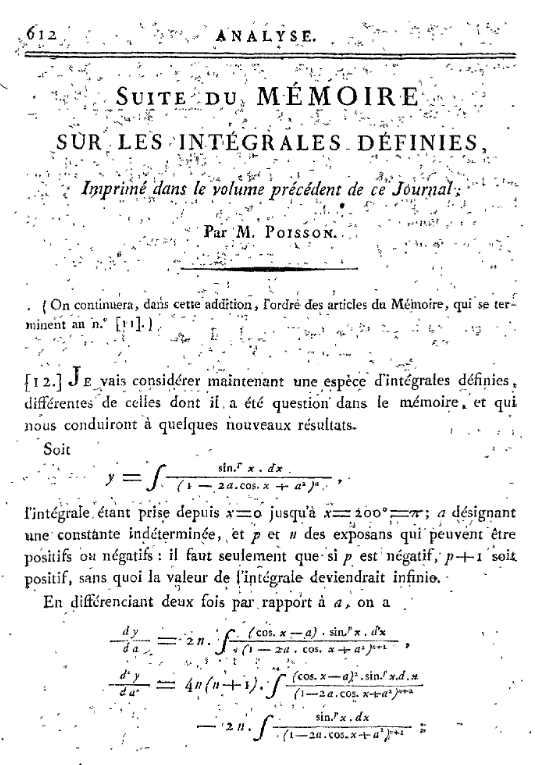
\includegraphics[scale=0.08]{illustrations/Journal_de_l_ecole_polytechnique_cahier_17_1815.png}
    % 
\includepdf[pages={3},scale=.4]{Journal_de_l_ecole_polytechnique_cahier_17_1815.pdf}
    \caption{\chevron{Suite du mémoire sur les intégrales définies}, Journal de l'École polytechnique, Cahier 17, X (1815), 612-631 (\url{https://gallica.bnf.fr/ark:/12148/bpt6k433673r/f614.item})}
\end{marginfigure}


% \printbibliography[heading=subbibintoc]


%%%%% Courbes et Surfaces %%%%%
\chapter{Géométrie, courbes et surfaces}
\labch{geometrie_courbes_et_surfaces}

\begin{itemize}
    \item Géométrie élémentaire dans l'espace
    \item Réduction, tracé de coniques/quadratiques
    \item Orthoptique d'une parabole
    \item Courbe orthoptique de l'ellipse (cercle de \textsc{Monge})
    \item Tracé du pentagone régulier à la règle et au compas
\end{itemize}
\chapter{Fonctions d'une variable réelle}
\labch{fonction_une_variable_reelle}

\marginnote[0mm]{Source : \cite{oraux_x_ens_3}}

\textsl{À partir du \textsc{xvii}$^\e$ siècle, le développment du calcul infinitésimal, motivé par de nombreux problèmes de cinématique, de mécanique, ou de calcul des variations, fait de la \say{ fonction } l'objet central des mathématiques modernes, alors que jusque là, le \say{ nombre } était la base de l'édifice mathématique. Nous devons à \textsc{Bernoulli} et \textsc{Leibniz} le terme même de \say{ fonction }: pour \textsc{Bernoulli} (1698), une fonction de la variable $x$ est \say{ une quantité formée d'une manière quelconque à partir de $x$ et de constantes }. L'écriture $y = f(x)$ est introduite par \textsc{Euler} en 1734. Les fonctions sont représentées par des courbes dans le plan et \textsc{Euler} se demande si une courbe donnée correspond toujours à une fonction. C'est lui qui distingue les courbes continues, des courbes discontinues, qui sont le plus souvent, à cette époque, des graphes de fonctions continues par morceaux. Cette double conception des fonctions, comme expressions analytiques ou comme graphes du plan, ne sera pas vraiment éclaircie avant le \textsc{xix}$^\e$ siècle (c'est \textsc{Dirichlet} qui donnera la définition moderne d'une fonction comme correspondance; il proposera ainsi (en 1837) un exemple de fonction discontinue partout, la fonction $\chi$ définie par $\chi(x) = 1$ pour $x$ rationnel et $\chi(x)=0$ pour $x$ irrationnel). \textsc{Lagrange}, cherchant à établir les fondements de l'Analyse, s'en tient au point de vue formel et refuse de se référer à toute notion de limite. Ces hésitations empêchent les mathématiciens du \textsc{xvii}$^\e$ siècle  de mener jusqu'à leur achèvement certains de leurs travaux, comme l'étude de l'équation des cordes vibrantes. C'est la génération suivante, avec entre autres \textsc{Gauss}, \textsc{Cauchy}, \textsc{Bolzano} et \textsc{Abel}, qui donnera dans la première moitié du \textsc{xix}$^\e$ siècle un statut rigoureux aux notions de convergence, de continuité, \dots Quant au concept de limite d'une fonction numérique, on doit sans doute sa première définition précise à \textsc{Weierstrass}. 
}


\newpage

\section{Point fixe d'une fonction de \texorpdfstring{$[0, 1] \rightarrow [0, 1]$}{[0, 1] dans [0, 1]}}
\begin{exercice}
    Soit $f$ une fonction dérivable sur $[0, 1]$ telle que:
    $$f(0) = f'(0) = f'(1) = 0 \text{ et } f(1) = 1.$$
    Montrer qu'il existe $c \in ]0, 1[$ tel que $f(c) = c$. 
\end{exercice}

\begin{elem_sol}
    \begin{itemize}
        \item Poser $g(x)= f(x) - x$.
        \item L'objectif est de montrer que $g$ s'annule au moins une fois sur $[0, 1]$ en montrant l'existence de $x_0$ et $x_1$ dans $[0, 1]$ tels que $g(x_0) < 0$ et $g(x_1) > 0$ pour pouvoir appliquer le \textbf{théorème des valeurs intermédiaires}.
        \item Raisonner par l'absurde sur l'existence de $x_0$ et de $x_1$ et écrire la dérivée de $f$ comme la limite de son taux d'accroissement pour aboutir à des contradictions. 
    \end{itemize}
\end{elem_sol}

\begin{marginfigure}[-8cm]
\centering
\begin{tikzpicture}
    \begin{axis}[width=6.5cm,
        axis lines=middle,
        axis line style={-latex},
        grid=major,
        xmin=-0.1, xmax=1.1,
        ymin=-0.1, ymax=1.1,
        xtick={0,1},
        xticklabels={$0$, $1$},
        ytick={0,1},
        yticklabels={$0$, $1$},
        tick style={thick},
        ticklabel style={font=\normalsize},
    ]
    \def\a{0}
    \def\b{1}
    \addplot[red,thick,samples=100,domain=\a:\b] {1/2*(1-cos(deg(pi*x^1.2)))}
    node[left,pos=1,font=\footnotesize]{\contour{white}{$\frac{1}{2}\left(1-\cos (\pi x^{6/5}) \right)$}};
    \addplot[gray,dashed,samples=100,domain=\a:\b] {x};
    \end{axis}
\end{tikzpicture}
\caption*{\centering Exemple d'une fonction vérifiant les hypothèses de l'énoncé}
\end{marginfigure}



\section{Convexité et signe}
\begin{itemize}
    \item Que peut-on dire sur une fonction concave et positive sur $\R$ ?
    \item Faire un dessin...
\end{itemize}

\section{\textsc{Rolle} à l'infini}
\begin{theo}{}
    Soit $f: \Rp \to \R$, de classe $\mathscr{C}^2$ et telle que $f(x) \xrightarrow[x \to + \infty]{} f(0)$. Alors il existe $c \in \Rpe$ et $d \in \Rp$ tel que $f'(c) = f''(d) = 0$.
\end{theo}

\section{Théorème de \textsc{Darboux}}
\begin{theo}{}
    Soit $f$ une fonction réelle, dérivable sur un intervalle $[a, b]$. Pour tout réel $k$ compris entre $f'(a)$ et $f'(b)$, il existe un réel $c \in [a, b]$ tel que $c = f'(k)$.
\end{theo}

\underline{Fonction de \textsc{Darboux}:} \\
Fonction dérivable en tout point, mais dont la dérivée est discontinue en $0$:

\begin{alignat*}{2}
    \text{Soit } f\ :\ \R\ &\longrightarrow\ \R\\
    x\ &\longmapsto\ 
    \begin{cases}
        x^2 \sin \left( \frac{1}{x^2} \right) &\text{ si } x \not= 0,\\
        0 &\text{ sinon}.
    \end{cases}
\end{alignat*}

\section{Uniforme continuité et intégrale convergente}
\begin{exercice}
    Soit $f : \Rp \to \R$ uniformément continue telle que $\int_0^{+\infty} f$ converge. Montrer que $f(x) \xrightarrow[x \to + \infty]{} 0$.
\end{exercice}

\begin{solution}
    Soit $x \in \Rp$.
    \begin{align*}
        f(x) &= f(x) - \frac{1}{2\eta_{\varepsilon}} \int_{x-\eta_{\varepsilon}}^{x+\eta_{\varepsilon}} f(t) \d t + \frac{1}{2\eta_{\varepsilon}} \int_{x-\eta_{\varepsilon}}^{x+\eta_{\varepsilon}} f(t) \d t \\
        &= \frac{1}{2\eta_{\varepsilon}} \int_{x-\eta_{\varepsilon}}^{x+\eta_{\varepsilon}} \big(f(x) - f(t) \big) \d t + \frac{1}{2\eta_{\varepsilon}} \int_{x-\eta_{\varepsilon}}^{x+\eta_{\varepsilon}} f(t) \d t \\
        |f(x)| &\leqslant \frac{1}{2\eta_{\varepsilon}} \int_{x-\eta_{\varepsilon}}^{x+\eta_{\varepsilon}} \underbrace{\big|f(x) - f(t)\big|}_{\leqslant \varepsilon} \d t + \left| \frac{1}{2\eta_{\varepsilon}} \int_{x-\eta_{\varepsilon}}^{x+\eta_{\varepsilon}} f(t) \d t \right| \\
        &\leqslant \varepsilon + \underbrace{\left|\frac{1}{2\eta_{\varepsilon}} \int_{x-\eta_{\varepsilon}}^{x+\eta_{\varepsilon}} f(t) \d t \right|}_{\mathclap{\longrightarrow 0 \text{ d'après le critère de \textsc{Cauchy}...}}}
    \end{align*}
\end{solution}

\marginnote[-7cm]{
    \begin{defi}{Continuité uniforme}
        Soit $f$ une fonction de $\R$ dans $\R$. La fonction $f$ est \emph{uniformément continue} si
        $$\forall \varepsilon > 0 \quad \exists \eta_{\varepsilon} > 0 \quad \forall(x, y) \in \R^2,$$
        $$\left( |x-y| \leqslant \eta_{\varepsilon} \implies |f(x) - f(y)| \leqslant \varepsilon \right).$$
    \end{defi}
}

\section{Lemme de \textsc{Croft}}
\marginnote[0cm]{Sources : \cite{exos_oraux} p. 259 \& \cite{oraux_x_ens_3} p. 322}

\begin{lemme}
    Soit $f : \Rp \to \R$ telle que, pour tout $a > 0$, la suite $\big(f(na) \big)_{n \geqslant 0}$ tend vers 0. \\
    Montrer que si la fonction $f$ est uniformément continue, on a $\lim\limits_{x \to + \infty} f(x) = 0$.
\end{lemme}

Sources : correction principalement de \cite{oraux_x_ens_3} avec des précisions venant de \cite{exos_oraux}.

\begin{preuve}
    L'hypothèse signifie que $f$ tend vers $0$ selon toute suite arithmétique de la forme $(na)_{n \geqslant 0}$. Lorsque la fonction est uniformément continue, on peut contrôler son comportement entre deux termes consécutifs de la suite. Plus précisément, soit $\varepsilon > 0$. La continuité uniforme de $f$ permet de choisir $\eta_\varepsilon > 0$ tel que pour tout $(x, y) \in (\Rp)^2$, 
    $$|x-y| \leqslant \eta_\varepsilon \Rightarrow |f(x) - f(y)| \leqslant \varepsilon.$$
    Puisque $\eta_\varepsilon > 0$, la suite $\big(f(n\eta_\varepsilon)\big)_{n \geqslant 0}$ tend vers $0$ par hypothèse. Fixons $N$ tel que $|f(n \eta_\varepsilon)| \leqslant \varepsilon$ pour $n \geqslant N$. \\
    Soient $x \geqslant N \eta_\varepsilon$ et $n \defeq \min\ens[\big]{ k \in \N \tq x \leqslant k \eta_\varepsilon }$ qui est bien défini. Alors $|x-n\eta_\varepsilon| \leqslant \eta_\varepsilon$. On a alors $|f(x) - f(n \eta_\varepsilon)| \leqslant \varepsilon$ de sorte que par l'inégalité triangulaire, 
    \begin{align*}
        |f(x)| &\leqslant |f(x) - f(n \eta_\varepsilon)| + |f(n \eta_\varepsilon)| \\
        &\leqslant 2 \varepsilon.
    \end{align*}
    Ceci étant valable pour tout $x \geqslant N \eta_\varepsilon$, on a bien prouvé que $f$ tend vers $0$ en $+ \infty$.
\end{preuve}  

\begin{marginfigure}[-3cm]
    \begin{tikzpicture}[scale=5]
    \draw[-latex] [thick](-0.1,0) -- (0.8,0);
    
    \draw (0,0) node [above=5pt, red,fill=white]{$N \eta_\varepsilon$};
    \draw (0,0) node {$|$};
    
    \draw (0.16,0) node [above=7pt, red,fill=white]{$\cdots$};

    \draw (0.4,0) node [above=5pt, red,fill=white]{$(n-1) \eta_\varepsilon$};
    \draw (0.4,0) node {$|$};
    
    \draw [fill] (0.6,0) circle [radius=0.3pt];
    \draw (0.6,0) node [below=2pt, blue,fill=white]{$x$};

    \draw (0.7,0) node [above=5pt, red,fill=white]{$n \eta_\varepsilon$};
    \draw (0.7,0) node {$|$};
\end{tikzpicture}
\end{marginfigure}


\begin{exercice}
    \cite{exos_oraux} (p.261)
    Déterminer les fonctions $f \in \mathscr{C}^1(\R, \R)$ telles que $f \circ f = f$.
\end{exercice}

\begin{itemize}
    \item Equation fonctionnelle
\end{itemize}
\chapter{Suites et séries de fonctions}
\labch{suites_et_series_de_fonctions}


\textsl{Le Calcul infinitésimal est l'apprentissage du maniement des \emph{inégalités} bien plus que des égalités, et on pourrait se résumer en trois mots:}
\begin{center}
        \textsc{majorer, minorer, approcher.}
\end{center}
\marginnote[0cm]{Source : V.1 Écart de deux fonctions de  \cite{calcul_infinitesimal}}
\textsl{De même qu'on cherche à \emph{approcher} un \emph{nombre} inconnu (défini par un procédé quelconque) à l'aide de nombres décimaux (ou rationnels), de même il est naturel en Analyse de chercher à \say{ approcher } une \emph{fonction} complexe inconnue (qui peut être définie par des procédés variés, somme de série, intégrale dépendant d'un paramètre, solution d'équation différentielle, etc.) à l'aide de fonctions que l'on considère comme \emph{connues} (polynômes, fonctions exponentielles, fonctions trigonométriques, etc.). Mais il faut préciser ce qu'on entend par \say{ approcher }, c'est-à-dire \say{ mesurer } en quelque sorte l'\say{ écart } de deux fonctions, de même que la valeur absolue $|x-y|$ mesure l'écart de deux nombres réels ou complexes. \\
L'idée la plus naturelle est que si une fonction $g$ \say{ approche } une fonction $f$ dans un ensemble $E$ où elles sont toutes deux définies, alors, pour chaque $x_0 \in E$, la \emph{valeur} $g(x_0)$ de $g$ doit \emph{approcher} la \emph{valeur} $f(x_0)$ de $f$ au sens usuel, c'est-à-dire que $|f(x_0)-g(x_0)|$ doit être \say{ petit }. Comme ceci doit avoir lieu en \emph{chaque} poit $x_0$ de $E$, on est conduit à prendre pour \say{ écart } de deux fonctions complexes $f$, $g$ définies dans $E$ le nombre
$$d(f, g) \defeq \sup_{x \in E} |f(x)-g(x)|.$$
Lorsqu'il s'agit de fonctions \emph{réelles} $f, g$ définies dans un intervalle $E = [a, b]$ de $\R$, l'idée d'\say{ écart } que nous venons de définir peut se concrétiser graphiquement de la façon suivante: dire que $d(f,g) \leqslant \varepsilon$ signifie que pour tout $x \in E$ on a $g(x)-\varepsilon \leqslant f(x) \leqslant g(x) + \varepsilon$, c'est-à-dire que le graphe de $f$ est \emph{tout entier} contenu dans la \say{ bande } de demi-largeur $\varepsilon$ autour du graphe de $g$. \\
Pour distinguer cette idée d'\say{ approximations } d'autres notions, nous dirons qu'il s'agit d'\emph{approximation uniforme} d'une fonction par une autre dans un ensemble $E$ où elles sont toues deux définies; il est important de remarquer que cette notion \emph{dépend essentiellement} de l'ensemble $E$ que l'on considère: si $f$ et $g$ sont toutes deux définies dans un ensemble plus grand $E'$, la relation $|f(x) - g(x)| \leqslant \varepsilon$ pour $x \in E$ n'entraîne nullement $|f(x)-g(x)| \leqslant \varepsilon$ pour $x \in E'$. \\
Étant donnés deux ensembles de fonctions $\mathscr{F}$ (les fonctions \say{ inconnues }) et $\mathscr{G}$ (les fonctions \say{ connues }) toutes définies dans un même ensemble $E$, nous dirons pour abréger qu'\emph{on peut approcher uniformément dans} $E$ les fonctions de $\mathscr{F}$ par les fonctions de $\mathscr{G}$ si, pour \emph{toute fonction} $f \in \mathscr{F}$ et \emph{tout nombre} $\varepsilon > 0$, il existe une fonction $g \in \mathscr{G}$ (dépendant de $f$ et de $\varepsilon$) telle que l'écart $d(f,g) \leqslant \varepsilon$, c'est-à-dire que 
$$|f(x) - g(x)| \leqslant \varepsilon \quad \text{pour tout } x \in E.$$
}
% https://tex.stackexchange.com/questions/383609/draw-illustration-uniform-convergence

\begin{marginfigure}[-10cm]
    % https://tex.stackexchange.com/questions/383609/draw-illustration-uniform-convergence

\begin{tikzpicture}[auto,
B/.style = {decorate,
            decoration={calligraphic brace, amplitude=3pt,
            pre=moveto,pre length=1pt,post=moveto,post length=1pt,
            raise=1mm}},
   domain = -30:30, samples=10, smooth,
     font = \footnotesize
                        ]
% coordinates
\draw[-latex] (-0.2,0) -- (6,0) node[right]{$x$};
\draw[-latex] (0,-0.2) -- (0,4) node[above]{$\textcolor{red}{f(x)}\ \textcolor{blue}{g(x)}$};
% curve
\draw[thick, red] 
    plot ({(45+\x)/15},{1+rand/5+2*cos(\x)});
    % node[coordinate,pin=0:$f$] {};
% convergence borders
\draw[dashed]  plot ({(45+\x)/15},{1.5+2*cos(\x)}) coordinate (e1);
\draw[thick, blue] plot ({(45+\x)/15},{1.0+2*cos(\x)}) coordinate (e2);
\draw[dashed]  plot ({(45+\x)/15},{0.5+2*cos(\x)}) coordinate (e3);
% labels on the left side
% \draw[B] (1,{1.25+cos(-10)}) -- node[left=1.5mm]   {$g$} ++ (0,1);
% labels on the right
\draw[B] (e1) -- node[right=1.5mm]   {$\varepsilon$} (e2);
\draw[B] (e2) -- node[right=1.5mm]   {$\varepsilon$} (e3);
% domain
\draw[dashed]   (1,{0.5+2*cos(30)}) -- (1,0)
                (5,{0.5+2*cos(30)}) -- (5,0);
\draw[very thick]    (1,0) to ["$E$" '] (5,0);
\end{tikzpicture}
\end{marginfigure}


\newpage

\section{Théorème d'approximation de \textsc{Weierstrass}}
Aussi connu sous le nom  de \emph{théorème de \textsc{Stone-Weierstrass}}

\begin{theo}
    Toute fonction continue sur un segment $[a, b]$ de $\R$ à valeurs dans $\R$ ou $\C$ est limite uniforme sur $[a, b]$ d'une suite de polynômes.
\end{theo}

\begin{preuve}
    \cite{calcul_infinitesimal} page 157.
\end{preuve} 

L'exercice suivant montre qu'il existe une suite de polynômes $(P_n)$ qui converge uniformément vers la fonction racine carrée sur $[0, 1]$.

\begin{exercice}
    \emph{Exercice 5. TD Ch. VIII}\\
    Soit la suite de fonctions définie pour tout $x \in [0, 1]$ par
    $$
    \begin{cases}
        P_0(x) &= 0,\\
        P_{n+1}(x) &= P_n (x) + \frac{1}{2} \big( x-P_n (x)^2 \big).
    \end{cases}
    $$
    Montrer que $(P_n)$ converge uniformément vers une fonction $f$ sur $[0, 1]$.
\end{exercice}

\begin{marginfigure}[-5cm]
	\begin{tikzpicture}
    \begin{axis}[width=6.5cm,
        axis lines=middle,
        grid=major,
        xmin=-0.1, xmax=1.1,
        ymin=-0.1, ymax=1.1,
        % xlabel=$x$, xlabel style={right},
        % ylabel=$y$, ylabel style={above},
        tick style={thick},
        ticklabel style={font=\normalsize},
        xtick={0, 1}, 
        ytick={0, 1},
        % legend entries={0.5x},
            legend style={
            at={(1.05,0.4)},
            anchor=north,
            legend columns=1},
            legend cell align={left}
    ]
    
    \def\a{-0.1}
    \def\b{1.1}
    
    \addplot[blue,thick,samples=100,domain=0:\b] {x^(1/2)} node (racine) {};
    %\node [left] at (racine) {$\sqrt{x}$};
    
    \addplot[red,thick,samples=100,domain=\a:\b] {0} node (P0) {};
    %\node [left] at (P0) {$P_0$};
    
    \addplot[red,thick,samples=100,domain=\a:\b] {x/2} node (P1) {};
    %\node [anchor=north east] at (P1) {$P_1$};
    
    \addplot[red,thick,samples=100,domain=\a:\b] {-1/8*x^2+x} node (P2) {};
    %\node [left] at (P2) {$P_2$};
    
    \addplot[red,thick,samples=100,domain=\a:\b] {-1/128*x^4+1/8*x^3-5/8*x^2+3/2*x} node (P3) {};
    %s\node [left] at (P3) {$P_3$};
    
    \addplot[red,thick,samples=100,domain=\a:\b] {-1/128*x^4+1/8*x^3-5/8*x^2+3/2*x + 1/2*(x-(-1/128*x^4+1/8*x^3-5/8*x^2+3/2*x)^2)} node (P4) {};
    \end{axis}
\end{tikzpicture}


%import matplotlib.pyplot as plt
%import numpy as np
%from numpy.polynomial import Polynomial

%PAS = 1e-3
%n = 8
%X = np.arange(0, 1, PAS)


%P = Polynomial([0])
%plt.plot(X, P(X))

%for k in range(n):
%    P = P + 1/2 * (Polynomial([0, 1]) - P ** 2)
%    plt.plot(X, P(X))

%racine = [np.sqrt(x) for x in X]
%plt.plot(X, racine, 'r')
%plt.show()

\end{marginfigure}

Peut-on génraliser à $\R$ ? \dots

\begin{tcolorbox}
    Si $(P_n)_{n \in \N}$ est une suite de polynômes convergeant uniformément sur $\R$ vers une fonction $f$, alors $f$ est un polynôme.
\end{tcolorbox}

\begin{preuve}
    Source : \cite{exos_oraux} \& \cite{maths-france}. \\
    Soit $(P_n)_{n \in \N}$ une suite de polynômes convergeant uniformément sur $\R$ vers une fonction $f$. \\
    D'après la critère de \textsc{Cauchy} uniforme, il existe un rang $n$ tel que pour tout $p \in \N$, 
    $$\Ninf{P_{n+p} - P_n} \leqslant 1.$$
    La fonction polynomiale $P_{n+p} - P_n$ est donc bornée sur $\R$ autrement dit elle est constante. On a alors,
    $$\forall (p, x) \in \N \times \R,\ P_{n+p}(x) = P_n(x) + P_{n+p}(0) - P_n(0) \xrightarrow[p \to + \infty]{} P_n(x) + f(0) - P_n(0)$$
    donc par unicité de la limite simple, $f : x \mapsto P_n(x) + f(0) - P_n(0)$, qui définit bien une fonction polynomiale. 
\end{preuve}

\section{Approximation polynomiale de \textsc{Bernstein}}
\textsc{Bernstein} a donné une démonstration constructive et probabiliste du théorème de \textsc{Weierstrass} sur $[0, 1]$, en prouvant qu'on pouvait prendre : 

\begin{defi}{Polynôme de \textsc{Bernstein}}
    Le polynôme de \textsc{Bernstein} d'ordre $n$ associé à la fonction $f$ est le polynôme
    \begin{equation} \label{1}
        \Bernstein_n(f)(x) \defeq \sum_{p=0}^{n} f \left( \frac{p}{n} \right) \binom{n}{p} x^p (1-x)^{n-p}
    \end{equation}
\end{defi}

\marginnote[0cm]{Source : \cite{acamanes} \href{https://acamanes.github.io/psi/psi_doc/exos_e08.pdf}{(Exercice 10. TD VIII)}}
\begin{theo}{}
    Soit $f$ une fonction continue sur $I \defeq [0, 1]$. 
    La suite $\big( \Bernstein_n(f) \big)_n$ converge uniformément vers la fonction $f$ sur $I$.
\end{theo}

Nous allons voir deux démonstrations de ce théorème.

\begin{preuve}
    Le démonstration qui suit est celle proposée dans \cite{calcul_infinitesimal} page 159 dont quelques étapes techniques ont été détaillées. \\
    Nous partirons de l'identité
    \begin{equation}
        1 = (1-t+t)^n = \sum_{p=0}^n \binom{n}{p} (1-t)^{n-p}t^p.
    \end{equation}
    On déduit de cette relation que pour toute fonction bornée $f$ définie dans $I$, on a
    \begin{equation} \label{2}
        |\Bernstein_n(f)(t)| \leqslant \sup_{t \in I} |f(t)| \cdot \left(\sum_{p=0}^n \binom{n}{p} (1-t)^{n-p}t^p \right) = d(0, f)
    \end{equation}
    puisque les fonctions $\binom{n}{p}(1-t)^{n-p}t^p$ prennent des \emph{valeurs} $\geqslant 0$ \emph{dans} $I$. \\
    Étant donné $\varepsilon > 0$, on sait que pour toute fonction continue $f$ dans $I$, il existe, en vertu du théorème de \textsc{Weierstrass}, un polynôme $P$ tel que $d(f, P) \leqslant \varepsilon$; on conclut alors de (\ref{2}) que
    \begin{equation} \label{3}
        d(\Bernstein_n(f), \Bernstein_n(P)) \leqslant d(f, P) \leqslant \varepsilon.
    \end{equation}
    Par suite, pour $t \in I$,
    \begin{align*}
        |f(t)-\Bernstein_n(f)(t)| &\leqslant |f(t) - \Bernstein_n(P)(t)| + \underbrace{|\Bernstein_n(P)(t) - \Bernstein_n(f)(t)|}_{\leqslant \varepsilon \text{ d'après (\ref{3})}} \\
        &\leqslant \underbrace{|f(t) - P(t)|}_{\leqslant \varepsilon} + |P(t) - \Bernstein_n(P)(t)| + \varepsilon
    \end{align*}
    Ainsi, par passage à la borne supérieure sur $I$, on obtient
    \begin{equation} \label{5}
        d(f, \Bernstein_n(f)) \leqslant 2 \varepsilon + d(P, \Bernstein_n(P)).
    \end{equation}
    Si l'on prouve le théorème lorsque $f$ est un \emph{polynôme}, il sera donc vrai pour toute fonction continue dans $I$. Par linéarité, il suffit donc de le prouver lorsque $f(t) = t^m$. En fait, nous allons voir, par récurrence sur $m$, que l'on a, en posant $f_m(t) = t^m$, pour $n \geqslant m$, 
    \begin{equation} \label{6}
        \Bernstein_n(f_m)(t) = t^m + \frac{1}{n}Q_{m,n}(t)
    \end{equation}
    où $Q_{m,n}$ est un polynôme de degré inférieur à $m-1$, dont les coefficients sont majorés en valeur absolue par un nombre $A_m$ \emph{indépendant de} $n$. \\
    La formule (\ref{6}) se réduit à (\ref{2}) pour $m=0$, avec $Q_{0,n}(t) = 0$. Supposons-la vérifiée pour un entier $m$ et dérivons par rapport à $t$; en vertu de la défition (\ref{1}), on obtient, pour $n \geqslant m+1$, 
    \begin{equation} \label{7}
        -\sum_{p=0}^{n-1} \binom{n}{p} \frac{p^m}{n^m}(n-p)(1-t)^{n-p-1}t^p + \sum_{p=1}^n \binom{n}{p} \frac{p^{m+1}}{n^m}(1-t)^{n-p}t^{p-1} = mt^{m-1} + \frac{1}{n} Q'_{m,n}(t).
    \end{equation}
    Comme $(n-p) \binom{n}{p} = n \binom{n-1}{p}$, le premier terme du premier membre de (\ref{7}) est égal à 
    $$-n \Bernstein_{n-1}(f_m)(t) = -nt^m - \frac{n}{n-1}Q_{m, n-1}(t).$$ 
    Multipliant les deux membres de (\ref{7}) par $\frac{t}{m}$, on obtient donc, en vertu de la définition des polynômes de \textsc{Bernstein},
    \begin{equation*}
        -\frac{n}{m} t^{m+1} - \frac{nt}{m(n-1)}Q_{m, n-1}(t) + \frac{n}{m} \underbrace{\sum_{p=1}^n \binom{n}{p} \frac{p^{m+1}}{n^{m+1}}(1-t)^{n-p}t^p}_{\Bernstein_n(f_{m+1})(t)} = t^m + \frac{t}{mn}Q'_{m,n}(t)\\
    \end{equation*}
    soit en réarrangeant les termes et en multipliant l'égalité par $\frac{m}{n}$;
    \begin{align*}
        \Bernstein_n(f_{m+1})(t) &= t^{m+1} + \frac{m}{n}t^m + \frac{t}{n^2}Q'_{m,n}(t) + \frac{t}{n-1} Q_{m, n-1}(t) \\
        &= t^{m+1} + \frac{1}{n}Q_{m+1, n}(t)
    \end{align*}
    avec $Q_{m+1, n}(t) = mt^m + \frac{1}{n}t Q'_{m,n}(t) + \frac{n}{n-1}t Q_{m,n-1}(t)$. \\
    Comme, par hypothèse, $Q_{m,n}$ est de degré inférieur à $m-1$, le polynôme $Q_{m+1, n}$ est bien de degré inférieur à $m$. \\
    Les coefficients de $\frac{1}{n}t Q'_{m,n}(t)$ sont majorés en valeur absolue par $\frac{m-1}{n}A_m \leqslant (m-1)A_m$ ... \textcolor{red}{A FINIR}
    et cela prouve (\ref{6}) par récurrence, avec
    $$A_{m+1} \leqslant 3 \sup(m, (m-1) A_m).$$
\end{preuve}

Le sujet \textsc{x/ens psi 2018} propose une démonstration élégante de ce résultat d'analyse pure en passant par les probabilités. (Je crois que la version du TD est un peu différente).
Préciser les hypothèses sur $f$.
\begin{exercice}        
    Soit $x \in ]0, 1[$ et $n \in \Ne$. On considère $X_1, \dots, X_n$ des variables aléatoires mutuellement indépendantes et suivant toutes la même loi de \textsc{Bernoulli} de paramètre $x$. On pose
    $$S_n = \frac{X_1 + \cdots + X_n}{n}.$$
    \begin{enumerate}
        \item Exprimer $\E(S_n)$, $\V(S_n)$ et $\E(f(S_n))$ en fonction de $x$, $n$ et du polynôme $\Bernstein_n(f)$.
        \item En déduire les inégalités:
        $$\sum_{k=0}^{n} \left| x- \frac{k}{n} \right| \binom{n}{k} x^k (1-x)^{n-k} \leqslant \V(S_n)^{1/2} \leqslant \frac{1}{2\sqrt{n}}.$$
        \item Montrer que $\lambda^\alpha \leqslant 1+\lambda$ pour tout réel $\lambda > 0$ et en déduire l'inégalité:
        $$\left|x-\frac{k}{n} \right|^\alpha \leqslant n^{-\alpha/2} \Bigg(1 + \sqrt{n} \left|x - \frac{k}{n} \right| \Bigg)$$
        pour tout $x \in ]0, 1[, n \in \Ne$ et $k \in \llbracket 1, n \rrbracket$.
        \item Soit $n \in \Ne$. Montrer que 
        $$\Ninf{f-\Bernstein_n(f)} \leqslant \frac{3k}{2} \frac{1}{n^{\alpha/2}}.$$
        Conclure.
    \end{enumerate}
\end{exercice}

\marginnote[0cm]{
    \begin{prop}{\note Somme de \textsc{Bernoulli} indépendantes}
        La somme de $n$ variables aléatoires discrètes indépendantes suivant la même loi de \textsc{Bernoulli} de paramètre $p$ suit une loi binomiale de paramètres $(n, p)$. 
    \end{prop}
    La démontration est immédiate en passant par les fonctions génératrices.
}

\begin{preuve}
    Soit $x \in [0, 1]$. On considère une suite de variables aléatoires $(X_n)_n$ indépendantes identiquement distribuées de loi de \textsc{Bernoulli} $\mathscr{B}(x)$. Ainsi, $S_n \defeq \sum\limits_{i=1}^n X_i$ suit une loi binomiale $\mathscr{B}(n, x)$ \note et par le théorème de transfert
    $$\E \left[ f\left( \frac{S_n}{n} \right) \right] = \sum_{p=0}^n \binom{n}{p} f \left( \frac{p}{n} \right) (1-x)^{n-p} x^p = \Bernstein_n(f)(x).$$
    On va chercher à utiliser la convergence en probabilité de $\frac{S_n}{n}$ vers $x$. \\
    Soit $\varepsilon > 0$. La fonction $f$ étant continue sur le compact $[0, 1]$ donc d'après le théorème de \textsc{Heine} \note, elle y est uniformément continue i.e.
    $$\exists \eta > 0, |x-y| \leqslant \eta \Rightarrow |f(x) - f(y)| \leqslant \varepsilon.$$
    \marginnote[-4cm]{
        \begin{theo}{\note Théorème de \textsc{Heine}}
             Une fonction continue sur un segment, plus généralement sur un compact, y est uniformément continue. 
        \end{theo}
    }
    On va alors scinder en deux. On a
    \marginnote[0cm]{On retrouve cette méthode de séparation avec la fonction indicatrice dans la démonstration de l'inégalité de \textsc{Markov}.}
    \begin{align*}
        |f(x) - \Bernstein_n(f)(x)| &= \left| \E \left[ f(x) - f\left( \frac{S_n}{n} \right) \right] \right| \leqslant \E \left[ \left| f(x) - f \left( \frac{S_n}{n} \right) \right| \right] \\
        &\leqslant \E \left[ \left| f(x) - f \left( \frac{S_n}{n} \right) \right| \mathds{1}_{\left| x - \frac{S_n}{n} \right| < \eta} + \left| f(x) - f \left( \frac{S_n}{n} \right) \right| \mathds{1}_{\left| x - \frac{S_n}{n} \right| \geqslant \eta} \right] \\
        \text{par linéarité de l'espérance } &\leqslant \E \left[ \left| f(x) - f \left( \frac{S_n}{n} \right) \right| \mathds{1}_{\left| x - \frac{S_n}{n} \right| < \eta} \right] + \E \left[ \left| f(x) - f \left( \frac{S_n}{n} \right) \right| \mathds{1}_{\left| x - \frac{S_n}{n} \right| \geqslant \eta} \right] \\
        &\leqslant \varepsilon + 2 \Ninf{f} \E \left[ \mathds{1}_{\left| x - \frac{S_n}{n} \right| \geqslant \eta} \right] \\
        \text{par l'espérance d'une indicatrice } &\leqslant \varepsilon + 2 \Ninf{f} \P \left( \left| x - \frac{S_n}{n} \right| \geqslant \eta \right).
    \end{align*}
    On utilise alors l'inégalité de \textsc{Bienaymé}-\textsc{Tchebychev} \note (on rappelle que $\E[S_n/n] = x$)
    \marginnote[-2cm]{
        \begin{theo}{\note Inégalité de \textsc{Bienaymé}-\textsc{Tchebychev}}
            Soit $X$ une v.a.r.d. admettant un moment d'ordre $2$,
            $$\forall \varepsilon > 0,\ \P \big(|X-\E[X]| \geqslant \varepsilon \big) \leqslant \frac{\V(X)}{\varepsilon^2}.$$
        \end{theo}
    }
    \begin{align*}
        |f(x) - \Bernstein_n(f)(x)| &\leqslant \varepsilon + 2 \Ninf{f} \frac{\V(S_n/n)}{\eta^2} \\
        &\leqslant \varepsilon + 2 \Ninf{f} \frac{\V(S_n)}{n^2 \eta^2} \\
        &\leqslant \varepsilon + 2 \Ninf{f} \frac{x(1-x)}{n \eta^2} \\
        &\leqslant \varepsilon + \Ninf{f} \frac{1}{2 n \eta^2} \text{ indépendant de $x$}.
    \end{align*}
    Ainsi, on a $\lim \sup_n \Ninf{f - \Bernstein_n(f)} \leqslant \varepsilon$, et on a en faisant tendre $\varepsilon$ vers $0$:
    $$\Ninf{f - \Bernstein_n(f)} \xrightarrow[n \to + \infty]{} 0.$$
\end{preuve}

\begin{remarque}
    Ce résultat peut être étendu à toute fonction continue sur un segment $[a, b]$ en posant
    $$\forall x \in [0, 1], f(x) = g \big( (b-a)x + a \big).$$
    La fonction $x \mapsto (b-a)x + a$ est un homéomorphisme de $[0, 1]$ sur $[a, b]$.
\end{remarque}

\section{Intégration d'une série de fonctions}
Soit $S:x \to \sum\limits_{n=1}^{+\infty} \frac{(-1)^n}{1+n^2 x^2}$.
\begin{itemize}
    \item Donner l'ensemble de définition de $S$ et donner un équivalent en $+\infty$.\\
    $\blacktriangleright$  $D_S = \Re$.\\
    $\blacktriangleright$ On se doute que $S$ \textbf{se comporte comme} $\frac{1}{x^2}$ en $+\infty$. L'idée est donc de déterminer la limite de $x^2 S(x)$ en $+\infty$. Le \textbf{théorème d'interversion des limites} permet d'affirmer que cette limite est finie et qu'elle est égale à $c = \sum\limits_{n=1}^{+\infty} \frac{(-1)^n}{n^2}$. Une séparation des termes pairs et impairs de la somme (et le résultat du \href{https://fr.wikipedia.org/wiki/Problème_de_Bâle}{problème de Bâle}) permet de montrer que $c = -\frac{\pi^2}{12}$ et donc $S(x) \sim_{+\infty} -\frac{\pi^2}{12x^2}$.
    \item Montrer que $S$ est intégrable sur $\Rpe$ et calculer $\int_0^{+\infty} S(t) \mathrm{d}t$.\\
    $\blacktriangleright$ Comme $S$ est une série alternée, on peut lui appliquer le \textbf{théorème des séries alternées} et écrire que 
    $$|S(x)| \leqslant \frac{1}{1+x^2} \text{ (majoration du reste d'ordre 1)}$$
    L'intégrabilité du majorant sur $\Rpe$ assure celle de $S$ sur cet ensemble. \textcolor{green}{Est-ce que l'intégrabilité sur R+* des termes de la somme et leur CU vers $S$ impliquent l'ingrabilité de $S$ sur cet ensemble ? c.f. théorème de la convergence dominée peut-être...}\\
    $\blacktriangleright$ L'interversion série/intégrale permet de montrer que $\int_0^{+\infty} S(t) \d t = \frac{\pi}{2} \sum\limits_{n=1}^{+\infty} \frac{(-1)^n}{n} = -\frac{\pi}{2} \ln(2)$ (c.f. \nameref{deux_sommes}).\\
    \textcolor{green}{Dans la correction (p. 374), on effectue le calcul sur une somme partielle et on détermine ensuite la limite de cette somme. J'avais naïvement travailler avec l'intégrale jusqu'en +infini et la somme aussi, \textbf{est-ce licite ?}}.
\end{itemize}

\section{Équivalent d'une série de fonctions}
\begin{exercice}
    On pose $f(x) = \sum\limits_{n=1}^{+\infty}\frac{x}{n(1+nx^2)}$. Donner un équivalent de $f$ et $0^+$.
\end{exercice}

\begin{solution}
    Éffectuer une comparaison série/intégrale aux termes de la somme pour encadrer $f$ (ne pas oublier de justifier l'intégrabilité des fonctions sur $[1, +\infty[$):
    $$\int_{2}^{+\infty} \frac{x}{t(1+tx^2)} \d t + \frac{x}{1+x^2} \leqslant f(x) \leqslant \int_{1}^{+\infty} \frac{x}{t(1+tx^2)} \d t + \frac{x}{1+x^2}.$$ 
    Décomposer les intégrandes en éléments simples et calculer les intégrales:
    $$-2x \ln(x) + o_0(x\ln(x)) \leqslant f(x) \leqslant -2x \ln(x) + o_0(x\ln(x))$$
    Finalement, 
    $$f(x) \isEquivTo{0^+} -2x\ln(x)$$
\end{solution}

\section{Série de fonctions continues dont la somme est discontinue}
\begin{prop}{}
    \marginnote[0cm]{Source : \cite{contre-exemples} p.257}
    Soit la suite $(f_n)_{n \geqslant 0}$ d'applications continues de $[0,1]$ dans $\R$, de terme général
    \begin{alignat*}{2}
        f_n\ :\ [0,1]\ &\longrightarrow\ \R\\
        x\ &\longmapsto\ f_n(x) = (1-x)x^n.
    \end{alignat*}
    La somme des $f_n$ est discontinue.
\end{prop}

\begin{preuve}
    Pour tout point $x$ de $[0,1[$, la série $\sum f_n(x)$ est le produit par $(1-x)$ d'une série géométrique de raison $x$ où $0 \leqslant x < 1$, donc elle converge et sa somme est égale à $(1-x)/(1-x) = 1$. De plus $f_n(1) = 0$ pour tout entier naturel $n$. La série de fonctions $\sum f_n$ converge donc simplement sur le segment $[0,1]$ et sa somme est l'application 
    \begin{alignat*}{2}
        S\ :\ [0,1]\ &\longrightarrow\ \R\\
        x\ &\longmapsto\ S(x) =
        \begin{cases}
            1 &\text{ si } x \in [0,1[,\\
            0 &\text{ si } x = 1,
        \end{cases}
    \end{alignat*}
    qui est discontinue en $1$.
\end{preuve}


\section{Fonction \texorpdfstring{$\zeta$}{zêta} alternée}
\marginnote[0cm]{Source : \cite{acamanes} \href{https://acamanes.github.io/psi/psi_doc/exos_e08.pdf}{(Exercice 13. TD VIII)}}
On définit la fonction $\zeta$ alternée $F$ comme suit
$$F(x) = \sum_{n=1}^{+ \infty} \frac{(-1)^{n-1}}{n^x}.$$
\begin{itemize}
    \item Déterminer l'ensemble de défintion de $F$ et trouver une relation entre $F$ et $\zeta$.
    \begin{itemize}
        \item Calculer $\zeta(x) - F(x)$ pour trouver que $\zeta(x) = \frac{1}{1-2^{1-x}} F(x)$.
    \end{itemize}
    \item Déterminer $\displaystyle \lim_{x \to 1} (x-1) \zeta(x)$.
    \begin{itemize}
        \item En comparant $\zeta$ à une intégrale, on peut montrer que $\frac{1}{1-x} \leqslant \zeta(x) \leqslant \frac{1}{1-x} + 1$.
    \end{itemize}
    \item On peut aussi procéder de la manière suivante: $\zeta$ est décroissante sur $]1, +\infty[$ donc $\zeta$ admet une limite $\ell \in \Rp \cup \{ + \infty \}$ en $1$.\\
        $\blacktriangleright$ Si $\ell \in \Rp$, par passage à la limite dans l'inégalité $\zeta(x) \geqslant \sum\limits_{n=1}^{N} \frac{1}{n^x}$, $$\ell \geqslant \sum\limits_{n=1}^{N} \frac{1}{n} \xrightarrow[N \to + \infty]{} +\infty.$$ 
        Donc $\ell = + \infty$ et $\displaystyle \lim_{x \to 1} \zeta(x) = +\infty$. 
    \item Déterminer $\displaystyle \lim_{x \to +\infty} F(x)$ ainsi qu'un équivalent de $\zeta$ en $+\infty$.
    \begin{itemize}
        \item On peut montrer que (\textcolor{green}{à détailler}) $\zeta(x) \sim_{+ \infty} 1$.
    \end{itemize}
\end{itemize}

\section{Fonctions continues nulle part dérivables}
\marginnote[0cm]{
\emph{\say{ Je me détourne avec effroi et horreur de cette plaie lamentable des fonctions continues qui n'ont point de dérivées. }} \\
\hspace*{\fill} Charles \textsc{Hermite} (1893) \\
\emph{\say{ C’est un cas où il est vraiment naturel de penser à ces fonctions continues sans dérivées que les mathématiciens ont imaginées, et que l’on regardait à tort comme de
simples curiosités mathématiques, puisque l’expérience peut les suggérer. }} \\
\hspace*{\fill} Jean \textsc{Perrin} \sidenote{Physicien, chimiste et homme politique français (1870 - 1942), prix Nobel de physique 1926.}, au sujet du mouvement brownien.
}

\cite{contre-exemples} p. 160 \\
Jusqu'à la moitié du \textsc{xix}$^\me$ siècle, on pensait généralement qu'une fonction continue était dérivable sauf peut-être en quelques points. \textsc{Ampère} prétendit même l'avoir démontré en 1806. \textsc{Bolzano} donne vers 1830 un exemple de fonction continue, mais dérivable nulle part; cependant ses écrits restent méconnus. En 1854, Bernhard \textsc{Riemann}, propose sans preuve, la fonction:
$$R:x \mapsto R(x) \defeq \sum_{n=1}^{+\infty} \frac{\sin(n^2 x)}{n^2}.$$
Karl \textsc{Weierstrass} se déclare incapable de la démontrer. Il faut attendre 1971 pour savoir que $R$ n'est pas dérivable sauf en certains points. En 1872, Karl \textsc{Weierstrass} démontre que si $a$ et $b$ sont des réels tels que $a > 0$, $b > 0$ et $ab > 1 + \frac{3 \pi}{2}$, la fonction:
$$f : x \mapsto f(x) \defeq \sum_{n=1}^{+\infty} b^n \cos(a^n x)$$
est continue sur $\R$ et n'est dérivable en aucun point de $\R$.

\textbf{Notations.}\\
On note $E$ l'ensemble des fonctions continues sur $[0, 1]$ et $F$ l'ensemble des fonctions continues sur $[0, 1]$, nulle part dérivables sur $[0, 1]$. 

\begin{theo}{}
    L'ensemble $F$ est non vide.
\end{theo}

\begin{preuve}
    \marginnote[0cm]{\url{https://share.miple.co/content/XEZ7y9BayeSN1}}
    Notons:
    \begin{itemize}
        \item $\forall x \in \Rp, \Delta(x) \defeq \min\limits_{n \in \N} |x - n|$,
        \item $\forall x \in \Rp, \Delta_n(x) \defeq \frac{\Delta(2^n x)}{2^n x}$,
        \item $\forall x \in [0, 1], W(x) \defeq \sum\limits_{n=0}^\infty \Delta_n(x)$.
    \end{itemize}
    Nous allons montrer que la fonction $W$ est un élément de $F$.
    \begin{itemize}
    \item[$\rhd$] \textbf{Continuité.} La fonction $\Delta$ est minimale sur $\N$ où elle vaut $0$, et est maximale sur $\N + \frac{1}{2}$ où elle vaut $\frac{1}{2}$, d'où $\Ninf{\Delta} \leqslant \frac{1}{2}$ et donc $\Ninf{\Delta_n} \leqslant \frac{1}{2^{n+1}}$. Les fonction $\Delta_n$ étant continues et $\sum \Delta_n$ convergeant normalement, la fonction $W$ est continue. 
    \item[$\rhd$] \textbf{Non-dérivabilité.} Soit $x \in [0, 1]$. On note, pour tout $p \in \N$, 
    $$x_p \defeq \frac{\lfloor 2^p x \rfloor}{2^p} \text{ et } y_p \defeq x_p + \frac{1}{2^p}.$$ 
    Étudions la limite de $\limits \frac{W(x_p) - W(y_p)}{x_p - y_p}$ quand $p$ tend vers $+ \infty$:
    \begin{itemize}
        \item Si $n \geqslant p$, alors $2^n x_p$ et $2^n y_p$ sont des entiers. Donc $\Delta_n(x_p) = \Delta_n(y_p) = 0$ et $\frac{\Delta_n(x_p) - \Delta_n(y_p)}{x_p - y_p} = 0$.
        \item Si $n < p$, alors $x_p, y_p \in I_1 \defeq \left[ x_n, \frac{x_n + y_n}{2} \right]$ ou $x_p, y_p \in I_2 \defeq \left[ \frac{x_n + y_n}{2}, y_n \right]$. $\Delta_n$ a une pente $1$ sur $I_1$ et une pente $-1$ sur $I_2$. Donc $\frac{\Delta_n(x_p) - \Delta_n(y_p)}{x_p - y_p} = (-1)^{\lfloor 2^{n+1} x \rfloor}$. 
    \end{itemize}
    Donc:
    $$\frac{W(x_p) - W(y_p)}{x_p - y_p} = \sum_{n=0}^{p-1} (-1)^{\lfloor 2^{n+1} x \rfloor}.$$
    Notons $r_p \defeq \frac{W(y_p) - W(x_p)}{y_p - x_p}$. La suite $(r_p)_{p \in \N}$ ne converge par puisque $r_{p+1} - r_p = (-1)^{\lfloor 2^{n+1} x \rfloor}$ ne tend pas vers $0$. \\
    Comme $x_p \xrightarrow[p \to \infty]{} x$ et $y_p \xrightarrow[p \to \infty]{} x$, on en conclut que $W$ n'est pas dérivable en $x$ et donc est nulle part dérivable sur $[0, 1]$.
    \end{itemize}
\end{preuve}

\subsection{Courbe du blancmanger ou de \textsc{Takagi}}

\marginnote[0cm]{\cite{contre-exemples} p. 160}
En 1903, le mathématicien japonais Teiji \textsc{Takagi} (1875-1960) propose les fonctions:
$$f : x \mapsto f(x) \defeq \sum_{n=0}^{+ \infty} b^n g(a^n x)$$
où $g$ est la fonction de $g : x \mapsto d(x, \Z)$ (distance de $x$ à $\Z$) de $\R$ dans $\R$ et $a$ et $b$ des réels tels que $0 < b < 1$ et $a \leqslant 4$. Lorsque de plus $ab > 2$, la fonction $f$ a des dérivées supérieures égales à $+\infty$ et inférieures égales à $- \infty$ en tout point de $\R$. \\

\marginnote[0cm]{Alain \textsc{Camanes} DS MPSI1 10/01/2015}
La fonction de \textsc{Takagi} a été introduite par Teiji \textsc{Takagi} en 1903 motivé par les fonctions nulle part dérivables de \textsc{Weierstrass} après une visite en Allemagne de 1897 à 1901. \\
Une variante de la fonction de \textsc{Takagi}, utilisant la base $10$ et non la base $2$, a été introduite par \textsc{Van der Waerden} en  1930. Bien que non différentiables, ces fonctions possèdent des dérivées infinies en de nombreux points (tout comme la fonction de \textsc{Weierstrass}). C'est pourquoi \textsc{Knopp} a introduit en 1918 une variante de la fonction de \textsc{Takagi} qui, en tout point, n'admet ni de dérivée finie ni de dérivée infinie.

\begin{figure*}[h!]
    \centering
    \begin{tikzpicture}[scale=0.8]

    \begin{scope}[local bounding box=struct, scale=3]
        \draw[red] (0, 0) -- (1/2, 1/2) -- (1, 0);
    \end{scope}
    
    \begin{scope}[shift={($(struct.east)+(1,-3/4)$)}, scale=3]
        \draw[dashed] (1/4, 1/4) -- (1/2, 1/2) -- (3/4, 1/4);
        \draw[red] (0, 0) -- (1/4, 1/4) -- (1/2, 0) -- (3/4, 1/4) -- (1, 0);
        \draw (0, 0) -- (1/4, 1/2) -- (3/4, 1/2) -- (1, 0);
    \end{scope}
    
    \begin{scope}[shift={($(struct.east)+(5,-3/4)$)}, scale=3]
        \draw[dashed] (0, 0) -- (1/4, 1/2) -- (3/4, 1/2) -- (1, 0);
        \draw[red] (0, 0) -- (1/8, 1/8) -- (1/4, 0) -- (3/8, 1/8) -- (1/2, 0) -- (5/8, 1/8) -- (6/8, 0) -- (7/8, 1/8) -- (1, 0);
        \draw (0, 0) -- (1/8, 3/8) -- (3/8, 5/8) -- (1/2, 1/2) -- (5/8, 5/8) -- (7/8, 3/8) -- (1, 0);
    \end{scope}
    
    \begin{scope}[shift={($(struct.east)+(9,-3/4)$)}, scale=3]
        \draw[dashed] (0, 0) -- (1/8, 3/8) -- (3/8, 5/8) -- (1/2, 1/2) -- (5/8, 5/8) -- (7/8, 3/8) -- (1, 0);
        \draw[red] (0, 0) -- (1/16, 1/16) -- (2/16, 0) -- (3/16, 1/16) -- (4/16, 0) -- (5/16, 1/16) -- (6/16, 0) -- (7/16, 1/16) -- (8/16, 0) -- (9/16, 1/16) -- (10/16, 0) -- (11/16, 1/16) -- (12/16, 0) -- (13/16, 1/16) -- (14/16, 0) -- (15/16, 1/16) -- (1, 0);
        \draw (0, 0) -- (1/16, 4/16) -- (3/16, 1/2) -- (4/16, 1/2) -- (5/16, 5/8) -- (7/16, 5/8) -- (1/2, 1/2) -- (9/16, 5/8) -- (11/16, 5/8) -- (12/16, 1/2) -- (13/16, 1/2) -- (15/16, 4/16) -- (1, 0);
    \end{scope}
\end{tikzpicture}
    \caption*{\centering Construction graphique}
\end{figure*}

\begin{figure}[h!]
    \centering
	% This file was created with tikzplotlib v0.10.1.
\begin{tikzpicture}

\begin{axis}[
title={Courbe du blanc-manger d'ordre 9},
xtick={0, 1/2, 1}, 
ytick={0, 1/2, 1}
]
\addplot [line width=0.32pt, cyan]
table {%
0 0
0.001953125 0.017578125
0.00390625 0.03125
0.005859375 0.044921875
0.0078125 0.0546875
0.009765625 0.068359375
0.01171875 0.078125
0.013671875 0.087890625
0.015625 0.09375
0.017578125 0.107421875
0.01953125 0.1171875
0.021484375 0.126953125
0.0234375 0.1328125
0.025390625 0.142578125
0.02734375 0.1484375
0.029296875 0.154296875
0.03125 0.15625
0.033203125 0.169921875
0.03515625 0.1796875
0.037109375 0.189453125
0.0390625 0.1953125
0.041015625 0.205078125
0.04296875 0.2109375
0.044921875 0.216796875
0.046875 0.21875
0.048828125 0.228515625
0.05078125 0.234375
0.052734375 0.240234375
0.0546875 0.2421875
0.056640625 0.248046875
0.05859375 0.25
0.060546875 0.251953125
0.0625 0.25
0.064453125 0.263671875
0.06640625 0.2734375
0.068359375 0.283203125
0.0703125 0.2890625
0.072265625 0.298828125
0.07421875 0.3046875
0.076171875 0.310546875
0.078125 0.3125
0.080078125 0.322265625
0.08203125 0.328125
0.083984375 0.333984375
0.0859375 0.3359375
0.087890625 0.341796875
0.08984375 0.34375
0.091796875 0.345703125
0.09375 0.34375
0.095703125 0.353515625
0.09765625 0.359375
0.099609375 0.365234375
0.1015625 0.3671875
0.103515625 0.373046875
0.10546875 0.375
0.107421875 0.376953125
0.109375 0.375
0.111328125 0.380859375
0.11328125 0.3828125
0.115234375 0.384765625
0.1171875 0.3828125
0.119140625 0.384765625
0.12109375 0.3828125
0.123046875 0.380859375
0.125 0.375
0.126953125 0.388671875
0.12890625 0.3984375
0.130859375 0.408203125
0.1328125 0.4140625
0.134765625 0.423828125
0.13671875 0.4296875
0.138671875 0.435546875
0.140625 0.4375
0.142578125 0.447265625
0.14453125 0.453125
0.146484375 0.458984375
0.1484375 0.4609375
0.150390625 0.466796875
0.15234375 0.46875
0.154296875 0.470703125
0.15625 0.46875
0.158203125 0.478515625
0.16015625 0.484375
0.162109375 0.490234375
0.1640625 0.4921875
0.166015625 0.498046875
0.16796875 0.5
0.169921875 0.501953125
0.171875 0.5
0.173828125 0.505859375
0.17578125 0.5078125
0.177734375 0.509765625
0.1796875 0.5078125
0.181640625 0.509765625
0.18359375 0.5078125
0.185546875 0.505859375
0.1875 0.5
0.189453125 0.509765625
0.19140625 0.515625
0.193359375 0.521484375
0.1953125 0.5234375
0.197265625 0.529296875
0.19921875 0.53125
0.201171875 0.533203125
0.203125 0.53125
0.205078125 0.537109375
0.20703125 0.5390625
0.208984375 0.541015625
0.2109375 0.5390625
0.212890625 0.541015625
0.21484375 0.5390625
0.216796875 0.537109375
0.21875 0.53125
0.220703125 0.537109375
0.22265625 0.5390625
0.224609375 0.541015625
0.2265625 0.5390625
0.228515625 0.541015625
0.23046875 0.5390625
0.232421875 0.537109375
0.234375 0.53125
0.236328125 0.533203125
0.23828125 0.53125
0.240234375 0.529296875
0.2421875 0.5234375
0.244140625 0.521484375
0.24609375 0.515625
0.248046875 0.509765625
0.25 0.5
0.251953125 0.513671875
0.25390625 0.5234375
0.255859375 0.533203125
0.2578125 0.5390625
0.259765625 0.548828125
0.26171875 0.5546875
0.263671875 0.560546875
0.265625 0.5625
0.267578125 0.572265625
0.26953125 0.578125
0.271484375 0.583984375
0.2734375 0.5859375
0.275390625 0.591796875
0.27734375 0.59375
0.279296875 0.595703125
0.28125 0.59375
0.283203125 0.603515625
0.28515625 0.609375
0.287109375 0.615234375
0.2890625 0.6171875
0.291015625 0.623046875
0.29296875 0.625
0.294921875 0.626953125
0.296875 0.625
0.298828125 0.630859375
0.30078125 0.6328125
0.302734375 0.634765625
0.3046875 0.6328125
0.306640625 0.634765625
0.30859375 0.6328125
0.310546875 0.630859375
0.3125 0.625
0.314453125 0.634765625
0.31640625 0.640625
0.318359375 0.646484375
0.3203125 0.6484375
0.322265625 0.654296875
0.32421875 0.65625
0.326171875 0.658203125
0.328125 0.65625
0.330078125 0.662109375
0.33203125 0.6640625
0.333984375 0.666015625
0.3359375 0.6640625
0.337890625 0.666015625
0.33984375 0.6640625
0.341796875 0.662109375
0.34375 0.65625
0.345703125 0.662109375
0.34765625 0.6640625
0.349609375 0.666015625
0.3515625 0.6640625
0.353515625 0.666015625
0.35546875 0.6640625
0.357421875 0.662109375
0.359375 0.65625
0.361328125 0.658203125
0.36328125 0.65625
0.365234375 0.654296875
0.3671875 0.6484375
0.369140625 0.646484375
0.37109375 0.640625
0.373046875 0.634765625
0.375 0.625
0.376953125 0.634765625
0.37890625 0.640625
0.380859375 0.646484375
0.3828125 0.6484375
0.384765625 0.654296875
0.38671875 0.65625
0.388671875 0.658203125
0.390625 0.65625
0.392578125 0.662109375
0.39453125 0.6640625
0.396484375 0.666015625
0.3984375 0.6640625
0.400390625 0.666015625
0.40234375 0.6640625
0.404296875 0.662109375
0.40625 0.65625
0.408203125 0.662109375
0.41015625 0.6640625
0.412109375 0.666015625
0.4140625 0.6640625
0.416015625 0.666015625
0.41796875 0.6640625
0.419921875 0.662109375
0.421875 0.65625
0.423828125 0.658203125
0.42578125 0.65625
0.427734375 0.654296875
0.4296875 0.6484375
0.431640625 0.646484375
0.43359375 0.640625
0.435546875 0.634765625
0.4375 0.625
0.439453125 0.630859375
0.44140625 0.6328125
0.443359375 0.634765625
0.4453125 0.6328125
0.447265625 0.634765625
0.44921875 0.6328125
0.451171875 0.630859375
0.453125 0.625
0.455078125 0.626953125
0.45703125 0.625
0.458984375 0.623046875
0.4609375 0.6171875
0.462890625 0.615234375
0.46484375 0.609375
0.466796875 0.603515625
0.46875 0.59375
0.470703125 0.595703125
0.47265625 0.59375
0.474609375 0.591796875
0.4765625 0.5859375
0.478515625 0.583984375
0.48046875 0.578125
0.482421875 0.572265625
0.484375 0.5625
0.486328125 0.560546875
0.48828125 0.5546875
0.490234375 0.548828125
0.4921875 0.5390625
0.494140625 0.533203125
0.49609375 0.5234375
0.498046875 0.513671875
0.5 0.5
0.501953125 0.513671875
0.50390625 0.5234375
0.505859375 0.533203125
0.5078125 0.5390625
0.509765625 0.548828125
0.51171875 0.5546875
0.513671875 0.560546875
0.515625 0.5625
0.517578125 0.572265625
0.51953125 0.578125
0.521484375 0.583984375
0.5234375 0.5859375
0.525390625 0.591796875
0.52734375 0.59375
0.529296875 0.595703125
0.53125 0.59375
0.533203125 0.603515625
0.53515625 0.609375
0.537109375 0.615234375
0.5390625 0.6171875
0.541015625 0.623046875
0.54296875 0.625
0.544921875 0.626953125
0.546875 0.625
0.548828125 0.630859375
0.55078125 0.6328125
0.552734375 0.634765625
0.5546875 0.6328125
0.556640625 0.634765625
0.55859375 0.6328125
0.560546875 0.630859375
0.5625 0.625
0.564453125 0.634765625
0.56640625 0.640625
0.568359375 0.646484375
0.5703125 0.6484375
0.572265625 0.654296875
0.57421875 0.65625
0.576171875 0.658203125
0.578125 0.65625
0.580078125 0.662109375
0.58203125 0.6640625
0.583984375 0.666015625
0.5859375 0.6640625
0.587890625 0.666015625
0.58984375 0.6640625
0.591796875 0.662109375
0.59375 0.65625
0.595703125 0.662109375
0.59765625 0.6640625
0.599609375 0.666015625
0.6015625 0.6640625
0.603515625 0.666015625
0.60546875 0.6640625
0.607421875 0.662109375
0.609375 0.65625
0.611328125 0.658203125
0.61328125 0.65625
0.615234375 0.654296875
0.6171875 0.6484375
0.619140625 0.646484375
0.62109375 0.640625
0.623046875 0.634765625
0.625 0.625
0.626953125 0.634765625
0.62890625 0.640625
0.630859375 0.646484375
0.6328125 0.6484375
0.634765625 0.654296875
0.63671875 0.65625
0.638671875 0.658203125
0.640625 0.65625
0.642578125 0.662109375
0.64453125 0.6640625
0.646484375 0.666015625
0.6484375 0.6640625
0.650390625 0.666015625
0.65234375 0.6640625
0.654296875 0.662109375
0.65625 0.65625
0.658203125 0.662109375
0.66015625 0.6640625
0.662109375 0.666015625
0.6640625 0.6640625
0.666015625 0.666015625
0.66796875 0.6640625
0.669921875 0.662109375
0.671875 0.65625
0.673828125 0.658203125
0.67578125 0.65625
0.677734375 0.654296875
0.6796875 0.6484375
0.681640625 0.646484375
0.68359375 0.640625
0.685546875 0.634765625
0.6875 0.625
0.689453125 0.630859375
0.69140625 0.6328125
0.693359375 0.634765625
0.6953125 0.6328125
0.697265625 0.634765625
0.69921875 0.6328125
0.701171875 0.630859375
0.703125 0.625
0.705078125 0.626953125
0.70703125 0.625
0.708984375 0.623046875
0.7109375 0.6171875
0.712890625 0.615234375
0.71484375 0.609375
0.716796875 0.603515625
0.71875 0.59375
0.720703125 0.595703125
0.72265625 0.59375
0.724609375 0.591796875
0.7265625 0.5859375
0.728515625 0.583984375
0.73046875 0.578125
0.732421875 0.572265625
0.734375 0.5625
0.736328125 0.560546875
0.73828125 0.5546875
0.740234375 0.548828125
0.7421875 0.5390625
0.744140625 0.533203125
0.74609375 0.5234375
0.748046875 0.513671875
0.75 0.5
0.751953125 0.509765625
0.75390625 0.515625
0.755859375 0.521484375
0.7578125 0.5234375
0.759765625 0.529296875
0.76171875 0.53125
0.763671875 0.533203125
0.765625 0.53125
0.767578125 0.537109375
0.76953125 0.5390625
0.771484375 0.541015625
0.7734375 0.5390625
0.775390625 0.541015625
0.77734375 0.5390625
0.779296875 0.537109375
0.78125 0.53125
0.783203125 0.537109375
0.78515625 0.5390625
0.787109375 0.541015625
0.7890625 0.5390625
0.791015625 0.541015625
0.79296875 0.5390625
0.794921875 0.537109375
0.796875 0.53125
0.798828125 0.533203125
0.80078125 0.53125
0.802734375 0.529296875
0.8046875 0.5234375
0.806640625 0.521484375
0.80859375 0.515625
0.810546875 0.509765625
0.8125 0.5
0.814453125 0.505859375
0.81640625 0.5078125
0.818359375 0.509765625
0.8203125 0.5078125
0.822265625 0.509765625
0.82421875 0.5078125
0.826171875 0.505859375
0.828125 0.5
0.830078125 0.501953125
0.83203125 0.5
0.833984375 0.498046875
0.8359375 0.4921875
0.837890625 0.490234375
0.83984375 0.484375
0.841796875 0.478515625
0.84375 0.46875
0.845703125 0.470703125
0.84765625 0.46875
0.849609375 0.466796875
0.8515625 0.4609375
0.853515625 0.458984375
0.85546875 0.453125
0.857421875 0.447265625
0.859375 0.4375
0.861328125 0.435546875
0.86328125 0.4296875
0.865234375 0.423828125
0.8671875 0.4140625
0.869140625 0.408203125
0.87109375 0.3984375
0.873046875 0.388671875
0.875 0.375
0.876953125 0.380859375
0.87890625 0.3828125
0.880859375 0.384765625
0.8828125 0.3828125
0.884765625 0.384765625
0.88671875 0.3828125
0.888671875 0.380859375
0.890625 0.375
0.892578125 0.376953125
0.89453125 0.375
0.896484375 0.373046875
0.8984375 0.3671875
0.900390625 0.365234375
0.90234375 0.359375
0.904296875 0.353515625
0.90625 0.34375
0.908203125 0.345703125
0.91015625 0.34375
0.912109375 0.341796875
0.9140625 0.3359375
0.916015625 0.333984375
0.91796875 0.328125
0.919921875 0.322265625
0.921875 0.3125
0.923828125 0.310546875
0.92578125 0.3046875
0.927734375 0.298828125
0.9296875 0.2890625
0.931640625 0.283203125
0.93359375 0.2734375
0.935546875 0.263671875
0.9375 0.25
0.939453125 0.251953125
0.94140625 0.25
0.943359375 0.248046875
0.9453125 0.2421875
0.947265625 0.240234375
0.94921875 0.234375
0.951171875 0.228515625
0.953125 0.21875
0.955078125 0.216796875
0.95703125 0.2109375
0.958984375 0.205078125
0.9609375 0.1953125
0.962890625 0.189453125
0.96484375 0.1796875
0.966796875 0.169921875
0.96875 0.15625
0.970703125 0.154296875
0.97265625 0.1484375
0.974609375 0.142578125
0.9765625 0.1328125
0.978515625 0.126953125
0.98046875 0.1171875
0.982421875 0.107421875
0.984375 0.09375
0.986328125 0.087890625
0.98828125 0.078125
0.990234375 0.068359375
0.9921875 0.0546875
0.994140625 0.044921875
0.99609375 0.03125
0.998046875 0.017578125
1 0
};
\end{axis}

\end{tikzpicture}

\end{figure}

\begin{defi}{Distance à $\Z$}
    Pour tout $x \in \R$, on définit la fonction $\ll x \gg$ distance de $x$ à $\Z$. 
\end{defi}

\begin{prop}{Expression de $\ll \cdot \gg$}
$$\ll \cdot \gg : x \mapsto \left| x - \left\lfloor x + \frac{1}{2} \right\rfloor \right|$$
\end{prop}

\begin{preuve}
    
\end{preuve}

\begin{defi}{Courbe du blancmanger ou de \textsc{Takagi}}
On définit cette courbe par la fonction
    \begin{alignat*}{2}
        \tau\ :\ [0,1]\ &\longrightarrow\ [0,1]\\
        x\ &\longmapsto\ \sum\limits_{k=0}^\infty \frac{1}{2^k} \ll 2^k x \gg.
    \end{alignat*}
\end{defi}

\subsection{Courbe de \textsc{Bolzano}-\textsc{Lebesgue}}    

\begin{defi}{Courbe de \textsc{Bolzano}-\textsc{Lebesgue}}
    On pose $I \defeq [0, 1]$ et $(f_n)$ la suite de fonctions définie par
    \begin{itemize}
        \item $f_0(x) = x.$
        \item $f_n$ est affine sur $\left[ \frac{k}{3^n}, \frac{k+1}{3^n} \right]$ pour tout $k \in \llbracket 0, 3^n - 1 \rrbracket$.
        \item $f_n$ et $f_{n-1}$ sont égales en $\frac{3k}{3^n}$, $\frac{3k+1}{3^n}$ et $\frac{3k+2}{3^n}$ pour tout $k \in \llbracket 0, 3^n-1 \rrbracket$.
    \end{itemize}
\end{defi}

\subsection{Densité de $F$ dans $E$}

\begin{theo}{}
    $F$ est dense dans $E$ pour la topologie uniforme.
\end{theo}

\begin{preuve}
    \marginnote[0cm]{\url{https://share.miple.co/content/XEZ7y9BayeSN1}}
    Soient $f \in E$ et $W \in F$. La fonction $f - W$ est continue sur $[0, 1]$ donc peut être approchée uniformément par une suite $(A_n)_{n \in \N}$ de fonctions polynomiales définies sur $[0, 1]$ d'après le théorème de \textsc{Weierstrass}. \\
    Pour tout $n \in \N$, notons $B_n \defeq A_n + W$. La fonction $B_n$ est continue et nulle part dérivable puisque si $(B_n)_{n \in \N}$ était dérivable en $x \in [0, 1]$, la fonction $W$ le serait aussi. La suite $(B_n)_{n \in \N}$ est donc une suite de fonctions continues sur $[0,1]$ et nulle part dérivable qui converge uniformément vers la fonction $f$.
\end{preuve}

- \url{http://christophebertault.fr/documents/articles/Article - Une famille nombreuse de fonctions continues partout derivables nulle part.pdf} \\
- lire le paragraphe éponyme dans \cite{contre-exemples} page 350. \\

\section{A rajouter}

\begin{itemize}
    \item Intégrale à paramètre vs. série de fonctions
    \item Développements asymptotiques de sommes de séries de fonctions
\end{itemize}

\chapter{Séries entières}
\labch{series_entieres}

\section{Matrice et série entière}
\begin{exercice}
    Soit $m \in \Ne$ et $A \in \M_m(\R)$ vérifiant $A^3 + A = 0$.\\
    Montrer que son rang est pair. Étudier la convergence et la somme de $\sum\limits_{n=0}^{+\infty} x^n \Tr (A^n)$.
\end{exercice}

\begin{solution}
    D'après l'énoncé, le polynôme $P(X) \defeq X^3 + X$ est annulateur de la matrice $A$. Le polynôme $P = X(X-\mi)(X+\mi)$ est scindé à racines simples dans $\C$ donc la matrice $A$ est diagonalisable dans $\C$. \\
    La diagonalisabilité de la matrice $A$ équivaut à $\sum\limits_{\lambda \in \Sp A} \dim E_\lambda(A) = m$ soit $\dim E_0(A) + \dim_{-\mi}(A) + \dim_{\mi}(A) = 0$. Comme $E_0(A) = \Ker A$, d'après le théorème du rang, $\dim E_0(A) = m - \Rg A$. On sait aussi (\textcolor{red}{à détailler peut être}) que $p \defeq \dim E_{-\mi}(A) = \dim E_{\mi}(A)$. On obtient alors
    \begin{align*}
        & m - \Rg A + 2p = m \\
        \text{soit } & \Rg A = 2p.
    \end{align*}
\end{solution}

\section{Série génératrice des polynômes d'\textsc{Hermite}}
\begin{defi}{Polynômes d'\textsc{Hermite}}
    La suite des polynômes d'\textsc{Hermite}, notée $(\Hermite_n)_{n \in \N}$, est définie comme l'unique suite de polynômes réels tels que:
    $$\forall(x, t) \in \R^2,\ \exp(tx-t^2/2) = \sum_{n=0}^{+\infty} t^n \Hermite_n(x) \qquad (*)$$
\end{defi}

\begin{preuve}
    \begin{itemize}
    \item $\blacktriangleright$ L'existence se prouve en faisant le produit de \textsc{Cauchy} des développements en série entière de $\exp(tx)$ et de $\exp(-t^2/2)$.\\
    $\blacktriangleright$ L'unicité se justifie par l'unicité des coefficients d'un développement en série entière. 
    \item Pour montrer que pour tout $n \in \Ne,\ (n+1)\Hermite_{n+1}=X\Hermite_n-\Hermite_{n-1}$, il faut dériver $(*)$ par rapport à $t$, effectuer des changements d'indices et utiliser l'unicité des coefficients du DES. 
    \item On peut montrer en dérivant  la série de fonctions $\sum \big(x \mapsto t^n \Hermite_n(x) \big)$ terme à terme sur $\R$ que pour tout $n \in \Ne,\ \Hermite'_n=\Hermite_{n-1}$.\\
    La dérivation est justifiée par l'application du \ptnclegras{théorème de dérivation terme à terme}, en particulier montrer soigneusement la CN de $\sum f'_n$ sur tout segment $[-a, a] \subset \R$ (qui entraîne la CU sur $\R$) $\left(|\Hermite'_n(x)| \leqslant \e^{|x|} \right)$.\\
    On en déduit que $(\Hermite_n)_n$ forme une base de $\R[X]$.\\
    \end{itemize}
\end{preuve}


\section{Théorème abélien ou taubérien sur les séries numériques}
Soit $f(x) = \sum\limits_{n=0}^{+\infty} a_n x^n$ une série entière de rayon de convergence égal à $1$.
\begin{itemize}
    \item \underline{Un théorème abélien:} si $\sum a_n$ est convergente, alors $f$ est définie et continue en $1$.
    \item \underline{Un théorème taubérien:} si $(a_n)_n$ est à termes positifs et $f$ a une limite à gauche en $1$, alors $\sum a_n$ est convergente, de somme $\displaystyle \lim_{1^-}f$.
\end{itemize}

\section{Fonction non développable en série entière}
\cite{contre-exemples} p. 263
\begin{alignat*}{2}
    \text{Soit } f\ :\ \R\ &\longrightarrow\ \R\\
    x\ &\longmapsto\ 
    \begin{cases}
        0 &\text{ si } x \leqslant 0,\\
        \exp \left(-\frac{1}{x^2}\right) &\text{ sinon}.
    \end{cases}
\end{alignat*}
        

\section{Comparaison de séries entières au bord}
Soient $\sum a_n$ et $\sum b_n$ des séries à termes positifs, on pose:
$$f:x \mapsto \sum_{n=0}^{+\infty} a_n x^n \text{ et } g:x \mapsto \sum_{n=0}^{+\infty} b_n x^n.$$
On suppose que les rayons de convergence valent $1$, que $\sum b_n$ diverge et que $a_n = o(b_n)$.\\
Montrer que $g(x) \xrightarrow[x \to 1^-]{} + \infty$ et que $f = o_{1^-}(g)$.

\begin{itemize}
    \item Même méthode que pour la fonction zêta alternée.
    \item Soit $\varepsilon > 0$. Alors il existe $n_0 \in \N$ tel que pour tout $n \geqslant n_0$, $0 \leqslant a_n \leqslant \frac{\varepsilon}{2} b_n$. (détailler le dernier argument qui permet de conclure rigoureusement).
\end{itemize}

\section{Développement en série entière}
\begin{exercice}  
    La fonction $f$ définie par:
    $$f(x) = \exp(x^2) \int_{x}^{+ \infty} \exp(-t^2)\ \d t$$
    est-elle développable en série entière ? Calculer les coefficients du développement en série entière à l'aide de factorielles, on utilisera que $\int_{0}^{+\infty} \exp(-t^2)\ \d t = \frac{\sqrt{\pi}}{2}$. 
\end{exercice}

\begin{itemize}
    \item Bien justifier l'existence de $f$ sur $\R$.
    \item L'écriture de $f$ sous la forme:
    $$\forall x \in \R,\ f(x) = \exp(x^2) \times \left(\int_{0}^{+ \infty} \exp(-t^2) \d t + \int_{0}^{x} \exp(-t^2) \d t\right)$$
    permet de justifier que $f$ est DSE (comme primitive d'une fonction DSE et d'un produit de fonctions DSE).
    \item Remarquer que $f$ vérifie
    $$f' -2xf + 1 = 0$$
    \item On en déduit que 
    $$\forall p \in \N,\ a_{2p} = \frac{\sqrt{\pi}}{2p!} \text{ et } a_{2p+1} = -\frac{2^{2p} p!}{(2p+1)!}.$$
\end{itemize}


A rajouter:
\begin{itemize}
    \item Transformée de \textsc{Laplace} d'une série entière
    \item Formule de \textsc{Cauchy} et applications
    \item Fonction de \textsc{Bessel} et intégrale de \textsc{Wallis}
\end{itemize}

% \chapter{Séries de \textsc{Fourier}}
\labch{series_de_fourier}

\begin{itemize}
    \item Inégalité isopérimétrique (ou de \textsc{Wirtinger})
    \item Calcul de $\zeta(2)$ et $\zeta(4)$
    \item Si la série de \textsc{Fourier} converge uniformément...
    \item Equation différentielle anticipante 
    \item Interversions de \textsc{Fourier}
\end{itemize}
\chapter{Équations différentielles \& Calcul différentiel }
\labch{equations_differentielles_et_calcul_differentiel}


\section{Lemme de \textsc{Gronwall}, application à une équation différentielle}
\begin{box_titre}{Lemme de \textsc{Gronwall}}
    Soient $\phi, \vaphi$ et $y$ trois fonctions continues sur un segment $[a, b]$, à valeurs positives et vérifiant l'inégalité 
    $$\forall t \in [a, b], \quad y(t) \leqslant \varphi(t) + \int_{a}^{t} \psi(s) y(s)\ \d s.$$
    Alors
    $$ \forall t \in [a, b], \quad y(t) \leqslant \varphi(t) + \int_{a}^{t} \varphi(s) \psi(s) \exp \left( \int_{s}^{t} \psi(u)\ \d u \right)\ \d s.$$
\end{box_titre}

\section{Solutions de $y'' + y = h$}
DM 22: \\
Si $h \in \mathscr{C}(\Rp, \R)$, $f_0 : t \in \Rp \mapsto \int_{0}^{t} h(u) \sin(t-u)\ \d u$ est solution de $(F_h)$.

\section{Le wronskien}
\input{chapitres/equations_differentielles_et_calcul_differentiel/le_wronskien}

\section{Relèvement angulaire}
\input{chapitres/equations_differentielles_et_calcul_differentiel/relevement_angulaire}

\begin{itemize}
    \item Système différentiel en $z = x + \mi y$
    \item Système différentiel antisymétrique
    \item Equation d'ordre 1 avec raccordement
    \item Variation des constantes
    \item Equation différentielle linéaire d'ordre 2 avec raccordement
    \item Variables séparables
    \item Équation non linéaire (de \textsc{Bernoulli})
    \item Intégrale de \textsc{Dirichlet} via une équation différentielle
    \item Méthode des moindres carrés
    \item Fonctions harmoniques
\end{itemize}

\pagelayout{wide}
\addpart{Dénombrement, Probabilités \& Variables aléatoires}
\pagelayout{margin}

\chapter{Dénombrement}
\labch{denombrement}

\section{Identité de \textsc{Vandermonde}}
\begin{prop}
    $$\sum_{k = 0}^{p} \binom{n}{k} \binom{m}{p-k} = \binom{n + m}{p}.$$
\end{prop}

Les deux expressions correspondent à deux façons de dénombrer les parties à $p$ éléments de $E \cup F$, où $E$ et $F$ sont deux ensembles disjoints fixés, de cardinaux respectifs $m$ et $n$. 


\section{Dénombrement des applications strictement croissantes}
\begin{exercice}
    Calculer le nombre d'applications strictement croissantes de $\llbracket 1, p \rrbracket$ dans $\llbracket 1, n \rrbracket$.
\end{exercice}

\begin{elem_sol}
    Réponse: $\displaystyle \binom{n}{p}$
\end{elem_sol}

\section{Dénombrement des applications croissantes}
Calcul du nombre d'applications croissantes de $\llbracket 1, p \rrbracket$ dans $\llbracket 1, n \rrbracket$.

\begin{itemize}
    \item Réponse: $\displaystyle \binom{n + p - 1}{p}$
    \item "Démonstration": représenter les éléments de l'ensemble de départ par des \emph{barres} qu'il faut placer entre les \emph{cases} de l'ensemble d'arrivée. 
\end{itemize}

\section{Dénombrement des surjections} \label{denombrement_surjections}
\begin{exercice}
    Calculer le nombre $S(p,n)$ de surjections de $\llbracket 1, p \rrbracket$ dans $\llbracket 1, n \rrbracket$. \\
\end{exercice}


\begin{elem_sol}
    \href{https://fr.wikipedia.org/wiki/Principe_d'inclusion-exclusion}{Principe d'inclusion-exclusion -- \textsf{wikipedia.org}} \\
    Étudier des cas particuliers \\
    Montrer que $n^p = \sum\limits_{k=0}^{n} \binom{n}{k} S(p,k)$ \\
    En déduire que $S(p,n) = (-1)^n \sum\limits_{j=1}^{n} \binom{n}{j} j^p$.
\end{elem_sol}

\section{Discontinuités des fonctions monotones}
\begin{prop}{}
    Soit $f \in \mathscr{F}([a, b], \R)$ une fonction monotone. Alors l'ensemble des points de discontinuité de $f$ est au plus dénombrable. 
\end{prop}

\begin{exercice}
    \marginnote[0cm]{\emph{Exercice 1 TD VI}}
    Soient $a < b$ deux réels et $f \in \mathscr{F}([a, b], \R)$ une fonction croissante. Pour tout $x \in ]a, b[$, on pose $f(x^-) \defeq \lim\limits_{t \to x^-} f(t)$, $f(x^+) \defeq \lim\limits_{t \to x^+} f(t)$ et $v_f(x) \defeq f(x^+)-f(x^-)$.
    \begin{enumerate}
        \item Soit $x \in ]a, b[$. Montrer que $v_f(x) \geqslant 0$ avec égalité si et seulement si $f$ est continue en $x$.
        \item Soit $p \in \Ne$ et $x_1 < \cdots < x_p$ des réels de $]a, b[$. Montrer que $\sum\limits_{j=1}^p v_f(x_j) \leqslant f(b)-f(a)$.
        \item En déduire que pour tout $\alpha > 0$, l'ensemble des points $x \in ]a, b[$ tels que $v_f(x) > \alpha$ est fini. 
        \item Montrer que l'ensemble des points de discontinuité de $f$ est au plus dénombrable. 
    \end{enumerate}
\end{exercice}

\begin{solution}
    \begin{enumerate}
        \item Soit $(x, y, z) \in ]a,b[^3$ tel que $y \leqslant x \leqslant z$. Par croissance de $f$ on a $f(y) \leqslant f(x) \leqslant f(z)$. La monotonie de la fonction $f$ assure qu'elle admet des limites à gauche et à droite en tout point. Donc par passage à la limite dans l'encadrement, 
        $$f(x^-) \leqslant f(x) \leqslant f(x^+).$$
        On en déduit que $v_f(x) \geqslant 0$ avec égalité si et seulement si $f(x^+)=f(x)=f(x^-)$ i.e. si et seulement si $f$ est continue en $x$. 
        \item \begin{align*}
            \sum_{i=1}^p v_f(x_i) &= \sum_{i=1}^p \big( f(x_i^+) - f(x_i^-)\big) \\
            &= f(x_p^+)-f(x_p^-) + \sum_{i=1}^{p-1} \big( f(x_i^+) - f(x_i^-)\big) \\
            &\leqslant f(b) - f(x_p^-) + \sum_{i=1}^{p-1} \big( f(x_{i+1}^-) - f(x_i^-)\big) \\
            \text{ par télescopage } &\leqslant f(b) - f(x_1^-) \\
            &\leqslant f(b) - f(a)
        \end{align*}
        \item Soit $\alpha > 0$. Raisonnons par l'absurde en supposant que l'ensemble des points $x \in ]a, b[$ tels que $v_f(x) > \alpha$ est infini. \\
        Soit $n \in \N$, d'après la question 2, 
        $$\underbrace{f(b)-f(a)}_{\in \R} \geqslant \sum_{i=0}^p v_f(x_i) \geqslant p \alpha \xrightarrow[p \to \infty]{} + \infty \quad \text{ car } \alpha > 0.$$
        On aboutit donc à une contradiction et l'ensemble des points $x \in ]a, b[$ tels que $v_f(x) > \alpha$ est fini. 
        \item Soit $\mathscr{D}$ l'ensemble des points de discontinuité. \\ 
        On pose $\mathscr{D}_{\alpha} \defeq \left\{ x \in [a,b], v_f(x) > \alpha \right\}$.
        $$\mathscr{D} = \bigcup_{\alpha > 0} \mathscr{D}_\alpha = \bigcup_{n \in \Ne} \mathscr{D}_\frac{1}{n}.$$
        Nous avons écrit l'ensemble $\mathscr{D}$ comme une union dénombrable d'ensembles finis donc $\mathscr{D}$ est au plus dénombrable.
    \end{enumerate}
\end{solution}

Voir aussi l'exercice 4.10 (p. 297) de \cite{oraux_x_ens_3} dont l'énoncé est :
\begin{exercice}
    Soit $A$ une partie dénombrable de $\R$. Montrer l'existence d'une fonction monotone $f: \R \to \R$ dont $A$ est l'ensemble des points de discontinuités.
\end{exercice}   

\section{Nombres algébriques}
\begin{exercice}
\marginnote[0cm]{Source : \cite{acamanes} \href{https://acamanes.github.io/psi/psi_doc/exos_e06.pdf}{(Exercice 2 TD VI)}}
Un nombre $z$ est \emph{algébrique} s'il existe $n \in \Ne$ et $(a_0, \dots, a_n) \in \Q^{n+1}$ tels que $a_n \not=0$ et 
$$\sum_{k=0}^n a_k z^k = 0.$$
Montrer que l'ensemble des nombres algébriques est dénombrable. 
\end{exercice}

\marginnote{Définition à revoir sur le corps des coefficients}

\begin{marginfigure}
    \resizebox{5.5cm}{!}{
\begin{forest}
[$\frac{1}{1}$ 
    [$\frac{1}{2}$ 
        [$\frac{1}{3}$ 
            [$\frac{1}{4}$
                []
                []
            ] 
            [$\frac{4}{3}$
                []
                []
            ]
        ] 
        [$\frac{3}{2}$ 
            [$\frac{3}{5}$
                []
                []
            ] 
            [$\frac{5}{2}$
                []
                []
            ] 
        ]   
    ]
    [$\frac{2}{1}$ 
        [$\frac{2}{3}$ 
            [$\frac{2}{5}$
                []
                []
            ] 
            [$\frac{5}{3}$
                []
                []
            ]
        ]
        [$\frac{3}{1}$ 
            [$\frac{3}{4}$
                []
                []
            ]
            [$\frac{4}{1}$
                []
                []
            ]
        ]
    ]
]
\end{forest}
}
    \note L'arbre de \textsc{Calkin}-\textsc{Wilf} est un arbre dont les sommets sont en bijection avec les nombres rationnels positifs.
\end{marginfigure}

\begin{solution}
Les rationnels sont dénombrables \dots \note Donc pour $n$ fixé, $\Q_n[X]$ est dénombrable en tant que produits finis d'ensembles dénombrables.
Donc $\bigcup\limits_{n \in \N} \Q_n[X]$ est dénombrable comme réunion dénombrable d'ensembles dénombrables. \\
Pour tout polynôme dans $\Q_n[X]$, le nombre de ses racines est fini et de cardinal inférieur à $n$. 
Donc les nombres algébriques sont dénombrables car on peut établir une application surjective de leur ensemble sur une réunion dénombrable d'ensembles finis. 
\end{solution}
\chapter{Probabilités}
\labch{probabilites}

\section{Loi d'un maximum/minimum}
\input{chapitres/probabilites/loi_un_maximum_minimum}

\section{Lemmes de \textsc{Borel-Cantelli}}
\begin{lemme}
    Si la somme des probabilités d'une suite $(A_n)_{n \in \N}$ d'événements d'un espace probabilisé $(\Omega, \mathscr{F}, \mathbb{P})$ est finie, alors la probabilité qu'une infinité d'entre eux se réalisent simultanément est nulle.
\end{lemme}

\begin{itemize}
    \item \url{https://www.youtube.com/watch?v=Yw2qk42EZcM}
    \item \url{https://www.youtube.com/watch?v=2GqPQY-mBpk}
    \item \cite{intro_graph_alea} II) §5 page 34.
\end{itemize}

\section{Chaîne de \textsc{Markov}} \label{chaîne_markov}
% \begin{tikzpicture}
    \node[state] (s1) {État 1};
    \node[state, below right of=s1] (s2) {État 2};
    \node[state, below left of=s1] (s3) {État 3};
    
    \draw (s1) edge[loop above] node {$p_{1,1}$} (s1);
    \draw (s1) edge[bend left] node {$p_{1,2}$} (s2);
    \draw (s1) edge[bend right, above left] node {$p_{1,3}$} (s3);
    
    \draw (s2) edge[bend left, above right] node {$p_{2,1}$} (s1);
    \draw (s2) edge[loop right] node {$p_{2,2}$} (s2);
    \draw (s2) edge[bend right] node {$p_{2,3}$} (s3);
    
    \draw (s3) edge[bend right] node {$p_{3,1}$} (s1);
    \draw (s3) edge[bend right] node {$p_{3,2}$} (s2);
    \draw (s3) edge[loop left] node {$p_{3,3}$} (s3);
\end{tikzpicture}


\section{Exercice d'oral}
\marginnote[0cm]{Source : \cite{acamanes}}
\begin{exercice}
    Soit $(\Omega, \mathscr{A}, \P)$ un espace probabilisé. 
    \begin{enumerate}
        \item Soit $B$ un ensemble non vide et $(A_{\beta})_{\beta \in B}$ une famille d'éléments deux à deux disjoints de $\mathscr{A}$ telle que pour tout $\beta \in B, \P(A_\beta) > 0$. Montrer que $B$ est au plus dénombrable. 
        \item Soit $X$ une variable aléatoire indépendante d'elle même. Montrer que $X$ est constante. 
    \end{enumerate}
\end{exercice} 

\marginnote{
\begin{methode}
    Écrire l'ensemble sous la forme d'une union finie ou dénombrable d'ensembles dénombrables ou finis.
\end{methode}
}

\begin{solution}
\begin{enumerate}
    \item Soit $I$ un ensemble non vide. 
    $$I = \bigcup_{n \in \Ne} \underbrace{\ens[\bigg]{ \beta \in B \tq \P\big(A_\beta\big) \geqslant \frac{1}{n} }}_{\defeq I_n}.$$
    Soient $n, p \in \Ne$ et $(\beta_1, \dots, \beta_p) \in (I_n)^p$ deux à deux distincts. Alors
    \begin{align*}
        1 \geqslant \P \left( \bigsqcup_{i=1}^p A_{\beta_i} \right) &= \sum_{i=1}^p \P(A_{\beta_i}) \geqslant \sum_{i=1}^p \frac{1}{n}
    \end{align*}
    donc $p \leqslant n$. \\
    Ainsi, $I_n$ est fini et $|I_n| \leqslant n$ i.e. $I$ est au plus dénombrable. 
    \item \textcolor{red}{À vérifier} Soit $\omega \in X(\Omega)$. Par indépendance de $X$ avec elle-même,
    $$\P(X = \omega) = \P \big( \{X=\omega\} \cap \{X=\omega\} \big) = \P(X=\omega)^2.$$
    On en déduit que $\P(X=\omega) \in \{ 0, 1 \}$. \\
    De plus, $\smashoperator{\sum\limits_{\omega \in X(\Omega)}} \P(X=\omega) = 1$ et donc il existe un unique $\omega_0 \in X(\Omega)$ tel que $X=\omega_0$ presque sûrement i.e. $X$ est presque sûrement constante. 
\end{enumerate}
\end{solution}

\section{Fonction indicatrice d'\textsc{Euler}}
\begin{defi}{Fonction indicatrice d'\textsc{Euler}}
    La \emph{fonction indicatrice d'\textsc{Euler}} est une fonction arithmétique de la théorie des nombres, qui à tout entier naturel $n$ non nul associe le nombre d'entiers compris entre 1 et $n$ et premiers avec $n$. \\
    Autrement dit, 
    \begin{alignat*}{2}
        \varphi\ :\ \Ne\ &\longrightarrow\ \Ne\\
        n\ &\longmapsto\ \mathrm{Card} \big( \{m \in \Ne\ |\ m \leqslant n \text{ et } m \text{ premier avec } n \} \big).
    \end{alignat*}
\end{defi}

\marginnote{faire un graphe de $\varphi$}

\begin{prop}{}
    La fonction indicatrice d'\textsc{Euler} peut s'écrire
    $$\varphi\ :\ n \longmapsto n \cdot \prod_{p \in \mathscr{P}_n} \left(1 - \frac{1}{p} \right)$$
    en notant $\mathscr{P}_n$ l'ensemble des nombres premiers divisant $n$.
\end{prop}

\begin{preuve}
    (Wikipedia) \\
    La valeur de l'indicatrice d'\textsc{Euler} s'obtient à partir de la décomposition en facteurs premiers de $n$. On note $n = \prod\limits_{p \in \mathscr{P}_n} p^{k_i}$. Alors, $\varphi(n) = $
\end{preuve}

\begin{exercice}
    \marginnote[0cm]{Issu de la RMS 132 3 p.32.}
    Montrer que pour tout $n \in \Ne, \varphi(n) \geqslant \frac{\sqrt{n}}{2}$.
\end{exercice}

\begin{exercice}
    \marginnote[0cm]{\emph{Exercice 17. Chap. VI}}
    On note $\varphi$ la fonction indicatrice d'\textsc{Euler}. Montrer que 
    $$\forall n \in \Ne \quad n = \sum_{d|n} \varphi(d).$$
\end{exercice}

Les points suivants ne peuvent être compris qu'avec la correction.
\begin{itemize}
    \item Q2): Résultat à retenir (bien que rappeler dans le DS5):\\
    $$\forall p \in J \subset \P,\ p \text{ divise } a \Longleftrightarrow \prod_{p \in J} p \text{ divise } a$$
    \item Q3): un élément de $\Omega$ est premier avec $n$ si et seulement si il n'est divisible par aucun des diviseurs premiers de $n$. D'où
    $$\mathbb{P} \left(\{ m \in \Omega\ ;\ m \wedge n = 1 \} \right) = \prod_{p \in \mathscr{P}_n} \left(1 - \frac{1}{p} \right).$$
    \item Q4): Calculer le cardinal de $B_j = \{ j\cdot d,\ j \in \llbracket 1, k \rrbracket\ ;\ j \wedge k = 1 \}$.
    \item Q5): Montrer que $(B_d)_{d|n}$ forme un SCE de $\Omega$ et en déduire la formule de l'énoncé. $\displaystyle (\Omega = \bigcup_{d|n} B_d)$ \textcolor{green}{à compléter}
\end{itemize}

\section{\emph{Exercice 4. Chap. VII:}}
\begin{exercice}
    Lors d'une élection, 700 électeurs votent pour $A$ et 300 pour $B$. Quelle est la probabilité que, pendant le dépouillement, $A$ soit toujours strictement en tête?
\end{exercice}

\chapter{Variables aléatoires}
\labch{variables_aleatoires}

\section{Inégalités de concentration (et transformées de \textsc{Laplace})}
\begin{itemize}
    \item Inégalité de \textsc{Markov}
    \item Inégalité de \textsc{Bienaymé-Tchebychev}
    \item Loi faible des grands nombres
\end{itemize}

\section{Calcul de \texorpdfstring{$\E \left [ \left (\sum\limits_{i=1}^{n} X_i \right)^4 \right]$}{espérance de la somme puissance 4 de v.a.}}
\begin{exercice}
    On suppose que $(X_i)_{i \in \Ne}$ est une famille de variables aléatoires iid. Calculer $\E \left [ \left (\sum\limits_{i=1}^{n} X_i \right)^4 \right]$.
\end{exercice}

\begin{elem_sol}
    Écrire la somme comme une somme sur quatre indices, utiliser la linéarité de l'espérance i.e. $\smashoperator{\sum\limits_{1 \leqslant i, j, k, l \leqslant n}} \E[X_i X_j X_k X_l]$ et distinguer les cas suivants:
    \begin{itemize}
        \item $|\{i, j, k, l \}| = 4$ (tous les indices sont deux à deux distints). Par l'indépendance des v.a., $\E[X_i X_j X_k X_l] = \E[X_i]^4$.
        \item $|\{i, j, k, l \}| = 3$ (deux des indices sont égaux): $\E[X_i X_j X_k X_l] = \E[X_i^2]\E[X_k]\E[X_l]$.
        \item $|\{i, j, k, l \}| = 2$ (trois des indices sont égaux): $\E[X_i X_j X_k X_l] = \E[X_i^3]\E[X_l]$.
        \item $|\{i, j, k, l \}| = 1$ (tous les indices sont égaux): $\E[X_i X_j X_k X_l] = \E[X_i^4]$.
    \end{itemize}
\end{elem_sol}

\section{Distance en variation totale}
En mathématiques et plus particulièrement en théorie des probabilités et en statistique, la distance en variation totale (ou distance de variation totale ou encore distance de la variation totale) désigne une distance statistique définie sur l'ensemble des mesures de probabilité d'un espace probabilisable. 

\begin{exercice}
\marginnote[0cm]{Source : \cite{acamanes} (\href{https://acamanes.github.io/psi/psi_doc/exos_e07.pdf}{Exercice 8. Chap. VII)}}
Soit $\mathscr{E}$ l'espace des suites réelles $(p_n)_{n \in \N}$ telles que la série $\sum |p_n|$ converge, muni de la norme $\norme{p} = \sum\limits_{n=0}^{+\infty} |p_n|$. Soit $\mathscr{P}$ le sous-ensemble de $\mathscr{E}$ formé des suites réelles positives $(p_n)_{n \in \N}$ telles que $\norme{p}=1$.
\begin{enumerate}
    \item Montrer que $\mathscr{P}$ est borné et convexe. \\
    \item Pour $P, Q \in \mathscr{P}$, on pose $d(P, Q) \defeq \sup\limits_{A \subset \N} \left| \sum\limits_{n \in A} p_n - \sum\limits_{n \in A} q_n \right|$. Montrer que $d(P,Q) \in [0,1]$.
    \item Soit $(p,q) \in [0, 1]^2, P = (1-p, p, 0, \dots)$ et $Q = (1-q, q, 0, \dots)$. Déterminer $d(P, Q)$.
    \item Soient $n \in \N$ et $\lambda \in \Rp$. Montrer l'inégalité $\sum\limits_{k=n+1}^{+\infty} \leqslant \e^{\lambda} \frac{\lambda^{n+1}}{(n+1)!}$.
    \item Soient $X_\lambda$ et $X_\mu$ deux variables aléatoires suivant une loi de \textsc{Poisson} de paramètres respectifs $\lambda$ et $\mu$. Soit $P_\lambda = \big(\P(X_\lambda=n)\big)_{n \in \N}$ et $P_\mu = \big(\P(X_\mu=n)\big)_{n \in \N}$. Soit $n \in \Ne$. Montrer l'inégalité
    $$d(P_\lambda, P_\mu) \leqslant \max_{A \subset \llbracket 0, n \rrbracket} \left| \sum_{k \in A} \P(X_\lambda=k) - \sum_{k \in A} \P(X_\mu=k) \right|$$
    $$+ \frac{\lambda^{n+1}}{(n+1)!} + \frac{\mu^{n+1}}{(n+1)!}.$$
\end{enumerate}
\end{exercice}

\marginnote[-5cm]{
    \begin{defi}{Ensemble convexe}
        Un ensemble $\mathscr{X}$ est dit \emph{convexe} lorsque
        $$\forall (x,y) \in \mathscr{X}^2 \enspace \forall t \in [0,1]$$
        $$tx + (1-t)y \in \mathscr{X}.$$
    \end{defi}
}

\begin{elem_sol}
    \begin{enumerate}
        \item Les éléments de $\mathscr{P}$ sont des suites positives...
        \item Bien justifier l'existence de la borne supérieure.
        \item Considérer une partie $B$ de $\N$ et distinguer quatre cas ($\{0\} \subset B$ et $\{1\} \not\subset B$; $\{0\} \not\subset B$ et $\{1\} \subset B$; $\{0, 1\} \subset B$; $ \{0, 1\} \not\subset B$). Le résultat est $d(P, Q) = |p-q|$.
        \item Passer par la formule de \textsc{Taylor} avec reste intégral.
        \item Soit $B$ une partie de $\N$. Écrire $B = \big(B \cap \llbracket0, n \rrbracket \big) \cup \ens[\big]{k \in B \tq k > n}$. Sommer sur ces deux ensembles, séparer la valeur absolue et majorer à l'aide de la question précédente. (\textcolor{green}{à détailler})
    \end{enumerate}
\end{elem_sol}


\section{Majoration de la variance d'une v.a.d.r.}
\begin{exercice}    
    \emph{Exercice 5. Chap. VII}\\
    Soit $X$ une variable aléatoire discrète réelle à valeurs dans $[a, b]$. Montrer que $\V(X) \leqslant \frac{(b-a)^2}{4}$ et discuter le cas d'égalité.
\end{exercice}

\begin{solution}
    Deux méthodes sont introduites.\\
    \underline{Méthode 1:}
    \begin{itemize}
        \item Poser la fonction $f:t \mapsto \E \left[(X-t)^2 \right]$.
        \item $f$ atteint son minimum en $\E[X]$ et vaut $\V(X)$. 
        \item Comparer $\V(X)$ à $f \left( \frac{a + b}{2} \right)$.
        \item Voir \href{https://stats.stackexchange.com/questions/45588/variance-of-a-bounded-random-variable}{Variance of a bounded random variable -- \textsf{stats.stackexchange.com}}
    \end{itemize}
    
    \underline{Méthode 2:} (vue en cours)
    \begin{itemize}
        \item Justifier l'existence de l'espérance et de la variance\\
        $\sum \gamma^n \P(X=x_k)$ converge, avec $\gamma = \max \{ |a|, |b| \}$ (ne pas oublier les valeurs absolues  car on ne connaît pas les signes de $a$ et de $b$).
        \item On remarque que $\V(X) = \V \left( X - \frac{a+b}{2} \right)$
        \item Or comme $a \leqslant X \leqslant b$, $$\displaystyle \left| X - \frac{a+b}{2}\right| \leqslant \frac{b-a}{2} \text{ et } \displaystyle \left( X - \frac{a+b}{2} \right)^2 \leqslant \left(\frac{b-a}{2}\right)^2$$
        \item Donc par le théorème de \textsc{König}-\textsc{Huygens}, 
        \begin{align*}
            \V \left(X - \frac{a+b}{2} \right) &= \E \Bigg[ \underbrace{\left(X - \frac{a+b}{2} \right)^2}_{\leqslant \left( \frac{b-a}{2} \right)^2} \Bigg] - \underbrace{\E \left[X-\frac{a+b}{2} \right]^2}_{\geqslant 0} \\
            \V(X) &\leqslant \frac{(b-a)^2}{4} \text{ par croissance de l'espérance}
        \end{align*}
    \end{itemize}
    
\marginnote[-1cm]{
    \begin{theo}{Théorème de \textsc{König}-\textsc{Huygens}}
        Soit $X$ une variable aléatoire admettant un moment d'ordre 2. Alors,
        $$\V(X) = \E \left[ X^2 \right] - \E[X]^2.$$
    \end{theo}
}
    
    \textbf{Cas d'égalité}\\
    D'après la majoration du premier terme et la minoration du deuxième terme de la relation ci-dessus, il y a égalité  si et seulement si
    
    \begin{align*}
        \V(X) = \frac{(b-a)^2}{4} &\Longleftrightarrow
        \begin{cases}
            \E \left[ \left(X - \frac{a+b}{2} \right)^2 \right] = \frac{(b-a)^2}{4}\\
            \text{et}\\
            \E \left[X-\frac{a+b}{2} \right]^2 = 0
        \end{cases}\\
        &\Longleftrightarrow
        \begin{cases}
            \P \left( X - \left(\frac{a+b}{2} \right)^2  \left(\frac{b-a}{2} \right)^2 \right)= 1\\
            \text{et}\\
            \E [X] = \frac{a+b}{2}
        \end{cases}\\
        &\Longleftrightarrow
        \begin{cases}
            \P \big( \{ X=b \} \cup \{X=a\} \big)= 1\\
            \text{et}\\
            \E [X] = \frac{a+b}{2}
        \end{cases}\\
        \V(X) = \frac{(b-a)^2}{4} &\Longleftrightarrow \P(X=a)=\P(X=b)=\frac{1}{2}
    \end{align*}
\end{solution}



\section{Identité de \textsc{Wald}}
\begin{prop}{}
    Soient $(X_n)_{n \in \Ne}$ une suite de variables aléatoires, \textbf{mutuellement indépendantes}, de même loi à valeurs dans $\N$, et $T$ une variable aléatoire à valeurs dans $\N$ indépendante des précédentes. La famille $(T, X_n)_{n \in \Ne}$ est une famille de variables aléatoires mutuellement indépendantes.\\
    On note $G_X$ la fonction génératrice commune à toutes les $X_n$.\\
    Pour $n \in \N$ et $\omega \in \Omega$, on pose $S_n(\omega) = \sum\limits_{k=1}^{n} X_k(\omega)$ et $S_0(\omega) = 0$, puis, $S(\omega) = S_{T(\omega)}(\omega)$.\\
    Alors on a $G_S = G_T \circ G_X$ et $\E[S] = \E[T] \E[X]$.
\end{prop}


\section{Allumettes de \textsc{Banach}}
\begin{exercice}
    \marginnote[0cm]{Source : \cite{fmaalouf}}
    On a deux boites d'allumettes $G$ et $D$ chacune contenant $n$ allumettes. On choisit aléatoirement une boite et on en retire une allumette, et on recommence jusqu'à ce que l'une des deux boites soit vide.
    \begin{enumerate}
        \item Déterminer la loi de la variable alétoire $R$ du nombre d'allumettes restant dans l'autre boite.
        \item Dans cette question, on considère qu'on s'arrête lorsque pour la première fois on choisit une boite et on constate qu'elle est vide. Déterminer la loi de la variable aléatoire $R'$ du nombre d'allumettes restant dans l'autre boite.
        \item Calculer l'espérance de $R$, et déduire que $\E(R) \isEquivTo{+ \infty} 2 \sqrt{\frac{n}{\pi}}$.
    \end{enumerate}
\end{exercice}

\section{Urne de \textsc{Pólya}}
\begin{exercice}
    \marginnote[0cm]{Source : \cite{fmaalouf}}
    Soient $a, b, c \in \Ne$. Une urne contient $a$ boules rouge et $b$ boules noires. On tire une boule au hasard, on constate sa couleur, et on la remet dans l'urne avec $c$ nouvelles boules de sa couleur. Soit pour tout $n \in \Ne$, $R_n$ l'événement: \say{ la $n$-ième boule tirée est rouge }.
    \begin{enumerate}
        \item Calculer $\P(R_1)$ et $\P(R_2)$.
        \item Calculer $\P(R_n)$ pour tout $n$.
    \end{enumerate}
\end{exercice}

\newpage

Source : \href{https://acamanes.github.io/psi/psi_doc/chap_e07.pdf}{Variables aléatoires discrètes -- Cours} (\cite{acamanes})
\begin{figure*}
    % \setlength sets the horizontal (column) spacing
    % \arraystretch sets the vertical (row) spacing
    \begingroup
    % \setlength{\tabcolsep}{10pt} % Default value: 6pt
    \renewcommand{\arraystretch}{1.5} % Default value: 1
    \begin{tabular}{|c|c|c|c|c|c|c|c|}
        \hline
        Nom & Paramètres & $X(\Omega)$ & $\P(X=k)$ & $\E[X]$ & $\V(X)$ & $G_X$ & $\rho$\\
        \hline \hline
        Constante & $c$ & $\{c\}$ & $1$ & $c$ & $0$ & $t^c\ (c \in \N)$ & $+\infty$ \\
        \hline
        Uniforme & $a < b \in \N$ & $\llbracket a, b \rrbracket$ & $\frac{1}{b-a+1}$ & $\frac{a+b}{2}$ & $\frac{(b-a+1)^2 - 1}{12}$ & $\frac{t^a - t^{b+1}}{(b-a+1)(1-t)}$ & $+\infty$ \\
        \hline
        \textsc{Bernoulli} & $p \in ]0, 1[$ & $\{0, 1\}$ & $p\ (k=1)$ & $p$ & $pq$ & $q + pt$ & $+\infty$ \\
        \hline
        Binomiale & $(n, p) \in \N \times ]0, 1[$ & $\llbracket 0, n \rrbracket$ & $\binom{n}{k} p^k q^{n-k}$ & $np$ & $npq$ & $(q + pt)^n$ & $+\infty$ \\
        \hline
        Géométrique & $p \in ]0, 1[$ & $\Ne$ & $pq^{k-1}$ & $\frac{1}{p}$ & $\frac{q}{p^2}$ & $\frac{pt}{1-qt}$ & $\frac{1}{q}$ \\
        \hline
        \textsc{Poisson} & $\lambda \in \Rpe$ & $\N$ & $\e^{-\lambda} \frac{\lambda^k}{k!}$ & $\lambda$ & $\lambda$ & $\e^{\lambda(t-1)}$ & $+\infty$ \\
        \hline
    \end{tabular}
    \endgroup
    % The \begingroup ... \endgroup pair ensures the separation
    % parameters only affect this particular table, and not any
    % sebsequent ones in the document.
\end{figure*}




\chapter{Exercices par thème}
\section{Endomorphismes nilpotents}
\begin{enumerate}
    \item \frefsec{inversion_par_sommation_geometrique_des_endomorphismes_nilpotents}
    \item \frefsec{matrices_de_taille_trois_odre_de_nilpotence_deux}
    \item \frefsec{famille_libre_engendree_par_un_endomorphisme_nilpotent}
    \item \frefsec{sous_espace_engendre_par_les_matrices_nilpotentes}
    \item \frefsec{titre_a_completer}
    \item \vrefexercice{a_comp}
    \item \frefsec{rang_des_puissances_d_un_endomorphisme_nilpotent}
    \item \frefsec{rang_d_un_endomorphisme_nilpotent}
    \item \frefsec{critere_de_nilpotence_par_la_trace}
    \item \vreflemme{a_completer}
\end{enumerate}

\textbf{Résumé des propriétés des endomorphismes nilpotents:}

Soit $E$ un $K$-espace vectoriel de dimension $n \in \Ne$. Soit $u \in \Endo(E)$ un endomorphisme nilpotent d'ordre de nilpotence $p > 1$. \\
\cite{objectif_agregation}. Caractérisation de la nilpotence \\
Soient $E$ un $\K$-espace vectoriel de dimension finie $n$ et $u \in \Endo{E}$. Les propriétés suivantes sont équivalentes :
\begin{enumerate}[label=(\roman*)]
    \item $u$ est nilpotent;
    \item $\chi_u = (-1)^n X^n$;
    \item il existe $p \in \N$ tel que $\pi_u = X^p$ ($p$ est alors l'indice de nilpotence de $u$);
    \item $u$ est trigonalisable avec des zéros sur la diagonale;
    \item $u$ est trigonalisable et sa seule valeur propre est $0$;
    \item $0$ est la seule valeur propre de $u$.
\end{enumerate}

\backmatter % Indique la fin du contenu principal du document principal
\setchapterstyle{plain} % Output plain chapters from this point onwards

\thispagestyle{empty}
\newgeometry{left=0.5cm,right=0.5cm, top=2cm}
\chapter{Mathématiciens}
\begin{multicols}{2}
\small
\begin{itemize}[label=]
    \item \textcolor{RoyalBlue}{\textsc{Abel}} Niels Henrik (Finnøy, 1802 - Froland, 1829)
\item \textcolor{RoyalBlue}{\textsc{Bernoulli}} Jakob (Bâle, 1654 - Bâle, 1705)
\item \textcolor{RoyalBlue}{\textsc{Bernstein}} Sergueï Natanovitch (Odessa, 1880 - Moscou, 1968)
\item \textcolor{RoyalBlue}{\textsc{Bertrand}} Joseph (Paris, 1822 - Paris, 1900)
\item \textcolor{RoyalBlue}{\textsc{Bessel}} Friedrich Wilhelm (Minden, 1784 - Königsberg, 1846)
\item \textcolor{RoyalBlue}{\textsc{Borel}} Émile (Saint-Affrique, 1871 - Paris, 1956)
\item \textcolor{RoyalBlue}{\textsc{Cantelli}} Francesco Paolo (Palerme, 1875 - Rome, 1966)
\item \textcolor{RoyalBlue}{\textsc{Cauchy}} Augustin Louis (Paris, 1789 - Sceaux, 1857)
\item \textcolor{RoyalBlue}{\textsc{Cayley}} Arthur (Richmond, 1821 - Cambridge, 1895)
\item \textcolor{RoyalBlue}{\textsc{Cesàro}} Ernesto (Naples, 1859 - Torre Annunziata, 1906)
\item \textcolor{RoyalBlue}{\textsc{Chasles}} Michel (Épernon, 1793 - Paris, 1880)
\item \textcolor{RoyalBlue}{\textsc{Cramer}} Gabriel (Genève, 1704 - Bagnols-sur-Cèze, 1752)
\item \textcolor{RoyalBlue}{\textsc{Darboux}} Gaston (Nîmes, 1842 - Paris, 1917)
\item \textcolor{RoyalBlue}{\textsc{Dirichlet}} Johann Peter Gustav Lejeune (Düren, 1805 - Göttingen, 1859)
\item \textcolor{RoyalBlue}{\textsc{Duhamel}} Jean-Marie (Saint-Malo, 1797 - Paris, 1872)
\item \textcolor{RoyalBlue}{\textsc{Euler}} Leonhard (Bâle, 1707 -  Saint-Pétersbourg, 1783)
\item \textcolor{RoyalBlue}{\textsc{Fourier}} Joseph (Auxerre, 1768 - Paris, 1830)
\item \textcolor{RoyalBlue}{\textsc{Fubini}} Guido (Venise, 1879 - New York, 1943)
\item \textcolor{RoyalBlue}{\textsc{Gauss}} Carl Friedrich (Brunswick, 1777 - Göttingen, 1855)
\item \textcolor{RoyalBlue}{\textsc{Gerschgorin}} Semion Aronovitch (Proujany, 1901 - Saint-Pétersbourg, 1933)
\item \textcolor{RoyalBlue}{\textsc{Gram}} Jørgen Pedersen (Haderslev, 1850 - Copenhague, 1916)
\item \textcolor{RoyalBlue}{\textsc{Gronwall}} Thomas Hakon (Dylta bruk, 1877 - New York City, 1932)
\item \textcolor{RoyalBlue}{\textsc{Hadamard}} Jacques (Versailles, 1865 - Paris, 1963)
\item \textcolor{RoyalBlue}{\textsc{Hamilton}} William Rowan (Dublin, 1805 - Dublin, 1865)
\item \textcolor{RoyalBlue}{\textsc{Hermite}} Charles (Dieuze, 1822 - Paris, 1901)
\item \textcolor{RoyalBlue}{\textsc{Hilbert}} David  (Königsberg, 1862 - Göttingen, 1943)
\item \textcolor{RoyalBlue}{\textsc{Huygens}} Christian (La Haye, 1629 - La Haye, 1695)
\item \textcolor{RoyalBlue}{\textsc{Hölder}} Otto Ludwig (Stuttgart, 1859 - Leipzig, 1937)
\item \textcolor{RoyalBlue}{\textsc{Iwasama}} Kenkichi (Kiryū, 1917 - Tokyo, 1998)
\item \textcolor{RoyalBlue}{\textsc{König}} Johann Samuel (Büdingen, 1712 - Zuilenstein, 1757)
\item \textcolor{RoyalBlue}{\textsc{Lagrange}} Joseph-Louis (Turin, 1736 - Paris, 1813)
\item \textcolor{RoyalBlue}{\textsc{Laguerre}} Edmond (Bar-le-Duc, 1834 - Bar-le-Duc, 1886)
\item \textcolor{RoyalBlue}{\textsc{Laplace}} Pierre-Simon de (Beaumont-en-Auge, 1749 - Paris, 1827)
\item \textcolor{RoyalBlue}{\textsc{Lebesgue}} Henri-Léon (Beauvais, 1875 - Paris, 1941)
\item \textcolor{RoyalBlue}{\textsc{Legendre}} Adrien-Marie (Paris, 1752 - Paris, 1833)
\item \textcolor{RoyalBlue}{\textsc{Markov}} Andreï Andreïevitch (Riazan, 1856 - Saint-Pétersbourg, 1922)
\item \textcolor{RoyalBlue}{\textsc{Monge}} Gaspard (Beaune, 1746 - Paris, 1818)
\item \textcolor{RoyalBlue}{\textsc{Pythagore}}   ( ,   -  ,  )
\item \textcolor{RoyalBlue}{\textsc{Raabe}} Joseph Ludwig  (Brody, 1801 - Zurich, 1859)
\item \textcolor{RoyalBlue}{\textsc{Riemann}} Bernhard (Breselenz, 1826 - Selasca, 1866)
\item \textcolor{RoyalBlue}{\textsc{Rolle}} Michel (Ambert, 1652 - Paris, 1719)
\item \textcolor{RoyalBlue}{\textsc{Stirling}} James  (Garden, 1692 - Édimbourg, 1770)
\item \textcolor{RoyalBlue}{\textsc{Stone}} Marshall Harvey (New York City, 1903 - Madras, 1989)
\item \textcolor{RoyalBlue}{\textsc{Tchebychev}} Pafnouti Lvovitch (Borovsk, 1821 - Saint-Pétersbourg, 1894)
\item \textcolor{RoyalBlue}{\textsc{Vandermonde}} Alexandre-Théophile (Paris, 1735 - Paris, 1796)
\item \textcolor{RoyalBlue}{\textsc{Wald}} Abraham (Kolozsvár, 1902 - Travancore, 1950)
\item \textcolor{RoyalBlue}{\textsc{Wallis}} John  (Ashford, 1616 - Oxford, 1703)
\item \textcolor{RoyalBlue}{\textsc{Weierstrass}} Karl (Ostenfelde, 1815 - Berlin, 1897)
\item \textcolor{RoyalBlue}{\textsc{Wirtinger}} Wilhelm (Ybbs an der Donau, 1865 - Ybbs an der Donau, 1945)


\end{itemize}
\end{multicols}

% \defbibnote{bibnote}{Here are the references in citation order.\par\bigskip} % Prepend this text to the bibliography
\printbibliography[heading=bibintoc, title=Références] % Ajouter l'en-tête de la bibliographie à la table des matières, définir le titre de la bibliographie et éditer la note bibliographique.

\printindex % Output the index

\end{document}